% -*- compile-command: "make jss-slides.pdf" -*-
\documentclass{beamer}
\usepackage{tikz}
\usepackage[all]{xy}
\usepackage{amsmath,amssymb}
\usepackage{hyperref}
\usepackage{graphicx}
\usepackage{algorithmic}
\usepackage{multirow}

\DeclareMathOperator*{\argmin}{arg\,min}
\DeclareMathOperator*{\Lik}{Lik}
\DeclareMathOperator*{\PoissonLoss}{PoissonLoss}
\DeclareMathOperator*{\Peaks}{Peaks}
\DeclareMathOperator*{\Segments}{Segments}
\DeclareMathOperator*{\argmax}{arg\,max}
\DeclareMathOperator*{\maximize}{maximize}
\DeclareMathOperator*{\minimize}{minimize}
\newcommand{\sign}{\operatorname{sign}}
\newcommand{\RR}{\mathbb R}
\newcommand{\ZZ}{\mathbb Z}
\newcommand{\NN}{\mathbb N}
\newcommand{\z}{$z = 2, 4, 3, 5, 1$} 

\newcommand{\algo}[1]{\textcolor{#1}{#1}}
\definecolor{PDPA}{HTML}{66C2A5}
\definecolor{CDPA}{HTML}{FC8D62}
\definecolor{GPDPA}{HTML}{4D4D4D}

% Set transparency of non-highlighted sections in the table of
% contents slide.
\setbeamertemplate{section in toc shaded}[default][100]
\AtBeginSection[]
{
  \setbeamercolor{section in toc}{fg=red} 
  \setbeamercolor{section in toc shaded}{fg=black} 
  \begin{frame}
    \tableofcontents[currentsection]
  \end{frame}
}

\begin{document}

\title{Why does functional pruning yield such fast algorithms for
  optimal changepoint detection?}

\author{
  Toby Dylan Hocking\\
  toby.hocking@nau.edu
}

%\date{13 Nov 2017}

\maketitle

\section{Classical dynamic programming for optimal changepoint detection}

\begin{frame}
  \frametitle{Statistical model is a piecewise constant mean}

  % Created by tikzDevice version 0.10.1 on 2017-11-02 21:08:21
% !TEX encoding = UTF-8 Unicode
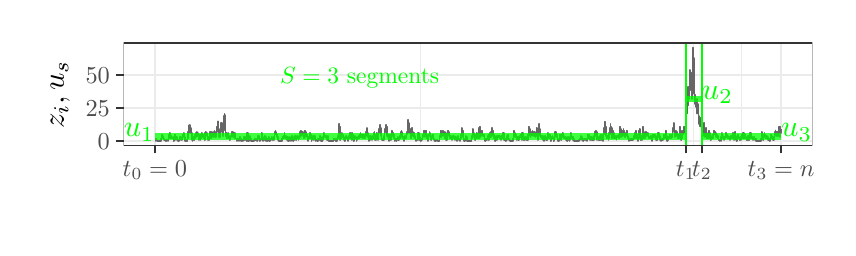
\begin{tikzpicture}[x=1pt,y=1pt]
\definecolor{fillColor}{RGB}{255,255,255}
\path[use as bounding box,fill=fillColor,fill opacity=0.00] (0,0) rectangle (289.08, 72.27);
\begin{scope}
\path[clip] (  0.00,  0.00) rectangle (289.08, 72.27);
\definecolor{drawColor}{RGB}{255,255,255}
\definecolor{fillColor}{RGB}{255,255,255}

\path[draw=drawColor,line width= 0.6pt,line join=round,line cap=round,fill=fillColor] (  0.00,  0.00) rectangle (289.08, 72.27);
\end{scope}
\begin{scope}
\path[clip] ( 34.65, 29.59) rectangle (283.58, 66.77);
\definecolor{fillColor}{RGB}{255,255,255}

\path[fill=fillColor] ( 34.65, 29.59) rectangle (283.58, 66.77);
\definecolor{drawColor}{gray}{0.92}

\path[draw=drawColor,line width= 0.3pt,line join=round] (141.89, 29.59) --
	(141.89, 66.77);

\path[draw=drawColor,line width= 0.3pt,line join=round] (240.71, 29.59) --
	(240.71, 66.77);

\path[draw=drawColor,line width= 0.3pt,line join=round] (257.94, 29.59) --
	(257.94, 66.77);

\path[draw=drawColor,line width= 0.6pt,line join=round] ( 34.65, 31.28) --
	(283.58, 31.28);

\path[draw=drawColor,line width= 0.6pt,line join=round] ( 34.65, 43.18) --
	(283.58, 43.18);

\path[draw=drawColor,line width= 0.6pt,line join=round] ( 34.65, 55.08) --
	(283.58, 55.08);

\path[draw=drawColor,line width= 0.6pt,line join=round] ( 45.97, 29.59) --
	( 45.97, 66.77);

\path[draw=drawColor,line width= 0.6pt,line join=round] (237.82, 29.59) --
	(237.82, 66.77);

\path[draw=drawColor,line width= 0.6pt,line join=round] (243.61, 29.59) --
	(243.61, 66.77);

\path[draw=drawColor,line width= 0.6pt,line join=round] (272.26, 29.59) --
	(272.26, 66.77);
\definecolor{drawColor}{gray}{0.40}

\path[draw=drawColor,line width= 0.6pt,line join=round] ( 45.97, 31.75) --
	( 46.15, 31.75) --
	( 46.15, 31.28) --
	( 46.17, 31.28) --
	( 46.17, 31.75) --
	( 46.18, 31.75) --
	( 46.18, 32.23) --
	( 46.60, 32.23) --
	( 46.60, 31.75) --
	( 46.63, 31.75) --
	( 46.63, 31.28) --
	( 48.22, 31.28) --
	( 48.22, 31.75) --
	( 48.26, 31.75) --
	( 48.26, 32.23) --
	( 48.49, 32.23) --
	( 48.49, 32.71) --
	( 48.56, 32.71) --
	( 48.56, 33.18) --
	( 48.63, 33.18) --
	( 48.63, 33.66) --
	( 48.67, 33.66) --
	( 48.67, 33.18) --
	( 48.71, 33.18) --
	( 48.71, 32.71) --
	( 48.83, 32.71) --
	( 48.83, 33.18) --
	( 48.94, 33.18) --
	( 48.94, 32.71) --
	( 49.00, 32.71) --
	( 49.00, 33.18) --
	( 49.01, 33.18) --
	( 49.01, 32.71) --
	( 49.08, 32.71) --
	( 49.08, 32.23) --
	( 49.29, 32.23) --
	( 49.29, 31.75) --
	( 49.31, 31.75) --
	( 49.31, 32.23) --
	( 49.45, 32.23) --
	( 49.45, 31.75) --
	( 49.76, 31.75) --
	( 49.76, 31.28) --
	( 50.20, 31.28) --
	( 50.20, 31.75) --
	( 50.65, 31.75) --
	( 50.65, 31.28) --
	( 50.68, 31.28) --
	( 50.68, 31.75) --
	( 50.86, 31.75) --
	( 50.86, 32.23) --
	( 50.96, 32.23) --
	( 50.96, 32.71) --
	( 51.04, 32.71) --
	( 51.04, 33.18) --
	( 51.06, 33.18) --
	( 51.06, 33.66) --
	( 51.14, 33.66) --
	( 51.14, 33.18) --
	( 51.20, 33.18) --
	( 51.20, 33.66) --
	( 51.30, 33.66) --
	( 51.30, 34.13) --
	( 51.31, 34.13) --
	( 51.31, 33.66) --
	( 51.32, 33.66) --
	( 51.32, 34.13) --
	( 51.41, 34.13) --
	( 51.41, 33.66) --
	( 51.47, 33.66) --
	( 51.47, 34.13) --
	( 51.50, 34.13) --
	( 51.50, 33.66) --
	( 51.51, 33.66) --
	( 51.51, 33.18) --
	( 51.53, 33.18) --
	( 51.53, 33.66) --
	( 51.65, 33.66) --
	( 51.65, 33.18) --
	( 51.75, 33.18) --
	( 51.75, 32.71) --
	( 51.77, 32.71) --
	( 51.77, 32.23) --
	( 51.80, 32.23) --
	( 51.80, 32.71) --
	( 51.82, 32.71) --
	( 51.82, 33.18) --
	( 51.93, 33.18) --
	( 51.93, 32.71) --
	( 51.97, 32.71) --
	( 51.97, 32.23) --
	( 52.26, 32.23) --
	( 52.26, 32.71) --
	( 52.27, 32.71) --
	( 52.27, 32.23) --
	( 52.70, 32.23) --
	( 52.70, 31.28) --
	( 52.81, 31.28) --
	( 52.81, 31.75) --
	( 52.83, 31.75) --
	( 52.83, 32.23) --
	( 52.88, 32.23) --
	( 52.88, 32.71) --
	( 53.02, 32.71) --
	( 53.02, 33.18) --
	( 53.10, 33.18) --
	( 53.10, 33.66) --
	( 53.26, 33.66) --
	( 53.26, 33.18) --
	( 53.29, 33.18) --
	( 53.29, 32.71) --
	( 53.34, 32.71) --
	( 53.34, 32.23) --
	( 53.34, 32.23) --
	( 53.34, 32.71) --
	( 53.47, 32.71) --
	( 53.47, 32.23) --
	( 53.55, 32.23) --
	( 53.55, 31.75) --
	( 53.60, 31.75) --
	( 53.60, 32.23) --
	( 53.69, 32.23) --
	( 53.69, 32.71) --
	( 53.79, 32.71) --
	( 53.79, 32.23) --
	( 53.98, 32.23) --
	( 53.98, 32.71) --
	( 54.05, 32.71) --
	( 54.05, 32.23) --
	( 54.14, 32.23) --
	( 54.14, 31.75) --
	( 54.43, 31.75) --
	( 54.43, 31.28) --
	( 54.79, 31.28) --
	( 54.79, 31.75) --
	( 55.03, 31.75) --
	( 55.03, 32.23) --
	( 55.09, 32.23) --
	( 55.09, 32.71) --
	( 55.25, 32.71) --
	( 55.25, 32.23) --
	( 55.35, 32.23) --
	( 55.35, 32.71) --
	( 55.48, 32.71) --
	( 55.48, 32.23) --
	( 55.54, 32.23) --
	( 55.54, 31.75) --
	( 55.78, 31.75) --
	( 55.78, 32.23) --
	( 55.80, 32.23) --
	( 55.80, 31.75) --
	( 55.81, 31.75) --
	( 55.81, 32.23) --
	( 55.98, 32.23) --
	( 55.98, 33.18) --
	( 56.17, 33.18) --
	( 56.17, 33.66) --
	( 56.23, 33.66) --
	( 56.23, 33.18) --
	( 56.27, 33.18) --
	( 56.27, 32.71) --
	( 56.41, 32.71) --
	( 56.41, 33.66) --
	( 56.43, 33.66) --
	( 56.43, 34.13) --
	( 56.44, 34.13) --
	( 56.44, 33.18) --
	( 56.62, 33.18) --
	( 56.62, 32.71) --
	( 56.87, 32.71) --
	( 56.87, 31.75) --
	( 56.87, 31.75) --
	( 56.87, 31.28) --
	( 57.13, 31.28) --
	( 57.13, 31.75) --
	( 57.59, 31.75) --
	( 57.59, 31.28) --
	( 57.72, 31.28) --
	( 57.72, 31.75) --
	( 57.77, 31.75) --
	( 57.77, 32.23) --
	( 57.82, 32.23) --
	( 57.82, 33.18) --
	( 57.91, 33.18) --
	( 57.91, 34.13) --
	( 58.05, 34.13) --
	( 58.05, 34.61) --
	( 58.10, 34.61) --
	( 58.10, 35.09) --
	( 58.17, 35.09) --
	( 58.17, 34.61) --
	( 58.20, 34.61) --
	( 58.20, 36.04) --
	( 58.22, 36.04) --
	( 58.22, 36.51) --
	( 58.22, 36.51) --
	( 58.22, 36.04) --
	( 58.27, 36.04) --
	( 58.27, 36.99) --
	( 58.27, 36.99) --
	( 58.27, 36.04) --
	( 58.34, 36.04) --
	( 58.34, 36.51) --
	( 58.37, 36.51) --
	( 58.37, 35.56) --
	( 58.43, 35.56) --
	( 58.43, 36.04) --
	( 58.51, 36.04) --
	( 58.51, 35.56) --
	( 58.56, 35.56) --
	( 58.56, 35.09) --
	( 58.59, 35.09) --
	( 58.59, 36.51) --
	( 58.64, 36.51) --
	( 58.64, 36.99) --
	( 58.65, 36.99) --
	( 58.65, 36.51) --
	( 58.65, 36.51) --
	( 58.65, 35.56) --
	( 58.67, 35.56) --
	( 58.67, 35.09) --
	( 58.73, 35.09) --
	( 58.73, 34.13) --
	( 58.81, 34.13) --
	( 58.81, 34.61) --
	( 58.84, 34.61) --
	( 58.84, 35.09) --
	( 58.84, 35.09) --
	( 58.84, 35.56) --
	( 58.89, 35.56) --
	( 58.89, 35.09) --
	( 58.99, 35.09) --
	( 58.99, 35.56) --
	( 59.02, 35.56) --
	( 59.02, 36.04) --
	( 59.04, 36.04) --
	( 59.04, 34.61) --
	( 59.05, 34.61) --
	( 59.05, 35.09) --
	( 59.09, 35.09) --
	( 59.09, 34.61) --
	( 59.25, 34.61) --
	( 59.25, 34.13) --
	( 59.27, 34.13) --
	( 59.27, 33.66) --
	( 59.29, 33.66) --
	( 59.29, 32.71) --
	( 59.45, 32.71) --
	( 59.45, 31.75) --
	( 59.51, 31.75) --
	( 59.51, 31.28) --
	( 59.56, 31.28) --
	( 59.56, 31.75) --
	( 59.65, 31.75) --
	( 59.65, 32.23) --
	( 59.87, 32.23) --
	( 59.87, 32.71) --
	( 60.00, 32.71) --
	( 60.00, 32.23) --
	( 60.10, 32.23) --
	( 60.10, 31.75) --
	( 60.22, 31.75) --
	( 60.22, 32.23) --
	( 60.32, 32.23) --
	( 60.32, 31.75) --
	( 60.33, 31.75) --
	( 60.33, 32.23) --
	( 60.37, 32.23) --
	( 60.37, 32.71) --
	( 60.39, 32.71) --
	( 60.39, 33.18) --
	( 60.56, 33.18) --
	( 60.56, 33.66) --
	( 60.67, 33.66) --
	( 60.67, 33.18) --
	( 60.69, 33.18) --
	( 60.69, 33.66) --
	( 60.78, 33.66) --
	( 60.78, 33.18) --
	( 60.82, 33.18) --
	( 60.82, 32.71) --
	( 60.83, 32.71) --
	( 60.83, 33.66) --
	( 60.85, 33.66) --
	( 60.85, 33.18) --
	( 60.92, 33.18) --
	( 60.92, 33.66) --
	( 60.94, 33.66) --
	( 60.94, 34.13) --
	( 61.09, 34.13) --
	( 61.09, 34.61) --
	( 61.14, 34.61) --
	( 61.14, 34.13) --
	( 61.23, 34.13) --
	( 61.23, 34.61) --
	( 61.28, 34.61) --
	( 61.28, 33.66) --
	( 61.37, 33.66) --
	( 61.37, 34.13) --
	( 61.38, 34.13) --
	( 61.38, 33.66) --
	( 61.39, 33.66) --
	( 61.39, 33.18) --
	( 61.42, 33.18) --
	( 61.42, 34.13) --
	( 61.46, 34.13) --
	( 61.46, 33.66) --
	( 61.54, 33.66) --
	( 61.54, 33.18) --
	( 61.68, 33.18) --
	( 61.68, 32.71) --
	( 61.79, 32.71) --
	( 61.79, 33.18) --
	( 61.82, 33.18) --
	( 61.82, 32.71) --
	( 61.88, 32.71) --
	( 61.88, 31.75) --
	( 61.89, 31.75) --
	( 61.89, 32.23) --
	( 61.91, 32.23) --
	( 61.91, 32.71) --
	( 61.96, 32.71) --
	( 61.96, 33.18) --
	( 62.22, 33.18) --
	( 62.22, 33.66) --
	( 62.23, 33.66) --
	( 62.23, 33.18) --
	( 62.34, 33.18) --
	( 62.34, 32.71) --
	( 62.36, 32.71) --
	( 62.36, 32.23) --
	( 62.42, 32.23) --
	( 62.42, 31.75) --
	( 62.50, 31.75) --
	( 62.50, 32.23) --
	( 62.61, 32.23) --
	( 62.61, 32.71) --
	( 62.63, 32.71) --
	( 62.63, 33.18) --
	( 62.64, 33.18) --
	( 62.64, 33.66) --
	( 62.66, 33.66) --
	( 62.66, 33.18) --
	( 62.68, 33.18) --
	( 62.68, 33.66) --
	( 62.75, 33.66) --
	( 62.75, 34.13) --
	( 62.95, 34.13) --
	( 62.95, 33.66) --
	( 63.03, 33.66) --
	( 63.03, 34.13) --
	( 63.09, 34.13) --
	( 63.09, 33.66) --
	( 63.09, 33.66) --
	( 63.09, 33.18) --
	( 63.10, 33.18) --
	( 63.10, 33.66) --
	( 63.14, 33.66) --
	( 63.14, 33.18) --
	( 63.20, 33.18) --
	( 63.20, 32.71) --
	( 63.42, 32.71) --
	( 63.42, 33.18) --
	( 63.45, 33.18) --
	( 63.45, 33.66) --
	( 63.48, 33.66) --
	( 63.48, 33.18) --
	( 63.51, 33.18) --
	( 63.51, 32.71) --
	( 63.55, 32.71) --
	( 63.55, 32.23) --
	( 63.86, 32.23) --
	( 63.86, 32.71) --
	( 63.87, 32.71) --
	( 63.87, 32.23) --
	( 63.91, 32.23) --
	( 63.91, 31.75) --
	( 63.96, 31.75) --
	( 63.96, 32.23) --
	( 63.97, 32.23) --
	( 63.97, 32.71) --
	( 64.06, 32.71) --
	( 64.06, 33.18) --
	( 64.14, 33.18) --
	( 64.14, 33.66) --
	( 64.17, 33.66) --
	( 64.17, 34.13) --
	( 64.25, 34.13) --
	( 64.25, 34.61) --
	( 64.31, 34.61) --
	( 64.31, 34.13) --
	( 64.39, 34.13) --
	( 64.39, 34.61) --
	( 64.41, 34.61) --
	( 64.41, 34.13) --
	( 64.42, 34.13) --
	( 64.42, 33.66) --
	( 64.48, 33.66) --
	( 64.48, 33.18) --
	( 64.52, 33.18) --
	( 64.52, 33.66) --
	( 64.58, 33.66) --
	( 64.58, 34.13) --
	( 64.59, 34.13) --
	( 64.59, 33.66) --
	( 64.60, 33.66) --
	( 64.60, 34.13) --
	( 64.62, 34.13) --
	( 64.62, 33.66) --
	( 64.65, 33.66) --
	( 64.65, 34.13) --
	( 64.71, 34.13) --
	( 64.71, 33.66) --
	( 64.76, 33.66) --
	( 64.76, 34.13) --
	( 64.85, 34.13) --
	( 64.85, 33.66) --
	( 64.97, 33.66) --
	( 64.97, 33.18) --
	( 65.04, 33.18) --
	( 65.04, 32.71) --
	( 65.05, 32.71) --
	( 65.05, 32.23) --
	( 65.10, 32.23) --
	( 65.10, 31.75) --
	( 65.13, 31.75) --
	( 65.13, 32.23) --
	( 65.15, 32.23) --
	( 65.15, 31.75) --
	( 65.28, 31.75) --
	( 65.28, 32.23) --
	( 65.53, 32.23) --
	( 65.53, 32.71) --
	( 65.58, 32.71) --
	( 65.58, 32.23) --
	( 65.73, 32.23) --
	( 65.73, 31.75) --
	( 65.76, 31.75) --
	( 65.76, 32.71) --
	( 65.78, 32.71) --
	( 65.78, 33.18) --
	( 65.80, 33.18) --
	( 65.80, 33.66) --
	( 65.82, 33.66) --
	( 65.82, 34.13) --
	( 65.86, 34.13) --
	( 65.86, 34.61) --
	( 65.98, 34.61) --
	( 65.98, 34.13) --
	( 66.05, 34.13) --
	( 66.05, 34.61) --
	( 66.21, 34.61) --
	( 66.21, 33.66) --
	( 66.24, 33.66) --
	( 66.24, 33.18) --
	( 66.24, 33.18) --
	( 66.24, 32.71) --
	( 66.31, 32.71) --
	( 66.31, 32.23) --
	( 66.39, 32.23) --
	( 66.39, 32.71) --
	( 66.41, 32.71) --
	( 66.41, 33.66) --
	( 66.53, 33.66) --
	( 66.53, 34.13) --
	( 66.58, 34.13) --
	( 66.58, 34.61) --
	( 66.72, 34.61) --
	( 66.72, 34.13) --
	( 66.84, 34.13) --
	( 66.84, 33.66) --
	( 66.86, 33.66) --
	( 66.86, 32.71) --
	( 66.89, 32.71) --
	( 66.89, 33.18) --
	( 66.96, 33.18) --
	( 66.96, 32.71) --
	( 66.98, 32.71) --
	( 66.98, 33.18) --
	( 66.99, 33.18) --
	( 66.99, 32.71) --
	( 67.02, 32.71) --
	( 67.02, 33.18) --
	( 67.03, 33.18) --
	( 67.03, 32.71) --
	( 67.09, 32.71) --
	( 67.09, 33.18) --
	( 67.16, 33.18) --
	( 67.16, 33.66) --
	( 67.19, 33.66) --
	( 67.19, 34.13) --
	( 67.27, 34.13) --
	( 67.27, 34.61) --
	( 67.34, 34.61) --
	( 67.34, 34.13) --
	( 67.34, 34.13) --
	( 67.34, 34.61) --
	( 67.43, 34.61) --
	( 67.43, 34.13) --
	( 67.46, 34.13) --
	( 67.46, 34.61) --
	( 67.47, 34.61) --
	( 67.47, 35.09) --
	( 67.48, 35.09) --
	( 67.48, 34.61) --
	( 67.54, 34.61) --
	( 67.54, 34.13) --
	( 67.62, 34.13) --
	( 67.62, 33.66) --
	( 67.64, 33.66) --
	( 67.64, 33.18) --
	( 67.72, 33.18) --
	( 67.72, 32.71) --
	( 67.73, 32.71) --
	( 67.73, 33.18) --
	( 67.76, 33.18) --
	( 67.76, 34.13) --
	( 67.80, 34.13) --
	( 67.80, 33.66) --
	( 67.91, 33.66) --
	( 67.91, 33.18) --
	( 67.92, 33.18) --
	( 67.92, 32.71) --
	( 67.94, 32.71) --
	( 67.94, 33.18) --
	( 67.99, 33.18) --
	( 67.99, 33.66) --
	( 68.06, 33.66) --
	( 68.06, 34.13) --
	( 68.16, 34.13) --
	( 68.16, 34.61) --
	( 68.18, 34.61) --
	( 68.18, 34.13) --
	( 68.20, 34.13) --
	( 68.20, 34.61) --
	( 68.20, 34.61) --
	( 68.20, 35.09) --
	( 68.21, 35.09) --
	( 68.21, 34.61) --
	( 68.21, 34.61) --
	( 68.21, 34.13) --
	( 68.24, 34.13) --
	( 68.24, 34.61) --
	( 68.39, 34.61) --
	( 68.39, 35.09) --
	( 68.39, 35.09) --
	( 68.39, 34.61) --
	( 68.44, 34.61) --
	( 68.44, 35.09) --
	( 68.44, 35.09) --
	( 68.44, 34.61) --
	( 68.46, 34.61) --
	( 68.46, 36.04) --
	( 68.47, 36.04) --
	( 68.47, 36.51) --
	( 68.49, 36.51) --
	( 68.49, 36.04) --
	( 68.51, 36.04) --
	( 68.51, 36.51) --
	( 68.56, 36.51) --
	( 68.56, 36.99) --
	( 68.60, 36.99) --
	( 68.60, 37.47) --
	( 68.61, 37.47) --
	( 68.61, 36.99) --
	( 68.65, 36.99) --
	( 68.65, 36.51) --
	( 68.66, 36.51) --
	( 68.66, 36.04) --
	( 68.66, 36.04) --
	( 68.66, 36.51) --
	( 68.69, 36.51) --
	( 68.69, 36.99) --
	( 68.69, 36.99) --
	( 68.69, 36.51) --
	( 68.70, 36.51) --
	( 68.70, 37.47) --
	( 68.77, 37.47) --
	( 68.77, 37.94) --
	( 68.83, 37.94) --
	( 68.83, 38.42) --
	( 68.83, 38.42) --
	( 68.83, 37.94) --
	( 68.89, 37.94) --
	( 68.89, 37.47) --
	( 68.92, 37.47) --
	( 68.92, 36.04) --
	( 68.92, 36.04) --
	( 68.92, 35.09) --
	( 68.93, 35.09) --
	( 68.93, 35.56) --
	( 68.99, 35.56) --
	( 68.99, 36.04) --
	( 69.01, 36.04) --
	( 69.01, 35.56) --
	( 69.05, 35.56) --
	( 69.05, 35.09) --
	( 69.06, 35.09) --
	( 69.06, 34.61) --
	( 69.14, 34.61) --
	( 69.14, 34.13) --
	( 69.16, 34.13) --
	( 69.16, 33.18) --
	( 69.20, 33.18) --
	( 69.20, 33.66) --
	( 69.21, 33.66) --
	( 69.21, 32.71) --
	( 69.30, 32.71) --
	( 69.30, 33.18) --
	( 69.38, 33.18) --
	( 69.38, 33.66) --
	( 69.39, 33.66) --
	( 69.39, 33.18) --
	( 69.44, 33.18) --
	( 69.44, 32.71) --
	( 69.51, 32.71) --
	( 69.51, 33.66) --
	( 69.55, 33.66) --
	( 69.55, 34.13) --
	( 69.59, 34.13) --
	( 69.59, 34.61) --
	( 69.59, 34.61) --
	( 69.59, 34.13) --
	( 69.66, 34.13) --
	( 69.66, 34.61) --
	( 69.68, 34.61) --
	( 69.68, 35.09) --
	( 69.75, 35.09) --
	( 69.75, 34.61) --
	( 69.78, 34.61) --
	( 69.78, 35.09) --
	( 69.79, 35.09) --
	( 69.79, 35.56) --
	( 69.82, 35.56) --
	( 69.82, 36.04) --
	( 69.85, 36.04) --
	( 69.85, 35.56) --
	( 69.87, 35.56) --
	( 69.87, 36.04) --
	( 69.90, 36.04) --
	( 69.90, 36.51) --
	( 69.92, 36.51) --
	( 69.92, 36.99) --
	( 69.92, 36.99) --
	( 69.92, 37.47) --
	( 69.97, 37.47) --
	( 69.97, 37.94) --
	( 70.00, 37.94) --
	( 70.00, 37.47) --
	( 70.02, 37.47) --
	( 70.02, 37.94) --
	( 70.04, 37.94) --
	( 70.04, 37.47) --
	( 70.05, 37.47) --
	( 70.05, 36.99) --
	( 70.08, 36.99) --
	( 70.08, 37.47) --
	( 70.09, 37.47) --
	( 70.09, 37.94) --
	( 70.11, 37.94) --
	( 70.11, 37.47) --
	( 70.19, 37.47) --
	( 70.19, 37.94) --
	( 70.24, 37.94) --
	( 70.24, 37.47) --
	( 70.27, 37.47) --
	( 70.27, 36.99) --
	( 70.28, 36.99) --
	( 70.28, 37.47) --
	( 70.29, 37.47) --
	( 70.29, 36.99) --
	( 70.32, 36.99) --
	( 70.32, 37.47) --
	( 70.35, 37.47) --
	( 70.35, 36.99) --
	( 70.37, 36.99) --
	( 70.37, 36.51) --
	( 70.38, 36.51) --
	( 70.38, 36.04) --
	( 70.41, 36.04) --
	( 70.41, 35.56) --
	( 70.43, 35.56) --
	( 70.43, 35.09) --
	( 70.47, 35.09) --
	( 70.47, 34.61) --
	( 70.52, 34.61) --
	( 70.52, 34.13) --
	( 70.53, 34.13) --
	( 70.53, 34.61) --
	( 70.54, 34.61) --
	( 70.54, 34.13) --
	( 70.54, 34.13) --
	( 70.54, 33.66) --
	( 70.59, 33.66) --
	( 70.59, 33.18) --
	( 70.60, 33.18) --
	( 70.60, 33.66) --
	( 70.63, 33.66) --
	( 70.63, 34.13) --
	( 70.64, 34.13) --
	( 70.64, 33.66) --
	( 70.72, 33.66) --
	( 70.72, 34.13) --
	( 70.73, 34.13) --
	( 70.73, 33.66) --
	( 70.77, 33.66) --
	( 70.77, 33.18) --
	( 70.79, 33.18) --
	( 70.79, 33.66) --
	( 70.79, 33.66) --
	( 70.79, 34.61) --
	( 70.80, 34.61) --
	( 70.80, 35.09) --
	( 70.86, 35.09) --
	( 70.86, 35.56) --
	( 70.89, 35.56) --
	( 70.89, 36.04) --
	( 70.91, 36.04) --
	( 70.91, 36.51) --
	( 70.91, 36.51) --
	( 70.91, 36.99) --
	( 70.95, 36.99) --
	( 70.95, 37.47) --
	( 70.97, 37.47) --
	( 70.97, 37.94) --
	( 70.98, 37.94) --
	( 70.98, 37.47) --
	( 70.98, 37.47) --
	( 70.98, 37.94) --
	( 71.00, 37.94) --
	( 71.00, 39.37) --
	( 71.02, 39.37) --
	( 71.02, 39.85) --
	( 71.04, 39.85) --
	( 71.04, 39.37) --
	( 71.05, 39.37) --
	( 71.05, 39.85) --
	( 71.06, 39.85) --
	( 71.06, 40.32) --
	( 71.07, 40.32) --
	( 71.07, 40.80) --
	( 71.08, 40.80) --
	( 71.08, 41.27) --
	( 71.09, 41.27) --
	( 71.09, 40.80) --
	( 71.14, 40.80) --
	( 71.14, 41.27) --
	( 71.17, 41.27) --
	( 71.17, 40.80) --
	( 71.24, 40.80) --
	( 71.24, 40.32) --
	( 71.25, 40.32) --
	( 71.25, 39.85) --
	( 71.26, 39.85) --
	( 71.26, 39.37) --
	( 71.31, 39.37) --
	( 71.31, 38.89) --
	( 71.35, 38.89) --
	( 71.35, 38.42) --
	( 71.36, 38.42) --
	( 71.36, 37.94) --
	( 71.36, 37.94) --
	( 71.36, 37.47) --
	( 71.40, 37.47) --
	( 71.40, 36.99) --
	( 71.42, 36.99) --
	( 71.42, 36.51) --
	( 71.44, 36.51) --
	( 71.44, 36.04) --
	( 71.45, 36.04) --
	( 71.45, 34.61) --
	( 71.46, 34.61) --
	( 71.46, 35.09) --
	( 71.47, 35.09) --
	( 71.47, 34.13) --
	( 71.50, 34.13) --
	( 71.50, 33.66) --
	( 71.51, 33.66) --
	( 71.51, 33.18) --
	( 71.52, 33.18) --
	( 71.52, 33.66) --
	( 71.53, 33.66) --
	( 71.53, 34.13) --
	( 71.54, 34.13) --
	( 71.54, 33.66) --
	( 71.59, 33.66) --
	( 71.59, 33.18) --
	( 71.71, 33.18) --
	( 71.71, 34.13) --
	( 71.91, 34.13) --
	( 71.91, 33.66) --
	( 71.97, 33.66) --
	( 71.97, 32.23) --
	( 72.14, 32.23) --
	( 72.14, 33.18) --
	( 72.16, 33.18) --
	( 72.16, 32.23) --
	( 72.25, 32.23) --
	( 72.25, 32.71) --
	( 72.38, 32.71) --
	( 72.38, 33.18) --
	( 72.52, 33.18) --
	( 72.52, 33.66) --
	( 72.53, 33.66) --
	( 72.53, 34.13) --
	( 72.59, 34.13) --
	( 72.59, 33.18) --
	( 72.69, 33.18) --
	( 72.69, 32.71) --
	( 72.83, 32.71) --
	( 72.83, 32.23) --
	( 72.84, 32.23) --
	( 72.84, 32.71) --
	( 72.97, 32.71) --
	( 72.97, 32.23) --
	( 72.98, 32.23) --
	( 72.98, 31.75) --
	( 73.00, 31.75) --
	( 73.00, 32.23) --
	( 73.01, 32.23) --
	( 73.01, 32.71) --
	( 73.28, 32.71) --
	( 73.28, 33.18) --
	( 73.29, 33.18) --
	( 73.29, 32.71) --
	( 73.43, 32.71) --
	( 73.43, 33.18) --
	( 73.46, 33.18) --
	( 73.46, 32.71) --
	( 73.53, 32.71) --
	( 73.53, 33.18) --
	( 73.66, 33.18) --
	( 73.66, 33.66) --
	( 73.73, 33.66) --
	( 73.73, 33.18) --
	( 73.77, 33.18) --
	( 73.77, 33.66) --
	( 73.83, 33.66) --
	( 73.83, 34.61) --
	( 73.88, 34.61) --
	( 73.88, 34.13) --
	( 73.91, 34.13) --
	( 73.91, 33.66) --
	( 73.98, 33.66) --
	( 73.98, 33.18) --
	( 74.03, 33.18) --
	( 74.03, 33.66) --
	( 74.05, 33.66) --
	( 74.05, 34.13) --
	( 74.11, 34.13) --
	( 74.11, 33.66) --
	( 74.16, 33.66) --
	( 74.16, 34.13) --
	( 74.20, 34.13) --
	( 74.20, 34.61) --
	( 74.21, 34.61) --
	( 74.21, 34.13) --
	( 74.21, 34.13) --
	( 74.21, 33.66) --
	( 74.24, 33.66) --
	( 74.24, 33.18) --
	( 74.28, 33.18) --
	( 74.28, 32.71) --
	( 74.36, 32.71) --
	( 74.36, 33.18) --
	( 74.38, 33.18) --
	( 74.38, 33.66) --
	( 74.41, 33.66) --
	( 74.41, 33.18) --
	( 74.50, 33.18) --
	( 74.50, 32.71) --
	( 74.52, 32.71) --
	( 74.52, 33.18) --
	( 74.52, 33.18) --
	( 74.52, 33.66) --
	( 74.62, 33.66) --
	( 74.62, 34.13) --
	( 74.65, 34.13) --
	( 74.65, 33.66) --
	( 74.65, 33.66) --
	( 74.65, 34.13) --
	( 74.81, 34.13) --
	( 74.81, 33.66) --
	( 74.83, 33.66) --
	( 74.83, 33.18) --
	( 74.97, 33.18) --
	( 74.97, 32.23) --
	( 75.05, 32.23) --
	( 75.05, 32.71) --
	( 75.07, 32.71) --
	( 75.07, 32.23) --
	( 75.08, 32.23) --
	( 75.08, 32.71) --
	( 75.10, 32.71) --
	( 75.10, 32.23) --
	( 75.50, 32.23) --
	( 75.50, 31.75) --
	( 75.53, 31.75) --
	( 75.53, 31.28) --
	( 75.72, 31.28) --
	( 75.72, 31.75) --
	( 75.83, 31.75) --
	( 75.83, 32.23) --
	( 76.12, 32.23) --
	( 76.12, 31.75) --
	( 76.28, 31.75) --
	( 76.28, 31.28) --
	( 76.47, 31.28) --
	( 76.47, 31.75) --
	( 76.53, 31.75) --
	( 76.53, 32.23) --
	( 76.54, 32.23) --
	( 76.54, 32.71) --
	( 76.92, 32.71) --
	( 76.92, 32.23) --
	( 76.98, 32.23) --
	( 76.98, 31.75) --
	( 76.99, 31.75) --
	( 76.99, 31.28) --
	( 77.22, 31.28) --
	( 77.22, 31.75) --
	( 77.68, 31.75) --
	( 77.68, 31.28) --
	( 77.89, 31.28) --
	( 77.89, 31.75) --
	( 78.03, 31.75) --
	( 78.03, 32.23) --
	( 78.20, 32.23) --
	( 78.20, 32.71) --
	( 78.24, 32.71) --
	( 78.24, 32.23) --
	( 78.35, 32.23) --
	( 78.35, 31.75) --
	( 78.51, 31.75) --
	( 78.51, 32.23) --
	( 78.57, 32.23) --
	( 78.57, 32.71) --
	( 78.65, 32.71) --
	( 78.65, 32.23) --
	( 78.96, 32.23) --
	( 78.96, 31.75) --
	( 79.02, 31.75) --
	( 79.02, 31.28) --
	( 79.20, 31.28) --
	( 79.20, 32.71) --
	( 79.23, 32.71) --
	( 79.23, 34.13) --
	( 79.65, 34.13) --
	( 79.65, 32.71) --
	( 79.68, 32.71) --
	( 79.68, 32.23) --
	( 79.68, 32.23) --
	( 79.68, 31.28) --
	( 79.93, 31.28) --
	( 79.93, 31.75) --
	( 79.96, 31.75) --
	( 79.96, 32.23) --
	( 80.14, 32.23) --
	( 80.14, 32.71) --
	( 80.29, 32.71) --
	( 80.29, 33.18) --
	( 80.35, 33.18) --
	( 80.35, 32.71) --
	( 80.41, 32.71) --
	( 80.41, 32.23) --
	( 80.59, 32.23) --
	( 80.59, 31.75) --
	( 80.74, 31.75) --
	( 80.74, 31.28) --
	( 81.79, 31.28) --
	( 81.79, 31.75) --
	( 82.03, 31.75) --
	( 82.03, 32.23) --
	( 82.24, 32.23) --
	( 82.24, 31.75) --
	( 82.27, 31.75) --
	( 82.27, 32.23) --
	( 82.48, 32.23) --
	( 82.48, 31.75) --
	( 82.53, 31.75) --
	( 82.53, 32.23) --
	( 82.72, 32.23) --
	( 82.72, 31.75) --
	( 82.98, 31.75) --
	( 82.98, 31.28) --
	( 83.02, 31.28) --
	( 83.02, 31.75) --
	( 83.25, 31.75) --
	( 83.25, 32.23) --
	( 83.28, 32.23) --
	( 83.28, 32.71) --
	( 83.29, 32.71) --
	( 83.29, 33.18) --
	( 83.47, 33.18) --
	( 83.47, 32.71) --
	( 83.71, 32.71) --
	( 83.71, 32.23) --
	( 83.73, 32.23) --
	( 83.73, 31.75) --
	( 83.74, 31.75) --
	( 83.74, 31.28) --
	( 83.85, 31.28) --
	( 83.85, 31.75) --
	( 84.23, 31.75) --
	( 84.23, 32.23) --
	( 84.30, 32.23) --
	( 84.30, 31.75) --
	( 84.38, 31.75) --
	( 84.38, 32.23) --
	( 84.46, 32.23) --
	( 84.46, 32.71) --
	( 84.49, 32.71) --
	( 84.49, 33.66) --
	( 84.51, 33.66) --
	( 84.51, 34.13) --
	( 84.68, 34.13) --
	( 84.68, 33.66) --
	( 84.83, 33.66) --
	( 84.83, 33.18) --
	( 84.91, 33.18) --
	( 84.91, 32.71) --
	( 84.95, 32.71) --
	( 84.95, 31.75) --
	( 84.96, 31.75) --
	( 84.96, 31.28) --
	( 84.99, 31.28) --
	( 84.99, 31.75) --
	( 85.22, 31.75) --
	( 85.22, 32.23) --
	( 85.44, 32.23) --
	( 85.44, 31.75) --
	( 85.57, 31.75) --
	( 85.57, 32.23) --
	( 85.63, 32.23) --
	( 85.63, 33.18) --
	( 85.67, 33.18) --
	( 85.67, 32.71) --
	( 86.02, 32.71) --
	( 86.02, 32.23) --
	( 86.08, 32.23) --
	( 86.08, 31.28) --
	( 86.14, 31.28) --
	( 86.14, 31.75) --
	( 86.38, 31.75) --
	( 86.38, 32.23) --
	( 86.59, 32.23) --
	( 86.59, 31.28) --
	( 86.66, 31.28) --
	( 86.66, 31.75) --
	( 86.80, 31.75) --
	( 86.80, 32.23) --
	( 87.05, 32.23) --
	( 87.05, 32.71) --
	( 87.09, 32.71) --
	( 87.09, 32.23) --
	( 87.24, 32.23) --
	( 87.24, 31.28) --
	( 87.50, 31.28) --
	( 87.50, 31.75) --
	( 87.93, 31.75) --
	( 87.93, 32.23) --
	( 87.95, 32.23) --
	( 87.95, 31.75) --
	( 88.03, 31.75) --
	( 88.03, 32.23) --
	( 88.20, 32.23) --
	( 88.20, 32.71) --
	( 88.38, 32.71) --
	( 88.38, 32.23) --
	( 88.49, 32.23) --
	( 88.49, 31.75) --
	( 88.50, 31.75) --
	( 88.50, 32.23) --
	( 88.63, 32.23) --
	( 88.63, 31.75) --
	( 88.76, 31.75) --
	( 88.76, 32.23) --
	( 88.95, 32.23) --
	( 88.95, 31.75) --
	( 89.11, 31.75) --
	( 89.11, 32.23) --
	( 89.12, 32.23) --
	( 89.12, 32.71) --
	( 89.17, 32.71) --
	( 89.17, 33.66) --
	( 89.21, 33.66) --
	( 89.21, 33.18) --
	( 89.25, 33.18) --
	( 89.25, 33.66) --
	( 89.28, 33.66) --
	( 89.28, 34.13) --
	( 89.39, 34.13) --
	( 89.39, 34.61) --
	( 89.50, 34.61) --
	( 89.50, 35.09) --
	( 89.56, 35.09) --
	( 89.56, 34.61) --
	( 89.57, 34.61) --
	( 89.57, 35.09) --
	( 89.58, 35.09) --
	( 89.58, 34.61) --
	( 89.63, 34.61) --
	( 89.63, 33.66) --
	( 89.69, 33.66) --
	( 89.69, 34.13) --
	( 89.70, 34.13) --
	( 89.70, 33.66) --
	( 89.71, 33.66) --
	( 89.71, 34.13) --
	( 89.73, 34.13) --
	( 89.73, 33.66) --
	( 89.81, 33.66) --
	( 89.81, 34.13) --
	( 89.84, 34.13) --
	( 89.84, 33.66) --
	( 89.95, 33.66) --
	( 89.95, 33.18) --
	( 89.99, 33.18) --
	( 89.99, 33.66) --
	( 90.02, 33.66) --
	( 90.02, 33.18) --
	( 90.08, 33.18) --
	( 90.08, 33.66) --
	( 90.15, 33.66) --
	( 90.15, 33.18) --
	( 90.15, 33.18) --
	( 90.15, 32.71) --
	( 90.22, 32.71) --
	( 90.22, 33.18) --
	( 90.26, 33.18) --
	( 90.26, 32.71) --
	( 90.44, 32.71) --
	( 90.44, 32.23) --
	( 90.54, 32.23) --
	( 90.54, 31.75) --
	( 90.68, 31.75) --
	( 90.68, 31.28) --
	( 91.91, 31.28) --
	( 91.91, 31.75) --
	( 91.93, 31.75) --
	( 91.93, 32.23) --
	( 92.07, 32.23) --
	( 92.07, 32.71) --
	( 92.35, 32.71) --
	( 92.35, 32.23) --
	( 92.36, 32.23) --
	( 92.36, 32.71) --
	( 92.38, 32.71) --
	( 92.38, 33.18) --
	( 92.39, 33.18) --
	( 92.39, 32.71) --
	( 92.53, 32.71) --
	( 92.53, 32.23) --
	( 92.61, 32.23) --
	( 92.61, 32.71) --
	( 92.69, 32.71) --
	( 92.69, 33.18) --
	( 92.79, 33.18) --
	( 92.79, 34.13) --
	( 92.81, 34.13) --
	( 92.81, 33.66) --
	( 92.83, 33.66) --
	( 92.83, 33.18) --
	( 93.07, 33.18) --
	( 93.07, 32.71) --
	( 93.11, 32.71) --
	( 93.11, 33.18) --
	( 93.14, 33.18) --
	( 93.14, 32.71) --
	( 93.16, 32.71) --
	( 93.16, 33.18) --
	( 93.24, 33.18) --
	( 93.24, 32.23) --
	( 93.52, 32.23) --
	( 93.52, 32.71) --
	( 93.56, 32.71) --
	( 93.56, 32.23) --
	( 93.61, 32.23) --
	( 93.61, 31.75) --
	( 93.64, 31.75) --
	( 93.64, 32.23) --
	( 93.72, 32.23) --
	( 93.72, 32.71) --
	( 93.97, 32.71) --
	( 93.97, 32.23) --
	( 94.09, 32.23) --
	( 94.09, 31.75) --
	( 94.17, 31.75) --
	( 94.17, 31.28) --
	( 94.42, 31.28) --
	( 94.42, 31.75) --
	( 94.42, 31.75) --
	( 94.42, 32.23) --
	( 94.75, 32.23) --
	( 94.75, 32.71) --
	( 94.87, 32.71) --
	( 94.87, 31.75) --
	( 95.20, 31.75) --
	( 95.20, 31.28) --
	( 95.22, 31.28) --
	( 95.22, 31.75) --
	( 95.39, 31.75) --
	( 95.39, 32.23) --
	( 95.47, 32.23) --
	( 95.47, 32.71) --
	( 95.50, 32.71) --
	( 95.50, 33.18) --
	( 95.67, 33.18) --
	( 95.67, 32.71) --
	( 95.84, 32.71) --
	( 95.84, 32.23) --
	( 95.92, 32.23) --
	( 95.92, 31.75) --
	( 95.95, 31.75) --
	( 95.95, 31.28) --
	( 96.00, 31.28) --
	( 96.00, 31.75) --
	( 96.37, 31.75) --
	( 96.37, 32.23) --
	( 96.44, 32.23) --
	( 96.44, 32.71) --
	( 96.45, 32.71) --
	( 96.45, 32.23) --
	( 96.46, 32.23) --
	( 96.46, 32.71) --
	( 96.56, 32.71) --
	( 96.56, 33.18) --
	( 96.82, 33.18) --
	( 96.82, 32.71) --
	( 96.84, 32.71) --
	( 96.84, 33.18) --
	( 96.89, 33.18) --
	( 96.89, 32.71) --
	( 96.90, 32.71) --
	( 96.90, 32.23) --
	( 97.01, 32.23) --
	( 97.01, 31.75) --
	( 97.14, 31.75) --
	( 97.14, 32.23) --
	( 97.22, 32.23) --
	( 97.22, 32.71) --
	( 97.30, 32.71) --
	( 97.30, 32.23) --
	( 97.36, 32.23) --
	( 97.36, 32.71) --
	( 97.44, 32.71) --
	( 97.44, 33.18) --
	( 97.58, 33.18) --
	( 97.58, 32.71) --
	( 97.60, 32.71) --
	( 97.60, 33.18) --
	( 97.67, 33.18) --
	( 97.67, 32.71) --
	( 97.81, 32.71) --
	( 97.81, 32.23) --
	( 97.89, 32.23) --
	( 97.89, 31.75) --
	( 97.92, 31.75) --
	( 97.92, 32.23) --
	( 97.95, 32.23) --
	( 97.95, 32.71) --
	( 98.06, 32.71) --
	( 98.06, 32.23) --
	( 98.11, 32.23) --
	( 98.11, 32.71) --
	( 98.19, 32.71) --
	( 98.19, 32.23) --
	( 98.21, 32.23) --
	( 98.21, 32.71) --
	( 98.32, 32.71) --
	( 98.32, 33.18) --
	( 98.36, 33.18) --
	( 98.36, 33.66) --
	( 98.42, 33.66) --
	( 98.42, 34.13) --
	( 98.51, 34.13) --
	( 98.51, 34.61) --
	( 98.56, 34.61) --
	( 98.56, 34.13) --
	( 98.65, 34.13) --
	( 98.65, 33.66) --
	( 98.70, 33.66) --
	( 98.70, 34.13) --
	( 98.70, 34.13) --
	( 98.70, 34.61) --
	( 98.76, 34.61) --
	( 98.76, 35.09) --
	( 98.77, 35.09) --
	( 98.77, 34.61) --
	( 98.81, 34.61) --
	( 98.81, 34.13) --
	( 98.84, 34.13) --
	( 98.84, 34.61) --
	( 98.85, 34.61) --
	( 98.85, 33.66) --
	( 98.96, 33.66) --
	( 98.96, 33.18) --
	( 98.96, 33.18) --
	( 98.96, 33.66) --
	( 99.12, 33.66) --
	( 99.12, 34.13) --
	( 99.15, 34.13) --
	( 99.15, 33.66) --
	( 99.16, 33.66) --
	( 99.16, 33.18) --
	( 99.16, 33.18) --
	( 99.16, 33.66) --
	( 99.19, 33.66) --
	( 99.19, 34.13) --
	( 99.21, 34.13) --
	( 99.21, 34.61) --
	( 99.22, 34.61) --
	( 99.22, 34.13) --
	( 99.25, 34.13) --
	( 99.25, 34.61) --
	( 99.29, 34.61) --
	( 99.29, 34.13) --
	( 99.39, 34.13) --
	( 99.39, 34.61) --
	( 99.41, 34.61) --
	( 99.41, 34.13) --
	( 99.50, 34.13) --
	( 99.50, 34.61) --
	( 99.57, 34.61) --
	( 99.57, 34.13) --
	( 99.61, 34.13) --
	( 99.61, 33.66) --
	( 99.64, 33.66) --
	( 99.64, 33.18) --
	( 99.65, 33.18) --
	( 99.65, 33.66) --
	( 99.70, 33.66) --
	( 99.70, 33.18) --
	( 99.84, 33.18) --
	( 99.84, 32.71) --
	( 99.86, 32.71) --
	( 99.86, 32.23) --
	( 99.89, 32.23) --
	( 99.89, 32.71) --
	( 99.89, 32.71) --
	( 99.89, 33.18) --
	(100.10, 33.18) --
	(100.10, 32.71) --
	(100.18, 32.71) --
	(100.18, 33.18) --
	(100.24, 33.18) --
	(100.24, 33.66) --
	(100.26, 33.66) --
	(100.26, 34.13) --
	(100.32, 34.13) --
	(100.32, 35.09) --
	(100.34, 35.09) --
	(100.34, 34.61) --
	(100.34, 34.61) --
	(100.34, 34.13) --
	(100.38, 34.13) --
	(100.38, 34.61) --
	(100.40, 34.61) --
	(100.40, 34.13) --
	(100.49, 34.13) --
	(100.49, 34.61) --
	(100.63, 34.61) --
	(100.63, 34.13) --
	(100.68, 34.13) --
	(100.68, 33.66) --
	(100.71, 33.66) --
	(100.71, 33.18) --
	(100.74, 33.18) --
	(100.74, 34.13) --
	(100.77, 34.13) --
	(100.77, 33.66) --
	(100.77, 33.66) --
	(100.77, 33.18) --
	(100.78, 33.18) --
	(100.78, 33.66) --
	(100.83, 33.66) --
	(100.83, 33.18) --
	(100.94, 33.18) --
	(100.94, 32.71) --
	(101.19, 32.71) --
	(101.19, 31.75) --
	(101.23, 31.75) --
	(101.23, 31.28) --
	(101.29, 31.28) --
	(101.29, 31.75) --
	(101.52, 31.75) --
	(101.52, 32.23) --
	(101.68, 32.23) --
	(101.68, 32.71) --
	(101.75, 32.71) --
	(101.75, 32.23) --
	(101.93, 32.23) --
	(101.93, 33.18) --
	(101.97, 33.18) --
	(101.97, 32.71) --
	(101.98, 32.71) --
	(101.98, 33.66) --
	(102.05, 33.66) --
	(102.05, 34.13) --
	(102.14, 34.13) --
	(102.14, 33.66) --
	(102.16, 33.66) --
	(102.16, 33.18) --
	(102.19, 33.18) --
	(102.19, 33.66) --
	(102.38, 33.66) --
	(102.38, 33.18) --
	(102.43, 33.18) --
	(102.43, 32.71) --
	(102.43, 32.71) --
	(102.43, 32.23) --
	(102.51, 32.23) --
	(102.51, 31.28) --
	(102.51, 31.28) --
	(102.51, 31.75) --
	(102.68, 31.75) --
	(102.68, 32.23) --
	(102.81, 32.23) --
	(102.81, 32.71) --
	(102.85, 32.71) --
	(102.85, 33.18) --
	(102.96, 33.18) --
	(102.96, 32.71) --
	(103.14, 32.71) --
	(103.14, 32.23) --
	(103.26, 32.23) --
	(103.26, 31.75) --
	(103.29, 31.75) --
	(103.29, 32.23) --
	(103.33, 32.23) --
	(103.33, 32.71) --
	(103.55, 32.71) --
	(103.55, 33.18) --
	(103.75, 33.18) --
	(103.75, 32.71) --
	(103.76, 32.71) --
	(103.76, 32.23) --
	(103.78, 32.23) --
	(103.78, 31.75) --
	(104.00, 31.75) --
	(104.00, 31.28) --
	(104.01, 31.28) --
	(104.01, 31.75) --
	(104.47, 31.75) --
	(104.47, 31.28) --
	(104.81, 31.28) --
	(104.81, 31.75) --
	(105.00, 31.75) --
	(105.00, 32.23) --
	(105.13, 32.23) --
	(105.13, 31.75) --
	(105.41, 31.75) --
	(105.41, 32.23) --
	(105.45, 32.23) --
	(105.45, 31.75) --
	(105.46, 31.75) --
	(105.46, 32.23) --
	(105.49, 32.23) --
	(105.49, 32.71) --
	(105.63, 32.71) --
	(105.63, 33.18) --
	(105.86, 33.18) --
	(105.86, 32.71) --
	(105.91, 32.71) --
	(105.91, 32.23) --
	(105.95, 32.23) --
	(105.95, 31.75) --
	(106.08, 31.75) --
	(106.08, 31.28) --
	(106.54, 31.28) --
	(106.54, 31.75) --
	(106.70, 31.75) --
	(106.70, 32.23) --
	(106.79, 32.23) --
	(106.79, 32.71) --
	(106.85, 32.71) --
	(106.85, 33.18) --
	(106.91, 33.18) --
	(106.91, 33.66) --
	(106.99, 33.66) --
	(106.99, 33.18) --
	(107.11, 33.18) --
	(107.11, 33.66) --
	(107.14, 33.66) --
	(107.14, 34.13) --
	(107.15, 34.13) --
	(107.15, 33.66) --
	(107.24, 33.66) --
	(107.24, 33.18) --
	(107.30, 33.18) --
	(107.30, 32.71) --
	(107.35, 32.71) --
	(107.35, 33.18) --
	(107.36, 33.18) --
	(107.36, 32.71) --
	(107.48, 32.71) --
	(107.48, 33.18) --
	(107.56, 33.18) --
	(107.56, 32.71) --
	(107.71, 32.71) --
	(107.71, 33.18) --
	(107.80, 33.18) --
	(107.80, 32.71) --
	(107.80, 32.71) --
	(107.80, 33.18) --
	(107.93, 33.18) --
	(107.93, 32.71) --
	(108.03, 32.71) --
	(108.03, 32.23) --
	(108.04, 32.23) --
	(108.04, 32.71) --
	(108.15, 32.71) --
	(108.15, 32.23) --
	(108.25, 32.23) --
	(108.25, 31.75) --
	(108.28, 31.75) --
	(108.28, 32.23) --
	(108.46, 32.23) --
	(108.46, 32.71) --
	(108.47, 32.71) --
	(108.47, 33.18) --
	(108.49, 33.18) --
	(108.49, 32.71) --
	(108.57, 32.71) --
	(108.57, 32.23) --
	(108.64, 32.23) --
	(108.64, 31.75) --
	(108.75, 31.75) --
	(108.75, 31.28) --
	(110.49, 31.28) --
	(110.49, 31.75) --
	(110.76, 31.75) --
	(110.76, 32.23) --
	(110.94, 32.23) --
	(110.94, 31.75) --
	(111.20, 31.75) --
	(111.20, 31.28) --
	(111.82, 31.28) --
	(111.82, 31.75) --
	(111.87, 31.75) --
	(111.87, 32.23) --
	(112.22, 32.23) --
	(112.22, 32.71) --
	(112.25, 32.71) --
	(112.25, 33.18) --
	(112.27, 33.18) --
	(112.27, 32.71) --
	(112.31, 32.71) --
	(112.31, 34.13) --
	(112.32, 34.13) --
	(112.32, 33.66) --
	(112.34, 33.66) --
	(112.34, 35.09) --
	(112.36, 35.09) --
	(112.36, 35.56) --
	(112.40, 35.56) --
	(112.40, 36.04) --
	(112.41, 36.04) --
	(112.41, 36.51) --
	(112.48, 36.51) --
	(112.48, 36.99) --
	(112.50, 36.99) --
	(112.50, 37.47) --
	(112.67, 37.47) --
	(112.67, 36.99) --
	(112.70, 36.99) --
	(112.70, 36.51) --
	(112.76, 36.51) --
	(112.76, 36.04) --
	(112.77, 36.04) --
	(112.77, 35.09) --
	(112.79, 35.09) --
	(112.79, 33.66) --
	(112.81, 33.66) --
	(112.81, 34.13) --
	(112.82, 34.13) --
	(112.82, 33.66) --
	(112.86, 33.66) --
	(112.86, 33.18) --
	(112.87, 33.18) --
	(112.87, 32.71) --
	(112.93, 32.71) --
	(112.93, 32.23) --
	(112.96, 32.23) --
	(112.96, 31.75) --
	(113.05, 31.75) --
	(113.05, 32.23) --
	(113.20, 32.23) --
	(113.20, 32.71) --
	(113.21, 32.71) --
	(113.21, 33.18) --
	(113.26, 33.18) --
	(113.26, 32.71) --
	(113.26, 32.71) --
	(113.26, 32.23) --
	(113.34, 32.23) --
	(113.34, 32.71) --
	(113.49, 32.71) --
	(113.49, 33.18) --
	(113.55, 33.18) --
	(113.55, 33.66) --
	(113.58, 33.66) --
	(113.58, 34.13) --
	(113.64, 34.13) --
	(113.64, 33.66) --
	(113.65, 33.66) --
	(113.65, 32.71) --
	(113.66, 32.71) --
	(113.66, 33.18) --
	(113.75, 33.18) --
	(113.75, 33.66) --
	(113.79, 33.66) --
	(113.79, 33.18) --
	(113.84, 33.18) --
	(113.84, 33.66) --
	(114.01, 33.66) --
	(114.01, 33.18) --
	(114.03, 33.18) --
	(114.03, 32.71) --
	(114.06, 32.71) --
	(114.06, 33.18) --
	(114.12, 33.18) --
	(114.12, 32.71) --
	(114.21, 32.71) --
	(114.21, 32.23) --
	(114.28, 32.23) --
	(114.28, 31.75) --
	(114.50, 31.75) --
	(114.50, 31.28) --
	(114.70, 31.28) --
	(114.70, 31.75) --
	(114.75, 31.75) --
	(114.75, 32.23) --
	(114.95, 32.23) --
	(114.95, 32.71) --
	(115.13, 32.71) --
	(115.13, 33.18) --
	(115.16, 33.18) --
	(115.16, 32.71) --
	(115.21, 32.71) --
	(115.21, 32.23) --
	(115.31, 32.23) --
	(115.31, 32.71) --
	(115.40, 32.71) --
	(115.40, 32.23) --
	(115.59, 32.23) --
	(115.59, 31.75) --
	(115.76, 31.75) --
	(115.76, 31.28) --
	(115.85, 31.28) --
	(115.85, 31.75) --
	(115.89, 31.75) --
	(115.89, 32.23) --
	(115.99, 32.23) --
	(115.99, 32.71) --
	(116.02, 32.71) --
	(116.02, 33.18) --
	(116.26, 33.18) --
	(116.26, 33.66) --
	(116.31, 33.66) --
	(116.31, 33.18) --
	(116.34, 33.18) --
	(116.34, 32.71) --
	(116.42, 32.71) --
	(116.42, 33.18) --
	(116.44, 33.18) --
	(116.44, 32.71) --
	(116.47, 32.71) --
	(116.47, 32.23) --
	(116.50, 32.23) --
	(116.50, 32.71) --
	(116.53, 32.71) --
	(116.53, 33.18) --
	(116.53, 33.18) --
	(116.53, 33.66) --
	(116.55, 33.66) --
	(116.55, 34.13) --
	(116.71, 34.13) --
	(116.71, 33.66) --
	(116.77, 33.66) --
	(116.77, 33.18) --
	(116.92, 33.18) --
	(116.92, 33.66) --
	(116.96, 33.66) --
	(116.96, 33.18) --
	(116.98, 33.18) --
	(116.98, 32.71) --
	(116.98, 32.71) --
	(116.98, 32.23) --
	(117.01, 32.23) --
	(117.01, 31.75) --
	(117.04, 31.75) --
	(117.04, 32.23) --
	(117.05, 32.23) --
	(117.05, 32.71) --
	(117.10, 32.71) --
	(117.10, 33.18) --
	(117.15, 33.18) --
	(117.15, 33.66) --
	(117.26, 33.66) --
	(117.26, 34.13) --
	(117.37, 34.13) --
	(117.37, 33.66) --
	(117.45, 33.66) --
	(117.45, 33.18) --
	(117.49, 33.18) --
	(117.49, 32.71) --
	(117.55, 32.71) --
	(117.55, 32.23) --
	(117.60, 32.23) --
	(117.60, 31.75) --
	(117.71, 31.75) --
	(117.71, 31.28) --
	(117.94, 31.28) --
	(117.94, 31.75) --
	(118.14, 31.75) --
	(118.14, 32.23) --
	(118.35, 32.23) --
	(118.35, 32.71) --
	(118.35, 32.71) --
	(118.35, 33.18) --
	(118.39, 33.18) --
	(118.39, 32.71) --
	(118.59, 32.71) --
	(118.59, 32.23) --
	(118.79, 32.23) --
	(118.79, 31.75) --
	(118.80, 31.75) --
	(118.80, 31.28) --
	(118.84, 31.28) --
	(118.84, 31.75) --
	(119.05, 31.75) --
	(119.05, 32.23) --
	(119.27, 32.23) --
	(119.27, 32.71) --
	(119.29, 32.71) --
	(119.29, 32.23) --
	(119.44, 32.23) --
	(119.44, 32.71) --
	(119.51, 32.71) --
	(119.51, 32.23) --
	(119.55, 32.23) --
	(119.55, 32.71) --
	(119.72, 32.71) --
	(119.72, 32.23) --
	(119.82, 32.23) --
	(119.82, 32.71) --
	(119.84, 32.71) --
	(119.84, 33.18) --
	(119.85, 33.18) --
	(119.85, 33.66) --
	(119.89, 33.66) --
	(119.89, 33.18) --
	(120.00, 33.18) --
	(120.00, 32.71) --
	(120.23, 32.71) --
	(120.23, 33.18) --
	(120.25, 33.18) --
	(120.25, 34.13) --
	(120.27, 34.13) --
	(120.27, 33.66) --
	(120.29, 33.66) --
	(120.29, 33.18) --
	(120.31, 33.18) --
	(120.31, 32.71) --
	(120.47, 32.71) --
	(120.47, 33.18) --
	(120.48, 33.18) --
	(120.48, 32.71) --
	(120.53, 32.71) --
	(120.53, 33.18) --
	(120.66, 33.18) --
	(120.66, 33.66) --
	(120.70, 33.66) --
	(120.70, 32.71) --
	(120.87, 32.71) --
	(120.87, 33.18) --
	(120.91, 33.18) --
	(120.91, 32.71) --
	(120.95, 32.71) --
	(120.95, 33.18) --
	(120.98, 33.18) --
	(120.98, 32.71) --
	(121.11, 32.71) --
	(121.11, 32.23) --
	(121.12, 32.23) --
	(121.12, 32.71) --
	(121.20, 32.71) --
	(121.20, 33.18) --
	(121.26, 33.18) --
	(121.26, 33.66) --
	(121.32, 33.66) --
	(121.32, 33.18) --
	(121.34, 33.18) --
	(121.34, 33.66) --
	(121.41, 33.66) --
	(121.41, 33.18) --
	(121.47, 33.18) --
	(121.47, 33.66) --
	(121.56, 33.66) --
	(121.56, 33.18) --
	(121.65, 33.18) --
	(121.65, 32.71) --
	(121.67, 32.71) --
	(121.67, 33.18) --
	(121.70, 33.18) --
	(121.70, 33.66) --
	(121.71, 33.66) --
	(121.71, 33.18) --
	(121.80, 33.18) --
	(121.80, 32.71) --
	(121.91, 32.71) --
	(121.91, 32.23) --
	(122.03, 32.23) --
	(122.03, 32.71) --
	(122.10, 32.71) --
	(122.10, 33.18) --
	(122.12, 33.18) --
	(122.12, 32.71) --
	(122.13, 32.71) --
	(122.13, 33.18) --
	(122.15, 33.18) --
	(122.15, 34.13) --
	(122.16, 34.13) --
	(122.16, 33.66) --
	(122.18, 33.66) --
	(122.18, 34.13) --
	(122.30, 34.13) --
	(122.30, 34.61) --
	(122.40, 34.61) --
	(122.40, 35.09) --
	(122.44, 35.09) --
	(122.44, 35.56) --
	(122.48, 35.56) --
	(122.48, 35.09) --
	(122.49, 35.09) --
	(122.49, 35.56) --
	(122.55, 35.56) --
	(122.55, 36.04) --
	(122.55, 36.04) --
	(122.55, 35.56) --
	(122.59, 35.56) --
	(122.59, 35.09) --
	(122.60, 35.09) --
	(122.60, 35.56) --
	(122.61, 35.56) --
	(122.61, 35.09) --
	(122.61, 35.09) --
	(122.61, 34.61) --
	(122.63, 34.61) --
	(122.63, 34.13) --
	(122.65, 34.13) --
	(122.65, 34.61) --
	(122.75, 34.61) --
	(122.75, 35.09) --
	(122.75, 35.09) --
	(122.75, 34.61) --
	(122.85, 34.61) --
	(122.85, 34.13) --
	(122.90, 34.13) --
	(122.90, 33.66) --
	(122.94, 33.66) --
	(122.94, 34.13) --
	(122.95, 34.13) --
	(122.95, 33.66) --
	(123.00, 33.66) --
	(123.00, 33.18) --
	(123.05, 33.18) --
	(123.05, 32.71) --
	(123.10, 32.71) --
	(123.10, 32.23) --
	(123.20, 32.23) --
	(123.20, 31.75) --
	(123.39, 31.75) --
	(123.39, 31.28) --
	(123.42, 31.28) --
	(123.42, 31.75) --
	(123.61, 31.75) --
	(123.61, 32.23) --
	(123.68, 32.23) --
	(123.68, 32.71) --
	(123.73, 32.71) --
	(123.73, 33.18) --
	(123.84, 33.18) --
	(123.84, 32.71) --
	(123.95, 32.71) --
	(123.95, 33.18) --
	(124.06, 33.18) --
	(124.06, 32.71) --
	(124.07, 32.71) --
	(124.07, 33.18) --
	(124.12, 33.18) --
	(124.12, 32.71) --
	(124.18, 32.71) --
	(124.18, 32.23) --
	(124.39, 32.23) --
	(124.39, 31.75) --
	(124.40, 31.75) --
	(124.40, 32.23) --
	(124.46, 32.23) --
	(124.46, 32.71) --
	(124.52, 32.71) --
	(124.52, 32.23) --
	(124.54, 32.23) --
	(124.54, 32.71) --
	(124.84, 32.71) --
	(124.84, 33.18) --
	(124.85, 33.18) --
	(124.85, 32.71) --
	(124.91, 32.71) --
	(124.91, 32.23) --
	(124.91, 32.23) --
	(124.91, 32.71) --
	(124.99, 32.71) --
	(124.99, 32.23) --
	(125.00, 32.23) --
	(125.00, 32.71) --
	(125.04, 32.71) --
	(125.04, 33.18) --
	(125.07, 33.18) --
	(125.07, 33.66) --
	(125.24, 33.66) --
	(125.24, 34.13) --
	(125.27, 34.13) --
	(125.27, 34.61) --
	(125.29, 34.61) --
	(125.29, 34.13) --
	(125.37, 34.13) --
	(125.37, 33.66) --
	(125.38, 33.66) --
	(125.38, 33.18) --
	(125.45, 33.18) --
	(125.45, 32.71) --
	(125.49, 32.71) --
	(125.49, 32.23) --
	(125.52, 32.23) --
	(125.52, 31.75) --
	(125.59, 31.75) --
	(125.59, 32.23) --
	(125.68, 32.23) --
	(125.68, 32.71) --
	(125.72, 32.71) --
	(125.72, 32.23) --
	(125.84, 32.23) --
	(125.84, 31.75) --
	(125.85, 31.75) --
	(125.85, 32.23) --
	(125.91, 32.23) --
	(125.91, 32.71) --
	(125.92, 32.71) --
	(125.92, 33.18) --
	(125.98, 33.18) --
	(125.98, 33.66) --
	(126.01, 33.66) --
	(126.01, 34.13) --
	(126.14, 34.13) --
	(126.14, 33.66) --
	(126.28, 33.66) --
	(126.28, 34.13) --
	(126.30, 34.13) --
	(126.30, 33.66) --
	(126.37, 33.66) --
	(126.37, 33.18) --
	(126.38, 33.18) --
	(126.38, 32.71) --
	(126.43, 32.71) --
	(126.43, 32.23) --
	(126.47, 32.23) --
	(126.47, 31.75) --
	(126.50, 31.75) --
	(126.50, 32.23) --
	(126.61, 32.23) --
	(126.61, 32.71) --
	(126.70, 32.71) --
	(126.70, 33.18) --
	(126.73, 33.18) --
	(126.73, 32.71) --
	(126.82, 32.71) --
	(126.82, 34.13) --
	(126.85, 34.13) --
	(126.85, 34.61) --
	(126.88, 34.61) --
	(126.88, 35.09) --
	(126.90, 35.09) --
	(126.90, 35.56) --
	(126.96, 35.56) --
	(126.96, 35.09) --
	(127.00, 35.09) --
	(127.00, 35.56) --
	(127.10, 35.56) --
	(127.10, 36.04) --
	(127.20, 36.04) --
	(127.20, 36.51) --
	(127.26, 36.51) --
	(127.26, 36.99) --
	(127.28, 36.99) --
	(127.28, 35.56) --
	(127.30, 35.56) --
	(127.30, 35.09) --
	(127.33, 35.09) --
	(127.33, 36.04) --
	(127.33, 36.04) --
	(127.33, 35.56) --
	(127.34, 35.56) --
	(127.34, 36.04) --
	(127.35, 36.04) --
	(127.35, 35.56) --
	(127.38, 35.56) --
	(127.38, 36.51) --
	(127.41, 36.51) --
	(127.41, 36.99) --
	(127.52, 36.99) --
	(127.52, 36.51) --
	(127.55, 36.51) --
	(127.55, 36.04) --
	(127.60, 36.04) --
	(127.60, 35.56) --
	(127.63, 35.56) --
	(127.63, 35.09) --
	(127.65, 35.09) --
	(127.65, 34.61) --
	(127.71, 34.61) --
	(127.71, 34.13) --
	(127.74, 34.13) --
	(127.74, 34.61) --
	(127.78, 34.61) --
	(127.78, 33.18) --
	(127.83, 33.18) --
	(127.83, 32.71) --
	(127.86, 32.71) --
	(127.86, 32.23) --
	(128.05, 32.23) --
	(128.05, 31.75) --
	(128.19, 31.75) --
	(128.19, 32.23) --
	(128.20, 32.23) --
	(128.20, 31.75) --
	(128.55, 31.75) --
	(128.55, 32.23) --
	(128.59, 32.23) --
	(128.59, 31.75) --
	(128.64, 31.75) --
	(128.64, 32.23) --
	(128.78, 32.23) --
	(128.78, 32.71) --
	(128.84, 32.71) --
	(128.84, 33.18) --
	(128.89, 33.18) --
	(128.89, 33.66) --
	(128.97, 33.66) --
	(128.97, 35.09) --
	(128.99, 35.09) --
	(128.99, 34.61) --
	(129.03, 34.61) --
	(129.03, 35.09) --
	(129.09, 35.09) --
	(129.09, 34.61) --
	(129.17, 34.61) --
	(129.17, 35.09) --
	(129.22, 35.09) --
	(129.22, 35.56) --
	(129.24, 35.56) --
	(129.24, 35.09) --
	(129.29, 35.09) --
	(129.29, 34.61) --
	(129.32, 34.61) --
	(129.32, 36.04) --
	(129.34, 36.04) --
	(129.34, 35.56) --
	(129.39, 35.56) --
	(129.39, 36.04) --
	(129.43, 36.04) --
	(129.43, 34.61) --
	(129.43, 34.61) --
	(129.43, 36.51) --
	(129.48, 36.51) --
	(129.48, 36.04) --
	(129.56, 36.04) --
	(129.56, 36.51) --
	(129.57, 36.51) --
	(129.57, 36.99) --
	(129.63, 36.99) --
	(129.63, 36.51) --
	(129.67, 36.51) --
	(129.67, 36.04) --
	(129.75, 36.04) --
	(129.75, 36.51) --
	(129.77, 36.51) --
	(129.77, 35.09) --
	(129.84, 35.09) --
	(129.84, 34.61) --
	(129.86, 34.61) --
	(129.86, 35.09) --
	(129.88, 35.09) --
	(129.88, 33.18) --
	(129.90, 33.18) --
	(129.90, 33.66) --
	(129.92, 33.66) --
	(129.92, 34.13) --
	(130.01, 34.13) --
	(130.01, 33.66) --
	(130.02, 33.66) --
	(130.02, 33.18) --
	(130.06, 33.18) --
	(130.06, 33.66) --
	(130.20, 33.66) --
	(130.20, 33.18) --
	(130.31, 33.18) --
	(130.31, 32.71) --
	(130.35, 32.71) --
	(130.35, 32.23) --
	(130.37, 32.23) --
	(130.37, 31.75) --
	(130.51, 31.75) --
	(130.51, 31.28) --
	(130.66, 31.28) --
	(130.66, 31.75) --
	(130.69, 31.75) --
	(130.69, 32.71) --
	(130.73, 32.71) --
	(130.73, 33.18) --
	(130.83, 33.18) --
	(130.83, 33.66) --
	(131.11, 33.66) --
	(131.11, 33.18) --
	(131.14, 33.18) --
	(131.14, 32.71) --
	(131.15, 32.71) --
	(131.15, 32.23) --
	(131.16, 32.23) --
	(131.16, 31.75) --
	(131.17, 31.75) --
	(131.17, 32.23) --
	(131.24, 32.23) --
	(131.24, 32.71) --
	(131.25, 32.71) --
	(131.25, 33.18) --
	(131.29, 33.18) --
	(131.29, 32.71) --
	(131.36, 32.71) --
	(131.36, 33.18) --
	(131.41, 33.18) --
	(131.41, 33.66) --
	(131.52, 33.66) --
	(131.52, 34.13) --
	(131.55, 34.13) --
	(131.55, 34.61) --
	(131.58, 34.61) --
	(131.58, 35.09) --
	(131.61, 35.09) --
	(131.61, 34.61) --
	(131.69, 34.61) --
	(131.69, 34.13) --
	(131.70, 34.13) --
	(131.70, 33.66) --
	(131.72, 33.66) --
	(131.72, 34.13) --
	(131.80, 34.13) --
	(131.80, 33.66) --
	(131.86, 33.66) --
	(131.86, 33.18) --
	(131.93, 33.18) --
	(131.93, 33.66) --
	(131.95, 33.66) --
	(131.95, 34.13) --
	(132.00, 34.13) --
	(132.00, 33.66) --
	(132.04, 33.66) --
	(132.04, 33.18) --
	(132.08, 33.18) --
	(132.08, 33.66) --
	(132.13, 33.66) --
	(132.13, 34.13) --
	(132.17, 34.13) --
	(132.17, 33.66) --
	(132.37, 33.66) --
	(132.37, 33.18) --
	(132.39, 33.18) --
	(132.39, 32.71) --
	(132.43, 32.71) --
	(132.43, 32.23) --
	(132.54, 32.23) --
	(132.54, 31.75) --
	(132.58, 31.75) --
	(132.58, 31.28) --
	(132.60, 31.28) --
	(132.60, 31.75) --
	(132.62, 31.75) --
	(132.62, 32.23) --
	(133.06, 32.23) --
	(133.06, 31.75) --
	(133.07, 31.75) --
	(133.07, 31.28) --
	(133.31, 31.28) --
	(133.31, 31.75) --
	(133.41, 31.75) --
	(133.41, 32.23) --
	(133.71, 32.23) --
	(133.71, 32.71) --
	(133.76, 32.71) --
	(133.76, 32.23) --
	(133.87, 32.23) --
	(133.87, 31.75) --
	(134.11, 31.75) --
	(134.11, 32.23) --
	(134.16, 32.23) --
	(134.16, 31.75) --
	(134.18, 31.75) --
	(134.18, 32.23) --
	(134.46, 32.23) --
	(134.46, 32.71) --
	(134.52, 32.71) --
	(134.52, 33.18) --
	(134.57, 33.18) --
	(134.57, 32.71) --
	(134.63, 32.71) --
	(134.63, 32.23) --
	(134.73, 32.23) --
	(134.73, 32.71) --
	(134.78, 32.71) --
	(134.78, 33.18) --
	(134.80, 33.18) --
	(134.80, 33.66) --
	(134.82, 33.66) --
	(134.82, 34.13) --
	(134.90, 34.13) --
	(134.90, 34.61) --
	(134.92, 34.61) --
	(134.92, 34.13) --
	(134.93, 34.13) --
	(134.93, 34.61) --
	(134.97, 34.61) --
	(134.97, 34.13) --
	(135.01, 34.13) --
	(135.01, 34.61) --
	(135.07, 34.61) --
	(135.07, 35.09) --
	(135.12, 35.09) --
	(135.12, 34.61) --
	(135.23, 34.61) --
	(135.23, 34.13) --
	(135.26, 34.13) --
	(135.26, 33.66) --
	(135.27, 33.66) --
	(135.27, 33.18) --
	(135.30, 33.18) --
	(135.30, 33.66) --
	(135.36, 33.66) --
	(135.36, 33.18) --
	(135.39, 33.18) --
	(135.39, 32.71) --
	(135.41, 32.71) --
	(135.41, 32.23) --
	(135.42, 32.23) --
	(135.42, 32.71) --
	(135.52, 32.71) --
	(135.52, 32.23) --
	(135.56, 32.23) --
	(135.56, 32.71) --
	(135.75, 32.71) --
	(135.75, 32.23) --
	(135.76, 32.23) --
	(135.76, 32.71) --
	(135.88, 32.71) --
	(135.88, 32.23) --
	(135.91, 32.23) --
	(135.91, 31.75) --
	(135.96, 31.75) --
	(135.96, 31.28) --
	(136.02, 31.28) --
	(136.02, 31.75) --
	(136.08, 31.75) --
	(136.08, 32.23) --
	(136.32, 32.23) --
	(136.32, 32.71) --
	(136.45, 32.71) --
	(136.45, 33.18) --
	(136.47, 33.18) --
	(136.47, 32.71) --
	(136.53, 32.71) --
	(136.53, 32.23) --
	(136.66, 32.23) --
	(136.66, 32.71) --
	(136.76, 32.71) --
	(136.76, 32.23) --
	(136.82, 32.23) --
	(136.82, 32.71) --
	(136.85, 32.71) --
	(136.85, 33.66) --
	(136.87, 33.66) --
	(136.87, 34.13) --
	(136.91, 34.13) --
	(136.91, 33.66) --
	(137.10, 33.66) --
	(137.10, 34.61) --
	(137.11, 34.61) --
	(137.11, 34.13) --
	(137.21, 34.13) --
	(137.21, 35.09) --
	(137.24, 35.09) --
	(137.24, 36.04) --
	(137.26, 36.04) --
	(137.26, 35.56) --
	(137.27, 35.56) --
	(137.27, 36.04) --
	(137.31, 36.04) --
	(137.31, 35.09) --
	(137.32, 35.09) --
	(137.32, 34.61) --
	(137.36, 34.61) --
	(137.36, 35.09) --
	(137.37, 35.09) --
	(137.37, 35.56) --
	(137.40, 35.56) --
	(137.40, 36.04) --
	(137.41, 36.04) --
	(137.41, 36.51) --
	(137.43, 36.51) --
	(137.43, 36.99) --
	(137.45, 36.99) --
	(137.45, 37.47) --
	(137.51, 37.47) --
	(137.51, 37.94) --
	(137.52, 37.94) --
	(137.52, 38.42) --
	(137.54, 38.42) --
	(137.54, 38.89) --
	(137.55, 38.89) --
	(137.55, 37.94) --
	(137.57, 37.94) --
	(137.57, 38.42) --
	(137.62, 38.42) --
	(137.62, 38.89) --
	(137.66, 38.89) --
	(137.66, 37.94) --
	(137.69, 37.94) --
	(137.69, 36.99) --
	(137.72, 36.99) --
	(137.72, 36.51) --
	(137.81, 36.51) --
	(137.81, 36.04) --
	(137.82, 36.04) --
	(137.82, 35.56) --
	(137.84, 35.56) --
	(137.84, 36.04) --
	(137.85, 36.04) --
	(137.85, 35.56) --
	(137.86, 35.56) --
	(137.86, 35.09) --
	(137.88, 35.09) --
	(137.88, 34.61) --
	(137.90, 34.61) --
	(137.90, 34.13) --
	(137.92, 34.13) --
	(137.92, 34.61) --
	(137.93, 34.61) --
	(137.93, 35.09) --
	(137.96, 35.09) --
	(137.96, 34.61) --
	(137.97, 34.61) --
	(137.97, 34.13) --
	(137.98, 34.13) --
	(137.98, 34.61) --
	(137.99, 34.61) --
	(137.99, 34.13) --
	(137.99, 34.13) --
	(137.99, 34.61) --
	(138.02, 34.61) --
	(138.02, 35.09) --
	(138.07, 35.09) --
	(138.07, 35.56) --
	(138.08, 35.56) --
	(138.08, 35.09) --
	(138.19, 35.09) --
	(138.19, 35.56) --
	(138.29, 35.56) --
	(138.29, 35.09) --
	(138.36, 35.09) --
	(138.36, 35.56) --
	(138.37, 35.56) --
	(138.37, 35.09) --
	(138.38, 35.09) --
	(138.38, 34.61) --
	(138.44, 34.61) --
	(138.44, 34.13) --
	(138.45, 34.13) --
	(138.45, 33.66) --
	(138.47, 33.66) --
	(138.47, 33.18) --
	(138.48, 33.18) --
	(138.48, 32.71) --
	(138.52, 32.71) --
	(138.52, 32.23) --
	(138.56, 32.23) --
	(138.56, 32.71) --
	(138.57, 32.71) --
	(138.57, 33.18) --
	(138.63, 33.18) --
	(138.63, 34.13) --
	(138.64, 34.13) --
	(138.64, 33.66) --
	(138.75, 33.66) --
	(138.75, 34.13) --
	(138.81, 34.13) --
	(138.81, 33.66) --
	(138.83, 33.66) --
	(138.83, 34.61) --
	(138.89, 34.61) --
	(138.89, 35.56) --
	(138.93, 35.56) --
	(138.93, 36.04) --
	(139.02, 36.04) --
	(139.02, 35.56) --
	(139.02, 35.56) --
	(139.02, 35.09) --
	(139.07, 35.09) --
	(139.07, 35.56) --
	(139.08, 35.56) --
	(139.08, 34.61) --
	(139.20, 34.61) --
	(139.20, 34.13) --
	(139.27, 34.13) --
	(139.27, 34.61) --
	(139.28, 34.61) --
	(139.28, 33.66) --
	(139.32, 33.66) --
	(139.32, 34.13) --
	(139.35, 34.13) --
	(139.35, 33.18) --
	(139.38, 33.18) --
	(139.38, 32.71) --
	(139.38, 32.71) --
	(139.38, 33.18) --
	(139.48, 33.18) --
	(139.48, 33.66) --
	(139.52, 33.66) --
	(139.52, 33.18) --
	(139.70, 33.18) --
	(139.70, 33.66) --
	(139.71, 33.66) --
	(139.71, 34.13) --
	(139.72, 34.13) --
	(139.72, 33.66) --
	(139.77, 33.66) --
	(139.77, 33.18) --
	(139.84, 33.18) --
	(139.84, 32.71) --
	(139.89, 32.71) --
	(139.89, 33.18) --
	(139.94, 33.18) --
	(139.94, 32.23) --
	(140.15, 32.23) --
	(140.15, 31.75) --
	(140.35, 31.75) --
	(140.35, 31.28) --
	(140.39, 31.28) --
	(140.39, 31.75) --
	(140.81, 31.75) --
	(140.81, 32.23) --
	(140.84, 32.23) --
	(140.84, 31.75) --
	(140.91, 31.75) --
	(140.91, 32.23) --
	(140.92, 32.23) --
	(140.92, 32.71) --
	(140.95, 32.71) --
	(140.95, 33.18) --
	(140.99, 33.18) --
	(140.99, 34.13) --
	(141.26, 34.13) --
	(141.26, 33.66) --
	(141.29, 33.66) --
	(141.29, 34.13) --
	(141.37, 34.13) --
	(141.37, 33.66) --
	(141.37, 33.66) --
	(141.37, 33.18) --
	(141.41, 33.18) --
	(141.41, 32.71) --
	(141.44, 32.71) --
	(141.44, 31.75) --
	(141.54, 31.75) --
	(141.54, 32.71) --
	(141.74, 32.71) --
	(141.74, 32.23) --
	(141.99, 32.23) --
	(141.99, 31.28) --
	(142.08, 31.28) --
	(142.08, 31.75) --
	(142.47, 31.75) --
	(142.47, 32.23) --
	(142.53, 32.23) --
	(142.53, 31.75) --
	(142.54, 31.75) --
	(142.54, 32.23) --
	(142.71, 32.23) --
	(142.71, 32.71) --
	(142.85, 32.71) --
	(142.85, 33.18) --
	(142.92, 33.18) --
	(142.92, 32.71) --
	(142.96, 32.71) --
	(142.96, 33.66) --
	(142.99, 33.66) --
	(142.99, 33.18) --
	(143.01, 33.18) --
	(143.01, 33.66) --
	(143.13, 33.66) --
	(143.13, 34.13) --
	(143.17, 34.13) --
	(143.17, 33.66) --
	(143.18, 33.66) --
	(143.18, 35.09) --
	(143.30, 35.09) --
	(143.30, 34.61) --
	(143.32, 34.61) --
	(143.32, 35.09) --
	(143.42, 35.09) --
	(143.42, 34.13) --
	(143.42, 34.13) --
	(143.42, 35.09) --
	(143.46, 35.09) --
	(143.46, 34.61) --
	(143.58, 34.61) --
	(143.58, 34.13) --
	(143.62, 34.13) --
	(143.62, 33.66) --
	(143.63, 33.66) --
	(143.63, 32.71) --
	(143.66, 32.71) --
	(143.66, 33.66) --
	(143.67, 33.66) --
	(143.67, 34.13) --
	(143.68, 34.13) --
	(143.68, 34.61) --
	(143.76, 34.61) --
	(143.76, 34.13) --
	(143.79, 34.13) --
	(143.79, 34.61) --
	(143.86, 34.61) --
	(143.86, 34.13) --
	(143.87, 34.13) --
	(143.87, 33.66) --
	(143.94, 33.66) --
	(143.94, 34.13) --
	(143.95, 34.13) --
	(143.95, 34.61) --
	(143.99, 34.61) --
	(143.99, 35.09) --
	(144.11, 35.09) --
	(144.11, 34.61) --
	(144.11, 34.61) --
	(144.11, 34.13) --
	(144.12, 34.13) --
	(144.12, 33.66) --
	(144.12, 33.66) --
	(144.12, 34.13) --
	(144.13, 34.13) --
	(144.13, 33.66) --
	(144.19, 33.66) --
	(144.19, 33.18) --
	(144.39, 33.18) --
	(144.39, 32.23) --
	(144.44, 32.23) --
	(144.44, 31.75) --
	(144.57, 31.75) --
	(144.57, 31.28) --
	(144.72, 31.28) --
	(144.72, 31.75) --
	(144.79, 31.75) --
	(144.79, 32.23) --
	(144.82, 32.23) --
	(144.82, 32.71) --
	(144.86, 32.71) --
	(144.86, 33.18) --
	(145.09, 33.18) --
	(145.09, 33.66) --
	(145.14, 33.66) --
	(145.14, 34.13) --
	(145.17, 34.13) --
	(145.17, 33.66) --
	(145.19, 33.66) --
	(145.19, 34.13) --
	(145.23, 34.13) --
	(145.23, 34.61) --
	(145.24, 34.61) --
	(145.24, 34.13) --
	(145.27, 34.13) --
	(145.27, 33.66) --
	(145.31, 33.66) --
	(145.31, 33.18) --
	(145.36, 33.18) --
	(145.36, 33.66) --
	(145.55, 33.66) --
	(145.55, 33.18) --
	(145.59, 33.18) --
	(145.59, 32.71) --
	(145.65, 32.71) --
	(145.65, 32.23) --
	(145.68, 32.23) --
	(145.68, 31.75) --
	(145.71, 31.75) --
	(145.71, 32.23) --
	(145.81, 32.23) --
	(145.81, 31.75) --
	(145.92, 31.75) --
	(145.92, 32.23) --
	(145.96, 32.23) --
	(145.96, 32.71) --
	(146.05, 32.71) --
	(146.05, 33.18) --
	(146.16, 33.18) --
	(146.16, 32.71) --
	(146.17, 32.71) --
	(146.17, 33.18) --
	(146.26, 33.18) --
	(146.26, 33.66) --
	(146.38, 33.66) --
	(146.38, 33.18) --
	(146.42, 33.18) --
	(146.42, 32.71) --
	(146.50, 32.71) --
	(146.50, 32.23) --
	(146.57, 32.23) --
	(146.57, 32.71) --
	(146.62, 32.71) --
	(146.62, 32.23) --
	(146.71, 32.23) --
	(146.71, 31.75) --
	(147.02, 31.75) --
	(147.02, 31.28) --
	(147.59, 31.28) --
	(147.59, 31.75) --
	(148.03, 31.75) --
	(148.03, 31.28) --
	(148.81, 31.28) --
	(148.81, 31.75) --
	(148.83, 31.75) --
	(148.83, 32.23) --
	(148.87, 32.23) --
	(148.87, 32.71) --
	(149.01, 32.71) --
	(149.01, 33.18) --
	(149.13, 33.18) --
	(149.13, 33.66) --
	(149.15, 33.66) --
	(149.15, 34.13) --
	(149.20, 34.13) --
	(149.20, 34.61) --
	(149.22, 34.61) --
	(149.22, 35.09) --
	(149.26, 35.09) --
	(149.26, 34.61) --
	(149.29, 34.61) --
	(149.29, 34.13) --
	(149.32, 34.13) --
	(149.32, 33.66) --
	(149.43, 33.66) --
	(149.43, 33.18) --
	(149.46, 33.18) --
	(149.46, 32.71) --
	(149.46, 32.71) --
	(149.46, 33.18) --
	(149.54, 33.18) --
	(149.54, 33.66) --
	(149.57, 33.66) --
	(149.57, 34.13) --
	(149.58, 34.13) --
	(149.58, 33.66) --
	(149.60, 33.66) --
	(149.60, 33.18) --
	(149.63, 33.18) --
	(149.63, 33.66) --
	(149.67, 33.66) --
	(149.67, 33.18) --
	(149.69, 33.18) --
	(149.69, 33.66) --
	(149.76, 33.66) --
	(149.76, 34.13) --
	(149.91, 34.13) --
	(149.91, 34.61) --
	(149.91, 34.61) --
	(149.91, 34.13) --
	(149.94, 34.13) --
	(149.94, 34.61) --
	(149.97, 34.61) --
	(149.97, 34.13) --
	(150.00, 34.13) --
	(150.00, 34.61) --
	(150.00, 34.61) --
	(150.00, 35.09) --
	(150.02, 35.09) --
	(150.02, 34.61) --
	(150.08, 34.61) --
	(150.08, 34.13) --
	(150.14, 34.13) --
	(150.14, 33.66) --
	(150.16, 33.66) --
	(150.16, 34.13) --
	(150.17, 34.13) --
	(150.17, 34.61) --
	(150.21, 34.61) --
	(150.21, 34.13) --
	(150.27, 34.13) --
	(150.27, 34.61) --
	(150.35, 34.61) --
	(150.35, 34.13) --
	(150.39, 34.13) --
	(150.39, 33.66) --
	(150.41, 33.66) --
	(150.41, 34.13) --
	(150.45, 34.13) --
	(150.45, 33.66) --
	(150.45, 33.66) --
	(150.45, 33.18) --
	(150.62, 33.18) --
	(150.62, 32.71) --
	(150.63, 32.71) --
	(150.63, 32.23) --
	(150.66, 32.23) --
	(150.66, 32.71) --
	(150.71, 32.71) --
	(150.71, 33.18) --
	(150.72, 33.18) --
	(150.72, 32.71) --
	(150.79, 32.71) --
	(150.79, 33.66) --
	(150.81, 33.66) --
	(150.81, 34.61) --
	(150.87, 34.61) --
	(150.87, 34.13) --
	(151.11, 34.13) --
	(151.11, 33.66) --
	(151.16, 33.66) --
	(151.16, 33.18) --
	(151.23, 33.18) --
	(151.23, 33.66) --
	(151.24, 33.66) --
	(151.24, 32.71) --
	(151.26, 32.71) --
	(151.26, 31.75) --
	(151.60, 31.75) --
	(151.60, 32.23) --
	(151.61, 32.23) --
	(151.61, 32.71) --
	(151.65, 32.71) --
	(151.65, 33.18) --
	(151.68, 33.18) --
	(151.68, 32.71) --
	(151.71, 32.71) --
	(151.71, 33.18) --
	(151.73, 33.18) --
	(151.73, 33.66) --
	(151.92, 33.66) --
	(151.92, 34.13) --
	(151.94, 34.13) --
	(151.94, 34.61) --
	(151.95, 34.61) --
	(151.95, 35.09) --
	(152.05, 35.09) --
	(152.05, 34.61) --
	(152.06, 34.61) --
	(152.06, 34.13) --
	(152.09, 34.13) --
	(152.09, 34.61) --
	(152.10, 34.61) --
	(152.10, 34.13) --
	(152.14, 34.13) --
	(152.14, 34.61) --
	(152.16, 34.61) --
	(152.16, 34.13) --
	(152.18, 34.13) --
	(152.18, 33.66) --
	(152.35, 33.66) --
	(152.35, 33.18) --
	(152.39, 33.18) --
	(152.39, 32.71) --
	(152.40, 32.71) --
	(152.40, 32.23) --
	(152.50, 32.23) --
	(152.50, 32.71) --
	(152.50, 32.71) --
	(152.50, 33.18) --
	(152.54, 33.18) --
	(152.54, 32.71) --
	(152.59, 32.71) --
	(152.59, 32.23) --
	(152.78, 32.23) --
	(152.78, 32.71) --
	(152.82, 32.71) --
	(152.82, 33.18) --
	(152.95, 33.18) --
	(152.95, 32.23) --
	(153.16, 32.23) --
	(153.16, 32.71) --
	(153.23, 32.71) --
	(153.23, 32.23) --
	(153.26, 32.23) --
	(153.26, 31.75) --
	(153.36, 31.75) --
	(153.36, 32.23) --
	(153.58, 32.23) --
	(153.58, 32.71) --
	(153.61, 32.71) --
	(153.61, 32.23) --
	(153.68, 32.23) --
	(153.68, 32.71) --
	(153.74, 32.71) --
	(153.74, 33.18) --
	(153.81, 33.18) --
	(153.81, 32.71) --
	(153.97, 32.71) --
	(153.97, 33.18) --
	(154.03, 33.18) --
	(154.03, 32.71) --
	(154.04, 32.71) --
	(154.04, 33.18) --
	(154.14, 33.18) --
	(154.14, 32.71) --
	(154.19, 32.71) --
	(154.19, 32.23) --
	(154.42, 32.23) --
	(154.42, 31.75) --
	(154.44, 31.75) --
	(154.44, 32.23) --
	(154.47, 32.23) --
	(154.47, 32.71) --
	(154.49, 32.71) --
	(154.49, 32.23) --
	(154.62, 32.23) --
	(154.62, 32.71) --
	(154.89, 32.71) --
	(154.89, 32.23) --
	(154.92, 32.23) --
	(154.92, 31.75) --
	(155.07, 31.75) --
	(155.07, 31.28) --
	(155.10, 31.28) --
	(155.10, 31.75) --
	(155.16, 31.75) --
	(155.16, 32.23) --
	(155.28, 32.23) --
	(155.28, 32.71) --
	(155.38, 32.71) --
	(155.38, 33.18) --
	(155.55, 33.18) --
	(155.55, 32.71) --
	(155.61, 32.71) --
	(155.61, 32.23) --
	(155.66, 32.23) --
	(155.66, 32.71) --
	(155.73, 32.71) --
	(155.73, 32.23) --
	(155.83, 32.23) --
	(155.83, 31.75) --
	(156.12, 31.75) --
	(156.12, 31.28) --
	(156.21, 31.28) --
	(156.21, 31.75) --
	(156.45, 31.75) --
	(156.45, 32.23) --
	(156.61, 32.23) --
	(156.61, 33.18) --
	(156.65, 33.18) --
	(156.65, 33.66) --
	(156.67, 33.66) --
	(156.67, 33.18) --
	(156.77, 33.18) --
	(156.77, 32.71) --
	(156.81, 32.71) --
	(156.81, 33.18) --
	(156.81, 33.18) --
	(156.81, 33.66) --
	(156.85, 33.66) --
	(156.85, 34.13) --
	(156.91, 34.13) --
	(156.91, 34.61) --
	(156.93, 34.61) --
	(156.93, 35.56) --
	(156.99, 35.56) --
	(156.99, 36.04) --
	(157.06, 36.04) --
	(157.06, 35.09) --
	(157.10, 35.09) --
	(157.10, 34.61) --
	(157.12, 34.61) --
	(157.12, 35.09) --
	(157.13, 35.09) --
	(157.13, 34.61) --
	(157.15, 34.61) --
	(157.15, 35.09) --
	(157.26, 35.09) --
	(157.26, 34.61) --
	(157.30, 34.61) --
	(157.30, 34.13) --
	(157.36, 34.13) --
	(157.36, 33.66) --
	(157.39, 33.66) --
	(157.39, 32.71) --
	(157.44, 32.71) --
	(157.44, 32.23) --
	(157.57, 32.23) --
	(157.57, 31.75) --
	(157.60, 31.75) --
	(157.60, 31.28) --
	(158.02, 31.28) --
	(158.02, 31.75) --
	(158.19, 31.75) --
	(158.19, 32.23) --
	(158.27, 32.23) --
	(158.27, 32.71) --
	(158.34, 32.71) --
	(158.34, 33.18) --
	(158.47, 33.18) --
	(158.47, 32.71) --
	(158.63, 32.71) --
	(158.63, 32.23) --
	(158.73, 32.23) --
	(158.73, 31.75) --
	(158.79, 31.75) --
	(158.79, 31.28) --
	(160.38, 31.28) --
	(160.38, 32.23) --
	(160.44, 32.23) --
	(160.44, 32.71) --
	(160.56, 32.71) --
	(160.56, 33.18) --
	(160.69, 33.18) --
	(160.69, 33.66) --
	(160.69, 33.66) --
	(160.69, 34.13) --
	(160.75, 34.13) --
	(160.75, 35.09) --
	(160.80, 35.09) --
	(160.80, 35.56) --
	(160.83, 35.56) --
	(160.83, 34.61) --
	(160.89, 34.61) --
	(160.89, 34.13) --
	(160.94, 34.13) --
	(160.94, 34.61) --
	(160.96, 34.61) --
	(160.96, 35.09) --
	(161.00, 35.09) --
	(161.00, 34.61) --
	(161.09, 34.61) --
	(161.09, 35.09) --
	(161.14, 35.09) --
	(161.14, 34.61) --
	(161.14, 34.61) --
	(161.14, 34.13) --
	(161.20, 34.13) --
	(161.20, 33.18) --
	(161.25, 33.18) --
	(161.25, 32.71) --
	(161.27, 32.71) --
	(161.27, 33.18) --
	(161.39, 33.18) --
	(161.39, 32.71) --
	(161.42, 32.71) --
	(161.42, 32.23) --
	(161.53, 32.23) --
	(161.53, 31.75) --
	(161.63, 31.75) --
	(161.63, 32.23) --
	(161.73, 32.23) --
	(161.73, 31.75) --
	(161.77, 31.75) --
	(161.77, 32.23) --
	(161.97, 32.23) --
	(161.97, 32.71) --
	(162.01, 32.71) --
	(162.01, 33.18) --
	(162.07, 33.18) --
	(162.07, 33.66) --
	(162.08, 33.66) --
	(162.08, 33.18) --
	(162.12, 33.18) --
	(162.12, 33.66) --
	(162.13, 33.66) --
	(162.13, 34.13) --
	(162.22, 34.13) --
	(162.22, 33.66) --
	(162.38, 33.66) --
	(162.38, 34.13) --
	(162.42, 34.13) --
	(162.42, 33.66) --
	(162.43, 33.66) --
	(162.43, 34.13) --
	(162.46, 34.13) --
	(162.46, 33.66) --
	(162.51, 33.66) --
	(162.51, 33.18) --
	(162.57, 33.18) --
	(162.57, 32.71) --
	(162.59, 32.71) --
	(162.59, 32.23) --
	(162.60, 32.23) --
	(162.60, 32.71) --
	(162.64, 32.71) --
	(162.64, 33.18) --
	(162.84, 33.18) --
	(162.84, 32.71) --
	(162.89, 32.71) --
	(162.89, 32.23) --
	(162.92, 32.23) --
	(162.92, 32.71) --
	(162.98, 32.71) --
	(162.98, 33.18) --
	(163.05, 33.18) --
	(163.05, 32.71) --
	(163.09, 32.71) --
	(163.09, 32.23) --
	(163.09, 32.23) --
	(163.09, 33.66) --
	(163.10, 33.66) --
	(163.10, 34.61) --
	(163.10, 34.61) --
	(163.10, 35.09) --
	(163.12, 35.09) --
	(163.12, 35.56) --
	(163.13, 35.56) --
	(163.13, 36.04) --
	(163.42, 36.04) --
	(163.42, 35.56) --
	(163.44, 35.56) --
	(163.44, 36.04) --
	(163.49, 36.04) --
	(163.49, 36.51) --
	(163.55, 36.51) --
	(163.55, 35.09) --
	(163.55, 35.09) --
	(163.55, 33.66) --
	(163.56, 33.66) --
	(163.56, 33.18) --
	(163.59, 33.18) --
	(163.59, 32.71) --
	(163.59, 32.71) --
	(163.59, 33.18) --
	(163.69, 33.18) --
	(163.69, 33.66) --
	(163.79, 33.66) --
	(163.79, 34.13) --
	(163.81, 34.13) --
	(163.81, 34.61) --
	(163.81, 34.61) --
	(163.81, 34.13) --
	(163.82, 34.13) --
	(163.82, 34.61) --
	(163.88, 34.61) --
	(163.88, 34.13) --
	(163.94, 34.13) --
	(163.94, 34.61) --
	(163.94, 34.61) --
	(163.94, 34.13) --
	(163.98, 34.13) --
	(163.98, 34.61) --
	(164.04, 34.61) --
	(164.04, 34.13) --
	(164.09, 34.13) --
	(164.09, 34.61) --
	(164.13, 34.61) --
	(164.13, 35.09) --
	(164.14, 35.09) --
	(164.14, 34.61) --
	(164.18, 34.61) --
	(164.18, 35.09) --
	(164.20, 35.09) --
	(164.20, 34.61) --
	(164.24, 34.61) --
	(164.24, 34.13) --
	(164.26, 34.13) --
	(164.26, 33.66) --
	(164.32, 33.66) --
	(164.32, 34.13) --
	(164.39, 34.13) --
	(164.39, 33.66) --
	(164.43, 33.66) --
	(164.43, 33.18) --
	(164.44, 33.18) --
	(164.44, 33.66) --
	(164.54, 33.66) --
	(164.54, 33.18) --
	(164.57, 33.18) --
	(164.57, 33.66) --
	(164.58, 33.66) --
	(164.58, 33.18) --
	(164.62, 33.18) --
	(164.62, 33.66) --
	(164.63, 33.66) --
	(164.63, 33.18) --
	(164.67, 33.18) --
	(164.67, 33.66) --
	(164.77, 33.66) --
	(164.77, 33.18) --
	(164.85, 33.18) --
	(164.85, 33.66) --
	(164.89, 33.66) --
	(164.89, 33.18) --
	(164.92, 33.18) --
	(164.92, 33.66) --
	(165.02, 33.66) --
	(165.02, 33.18) --
	(165.07, 33.18) --
	(165.07, 32.71) --
	(165.12, 32.71) --
	(165.12, 32.23) --
	(165.30, 32.23) --
	(165.30, 31.75) --
	(165.37, 31.75) --
	(165.37, 31.28) --
	(165.40, 31.28) --
	(165.40, 31.75) --
	(165.83, 31.75) --
	(165.83, 32.23) --
	(165.85, 32.23) --
	(165.85, 31.75) --
	(165.90, 31.75) --
	(165.90, 32.23) --
	(166.12, 32.23) --
	(166.12, 33.18) --
	(166.28, 33.18) --
	(166.28, 32.71) --
	(166.32, 32.71) --
	(166.32, 33.18) --
	(166.33, 33.18) --
	(166.33, 32.71) --
	(166.57, 32.71) --
	(166.57, 31.75) --
	(166.64, 31.75) --
	(166.64, 32.71) --
	(166.71, 32.71) --
	(166.71, 33.66) --
	(166.77, 33.66) --
	(166.77, 33.18) --
	(166.86, 33.18) --
	(166.86, 33.66) --
	(166.98, 33.66) --
	(166.98, 34.13) --
	(167.10, 34.13) --
	(167.10, 33.18) --
	(167.16, 33.18) --
	(167.16, 32.71) --
	(167.29, 32.71) --
	(167.29, 33.18) --
	(167.31, 33.18) --
	(167.31, 32.71) --
	(167.35, 32.71) --
	(167.35, 33.18) --
	(167.38, 33.18) --
	(167.38, 33.66) --
	(167.39, 33.66) --
	(167.39, 34.13) --
	(167.43, 34.13) --
	(167.43, 33.66) --
	(167.50, 33.66) --
	(167.50, 34.13) --
	(167.50, 34.13) --
	(167.50, 34.61) --
	(167.56, 34.61) --
	(167.56, 35.09) --
	(167.59, 35.09) --
	(167.59, 35.56) --
	(167.62, 35.56) --
	(167.62, 35.09) --
	(167.66, 35.09) --
	(167.66, 35.56) --
	(167.68, 35.56) --
	(167.68, 36.04) --
	(167.74, 36.04) --
	(167.74, 35.56) --
	(167.81, 35.56) --
	(167.81, 35.09) --
	(167.83, 35.09) --
	(167.83, 35.56) --
	(167.84, 35.56) --
	(167.84, 34.61) --
	(167.86, 34.61) --
	(167.86, 36.04) --
	(167.95, 36.04) --
	(167.95, 35.56) --
	(167.95, 35.56) --
	(167.95, 35.09) --
	(168.00, 35.09) --
	(168.00, 35.56) --
	(168.01, 35.56) --
	(168.01, 35.09) --
	(168.05, 35.09) --
	(168.05, 34.61) --
	(168.10, 34.61) --
	(168.10, 34.13) --
	(168.11, 34.13) --
	(168.11, 33.66) --
	(168.14, 33.66) --
	(168.14, 33.18) --
	(168.21, 33.18) --
	(168.21, 33.66) --
	(168.29, 33.66) --
	(168.29, 33.18) --
	(168.31, 33.18) --
	(168.31, 32.23) --
	(168.38, 32.23) --
	(168.38, 33.66) --
	(168.46, 33.66) --
	(168.46, 33.18) --
	(168.49, 33.18) --
	(168.49, 33.66) --
	(168.66, 33.66) --
	(168.66, 33.18) --
	(168.83, 33.18) --
	(168.83, 31.75) --
	(168.95, 31.75) --
	(168.95, 31.28) --
	(169.01, 31.28) --
	(169.01, 31.75) --
	(169.32, 31.75) --
	(169.32, 32.23) --
	(169.47, 32.23) --
	(169.47, 31.75) --
	(169.49, 31.75) --
	(169.49, 32.23) --
	(169.50, 32.23) --
	(169.50, 32.71) --
	(169.60, 32.71) --
	(169.60, 33.18) --
	(169.77, 33.18) --
	(169.77, 32.71) --
	(169.78, 32.71) --
	(169.78, 33.18) --
	(169.94, 33.18) --
	(169.94, 32.71) --
	(169.94, 32.71) --
	(169.94, 33.18) --
	(169.96, 33.18) --
	(169.96, 32.71) --
	(170.00, 32.71) --
	(170.00, 33.18) --
	(170.05, 33.18) --
	(170.05, 32.71) --
	(170.29, 32.71) --
	(170.29, 33.18) --
	(170.39, 33.18) --
	(170.39, 32.71) --
	(170.45, 32.71) --
	(170.45, 32.23) --
	(170.46, 32.23) --
	(170.46, 32.71) --
	(170.53, 32.71) --
	(170.53, 33.18) --
	(170.67, 33.18) --
	(170.67, 32.71) --
	(170.74, 32.71) --
	(170.74, 32.23) --
	(170.81, 32.23) --
	(170.81, 32.71) --
	(170.91, 32.71) --
	(170.91, 32.23) --
	(170.99, 32.23) --
	(170.99, 31.75) --
	(171.01, 31.75) --
	(171.01, 32.23) --
	(171.08, 32.23) --
	(171.08, 32.71) --
	(171.19, 32.71) --
	(171.19, 32.23) --
	(171.25, 32.23) --
	(171.25, 33.18) --
	(171.46, 33.18) --
	(171.46, 32.71) --
	(171.53, 32.71) --
	(171.53, 32.23) --
	(171.63, 32.23) --
	(171.63, 33.18) --
	(171.66, 33.18) --
	(171.66, 33.66) --
	(171.67, 33.66) --
	(171.67, 34.13) --
	(171.70, 34.13) --
	(171.70, 33.18) --
	(171.72, 33.18) --
	(171.72, 33.66) --
	(171.95, 33.66) --
	(171.95, 34.13) --
	(172.06, 34.13) --
	(172.06, 33.66) --
	(172.08, 33.66) --
	(172.08, 32.71) --
	(172.11, 32.71) --
	(172.11, 32.23) --
	(172.17, 32.23) --
	(172.17, 31.75) --
	(172.26, 31.75) --
	(172.26, 32.23) --
	(172.40, 32.23) --
	(172.40, 31.75) --
	(172.72, 31.75) --
	(172.72, 31.28) --
	(172.94, 31.28) --
	(172.94, 31.75) --
	(173.19, 31.75) --
	(173.19, 32.23) --
	(173.25, 32.23) --
	(173.25, 32.71) --
	(173.31, 32.71) --
	(173.31, 33.18) --
	(173.39, 33.18) --
	(173.39, 32.71) --
	(173.40, 32.71) --
	(173.40, 33.18) --
	(173.46, 33.18) --
	(173.46, 33.66) --
	(173.64, 33.66) --
	(173.64, 33.18) --
	(173.70, 33.18) --
	(173.70, 32.71) --
	(173.77, 32.71) --
	(173.77, 32.23) --
	(173.85, 32.23) --
	(173.85, 31.75) --
	(174.37, 31.75) --
	(174.37, 31.28) --
	(175.34, 31.28) --
	(175.34, 31.75) --
	(175.45, 31.75) --
	(175.45, 32.23) --
	(175.50, 32.23) --
	(175.50, 32.71) --
	(175.57, 32.71) --
	(175.57, 33.18) --
	(175.61, 33.18) --
	(175.61, 33.66) --
	(175.62, 33.66) --
	(175.62, 34.13) --
	(175.72, 34.13) --
	(175.72, 34.61) --
	(175.78, 34.61) --
	(175.78, 35.09) --
	(175.79, 35.09) --
	(175.79, 34.61) --
	(175.90, 34.61) --
	(175.90, 34.13) --
	(175.92, 34.13) --
	(175.92, 34.61) --
	(175.95, 34.61) --
	(175.95, 34.13) --
	(176.02, 34.13) --
	(176.02, 33.66) --
	(176.03, 33.66) --
	(176.03, 34.13) --
	(176.07, 34.13) --
	(176.07, 33.66) --
	(176.07, 33.66) --
	(176.07, 33.18) --
	(176.17, 33.18) --
	(176.17, 32.71) --
	(176.19, 32.71) --
	(176.19, 33.66) --
	(176.22, 33.66) --
	(176.22, 33.18) --
	(176.23, 33.18) --
	(176.23, 33.66) --
	(176.38, 33.66) --
	(176.38, 33.18) --
	(176.48, 33.18) --
	(176.48, 32.71) --
	(176.64, 32.71) --
	(176.64, 31.75) --
	(176.66, 31.75) --
	(176.66, 32.71) --
	(176.69, 32.71) --
	(176.69, 32.23) --
	(176.81, 32.23) --
	(176.81, 32.71) --
	(177.11, 32.71) --
	(177.11, 31.75) --
	(177.24, 31.75) --
	(177.24, 32.23) --
	(177.26, 32.23) --
	(177.26, 31.75) --
	(177.45, 31.75) --
	(177.45, 32.23) --
	(177.56, 32.23) --
	(177.56, 32.71) --
	(177.69, 32.71) --
	(177.69, 32.23) --
	(177.78, 32.23) --
	(177.78, 32.71) --
	(177.96, 32.71) --
	(177.96, 33.18) --
	(178.02, 33.18) --
	(178.02, 32.71) --
	(178.11, 32.71) --
	(178.11, 33.18) --
	(178.13, 33.18) --
	(178.13, 33.66) --
	(178.23, 33.66) --
	(178.23, 33.18) --
	(178.35, 33.18) --
	(178.35, 32.71) --
	(178.41, 32.71) --
	(178.41, 32.23) --
	(178.54, 32.23) --
	(178.54, 32.71) --
	(178.56, 32.71) --
	(178.56, 32.23) --
	(178.57, 32.23) --
	(178.57, 31.75) --
	(178.58, 31.75) --
	(178.58, 32.71) --
	(178.68, 32.71) --
	(178.68, 33.18) --
	(178.69, 33.18) --
	(178.69, 33.66) --
	(178.74, 33.66) --
	(178.74, 34.13) --
	(178.99, 34.13) --
	(178.99, 33.66) --
	(179.03, 33.66) --
	(179.03, 32.71) --
	(179.13, 32.71) --
	(179.13, 32.23) --
	(179.18, 32.23) --
	(179.18, 31.75) --
	(179.24, 31.75) --
	(179.24, 32.23) --
	(179.41, 32.23) --
	(179.41, 31.75) --
	(179.41, 31.75) --
	(179.41, 32.23) --
	(179.60, 32.23) --
	(179.60, 31.75) --
	(179.69, 31.75) --
	(179.69, 32.23) --
	(179.74, 32.23) --
	(179.74, 32.71) --
	(179.87, 32.71) --
	(179.87, 32.23) --
	(179.95, 32.23) --
	(179.95, 32.71) --
	(180.14, 32.71) --
	(180.14, 32.23) --
	(180.19, 32.23) --
	(180.19, 31.75) --
	(180.34, 31.75) --
	(180.34, 32.23) --
	(180.40, 32.23) --
	(180.40, 31.75) --
	(180.78, 31.75) --
	(180.78, 32.23) --
	(180.80, 32.23) --
	(180.80, 32.71) --
	(180.84, 32.71) --
	(180.84, 33.18) --
	(180.90, 33.18) --
	(180.90, 33.66) --
	(180.95, 33.66) --
	(180.95, 34.13) --
	(181.02, 34.13) --
	(181.02, 35.09) --
	(181.02, 35.09) --
	(181.02, 35.56) --
	(181.10, 35.56) --
	(181.10, 36.04) --
	(181.13, 36.04) --
	(181.13, 36.51) --
	(181.23, 36.51) --
	(181.23, 36.04) --
	(181.25, 36.04) --
	(181.25, 35.56) --
	(181.26, 35.56) --
	(181.26, 36.04) --
	(181.30, 36.04) --
	(181.30, 35.56) --
	(181.40, 35.56) --
	(181.40, 35.09) --
	(181.45, 35.09) --
	(181.45, 34.61) --
	(181.47, 34.61) --
	(181.47, 33.66) --
	(181.55, 33.66) --
	(181.55, 33.18) --
	(181.57, 33.18) --
	(181.57, 33.66) --
	(181.57, 33.66) --
	(181.57, 33.18) --
	(181.58, 33.18) --
	(181.58, 33.66) --
	(181.68, 33.66) --
	(181.68, 33.18) --
	(181.69, 33.18) --
	(181.69, 32.71) --
	(181.75, 32.71) --
	(181.75, 33.66) --
	(181.79, 33.66) --
	(181.79, 34.13) --
	(181.80, 34.13) --
	(181.80, 33.66) --
	(181.91, 33.66) --
	(181.91, 34.13) --
	(182.02, 34.13) --
	(182.02, 33.66) --
	(182.02, 33.66) --
	(182.02, 34.13) --
	(182.03, 34.13) --
	(182.03, 34.61) --
	(182.03, 34.61) --
	(182.03, 34.13) --
	(182.19, 34.13) --
	(182.19, 33.66) --
	(182.20, 33.66) --
	(182.20, 33.18) --
	(182.20, 33.18) --
	(182.20, 33.66) --
	(182.22, 33.66) --
	(182.22, 34.13) --
	(182.24, 34.13) --
	(182.24, 33.66) --
	(182.29, 33.66) --
	(182.29, 34.13) --
	(182.36, 34.13) --
	(182.36, 33.66) --
	(182.45, 33.66) --
	(182.45, 34.61) --
	(182.46, 34.61) --
	(182.46, 35.09) --
	(182.47, 35.09) --
	(182.47, 34.61) --
	(182.48, 34.61) --
	(182.48, 34.13) --
	(182.65, 34.13) --
	(182.65, 33.66) --
	(182.66, 33.66) --
	(182.66, 34.13) --
	(182.67, 34.13) --
	(182.67, 33.66) --
	(182.68, 33.66) --
	(182.68, 34.13) --
	(182.75, 34.13) --
	(182.75, 33.66) --
	(182.88, 33.66) --
	(182.88, 34.13) --
	(182.89, 34.13) --
	(182.89, 34.61) --
	(182.90, 34.61) --
	(182.90, 33.66) --
	(182.92, 33.66) --
	(182.92, 33.18) --
	(183.03, 33.18) --
	(183.03, 33.66) --
	(183.04, 33.66) --
	(183.04, 34.13) --
	(183.11, 34.13) --
	(183.11, 33.66) --
	(183.13, 33.66) --
	(183.13, 33.18) --
	(183.29, 33.18) --
	(183.29, 34.13) --
	(183.32, 34.13) --
	(183.32, 34.61) --
	(183.33, 34.61) --
	(183.33, 34.13) --
	(183.34, 34.13) --
	(183.34, 33.66) --
	(183.48, 33.66) --
	(183.48, 32.71) --
	(183.51, 32.71) --
	(183.51, 33.18) --
	(183.58, 33.18) --
	(183.58, 34.13) --
	(183.63, 34.13) --
	(183.63, 33.66) --
	(183.74, 33.66) --
	(183.74, 34.13) --
	(183.74, 34.13) --
	(183.74, 33.18) --
	(183.75, 33.18) --
	(183.75, 33.66) --
	(183.83, 33.66) --
	(183.83, 33.18) --
	(183.88, 33.18) --
	(183.88, 33.66) --
	(183.90, 33.66) --
	(183.90, 34.13) --
	(183.91, 34.13) --
	(183.91, 34.61) --
	(183.92, 34.61) --
	(183.92, 35.56) --
	(183.92, 35.56) --
	(183.92, 36.04) --
	(183.96, 36.04) --
	(183.96, 35.56) --
	(184.04, 35.56) --
	(184.04, 35.09) --
	(184.15, 35.09) --
	(184.15, 35.56) --
	(184.19, 35.56) --
	(184.19, 35.09) --
	(184.21, 35.09) --
	(184.21, 34.61) --
	(184.33, 34.61) --
	(184.33, 34.13) --
	(184.36, 34.13) --
	(184.36, 33.66) --
	(184.36, 33.66) --
	(184.36, 33.18) --
	(184.37, 33.18) --
	(184.37, 32.23) --
	(184.37, 32.23) --
	(184.37, 31.75) --
	(184.40, 31.75) --
	(184.40, 32.71) --
	(184.45, 32.71) --
	(184.45, 33.66) --
	(184.46, 33.66) --
	(184.46, 34.13) --
	(184.47, 34.13) --
	(184.47, 34.61) --
	(184.48, 34.61) --
	(184.48, 35.09) --
	(184.56, 35.09) --
	(184.56, 35.56) --
	(184.60, 35.56) --
	(184.60, 35.09) --
	(184.63, 35.09) --
	(184.63, 36.99) --
	(184.82, 36.99) --
	(184.82, 37.47) --
	(184.85, 37.47) --
	(184.85, 36.51) --
	(184.86, 36.51) --
	(184.86, 36.99) --
	(184.88, 36.99) --
	(184.88, 37.47) --
	(184.90, 37.47) --
	(184.90, 36.51) --
	(184.91, 36.51) --
	(184.91, 36.99) --
	(184.91, 36.99) --
	(184.91, 36.51) --
	(184.92, 36.51) --
	(184.92, 36.04) --
	(184.93, 36.04) --
	(184.93, 35.56) --
	(185.01, 35.56) --
	(185.01, 35.09) --
	(185.09, 35.09) --
	(185.09, 33.18) --
	(185.17, 33.18) --
	(185.17, 33.66) --
	(185.18, 33.66) --
	(185.18, 34.13) --
	(185.27, 34.13) --
	(185.27, 33.66) --
	(185.33, 33.66) --
	(185.33, 33.18) --
	(185.36, 33.18) --
	(185.36, 32.71) --
	(185.59, 32.71) --
	(185.59, 33.18) --
	(185.62, 33.18) --
	(185.62, 32.71) --
	(185.63, 32.71) --
	(185.63, 32.23) --
	(185.74, 32.23) --
	(185.74, 32.71) --
	(185.76, 32.71) --
	(185.76, 32.23) --
	(185.82, 32.23) --
	(185.82, 32.71) --
	(185.83, 32.71) --
	(185.83, 33.18) --
	(186.04, 33.18) --
	(186.04, 32.71) --
	(186.13, 32.71) --
	(186.13, 33.18) --
	(186.19, 33.18) --
	(186.19, 32.71) --
	(186.27, 32.71) --
	(186.27, 32.23) --
	(186.28, 32.23) --
	(186.28, 31.75) --
	(186.58, 31.75) --
	(186.58, 31.28) --
	(186.66, 31.28) --
	(186.66, 32.23) --
	(186.88, 32.23) --
	(186.88, 33.18) --
	(187.11, 33.18) --
	(187.11, 32.71) --
	(187.12, 32.71) --
	(187.12, 32.23) --
	(187.25, 32.23) --
	(187.25, 32.71) --
	(187.33, 32.71) --
	(187.33, 31.75) --
	(187.70, 31.75) --
	(187.70, 32.23) --
	(187.71, 32.23) --
	(187.71, 31.75) --
	(187.79, 31.75) --
	(187.79, 32.23) --
	(187.82, 32.23) --
	(187.82, 33.18) --
	(187.87, 33.18) --
	(187.87, 33.66) --
	(187.90, 33.66) --
	(187.90, 34.13) --
	(188.02, 34.13) --
	(188.02, 33.66) --
	(188.15, 33.66) --
	(188.15, 33.18) --
	(188.25, 33.18) --
	(188.25, 32.71) --
	(188.25, 32.71) --
	(188.25, 33.18) --
	(188.27, 33.18) --
	(188.27, 32.71) --
	(188.32, 32.71) --
	(188.32, 32.23) --
	(188.35, 32.23) --
	(188.35, 32.71) --
	(188.42, 32.71) --
	(188.42, 33.18) --
	(188.43, 33.18) --
	(188.43, 33.66) --
	(188.43, 33.66) --
	(188.43, 33.18) --
	(188.45, 33.18) --
	(188.45, 33.66) --
	(188.64, 33.66) --
	(188.64, 33.18) --
	(188.81, 33.18) --
	(188.81, 32.71) --
	(188.87, 32.71) --
	(188.87, 32.23) --
	(188.88, 32.23) --
	(188.88, 31.75) --
	(188.91, 31.75) --
	(188.91, 31.28) --
	(189.06, 31.28) --
	(189.06, 31.75) --
	(189.17, 31.75) --
	(189.17, 32.23) --
	(189.33, 32.23) --
	(189.33, 32.71) --
	(189.51, 32.71) --
	(189.51, 32.23) --
	(189.60, 32.23) --
	(189.60, 33.18) --
	(189.62, 33.18) --
	(189.62, 32.71) --
	(189.78, 32.71) --
	(189.78, 32.23) --
	(190.05, 32.23) --
	(190.05, 31.75) --
	(190.05, 31.75) --
	(190.05, 31.28) --
	(190.24, 31.28) --
	(190.24, 32.23) --
	(190.42, 32.23) --
	(190.42, 32.71) --
	(190.53, 32.71) --
	(190.53, 34.13) --
	(190.58, 34.13) --
	(190.58, 34.61) --
	(190.69, 34.61) --
	(190.69, 33.66) --
	(190.83, 33.66) --
	(190.83, 34.61) --
	(190.87, 34.61) --
	(190.87, 34.13) --
	(190.96, 34.13) --
	(190.96, 34.61) --
	(190.98, 34.61) --
	(190.98, 33.18) --
	(191.03, 33.18) --
	(191.03, 32.71) --
	(191.07, 32.71) --
	(191.07, 33.18) --
	(191.10, 33.18) --
	(191.10, 33.66) --
	(191.29, 33.66) --
	(191.29, 32.71) --
	(191.41, 32.71) --
	(191.41, 32.23) --
	(191.53, 32.23) --
	(191.53, 31.75) --
	(191.56, 31.75) --
	(191.56, 31.28) --
	(192.07, 31.28) --
	(192.07, 31.75) --
	(192.22, 31.75) --
	(192.22, 32.23) --
	(192.24, 32.23) --
	(192.24, 32.71) --
	(192.34, 32.71) --
	(192.34, 33.18) --
	(192.35, 33.18) --
	(192.35, 33.66) --
	(192.53, 33.66) --
	(192.53, 33.18) --
	(192.57, 33.18) --
	(192.57, 33.66) --
	(192.67, 33.66) --
	(192.67, 33.18) --
	(192.69, 33.18) --
	(192.69, 32.71) --
	(192.79, 32.71) --
	(192.79, 32.23) --
	(192.80, 32.23) --
	(192.80, 31.75) --
	(192.87, 31.75) --
	(192.87, 32.23) --
	(192.91, 32.23) --
	(192.91, 32.71) --
	(192.92, 32.71) --
	(192.92, 33.18) --
	(193.02, 33.18) --
	(193.02, 32.71) --
	(193.11, 32.71) --
	(193.11, 33.18) --
	(193.13, 33.18) --
	(193.13, 33.66) --
	(193.30, 33.66) --
	(193.30, 34.13) --
	(193.32, 34.13) --
	(193.32, 33.66) --
	(193.36, 33.66) --
	(193.36, 33.18) --
	(193.37, 33.18) --
	(193.37, 32.71) --
	(193.45, 32.71) --
	(193.45, 33.18) --
	(193.56, 33.18) --
	(193.56, 32.71) --
	(193.70, 32.71) --
	(193.70, 33.18) --
	(193.75, 33.18) --
	(193.75, 32.71) --
	(193.91, 32.71) --
	(193.91, 32.23) --
	(194.03, 32.23) --
	(194.03, 32.71) --
	(194.03, 32.71) --
	(194.03, 32.23) --
	(194.07, 32.23) --
	(194.07, 32.71) --
	(194.16, 32.71) --
	(194.16, 32.23) --
	(194.48, 32.23) --
	(194.48, 31.75) --
	(194.49, 31.75) --
	(194.49, 32.23) --
	(194.50, 32.23) --
	(194.50, 32.71) --
	(194.52, 32.71) --
	(194.52, 32.23) --
	(194.91, 32.23) --
	(194.91, 31.75) --
	(194.95, 31.75) --
	(194.95, 31.28) --
	(195.01, 31.28) --
	(195.01, 31.75) --
	(195.32, 31.75) --
	(195.32, 32.23) --
	(195.34, 32.23) --
	(195.34, 32.71) --
	(195.46, 32.71) --
	(195.46, 32.23) --
	(195.67, 32.23) --
	(195.67, 31.75) --
	(195.78, 31.75) --
	(195.78, 31.28) --
	(195.80, 31.28) --
	(195.80, 31.75) --
	(195.94, 31.75) --
	(195.94, 32.71) --
	(196.11, 32.71) --
	(196.11, 33.18) --
	(196.11, 33.18) --
	(196.11, 33.66) --
	(196.25, 33.66) --
	(196.25, 33.18) --
	(196.36, 33.18) --
	(196.36, 33.66) --
	(196.37, 33.66) --
	(196.37, 34.13) --
	(196.40, 34.13) --
	(196.40, 33.18) --
	(196.56, 33.18) --
	(196.56, 32.23) --
	(196.73, 32.23) --
	(196.73, 32.71) --
	(196.81, 32.71) --
	(196.81, 32.23) --
	(196.82, 32.23) --
	(196.82, 31.75) --
	(196.92, 31.75) --
	(196.92, 32.23) --
	(197.06, 32.23) --
	(197.06, 32.71) --
	(197.18, 32.71) --
	(197.18, 32.23) --
	(197.37, 32.23) --
	(197.37, 31.75) --
	(197.51, 31.75) --
	(197.51, 31.28) --
	(199.11, 31.28) --
	(199.11, 31.75) --
	(199.52, 31.75) --
	(199.52, 32.23) --
	(199.56, 32.23) --
	(199.56, 31.75) --
	(199.61, 31.75) --
	(199.61, 32.23) --
	(199.83, 32.23) --
	(199.83, 32.71) --
	(199.97, 32.71) --
	(199.97, 33.18) --
	(199.98, 33.18) --
	(199.98, 32.71) --
	(200.07, 32.71) --
	(200.07, 32.23) --
	(200.11, 32.23) --
	(200.11, 32.71) --
	(200.28, 32.71) --
	(200.28, 32.23) --
	(200.42, 32.23) --
	(200.42, 31.75) --
	(200.56, 31.75) --
	(200.56, 31.28) --
	(200.84, 31.28) --
	(200.84, 31.75) --
	(200.98, 31.75) --
	(200.98, 32.23) --
	(201.29, 32.23) --
	(201.29, 31.75) --
	(201.36, 31.75) --
	(201.36, 32.23) --
	(201.44, 32.23) --
	(201.44, 31.75) --
	(201.49, 31.75) --
	(201.49, 32.23) --
	(201.81, 32.23) --
	(201.81, 31.75) --
	(201.83, 31.75) --
	(201.83, 32.23) --
	(201.94, 32.23) --
	(201.94, 31.75) --
	(202.04, 31.75) --
	(202.04, 31.28) --
	(202.05, 31.28) --
	(202.05, 31.75) --
	(202.05, 31.75) --
	(202.05, 32.23) --
	(202.25, 32.23) --
	(202.25, 32.71) --
	(202.30, 32.71) --
	(202.30, 32.23) --
	(202.39, 32.23) --
	(202.39, 32.71) --
	(202.43, 32.71) --
	(202.43, 33.18) --
	(202.44, 33.18) --
	(202.44, 33.66) --
	(202.51, 33.66) --
	(202.51, 33.18) --
	(202.64, 33.18) --
	(202.64, 33.66) --
	(202.70, 33.66) --
	(202.70, 33.18) --
	(202.74, 33.18) --
	(202.74, 33.66) --
	(202.84, 33.66) --
	(202.84, 33.18) --
	(202.88, 33.18) --
	(202.88, 32.71) --
	(202.89, 32.71) --
	(202.89, 32.23) --
	(203.02, 32.23) --
	(203.02, 32.71) --
	(203.09, 32.71) --
	(203.09, 32.23) --
	(203.19, 32.23) --
	(203.19, 31.75) --
	(203.36, 31.75) --
	(203.36, 32.23) --
	(203.46, 32.23) --
	(203.46, 32.71) --
	(203.47, 32.71) --
	(203.47, 32.23) --
	(203.76, 32.23) --
	(203.76, 31.75) --
	(203.79, 31.75) --
	(203.79, 32.23) --
	(203.89, 32.23) --
	(203.89, 32.71) --
	(203.92, 32.71) --
	(203.92, 32.23) --
	(204.00, 32.23) --
	(204.00, 31.75) --
	(204.08, 31.75) --
	(204.08, 32.23) --
	(204.34, 32.23) --
	(204.34, 31.75) --
	(204.45, 31.75) --
	(204.45, 32.23) --
	(204.53, 32.23) --
	(204.53, 31.75) --
	(204.54, 31.75) --
	(204.54, 32.23) --
	(204.65, 32.23) --
	(204.65, 33.18) --
	(204.77, 33.18) --
	(204.77, 34.13) --
	(204.87, 34.13) --
	(204.87, 34.61) --
	(204.90, 34.61) --
	(204.90, 34.13) --
	(204.99, 34.13) --
	(204.99, 34.61) --
	(204.99, 34.61) --
	(204.99, 34.13) --
	(205.10, 34.13) --
	(205.10, 33.18) --
	(205.18, 33.18) --
	(205.18, 33.66) --
	(205.19, 33.66) --
	(205.19, 34.61) --
	(205.23, 34.61) --
	(205.23, 33.66) --
	(205.25, 33.66) --
	(205.25, 34.13) --
	(205.32, 34.13) --
	(205.32, 33.66) --
	(205.33, 33.66) --
	(205.33, 34.61) --
	(205.38, 34.61) --
	(205.38, 35.09) --
	(205.44, 35.09) --
	(205.44, 34.61) --
	(205.63, 34.61) --
	(205.63, 34.13) --
	(205.64, 34.13) --
	(205.64, 33.18) --
	(205.71, 33.18) --
	(205.71, 32.71) --
	(205.78, 32.71) --
	(205.78, 31.75) --
	(205.79, 31.75) --
	(205.79, 32.23) --
	(205.83, 32.23) --
	(205.83, 32.71) --
	(205.84, 32.71) --
	(205.84, 32.23) --
	(206.23, 32.23) --
	(206.23, 32.71) --
	(206.24, 32.71) --
	(206.24, 32.23) --
	(206.28, 32.23) --
	(206.28, 31.75) --
	(206.68, 31.75) --
	(206.68, 32.23) --
	(206.69, 32.23) --
	(206.69, 31.75) --
	(206.73, 31.75) --
	(206.73, 32.23) --
	(206.74, 32.23) --
	(206.74, 32.71) --
	(206.81, 32.71) --
	(206.81, 33.18) --
	(207.08, 33.18) --
	(207.08, 33.66) --
	(207.13, 33.66) --
	(207.13, 33.18) --
	(207.19, 33.18) --
	(207.19, 32.71) --
	(207.19, 32.71) --
	(207.19, 32.23) --
	(207.26, 32.23) --
	(207.26, 31.75) --
	(207.34, 31.75) --
	(207.34, 32.23) --
	(207.44, 32.23) --
	(207.44, 32.71) --
	(207.47, 32.71) --
	(207.47, 33.18) --
	(207.53, 33.18) --
	(207.53, 32.71) --
	(207.65, 32.71) --
	(207.65, 32.23) --
	(207.87, 32.23) --
	(207.87, 31.75) --
	(207.91, 31.75) --
	(207.91, 31.28) --
	(207.95, 31.28) --
	(207.95, 31.75) --
	(207.97, 31.75) --
	(207.97, 32.23) --
	(208.00, 32.23) --
	(208.00, 33.66) --
	(208.24, 33.66) --
	(208.24, 34.13) --
	(208.26, 34.13) --
	(208.26, 34.61) --
	(208.27, 34.61) --
	(208.27, 35.09) --
	(208.28, 35.09) --
	(208.28, 35.56) --
	(208.34, 35.56) --
	(208.34, 36.04) --
	(208.40, 36.04) --
	(208.40, 35.56) --
	(208.42, 35.56) --
	(208.42, 35.09) --
	(208.44, 35.09) --
	(208.44, 34.61) --
	(208.45, 34.61) --
	(208.45, 34.13) --
	(208.46, 34.13) --
	(208.46, 33.66) --
	(208.47, 33.66) --
	(208.47, 34.13) --
	(208.49, 34.13) --
	(208.49, 35.56) --
	(208.50, 35.56) --
	(208.50, 36.04) --
	(208.64, 36.04) --
	(208.64, 36.99) --
	(208.69, 36.99) --
	(208.69, 38.42) --
	(208.70, 38.42) --
	(208.70, 36.99) --
	(208.73, 36.99) --
	(208.73, 36.51) --
	(208.80, 36.51) --
	(208.80, 36.04) --
	(208.91, 36.04) --
	(208.91, 36.51) --
	(208.92, 36.51) --
	(208.92, 36.04) --
	(208.95, 36.04) --
	(208.95, 34.61) --
	(208.95, 34.61) --
	(208.95, 34.13) --
	(209.09, 34.13) --
	(209.09, 33.18) --
	(209.11, 33.18) --
	(209.11, 33.66) --
	(209.13, 33.66) --
	(209.13, 33.18) --
	(209.14, 33.18) --
	(209.14, 32.23) --
	(209.22, 32.23) --
	(209.22, 32.71) --
	(209.36, 32.71) --
	(209.36, 32.23) --
	(209.42, 32.23) --
	(209.42, 32.71) --
	(209.43, 32.71) --
	(209.43, 33.18) --
	(209.56, 33.18) --
	(209.56, 32.71) --
	(209.62, 32.71) --
	(209.62, 33.18) --
	(209.69, 33.18) --
	(209.69, 32.71) --
	(209.88, 32.71) --
	(209.88, 32.23) --
	(209.89, 32.23) --
	(209.89, 31.75) --
	(209.90, 31.75) --
	(209.90, 32.23) --
	(209.99, 32.23) --
	(209.99, 32.71) --
	(210.04, 32.71) --
	(210.04, 33.18) --
	(210.06, 33.18) --
	(210.06, 34.13) --
	(210.06, 34.13) --
	(210.06, 33.66) --
	(210.07, 33.66) --
	(210.07, 33.18) --
	(210.10, 33.18) --
	(210.10, 33.66) --
	(210.11, 33.66) --
	(210.11, 34.13) --
	(210.20, 34.13) --
	(210.20, 34.61) --
	(210.20, 34.61) --
	(210.20, 35.56) --
	(210.38, 35.56) --
	(210.38, 36.04) --
	(210.44, 36.04) --
	(210.44, 35.56) --
	(210.49, 35.56) --
	(210.49, 35.09) --
	(210.49, 35.09) --
	(210.49, 34.61) --
	(210.51, 34.61) --
	(210.51, 34.13) --
	(210.56, 34.13) --
	(210.56, 33.66) --
	(210.58, 33.66) --
	(210.58, 34.61) --
	(210.58, 34.61) --
	(210.58, 35.09) --
	(210.59, 35.09) --
	(210.59, 35.56) --
	(210.61, 35.56) --
	(210.61, 36.04) --
	(210.62, 36.04) --
	(210.62, 36.51) --
	(210.63, 36.51) --
	(210.63, 37.47) --
	(210.65, 37.47) --
	(210.65, 36.99) --
	(210.66, 36.99) --
	(210.66, 36.04) --
	(210.67, 36.04) --
	(210.67, 36.51) --
	(210.76, 36.51) --
	(210.76, 36.04) --
	(210.83, 36.04) --
	(210.83, 35.56) --
	(210.89, 35.56) --
	(210.89, 36.04) --
	(211.03, 36.04) --
	(211.03, 35.09) --
	(211.04, 35.09) --
	(211.04, 34.61) --
	(211.04, 34.61) --
	(211.04, 34.13) --
	(211.06, 34.13) --
	(211.06, 33.66) --
	(211.07, 33.66) --
	(211.07, 33.18) --
	(211.09, 33.18) --
	(211.09, 32.23) --
	(211.11, 32.23) --
	(211.11, 33.66) --
	(211.13, 33.66) --
	(211.13, 33.18) --
	(211.13, 33.18) --
	(211.13, 33.66) --
	(211.34, 33.66) --
	(211.34, 33.18) --
	(211.35, 33.18) --
	(211.35, 34.61) --
	(211.41, 34.61) --
	(211.41, 35.09) --
	(211.56, 35.09) --
	(211.56, 33.66) --
	(211.58, 33.66) --
	(211.58, 33.18) --
	(211.60, 33.18) --
	(211.60, 33.66) --
	(211.66, 33.66) --
	(211.66, 34.13) --
	(211.81, 34.13) --
	(211.81, 32.71) --
	(211.86, 32.71) --
	(211.86, 32.23) --
	(211.91, 32.23) --
	(211.91, 32.71) --
	(211.96, 32.71) --
	(211.96, 32.23) --
	(211.98, 32.23) --
	(211.98, 32.71) --
	(212.11, 32.71) --
	(212.11, 32.23) --
	(212.22, 32.23) --
	(212.22, 32.71) --
	(212.29, 32.71) --
	(212.29, 33.18) --
	(212.36, 33.18) --
	(212.36, 32.71) --
	(212.43, 32.71) --
	(212.43, 32.23) --
	(212.58, 32.23) --
	(212.58, 32.71) --
	(212.66, 32.71) --
	(212.66, 32.23) --
	(212.74, 32.23) --
	(212.74, 31.75) --
	(212.74, 31.75) --
	(212.74, 32.23) --
	(212.79, 32.23) --
	(212.79, 32.71) --
	(212.94, 32.71) --
	(212.94, 33.18) --
	(213.04, 33.18) --
	(213.04, 32.71) --
	(213.06, 32.71) --
	(213.06, 33.18) --
	(213.20, 33.18) --
	(213.20, 32.71) --
	(213.22, 32.71) --
	(213.22, 33.18) --
	(213.25, 33.18) --
	(213.25, 32.71) --
	(213.27, 32.71) --
	(213.27, 33.18) --
	(213.39, 33.18) --
	(213.39, 32.71) --
	(213.43, 32.71) --
	(213.43, 33.18) --
	(213.51, 33.18) --
	(213.51, 32.71) --
	(213.52, 32.71) --
	(213.52, 33.18) --
	(213.68, 33.18) --
	(213.68, 32.71) --
	(213.73, 32.71) --
	(213.73, 32.23) --
	(213.74, 32.23) --
	(213.74, 32.71) --
	(213.75, 32.71) --
	(213.75, 33.18) --
	(213.77, 33.18) --
	(213.77, 33.66) --
	(213.81, 33.66) --
	(213.81, 34.13) --
	(213.84, 34.13) --
	(213.84, 34.61) --
	(213.88, 34.61) --
	(213.88, 34.13) --
	(213.90, 34.13) --
	(213.90, 34.61) --
	(213.97, 34.61) --
	(213.97, 34.13) --
	(214.00, 34.13) --
	(214.00, 35.09) --
	(214.03, 35.09) --
	(214.03, 35.56) --
	(214.08, 35.56) --
	(214.08, 36.04) --
	(214.10, 36.04) --
	(214.10, 36.51) --
	(214.15, 36.51) --
	(214.15, 36.04) --
	(214.16, 36.04) --
	(214.16, 35.56) --
	(214.17, 35.56) --
	(214.17, 36.04) --
	(214.19, 36.04) --
	(214.19, 35.56) --
	(214.20, 35.56) --
	(214.20, 35.09) --
	(214.23, 35.09) --
	(214.23, 34.61) --
	(214.25, 34.61) --
	(214.25, 35.09) --
	(214.36, 35.09) --
	(214.36, 35.56) --
	(214.44, 35.56) --
	(214.44, 35.09) --
	(214.45, 35.09) --
	(214.45, 34.61) --
	(214.46, 34.61) --
	(214.46, 34.13) --
	(214.48, 34.13) --
	(214.48, 33.18) --
	(214.49, 33.18) --
	(214.49, 32.71) --
	(214.49, 32.71) --
	(214.49, 33.18) --
	(214.58, 33.18) --
	(214.58, 33.66) --
	(214.63, 33.66) --
	(214.63, 33.18) --
	(214.68, 33.18) --
	(214.68, 34.13) --
	(214.70, 34.13) --
	(214.70, 33.66) --
	(214.76, 33.66) --
	(214.76, 34.13) --
	(214.81, 34.13) --
	(214.81, 33.66) --
	(214.85, 33.66) --
	(214.85, 34.13) --
	(214.86, 34.13) --
	(214.86, 33.66) --
	(214.87, 33.66) --
	(214.87, 33.18) --
	(214.90, 33.18) --
	(214.90, 33.66) --
	(214.91, 33.66) --
	(214.91, 34.13) --
	(214.93, 34.13) --
	(214.93, 34.61) --
	(215.00, 34.61) --
	(215.00, 34.13) --
	(215.01, 34.13) --
	(215.01, 34.61) --
	(215.04, 34.61) --
	(215.04, 34.13) --
	(215.06, 34.13) --
	(215.06, 34.61) --
	(215.15, 34.61) --
	(215.15, 35.09) --
	(215.27, 35.09) --
	(215.27, 35.56) --
	(215.35, 35.56) --
	(215.35, 35.09) --
	(215.36, 35.09) --
	(215.36, 34.61) --
	(215.39, 34.61) --
	(215.39, 34.13) --
	(215.40, 34.13) --
	(215.40, 34.61) --
	(215.43, 34.61) --
	(215.43, 34.13) --
	(215.50, 34.13) --
	(215.50, 33.66) --
	(215.55, 33.66) --
	(215.55, 33.18) --
	(215.56, 33.18) --
	(215.56, 33.66) --
	(215.60, 33.66) --
	(215.60, 33.18) --
	(215.65, 33.18) --
	(215.65, 32.71) --
	(215.68, 32.71) --
	(215.68, 33.18) --
	(215.75, 33.18) --
	(215.75, 32.71) --
	(215.79, 32.71) --
	(215.79, 33.18) --
	(215.84, 33.18) --
	(215.84, 32.71) --
	(216.01, 32.71) --
	(216.01, 33.18) --
	(216.02, 33.18) --
	(216.02, 32.71) --
	(216.08, 32.71) --
	(216.08, 33.18) --
	(216.10, 33.18) --
	(216.10, 33.66) --
	(216.13, 33.66) --
	(216.13, 33.18) --
	(216.18, 33.18) --
	(216.18, 33.66) --
	(216.25, 33.66) --
	(216.25, 33.18) --
	(216.30, 33.18) --
	(216.30, 33.66) --
	(216.32, 33.66) --
	(216.32, 34.13) --
	(216.36, 34.13) --
	(216.36, 34.61) --
	(216.37, 34.61) --
	(216.37, 34.13) --
	(216.40, 34.13) --
	(216.40, 34.61) --
	(216.42, 34.61) --
	(216.42, 35.09) --
	(216.46, 35.09) --
	(216.46, 34.61) --
	(216.53, 34.61) --
	(216.53, 34.13) --
	(216.55, 34.13) --
	(216.55, 33.66) --
	(216.69, 33.66) --
	(216.69, 34.13) --
	(216.72, 34.13) --
	(216.72, 34.61) --
	(216.75, 34.61) --
	(216.75, 34.13) --
	(216.77, 34.13) --
	(216.77, 33.66) --
	(216.79, 33.66) --
	(216.79, 33.18) --
	(216.82, 33.18) --
	(216.82, 32.71) --
	(216.85, 32.71) --
	(216.85, 32.23) --
	(217.14, 32.23) --
	(217.14, 31.75) --
	(217.17, 31.75) --
	(217.17, 31.28) --
	(217.20, 31.28) --
	(217.20, 31.75) --
	(217.33, 31.75) --
	(217.33, 32.23) --
	(217.65, 32.23) --
	(217.65, 31.75) --
	(218.08, 31.75) --
	(218.08, 32.23) --
	(218.23, 32.23) --
	(218.23, 31.75) --
	(218.28, 31.75) --
	(218.28, 32.23) --
	(218.54, 32.23) --
	(218.54, 31.75) --
	(218.68, 31.75) --
	(218.68, 32.23) --
	(218.73, 32.23) --
	(218.73, 31.75) --
	(218.79, 31.75) --
	(218.79, 32.23) --
	(219.08, 32.23) --
	(219.08, 33.18) --
	(219.13, 33.18) --
	(219.13, 32.71) --
	(219.24, 32.71) --
	(219.24, 32.23) --
	(219.40, 32.23) --
	(219.40, 33.66) --
	(219.45, 33.66) --
	(219.45, 34.13) --
	(219.51, 34.13) --
	(219.51, 33.66) --
	(219.54, 33.66) --
	(219.54, 33.18) --
	(219.60, 33.18) --
	(219.60, 33.66) --
	(219.63, 33.66) --
	(219.63, 34.13) --
	(219.68, 34.13) --
	(219.68, 34.61) --
	(219.72, 34.61) --
	(219.72, 35.09) --
	(219.85, 35.09) --
	(219.85, 33.66) --
	(219.90, 33.66) --
	(219.90, 33.18) --
	(219.92, 33.18) --
	(219.92, 33.66) --
	(219.99, 33.66) --
	(219.99, 34.13) --
	(220.05, 34.13) --
	(220.05, 33.66) --
	(220.08, 33.66) --
	(220.08, 33.18) --
	(220.13, 33.18) --
	(220.13, 32.71) --
	(220.17, 32.71) --
	(220.17, 32.23) --
	(220.37, 32.23) --
	(220.37, 31.75) --
	(220.44, 31.75) --
	(220.44, 31.28) --
	(220.48, 31.28) --
	(220.48, 31.75) --
	(220.74, 31.75) --
	(220.74, 32.23) --
	(220.83, 32.23) --
	(220.83, 32.71) --
	(220.86, 32.71) --
	(220.86, 33.18) --
	(220.87, 33.18) --
	(220.87, 33.66) --
	(220.90, 33.66) --
	(220.90, 34.61) --
	(220.91, 34.61) --
	(220.91, 34.13) --
	(220.98, 34.13) --
	(220.98, 34.61) --
	(220.98, 34.61) --
	(220.98, 35.09) --
	(221.02, 35.09) --
	(221.02, 35.56) --
	(221.20, 35.56) --
	(221.20, 35.09) --
	(221.26, 35.09) --
	(221.26, 35.56) --
	(221.28, 35.56) --
	(221.28, 35.09) --
	(221.32, 35.09) --
	(221.32, 34.61) --
	(221.32, 34.61) --
	(221.32, 34.13) --
	(221.35, 34.13) --
	(221.35, 33.18) --
	(221.39, 33.18) --
	(221.39, 32.71) --
	(221.43, 32.71) --
	(221.43, 32.23) --
	(221.47, 32.23) --
	(221.47, 31.75) --
	(221.51, 31.75) --
	(221.51, 33.18) --
	(221.60, 33.18) --
	(221.60, 32.71) --
	(221.77, 32.71) --
	(221.77, 33.18) --
	(221.91, 33.18) --
	(221.91, 32.71) --
	(221.96, 32.71) --
	(221.96, 31.75) --
	(221.99, 31.75) --
	(221.99, 32.71) --
	(222.04, 32.71) --
	(222.04, 33.18) --
	(222.11, 33.18) --
	(222.11, 33.66) --
	(222.22, 33.66) --
	(222.22, 33.18) --
	(222.24, 33.18) --
	(222.24, 33.66) --
	(222.27, 33.66) --
	(222.27, 34.61) --
	(222.30, 34.61) --
	(222.30, 35.09) --
	(222.32, 35.09) --
	(222.32, 35.56) --
	(222.33, 35.56) --
	(222.33, 36.04) --
	(222.42, 36.04) --
	(222.42, 36.51) --
	(222.44, 36.51) --
	(222.44, 35.56) --
	(222.49, 35.56) --
	(222.49, 35.09) --
	(222.56, 35.09) --
	(222.56, 34.61) --
	(222.69, 34.61) --
	(222.69, 34.13) --
	(222.72, 34.13) --
	(222.72, 33.18) --
	(222.74, 33.18) --
	(222.74, 32.71) --
	(222.75, 32.71) --
	(222.75, 32.23) --
	(222.75, 32.23) --
	(222.75, 32.71) --
	(222.79, 32.71) --
	(222.79, 32.23) --
	(222.84, 32.23) --
	(222.84, 32.71) --
	(222.87, 32.71) --
	(222.87, 32.23) --
	(222.98, 32.23) --
	(222.98, 32.71) --
	(223.01, 32.71) --
	(223.01, 33.18) --
	(223.15, 33.18) --
	(223.15, 33.66) --
	(223.16, 33.66) --
	(223.16, 34.13) --
	(223.21, 34.13) --
	(223.21, 33.66) --
	(223.22, 33.66) --
	(223.22, 34.13) --
	(223.22, 34.13) --
	(223.22, 34.61) --
	(223.29, 34.61) --
	(223.29, 34.13) --
	(223.41, 34.13) --
	(223.41, 34.61) --
	(223.43, 34.61) --
	(223.43, 34.13) --
	(223.46, 34.13) --
	(223.46, 33.66) --
	(223.53, 33.66) --
	(223.53, 34.13) --
	(223.60, 34.13) --
	(223.60, 34.61) --
	(223.61, 34.61) --
	(223.61, 34.13) --
	(223.61, 34.13) --
	(223.61, 33.66) --
	(223.63, 33.66) --
	(223.63, 34.13) --
	(223.67, 34.13) --
	(223.67, 33.66) --
	(223.67, 33.66) --
	(223.67, 33.18) --
	(223.78, 33.18) --
	(223.78, 33.66) --
	(223.86, 33.66) --
	(223.86, 33.18) --
	(223.87, 33.18) --
	(223.87, 33.66) --
	(223.91, 33.66) --
	(223.91, 34.13) --
	(223.99, 34.13) --
	(223.99, 33.66) --
	(224.00, 33.66) --
	(224.00, 34.13) --
	(224.04, 34.13) --
	(224.04, 33.66) --
	(224.08, 33.66) --
	(224.08, 34.13) --
	(224.08, 34.13) --
	(224.08, 33.66) --
	(224.21, 33.66) --
	(224.21, 34.13) --
	(224.23, 34.13) --
	(224.23, 33.66) --
	(224.32, 33.66) --
	(224.32, 33.18) --
	(224.36, 33.18) --
	(224.36, 32.71) --
	(224.45, 32.71) --
	(224.45, 32.23) --
	(224.46, 32.23) --
	(224.46, 32.71) --
	(224.53, 32.71) --
	(224.53, 32.23) --
	(224.61, 32.23) --
	(224.61, 32.71) --
	(224.66, 32.71) --
	(224.66, 32.23) --
	(224.70, 32.23) --
	(224.70, 32.71) --
	(224.91, 32.71) --
	(224.91, 32.23) --
	(225.05, 32.23) --
	(225.05, 32.71) --
	(225.06, 32.71) --
	(225.06, 32.23) --
	(225.07, 32.23) --
	(225.07, 32.71) --
	(225.09, 32.71) --
	(225.09, 33.18) --
	(225.15, 33.18) --
	(225.15, 32.71) --
	(225.48, 32.71) --
	(225.48, 32.23) --
	(225.51, 32.23) --
	(225.51, 31.75) --
	(225.52, 31.75) --
	(225.52, 31.28) --
	(225.65, 31.28) --
	(225.65, 31.75) --
	(225.66, 31.75) --
	(225.66, 32.23) --
	(225.67, 32.23) --
	(225.67, 32.71) --
	(225.70, 32.71) --
	(225.70, 33.18) --
	(226.05, 33.18) --
	(226.05, 33.66) --
	(226.08, 33.66) --
	(226.08, 33.18) --
	(226.10, 33.18) --
	(226.10, 33.66) --
	(226.12, 33.66) --
	(226.12, 33.18) --
	(226.14, 33.18) --
	(226.14, 32.71) --
	(226.30, 32.71) --
	(226.30, 33.18) --
	(226.50, 33.18) --
	(226.50, 32.71) --
	(226.52, 32.71) --
	(226.52, 33.66) --
	(226.55, 33.66) --
	(226.55, 33.18) --
	(226.55, 33.18) --
	(226.55, 32.71) --
	(226.58, 32.71) --
	(226.58, 33.18) --
	(226.73, 33.18) --
	(226.73, 33.66) --
	(226.75, 33.66) --
	(226.75, 33.18) --
	(226.97, 33.18) --
	(226.97, 32.23) --
	(227.04, 32.23) --
	(227.04, 31.75) --
	(227.56, 31.75) --
	(227.56, 32.23) --
	(227.57, 32.23) --
	(227.57, 32.71) --
	(227.60, 32.71) --
	(227.60, 33.18) --
	(227.63, 33.18) --
	(227.63, 32.71) --
	(227.73, 32.71) --
	(227.73, 33.18) --
	(227.88, 33.18) --
	(227.88, 34.13) --
	(228.01, 34.13) --
	(228.01, 33.18) --
	(228.05, 33.18) --
	(228.05, 32.71) --
	(228.13, 32.71) --
	(228.13, 33.18) --
	(228.14, 33.18) --
	(228.14, 33.66) --
	(228.15, 33.66) --
	(228.15, 34.13) --
	(228.18, 34.13) --
	(228.18, 33.66) --
	(228.33, 33.66) --
	(228.33, 32.71) --
	(228.38, 32.71) --
	(228.38, 33.18) --
	(228.58, 33.18) --
	(228.58, 32.23) --
	(228.60, 32.23) --
	(228.60, 31.75) --
	(228.83, 31.75) --
	(228.83, 31.28) --
	(228.91, 31.28) --
	(228.91, 31.75) --
	(229.10, 31.75) --
	(229.10, 32.23) --
	(229.36, 32.23) --
	(229.36, 31.75) --
	(229.40, 31.75) --
	(229.40, 32.23) --
	(229.55, 32.23) --
	(229.55, 31.75) --
	(229.64, 31.75) --
	(229.64, 32.23) --
	(229.72, 32.23) --
	(229.72, 33.18) --
	(229.85, 33.18) --
	(229.85, 32.71) --
	(229.90, 32.71) --
	(229.90, 33.18) --
	(230.01, 33.18) --
	(230.01, 33.66) --
	(230.09, 33.66) --
	(230.09, 33.18) --
	(230.17, 33.18) --
	(230.17, 32.71) --
	(230.17, 32.71) --
	(230.17, 32.23) --
	(230.26, 32.23) --
	(230.26, 33.18) --
	(230.37, 33.18) --
	(230.37, 32.71) --
	(230.40, 32.71) --
	(230.40, 33.18) --
	(230.43, 33.18) --
	(230.43, 33.66) --
	(230.44, 33.66) --
	(230.44, 34.13) --
	(230.48, 34.13) --
	(230.48, 33.66) --
	(230.52, 33.66) --
	(230.52, 34.13) --
	(230.53, 34.13) --
	(230.53, 35.09) --
	(230.71, 35.09) --
	(230.71, 34.61) --
	(230.71, 34.61) --
	(230.71, 34.13) --
	(230.85, 34.13) --
	(230.85, 33.66) --
	(230.87, 33.66) --
	(230.87, 33.18) --
	(230.90, 33.18) --
	(230.90, 32.71) --
	(230.97, 32.71) --
	(230.97, 32.23) --
	(230.99, 32.23) --
	(230.99, 31.28) --
	(231.16, 31.28) --
	(231.16, 31.75) --
	(231.58, 31.75) --
	(231.58, 32.23) --
	(231.61, 32.23) --
	(231.61, 32.71) --
	(231.62, 32.71) --
	(231.62, 32.23) --
	(231.73, 32.23) --
	(231.73, 32.71) --
	(231.89, 32.71) --
	(231.89, 33.18) --
	(231.97, 33.18) --
	(231.97, 33.66) --
	(232.03, 33.66) --
	(232.03, 33.18) --
	(232.04, 33.18) --
	(232.04, 33.66) --
	(232.06, 33.66) --
	(232.06, 33.18) --
	(232.18, 33.18) --
	(232.18, 32.71) --
	(232.34, 32.71) --
	(232.34, 32.23) --
	(232.35, 32.23) --
	(232.35, 32.71) --
	(232.48, 32.71) --
	(232.48, 33.18) --
	(232.49, 33.18) --
	(232.49, 32.71) --
	(232.72, 32.71) --
	(232.72, 33.18) --
	(232.82, 33.18) --
	(232.82, 33.66) --
	(232.87, 33.66) --
	(232.87, 33.18) --
	(232.93, 33.18) --
	(232.93, 32.71) --
	(233.02, 32.71) --
	(233.02, 34.13) --
	(233.04, 34.13) --
	(233.04, 35.09) --
	(233.11, 35.09) --
	(233.11, 35.56) --
	(233.13, 35.56) --
	(233.13, 36.04) --
	(233.17, 36.04) --
	(233.17, 35.56) --
	(233.26, 35.56) --
	(233.26, 35.09) --
	(233.28, 35.09) --
	(233.28, 35.56) --
	(233.29, 35.56) --
	(233.29, 36.04) --
	(233.35, 36.04) --
	(233.35, 36.51) --
	(233.40, 36.51) --
	(233.40, 36.99) --
	(233.45, 36.99) --
	(233.45, 37.94) --
	(233.47, 37.94) --
	(233.47, 37.47) --
	(233.48, 37.47) --
	(233.48, 36.51) --
	(233.48, 36.51) --
	(233.48, 36.04) --
	(233.49, 36.04) --
	(233.49, 35.56) --
	(233.57, 35.56) --
	(233.57, 35.09) --
	(233.58, 35.09) --
	(233.58, 34.61) --
	(233.72, 34.61) --
	(233.72, 35.09) --
	(233.72, 35.09) --
	(233.72, 35.56) --
	(233.73, 35.56) --
	(233.73, 34.61) --
	(233.74, 34.61) --
	(233.74, 34.13) --
	(233.79, 34.13) --
	(233.79, 34.61) --
	(233.80, 34.61) --
	(233.80, 34.13) --
	(233.85, 34.13) --
	(233.85, 33.66) --
	(233.90, 33.66) --
	(233.90, 32.71) --
	(234.01, 32.71) --
	(234.01, 33.18) --
	(234.03, 33.18) --
	(234.03, 33.66) --
	(234.09, 33.66) --
	(234.09, 34.13) --
	(234.10, 34.13) --
	(234.10, 35.09) --
	(234.17, 35.09) --
	(234.17, 34.13) --
	(234.21, 34.13) --
	(234.21, 34.61) --
	(234.24, 34.61) --
	(234.24, 34.13) --
	(234.34, 34.13) --
	(234.34, 34.61) --
	(234.46, 34.61) --
	(234.46, 34.13) --
	(234.48, 34.13) --
	(234.48, 33.66) --
	(234.49, 33.66) --
	(234.49, 34.13) --
	(234.49, 34.13) --
	(234.49, 34.61) --
	(234.54, 34.61) --
	(234.54, 34.13) --
	(234.55, 34.13) --
	(234.55, 33.66) --
	(234.55, 33.66) --
	(234.55, 33.18) --
	(234.56, 33.18) --
	(234.56, 34.13) --
	(234.65, 34.13) --
	(234.65, 34.61) --
	(234.65, 34.61) --
	(234.65, 34.13) --
	(234.79, 34.13) --
	(234.79, 33.66) --
	(234.94, 33.66) --
	(234.94, 33.18) --
	(234.94, 33.18) --
	(234.94, 32.71) --
	(235.10, 32.71) --
	(235.10, 32.23) --
	(235.12, 32.23) --
	(235.12, 32.71) --
	(235.27, 32.71) --
	(235.27, 32.23) --
	(235.37, 32.23) --
	(235.37, 32.71) --
	(235.42, 32.71) --
	(235.42, 33.18) --
	(235.45, 33.18) --
	(235.45, 33.66) --
	(235.53, 33.66) --
	(235.53, 34.13) --
	(235.57, 34.13) --
	(235.57, 33.66) --
	(235.60, 33.66) --
	(235.60, 34.61) --
	(235.65, 34.61) --
	(235.65, 35.09) --
	(235.70, 35.09) --
	(235.70, 35.56) --
	(235.74, 35.56) --
	(235.74, 36.51) --
	(235.81, 36.51) --
	(235.81, 36.04) --
	(235.82, 36.04) --
	(235.82, 35.56) --
	(235.87, 35.56) --
	(235.87, 35.09) --
	(235.91, 35.09) --
	(235.91, 34.61) --
	(235.92, 34.61) --
	(235.92, 35.09) --
	(235.98, 35.09) --
	(235.98, 34.61) --
	(236.06, 34.61) --
	(236.06, 33.66) --
	(236.11, 33.66) --
	(236.11, 33.18) --
	(236.16, 33.18) --
	(236.16, 32.71) --
	(236.19, 32.71) --
	(236.19, 31.75) --
	(236.22, 31.75) --
	(236.22, 32.23) --
	(236.29, 32.23) --
	(236.29, 32.71) --
	(236.37, 32.71) --
	(236.37, 32.23) --
	(236.49, 32.23) --
	(236.49, 32.71) --
	(236.55, 32.71) --
	(236.55, 33.18) --
	(236.63, 33.18) --
	(236.63, 33.66) --
	(236.64, 33.66) --
	(236.64, 34.13) --
	(236.65, 34.13) --
	(236.65, 34.61) --
	(236.67, 34.61) --
	(236.67, 34.13) --
	(236.74, 34.13) --
	(236.74, 33.66) --
	(236.77, 33.66) --
	(236.77, 34.13) --
	(236.80, 34.13) --
	(236.80, 34.61) --
	(236.87, 34.61) --
	(236.87, 35.09) --
	(236.92, 35.09) --
	(236.92, 35.56) --
	(236.95, 35.56) --
	(236.95, 35.09) --
	(236.97, 35.09) --
	(236.97, 35.56) --
	(237.00, 35.56) --
	(237.00, 35.09) --
	(237.01, 35.09) --
	(237.01, 35.56) --
	(237.01, 35.56) --
	(237.01, 36.04) --
	(237.04, 36.04) --
	(237.04, 35.56) --
	(237.05, 35.56) --
	(237.05, 36.04) --
	(237.08, 36.04) --
	(237.08, 36.51) --
	(237.08, 36.51) --
	(237.08, 36.04) --
	(237.10, 36.04) --
	(237.10, 35.56) --
	(237.15, 35.56) --
	(237.15, 36.04) --
	(237.25, 36.04) --
	(237.25, 35.56) --
	(237.27, 35.56) --
	(237.27, 36.04) --
	(237.31, 36.04) --
	(237.31, 35.56) --
	(237.33, 35.56) --
	(237.33, 36.04) --
	(237.37, 36.04) --
	(237.37, 35.56) --
	(237.43, 35.56) --
	(237.43, 35.09) --
	(237.45, 35.09) --
	(237.45, 35.56) --
	(237.46, 35.56) --
	(237.46, 35.09) --
	(237.50, 35.09) --
	(237.50, 34.61) --
	(237.53, 34.61) --
	(237.53, 34.13) --
	(237.57, 34.13) --
	(237.57, 34.61) --
	(237.60, 34.61) --
	(237.60, 34.13) --
	(237.63, 34.13) --
	(237.63, 34.61) --
	(237.64, 34.61) --
	(237.64, 35.09) --
	(237.67, 35.09) --
	(237.67, 34.61) --
	(237.70, 34.61) --
	(237.70, 35.09) --
	(237.75, 35.09) --
	(237.75, 35.56) --
	(237.76, 35.56) --
	(237.76, 36.04) --
	(237.79, 36.04) --
	(237.79, 36.51) --
	(237.81, 36.51) --
	(237.81, 36.99) --
	(237.82, 36.99) --
	(237.82, 37.47) --
	(237.82, 37.47) --
	(237.82, 37.94) --
	(237.85, 37.94) --
	(237.85, 38.89) --
	(237.89, 38.89) --
	(237.89, 39.37) --
	(237.90, 39.37) --
	(237.90, 38.89) --
	(237.91, 38.89) --
	(237.91, 38.42) --
	(237.92, 38.42) --
	(237.92, 38.89) --
	(237.96, 38.89) --
	(237.96, 39.37) --
	(237.97, 39.37) --
	(237.97, 39.85) --
	(237.99, 39.85) --
	(237.99, 40.32) --
	(238.00, 40.32) --
	(238.00, 40.80) --
	(238.03, 40.80) --
	(238.03, 42.70) --
	(238.06, 42.70) --
	(238.06, 43.18) --
	(238.08, 43.18) --
	(238.08, 42.70) --
	(238.09, 42.70) --
	(238.09, 43.18) --
	(238.10, 43.18) --
	(238.10, 42.70) --
	(238.16, 42.70) --
	(238.16, 42.23) --
	(238.16, 42.23) --
	(238.16, 42.70) --
	(238.17, 42.70) --
	(238.17, 42.23) --
	(238.20, 42.23) --
	(238.20, 41.75) --
	(238.21, 41.75) --
	(238.21, 41.27) --
	(238.24, 41.27) --
	(238.24, 41.75) --
	(238.25, 41.75) --
	(238.25, 41.27) --
	(238.26, 41.27) --
	(238.26, 41.75) --
	(238.26, 41.75) --
	(238.26, 41.27) --
	(238.26, 41.27) --
	(238.26, 42.23) --
	(238.27, 42.23) --
	(238.27, 41.75) --
	(238.28, 41.75) --
	(238.28, 42.70) --
	(238.28, 42.70) --
	(238.28, 43.18) --
	(238.29, 43.18) --
	(238.29, 43.66) --
	(238.30, 43.66) --
	(238.30, 44.13) --
	(238.30, 44.13) --
	(238.30, 43.66) --
	(238.34, 43.66) --
	(238.34, 43.18) --
	(238.35, 43.18) --
	(238.35, 43.66) --
	(238.35, 43.66) --
	(238.35, 45.08) --
	(238.36, 45.08) --
	(238.36, 45.56) --
	(238.37, 45.56) --
	(238.37, 46.04) --
	(238.37, 46.04) --
	(238.37, 45.56) --
	(238.38, 45.56) --
	(238.38, 46.04) --
	(238.41, 46.04) --
	(238.41, 45.56) --
	(238.42, 45.56) --
	(238.42, 46.04) --
	(238.46, 46.04) --
	(238.46, 45.56) --
	(238.48, 45.56) --
	(238.48, 46.04) --
	(238.48, 46.04) --
	(238.48, 45.56) --
	(238.49, 45.56) --
	(238.49, 44.13) --
	(238.49, 44.13) --
	(238.49, 44.61) --
	(238.50, 44.61) --
	(238.50, 45.08) --
	(238.52, 45.08) --
	(238.52, 45.56) --
	(238.54, 45.56) --
	(238.54, 46.04) --
	(238.55, 46.04) --
	(238.55, 45.56) --
	(238.56, 45.56) --
	(238.56, 46.04) --
	(238.56, 46.04) --
	(238.56, 46.99) --
	(238.57, 46.99) --
	(238.57, 47.46) --
	(238.58, 47.46) --
	(238.58, 47.94) --
	(238.61, 47.94) --
	(238.61, 47.46) --
	(238.63, 47.46) --
	(238.63, 47.94) --
	(238.63, 47.94) --
	(238.63, 48.42) --
	(238.64, 48.42) --
	(238.64, 48.89) --
	(238.66, 48.89) --
	(238.66, 49.37) --
	(238.66, 49.37) --
	(238.66, 49.84) --
	(238.67, 49.84) --
	(238.67, 50.80) --
	(238.69, 50.80) --
	(238.69, 50.32) --
	(238.70, 50.32) --
	(238.70, 49.84) --
	(238.71, 49.84) --
	(238.71, 50.32) --
	(238.72, 50.32) --
	(238.72, 49.84) --
	(238.72, 49.84) --
	(238.72, 50.32) --
	(238.73, 50.32) --
	(238.73, 49.37) --
	(238.74, 49.37) --
	(238.74, 48.42) --
	(238.74, 48.42) --
	(238.74, 47.46) --
	(238.75, 47.46) --
	(238.75, 46.99) --
	(238.75, 46.99) --
	(238.75, 46.51) --
	(238.78, 46.51) --
	(238.78, 47.46) --
	(238.81, 47.46) --
	(238.81, 46.04) --
	(238.81, 46.04) --
	(238.81, 45.08) --
	(238.82, 45.08) --
	(238.82, 46.04) --
	(238.84, 46.04) --
	(238.84, 46.51) --
	(238.87, 46.51) --
	(238.87, 46.99) --
	(238.88, 46.99) --
	(238.88, 46.51) --
	(238.88, 46.51) --
	(238.88, 46.99) --
	(238.89, 46.99) --
	(238.89, 47.94) --
	(238.90, 47.94) --
	(238.90, 48.42) --
	(238.90, 48.42) --
	(238.90, 47.94) --
	(238.92, 47.94) --
	(238.92, 48.42) --
	(238.92, 48.42) --
	(238.92, 48.89) --
	(238.93, 48.89) --
	(238.93, 48.42) --
	(238.94, 48.42) --
	(238.94, 47.94) --
	(238.96, 47.94) --
	(238.96, 48.42) --
	(238.96, 48.42) --
	(238.96, 47.94) --
	(238.97, 47.94) --
	(238.97, 47.46) --
	(238.98, 47.46) --
	(238.98, 47.94) --
	(239.01, 47.94) --
	(239.01, 48.42) --
	(239.01, 48.42) --
	(239.01, 46.99) --
	(239.02, 46.99) --
	(239.02, 47.94) --
	(239.03, 47.94) --
	(239.03, 47.46) --
	(239.05, 47.46) --
	(239.05, 48.42) --
	(239.05, 48.42) --
	(239.05, 48.89) --
	(239.06, 48.89) --
	(239.06, 49.84) --
	(239.06, 49.84) --
	(239.06, 50.32) --
	(239.07, 50.32) --
	(239.07, 50.80) --
	(239.08, 50.80) --
	(239.08, 50.32) --
	(239.09, 50.32) --
	(239.09, 49.84) --
	(239.10, 49.84) --
	(239.10, 50.32) --
	(239.10, 50.32) --
	(239.10, 49.84) --
	(239.11, 49.84) --
	(239.11, 50.80) --
	(239.11, 50.80) --
	(239.11, 51.75) --
	(239.12, 51.75) --
	(239.12, 51.27) --
	(239.12, 51.27) --
	(239.12, 50.32) --
	(239.14, 50.32) --
	(239.14, 49.84) --
	(239.16, 49.84) --
	(239.16, 49.37) --
	(239.17, 49.37) --
	(239.17, 48.42) --
	(239.17, 48.42) --
	(239.17, 48.89) --
	(239.19, 48.89) --
	(239.19, 49.37) --
	(239.20, 49.37) --
	(239.20, 49.84) --
	(239.21, 49.84) --
	(239.21, 50.80) --
	(239.21, 50.80) --
	(239.21, 51.27) --
	(239.23, 51.27) --
	(239.23, 54.13) --
	(239.25, 54.13) --
	(239.25, 53.65) --
	(239.26, 53.65) --
	(239.26, 54.61) --
	(239.26, 54.61) --
	(239.26, 55.08) --
	(239.26, 55.08) --
	(239.26, 54.61) --
	(239.29, 54.61) --
	(239.29, 55.08) --
	(239.30, 55.08) --
	(239.30, 54.61) --
	(239.31, 54.61) --
	(239.31, 55.08) --
	(239.31, 55.08) --
	(239.31, 55.56) --
	(239.32, 55.56) --
	(239.32, 56.03) --
	(239.32, 56.03) --
	(239.32, 56.51) --
	(239.33, 56.51) --
	(239.33, 56.99) --
	(239.34, 56.99) --
	(239.34, 56.03) --
	(239.35, 56.03) --
	(239.35, 55.56) --
	(239.36, 55.56) --
	(239.36, 56.51) --
	(239.37, 56.51) --
	(239.37, 56.03) --
	(239.37, 56.03) --
	(239.37, 55.56) --
	(239.38, 55.56) --
	(239.38, 56.03) --
	(239.38, 56.03) --
	(239.38, 56.51) --
	(239.39, 56.51) --
	(239.39, 56.03) --
	(239.40, 56.03) --
	(239.40, 56.51) --
	(239.41, 56.51) --
	(239.41, 56.03) --
	(239.42, 56.03) --
	(239.42, 56.99) --
	(239.44, 56.99) --
	(239.44, 56.51) --
	(239.44, 56.51) --
	(239.44, 56.03) --
	(239.46, 56.03) --
	(239.46, 55.56) --
	(239.46, 55.56) --
	(239.46, 56.03) --
	(239.48, 56.03) --
	(239.48, 55.08) --
	(239.50, 55.08) --
	(239.50, 54.61) --
	(239.50, 54.61) --
	(239.50, 54.13) --
	(239.51, 54.13) --
	(239.51, 53.65) --
	(239.51, 53.65) --
	(239.51, 52.70) --
	(239.52, 52.70) --
	(239.52, 53.18) --
	(239.53, 53.18) --
	(239.53, 54.61) --
	(239.54, 54.61) --
	(239.54, 55.08) --
	(239.55, 55.08) --
	(239.55, 55.56) --
	(239.55, 55.56) --
	(239.55, 55.08) --
	(239.55, 55.08) --
	(239.55, 54.61) --
	(239.58, 54.61) --
	(239.58, 55.08) --
	(239.59, 55.08) --
	(239.59, 54.61) --
	(239.59, 54.61) --
	(239.59, 55.56) --
	(239.61, 55.56) --
	(239.61, 56.03) --
	(239.61, 56.03) --
	(239.61, 55.56) --
	(239.63, 55.56) --
	(239.63, 55.08) --
	(239.64, 55.08) --
	(239.64, 55.56) --
	(239.64, 55.56) --
	(239.64, 56.03) --
	(239.65, 56.03) --
	(239.65, 55.56) --
	(239.65, 55.56) --
	(239.65, 54.61) --
	(239.66, 54.61) --
	(239.66, 55.08) --
	(239.66, 55.08) --
	(239.66, 54.61) --
	(239.67, 54.61) --
	(239.67, 55.56) --
	(239.68, 55.56) --
	(239.68, 54.61) --
	(239.68, 54.61) --
	(239.68, 53.18) --
	(239.69, 53.18) --
	(239.69, 52.70) --
	(239.70, 52.70) --
	(239.70, 53.18) --
	(239.70, 53.18) --
	(239.70, 51.75) --
	(239.71, 51.75) --
	(239.71, 51.27) --
	(239.72, 51.27) --
	(239.72, 51.75) --
	(239.72, 51.75) --
	(239.72, 52.23) --
	(239.73, 52.23) --
	(239.73, 51.27) --
	(239.74, 51.27) --
	(239.74, 51.75) --
	(239.74, 51.75) --
	(239.74, 52.70) --
	(239.76, 52.70) --
	(239.76, 51.75) --
	(239.76, 51.75) --
	(239.76, 51.27) --
	(239.77, 51.27) --
	(239.77, 50.80) --
	(239.77, 50.80) --
	(239.77, 50.32) --
	(239.78, 50.32) --
	(239.78, 49.84) --
	(239.79, 49.84) --
	(239.79, 50.32) --
	(239.80, 50.32) --
	(239.80, 49.84) --
	(239.81, 49.84) --
	(239.81, 49.37) --
	(239.82, 49.37) --
	(239.82, 49.84) --
	(239.83, 49.84) --
	(239.83, 50.32) --
	(239.83, 50.32) --
	(239.83, 49.84) --
	(239.83, 49.84) --
	(239.83, 48.89) --
	(239.84, 48.89) --
	(239.84, 49.37) --
	(239.86, 49.37) --
	(239.86, 49.84) --
	(239.86, 49.84) --
	(239.86, 50.32) --
	(239.87, 50.32) --
	(239.87, 49.84) --
	(239.87, 49.84) --
	(239.87, 49.37) --
	(239.88, 49.37) --
	(239.88, 49.84) --
	(239.91, 49.84) --
	(239.91, 49.37) --
	(239.93, 49.37) --
	(239.93, 48.89) --
	(239.93, 48.89) --
	(239.93, 48.42) --
	(239.95, 48.42) --
	(239.95, 47.94) --
	(239.97, 47.94) --
	(239.97, 48.42) --
	(239.97, 48.42) --
	(239.97, 47.94) --
	(239.98, 47.94) --
	(239.98, 46.99) --
	(240.00, 46.99) --
	(240.00, 46.51) --
	(240.00, 46.51) --
	(240.00, 46.99) --
	(240.01, 46.99) --
	(240.01, 47.94) --
	(240.02, 47.94) --
	(240.02, 47.46) --
	(240.06, 47.46) --
	(240.06, 48.42) --
	(240.06, 48.42) --
	(240.06, 47.94) --
	(240.07, 47.94) --
	(240.07, 48.42) --
	(240.08, 48.42) --
	(240.08, 48.89) --
	(240.08, 48.89) --
	(240.08, 49.37) --
	(240.09, 49.37) --
	(240.09, 48.89) --
	(240.09, 48.89) --
	(240.09, 48.42) --
	(240.10, 48.42) --
	(240.10, 48.89) --
	(240.11, 48.89) --
	(240.11, 48.42) --
	(240.12, 48.42) --
	(240.12, 48.89) --
	(240.12, 48.89) --
	(240.12, 48.42) --
	(240.13, 48.42) --
	(240.13, 47.94) --
	(240.14, 47.94) --
	(240.14, 47.46) --
	(240.14, 47.46) --
	(240.14, 48.42) --
	(240.15, 48.42) --
	(240.15, 49.84) --
	(240.15, 49.84) --
	(240.15, 50.32) --
	(240.17, 50.32) --
	(240.17, 49.84) --
	(240.17, 49.84) --
	(240.17, 48.89) --
	(240.18, 48.89) --
	(240.18, 49.37) --
	(240.18, 49.37) --
	(240.18, 49.84) --
	(240.19, 49.84) --
	(240.19, 49.37) --
	(240.20, 49.37) --
	(240.20, 48.89) --
	(240.20, 48.89) --
	(240.20, 49.84) --
	(240.22, 49.84) --
	(240.22, 50.32) --
	(240.22, 50.32) --
	(240.22, 51.27) --
	(240.23, 51.27) --
	(240.23, 51.75) --
	(240.24, 51.75) --
	(240.24, 52.23) --
	(240.26, 52.23) --
	(240.26, 53.65) --
	(240.26, 53.65) --
	(240.26, 53.18) --
	(240.27, 53.18) --
	(240.27, 52.70) --
	(240.28, 52.70) --
	(240.28, 53.18) --
	(240.29, 53.18) --
	(240.29, 53.65) --
	(240.29, 53.65) --
	(240.29, 54.61) --
	(240.30, 54.61) --
	(240.30, 57.46) --
	(240.30, 57.46) --
	(240.30, 58.41) --
	(240.31, 58.41) --
	(240.31, 61.27) --
	(240.31, 61.27) --
	(240.31, 60.32) --
	(240.34, 60.32) --
	(240.34, 60.79) --
	(240.36, 60.79) --
	(240.36, 61.27) --
	(240.37, 61.27) --
	(240.37, 61.75) --
	(240.38, 61.75) --
	(240.38, 62.22) --
	(240.38, 62.22) --
	(240.38, 63.18) --
	(240.39, 63.18) --
	(240.39, 63.65) --
	(240.39, 63.65) --
	(240.39, 64.13) --
	(240.40, 64.13) --
	(240.40, 64.60) --
	(240.41, 64.60) --
	(240.41, 64.13) --
	(240.42, 64.13) --
	(240.42, 63.65) --
	(240.42, 63.65) --
	(240.42, 64.13) --
	(240.44, 64.13) --
	(240.44, 63.65) --
	(240.44, 63.65) --
	(240.44, 64.13) --
	(240.45, 64.13) --
	(240.45, 64.60) --
	(240.45, 64.60) --
	(240.45, 65.08) --
	(240.45, 65.08) --
	(240.45, 64.13) --
	(240.47, 64.13) --
	(240.47, 64.60) --
	(240.47, 64.60) --
	(240.47, 64.13) --
	(240.48, 64.13) --
	(240.48, 65.08) --
	(240.49, 65.08) --
	(240.49, 64.60) --
	(240.50, 64.60) --
	(240.50, 63.65) --
	(240.51, 63.65) --
	(240.51, 63.18) --
	(240.52, 63.18) --
	(240.52, 62.70) --
	(240.53, 62.70) --
	(240.53, 62.22) --
	(240.54, 62.22) --
	(240.54, 61.75) --
	(240.55, 61.75) --
	(240.55, 63.18) --
	(240.57, 63.18) --
	(240.57, 62.70) --
	(240.58, 62.70) --
	(240.58, 62.22) --
	(240.60, 62.22) --
	(240.60, 61.75) --
	(240.60, 61.75) --
	(240.60, 61.27) --
	(240.61, 61.27) --
	(240.61, 60.79) --
	(240.62, 60.79) --
	(240.62, 62.22) --
	(240.62, 62.22) --
	(240.62, 62.70) --
	(240.63, 62.70) --
	(240.63, 62.22) --
	(240.64, 62.22) --
	(240.64, 61.75) --
	(240.64, 61.75) --
	(240.64, 62.22) --
	(240.65, 62.22) --
	(240.65, 61.27) --
	(240.65, 61.27) --
	(240.65, 60.79) --
	(240.66, 60.79) --
	(240.66, 61.27) --
	(240.66, 61.27) --
	(240.66, 60.79) --
	(240.67, 60.79) --
	(240.67, 59.37) --
	(240.67, 59.37) --
	(240.67, 58.89) --
	(240.69, 58.89) --
	(240.69, 59.37) --
	(240.70, 59.37) --
	(240.70, 58.89) --
	(240.71, 58.89) --
	(240.71, 57.94) --
	(240.71, 57.94) --
	(240.71, 57.46) --
	(240.72, 57.46) --
	(240.72, 56.99) --
	(240.73, 56.99) --
	(240.73, 56.51) --
	(240.74, 56.51) --
	(240.74, 56.03) --
	(240.74, 56.03) --
	(240.74, 55.56) --
	(240.74, 55.56) --
	(240.74, 54.61) --
	(240.75, 54.61) --
	(240.75, 52.23) --
	(240.75, 52.23) --
	(240.75, 50.32) --
	(240.76, 50.32) --
	(240.76, 48.42) --
	(240.76, 48.42) --
	(240.76, 48.89) --
	(240.77, 48.89) --
	(240.77, 49.37) --
	(240.78, 49.37) --
	(240.78, 49.84) --
	(240.79, 49.84) --
	(240.79, 50.32) --
	(240.81, 50.32) --
	(240.81, 49.84) --
	(240.82, 49.84) --
	(240.82, 50.32) --
	(240.83, 50.32) --
	(240.83, 51.27) --
	(240.83, 51.27) --
	(240.83, 50.80) --
	(240.84, 50.80) --
	(240.84, 50.32) --
	(240.85, 50.32) --
	(240.85, 49.84) --
	(240.86, 49.84) --
	(240.86, 50.32) --
	(240.87, 50.32) --
	(240.87, 50.80) --
	(240.88, 50.80) --
	(240.88, 50.32) --
	(240.88, 50.32) --
	(240.88, 50.80) --
	(240.89, 50.80) --
	(240.89, 51.27) --
	(240.89, 51.27) --
	(240.89, 49.84) --
	(240.90, 49.84) --
	(240.90, 49.37) --
	(240.91, 49.37) --
	(240.91, 48.89) --
	(240.91, 48.89) --
	(240.91, 49.84) --
	(240.92, 49.84) --
	(240.92, 49.37) --
	(240.93, 49.37) --
	(240.93, 48.42) --
	(240.93, 48.42) --
	(240.93, 47.94) --
	(240.94, 47.94) --
	(240.94, 47.46) --
	(240.96, 47.46) --
	(240.96, 47.94) --
	(240.97, 47.94) --
	(240.97, 48.42) --
	(240.98, 48.42) --
	(240.98, 48.89) --
	(240.98, 48.89) --
	(240.98, 49.84) --
	(240.99, 49.84) --
	(240.99, 47.94) --
	(241.02, 47.94) --
	(241.02, 47.46) --
	(241.05, 47.46) --
	(241.05, 47.94) --
	(241.05, 47.94) --
	(241.05, 47.46) --
	(241.07, 47.46) --
	(241.07, 46.99) --
	(241.07, 46.99) --
	(241.07, 45.56) --
	(241.07, 45.56) --
	(241.07, 45.08) --
	(241.08, 45.08) --
	(241.08, 44.61) --
	(241.09, 44.61) --
	(241.09, 45.08) --
	(241.10, 45.08) --
	(241.10, 46.04) --
	(241.10, 46.04) --
	(241.10, 46.51) --
	(241.11, 46.51) --
	(241.11, 46.04) --
	(241.13, 46.04) --
	(241.13, 46.51) --
	(241.13, 46.51) --
	(241.13, 46.04) --
	(241.14, 46.04) --
	(241.14, 46.99) --
	(241.15, 46.99) --
	(241.15, 46.51) --
	(241.16, 46.51) --
	(241.16, 46.04) --
	(241.18, 46.04) --
	(241.18, 46.51) --
	(241.20, 46.51) --
	(241.20, 46.99) --
	(241.21, 46.99) --
	(241.21, 47.46) --
	(241.22, 47.46) --
	(241.22, 46.99) --
	(241.23, 46.99) --
	(241.23, 47.46) --
	(241.23, 47.46) --
	(241.23, 46.99) --
	(241.24, 46.99) --
	(241.24, 46.51) --
	(241.27, 46.51) --
	(241.27, 46.99) --
	(241.27, 46.99) --
	(241.27, 45.56) --
	(241.28, 45.56) --
	(241.28, 46.04) --
	(241.28, 46.04) --
	(241.28, 46.51) --
	(241.29, 46.51) --
	(241.29, 46.99) --
	(241.30, 46.99) --
	(241.30, 47.46) --
	(241.31, 47.46) --
	(241.31, 47.94) --
	(241.31, 47.94) --
	(241.31, 47.46) --
	(241.32, 47.46) --
	(241.32, 46.99) --
	(241.34, 46.99) --
	(241.34, 46.04) --
	(241.36, 46.04) --
	(241.36, 45.08) --
	(241.39, 45.08) --
	(241.39, 44.61) --
	(241.39, 44.61) --
	(241.39, 45.56) --
	(241.42, 45.56) --
	(241.42, 45.08) --
	(241.43, 45.08) --
	(241.43, 44.61) --
	(241.44, 44.61) --
	(241.44, 43.66) --
	(241.46, 43.66) --
	(241.46, 44.13) --
	(241.48, 44.13) --
	(241.48, 44.61) --
	(241.50, 44.61) --
	(241.50, 44.13) --
	(241.51, 44.13) --
	(241.51, 44.61) --
	(241.54, 44.61) --
	(241.54, 45.08) --
	(241.55, 45.08) --
	(241.55, 44.13) --
	(241.55, 44.13) --
	(241.55, 45.08) --
	(241.56, 45.08) --
	(241.56, 45.56) --
	(241.58, 45.56) --
	(241.58, 45.08) --
	(241.59, 45.08) --
	(241.59, 45.56) --
	(241.60, 45.56) --
	(241.60, 44.61) --
	(241.61, 44.61) --
	(241.61, 45.56) --
	(241.64, 45.56) --
	(241.64, 45.08) --
	(241.65, 45.08) --
	(241.65, 45.56) --
	(241.65, 45.56) --
	(241.65, 45.08) --
	(241.66, 45.08) --
	(241.66, 44.61) --
	(241.67, 44.61) --
	(241.67, 44.13) --
	(241.70, 44.13) --
	(241.70, 45.08) --
	(241.72, 45.08) --
	(241.72, 44.61) --
	(241.73, 44.61) --
	(241.73, 43.66) --
	(241.74, 43.66) --
	(241.74, 43.18) --
	(241.74, 43.18) --
	(241.74, 42.70) --
	(241.74, 42.70) --
	(241.74, 41.75) --
	(241.76, 41.75) --
	(241.76, 41.27) --
	(241.76, 41.27) --
	(241.76, 41.75) --
	(241.77, 41.75) --
	(241.77, 42.70) --
	(241.80, 42.70) --
	(241.80, 42.23) --
	(241.81, 42.23) --
	(241.81, 42.70) --
	(241.83, 42.70) --
	(241.83, 42.23) --
	(241.83, 42.23) --
	(241.83, 43.18) --
	(241.84, 43.18) --
	(241.84, 42.70) --
	(241.85, 42.70) --
	(241.85, 43.18) --
	(241.87, 43.18) --
	(241.87, 43.66) --
	(241.89, 43.66) --
	(241.89, 44.13) --
	(241.91, 44.13) --
	(241.91, 44.61) --
	(241.92, 44.61) --
	(241.92, 45.08) --
	(241.93, 45.08) --
	(241.93, 44.61) --
	(241.94, 44.61) --
	(241.94, 45.08) --
	(241.94, 45.08) --
	(241.94, 45.56) --
	(241.97, 45.56) --
	(241.97, 46.51) --
	(241.99, 46.51) --
	(241.99, 46.04) --
	(242.00, 46.04) --
	(242.00, 45.56) --
	(242.01, 45.56) --
	(242.01, 44.13) --
	(242.01, 44.13) --
	(242.01, 43.66) --
	(242.02, 43.66) --
	(242.02, 44.13) --
	(242.04, 44.13) --
	(242.04, 43.66) --
	(242.05, 43.66) --
	(242.05, 43.18) --
	(242.06, 43.18) --
	(242.06, 43.66) --
	(242.07, 43.66) --
	(242.07, 42.70) --
	(242.10, 42.70) --
	(242.10, 42.23) --
	(242.13, 42.23) --
	(242.13, 42.70) --
	(242.13, 42.70) --
	(242.13, 42.23) --
	(242.14, 42.23) --
	(242.14, 41.75) --
	(242.15, 41.75) --
	(242.15, 41.27) --
	(242.15, 41.27) --
	(242.15, 41.75) --
	(242.17, 41.75) --
	(242.17, 42.70) --
	(242.19, 42.70) --
	(242.19, 43.18) --
	(242.20, 43.18) --
	(242.20, 43.66) --
	(242.21, 43.66) --
	(242.21, 44.61) --
	(242.22, 44.61) --
	(242.22, 44.13) --
	(242.22, 44.13) --
	(242.22, 43.18) --
	(242.23, 43.18) --
	(242.23, 43.66) --
	(242.26, 43.66) --
	(242.26, 43.18) --
	(242.28, 43.18) --
	(242.28, 42.70) --
	(242.29, 42.70) --
	(242.29, 42.23) --
	(242.32, 42.23) --
	(242.32, 41.75) --
	(242.33, 41.75) --
	(242.33, 42.23) --
	(242.34, 42.23) --
	(242.34, 41.75) --
	(242.36, 41.75) --
	(242.36, 41.27) --
	(242.36, 41.27) --
	(242.36, 40.80) --
	(242.36, 40.80) --
	(242.36, 41.27) --
	(242.37, 41.27) --
	(242.37, 40.80) --
	(242.39, 40.80) --
	(242.39, 40.32) --
	(242.40, 40.32) --
	(242.40, 39.85) --
	(242.42, 39.85) --
	(242.42, 38.89) --
	(242.45, 38.89) --
	(242.45, 38.42) --
	(242.46, 38.42) --
	(242.46, 38.89) --
	(242.47, 38.89) --
	(242.47, 38.42) --
	(242.49, 38.42) --
	(242.49, 38.89) --
	(242.52, 38.89) --
	(242.52, 39.37) --
	(242.53, 39.37) --
	(242.53, 39.85) --
	(242.54, 39.85) --
	(242.54, 39.37) --
	(242.55, 39.37) --
	(242.55, 39.85) --
	(242.56, 39.85) --
	(242.56, 39.37) --
	(242.57, 39.37) --
	(242.57, 39.85) --
	(242.61, 39.85) --
	(242.61, 40.32) --
	(242.62, 40.32) --
	(242.62, 39.37) --
	(242.63, 39.37) --
	(242.63, 39.85) --
	(242.65, 39.85) --
	(242.65, 39.37) --
	(242.66, 39.37) --
	(242.66, 38.42) --
	(242.67, 38.42) --
	(242.67, 37.94) --
	(242.69, 37.94) --
	(242.69, 37.47) --
	(242.70, 37.47) --
	(242.70, 36.99) --
	(242.72, 36.99) --
	(242.72, 36.51) --
	(242.73, 36.51) --
	(242.73, 36.99) --
	(242.75, 36.99) --
	(242.75, 37.47) --
	(242.76, 37.47) --
	(242.76, 37.94) --
	(242.79, 37.94) --
	(242.79, 37.47) --
	(242.82, 37.47) --
	(242.82, 37.94) --
	(242.88, 37.94) --
	(242.88, 38.42) --
	(242.89, 38.42) --
	(242.89, 37.94) --
	(242.91, 37.94) --
	(242.91, 37.47) --
	(242.93, 37.47) --
	(242.93, 37.94) --
	(242.94, 37.94) --
	(242.94, 38.42) --
	(242.94, 38.42) --
	(242.94, 37.94) --
	(242.96, 37.94) --
	(242.96, 38.42) --
	(242.97, 38.42) --
	(242.97, 37.94) --
	(243.00, 37.94) --
	(243.00, 38.89) --
	(243.02, 38.89) --
	(243.02, 38.42) --
	(243.03, 38.42) --
	(243.03, 37.94) --
	(243.03, 37.94) --
	(243.03, 36.99) --
	(243.08, 36.99) --
	(243.08, 36.51) --
	(243.08, 36.51) --
	(243.08, 36.99) --
	(243.11, 36.99) --
	(243.11, 37.47) --
	(243.11, 37.47) --
	(243.11, 37.94) --
	(243.16, 37.94) --
	(243.16, 39.37) --
	(243.18, 39.37) --
	(243.18, 38.89) --
	(243.21, 38.89) --
	(243.21, 38.42) --
	(243.22, 38.42) --
	(243.22, 38.89) --
	(243.22, 38.89) --
	(243.22, 39.37) --
	(243.26, 39.37) --
	(243.26, 39.85) --
	(243.27, 39.85) --
	(243.27, 38.89) --
	(243.32, 38.89) --
	(243.32, 39.37) --
	(243.33, 39.37) --
	(243.33, 38.89) --
	(243.37, 38.89) --
	(243.37, 39.37) --
	(243.38, 39.37) --
	(243.38, 38.89) --
	(243.45, 38.89) --
	(243.45, 37.94) --
	(243.51, 37.94) --
	(243.51, 38.42) --
	(243.53, 38.42) --
	(243.53, 37.94) --
	(243.54, 37.94) --
	(243.54, 37.47) --
	(243.61, 37.47) --
	(243.61, 36.04) --
	(243.63, 36.04) --
	(243.63, 36.51) --
	(243.66, 36.51) --
	(243.66, 35.56) --
	(243.67, 35.56) --
	(243.67, 34.61) --
	(243.68, 34.61) --
	(243.68, 34.13) --
	(243.70, 34.13) --
	(243.70, 33.66) --
	(243.73, 33.66) --
	(243.73, 34.13) --
	(243.76, 34.13) --
	(243.76, 34.61) --
	(243.78, 34.61) --
	(243.78, 34.13) --
	(243.80, 34.13) --
	(243.80, 33.66) --
	(243.82, 33.66) --
	(243.82, 34.13) --
	(243.86, 34.13) --
	(243.86, 33.66) --
	(243.96, 33.66) --
	(243.96, 33.18) --
	(243.99, 33.18) --
	(243.99, 33.66) --
	(244.08, 33.66) --
	(244.08, 33.18) --
	(244.09, 33.18) --
	(244.09, 33.66) --
	(244.12, 33.66) --
	(244.12, 34.13) --
	(244.13, 34.13) --
	(244.13, 34.61) --
	(244.13, 34.61) --
	(244.13, 35.09) --
	(244.14, 35.09) --
	(244.14, 35.56) --
	(244.21, 35.56) --
	(244.21, 35.09) --
	(244.24, 35.09) --
	(244.24, 35.56) --
	(244.24, 35.56) --
	(244.24, 35.09) --
	(244.25, 35.09) --
	(244.25, 35.56) --
	(244.25, 35.56) --
	(244.25, 36.51) --
	(244.26, 36.51) --
	(244.26, 36.99) --
	(244.31, 36.99) --
	(244.31, 37.47) --
	(244.35, 37.47) --
	(244.35, 37.94) --
	(244.44, 37.94) --
	(244.44, 37.47) --
	(244.46, 37.47) --
	(244.46, 37.94) --
	(244.54, 37.94) --
	(244.54, 37.47) --
	(244.57, 37.47) --
	(244.57, 36.99) --
	(244.58, 36.99) --
	(244.58, 36.51) --
	(244.58, 36.51) --
	(244.58, 36.04) --
	(244.60, 36.04) --
	(244.60, 35.56) --
	(244.69, 35.56) --
	(244.69, 35.09) --
	(244.70, 35.09) --
	(244.70, 34.61) --
	(244.70, 34.61) --
	(244.70, 33.66) --
	(244.71, 33.66) --
	(244.71, 33.18) --
	(244.76, 33.18) --
	(244.76, 32.71) --
	(244.78, 32.71) --
	(244.78, 33.18) --
	(244.79, 33.18) --
	(244.79, 33.66) --
	(244.80, 33.66) --
	(244.80, 33.18) --
	(244.81, 33.18) --
	(244.81, 34.13) --
	(244.91, 34.13) --
	(244.91, 33.66) --
	(245.00, 33.66) --
	(245.00, 34.13) --
	(245.00, 34.13) --
	(245.00, 34.61) --
	(245.05, 34.61) --
	(245.05, 35.09) --
	(245.14, 35.09) --
	(245.14, 35.56) --
	(245.16, 35.56) --
	(245.16, 36.04) --
	(245.23, 36.04) --
	(245.23, 35.56) --
	(245.24, 35.56) --
	(245.24, 35.09) --
	(245.26, 35.09) --
	(245.26, 34.61) --
	(245.27, 34.61) --
	(245.27, 34.13) --
	(245.45, 34.13) --
	(245.45, 33.66) --
	(245.46, 33.66) --
	(245.46, 33.18) --
	(245.50, 33.18) --
	(245.50, 32.23) --
	(245.51, 32.23) --
	(245.51, 32.71) --
	(245.54, 32.71) --
	(245.54, 33.18) --
	(245.59, 33.18) --
	(245.59, 32.71) --
	(245.61, 32.71) --
	(245.61, 32.23) --
	(245.93, 32.23) --
	(245.93, 32.71) --
	(245.96, 32.71) --
	(245.96, 33.18) --
	(245.97, 33.18) --
	(245.97, 32.71) --
	(245.99, 32.71) --
	(245.99, 32.23) --
	(246.09, 32.23) --
	(246.09, 32.71) --
	(246.19, 32.71) --
	(246.19, 33.18) --
	(246.20, 33.18) --
	(246.20, 33.66) --
	(246.23, 33.66) --
	(246.23, 34.13) --
	(246.27, 34.13) --
	(246.27, 34.61) --
	(246.30, 34.61) --
	(246.30, 35.09) --
	(246.38, 35.09) --
	(246.38, 34.61) --
	(246.42, 34.61) --
	(246.42, 34.13) --
	(246.54, 34.13) --
	(246.54, 33.66) --
	(246.64, 33.66) --
	(246.64, 34.13) --
	(246.65, 34.13) --
	(246.65, 33.66) --
	(246.65, 33.66) --
	(246.65, 33.18) --
	(246.68, 33.18) --
	(246.68, 32.71) --
	(246.72, 32.71) --
	(246.72, 32.23) --
	(246.73, 32.23) --
	(246.73, 31.75) --
	(246.83, 31.75) --
	(246.83, 32.23) --
	(246.89, 32.23) --
	(246.89, 32.71) --
	(247.09, 32.71) --
	(247.09, 32.23) --
	(247.14, 32.23) --
	(247.14, 32.71) --
	(247.19, 32.71) --
	(247.19, 33.18) --
	(247.28, 33.18) --
	(247.28, 32.71) --
	(247.33, 32.71) --
	(247.33, 32.23) --
	(247.37, 32.23) --
	(247.37, 32.71) --
	(247.47, 32.71) --
	(247.47, 33.18) --
	(247.60, 33.18) --
	(247.60, 32.71) --
	(247.64, 32.71) --
	(247.64, 32.23) --
	(247.69, 32.23) --
	(247.69, 32.71) --
	(247.72, 32.71) --
	(247.72, 33.66) --
	(247.79, 33.66) --
	(247.79, 34.13) --
	(247.82, 34.13) --
	(247.82, 33.66) --
	(247.83, 33.66) --
	(247.83, 34.61) --
	(247.92, 34.61) --
	(247.92, 34.13) --
	(247.93, 34.13) --
	(247.93, 34.61) --
	(248.07, 34.61) --
	(248.07, 35.09) --
	(248.14, 35.09) --
	(248.14, 34.61) --
	(248.16, 34.61) --
	(248.16, 35.09) --
	(248.17, 35.09) --
	(248.17, 34.61) --
	(248.24, 34.61) --
	(248.24, 34.13) --
	(248.26, 34.13) --
	(248.26, 34.61) --
	(248.28, 34.61) --
	(248.28, 33.66) --
	(248.28, 33.66) --
	(248.28, 34.13) --
	(248.35, 34.13) --
	(248.35, 34.61) --
	(248.38, 34.61) --
	(248.38, 34.13) --
	(248.50, 34.13) --
	(248.50, 34.61) --
	(248.51, 34.61) --
	(248.51, 34.13) --
	(248.61, 34.13) --
	(248.61, 33.66) --
	(248.62, 33.66) --
	(248.62, 33.18) --
	(248.66, 33.18) --
	(248.66, 33.66) --
	(248.71, 33.66) --
	(248.71, 33.18) --
	(248.81, 33.18) --
	(248.81, 32.71) --
	(248.86, 32.71) --
	(248.86, 33.18) --
	(248.95, 33.18) --
	(248.95, 32.71) --
	(249.04, 32.71) --
	(249.04, 33.18) --
	(249.09, 33.18) --
	(249.09, 33.66) --
	(249.11, 33.66) --
	(249.11, 33.18) --
	(249.19, 33.18) --
	(249.19, 32.71) --
	(249.22, 32.71) --
	(249.22, 33.18) --
	(249.31, 33.18) --
	(249.31, 32.71) --
	(249.48, 32.71) --
	(249.48, 33.18) --
	(249.49, 33.18) --
	(249.49, 32.71) --
	(249.54, 32.71) --
	(249.54, 32.23) --
	(249.67, 32.23) --
	(249.67, 31.75) --
	(249.94, 31.75) --
	(249.94, 31.28) --
	(250.03, 31.28) --
	(250.03, 31.75) --
	(250.48, 31.75) --
	(250.48, 31.28) --
	(250.54, 31.28) --
	(250.54, 31.75) --
	(250.57, 31.75) --
	(250.57, 32.23) --
	(250.63, 32.23) --
	(250.63, 32.71) --
	(250.68, 32.71) --
	(250.68, 33.18) --
	(250.86, 33.18) --
	(250.86, 33.66) --
	(250.86, 33.66) --
	(250.86, 34.13) --
	(251.00, 34.13) --
	(251.00, 33.66) --
	(251.02, 33.66) --
	(251.02, 33.18) --
	(251.09, 33.18) --
	(251.09, 32.71) --
	(251.14, 32.71) --
	(251.14, 32.23) --
	(251.21, 32.23) --
	(251.21, 32.71) --
	(251.25, 32.71) --
	(251.25, 33.18) --
	(251.31, 33.18) --
	(251.31, 32.71) --
	(251.32, 32.71) --
	(251.32, 32.23) --
	(251.59, 32.23) --
	(251.59, 32.71) --
	(251.67, 32.71) --
	(251.67, 32.23) --
	(251.70, 32.23) --
	(251.70, 31.75) --
	(251.72, 31.75) --
	(251.72, 32.23) --
	(251.76, 32.23) --
	(251.76, 32.71) --
	(252.04, 32.71) --
	(252.04, 32.23) --
	(252.05, 32.23) --
	(252.05, 32.71) --
	(252.12, 32.71) --
	(252.12, 33.18) --
	(252.17, 33.18) --
	(252.17, 33.66) --
	(252.18, 33.66) --
	(252.18, 33.18) --
	(252.21, 33.18) --
	(252.21, 32.71) --
	(252.34, 32.71) --
	(252.34, 33.18) --
	(252.41, 33.18) --
	(252.41, 33.66) --
	(252.44, 33.66) --
	(252.44, 34.13) --
	(252.50, 34.13) --
	(252.50, 33.66) --
	(252.57, 33.66) --
	(252.57, 33.18) --
	(252.63, 33.18) --
	(252.63, 32.71) --
	(252.72, 32.71) --
	(252.72, 33.66) --
	(252.79, 33.66) --
	(252.79, 33.18) --
	(252.86, 33.18) --
	(252.86, 32.71) --
	(252.89, 32.71) --
	(252.89, 32.23) --
	(252.96, 32.23) --
	(252.96, 32.71) --
	(253.10, 32.71) --
	(253.10, 33.18) --
	(253.17, 33.18) --
	(253.17, 32.71) --
	(253.17, 32.71) --
	(253.17, 32.23) --
	(253.25, 32.23) --
	(253.25, 32.71) --
	(253.41, 32.71) --
	(253.41, 32.23) --
	(253.54, 32.23) --
	(253.54, 32.71) --
	(253.56, 32.71) --
	(253.56, 32.23) --
	(253.71, 32.23) --
	(253.71, 31.75) --
	(253.78, 31.75) --
	(253.78, 32.23) --
	(253.92, 32.23) --
	(253.92, 32.71) --
	(253.99, 32.71) --
	(253.99, 32.23) --
	(254.05, 32.23) --
	(254.05, 32.71) --
	(254.12, 32.71) --
	(254.12, 33.18) --
	(254.23, 33.18) --
	(254.23, 32.71) --
	(254.35, 32.71) --
	(254.35, 33.18) --
	(254.37, 33.18) --
	(254.37, 32.71) --
	(254.38, 32.71) --
	(254.38, 33.18) --
	(254.50, 33.18) --
	(254.50, 32.71) --
	(254.57, 32.71) --
	(254.57, 32.23) --
	(254.63, 32.23) --
	(254.63, 32.71) --
	(254.63, 32.71) --
	(254.63, 33.18) --
	(254.72, 33.18) --
	(254.72, 33.66) --
	(254.77, 33.66) --
	(254.77, 34.13) --
	(254.81, 34.13) --
	(254.81, 33.66) --
	(254.83, 33.66) --
	(254.83, 33.18) --
	(254.83, 33.18) --
	(254.83, 33.66) --
	(254.86, 33.66) --
	(254.86, 34.13) --
	(255.08, 34.13) --
	(255.08, 33.66) --
	(255.09, 33.66) --
	(255.09, 33.18) --
	(255.17, 33.18) --
	(255.17, 32.71) --
	(255.22, 32.71) --
	(255.22, 32.23) --
	(255.27, 32.23) --
	(255.27, 32.71) --
	(255.29, 32.71) --
	(255.29, 32.23) --
	(255.31, 32.23) --
	(255.31, 31.75) --
	(255.33, 31.75) --
	(255.33, 32.23) --
	(255.36, 32.23) --
	(255.36, 32.71) --
	(255.43, 32.71) --
	(255.43, 33.18) --
	(255.46, 33.18) --
	(255.46, 33.66) --
	(255.55, 33.66) --
	(255.55, 34.13) --
	(255.67, 34.13) --
	(255.67, 34.61) --
	(255.73, 34.61) --
	(255.73, 34.13) --
	(255.78, 34.13) --
	(255.78, 33.66) --
	(255.81, 33.66) --
	(255.81, 33.18) --
	(255.87, 33.18) --
	(255.87, 32.71) --
	(255.92, 32.71) --
	(255.92, 32.23) --
	(256.00, 32.23) --
	(256.00, 31.75) --
	(256.12, 31.75) --
	(256.12, 31.28) --
	(256.34, 31.28) --
	(256.34, 31.75) --
	(256.38, 31.75) --
	(256.38, 32.23) --
	(256.64, 32.23) --
	(256.64, 32.71) --
	(256.68, 32.71) --
	(256.68, 33.18) --
	(256.74, 33.18) --
	(256.74, 33.66) --
	(256.78, 33.66) --
	(256.78, 33.18) --
	(256.83, 33.18) --
	(256.83, 32.71) --
	(257.10, 32.71) --
	(257.10, 32.23) --
	(257.20, 32.23) --
	(257.20, 31.75) --
	(257.31, 31.75) --
	(257.31, 32.23) --
	(257.53, 32.23) --
	(257.53, 32.71) --
	(257.57, 32.71) --
	(257.57, 32.23) --
	(257.77, 32.23) --
	(257.77, 31.75) --
	(257.81, 31.75) --
	(257.81, 32.23) --
	(257.94, 32.23) --
	(257.94, 32.71) --
	(257.94, 32.71) --
	(257.94, 33.18) --
	(257.98, 33.18) --
	(257.98, 32.71) --
	(258.18, 32.71) --
	(258.18, 33.18) --
	(258.19, 33.18) --
	(258.19, 33.66) --
	(258.26, 33.66) --
	(258.26, 33.18) --
	(258.39, 33.18) --
	(258.39, 32.71) --
	(258.40, 32.71) --
	(258.40, 32.23) --
	(258.42, 32.23) --
	(258.42, 32.71) --
	(258.43, 32.71) --
	(258.43, 33.18) --
	(258.43, 33.18) --
	(258.43, 33.66) --
	(258.45, 33.66) --
	(258.45, 34.13) --
	(258.64, 34.13) --
	(258.64, 33.66) --
	(258.66, 33.66) --
	(258.66, 33.18) --
	(258.77, 33.18) --
	(258.77, 33.66) --
	(258.86, 33.66) --
	(258.86, 34.13) --
	(258.88, 34.13) --
	(258.88, 33.18) --
	(258.89, 33.18) --
	(258.89, 32.71) --
	(258.92, 32.71) --
	(258.92, 32.23) --
	(258.92, 32.23) --
	(258.92, 32.71) --
	(258.98, 32.71) --
	(258.98, 33.18) --
	(259.14, 33.18) --
	(259.14, 33.66) --
	(259.22, 33.66) --
	(259.22, 33.18) --
	(259.25, 33.18) --
	(259.25, 33.66) --
	(259.31, 33.66) --
	(259.31, 33.18) --
	(259.37, 33.18) --
	(259.37, 32.71) --
	(259.43, 32.71) --
	(259.43, 32.23) --
	(259.48, 32.23) --
	(259.48, 32.71) --
	(259.59, 32.71) --
	(259.59, 32.23) --
	(259.70, 32.23) --
	(259.70, 31.75) --
	(259.92, 31.75) --
	(259.92, 32.23) --
	(259.93, 32.23) --
	(259.93, 31.75) --
	(260.17, 31.75) --
	(260.17, 32.23) --
	(260.17, 32.23) --
	(260.17, 33.18) --
	(260.30, 33.18) --
	(260.30, 32.71) --
	(260.41, 32.71) --
	(260.41, 33.18) --
	(260.62, 33.18) --
	(260.62, 32.71) --
	(260.63, 32.71) --
	(260.63, 31.75) --
	(260.85, 31.75) --
	(260.85, 32.23) --
	(260.86, 32.23) --
	(260.86, 32.71) --
	(260.87, 32.71) --
	(260.87, 32.23) --
	(260.94, 32.23) --
	(260.94, 32.71) --
	(261.01, 32.71) --
	(261.01, 33.18) --
	(261.10, 33.18) --
	(261.10, 33.66) --
	(261.11, 33.66) --
	(261.11, 34.13) --
	(261.31, 34.13) --
	(261.31, 33.18) --
	(261.40, 33.18) --
	(261.40, 32.71) --
	(261.43, 32.71) --
	(261.43, 33.18) --
	(261.46, 33.18) --
	(261.46, 32.71) --
	(261.55, 32.71) --
	(261.55, 32.23) --
	(261.79, 32.23) --
	(261.79, 32.71) --
	(261.88, 32.71) --
	(261.88, 32.23) --
	(262.02, 32.23) --
	(262.02, 31.75) --
	(262.09, 31.75) --
	(262.09, 32.23) --
	(262.25, 32.23) --
	(262.25, 31.75) --
	(262.25, 31.75) --
	(262.25, 32.23) --
	(262.35, 32.23) --
	(262.35, 32.71) --
	(262.54, 32.71) --
	(262.54, 32.23) --
	(262.65, 32.23) --
	(262.65, 32.71) --
	(262.68, 32.71) --
	(262.68, 32.23) --
	(262.70, 32.23) --
	(262.70, 31.75) --
	(262.80, 31.75) --
	(262.80, 32.23) --
	(263.10, 32.23) --
	(263.10, 31.75) --
	(263.25, 31.75) --
	(263.25, 31.28) --
	(264.94, 31.28) --
	(264.94, 31.75) --
	(265.06, 31.75) --
	(265.06, 32.23) --
	(265.11, 32.23) --
	(265.11, 32.71) --
	(265.16, 32.71) --
	(265.16, 33.18) --
	(265.19, 33.18) --
	(265.19, 33.66) --
	(265.36, 33.66) --
	(265.36, 34.61) --
	(265.39, 34.61) --
	(265.39, 34.13) --
	(265.51, 34.13) --
	(265.51, 33.66) --
	(265.56, 33.66) --
	(265.56, 33.18) --
	(265.58, 33.18) --
	(265.58, 33.66) --
	(265.60, 33.66) --
	(265.60, 33.18) --
	(265.65, 33.18) --
	(265.65, 32.71) --
	(265.80, 32.71) --
	(265.80, 32.23) --
	(265.81, 32.23) --
	(265.81, 31.75) --
	(265.87, 31.75) --
	(265.87, 32.71) --
	(265.88, 32.71) --
	(265.88, 33.18) --
	(266.03, 33.18) --
	(266.03, 32.71) --
	(266.04, 32.71) --
	(266.04, 33.18) --
	(266.15, 33.18) --
	(266.15, 33.66) --
	(266.28, 33.66) --
	(266.28, 34.13) --
	(266.30, 34.13) --
	(266.30, 33.66) --
	(266.32, 33.66) --
	(266.32, 33.18) --
	(266.33, 33.18) --
	(266.33, 32.71) --
	(266.34, 32.71) --
	(266.34, 33.18) --
	(266.44, 33.18) --
	(266.44, 33.66) --
	(266.45, 33.66) --
	(266.45, 33.18) --
	(266.48, 33.18) --
	(266.48, 32.71) --
	(266.60, 32.71) --
	(266.60, 32.23) --
	(266.67, 32.23) --
	(266.67, 32.71) --
	(266.70, 32.71) --
	(266.70, 33.18) --
	(266.73, 33.18) --
	(266.73, 32.71) --
	(266.90, 32.71) --
	(266.90, 32.23) --
	(266.95, 32.23) --
	(266.95, 32.71) --
	(267.10, 32.71) --
	(267.10, 33.18) --
	(267.13, 33.18) --
	(267.13, 32.71) --
	(267.15, 32.71) --
	(267.15, 32.23) --
	(267.25, 32.23) --
	(267.25, 32.71) --
	(267.41, 32.71) --
	(267.41, 32.23) --
	(267.56, 32.23) --
	(267.56, 31.75) --
	(267.61, 31.75) --
	(267.61, 32.23) --
	(267.71, 32.23) --
	(267.71, 31.75) --
	(268.06, 31.75) --
	(268.06, 31.28) --
	(268.27, 31.28) --
	(268.27, 31.75) --
	(268.33, 31.75) --
	(268.33, 32.23) --
	(268.42, 32.23) --
	(268.42, 32.71) --
	(268.60, 32.71) --
	(268.60, 33.18) --
	(268.68, 33.18) --
	(268.68, 33.66) --
	(268.72, 33.66) --
	(268.72, 33.18) --
	(268.76, 33.18) --
	(268.76, 33.66) --
	(268.78, 33.66) --
	(268.78, 33.18) --
	(268.87, 33.18) --
	(268.87, 32.71) --
	(269.05, 32.71) --
	(269.05, 32.23) --
	(269.07, 32.23) --
	(269.07, 32.71) --
	(269.14, 32.71) --
	(269.14, 32.23) --
	(269.21, 32.23) --
	(269.21, 31.75) --
	(269.72, 31.75) --
	(269.72, 32.23) --
	(269.75, 32.23) --
	(269.75, 32.71) --
	(269.81, 32.71) --
	(269.81, 33.18) --
	(269.94, 33.18) --
	(269.94, 33.66) --
	(269.97, 33.66) --
	(269.97, 33.18) --
	(270.05, 33.18) --
	(270.05, 33.66) --
	(270.09, 33.66) --
	(270.09, 34.13) --
	(270.10, 34.13) --
	(270.10, 34.61) --
	(270.17, 34.61) --
	(270.17, 35.09) --
	(270.17, 35.09) --
	(270.17, 34.61) --
	(270.20, 34.61) --
	(270.20, 34.13) --
	(270.21, 34.13) --
	(270.21, 34.61) --
	(270.27, 34.61) --
	(270.27, 34.13) --
	(270.39, 34.13) --
	(270.39, 33.66) --
	(270.43, 33.66) --
	(270.43, 34.13) --
	(270.44, 34.13) --
	(270.44, 34.61) --
	(270.50, 34.61) --
	(270.50, 34.13) --
	(270.54, 34.13) --
	(270.54, 33.66) --
	(270.55, 33.66) --
	(270.55, 33.18) --
	(270.57, 33.18) --
	(270.57, 33.66) --
	(270.62, 33.66) --
	(270.62, 33.18) --
	(270.71, 33.18) --
	(270.71, 33.66) --
	(270.72, 33.66) --
	(270.72, 34.13) --
	(270.75, 34.13) --
	(270.75, 34.61) --
	(270.89, 34.61) --
	(270.89, 34.13) --
	(270.90, 34.13) --
	(270.90, 33.66) --
	(270.91, 33.66) --
	(270.91, 34.13) --
	(271.02, 34.13) --
	(271.02, 34.61) --
	(271.03, 34.61) --
	(271.03, 34.13) --
	(271.13, 34.13) --
	(271.13, 34.61) --
	(271.17, 34.61) --
	(271.17, 33.66) --
	(271.20, 33.66) --
	(271.20, 33.18) --
	(271.28, 33.18) --
	(271.28, 33.66) --
	(271.32, 33.66) --
	(271.32, 34.13) --
	(271.33, 34.13) --
	(271.33, 34.61) --
	(271.35, 34.61) --
	(271.35, 34.13) --
	(271.36, 34.13) --
	(271.36, 34.61) --
	(271.37, 34.61) --
	(271.37, 35.09) --
	(271.38, 35.09) --
	(271.38, 35.56) --
	(271.40, 35.56) --
	(271.40, 36.04) --
	(271.41, 36.04) --
	(271.41, 35.56) --
	(271.47, 35.56) --
	(271.47, 35.09) --
	(271.48, 35.09) --
	(271.48, 35.56) --
	(271.49, 35.56) --
	(271.49, 36.04) --
	(271.54, 36.04) --
	(271.54, 36.51) --
	(271.58, 36.51) --
	(271.58, 36.04) --
	(271.69, 36.04) --
	(271.69, 36.51) --
	(271.73, 36.51) --
	(271.73, 36.04) --
	(271.77, 36.04) --
	(271.77, 35.09) --
	(271.81, 35.09) --
	(271.81, 34.61) --
	(271.82, 34.61) --
	(271.82, 34.13) --
	(271.83, 34.13) --
	(271.83, 33.66) --
	(271.86, 33.66) --
	(271.86, 33.18) --
	(271.89, 33.18) --
	(271.89, 33.66) --
	(271.94, 33.66) --
	(271.94, 32.71) --
	(271.96, 32.71) --
	(271.96, 33.18) --
	(271.96, 33.18) --
	(271.96, 33.66) --
	(271.99, 33.66) --
	(271.99, 33.18) --
	(272.04, 33.18) --
	(272.04, 33.66) --
	(272.06, 33.66) --
	(272.06, 34.13) --
	(272.10, 34.13) --
	(272.10, 35.09) --
	(272.14, 35.09) --
	(272.14, 34.61) --
	(272.18, 34.61) --
	(272.18, 35.09) --
	(272.26, 35.09) --
	(272.26, 35.56);
\definecolor{drawColor}{RGB}{0,255,0}

\path[draw=drawColor,draw opacity=0.75,line width= 2.3pt,line join=round] ( 45.97, 32.90) -- (237.82, 32.90);

\path[draw=drawColor,draw opacity=0.75,line width= 2.3pt,line join=round] (237.81, 46.39) -- (243.61, 46.39);

\path[draw=drawColor,draw opacity=0.75,line width= 2.3pt,line join=round] (243.61, 32.93) -- (272.27, 32.93);
\definecolor{drawColor}{RGB}{0,255,0}

\node[text=drawColor,anchor=base east,inner sep=0pt, outer sep=0pt, scale=  1.10] at ( 45.97, 32.90) {$u_1$};

\node[text=drawColor,anchor=base west,inner sep=0pt, outer sep=0pt, scale=  1.10] at (243.61, 46.39) {$u_2$};

\node[text=drawColor,anchor=base west,inner sep=0pt, outer sep=0pt, scale=  1.10] at (272.26, 32.93) {$u_3$};

\node[text=drawColor,anchor=base west,inner sep=0pt, outer sep=0pt, scale=  0.85] at ( 91.23, 52.14) {$S=3$ segments};

\path[draw=drawColor,line width= 0.6pt,line join=round] (237.82, 29.59) -- (237.82, 66.77);

\path[draw=drawColor,line width= 0.6pt,line join=round] (243.61, 29.59) -- (243.61, 66.77);
\definecolor{drawColor}{gray}{0.20}

\path[draw=drawColor,line width= 0.6pt,line join=round,line cap=round] ( 34.65, 29.59) rectangle (283.58, 66.77);
\end{scope}
\begin{scope}
\path[clip] (  0.00,  0.00) rectangle (289.08, 72.27);
\definecolor{drawColor}{gray}{0.30}

\node[text=drawColor,anchor=base east,inner sep=0pt, outer sep=0pt, scale=  0.88] at ( 29.70, 28.25) {0};

\node[text=drawColor,anchor=base east,inner sep=0pt, outer sep=0pt, scale=  0.88] at ( 29.70, 40.15) {25};

\node[text=drawColor,anchor=base east,inner sep=0pt, outer sep=0pt, scale=  0.88] at ( 29.70, 52.05) {50};
\end{scope}
\begin{scope}
\path[clip] (  0.00,  0.00) rectangle (289.08, 72.27);
\definecolor{drawColor}{gray}{0.20}

\path[draw=drawColor,line width= 0.6pt,line join=round] ( 31.90, 31.28) --
	( 34.65, 31.28);

\path[draw=drawColor,line width= 0.6pt,line join=round] ( 31.90, 43.18) --
	( 34.65, 43.18);

\path[draw=drawColor,line width= 0.6pt,line join=round] ( 31.90, 55.08) --
	( 34.65, 55.08);
\end{scope}
\begin{scope}
\path[clip] (  0.00,  0.00) rectangle (289.08, 72.27);
\definecolor{drawColor}{gray}{0.20}

\path[draw=drawColor,line width= 0.6pt,line join=round] ( 45.97, 26.84) --
	( 45.97, 29.59);

\path[draw=drawColor,line width= 0.6pt,line join=round] (237.82, 26.84) --
	(237.82, 29.59);

\path[draw=drawColor,line width= 0.6pt,line join=round] (243.61, 26.84) --
	(243.61, 29.59);

\path[draw=drawColor,line width= 0.6pt,line join=round] (272.26, 26.84) --
	(272.26, 29.59);
\end{scope}
\begin{scope}
\path[clip] (  0.00,  0.00) rectangle (289.08, 72.27);
\definecolor{drawColor}{gray}{0.30}

\node[text=drawColor,anchor=base,inner sep=0pt, outer sep=0pt, scale=  0.88] at ( 45.97, 18.58) {$t_0=0$};

\node[text=drawColor,anchor=base,inner sep=0pt, outer sep=0pt, scale=  0.88] at (237.82, 18.58) {$t_1$};

\node[text=drawColor,anchor=base,inner sep=0pt, outer sep=0pt, scale=  0.88] at (243.61, 18.58) {$t_2$};

\node[text=drawColor,anchor=base,inner sep=0pt, outer sep=0pt, scale=  0.88] at (272.26, 18.58) {$t_3=n$};
\end{scope}
\begin{scope}
\path[clip] (  0.00,  0.00) rectangle (289.08, 72.27);
\definecolor{drawColor}{RGB}{0,0,0}

\node[text=drawColor,rotate= 90.00,anchor=base,inner sep=0pt, outer sep=0pt, scale=  1.10] at ( 13.08, 48.18) {$z_i, u_s$};
\end{scope}
\end{tikzpicture}

  \vskip -0.8cm    
  \begin{itemize}
  \item We have $n$ data $z_1, \dots, z_n\in\ZZ_+$.
  \item Fix the number of segments $S\in\{1, 2, \dots, n\}$.
  \item Optimization variables: $S-1$ changepoints
    $t_1 < \cdots < t_{S-1}$ and $S$ segment means $u_1,\dots,u_S\in\RR_+$.
  \item Let $0=t_0<t_1 < \cdots < t_{S-1}<t_S=n$ be the segment
    limits.
  \item Statistical model: for every segment $s\in\{1,\dots,S\}$,
    $z_i \stackrel{\text{iid}}{\sim} \text{Poisson}(u_s)$ for every
    data point $i\in(t_{s-1},t_s]$ implies convex loss function
    $\ell(u, z)=u-z\log u$ to minimize.
  \item Other models: real-valued
    $z_i\stackrel{\text{iid}}{\sim} N(u_s, \sigma^2)$ implies square
    loss $\ell(u, z)=(u-z)^2$, etc.
  \end{itemize}
\end{frame}

\begin{frame}
  \frametitle{Maximum likelihood inference for $S$ segments and $n$
    data is a non-convex minimization problem}
    
\only<1>{% Created by tikzDevice version 0.10.1 on 2017-11-02 21:08:21
% !TEX encoding = UTF-8 Unicode
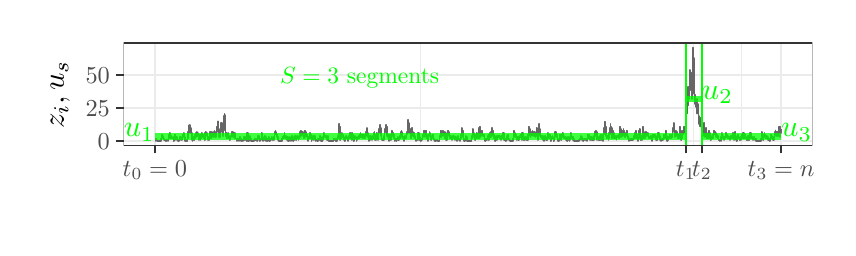
\begin{tikzpicture}[x=1pt,y=1pt]
\definecolor{fillColor}{RGB}{255,255,255}
\path[use as bounding box,fill=fillColor,fill opacity=0.00] (0,0) rectangle (289.08, 72.27);
\begin{scope}
\path[clip] (  0.00,  0.00) rectangle (289.08, 72.27);
\definecolor{drawColor}{RGB}{255,255,255}
\definecolor{fillColor}{RGB}{255,255,255}

\path[draw=drawColor,line width= 0.6pt,line join=round,line cap=round,fill=fillColor] (  0.00,  0.00) rectangle (289.08, 72.27);
\end{scope}
\begin{scope}
\path[clip] ( 34.65, 29.59) rectangle (283.58, 66.77);
\definecolor{fillColor}{RGB}{255,255,255}

\path[fill=fillColor] ( 34.65, 29.59) rectangle (283.58, 66.77);
\definecolor{drawColor}{gray}{0.92}

\path[draw=drawColor,line width= 0.3pt,line join=round] (141.89, 29.59) --
	(141.89, 66.77);

\path[draw=drawColor,line width= 0.3pt,line join=round] (240.71, 29.59) --
	(240.71, 66.77);

\path[draw=drawColor,line width= 0.3pt,line join=round] (257.94, 29.59) --
	(257.94, 66.77);

\path[draw=drawColor,line width= 0.6pt,line join=round] ( 34.65, 31.28) --
	(283.58, 31.28);

\path[draw=drawColor,line width= 0.6pt,line join=round] ( 34.65, 43.18) --
	(283.58, 43.18);

\path[draw=drawColor,line width= 0.6pt,line join=round] ( 34.65, 55.08) --
	(283.58, 55.08);

\path[draw=drawColor,line width= 0.6pt,line join=round] ( 45.97, 29.59) --
	( 45.97, 66.77);

\path[draw=drawColor,line width= 0.6pt,line join=round] (237.82, 29.59) --
	(237.82, 66.77);

\path[draw=drawColor,line width= 0.6pt,line join=round] (243.61, 29.59) --
	(243.61, 66.77);

\path[draw=drawColor,line width= 0.6pt,line join=round] (272.26, 29.59) --
	(272.26, 66.77);
\definecolor{drawColor}{gray}{0.40}

\path[draw=drawColor,line width= 0.6pt,line join=round] ( 45.97, 31.75) --
	( 46.15, 31.75) --
	( 46.15, 31.28) --
	( 46.17, 31.28) --
	( 46.17, 31.75) --
	( 46.18, 31.75) --
	( 46.18, 32.23) --
	( 46.60, 32.23) --
	( 46.60, 31.75) --
	( 46.63, 31.75) --
	( 46.63, 31.28) --
	( 48.22, 31.28) --
	( 48.22, 31.75) --
	( 48.26, 31.75) --
	( 48.26, 32.23) --
	( 48.49, 32.23) --
	( 48.49, 32.71) --
	( 48.56, 32.71) --
	( 48.56, 33.18) --
	( 48.63, 33.18) --
	( 48.63, 33.66) --
	( 48.67, 33.66) --
	( 48.67, 33.18) --
	( 48.71, 33.18) --
	( 48.71, 32.71) --
	( 48.83, 32.71) --
	( 48.83, 33.18) --
	( 48.94, 33.18) --
	( 48.94, 32.71) --
	( 49.00, 32.71) --
	( 49.00, 33.18) --
	( 49.01, 33.18) --
	( 49.01, 32.71) --
	( 49.08, 32.71) --
	( 49.08, 32.23) --
	( 49.29, 32.23) --
	( 49.29, 31.75) --
	( 49.31, 31.75) --
	( 49.31, 32.23) --
	( 49.45, 32.23) --
	( 49.45, 31.75) --
	( 49.76, 31.75) --
	( 49.76, 31.28) --
	( 50.20, 31.28) --
	( 50.20, 31.75) --
	( 50.65, 31.75) --
	( 50.65, 31.28) --
	( 50.68, 31.28) --
	( 50.68, 31.75) --
	( 50.86, 31.75) --
	( 50.86, 32.23) --
	( 50.96, 32.23) --
	( 50.96, 32.71) --
	( 51.04, 32.71) --
	( 51.04, 33.18) --
	( 51.06, 33.18) --
	( 51.06, 33.66) --
	( 51.14, 33.66) --
	( 51.14, 33.18) --
	( 51.20, 33.18) --
	( 51.20, 33.66) --
	( 51.30, 33.66) --
	( 51.30, 34.13) --
	( 51.31, 34.13) --
	( 51.31, 33.66) --
	( 51.32, 33.66) --
	( 51.32, 34.13) --
	( 51.41, 34.13) --
	( 51.41, 33.66) --
	( 51.47, 33.66) --
	( 51.47, 34.13) --
	( 51.50, 34.13) --
	( 51.50, 33.66) --
	( 51.51, 33.66) --
	( 51.51, 33.18) --
	( 51.53, 33.18) --
	( 51.53, 33.66) --
	( 51.65, 33.66) --
	( 51.65, 33.18) --
	( 51.75, 33.18) --
	( 51.75, 32.71) --
	( 51.77, 32.71) --
	( 51.77, 32.23) --
	( 51.80, 32.23) --
	( 51.80, 32.71) --
	( 51.82, 32.71) --
	( 51.82, 33.18) --
	( 51.93, 33.18) --
	( 51.93, 32.71) --
	( 51.97, 32.71) --
	( 51.97, 32.23) --
	( 52.26, 32.23) --
	( 52.26, 32.71) --
	( 52.27, 32.71) --
	( 52.27, 32.23) --
	( 52.70, 32.23) --
	( 52.70, 31.28) --
	( 52.81, 31.28) --
	( 52.81, 31.75) --
	( 52.83, 31.75) --
	( 52.83, 32.23) --
	( 52.88, 32.23) --
	( 52.88, 32.71) --
	( 53.02, 32.71) --
	( 53.02, 33.18) --
	( 53.10, 33.18) --
	( 53.10, 33.66) --
	( 53.26, 33.66) --
	( 53.26, 33.18) --
	( 53.29, 33.18) --
	( 53.29, 32.71) --
	( 53.34, 32.71) --
	( 53.34, 32.23) --
	( 53.34, 32.23) --
	( 53.34, 32.71) --
	( 53.47, 32.71) --
	( 53.47, 32.23) --
	( 53.55, 32.23) --
	( 53.55, 31.75) --
	( 53.60, 31.75) --
	( 53.60, 32.23) --
	( 53.69, 32.23) --
	( 53.69, 32.71) --
	( 53.79, 32.71) --
	( 53.79, 32.23) --
	( 53.98, 32.23) --
	( 53.98, 32.71) --
	( 54.05, 32.71) --
	( 54.05, 32.23) --
	( 54.14, 32.23) --
	( 54.14, 31.75) --
	( 54.43, 31.75) --
	( 54.43, 31.28) --
	( 54.79, 31.28) --
	( 54.79, 31.75) --
	( 55.03, 31.75) --
	( 55.03, 32.23) --
	( 55.09, 32.23) --
	( 55.09, 32.71) --
	( 55.25, 32.71) --
	( 55.25, 32.23) --
	( 55.35, 32.23) --
	( 55.35, 32.71) --
	( 55.48, 32.71) --
	( 55.48, 32.23) --
	( 55.54, 32.23) --
	( 55.54, 31.75) --
	( 55.78, 31.75) --
	( 55.78, 32.23) --
	( 55.80, 32.23) --
	( 55.80, 31.75) --
	( 55.81, 31.75) --
	( 55.81, 32.23) --
	( 55.98, 32.23) --
	( 55.98, 33.18) --
	( 56.17, 33.18) --
	( 56.17, 33.66) --
	( 56.23, 33.66) --
	( 56.23, 33.18) --
	( 56.27, 33.18) --
	( 56.27, 32.71) --
	( 56.41, 32.71) --
	( 56.41, 33.66) --
	( 56.43, 33.66) --
	( 56.43, 34.13) --
	( 56.44, 34.13) --
	( 56.44, 33.18) --
	( 56.62, 33.18) --
	( 56.62, 32.71) --
	( 56.87, 32.71) --
	( 56.87, 31.75) --
	( 56.87, 31.75) --
	( 56.87, 31.28) --
	( 57.13, 31.28) --
	( 57.13, 31.75) --
	( 57.59, 31.75) --
	( 57.59, 31.28) --
	( 57.72, 31.28) --
	( 57.72, 31.75) --
	( 57.77, 31.75) --
	( 57.77, 32.23) --
	( 57.82, 32.23) --
	( 57.82, 33.18) --
	( 57.91, 33.18) --
	( 57.91, 34.13) --
	( 58.05, 34.13) --
	( 58.05, 34.61) --
	( 58.10, 34.61) --
	( 58.10, 35.09) --
	( 58.17, 35.09) --
	( 58.17, 34.61) --
	( 58.20, 34.61) --
	( 58.20, 36.04) --
	( 58.22, 36.04) --
	( 58.22, 36.51) --
	( 58.22, 36.51) --
	( 58.22, 36.04) --
	( 58.27, 36.04) --
	( 58.27, 36.99) --
	( 58.27, 36.99) --
	( 58.27, 36.04) --
	( 58.34, 36.04) --
	( 58.34, 36.51) --
	( 58.37, 36.51) --
	( 58.37, 35.56) --
	( 58.43, 35.56) --
	( 58.43, 36.04) --
	( 58.51, 36.04) --
	( 58.51, 35.56) --
	( 58.56, 35.56) --
	( 58.56, 35.09) --
	( 58.59, 35.09) --
	( 58.59, 36.51) --
	( 58.64, 36.51) --
	( 58.64, 36.99) --
	( 58.65, 36.99) --
	( 58.65, 36.51) --
	( 58.65, 36.51) --
	( 58.65, 35.56) --
	( 58.67, 35.56) --
	( 58.67, 35.09) --
	( 58.73, 35.09) --
	( 58.73, 34.13) --
	( 58.81, 34.13) --
	( 58.81, 34.61) --
	( 58.84, 34.61) --
	( 58.84, 35.09) --
	( 58.84, 35.09) --
	( 58.84, 35.56) --
	( 58.89, 35.56) --
	( 58.89, 35.09) --
	( 58.99, 35.09) --
	( 58.99, 35.56) --
	( 59.02, 35.56) --
	( 59.02, 36.04) --
	( 59.04, 36.04) --
	( 59.04, 34.61) --
	( 59.05, 34.61) --
	( 59.05, 35.09) --
	( 59.09, 35.09) --
	( 59.09, 34.61) --
	( 59.25, 34.61) --
	( 59.25, 34.13) --
	( 59.27, 34.13) --
	( 59.27, 33.66) --
	( 59.29, 33.66) --
	( 59.29, 32.71) --
	( 59.45, 32.71) --
	( 59.45, 31.75) --
	( 59.51, 31.75) --
	( 59.51, 31.28) --
	( 59.56, 31.28) --
	( 59.56, 31.75) --
	( 59.65, 31.75) --
	( 59.65, 32.23) --
	( 59.87, 32.23) --
	( 59.87, 32.71) --
	( 60.00, 32.71) --
	( 60.00, 32.23) --
	( 60.10, 32.23) --
	( 60.10, 31.75) --
	( 60.22, 31.75) --
	( 60.22, 32.23) --
	( 60.32, 32.23) --
	( 60.32, 31.75) --
	( 60.33, 31.75) --
	( 60.33, 32.23) --
	( 60.37, 32.23) --
	( 60.37, 32.71) --
	( 60.39, 32.71) --
	( 60.39, 33.18) --
	( 60.56, 33.18) --
	( 60.56, 33.66) --
	( 60.67, 33.66) --
	( 60.67, 33.18) --
	( 60.69, 33.18) --
	( 60.69, 33.66) --
	( 60.78, 33.66) --
	( 60.78, 33.18) --
	( 60.82, 33.18) --
	( 60.82, 32.71) --
	( 60.83, 32.71) --
	( 60.83, 33.66) --
	( 60.85, 33.66) --
	( 60.85, 33.18) --
	( 60.92, 33.18) --
	( 60.92, 33.66) --
	( 60.94, 33.66) --
	( 60.94, 34.13) --
	( 61.09, 34.13) --
	( 61.09, 34.61) --
	( 61.14, 34.61) --
	( 61.14, 34.13) --
	( 61.23, 34.13) --
	( 61.23, 34.61) --
	( 61.28, 34.61) --
	( 61.28, 33.66) --
	( 61.37, 33.66) --
	( 61.37, 34.13) --
	( 61.38, 34.13) --
	( 61.38, 33.66) --
	( 61.39, 33.66) --
	( 61.39, 33.18) --
	( 61.42, 33.18) --
	( 61.42, 34.13) --
	( 61.46, 34.13) --
	( 61.46, 33.66) --
	( 61.54, 33.66) --
	( 61.54, 33.18) --
	( 61.68, 33.18) --
	( 61.68, 32.71) --
	( 61.79, 32.71) --
	( 61.79, 33.18) --
	( 61.82, 33.18) --
	( 61.82, 32.71) --
	( 61.88, 32.71) --
	( 61.88, 31.75) --
	( 61.89, 31.75) --
	( 61.89, 32.23) --
	( 61.91, 32.23) --
	( 61.91, 32.71) --
	( 61.96, 32.71) --
	( 61.96, 33.18) --
	( 62.22, 33.18) --
	( 62.22, 33.66) --
	( 62.23, 33.66) --
	( 62.23, 33.18) --
	( 62.34, 33.18) --
	( 62.34, 32.71) --
	( 62.36, 32.71) --
	( 62.36, 32.23) --
	( 62.42, 32.23) --
	( 62.42, 31.75) --
	( 62.50, 31.75) --
	( 62.50, 32.23) --
	( 62.61, 32.23) --
	( 62.61, 32.71) --
	( 62.63, 32.71) --
	( 62.63, 33.18) --
	( 62.64, 33.18) --
	( 62.64, 33.66) --
	( 62.66, 33.66) --
	( 62.66, 33.18) --
	( 62.68, 33.18) --
	( 62.68, 33.66) --
	( 62.75, 33.66) --
	( 62.75, 34.13) --
	( 62.95, 34.13) --
	( 62.95, 33.66) --
	( 63.03, 33.66) --
	( 63.03, 34.13) --
	( 63.09, 34.13) --
	( 63.09, 33.66) --
	( 63.09, 33.66) --
	( 63.09, 33.18) --
	( 63.10, 33.18) --
	( 63.10, 33.66) --
	( 63.14, 33.66) --
	( 63.14, 33.18) --
	( 63.20, 33.18) --
	( 63.20, 32.71) --
	( 63.42, 32.71) --
	( 63.42, 33.18) --
	( 63.45, 33.18) --
	( 63.45, 33.66) --
	( 63.48, 33.66) --
	( 63.48, 33.18) --
	( 63.51, 33.18) --
	( 63.51, 32.71) --
	( 63.55, 32.71) --
	( 63.55, 32.23) --
	( 63.86, 32.23) --
	( 63.86, 32.71) --
	( 63.87, 32.71) --
	( 63.87, 32.23) --
	( 63.91, 32.23) --
	( 63.91, 31.75) --
	( 63.96, 31.75) --
	( 63.96, 32.23) --
	( 63.97, 32.23) --
	( 63.97, 32.71) --
	( 64.06, 32.71) --
	( 64.06, 33.18) --
	( 64.14, 33.18) --
	( 64.14, 33.66) --
	( 64.17, 33.66) --
	( 64.17, 34.13) --
	( 64.25, 34.13) --
	( 64.25, 34.61) --
	( 64.31, 34.61) --
	( 64.31, 34.13) --
	( 64.39, 34.13) --
	( 64.39, 34.61) --
	( 64.41, 34.61) --
	( 64.41, 34.13) --
	( 64.42, 34.13) --
	( 64.42, 33.66) --
	( 64.48, 33.66) --
	( 64.48, 33.18) --
	( 64.52, 33.18) --
	( 64.52, 33.66) --
	( 64.58, 33.66) --
	( 64.58, 34.13) --
	( 64.59, 34.13) --
	( 64.59, 33.66) --
	( 64.60, 33.66) --
	( 64.60, 34.13) --
	( 64.62, 34.13) --
	( 64.62, 33.66) --
	( 64.65, 33.66) --
	( 64.65, 34.13) --
	( 64.71, 34.13) --
	( 64.71, 33.66) --
	( 64.76, 33.66) --
	( 64.76, 34.13) --
	( 64.85, 34.13) --
	( 64.85, 33.66) --
	( 64.97, 33.66) --
	( 64.97, 33.18) --
	( 65.04, 33.18) --
	( 65.04, 32.71) --
	( 65.05, 32.71) --
	( 65.05, 32.23) --
	( 65.10, 32.23) --
	( 65.10, 31.75) --
	( 65.13, 31.75) --
	( 65.13, 32.23) --
	( 65.15, 32.23) --
	( 65.15, 31.75) --
	( 65.28, 31.75) --
	( 65.28, 32.23) --
	( 65.53, 32.23) --
	( 65.53, 32.71) --
	( 65.58, 32.71) --
	( 65.58, 32.23) --
	( 65.73, 32.23) --
	( 65.73, 31.75) --
	( 65.76, 31.75) --
	( 65.76, 32.71) --
	( 65.78, 32.71) --
	( 65.78, 33.18) --
	( 65.80, 33.18) --
	( 65.80, 33.66) --
	( 65.82, 33.66) --
	( 65.82, 34.13) --
	( 65.86, 34.13) --
	( 65.86, 34.61) --
	( 65.98, 34.61) --
	( 65.98, 34.13) --
	( 66.05, 34.13) --
	( 66.05, 34.61) --
	( 66.21, 34.61) --
	( 66.21, 33.66) --
	( 66.24, 33.66) --
	( 66.24, 33.18) --
	( 66.24, 33.18) --
	( 66.24, 32.71) --
	( 66.31, 32.71) --
	( 66.31, 32.23) --
	( 66.39, 32.23) --
	( 66.39, 32.71) --
	( 66.41, 32.71) --
	( 66.41, 33.66) --
	( 66.53, 33.66) --
	( 66.53, 34.13) --
	( 66.58, 34.13) --
	( 66.58, 34.61) --
	( 66.72, 34.61) --
	( 66.72, 34.13) --
	( 66.84, 34.13) --
	( 66.84, 33.66) --
	( 66.86, 33.66) --
	( 66.86, 32.71) --
	( 66.89, 32.71) --
	( 66.89, 33.18) --
	( 66.96, 33.18) --
	( 66.96, 32.71) --
	( 66.98, 32.71) --
	( 66.98, 33.18) --
	( 66.99, 33.18) --
	( 66.99, 32.71) --
	( 67.02, 32.71) --
	( 67.02, 33.18) --
	( 67.03, 33.18) --
	( 67.03, 32.71) --
	( 67.09, 32.71) --
	( 67.09, 33.18) --
	( 67.16, 33.18) --
	( 67.16, 33.66) --
	( 67.19, 33.66) --
	( 67.19, 34.13) --
	( 67.27, 34.13) --
	( 67.27, 34.61) --
	( 67.34, 34.61) --
	( 67.34, 34.13) --
	( 67.34, 34.13) --
	( 67.34, 34.61) --
	( 67.43, 34.61) --
	( 67.43, 34.13) --
	( 67.46, 34.13) --
	( 67.46, 34.61) --
	( 67.47, 34.61) --
	( 67.47, 35.09) --
	( 67.48, 35.09) --
	( 67.48, 34.61) --
	( 67.54, 34.61) --
	( 67.54, 34.13) --
	( 67.62, 34.13) --
	( 67.62, 33.66) --
	( 67.64, 33.66) --
	( 67.64, 33.18) --
	( 67.72, 33.18) --
	( 67.72, 32.71) --
	( 67.73, 32.71) --
	( 67.73, 33.18) --
	( 67.76, 33.18) --
	( 67.76, 34.13) --
	( 67.80, 34.13) --
	( 67.80, 33.66) --
	( 67.91, 33.66) --
	( 67.91, 33.18) --
	( 67.92, 33.18) --
	( 67.92, 32.71) --
	( 67.94, 32.71) --
	( 67.94, 33.18) --
	( 67.99, 33.18) --
	( 67.99, 33.66) --
	( 68.06, 33.66) --
	( 68.06, 34.13) --
	( 68.16, 34.13) --
	( 68.16, 34.61) --
	( 68.18, 34.61) --
	( 68.18, 34.13) --
	( 68.20, 34.13) --
	( 68.20, 34.61) --
	( 68.20, 34.61) --
	( 68.20, 35.09) --
	( 68.21, 35.09) --
	( 68.21, 34.61) --
	( 68.21, 34.61) --
	( 68.21, 34.13) --
	( 68.24, 34.13) --
	( 68.24, 34.61) --
	( 68.39, 34.61) --
	( 68.39, 35.09) --
	( 68.39, 35.09) --
	( 68.39, 34.61) --
	( 68.44, 34.61) --
	( 68.44, 35.09) --
	( 68.44, 35.09) --
	( 68.44, 34.61) --
	( 68.46, 34.61) --
	( 68.46, 36.04) --
	( 68.47, 36.04) --
	( 68.47, 36.51) --
	( 68.49, 36.51) --
	( 68.49, 36.04) --
	( 68.51, 36.04) --
	( 68.51, 36.51) --
	( 68.56, 36.51) --
	( 68.56, 36.99) --
	( 68.60, 36.99) --
	( 68.60, 37.47) --
	( 68.61, 37.47) --
	( 68.61, 36.99) --
	( 68.65, 36.99) --
	( 68.65, 36.51) --
	( 68.66, 36.51) --
	( 68.66, 36.04) --
	( 68.66, 36.04) --
	( 68.66, 36.51) --
	( 68.69, 36.51) --
	( 68.69, 36.99) --
	( 68.69, 36.99) --
	( 68.69, 36.51) --
	( 68.70, 36.51) --
	( 68.70, 37.47) --
	( 68.77, 37.47) --
	( 68.77, 37.94) --
	( 68.83, 37.94) --
	( 68.83, 38.42) --
	( 68.83, 38.42) --
	( 68.83, 37.94) --
	( 68.89, 37.94) --
	( 68.89, 37.47) --
	( 68.92, 37.47) --
	( 68.92, 36.04) --
	( 68.92, 36.04) --
	( 68.92, 35.09) --
	( 68.93, 35.09) --
	( 68.93, 35.56) --
	( 68.99, 35.56) --
	( 68.99, 36.04) --
	( 69.01, 36.04) --
	( 69.01, 35.56) --
	( 69.05, 35.56) --
	( 69.05, 35.09) --
	( 69.06, 35.09) --
	( 69.06, 34.61) --
	( 69.14, 34.61) --
	( 69.14, 34.13) --
	( 69.16, 34.13) --
	( 69.16, 33.18) --
	( 69.20, 33.18) --
	( 69.20, 33.66) --
	( 69.21, 33.66) --
	( 69.21, 32.71) --
	( 69.30, 32.71) --
	( 69.30, 33.18) --
	( 69.38, 33.18) --
	( 69.38, 33.66) --
	( 69.39, 33.66) --
	( 69.39, 33.18) --
	( 69.44, 33.18) --
	( 69.44, 32.71) --
	( 69.51, 32.71) --
	( 69.51, 33.66) --
	( 69.55, 33.66) --
	( 69.55, 34.13) --
	( 69.59, 34.13) --
	( 69.59, 34.61) --
	( 69.59, 34.61) --
	( 69.59, 34.13) --
	( 69.66, 34.13) --
	( 69.66, 34.61) --
	( 69.68, 34.61) --
	( 69.68, 35.09) --
	( 69.75, 35.09) --
	( 69.75, 34.61) --
	( 69.78, 34.61) --
	( 69.78, 35.09) --
	( 69.79, 35.09) --
	( 69.79, 35.56) --
	( 69.82, 35.56) --
	( 69.82, 36.04) --
	( 69.85, 36.04) --
	( 69.85, 35.56) --
	( 69.87, 35.56) --
	( 69.87, 36.04) --
	( 69.90, 36.04) --
	( 69.90, 36.51) --
	( 69.92, 36.51) --
	( 69.92, 36.99) --
	( 69.92, 36.99) --
	( 69.92, 37.47) --
	( 69.97, 37.47) --
	( 69.97, 37.94) --
	( 70.00, 37.94) --
	( 70.00, 37.47) --
	( 70.02, 37.47) --
	( 70.02, 37.94) --
	( 70.04, 37.94) --
	( 70.04, 37.47) --
	( 70.05, 37.47) --
	( 70.05, 36.99) --
	( 70.08, 36.99) --
	( 70.08, 37.47) --
	( 70.09, 37.47) --
	( 70.09, 37.94) --
	( 70.11, 37.94) --
	( 70.11, 37.47) --
	( 70.19, 37.47) --
	( 70.19, 37.94) --
	( 70.24, 37.94) --
	( 70.24, 37.47) --
	( 70.27, 37.47) --
	( 70.27, 36.99) --
	( 70.28, 36.99) --
	( 70.28, 37.47) --
	( 70.29, 37.47) --
	( 70.29, 36.99) --
	( 70.32, 36.99) --
	( 70.32, 37.47) --
	( 70.35, 37.47) --
	( 70.35, 36.99) --
	( 70.37, 36.99) --
	( 70.37, 36.51) --
	( 70.38, 36.51) --
	( 70.38, 36.04) --
	( 70.41, 36.04) --
	( 70.41, 35.56) --
	( 70.43, 35.56) --
	( 70.43, 35.09) --
	( 70.47, 35.09) --
	( 70.47, 34.61) --
	( 70.52, 34.61) --
	( 70.52, 34.13) --
	( 70.53, 34.13) --
	( 70.53, 34.61) --
	( 70.54, 34.61) --
	( 70.54, 34.13) --
	( 70.54, 34.13) --
	( 70.54, 33.66) --
	( 70.59, 33.66) --
	( 70.59, 33.18) --
	( 70.60, 33.18) --
	( 70.60, 33.66) --
	( 70.63, 33.66) --
	( 70.63, 34.13) --
	( 70.64, 34.13) --
	( 70.64, 33.66) --
	( 70.72, 33.66) --
	( 70.72, 34.13) --
	( 70.73, 34.13) --
	( 70.73, 33.66) --
	( 70.77, 33.66) --
	( 70.77, 33.18) --
	( 70.79, 33.18) --
	( 70.79, 33.66) --
	( 70.79, 33.66) --
	( 70.79, 34.61) --
	( 70.80, 34.61) --
	( 70.80, 35.09) --
	( 70.86, 35.09) --
	( 70.86, 35.56) --
	( 70.89, 35.56) --
	( 70.89, 36.04) --
	( 70.91, 36.04) --
	( 70.91, 36.51) --
	( 70.91, 36.51) --
	( 70.91, 36.99) --
	( 70.95, 36.99) --
	( 70.95, 37.47) --
	( 70.97, 37.47) --
	( 70.97, 37.94) --
	( 70.98, 37.94) --
	( 70.98, 37.47) --
	( 70.98, 37.47) --
	( 70.98, 37.94) --
	( 71.00, 37.94) --
	( 71.00, 39.37) --
	( 71.02, 39.37) --
	( 71.02, 39.85) --
	( 71.04, 39.85) --
	( 71.04, 39.37) --
	( 71.05, 39.37) --
	( 71.05, 39.85) --
	( 71.06, 39.85) --
	( 71.06, 40.32) --
	( 71.07, 40.32) --
	( 71.07, 40.80) --
	( 71.08, 40.80) --
	( 71.08, 41.27) --
	( 71.09, 41.27) --
	( 71.09, 40.80) --
	( 71.14, 40.80) --
	( 71.14, 41.27) --
	( 71.17, 41.27) --
	( 71.17, 40.80) --
	( 71.24, 40.80) --
	( 71.24, 40.32) --
	( 71.25, 40.32) --
	( 71.25, 39.85) --
	( 71.26, 39.85) --
	( 71.26, 39.37) --
	( 71.31, 39.37) --
	( 71.31, 38.89) --
	( 71.35, 38.89) --
	( 71.35, 38.42) --
	( 71.36, 38.42) --
	( 71.36, 37.94) --
	( 71.36, 37.94) --
	( 71.36, 37.47) --
	( 71.40, 37.47) --
	( 71.40, 36.99) --
	( 71.42, 36.99) --
	( 71.42, 36.51) --
	( 71.44, 36.51) --
	( 71.44, 36.04) --
	( 71.45, 36.04) --
	( 71.45, 34.61) --
	( 71.46, 34.61) --
	( 71.46, 35.09) --
	( 71.47, 35.09) --
	( 71.47, 34.13) --
	( 71.50, 34.13) --
	( 71.50, 33.66) --
	( 71.51, 33.66) --
	( 71.51, 33.18) --
	( 71.52, 33.18) --
	( 71.52, 33.66) --
	( 71.53, 33.66) --
	( 71.53, 34.13) --
	( 71.54, 34.13) --
	( 71.54, 33.66) --
	( 71.59, 33.66) --
	( 71.59, 33.18) --
	( 71.71, 33.18) --
	( 71.71, 34.13) --
	( 71.91, 34.13) --
	( 71.91, 33.66) --
	( 71.97, 33.66) --
	( 71.97, 32.23) --
	( 72.14, 32.23) --
	( 72.14, 33.18) --
	( 72.16, 33.18) --
	( 72.16, 32.23) --
	( 72.25, 32.23) --
	( 72.25, 32.71) --
	( 72.38, 32.71) --
	( 72.38, 33.18) --
	( 72.52, 33.18) --
	( 72.52, 33.66) --
	( 72.53, 33.66) --
	( 72.53, 34.13) --
	( 72.59, 34.13) --
	( 72.59, 33.18) --
	( 72.69, 33.18) --
	( 72.69, 32.71) --
	( 72.83, 32.71) --
	( 72.83, 32.23) --
	( 72.84, 32.23) --
	( 72.84, 32.71) --
	( 72.97, 32.71) --
	( 72.97, 32.23) --
	( 72.98, 32.23) --
	( 72.98, 31.75) --
	( 73.00, 31.75) --
	( 73.00, 32.23) --
	( 73.01, 32.23) --
	( 73.01, 32.71) --
	( 73.28, 32.71) --
	( 73.28, 33.18) --
	( 73.29, 33.18) --
	( 73.29, 32.71) --
	( 73.43, 32.71) --
	( 73.43, 33.18) --
	( 73.46, 33.18) --
	( 73.46, 32.71) --
	( 73.53, 32.71) --
	( 73.53, 33.18) --
	( 73.66, 33.18) --
	( 73.66, 33.66) --
	( 73.73, 33.66) --
	( 73.73, 33.18) --
	( 73.77, 33.18) --
	( 73.77, 33.66) --
	( 73.83, 33.66) --
	( 73.83, 34.61) --
	( 73.88, 34.61) --
	( 73.88, 34.13) --
	( 73.91, 34.13) --
	( 73.91, 33.66) --
	( 73.98, 33.66) --
	( 73.98, 33.18) --
	( 74.03, 33.18) --
	( 74.03, 33.66) --
	( 74.05, 33.66) --
	( 74.05, 34.13) --
	( 74.11, 34.13) --
	( 74.11, 33.66) --
	( 74.16, 33.66) --
	( 74.16, 34.13) --
	( 74.20, 34.13) --
	( 74.20, 34.61) --
	( 74.21, 34.61) --
	( 74.21, 34.13) --
	( 74.21, 34.13) --
	( 74.21, 33.66) --
	( 74.24, 33.66) --
	( 74.24, 33.18) --
	( 74.28, 33.18) --
	( 74.28, 32.71) --
	( 74.36, 32.71) --
	( 74.36, 33.18) --
	( 74.38, 33.18) --
	( 74.38, 33.66) --
	( 74.41, 33.66) --
	( 74.41, 33.18) --
	( 74.50, 33.18) --
	( 74.50, 32.71) --
	( 74.52, 32.71) --
	( 74.52, 33.18) --
	( 74.52, 33.18) --
	( 74.52, 33.66) --
	( 74.62, 33.66) --
	( 74.62, 34.13) --
	( 74.65, 34.13) --
	( 74.65, 33.66) --
	( 74.65, 33.66) --
	( 74.65, 34.13) --
	( 74.81, 34.13) --
	( 74.81, 33.66) --
	( 74.83, 33.66) --
	( 74.83, 33.18) --
	( 74.97, 33.18) --
	( 74.97, 32.23) --
	( 75.05, 32.23) --
	( 75.05, 32.71) --
	( 75.07, 32.71) --
	( 75.07, 32.23) --
	( 75.08, 32.23) --
	( 75.08, 32.71) --
	( 75.10, 32.71) --
	( 75.10, 32.23) --
	( 75.50, 32.23) --
	( 75.50, 31.75) --
	( 75.53, 31.75) --
	( 75.53, 31.28) --
	( 75.72, 31.28) --
	( 75.72, 31.75) --
	( 75.83, 31.75) --
	( 75.83, 32.23) --
	( 76.12, 32.23) --
	( 76.12, 31.75) --
	( 76.28, 31.75) --
	( 76.28, 31.28) --
	( 76.47, 31.28) --
	( 76.47, 31.75) --
	( 76.53, 31.75) --
	( 76.53, 32.23) --
	( 76.54, 32.23) --
	( 76.54, 32.71) --
	( 76.92, 32.71) --
	( 76.92, 32.23) --
	( 76.98, 32.23) --
	( 76.98, 31.75) --
	( 76.99, 31.75) --
	( 76.99, 31.28) --
	( 77.22, 31.28) --
	( 77.22, 31.75) --
	( 77.68, 31.75) --
	( 77.68, 31.28) --
	( 77.89, 31.28) --
	( 77.89, 31.75) --
	( 78.03, 31.75) --
	( 78.03, 32.23) --
	( 78.20, 32.23) --
	( 78.20, 32.71) --
	( 78.24, 32.71) --
	( 78.24, 32.23) --
	( 78.35, 32.23) --
	( 78.35, 31.75) --
	( 78.51, 31.75) --
	( 78.51, 32.23) --
	( 78.57, 32.23) --
	( 78.57, 32.71) --
	( 78.65, 32.71) --
	( 78.65, 32.23) --
	( 78.96, 32.23) --
	( 78.96, 31.75) --
	( 79.02, 31.75) --
	( 79.02, 31.28) --
	( 79.20, 31.28) --
	( 79.20, 32.71) --
	( 79.23, 32.71) --
	( 79.23, 34.13) --
	( 79.65, 34.13) --
	( 79.65, 32.71) --
	( 79.68, 32.71) --
	( 79.68, 32.23) --
	( 79.68, 32.23) --
	( 79.68, 31.28) --
	( 79.93, 31.28) --
	( 79.93, 31.75) --
	( 79.96, 31.75) --
	( 79.96, 32.23) --
	( 80.14, 32.23) --
	( 80.14, 32.71) --
	( 80.29, 32.71) --
	( 80.29, 33.18) --
	( 80.35, 33.18) --
	( 80.35, 32.71) --
	( 80.41, 32.71) --
	( 80.41, 32.23) --
	( 80.59, 32.23) --
	( 80.59, 31.75) --
	( 80.74, 31.75) --
	( 80.74, 31.28) --
	( 81.79, 31.28) --
	( 81.79, 31.75) --
	( 82.03, 31.75) --
	( 82.03, 32.23) --
	( 82.24, 32.23) --
	( 82.24, 31.75) --
	( 82.27, 31.75) --
	( 82.27, 32.23) --
	( 82.48, 32.23) --
	( 82.48, 31.75) --
	( 82.53, 31.75) --
	( 82.53, 32.23) --
	( 82.72, 32.23) --
	( 82.72, 31.75) --
	( 82.98, 31.75) --
	( 82.98, 31.28) --
	( 83.02, 31.28) --
	( 83.02, 31.75) --
	( 83.25, 31.75) --
	( 83.25, 32.23) --
	( 83.28, 32.23) --
	( 83.28, 32.71) --
	( 83.29, 32.71) --
	( 83.29, 33.18) --
	( 83.47, 33.18) --
	( 83.47, 32.71) --
	( 83.71, 32.71) --
	( 83.71, 32.23) --
	( 83.73, 32.23) --
	( 83.73, 31.75) --
	( 83.74, 31.75) --
	( 83.74, 31.28) --
	( 83.85, 31.28) --
	( 83.85, 31.75) --
	( 84.23, 31.75) --
	( 84.23, 32.23) --
	( 84.30, 32.23) --
	( 84.30, 31.75) --
	( 84.38, 31.75) --
	( 84.38, 32.23) --
	( 84.46, 32.23) --
	( 84.46, 32.71) --
	( 84.49, 32.71) --
	( 84.49, 33.66) --
	( 84.51, 33.66) --
	( 84.51, 34.13) --
	( 84.68, 34.13) --
	( 84.68, 33.66) --
	( 84.83, 33.66) --
	( 84.83, 33.18) --
	( 84.91, 33.18) --
	( 84.91, 32.71) --
	( 84.95, 32.71) --
	( 84.95, 31.75) --
	( 84.96, 31.75) --
	( 84.96, 31.28) --
	( 84.99, 31.28) --
	( 84.99, 31.75) --
	( 85.22, 31.75) --
	( 85.22, 32.23) --
	( 85.44, 32.23) --
	( 85.44, 31.75) --
	( 85.57, 31.75) --
	( 85.57, 32.23) --
	( 85.63, 32.23) --
	( 85.63, 33.18) --
	( 85.67, 33.18) --
	( 85.67, 32.71) --
	( 86.02, 32.71) --
	( 86.02, 32.23) --
	( 86.08, 32.23) --
	( 86.08, 31.28) --
	( 86.14, 31.28) --
	( 86.14, 31.75) --
	( 86.38, 31.75) --
	( 86.38, 32.23) --
	( 86.59, 32.23) --
	( 86.59, 31.28) --
	( 86.66, 31.28) --
	( 86.66, 31.75) --
	( 86.80, 31.75) --
	( 86.80, 32.23) --
	( 87.05, 32.23) --
	( 87.05, 32.71) --
	( 87.09, 32.71) --
	( 87.09, 32.23) --
	( 87.24, 32.23) --
	( 87.24, 31.28) --
	( 87.50, 31.28) --
	( 87.50, 31.75) --
	( 87.93, 31.75) --
	( 87.93, 32.23) --
	( 87.95, 32.23) --
	( 87.95, 31.75) --
	( 88.03, 31.75) --
	( 88.03, 32.23) --
	( 88.20, 32.23) --
	( 88.20, 32.71) --
	( 88.38, 32.71) --
	( 88.38, 32.23) --
	( 88.49, 32.23) --
	( 88.49, 31.75) --
	( 88.50, 31.75) --
	( 88.50, 32.23) --
	( 88.63, 32.23) --
	( 88.63, 31.75) --
	( 88.76, 31.75) --
	( 88.76, 32.23) --
	( 88.95, 32.23) --
	( 88.95, 31.75) --
	( 89.11, 31.75) --
	( 89.11, 32.23) --
	( 89.12, 32.23) --
	( 89.12, 32.71) --
	( 89.17, 32.71) --
	( 89.17, 33.66) --
	( 89.21, 33.66) --
	( 89.21, 33.18) --
	( 89.25, 33.18) --
	( 89.25, 33.66) --
	( 89.28, 33.66) --
	( 89.28, 34.13) --
	( 89.39, 34.13) --
	( 89.39, 34.61) --
	( 89.50, 34.61) --
	( 89.50, 35.09) --
	( 89.56, 35.09) --
	( 89.56, 34.61) --
	( 89.57, 34.61) --
	( 89.57, 35.09) --
	( 89.58, 35.09) --
	( 89.58, 34.61) --
	( 89.63, 34.61) --
	( 89.63, 33.66) --
	( 89.69, 33.66) --
	( 89.69, 34.13) --
	( 89.70, 34.13) --
	( 89.70, 33.66) --
	( 89.71, 33.66) --
	( 89.71, 34.13) --
	( 89.73, 34.13) --
	( 89.73, 33.66) --
	( 89.81, 33.66) --
	( 89.81, 34.13) --
	( 89.84, 34.13) --
	( 89.84, 33.66) --
	( 89.95, 33.66) --
	( 89.95, 33.18) --
	( 89.99, 33.18) --
	( 89.99, 33.66) --
	( 90.02, 33.66) --
	( 90.02, 33.18) --
	( 90.08, 33.18) --
	( 90.08, 33.66) --
	( 90.15, 33.66) --
	( 90.15, 33.18) --
	( 90.15, 33.18) --
	( 90.15, 32.71) --
	( 90.22, 32.71) --
	( 90.22, 33.18) --
	( 90.26, 33.18) --
	( 90.26, 32.71) --
	( 90.44, 32.71) --
	( 90.44, 32.23) --
	( 90.54, 32.23) --
	( 90.54, 31.75) --
	( 90.68, 31.75) --
	( 90.68, 31.28) --
	( 91.91, 31.28) --
	( 91.91, 31.75) --
	( 91.93, 31.75) --
	( 91.93, 32.23) --
	( 92.07, 32.23) --
	( 92.07, 32.71) --
	( 92.35, 32.71) --
	( 92.35, 32.23) --
	( 92.36, 32.23) --
	( 92.36, 32.71) --
	( 92.38, 32.71) --
	( 92.38, 33.18) --
	( 92.39, 33.18) --
	( 92.39, 32.71) --
	( 92.53, 32.71) --
	( 92.53, 32.23) --
	( 92.61, 32.23) --
	( 92.61, 32.71) --
	( 92.69, 32.71) --
	( 92.69, 33.18) --
	( 92.79, 33.18) --
	( 92.79, 34.13) --
	( 92.81, 34.13) --
	( 92.81, 33.66) --
	( 92.83, 33.66) --
	( 92.83, 33.18) --
	( 93.07, 33.18) --
	( 93.07, 32.71) --
	( 93.11, 32.71) --
	( 93.11, 33.18) --
	( 93.14, 33.18) --
	( 93.14, 32.71) --
	( 93.16, 32.71) --
	( 93.16, 33.18) --
	( 93.24, 33.18) --
	( 93.24, 32.23) --
	( 93.52, 32.23) --
	( 93.52, 32.71) --
	( 93.56, 32.71) --
	( 93.56, 32.23) --
	( 93.61, 32.23) --
	( 93.61, 31.75) --
	( 93.64, 31.75) --
	( 93.64, 32.23) --
	( 93.72, 32.23) --
	( 93.72, 32.71) --
	( 93.97, 32.71) --
	( 93.97, 32.23) --
	( 94.09, 32.23) --
	( 94.09, 31.75) --
	( 94.17, 31.75) --
	( 94.17, 31.28) --
	( 94.42, 31.28) --
	( 94.42, 31.75) --
	( 94.42, 31.75) --
	( 94.42, 32.23) --
	( 94.75, 32.23) --
	( 94.75, 32.71) --
	( 94.87, 32.71) --
	( 94.87, 31.75) --
	( 95.20, 31.75) --
	( 95.20, 31.28) --
	( 95.22, 31.28) --
	( 95.22, 31.75) --
	( 95.39, 31.75) --
	( 95.39, 32.23) --
	( 95.47, 32.23) --
	( 95.47, 32.71) --
	( 95.50, 32.71) --
	( 95.50, 33.18) --
	( 95.67, 33.18) --
	( 95.67, 32.71) --
	( 95.84, 32.71) --
	( 95.84, 32.23) --
	( 95.92, 32.23) --
	( 95.92, 31.75) --
	( 95.95, 31.75) --
	( 95.95, 31.28) --
	( 96.00, 31.28) --
	( 96.00, 31.75) --
	( 96.37, 31.75) --
	( 96.37, 32.23) --
	( 96.44, 32.23) --
	( 96.44, 32.71) --
	( 96.45, 32.71) --
	( 96.45, 32.23) --
	( 96.46, 32.23) --
	( 96.46, 32.71) --
	( 96.56, 32.71) --
	( 96.56, 33.18) --
	( 96.82, 33.18) --
	( 96.82, 32.71) --
	( 96.84, 32.71) --
	( 96.84, 33.18) --
	( 96.89, 33.18) --
	( 96.89, 32.71) --
	( 96.90, 32.71) --
	( 96.90, 32.23) --
	( 97.01, 32.23) --
	( 97.01, 31.75) --
	( 97.14, 31.75) --
	( 97.14, 32.23) --
	( 97.22, 32.23) --
	( 97.22, 32.71) --
	( 97.30, 32.71) --
	( 97.30, 32.23) --
	( 97.36, 32.23) --
	( 97.36, 32.71) --
	( 97.44, 32.71) --
	( 97.44, 33.18) --
	( 97.58, 33.18) --
	( 97.58, 32.71) --
	( 97.60, 32.71) --
	( 97.60, 33.18) --
	( 97.67, 33.18) --
	( 97.67, 32.71) --
	( 97.81, 32.71) --
	( 97.81, 32.23) --
	( 97.89, 32.23) --
	( 97.89, 31.75) --
	( 97.92, 31.75) --
	( 97.92, 32.23) --
	( 97.95, 32.23) --
	( 97.95, 32.71) --
	( 98.06, 32.71) --
	( 98.06, 32.23) --
	( 98.11, 32.23) --
	( 98.11, 32.71) --
	( 98.19, 32.71) --
	( 98.19, 32.23) --
	( 98.21, 32.23) --
	( 98.21, 32.71) --
	( 98.32, 32.71) --
	( 98.32, 33.18) --
	( 98.36, 33.18) --
	( 98.36, 33.66) --
	( 98.42, 33.66) --
	( 98.42, 34.13) --
	( 98.51, 34.13) --
	( 98.51, 34.61) --
	( 98.56, 34.61) --
	( 98.56, 34.13) --
	( 98.65, 34.13) --
	( 98.65, 33.66) --
	( 98.70, 33.66) --
	( 98.70, 34.13) --
	( 98.70, 34.13) --
	( 98.70, 34.61) --
	( 98.76, 34.61) --
	( 98.76, 35.09) --
	( 98.77, 35.09) --
	( 98.77, 34.61) --
	( 98.81, 34.61) --
	( 98.81, 34.13) --
	( 98.84, 34.13) --
	( 98.84, 34.61) --
	( 98.85, 34.61) --
	( 98.85, 33.66) --
	( 98.96, 33.66) --
	( 98.96, 33.18) --
	( 98.96, 33.18) --
	( 98.96, 33.66) --
	( 99.12, 33.66) --
	( 99.12, 34.13) --
	( 99.15, 34.13) --
	( 99.15, 33.66) --
	( 99.16, 33.66) --
	( 99.16, 33.18) --
	( 99.16, 33.18) --
	( 99.16, 33.66) --
	( 99.19, 33.66) --
	( 99.19, 34.13) --
	( 99.21, 34.13) --
	( 99.21, 34.61) --
	( 99.22, 34.61) --
	( 99.22, 34.13) --
	( 99.25, 34.13) --
	( 99.25, 34.61) --
	( 99.29, 34.61) --
	( 99.29, 34.13) --
	( 99.39, 34.13) --
	( 99.39, 34.61) --
	( 99.41, 34.61) --
	( 99.41, 34.13) --
	( 99.50, 34.13) --
	( 99.50, 34.61) --
	( 99.57, 34.61) --
	( 99.57, 34.13) --
	( 99.61, 34.13) --
	( 99.61, 33.66) --
	( 99.64, 33.66) --
	( 99.64, 33.18) --
	( 99.65, 33.18) --
	( 99.65, 33.66) --
	( 99.70, 33.66) --
	( 99.70, 33.18) --
	( 99.84, 33.18) --
	( 99.84, 32.71) --
	( 99.86, 32.71) --
	( 99.86, 32.23) --
	( 99.89, 32.23) --
	( 99.89, 32.71) --
	( 99.89, 32.71) --
	( 99.89, 33.18) --
	(100.10, 33.18) --
	(100.10, 32.71) --
	(100.18, 32.71) --
	(100.18, 33.18) --
	(100.24, 33.18) --
	(100.24, 33.66) --
	(100.26, 33.66) --
	(100.26, 34.13) --
	(100.32, 34.13) --
	(100.32, 35.09) --
	(100.34, 35.09) --
	(100.34, 34.61) --
	(100.34, 34.61) --
	(100.34, 34.13) --
	(100.38, 34.13) --
	(100.38, 34.61) --
	(100.40, 34.61) --
	(100.40, 34.13) --
	(100.49, 34.13) --
	(100.49, 34.61) --
	(100.63, 34.61) --
	(100.63, 34.13) --
	(100.68, 34.13) --
	(100.68, 33.66) --
	(100.71, 33.66) --
	(100.71, 33.18) --
	(100.74, 33.18) --
	(100.74, 34.13) --
	(100.77, 34.13) --
	(100.77, 33.66) --
	(100.77, 33.66) --
	(100.77, 33.18) --
	(100.78, 33.18) --
	(100.78, 33.66) --
	(100.83, 33.66) --
	(100.83, 33.18) --
	(100.94, 33.18) --
	(100.94, 32.71) --
	(101.19, 32.71) --
	(101.19, 31.75) --
	(101.23, 31.75) --
	(101.23, 31.28) --
	(101.29, 31.28) --
	(101.29, 31.75) --
	(101.52, 31.75) --
	(101.52, 32.23) --
	(101.68, 32.23) --
	(101.68, 32.71) --
	(101.75, 32.71) --
	(101.75, 32.23) --
	(101.93, 32.23) --
	(101.93, 33.18) --
	(101.97, 33.18) --
	(101.97, 32.71) --
	(101.98, 32.71) --
	(101.98, 33.66) --
	(102.05, 33.66) --
	(102.05, 34.13) --
	(102.14, 34.13) --
	(102.14, 33.66) --
	(102.16, 33.66) --
	(102.16, 33.18) --
	(102.19, 33.18) --
	(102.19, 33.66) --
	(102.38, 33.66) --
	(102.38, 33.18) --
	(102.43, 33.18) --
	(102.43, 32.71) --
	(102.43, 32.71) --
	(102.43, 32.23) --
	(102.51, 32.23) --
	(102.51, 31.28) --
	(102.51, 31.28) --
	(102.51, 31.75) --
	(102.68, 31.75) --
	(102.68, 32.23) --
	(102.81, 32.23) --
	(102.81, 32.71) --
	(102.85, 32.71) --
	(102.85, 33.18) --
	(102.96, 33.18) --
	(102.96, 32.71) --
	(103.14, 32.71) --
	(103.14, 32.23) --
	(103.26, 32.23) --
	(103.26, 31.75) --
	(103.29, 31.75) --
	(103.29, 32.23) --
	(103.33, 32.23) --
	(103.33, 32.71) --
	(103.55, 32.71) --
	(103.55, 33.18) --
	(103.75, 33.18) --
	(103.75, 32.71) --
	(103.76, 32.71) --
	(103.76, 32.23) --
	(103.78, 32.23) --
	(103.78, 31.75) --
	(104.00, 31.75) --
	(104.00, 31.28) --
	(104.01, 31.28) --
	(104.01, 31.75) --
	(104.47, 31.75) --
	(104.47, 31.28) --
	(104.81, 31.28) --
	(104.81, 31.75) --
	(105.00, 31.75) --
	(105.00, 32.23) --
	(105.13, 32.23) --
	(105.13, 31.75) --
	(105.41, 31.75) --
	(105.41, 32.23) --
	(105.45, 32.23) --
	(105.45, 31.75) --
	(105.46, 31.75) --
	(105.46, 32.23) --
	(105.49, 32.23) --
	(105.49, 32.71) --
	(105.63, 32.71) --
	(105.63, 33.18) --
	(105.86, 33.18) --
	(105.86, 32.71) --
	(105.91, 32.71) --
	(105.91, 32.23) --
	(105.95, 32.23) --
	(105.95, 31.75) --
	(106.08, 31.75) --
	(106.08, 31.28) --
	(106.54, 31.28) --
	(106.54, 31.75) --
	(106.70, 31.75) --
	(106.70, 32.23) --
	(106.79, 32.23) --
	(106.79, 32.71) --
	(106.85, 32.71) --
	(106.85, 33.18) --
	(106.91, 33.18) --
	(106.91, 33.66) --
	(106.99, 33.66) --
	(106.99, 33.18) --
	(107.11, 33.18) --
	(107.11, 33.66) --
	(107.14, 33.66) --
	(107.14, 34.13) --
	(107.15, 34.13) --
	(107.15, 33.66) --
	(107.24, 33.66) --
	(107.24, 33.18) --
	(107.30, 33.18) --
	(107.30, 32.71) --
	(107.35, 32.71) --
	(107.35, 33.18) --
	(107.36, 33.18) --
	(107.36, 32.71) --
	(107.48, 32.71) --
	(107.48, 33.18) --
	(107.56, 33.18) --
	(107.56, 32.71) --
	(107.71, 32.71) --
	(107.71, 33.18) --
	(107.80, 33.18) --
	(107.80, 32.71) --
	(107.80, 32.71) --
	(107.80, 33.18) --
	(107.93, 33.18) --
	(107.93, 32.71) --
	(108.03, 32.71) --
	(108.03, 32.23) --
	(108.04, 32.23) --
	(108.04, 32.71) --
	(108.15, 32.71) --
	(108.15, 32.23) --
	(108.25, 32.23) --
	(108.25, 31.75) --
	(108.28, 31.75) --
	(108.28, 32.23) --
	(108.46, 32.23) --
	(108.46, 32.71) --
	(108.47, 32.71) --
	(108.47, 33.18) --
	(108.49, 33.18) --
	(108.49, 32.71) --
	(108.57, 32.71) --
	(108.57, 32.23) --
	(108.64, 32.23) --
	(108.64, 31.75) --
	(108.75, 31.75) --
	(108.75, 31.28) --
	(110.49, 31.28) --
	(110.49, 31.75) --
	(110.76, 31.75) --
	(110.76, 32.23) --
	(110.94, 32.23) --
	(110.94, 31.75) --
	(111.20, 31.75) --
	(111.20, 31.28) --
	(111.82, 31.28) --
	(111.82, 31.75) --
	(111.87, 31.75) --
	(111.87, 32.23) --
	(112.22, 32.23) --
	(112.22, 32.71) --
	(112.25, 32.71) --
	(112.25, 33.18) --
	(112.27, 33.18) --
	(112.27, 32.71) --
	(112.31, 32.71) --
	(112.31, 34.13) --
	(112.32, 34.13) --
	(112.32, 33.66) --
	(112.34, 33.66) --
	(112.34, 35.09) --
	(112.36, 35.09) --
	(112.36, 35.56) --
	(112.40, 35.56) --
	(112.40, 36.04) --
	(112.41, 36.04) --
	(112.41, 36.51) --
	(112.48, 36.51) --
	(112.48, 36.99) --
	(112.50, 36.99) --
	(112.50, 37.47) --
	(112.67, 37.47) --
	(112.67, 36.99) --
	(112.70, 36.99) --
	(112.70, 36.51) --
	(112.76, 36.51) --
	(112.76, 36.04) --
	(112.77, 36.04) --
	(112.77, 35.09) --
	(112.79, 35.09) --
	(112.79, 33.66) --
	(112.81, 33.66) --
	(112.81, 34.13) --
	(112.82, 34.13) --
	(112.82, 33.66) --
	(112.86, 33.66) --
	(112.86, 33.18) --
	(112.87, 33.18) --
	(112.87, 32.71) --
	(112.93, 32.71) --
	(112.93, 32.23) --
	(112.96, 32.23) --
	(112.96, 31.75) --
	(113.05, 31.75) --
	(113.05, 32.23) --
	(113.20, 32.23) --
	(113.20, 32.71) --
	(113.21, 32.71) --
	(113.21, 33.18) --
	(113.26, 33.18) --
	(113.26, 32.71) --
	(113.26, 32.71) --
	(113.26, 32.23) --
	(113.34, 32.23) --
	(113.34, 32.71) --
	(113.49, 32.71) --
	(113.49, 33.18) --
	(113.55, 33.18) --
	(113.55, 33.66) --
	(113.58, 33.66) --
	(113.58, 34.13) --
	(113.64, 34.13) --
	(113.64, 33.66) --
	(113.65, 33.66) --
	(113.65, 32.71) --
	(113.66, 32.71) --
	(113.66, 33.18) --
	(113.75, 33.18) --
	(113.75, 33.66) --
	(113.79, 33.66) --
	(113.79, 33.18) --
	(113.84, 33.18) --
	(113.84, 33.66) --
	(114.01, 33.66) --
	(114.01, 33.18) --
	(114.03, 33.18) --
	(114.03, 32.71) --
	(114.06, 32.71) --
	(114.06, 33.18) --
	(114.12, 33.18) --
	(114.12, 32.71) --
	(114.21, 32.71) --
	(114.21, 32.23) --
	(114.28, 32.23) --
	(114.28, 31.75) --
	(114.50, 31.75) --
	(114.50, 31.28) --
	(114.70, 31.28) --
	(114.70, 31.75) --
	(114.75, 31.75) --
	(114.75, 32.23) --
	(114.95, 32.23) --
	(114.95, 32.71) --
	(115.13, 32.71) --
	(115.13, 33.18) --
	(115.16, 33.18) --
	(115.16, 32.71) --
	(115.21, 32.71) --
	(115.21, 32.23) --
	(115.31, 32.23) --
	(115.31, 32.71) --
	(115.40, 32.71) --
	(115.40, 32.23) --
	(115.59, 32.23) --
	(115.59, 31.75) --
	(115.76, 31.75) --
	(115.76, 31.28) --
	(115.85, 31.28) --
	(115.85, 31.75) --
	(115.89, 31.75) --
	(115.89, 32.23) --
	(115.99, 32.23) --
	(115.99, 32.71) --
	(116.02, 32.71) --
	(116.02, 33.18) --
	(116.26, 33.18) --
	(116.26, 33.66) --
	(116.31, 33.66) --
	(116.31, 33.18) --
	(116.34, 33.18) --
	(116.34, 32.71) --
	(116.42, 32.71) --
	(116.42, 33.18) --
	(116.44, 33.18) --
	(116.44, 32.71) --
	(116.47, 32.71) --
	(116.47, 32.23) --
	(116.50, 32.23) --
	(116.50, 32.71) --
	(116.53, 32.71) --
	(116.53, 33.18) --
	(116.53, 33.18) --
	(116.53, 33.66) --
	(116.55, 33.66) --
	(116.55, 34.13) --
	(116.71, 34.13) --
	(116.71, 33.66) --
	(116.77, 33.66) --
	(116.77, 33.18) --
	(116.92, 33.18) --
	(116.92, 33.66) --
	(116.96, 33.66) --
	(116.96, 33.18) --
	(116.98, 33.18) --
	(116.98, 32.71) --
	(116.98, 32.71) --
	(116.98, 32.23) --
	(117.01, 32.23) --
	(117.01, 31.75) --
	(117.04, 31.75) --
	(117.04, 32.23) --
	(117.05, 32.23) --
	(117.05, 32.71) --
	(117.10, 32.71) --
	(117.10, 33.18) --
	(117.15, 33.18) --
	(117.15, 33.66) --
	(117.26, 33.66) --
	(117.26, 34.13) --
	(117.37, 34.13) --
	(117.37, 33.66) --
	(117.45, 33.66) --
	(117.45, 33.18) --
	(117.49, 33.18) --
	(117.49, 32.71) --
	(117.55, 32.71) --
	(117.55, 32.23) --
	(117.60, 32.23) --
	(117.60, 31.75) --
	(117.71, 31.75) --
	(117.71, 31.28) --
	(117.94, 31.28) --
	(117.94, 31.75) --
	(118.14, 31.75) --
	(118.14, 32.23) --
	(118.35, 32.23) --
	(118.35, 32.71) --
	(118.35, 32.71) --
	(118.35, 33.18) --
	(118.39, 33.18) --
	(118.39, 32.71) --
	(118.59, 32.71) --
	(118.59, 32.23) --
	(118.79, 32.23) --
	(118.79, 31.75) --
	(118.80, 31.75) --
	(118.80, 31.28) --
	(118.84, 31.28) --
	(118.84, 31.75) --
	(119.05, 31.75) --
	(119.05, 32.23) --
	(119.27, 32.23) --
	(119.27, 32.71) --
	(119.29, 32.71) --
	(119.29, 32.23) --
	(119.44, 32.23) --
	(119.44, 32.71) --
	(119.51, 32.71) --
	(119.51, 32.23) --
	(119.55, 32.23) --
	(119.55, 32.71) --
	(119.72, 32.71) --
	(119.72, 32.23) --
	(119.82, 32.23) --
	(119.82, 32.71) --
	(119.84, 32.71) --
	(119.84, 33.18) --
	(119.85, 33.18) --
	(119.85, 33.66) --
	(119.89, 33.66) --
	(119.89, 33.18) --
	(120.00, 33.18) --
	(120.00, 32.71) --
	(120.23, 32.71) --
	(120.23, 33.18) --
	(120.25, 33.18) --
	(120.25, 34.13) --
	(120.27, 34.13) --
	(120.27, 33.66) --
	(120.29, 33.66) --
	(120.29, 33.18) --
	(120.31, 33.18) --
	(120.31, 32.71) --
	(120.47, 32.71) --
	(120.47, 33.18) --
	(120.48, 33.18) --
	(120.48, 32.71) --
	(120.53, 32.71) --
	(120.53, 33.18) --
	(120.66, 33.18) --
	(120.66, 33.66) --
	(120.70, 33.66) --
	(120.70, 32.71) --
	(120.87, 32.71) --
	(120.87, 33.18) --
	(120.91, 33.18) --
	(120.91, 32.71) --
	(120.95, 32.71) --
	(120.95, 33.18) --
	(120.98, 33.18) --
	(120.98, 32.71) --
	(121.11, 32.71) --
	(121.11, 32.23) --
	(121.12, 32.23) --
	(121.12, 32.71) --
	(121.20, 32.71) --
	(121.20, 33.18) --
	(121.26, 33.18) --
	(121.26, 33.66) --
	(121.32, 33.66) --
	(121.32, 33.18) --
	(121.34, 33.18) --
	(121.34, 33.66) --
	(121.41, 33.66) --
	(121.41, 33.18) --
	(121.47, 33.18) --
	(121.47, 33.66) --
	(121.56, 33.66) --
	(121.56, 33.18) --
	(121.65, 33.18) --
	(121.65, 32.71) --
	(121.67, 32.71) --
	(121.67, 33.18) --
	(121.70, 33.18) --
	(121.70, 33.66) --
	(121.71, 33.66) --
	(121.71, 33.18) --
	(121.80, 33.18) --
	(121.80, 32.71) --
	(121.91, 32.71) --
	(121.91, 32.23) --
	(122.03, 32.23) --
	(122.03, 32.71) --
	(122.10, 32.71) --
	(122.10, 33.18) --
	(122.12, 33.18) --
	(122.12, 32.71) --
	(122.13, 32.71) --
	(122.13, 33.18) --
	(122.15, 33.18) --
	(122.15, 34.13) --
	(122.16, 34.13) --
	(122.16, 33.66) --
	(122.18, 33.66) --
	(122.18, 34.13) --
	(122.30, 34.13) --
	(122.30, 34.61) --
	(122.40, 34.61) --
	(122.40, 35.09) --
	(122.44, 35.09) --
	(122.44, 35.56) --
	(122.48, 35.56) --
	(122.48, 35.09) --
	(122.49, 35.09) --
	(122.49, 35.56) --
	(122.55, 35.56) --
	(122.55, 36.04) --
	(122.55, 36.04) --
	(122.55, 35.56) --
	(122.59, 35.56) --
	(122.59, 35.09) --
	(122.60, 35.09) --
	(122.60, 35.56) --
	(122.61, 35.56) --
	(122.61, 35.09) --
	(122.61, 35.09) --
	(122.61, 34.61) --
	(122.63, 34.61) --
	(122.63, 34.13) --
	(122.65, 34.13) --
	(122.65, 34.61) --
	(122.75, 34.61) --
	(122.75, 35.09) --
	(122.75, 35.09) --
	(122.75, 34.61) --
	(122.85, 34.61) --
	(122.85, 34.13) --
	(122.90, 34.13) --
	(122.90, 33.66) --
	(122.94, 33.66) --
	(122.94, 34.13) --
	(122.95, 34.13) --
	(122.95, 33.66) --
	(123.00, 33.66) --
	(123.00, 33.18) --
	(123.05, 33.18) --
	(123.05, 32.71) --
	(123.10, 32.71) --
	(123.10, 32.23) --
	(123.20, 32.23) --
	(123.20, 31.75) --
	(123.39, 31.75) --
	(123.39, 31.28) --
	(123.42, 31.28) --
	(123.42, 31.75) --
	(123.61, 31.75) --
	(123.61, 32.23) --
	(123.68, 32.23) --
	(123.68, 32.71) --
	(123.73, 32.71) --
	(123.73, 33.18) --
	(123.84, 33.18) --
	(123.84, 32.71) --
	(123.95, 32.71) --
	(123.95, 33.18) --
	(124.06, 33.18) --
	(124.06, 32.71) --
	(124.07, 32.71) --
	(124.07, 33.18) --
	(124.12, 33.18) --
	(124.12, 32.71) --
	(124.18, 32.71) --
	(124.18, 32.23) --
	(124.39, 32.23) --
	(124.39, 31.75) --
	(124.40, 31.75) --
	(124.40, 32.23) --
	(124.46, 32.23) --
	(124.46, 32.71) --
	(124.52, 32.71) --
	(124.52, 32.23) --
	(124.54, 32.23) --
	(124.54, 32.71) --
	(124.84, 32.71) --
	(124.84, 33.18) --
	(124.85, 33.18) --
	(124.85, 32.71) --
	(124.91, 32.71) --
	(124.91, 32.23) --
	(124.91, 32.23) --
	(124.91, 32.71) --
	(124.99, 32.71) --
	(124.99, 32.23) --
	(125.00, 32.23) --
	(125.00, 32.71) --
	(125.04, 32.71) --
	(125.04, 33.18) --
	(125.07, 33.18) --
	(125.07, 33.66) --
	(125.24, 33.66) --
	(125.24, 34.13) --
	(125.27, 34.13) --
	(125.27, 34.61) --
	(125.29, 34.61) --
	(125.29, 34.13) --
	(125.37, 34.13) --
	(125.37, 33.66) --
	(125.38, 33.66) --
	(125.38, 33.18) --
	(125.45, 33.18) --
	(125.45, 32.71) --
	(125.49, 32.71) --
	(125.49, 32.23) --
	(125.52, 32.23) --
	(125.52, 31.75) --
	(125.59, 31.75) --
	(125.59, 32.23) --
	(125.68, 32.23) --
	(125.68, 32.71) --
	(125.72, 32.71) --
	(125.72, 32.23) --
	(125.84, 32.23) --
	(125.84, 31.75) --
	(125.85, 31.75) --
	(125.85, 32.23) --
	(125.91, 32.23) --
	(125.91, 32.71) --
	(125.92, 32.71) --
	(125.92, 33.18) --
	(125.98, 33.18) --
	(125.98, 33.66) --
	(126.01, 33.66) --
	(126.01, 34.13) --
	(126.14, 34.13) --
	(126.14, 33.66) --
	(126.28, 33.66) --
	(126.28, 34.13) --
	(126.30, 34.13) --
	(126.30, 33.66) --
	(126.37, 33.66) --
	(126.37, 33.18) --
	(126.38, 33.18) --
	(126.38, 32.71) --
	(126.43, 32.71) --
	(126.43, 32.23) --
	(126.47, 32.23) --
	(126.47, 31.75) --
	(126.50, 31.75) --
	(126.50, 32.23) --
	(126.61, 32.23) --
	(126.61, 32.71) --
	(126.70, 32.71) --
	(126.70, 33.18) --
	(126.73, 33.18) --
	(126.73, 32.71) --
	(126.82, 32.71) --
	(126.82, 34.13) --
	(126.85, 34.13) --
	(126.85, 34.61) --
	(126.88, 34.61) --
	(126.88, 35.09) --
	(126.90, 35.09) --
	(126.90, 35.56) --
	(126.96, 35.56) --
	(126.96, 35.09) --
	(127.00, 35.09) --
	(127.00, 35.56) --
	(127.10, 35.56) --
	(127.10, 36.04) --
	(127.20, 36.04) --
	(127.20, 36.51) --
	(127.26, 36.51) --
	(127.26, 36.99) --
	(127.28, 36.99) --
	(127.28, 35.56) --
	(127.30, 35.56) --
	(127.30, 35.09) --
	(127.33, 35.09) --
	(127.33, 36.04) --
	(127.33, 36.04) --
	(127.33, 35.56) --
	(127.34, 35.56) --
	(127.34, 36.04) --
	(127.35, 36.04) --
	(127.35, 35.56) --
	(127.38, 35.56) --
	(127.38, 36.51) --
	(127.41, 36.51) --
	(127.41, 36.99) --
	(127.52, 36.99) --
	(127.52, 36.51) --
	(127.55, 36.51) --
	(127.55, 36.04) --
	(127.60, 36.04) --
	(127.60, 35.56) --
	(127.63, 35.56) --
	(127.63, 35.09) --
	(127.65, 35.09) --
	(127.65, 34.61) --
	(127.71, 34.61) --
	(127.71, 34.13) --
	(127.74, 34.13) --
	(127.74, 34.61) --
	(127.78, 34.61) --
	(127.78, 33.18) --
	(127.83, 33.18) --
	(127.83, 32.71) --
	(127.86, 32.71) --
	(127.86, 32.23) --
	(128.05, 32.23) --
	(128.05, 31.75) --
	(128.19, 31.75) --
	(128.19, 32.23) --
	(128.20, 32.23) --
	(128.20, 31.75) --
	(128.55, 31.75) --
	(128.55, 32.23) --
	(128.59, 32.23) --
	(128.59, 31.75) --
	(128.64, 31.75) --
	(128.64, 32.23) --
	(128.78, 32.23) --
	(128.78, 32.71) --
	(128.84, 32.71) --
	(128.84, 33.18) --
	(128.89, 33.18) --
	(128.89, 33.66) --
	(128.97, 33.66) --
	(128.97, 35.09) --
	(128.99, 35.09) --
	(128.99, 34.61) --
	(129.03, 34.61) --
	(129.03, 35.09) --
	(129.09, 35.09) --
	(129.09, 34.61) --
	(129.17, 34.61) --
	(129.17, 35.09) --
	(129.22, 35.09) --
	(129.22, 35.56) --
	(129.24, 35.56) --
	(129.24, 35.09) --
	(129.29, 35.09) --
	(129.29, 34.61) --
	(129.32, 34.61) --
	(129.32, 36.04) --
	(129.34, 36.04) --
	(129.34, 35.56) --
	(129.39, 35.56) --
	(129.39, 36.04) --
	(129.43, 36.04) --
	(129.43, 34.61) --
	(129.43, 34.61) --
	(129.43, 36.51) --
	(129.48, 36.51) --
	(129.48, 36.04) --
	(129.56, 36.04) --
	(129.56, 36.51) --
	(129.57, 36.51) --
	(129.57, 36.99) --
	(129.63, 36.99) --
	(129.63, 36.51) --
	(129.67, 36.51) --
	(129.67, 36.04) --
	(129.75, 36.04) --
	(129.75, 36.51) --
	(129.77, 36.51) --
	(129.77, 35.09) --
	(129.84, 35.09) --
	(129.84, 34.61) --
	(129.86, 34.61) --
	(129.86, 35.09) --
	(129.88, 35.09) --
	(129.88, 33.18) --
	(129.90, 33.18) --
	(129.90, 33.66) --
	(129.92, 33.66) --
	(129.92, 34.13) --
	(130.01, 34.13) --
	(130.01, 33.66) --
	(130.02, 33.66) --
	(130.02, 33.18) --
	(130.06, 33.18) --
	(130.06, 33.66) --
	(130.20, 33.66) --
	(130.20, 33.18) --
	(130.31, 33.18) --
	(130.31, 32.71) --
	(130.35, 32.71) --
	(130.35, 32.23) --
	(130.37, 32.23) --
	(130.37, 31.75) --
	(130.51, 31.75) --
	(130.51, 31.28) --
	(130.66, 31.28) --
	(130.66, 31.75) --
	(130.69, 31.75) --
	(130.69, 32.71) --
	(130.73, 32.71) --
	(130.73, 33.18) --
	(130.83, 33.18) --
	(130.83, 33.66) --
	(131.11, 33.66) --
	(131.11, 33.18) --
	(131.14, 33.18) --
	(131.14, 32.71) --
	(131.15, 32.71) --
	(131.15, 32.23) --
	(131.16, 32.23) --
	(131.16, 31.75) --
	(131.17, 31.75) --
	(131.17, 32.23) --
	(131.24, 32.23) --
	(131.24, 32.71) --
	(131.25, 32.71) --
	(131.25, 33.18) --
	(131.29, 33.18) --
	(131.29, 32.71) --
	(131.36, 32.71) --
	(131.36, 33.18) --
	(131.41, 33.18) --
	(131.41, 33.66) --
	(131.52, 33.66) --
	(131.52, 34.13) --
	(131.55, 34.13) --
	(131.55, 34.61) --
	(131.58, 34.61) --
	(131.58, 35.09) --
	(131.61, 35.09) --
	(131.61, 34.61) --
	(131.69, 34.61) --
	(131.69, 34.13) --
	(131.70, 34.13) --
	(131.70, 33.66) --
	(131.72, 33.66) --
	(131.72, 34.13) --
	(131.80, 34.13) --
	(131.80, 33.66) --
	(131.86, 33.66) --
	(131.86, 33.18) --
	(131.93, 33.18) --
	(131.93, 33.66) --
	(131.95, 33.66) --
	(131.95, 34.13) --
	(132.00, 34.13) --
	(132.00, 33.66) --
	(132.04, 33.66) --
	(132.04, 33.18) --
	(132.08, 33.18) --
	(132.08, 33.66) --
	(132.13, 33.66) --
	(132.13, 34.13) --
	(132.17, 34.13) --
	(132.17, 33.66) --
	(132.37, 33.66) --
	(132.37, 33.18) --
	(132.39, 33.18) --
	(132.39, 32.71) --
	(132.43, 32.71) --
	(132.43, 32.23) --
	(132.54, 32.23) --
	(132.54, 31.75) --
	(132.58, 31.75) --
	(132.58, 31.28) --
	(132.60, 31.28) --
	(132.60, 31.75) --
	(132.62, 31.75) --
	(132.62, 32.23) --
	(133.06, 32.23) --
	(133.06, 31.75) --
	(133.07, 31.75) --
	(133.07, 31.28) --
	(133.31, 31.28) --
	(133.31, 31.75) --
	(133.41, 31.75) --
	(133.41, 32.23) --
	(133.71, 32.23) --
	(133.71, 32.71) --
	(133.76, 32.71) --
	(133.76, 32.23) --
	(133.87, 32.23) --
	(133.87, 31.75) --
	(134.11, 31.75) --
	(134.11, 32.23) --
	(134.16, 32.23) --
	(134.16, 31.75) --
	(134.18, 31.75) --
	(134.18, 32.23) --
	(134.46, 32.23) --
	(134.46, 32.71) --
	(134.52, 32.71) --
	(134.52, 33.18) --
	(134.57, 33.18) --
	(134.57, 32.71) --
	(134.63, 32.71) --
	(134.63, 32.23) --
	(134.73, 32.23) --
	(134.73, 32.71) --
	(134.78, 32.71) --
	(134.78, 33.18) --
	(134.80, 33.18) --
	(134.80, 33.66) --
	(134.82, 33.66) --
	(134.82, 34.13) --
	(134.90, 34.13) --
	(134.90, 34.61) --
	(134.92, 34.61) --
	(134.92, 34.13) --
	(134.93, 34.13) --
	(134.93, 34.61) --
	(134.97, 34.61) --
	(134.97, 34.13) --
	(135.01, 34.13) --
	(135.01, 34.61) --
	(135.07, 34.61) --
	(135.07, 35.09) --
	(135.12, 35.09) --
	(135.12, 34.61) --
	(135.23, 34.61) --
	(135.23, 34.13) --
	(135.26, 34.13) --
	(135.26, 33.66) --
	(135.27, 33.66) --
	(135.27, 33.18) --
	(135.30, 33.18) --
	(135.30, 33.66) --
	(135.36, 33.66) --
	(135.36, 33.18) --
	(135.39, 33.18) --
	(135.39, 32.71) --
	(135.41, 32.71) --
	(135.41, 32.23) --
	(135.42, 32.23) --
	(135.42, 32.71) --
	(135.52, 32.71) --
	(135.52, 32.23) --
	(135.56, 32.23) --
	(135.56, 32.71) --
	(135.75, 32.71) --
	(135.75, 32.23) --
	(135.76, 32.23) --
	(135.76, 32.71) --
	(135.88, 32.71) --
	(135.88, 32.23) --
	(135.91, 32.23) --
	(135.91, 31.75) --
	(135.96, 31.75) --
	(135.96, 31.28) --
	(136.02, 31.28) --
	(136.02, 31.75) --
	(136.08, 31.75) --
	(136.08, 32.23) --
	(136.32, 32.23) --
	(136.32, 32.71) --
	(136.45, 32.71) --
	(136.45, 33.18) --
	(136.47, 33.18) --
	(136.47, 32.71) --
	(136.53, 32.71) --
	(136.53, 32.23) --
	(136.66, 32.23) --
	(136.66, 32.71) --
	(136.76, 32.71) --
	(136.76, 32.23) --
	(136.82, 32.23) --
	(136.82, 32.71) --
	(136.85, 32.71) --
	(136.85, 33.66) --
	(136.87, 33.66) --
	(136.87, 34.13) --
	(136.91, 34.13) --
	(136.91, 33.66) --
	(137.10, 33.66) --
	(137.10, 34.61) --
	(137.11, 34.61) --
	(137.11, 34.13) --
	(137.21, 34.13) --
	(137.21, 35.09) --
	(137.24, 35.09) --
	(137.24, 36.04) --
	(137.26, 36.04) --
	(137.26, 35.56) --
	(137.27, 35.56) --
	(137.27, 36.04) --
	(137.31, 36.04) --
	(137.31, 35.09) --
	(137.32, 35.09) --
	(137.32, 34.61) --
	(137.36, 34.61) --
	(137.36, 35.09) --
	(137.37, 35.09) --
	(137.37, 35.56) --
	(137.40, 35.56) --
	(137.40, 36.04) --
	(137.41, 36.04) --
	(137.41, 36.51) --
	(137.43, 36.51) --
	(137.43, 36.99) --
	(137.45, 36.99) --
	(137.45, 37.47) --
	(137.51, 37.47) --
	(137.51, 37.94) --
	(137.52, 37.94) --
	(137.52, 38.42) --
	(137.54, 38.42) --
	(137.54, 38.89) --
	(137.55, 38.89) --
	(137.55, 37.94) --
	(137.57, 37.94) --
	(137.57, 38.42) --
	(137.62, 38.42) --
	(137.62, 38.89) --
	(137.66, 38.89) --
	(137.66, 37.94) --
	(137.69, 37.94) --
	(137.69, 36.99) --
	(137.72, 36.99) --
	(137.72, 36.51) --
	(137.81, 36.51) --
	(137.81, 36.04) --
	(137.82, 36.04) --
	(137.82, 35.56) --
	(137.84, 35.56) --
	(137.84, 36.04) --
	(137.85, 36.04) --
	(137.85, 35.56) --
	(137.86, 35.56) --
	(137.86, 35.09) --
	(137.88, 35.09) --
	(137.88, 34.61) --
	(137.90, 34.61) --
	(137.90, 34.13) --
	(137.92, 34.13) --
	(137.92, 34.61) --
	(137.93, 34.61) --
	(137.93, 35.09) --
	(137.96, 35.09) --
	(137.96, 34.61) --
	(137.97, 34.61) --
	(137.97, 34.13) --
	(137.98, 34.13) --
	(137.98, 34.61) --
	(137.99, 34.61) --
	(137.99, 34.13) --
	(137.99, 34.13) --
	(137.99, 34.61) --
	(138.02, 34.61) --
	(138.02, 35.09) --
	(138.07, 35.09) --
	(138.07, 35.56) --
	(138.08, 35.56) --
	(138.08, 35.09) --
	(138.19, 35.09) --
	(138.19, 35.56) --
	(138.29, 35.56) --
	(138.29, 35.09) --
	(138.36, 35.09) --
	(138.36, 35.56) --
	(138.37, 35.56) --
	(138.37, 35.09) --
	(138.38, 35.09) --
	(138.38, 34.61) --
	(138.44, 34.61) --
	(138.44, 34.13) --
	(138.45, 34.13) --
	(138.45, 33.66) --
	(138.47, 33.66) --
	(138.47, 33.18) --
	(138.48, 33.18) --
	(138.48, 32.71) --
	(138.52, 32.71) --
	(138.52, 32.23) --
	(138.56, 32.23) --
	(138.56, 32.71) --
	(138.57, 32.71) --
	(138.57, 33.18) --
	(138.63, 33.18) --
	(138.63, 34.13) --
	(138.64, 34.13) --
	(138.64, 33.66) --
	(138.75, 33.66) --
	(138.75, 34.13) --
	(138.81, 34.13) --
	(138.81, 33.66) --
	(138.83, 33.66) --
	(138.83, 34.61) --
	(138.89, 34.61) --
	(138.89, 35.56) --
	(138.93, 35.56) --
	(138.93, 36.04) --
	(139.02, 36.04) --
	(139.02, 35.56) --
	(139.02, 35.56) --
	(139.02, 35.09) --
	(139.07, 35.09) --
	(139.07, 35.56) --
	(139.08, 35.56) --
	(139.08, 34.61) --
	(139.20, 34.61) --
	(139.20, 34.13) --
	(139.27, 34.13) --
	(139.27, 34.61) --
	(139.28, 34.61) --
	(139.28, 33.66) --
	(139.32, 33.66) --
	(139.32, 34.13) --
	(139.35, 34.13) --
	(139.35, 33.18) --
	(139.38, 33.18) --
	(139.38, 32.71) --
	(139.38, 32.71) --
	(139.38, 33.18) --
	(139.48, 33.18) --
	(139.48, 33.66) --
	(139.52, 33.66) --
	(139.52, 33.18) --
	(139.70, 33.18) --
	(139.70, 33.66) --
	(139.71, 33.66) --
	(139.71, 34.13) --
	(139.72, 34.13) --
	(139.72, 33.66) --
	(139.77, 33.66) --
	(139.77, 33.18) --
	(139.84, 33.18) --
	(139.84, 32.71) --
	(139.89, 32.71) --
	(139.89, 33.18) --
	(139.94, 33.18) --
	(139.94, 32.23) --
	(140.15, 32.23) --
	(140.15, 31.75) --
	(140.35, 31.75) --
	(140.35, 31.28) --
	(140.39, 31.28) --
	(140.39, 31.75) --
	(140.81, 31.75) --
	(140.81, 32.23) --
	(140.84, 32.23) --
	(140.84, 31.75) --
	(140.91, 31.75) --
	(140.91, 32.23) --
	(140.92, 32.23) --
	(140.92, 32.71) --
	(140.95, 32.71) --
	(140.95, 33.18) --
	(140.99, 33.18) --
	(140.99, 34.13) --
	(141.26, 34.13) --
	(141.26, 33.66) --
	(141.29, 33.66) --
	(141.29, 34.13) --
	(141.37, 34.13) --
	(141.37, 33.66) --
	(141.37, 33.66) --
	(141.37, 33.18) --
	(141.41, 33.18) --
	(141.41, 32.71) --
	(141.44, 32.71) --
	(141.44, 31.75) --
	(141.54, 31.75) --
	(141.54, 32.71) --
	(141.74, 32.71) --
	(141.74, 32.23) --
	(141.99, 32.23) --
	(141.99, 31.28) --
	(142.08, 31.28) --
	(142.08, 31.75) --
	(142.47, 31.75) --
	(142.47, 32.23) --
	(142.53, 32.23) --
	(142.53, 31.75) --
	(142.54, 31.75) --
	(142.54, 32.23) --
	(142.71, 32.23) --
	(142.71, 32.71) --
	(142.85, 32.71) --
	(142.85, 33.18) --
	(142.92, 33.18) --
	(142.92, 32.71) --
	(142.96, 32.71) --
	(142.96, 33.66) --
	(142.99, 33.66) --
	(142.99, 33.18) --
	(143.01, 33.18) --
	(143.01, 33.66) --
	(143.13, 33.66) --
	(143.13, 34.13) --
	(143.17, 34.13) --
	(143.17, 33.66) --
	(143.18, 33.66) --
	(143.18, 35.09) --
	(143.30, 35.09) --
	(143.30, 34.61) --
	(143.32, 34.61) --
	(143.32, 35.09) --
	(143.42, 35.09) --
	(143.42, 34.13) --
	(143.42, 34.13) --
	(143.42, 35.09) --
	(143.46, 35.09) --
	(143.46, 34.61) --
	(143.58, 34.61) --
	(143.58, 34.13) --
	(143.62, 34.13) --
	(143.62, 33.66) --
	(143.63, 33.66) --
	(143.63, 32.71) --
	(143.66, 32.71) --
	(143.66, 33.66) --
	(143.67, 33.66) --
	(143.67, 34.13) --
	(143.68, 34.13) --
	(143.68, 34.61) --
	(143.76, 34.61) --
	(143.76, 34.13) --
	(143.79, 34.13) --
	(143.79, 34.61) --
	(143.86, 34.61) --
	(143.86, 34.13) --
	(143.87, 34.13) --
	(143.87, 33.66) --
	(143.94, 33.66) --
	(143.94, 34.13) --
	(143.95, 34.13) --
	(143.95, 34.61) --
	(143.99, 34.61) --
	(143.99, 35.09) --
	(144.11, 35.09) --
	(144.11, 34.61) --
	(144.11, 34.61) --
	(144.11, 34.13) --
	(144.12, 34.13) --
	(144.12, 33.66) --
	(144.12, 33.66) --
	(144.12, 34.13) --
	(144.13, 34.13) --
	(144.13, 33.66) --
	(144.19, 33.66) --
	(144.19, 33.18) --
	(144.39, 33.18) --
	(144.39, 32.23) --
	(144.44, 32.23) --
	(144.44, 31.75) --
	(144.57, 31.75) --
	(144.57, 31.28) --
	(144.72, 31.28) --
	(144.72, 31.75) --
	(144.79, 31.75) --
	(144.79, 32.23) --
	(144.82, 32.23) --
	(144.82, 32.71) --
	(144.86, 32.71) --
	(144.86, 33.18) --
	(145.09, 33.18) --
	(145.09, 33.66) --
	(145.14, 33.66) --
	(145.14, 34.13) --
	(145.17, 34.13) --
	(145.17, 33.66) --
	(145.19, 33.66) --
	(145.19, 34.13) --
	(145.23, 34.13) --
	(145.23, 34.61) --
	(145.24, 34.61) --
	(145.24, 34.13) --
	(145.27, 34.13) --
	(145.27, 33.66) --
	(145.31, 33.66) --
	(145.31, 33.18) --
	(145.36, 33.18) --
	(145.36, 33.66) --
	(145.55, 33.66) --
	(145.55, 33.18) --
	(145.59, 33.18) --
	(145.59, 32.71) --
	(145.65, 32.71) --
	(145.65, 32.23) --
	(145.68, 32.23) --
	(145.68, 31.75) --
	(145.71, 31.75) --
	(145.71, 32.23) --
	(145.81, 32.23) --
	(145.81, 31.75) --
	(145.92, 31.75) --
	(145.92, 32.23) --
	(145.96, 32.23) --
	(145.96, 32.71) --
	(146.05, 32.71) --
	(146.05, 33.18) --
	(146.16, 33.18) --
	(146.16, 32.71) --
	(146.17, 32.71) --
	(146.17, 33.18) --
	(146.26, 33.18) --
	(146.26, 33.66) --
	(146.38, 33.66) --
	(146.38, 33.18) --
	(146.42, 33.18) --
	(146.42, 32.71) --
	(146.50, 32.71) --
	(146.50, 32.23) --
	(146.57, 32.23) --
	(146.57, 32.71) --
	(146.62, 32.71) --
	(146.62, 32.23) --
	(146.71, 32.23) --
	(146.71, 31.75) --
	(147.02, 31.75) --
	(147.02, 31.28) --
	(147.59, 31.28) --
	(147.59, 31.75) --
	(148.03, 31.75) --
	(148.03, 31.28) --
	(148.81, 31.28) --
	(148.81, 31.75) --
	(148.83, 31.75) --
	(148.83, 32.23) --
	(148.87, 32.23) --
	(148.87, 32.71) --
	(149.01, 32.71) --
	(149.01, 33.18) --
	(149.13, 33.18) --
	(149.13, 33.66) --
	(149.15, 33.66) --
	(149.15, 34.13) --
	(149.20, 34.13) --
	(149.20, 34.61) --
	(149.22, 34.61) --
	(149.22, 35.09) --
	(149.26, 35.09) --
	(149.26, 34.61) --
	(149.29, 34.61) --
	(149.29, 34.13) --
	(149.32, 34.13) --
	(149.32, 33.66) --
	(149.43, 33.66) --
	(149.43, 33.18) --
	(149.46, 33.18) --
	(149.46, 32.71) --
	(149.46, 32.71) --
	(149.46, 33.18) --
	(149.54, 33.18) --
	(149.54, 33.66) --
	(149.57, 33.66) --
	(149.57, 34.13) --
	(149.58, 34.13) --
	(149.58, 33.66) --
	(149.60, 33.66) --
	(149.60, 33.18) --
	(149.63, 33.18) --
	(149.63, 33.66) --
	(149.67, 33.66) --
	(149.67, 33.18) --
	(149.69, 33.18) --
	(149.69, 33.66) --
	(149.76, 33.66) --
	(149.76, 34.13) --
	(149.91, 34.13) --
	(149.91, 34.61) --
	(149.91, 34.61) --
	(149.91, 34.13) --
	(149.94, 34.13) --
	(149.94, 34.61) --
	(149.97, 34.61) --
	(149.97, 34.13) --
	(150.00, 34.13) --
	(150.00, 34.61) --
	(150.00, 34.61) --
	(150.00, 35.09) --
	(150.02, 35.09) --
	(150.02, 34.61) --
	(150.08, 34.61) --
	(150.08, 34.13) --
	(150.14, 34.13) --
	(150.14, 33.66) --
	(150.16, 33.66) --
	(150.16, 34.13) --
	(150.17, 34.13) --
	(150.17, 34.61) --
	(150.21, 34.61) --
	(150.21, 34.13) --
	(150.27, 34.13) --
	(150.27, 34.61) --
	(150.35, 34.61) --
	(150.35, 34.13) --
	(150.39, 34.13) --
	(150.39, 33.66) --
	(150.41, 33.66) --
	(150.41, 34.13) --
	(150.45, 34.13) --
	(150.45, 33.66) --
	(150.45, 33.66) --
	(150.45, 33.18) --
	(150.62, 33.18) --
	(150.62, 32.71) --
	(150.63, 32.71) --
	(150.63, 32.23) --
	(150.66, 32.23) --
	(150.66, 32.71) --
	(150.71, 32.71) --
	(150.71, 33.18) --
	(150.72, 33.18) --
	(150.72, 32.71) --
	(150.79, 32.71) --
	(150.79, 33.66) --
	(150.81, 33.66) --
	(150.81, 34.61) --
	(150.87, 34.61) --
	(150.87, 34.13) --
	(151.11, 34.13) --
	(151.11, 33.66) --
	(151.16, 33.66) --
	(151.16, 33.18) --
	(151.23, 33.18) --
	(151.23, 33.66) --
	(151.24, 33.66) --
	(151.24, 32.71) --
	(151.26, 32.71) --
	(151.26, 31.75) --
	(151.60, 31.75) --
	(151.60, 32.23) --
	(151.61, 32.23) --
	(151.61, 32.71) --
	(151.65, 32.71) --
	(151.65, 33.18) --
	(151.68, 33.18) --
	(151.68, 32.71) --
	(151.71, 32.71) --
	(151.71, 33.18) --
	(151.73, 33.18) --
	(151.73, 33.66) --
	(151.92, 33.66) --
	(151.92, 34.13) --
	(151.94, 34.13) --
	(151.94, 34.61) --
	(151.95, 34.61) --
	(151.95, 35.09) --
	(152.05, 35.09) --
	(152.05, 34.61) --
	(152.06, 34.61) --
	(152.06, 34.13) --
	(152.09, 34.13) --
	(152.09, 34.61) --
	(152.10, 34.61) --
	(152.10, 34.13) --
	(152.14, 34.13) --
	(152.14, 34.61) --
	(152.16, 34.61) --
	(152.16, 34.13) --
	(152.18, 34.13) --
	(152.18, 33.66) --
	(152.35, 33.66) --
	(152.35, 33.18) --
	(152.39, 33.18) --
	(152.39, 32.71) --
	(152.40, 32.71) --
	(152.40, 32.23) --
	(152.50, 32.23) --
	(152.50, 32.71) --
	(152.50, 32.71) --
	(152.50, 33.18) --
	(152.54, 33.18) --
	(152.54, 32.71) --
	(152.59, 32.71) --
	(152.59, 32.23) --
	(152.78, 32.23) --
	(152.78, 32.71) --
	(152.82, 32.71) --
	(152.82, 33.18) --
	(152.95, 33.18) --
	(152.95, 32.23) --
	(153.16, 32.23) --
	(153.16, 32.71) --
	(153.23, 32.71) --
	(153.23, 32.23) --
	(153.26, 32.23) --
	(153.26, 31.75) --
	(153.36, 31.75) --
	(153.36, 32.23) --
	(153.58, 32.23) --
	(153.58, 32.71) --
	(153.61, 32.71) --
	(153.61, 32.23) --
	(153.68, 32.23) --
	(153.68, 32.71) --
	(153.74, 32.71) --
	(153.74, 33.18) --
	(153.81, 33.18) --
	(153.81, 32.71) --
	(153.97, 32.71) --
	(153.97, 33.18) --
	(154.03, 33.18) --
	(154.03, 32.71) --
	(154.04, 32.71) --
	(154.04, 33.18) --
	(154.14, 33.18) --
	(154.14, 32.71) --
	(154.19, 32.71) --
	(154.19, 32.23) --
	(154.42, 32.23) --
	(154.42, 31.75) --
	(154.44, 31.75) --
	(154.44, 32.23) --
	(154.47, 32.23) --
	(154.47, 32.71) --
	(154.49, 32.71) --
	(154.49, 32.23) --
	(154.62, 32.23) --
	(154.62, 32.71) --
	(154.89, 32.71) --
	(154.89, 32.23) --
	(154.92, 32.23) --
	(154.92, 31.75) --
	(155.07, 31.75) --
	(155.07, 31.28) --
	(155.10, 31.28) --
	(155.10, 31.75) --
	(155.16, 31.75) --
	(155.16, 32.23) --
	(155.28, 32.23) --
	(155.28, 32.71) --
	(155.38, 32.71) --
	(155.38, 33.18) --
	(155.55, 33.18) --
	(155.55, 32.71) --
	(155.61, 32.71) --
	(155.61, 32.23) --
	(155.66, 32.23) --
	(155.66, 32.71) --
	(155.73, 32.71) --
	(155.73, 32.23) --
	(155.83, 32.23) --
	(155.83, 31.75) --
	(156.12, 31.75) --
	(156.12, 31.28) --
	(156.21, 31.28) --
	(156.21, 31.75) --
	(156.45, 31.75) --
	(156.45, 32.23) --
	(156.61, 32.23) --
	(156.61, 33.18) --
	(156.65, 33.18) --
	(156.65, 33.66) --
	(156.67, 33.66) --
	(156.67, 33.18) --
	(156.77, 33.18) --
	(156.77, 32.71) --
	(156.81, 32.71) --
	(156.81, 33.18) --
	(156.81, 33.18) --
	(156.81, 33.66) --
	(156.85, 33.66) --
	(156.85, 34.13) --
	(156.91, 34.13) --
	(156.91, 34.61) --
	(156.93, 34.61) --
	(156.93, 35.56) --
	(156.99, 35.56) --
	(156.99, 36.04) --
	(157.06, 36.04) --
	(157.06, 35.09) --
	(157.10, 35.09) --
	(157.10, 34.61) --
	(157.12, 34.61) --
	(157.12, 35.09) --
	(157.13, 35.09) --
	(157.13, 34.61) --
	(157.15, 34.61) --
	(157.15, 35.09) --
	(157.26, 35.09) --
	(157.26, 34.61) --
	(157.30, 34.61) --
	(157.30, 34.13) --
	(157.36, 34.13) --
	(157.36, 33.66) --
	(157.39, 33.66) --
	(157.39, 32.71) --
	(157.44, 32.71) --
	(157.44, 32.23) --
	(157.57, 32.23) --
	(157.57, 31.75) --
	(157.60, 31.75) --
	(157.60, 31.28) --
	(158.02, 31.28) --
	(158.02, 31.75) --
	(158.19, 31.75) --
	(158.19, 32.23) --
	(158.27, 32.23) --
	(158.27, 32.71) --
	(158.34, 32.71) --
	(158.34, 33.18) --
	(158.47, 33.18) --
	(158.47, 32.71) --
	(158.63, 32.71) --
	(158.63, 32.23) --
	(158.73, 32.23) --
	(158.73, 31.75) --
	(158.79, 31.75) --
	(158.79, 31.28) --
	(160.38, 31.28) --
	(160.38, 32.23) --
	(160.44, 32.23) --
	(160.44, 32.71) --
	(160.56, 32.71) --
	(160.56, 33.18) --
	(160.69, 33.18) --
	(160.69, 33.66) --
	(160.69, 33.66) --
	(160.69, 34.13) --
	(160.75, 34.13) --
	(160.75, 35.09) --
	(160.80, 35.09) --
	(160.80, 35.56) --
	(160.83, 35.56) --
	(160.83, 34.61) --
	(160.89, 34.61) --
	(160.89, 34.13) --
	(160.94, 34.13) --
	(160.94, 34.61) --
	(160.96, 34.61) --
	(160.96, 35.09) --
	(161.00, 35.09) --
	(161.00, 34.61) --
	(161.09, 34.61) --
	(161.09, 35.09) --
	(161.14, 35.09) --
	(161.14, 34.61) --
	(161.14, 34.61) --
	(161.14, 34.13) --
	(161.20, 34.13) --
	(161.20, 33.18) --
	(161.25, 33.18) --
	(161.25, 32.71) --
	(161.27, 32.71) --
	(161.27, 33.18) --
	(161.39, 33.18) --
	(161.39, 32.71) --
	(161.42, 32.71) --
	(161.42, 32.23) --
	(161.53, 32.23) --
	(161.53, 31.75) --
	(161.63, 31.75) --
	(161.63, 32.23) --
	(161.73, 32.23) --
	(161.73, 31.75) --
	(161.77, 31.75) --
	(161.77, 32.23) --
	(161.97, 32.23) --
	(161.97, 32.71) --
	(162.01, 32.71) --
	(162.01, 33.18) --
	(162.07, 33.18) --
	(162.07, 33.66) --
	(162.08, 33.66) --
	(162.08, 33.18) --
	(162.12, 33.18) --
	(162.12, 33.66) --
	(162.13, 33.66) --
	(162.13, 34.13) --
	(162.22, 34.13) --
	(162.22, 33.66) --
	(162.38, 33.66) --
	(162.38, 34.13) --
	(162.42, 34.13) --
	(162.42, 33.66) --
	(162.43, 33.66) --
	(162.43, 34.13) --
	(162.46, 34.13) --
	(162.46, 33.66) --
	(162.51, 33.66) --
	(162.51, 33.18) --
	(162.57, 33.18) --
	(162.57, 32.71) --
	(162.59, 32.71) --
	(162.59, 32.23) --
	(162.60, 32.23) --
	(162.60, 32.71) --
	(162.64, 32.71) --
	(162.64, 33.18) --
	(162.84, 33.18) --
	(162.84, 32.71) --
	(162.89, 32.71) --
	(162.89, 32.23) --
	(162.92, 32.23) --
	(162.92, 32.71) --
	(162.98, 32.71) --
	(162.98, 33.18) --
	(163.05, 33.18) --
	(163.05, 32.71) --
	(163.09, 32.71) --
	(163.09, 32.23) --
	(163.09, 32.23) --
	(163.09, 33.66) --
	(163.10, 33.66) --
	(163.10, 34.61) --
	(163.10, 34.61) --
	(163.10, 35.09) --
	(163.12, 35.09) --
	(163.12, 35.56) --
	(163.13, 35.56) --
	(163.13, 36.04) --
	(163.42, 36.04) --
	(163.42, 35.56) --
	(163.44, 35.56) --
	(163.44, 36.04) --
	(163.49, 36.04) --
	(163.49, 36.51) --
	(163.55, 36.51) --
	(163.55, 35.09) --
	(163.55, 35.09) --
	(163.55, 33.66) --
	(163.56, 33.66) --
	(163.56, 33.18) --
	(163.59, 33.18) --
	(163.59, 32.71) --
	(163.59, 32.71) --
	(163.59, 33.18) --
	(163.69, 33.18) --
	(163.69, 33.66) --
	(163.79, 33.66) --
	(163.79, 34.13) --
	(163.81, 34.13) --
	(163.81, 34.61) --
	(163.81, 34.61) --
	(163.81, 34.13) --
	(163.82, 34.13) --
	(163.82, 34.61) --
	(163.88, 34.61) --
	(163.88, 34.13) --
	(163.94, 34.13) --
	(163.94, 34.61) --
	(163.94, 34.61) --
	(163.94, 34.13) --
	(163.98, 34.13) --
	(163.98, 34.61) --
	(164.04, 34.61) --
	(164.04, 34.13) --
	(164.09, 34.13) --
	(164.09, 34.61) --
	(164.13, 34.61) --
	(164.13, 35.09) --
	(164.14, 35.09) --
	(164.14, 34.61) --
	(164.18, 34.61) --
	(164.18, 35.09) --
	(164.20, 35.09) --
	(164.20, 34.61) --
	(164.24, 34.61) --
	(164.24, 34.13) --
	(164.26, 34.13) --
	(164.26, 33.66) --
	(164.32, 33.66) --
	(164.32, 34.13) --
	(164.39, 34.13) --
	(164.39, 33.66) --
	(164.43, 33.66) --
	(164.43, 33.18) --
	(164.44, 33.18) --
	(164.44, 33.66) --
	(164.54, 33.66) --
	(164.54, 33.18) --
	(164.57, 33.18) --
	(164.57, 33.66) --
	(164.58, 33.66) --
	(164.58, 33.18) --
	(164.62, 33.18) --
	(164.62, 33.66) --
	(164.63, 33.66) --
	(164.63, 33.18) --
	(164.67, 33.18) --
	(164.67, 33.66) --
	(164.77, 33.66) --
	(164.77, 33.18) --
	(164.85, 33.18) --
	(164.85, 33.66) --
	(164.89, 33.66) --
	(164.89, 33.18) --
	(164.92, 33.18) --
	(164.92, 33.66) --
	(165.02, 33.66) --
	(165.02, 33.18) --
	(165.07, 33.18) --
	(165.07, 32.71) --
	(165.12, 32.71) --
	(165.12, 32.23) --
	(165.30, 32.23) --
	(165.30, 31.75) --
	(165.37, 31.75) --
	(165.37, 31.28) --
	(165.40, 31.28) --
	(165.40, 31.75) --
	(165.83, 31.75) --
	(165.83, 32.23) --
	(165.85, 32.23) --
	(165.85, 31.75) --
	(165.90, 31.75) --
	(165.90, 32.23) --
	(166.12, 32.23) --
	(166.12, 33.18) --
	(166.28, 33.18) --
	(166.28, 32.71) --
	(166.32, 32.71) --
	(166.32, 33.18) --
	(166.33, 33.18) --
	(166.33, 32.71) --
	(166.57, 32.71) --
	(166.57, 31.75) --
	(166.64, 31.75) --
	(166.64, 32.71) --
	(166.71, 32.71) --
	(166.71, 33.66) --
	(166.77, 33.66) --
	(166.77, 33.18) --
	(166.86, 33.18) --
	(166.86, 33.66) --
	(166.98, 33.66) --
	(166.98, 34.13) --
	(167.10, 34.13) --
	(167.10, 33.18) --
	(167.16, 33.18) --
	(167.16, 32.71) --
	(167.29, 32.71) --
	(167.29, 33.18) --
	(167.31, 33.18) --
	(167.31, 32.71) --
	(167.35, 32.71) --
	(167.35, 33.18) --
	(167.38, 33.18) --
	(167.38, 33.66) --
	(167.39, 33.66) --
	(167.39, 34.13) --
	(167.43, 34.13) --
	(167.43, 33.66) --
	(167.50, 33.66) --
	(167.50, 34.13) --
	(167.50, 34.13) --
	(167.50, 34.61) --
	(167.56, 34.61) --
	(167.56, 35.09) --
	(167.59, 35.09) --
	(167.59, 35.56) --
	(167.62, 35.56) --
	(167.62, 35.09) --
	(167.66, 35.09) --
	(167.66, 35.56) --
	(167.68, 35.56) --
	(167.68, 36.04) --
	(167.74, 36.04) --
	(167.74, 35.56) --
	(167.81, 35.56) --
	(167.81, 35.09) --
	(167.83, 35.09) --
	(167.83, 35.56) --
	(167.84, 35.56) --
	(167.84, 34.61) --
	(167.86, 34.61) --
	(167.86, 36.04) --
	(167.95, 36.04) --
	(167.95, 35.56) --
	(167.95, 35.56) --
	(167.95, 35.09) --
	(168.00, 35.09) --
	(168.00, 35.56) --
	(168.01, 35.56) --
	(168.01, 35.09) --
	(168.05, 35.09) --
	(168.05, 34.61) --
	(168.10, 34.61) --
	(168.10, 34.13) --
	(168.11, 34.13) --
	(168.11, 33.66) --
	(168.14, 33.66) --
	(168.14, 33.18) --
	(168.21, 33.18) --
	(168.21, 33.66) --
	(168.29, 33.66) --
	(168.29, 33.18) --
	(168.31, 33.18) --
	(168.31, 32.23) --
	(168.38, 32.23) --
	(168.38, 33.66) --
	(168.46, 33.66) --
	(168.46, 33.18) --
	(168.49, 33.18) --
	(168.49, 33.66) --
	(168.66, 33.66) --
	(168.66, 33.18) --
	(168.83, 33.18) --
	(168.83, 31.75) --
	(168.95, 31.75) --
	(168.95, 31.28) --
	(169.01, 31.28) --
	(169.01, 31.75) --
	(169.32, 31.75) --
	(169.32, 32.23) --
	(169.47, 32.23) --
	(169.47, 31.75) --
	(169.49, 31.75) --
	(169.49, 32.23) --
	(169.50, 32.23) --
	(169.50, 32.71) --
	(169.60, 32.71) --
	(169.60, 33.18) --
	(169.77, 33.18) --
	(169.77, 32.71) --
	(169.78, 32.71) --
	(169.78, 33.18) --
	(169.94, 33.18) --
	(169.94, 32.71) --
	(169.94, 32.71) --
	(169.94, 33.18) --
	(169.96, 33.18) --
	(169.96, 32.71) --
	(170.00, 32.71) --
	(170.00, 33.18) --
	(170.05, 33.18) --
	(170.05, 32.71) --
	(170.29, 32.71) --
	(170.29, 33.18) --
	(170.39, 33.18) --
	(170.39, 32.71) --
	(170.45, 32.71) --
	(170.45, 32.23) --
	(170.46, 32.23) --
	(170.46, 32.71) --
	(170.53, 32.71) --
	(170.53, 33.18) --
	(170.67, 33.18) --
	(170.67, 32.71) --
	(170.74, 32.71) --
	(170.74, 32.23) --
	(170.81, 32.23) --
	(170.81, 32.71) --
	(170.91, 32.71) --
	(170.91, 32.23) --
	(170.99, 32.23) --
	(170.99, 31.75) --
	(171.01, 31.75) --
	(171.01, 32.23) --
	(171.08, 32.23) --
	(171.08, 32.71) --
	(171.19, 32.71) --
	(171.19, 32.23) --
	(171.25, 32.23) --
	(171.25, 33.18) --
	(171.46, 33.18) --
	(171.46, 32.71) --
	(171.53, 32.71) --
	(171.53, 32.23) --
	(171.63, 32.23) --
	(171.63, 33.18) --
	(171.66, 33.18) --
	(171.66, 33.66) --
	(171.67, 33.66) --
	(171.67, 34.13) --
	(171.70, 34.13) --
	(171.70, 33.18) --
	(171.72, 33.18) --
	(171.72, 33.66) --
	(171.95, 33.66) --
	(171.95, 34.13) --
	(172.06, 34.13) --
	(172.06, 33.66) --
	(172.08, 33.66) --
	(172.08, 32.71) --
	(172.11, 32.71) --
	(172.11, 32.23) --
	(172.17, 32.23) --
	(172.17, 31.75) --
	(172.26, 31.75) --
	(172.26, 32.23) --
	(172.40, 32.23) --
	(172.40, 31.75) --
	(172.72, 31.75) --
	(172.72, 31.28) --
	(172.94, 31.28) --
	(172.94, 31.75) --
	(173.19, 31.75) --
	(173.19, 32.23) --
	(173.25, 32.23) --
	(173.25, 32.71) --
	(173.31, 32.71) --
	(173.31, 33.18) --
	(173.39, 33.18) --
	(173.39, 32.71) --
	(173.40, 32.71) --
	(173.40, 33.18) --
	(173.46, 33.18) --
	(173.46, 33.66) --
	(173.64, 33.66) --
	(173.64, 33.18) --
	(173.70, 33.18) --
	(173.70, 32.71) --
	(173.77, 32.71) --
	(173.77, 32.23) --
	(173.85, 32.23) --
	(173.85, 31.75) --
	(174.37, 31.75) --
	(174.37, 31.28) --
	(175.34, 31.28) --
	(175.34, 31.75) --
	(175.45, 31.75) --
	(175.45, 32.23) --
	(175.50, 32.23) --
	(175.50, 32.71) --
	(175.57, 32.71) --
	(175.57, 33.18) --
	(175.61, 33.18) --
	(175.61, 33.66) --
	(175.62, 33.66) --
	(175.62, 34.13) --
	(175.72, 34.13) --
	(175.72, 34.61) --
	(175.78, 34.61) --
	(175.78, 35.09) --
	(175.79, 35.09) --
	(175.79, 34.61) --
	(175.90, 34.61) --
	(175.90, 34.13) --
	(175.92, 34.13) --
	(175.92, 34.61) --
	(175.95, 34.61) --
	(175.95, 34.13) --
	(176.02, 34.13) --
	(176.02, 33.66) --
	(176.03, 33.66) --
	(176.03, 34.13) --
	(176.07, 34.13) --
	(176.07, 33.66) --
	(176.07, 33.66) --
	(176.07, 33.18) --
	(176.17, 33.18) --
	(176.17, 32.71) --
	(176.19, 32.71) --
	(176.19, 33.66) --
	(176.22, 33.66) --
	(176.22, 33.18) --
	(176.23, 33.18) --
	(176.23, 33.66) --
	(176.38, 33.66) --
	(176.38, 33.18) --
	(176.48, 33.18) --
	(176.48, 32.71) --
	(176.64, 32.71) --
	(176.64, 31.75) --
	(176.66, 31.75) --
	(176.66, 32.71) --
	(176.69, 32.71) --
	(176.69, 32.23) --
	(176.81, 32.23) --
	(176.81, 32.71) --
	(177.11, 32.71) --
	(177.11, 31.75) --
	(177.24, 31.75) --
	(177.24, 32.23) --
	(177.26, 32.23) --
	(177.26, 31.75) --
	(177.45, 31.75) --
	(177.45, 32.23) --
	(177.56, 32.23) --
	(177.56, 32.71) --
	(177.69, 32.71) --
	(177.69, 32.23) --
	(177.78, 32.23) --
	(177.78, 32.71) --
	(177.96, 32.71) --
	(177.96, 33.18) --
	(178.02, 33.18) --
	(178.02, 32.71) --
	(178.11, 32.71) --
	(178.11, 33.18) --
	(178.13, 33.18) --
	(178.13, 33.66) --
	(178.23, 33.66) --
	(178.23, 33.18) --
	(178.35, 33.18) --
	(178.35, 32.71) --
	(178.41, 32.71) --
	(178.41, 32.23) --
	(178.54, 32.23) --
	(178.54, 32.71) --
	(178.56, 32.71) --
	(178.56, 32.23) --
	(178.57, 32.23) --
	(178.57, 31.75) --
	(178.58, 31.75) --
	(178.58, 32.71) --
	(178.68, 32.71) --
	(178.68, 33.18) --
	(178.69, 33.18) --
	(178.69, 33.66) --
	(178.74, 33.66) --
	(178.74, 34.13) --
	(178.99, 34.13) --
	(178.99, 33.66) --
	(179.03, 33.66) --
	(179.03, 32.71) --
	(179.13, 32.71) --
	(179.13, 32.23) --
	(179.18, 32.23) --
	(179.18, 31.75) --
	(179.24, 31.75) --
	(179.24, 32.23) --
	(179.41, 32.23) --
	(179.41, 31.75) --
	(179.41, 31.75) --
	(179.41, 32.23) --
	(179.60, 32.23) --
	(179.60, 31.75) --
	(179.69, 31.75) --
	(179.69, 32.23) --
	(179.74, 32.23) --
	(179.74, 32.71) --
	(179.87, 32.71) --
	(179.87, 32.23) --
	(179.95, 32.23) --
	(179.95, 32.71) --
	(180.14, 32.71) --
	(180.14, 32.23) --
	(180.19, 32.23) --
	(180.19, 31.75) --
	(180.34, 31.75) --
	(180.34, 32.23) --
	(180.40, 32.23) --
	(180.40, 31.75) --
	(180.78, 31.75) --
	(180.78, 32.23) --
	(180.80, 32.23) --
	(180.80, 32.71) --
	(180.84, 32.71) --
	(180.84, 33.18) --
	(180.90, 33.18) --
	(180.90, 33.66) --
	(180.95, 33.66) --
	(180.95, 34.13) --
	(181.02, 34.13) --
	(181.02, 35.09) --
	(181.02, 35.09) --
	(181.02, 35.56) --
	(181.10, 35.56) --
	(181.10, 36.04) --
	(181.13, 36.04) --
	(181.13, 36.51) --
	(181.23, 36.51) --
	(181.23, 36.04) --
	(181.25, 36.04) --
	(181.25, 35.56) --
	(181.26, 35.56) --
	(181.26, 36.04) --
	(181.30, 36.04) --
	(181.30, 35.56) --
	(181.40, 35.56) --
	(181.40, 35.09) --
	(181.45, 35.09) --
	(181.45, 34.61) --
	(181.47, 34.61) --
	(181.47, 33.66) --
	(181.55, 33.66) --
	(181.55, 33.18) --
	(181.57, 33.18) --
	(181.57, 33.66) --
	(181.57, 33.66) --
	(181.57, 33.18) --
	(181.58, 33.18) --
	(181.58, 33.66) --
	(181.68, 33.66) --
	(181.68, 33.18) --
	(181.69, 33.18) --
	(181.69, 32.71) --
	(181.75, 32.71) --
	(181.75, 33.66) --
	(181.79, 33.66) --
	(181.79, 34.13) --
	(181.80, 34.13) --
	(181.80, 33.66) --
	(181.91, 33.66) --
	(181.91, 34.13) --
	(182.02, 34.13) --
	(182.02, 33.66) --
	(182.02, 33.66) --
	(182.02, 34.13) --
	(182.03, 34.13) --
	(182.03, 34.61) --
	(182.03, 34.61) --
	(182.03, 34.13) --
	(182.19, 34.13) --
	(182.19, 33.66) --
	(182.20, 33.66) --
	(182.20, 33.18) --
	(182.20, 33.18) --
	(182.20, 33.66) --
	(182.22, 33.66) --
	(182.22, 34.13) --
	(182.24, 34.13) --
	(182.24, 33.66) --
	(182.29, 33.66) --
	(182.29, 34.13) --
	(182.36, 34.13) --
	(182.36, 33.66) --
	(182.45, 33.66) --
	(182.45, 34.61) --
	(182.46, 34.61) --
	(182.46, 35.09) --
	(182.47, 35.09) --
	(182.47, 34.61) --
	(182.48, 34.61) --
	(182.48, 34.13) --
	(182.65, 34.13) --
	(182.65, 33.66) --
	(182.66, 33.66) --
	(182.66, 34.13) --
	(182.67, 34.13) --
	(182.67, 33.66) --
	(182.68, 33.66) --
	(182.68, 34.13) --
	(182.75, 34.13) --
	(182.75, 33.66) --
	(182.88, 33.66) --
	(182.88, 34.13) --
	(182.89, 34.13) --
	(182.89, 34.61) --
	(182.90, 34.61) --
	(182.90, 33.66) --
	(182.92, 33.66) --
	(182.92, 33.18) --
	(183.03, 33.18) --
	(183.03, 33.66) --
	(183.04, 33.66) --
	(183.04, 34.13) --
	(183.11, 34.13) --
	(183.11, 33.66) --
	(183.13, 33.66) --
	(183.13, 33.18) --
	(183.29, 33.18) --
	(183.29, 34.13) --
	(183.32, 34.13) --
	(183.32, 34.61) --
	(183.33, 34.61) --
	(183.33, 34.13) --
	(183.34, 34.13) --
	(183.34, 33.66) --
	(183.48, 33.66) --
	(183.48, 32.71) --
	(183.51, 32.71) --
	(183.51, 33.18) --
	(183.58, 33.18) --
	(183.58, 34.13) --
	(183.63, 34.13) --
	(183.63, 33.66) --
	(183.74, 33.66) --
	(183.74, 34.13) --
	(183.74, 34.13) --
	(183.74, 33.18) --
	(183.75, 33.18) --
	(183.75, 33.66) --
	(183.83, 33.66) --
	(183.83, 33.18) --
	(183.88, 33.18) --
	(183.88, 33.66) --
	(183.90, 33.66) --
	(183.90, 34.13) --
	(183.91, 34.13) --
	(183.91, 34.61) --
	(183.92, 34.61) --
	(183.92, 35.56) --
	(183.92, 35.56) --
	(183.92, 36.04) --
	(183.96, 36.04) --
	(183.96, 35.56) --
	(184.04, 35.56) --
	(184.04, 35.09) --
	(184.15, 35.09) --
	(184.15, 35.56) --
	(184.19, 35.56) --
	(184.19, 35.09) --
	(184.21, 35.09) --
	(184.21, 34.61) --
	(184.33, 34.61) --
	(184.33, 34.13) --
	(184.36, 34.13) --
	(184.36, 33.66) --
	(184.36, 33.66) --
	(184.36, 33.18) --
	(184.37, 33.18) --
	(184.37, 32.23) --
	(184.37, 32.23) --
	(184.37, 31.75) --
	(184.40, 31.75) --
	(184.40, 32.71) --
	(184.45, 32.71) --
	(184.45, 33.66) --
	(184.46, 33.66) --
	(184.46, 34.13) --
	(184.47, 34.13) --
	(184.47, 34.61) --
	(184.48, 34.61) --
	(184.48, 35.09) --
	(184.56, 35.09) --
	(184.56, 35.56) --
	(184.60, 35.56) --
	(184.60, 35.09) --
	(184.63, 35.09) --
	(184.63, 36.99) --
	(184.82, 36.99) --
	(184.82, 37.47) --
	(184.85, 37.47) --
	(184.85, 36.51) --
	(184.86, 36.51) --
	(184.86, 36.99) --
	(184.88, 36.99) --
	(184.88, 37.47) --
	(184.90, 37.47) --
	(184.90, 36.51) --
	(184.91, 36.51) --
	(184.91, 36.99) --
	(184.91, 36.99) --
	(184.91, 36.51) --
	(184.92, 36.51) --
	(184.92, 36.04) --
	(184.93, 36.04) --
	(184.93, 35.56) --
	(185.01, 35.56) --
	(185.01, 35.09) --
	(185.09, 35.09) --
	(185.09, 33.18) --
	(185.17, 33.18) --
	(185.17, 33.66) --
	(185.18, 33.66) --
	(185.18, 34.13) --
	(185.27, 34.13) --
	(185.27, 33.66) --
	(185.33, 33.66) --
	(185.33, 33.18) --
	(185.36, 33.18) --
	(185.36, 32.71) --
	(185.59, 32.71) --
	(185.59, 33.18) --
	(185.62, 33.18) --
	(185.62, 32.71) --
	(185.63, 32.71) --
	(185.63, 32.23) --
	(185.74, 32.23) --
	(185.74, 32.71) --
	(185.76, 32.71) --
	(185.76, 32.23) --
	(185.82, 32.23) --
	(185.82, 32.71) --
	(185.83, 32.71) --
	(185.83, 33.18) --
	(186.04, 33.18) --
	(186.04, 32.71) --
	(186.13, 32.71) --
	(186.13, 33.18) --
	(186.19, 33.18) --
	(186.19, 32.71) --
	(186.27, 32.71) --
	(186.27, 32.23) --
	(186.28, 32.23) --
	(186.28, 31.75) --
	(186.58, 31.75) --
	(186.58, 31.28) --
	(186.66, 31.28) --
	(186.66, 32.23) --
	(186.88, 32.23) --
	(186.88, 33.18) --
	(187.11, 33.18) --
	(187.11, 32.71) --
	(187.12, 32.71) --
	(187.12, 32.23) --
	(187.25, 32.23) --
	(187.25, 32.71) --
	(187.33, 32.71) --
	(187.33, 31.75) --
	(187.70, 31.75) --
	(187.70, 32.23) --
	(187.71, 32.23) --
	(187.71, 31.75) --
	(187.79, 31.75) --
	(187.79, 32.23) --
	(187.82, 32.23) --
	(187.82, 33.18) --
	(187.87, 33.18) --
	(187.87, 33.66) --
	(187.90, 33.66) --
	(187.90, 34.13) --
	(188.02, 34.13) --
	(188.02, 33.66) --
	(188.15, 33.66) --
	(188.15, 33.18) --
	(188.25, 33.18) --
	(188.25, 32.71) --
	(188.25, 32.71) --
	(188.25, 33.18) --
	(188.27, 33.18) --
	(188.27, 32.71) --
	(188.32, 32.71) --
	(188.32, 32.23) --
	(188.35, 32.23) --
	(188.35, 32.71) --
	(188.42, 32.71) --
	(188.42, 33.18) --
	(188.43, 33.18) --
	(188.43, 33.66) --
	(188.43, 33.66) --
	(188.43, 33.18) --
	(188.45, 33.18) --
	(188.45, 33.66) --
	(188.64, 33.66) --
	(188.64, 33.18) --
	(188.81, 33.18) --
	(188.81, 32.71) --
	(188.87, 32.71) --
	(188.87, 32.23) --
	(188.88, 32.23) --
	(188.88, 31.75) --
	(188.91, 31.75) --
	(188.91, 31.28) --
	(189.06, 31.28) --
	(189.06, 31.75) --
	(189.17, 31.75) --
	(189.17, 32.23) --
	(189.33, 32.23) --
	(189.33, 32.71) --
	(189.51, 32.71) --
	(189.51, 32.23) --
	(189.60, 32.23) --
	(189.60, 33.18) --
	(189.62, 33.18) --
	(189.62, 32.71) --
	(189.78, 32.71) --
	(189.78, 32.23) --
	(190.05, 32.23) --
	(190.05, 31.75) --
	(190.05, 31.75) --
	(190.05, 31.28) --
	(190.24, 31.28) --
	(190.24, 32.23) --
	(190.42, 32.23) --
	(190.42, 32.71) --
	(190.53, 32.71) --
	(190.53, 34.13) --
	(190.58, 34.13) --
	(190.58, 34.61) --
	(190.69, 34.61) --
	(190.69, 33.66) --
	(190.83, 33.66) --
	(190.83, 34.61) --
	(190.87, 34.61) --
	(190.87, 34.13) --
	(190.96, 34.13) --
	(190.96, 34.61) --
	(190.98, 34.61) --
	(190.98, 33.18) --
	(191.03, 33.18) --
	(191.03, 32.71) --
	(191.07, 32.71) --
	(191.07, 33.18) --
	(191.10, 33.18) --
	(191.10, 33.66) --
	(191.29, 33.66) --
	(191.29, 32.71) --
	(191.41, 32.71) --
	(191.41, 32.23) --
	(191.53, 32.23) --
	(191.53, 31.75) --
	(191.56, 31.75) --
	(191.56, 31.28) --
	(192.07, 31.28) --
	(192.07, 31.75) --
	(192.22, 31.75) --
	(192.22, 32.23) --
	(192.24, 32.23) --
	(192.24, 32.71) --
	(192.34, 32.71) --
	(192.34, 33.18) --
	(192.35, 33.18) --
	(192.35, 33.66) --
	(192.53, 33.66) --
	(192.53, 33.18) --
	(192.57, 33.18) --
	(192.57, 33.66) --
	(192.67, 33.66) --
	(192.67, 33.18) --
	(192.69, 33.18) --
	(192.69, 32.71) --
	(192.79, 32.71) --
	(192.79, 32.23) --
	(192.80, 32.23) --
	(192.80, 31.75) --
	(192.87, 31.75) --
	(192.87, 32.23) --
	(192.91, 32.23) --
	(192.91, 32.71) --
	(192.92, 32.71) --
	(192.92, 33.18) --
	(193.02, 33.18) --
	(193.02, 32.71) --
	(193.11, 32.71) --
	(193.11, 33.18) --
	(193.13, 33.18) --
	(193.13, 33.66) --
	(193.30, 33.66) --
	(193.30, 34.13) --
	(193.32, 34.13) --
	(193.32, 33.66) --
	(193.36, 33.66) --
	(193.36, 33.18) --
	(193.37, 33.18) --
	(193.37, 32.71) --
	(193.45, 32.71) --
	(193.45, 33.18) --
	(193.56, 33.18) --
	(193.56, 32.71) --
	(193.70, 32.71) --
	(193.70, 33.18) --
	(193.75, 33.18) --
	(193.75, 32.71) --
	(193.91, 32.71) --
	(193.91, 32.23) --
	(194.03, 32.23) --
	(194.03, 32.71) --
	(194.03, 32.71) --
	(194.03, 32.23) --
	(194.07, 32.23) --
	(194.07, 32.71) --
	(194.16, 32.71) --
	(194.16, 32.23) --
	(194.48, 32.23) --
	(194.48, 31.75) --
	(194.49, 31.75) --
	(194.49, 32.23) --
	(194.50, 32.23) --
	(194.50, 32.71) --
	(194.52, 32.71) --
	(194.52, 32.23) --
	(194.91, 32.23) --
	(194.91, 31.75) --
	(194.95, 31.75) --
	(194.95, 31.28) --
	(195.01, 31.28) --
	(195.01, 31.75) --
	(195.32, 31.75) --
	(195.32, 32.23) --
	(195.34, 32.23) --
	(195.34, 32.71) --
	(195.46, 32.71) --
	(195.46, 32.23) --
	(195.67, 32.23) --
	(195.67, 31.75) --
	(195.78, 31.75) --
	(195.78, 31.28) --
	(195.80, 31.28) --
	(195.80, 31.75) --
	(195.94, 31.75) --
	(195.94, 32.71) --
	(196.11, 32.71) --
	(196.11, 33.18) --
	(196.11, 33.18) --
	(196.11, 33.66) --
	(196.25, 33.66) --
	(196.25, 33.18) --
	(196.36, 33.18) --
	(196.36, 33.66) --
	(196.37, 33.66) --
	(196.37, 34.13) --
	(196.40, 34.13) --
	(196.40, 33.18) --
	(196.56, 33.18) --
	(196.56, 32.23) --
	(196.73, 32.23) --
	(196.73, 32.71) --
	(196.81, 32.71) --
	(196.81, 32.23) --
	(196.82, 32.23) --
	(196.82, 31.75) --
	(196.92, 31.75) --
	(196.92, 32.23) --
	(197.06, 32.23) --
	(197.06, 32.71) --
	(197.18, 32.71) --
	(197.18, 32.23) --
	(197.37, 32.23) --
	(197.37, 31.75) --
	(197.51, 31.75) --
	(197.51, 31.28) --
	(199.11, 31.28) --
	(199.11, 31.75) --
	(199.52, 31.75) --
	(199.52, 32.23) --
	(199.56, 32.23) --
	(199.56, 31.75) --
	(199.61, 31.75) --
	(199.61, 32.23) --
	(199.83, 32.23) --
	(199.83, 32.71) --
	(199.97, 32.71) --
	(199.97, 33.18) --
	(199.98, 33.18) --
	(199.98, 32.71) --
	(200.07, 32.71) --
	(200.07, 32.23) --
	(200.11, 32.23) --
	(200.11, 32.71) --
	(200.28, 32.71) --
	(200.28, 32.23) --
	(200.42, 32.23) --
	(200.42, 31.75) --
	(200.56, 31.75) --
	(200.56, 31.28) --
	(200.84, 31.28) --
	(200.84, 31.75) --
	(200.98, 31.75) --
	(200.98, 32.23) --
	(201.29, 32.23) --
	(201.29, 31.75) --
	(201.36, 31.75) --
	(201.36, 32.23) --
	(201.44, 32.23) --
	(201.44, 31.75) --
	(201.49, 31.75) --
	(201.49, 32.23) --
	(201.81, 32.23) --
	(201.81, 31.75) --
	(201.83, 31.75) --
	(201.83, 32.23) --
	(201.94, 32.23) --
	(201.94, 31.75) --
	(202.04, 31.75) --
	(202.04, 31.28) --
	(202.05, 31.28) --
	(202.05, 31.75) --
	(202.05, 31.75) --
	(202.05, 32.23) --
	(202.25, 32.23) --
	(202.25, 32.71) --
	(202.30, 32.71) --
	(202.30, 32.23) --
	(202.39, 32.23) --
	(202.39, 32.71) --
	(202.43, 32.71) --
	(202.43, 33.18) --
	(202.44, 33.18) --
	(202.44, 33.66) --
	(202.51, 33.66) --
	(202.51, 33.18) --
	(202.64, 33.18) --
	(202.64, 33.66) --
	(202.70, 33.66) --
	(202.70, 33.18) --
	(202.74, 33.18) --
	(202.74, 33.66) --
	(202.84, 33.66) --
	(202.84, 33.18) --
	(202.88, 33.18) --
	(202.88, 32.71) --
	(202.89, 32.71) --
	(202.89, 32.23) --
	(203.02, 32.23) --
	(203.02, 32.71) --
	(203.09, 32.71) --
	(203.09, 32.23) --
	(203.19, 32.23) --
	(203.19, 31.75) --
	(203.36, 31.75) --
	(203.36, 32.23) --
	(203.46, 32.23) --
	(203.46, 32.71) --
	(203.47, 32.71) --
	(203.47, 32.23) --
	(203.76, 32.23) --
	(203.76, 31.75) --
	(203.79, 31.75) --
	(203.79, 32.23) --
	(203.89, 32.23) --
	(203.89, 32.71) --
	(203.92, 32.71) --
	(203.92, 32.23) --
	(204.00, 32.23) --
	(204.00, 31.75) --
	(204.08, 31.75) --
	(204.08, 32.23) --
	(204.34, 32.23) --
	(204.34, 31.75) --
	(204.45, 31.75) --
	(204.45, 32.23) --
	(204.53, 32.23) --
	(204.53, 31.75) --
	(204.54, 31.75) --
	(204.54, 32.23) --
	(204.65, 32.23) --
	(204.65, 33.18) --
	(204.77, 33.18) --
	(204.77, 34.13) --
	(204.87, 34.13) --
	(204.87, 34.61) --
	(204.90, 34.61) --
	(204.90, 34.13) --
	(204.99, 34.13) --
	(204.99, 34.61) --
	(204.99, 34.61) --
	(204.99, 34.13) --
	(205.10, 34.13) --
	(205.10, 33.18) --
	(205.18, 33.18) --
	(205.18, 33.66) --
	(205.19, 33.66) --
	(205.19, 34.61) --
	(205.23, 34.61) --
	(205.23, 33.66) --
	(205.25, 33.66) --
	(205.25, 34.13) --
	(205.32, 34.13) --
	(205.32, 33.66) --
	(205.33, 33.66) --
	(205.33, 34.61) --
	(205.38, 34.61) --
	(205.38, 35.09) --
	(205.44, 35.09) --
	(205.44, 34.61) --
	(205.63, 34.61) --
	(205.63, 34.13) --
	(205.64, 34.13) --
	(205.64, 33.18) --
	(205.71, 33.18) --
	(205.71, 32.71) --
	(205.78, 32.71) --
	(205.78, 31.75) --
	(205.79, 31.75) --
	(205.79, 32.23) --
	(205.83, 32.23) --
	(205.83, 32.71) --
	(205.84, 32.71) --
	(205.84, 32.23) --
	(206.23, 32.23) --
	(206.23, 32.71) --
	(206.24, 32.71) --
	(206.24, 32.23) --
	(206.28, 32.23) --
	(206.28, 31.75) --
	(206.68, 31.75) --
	(206.68, 32.23) --
	(206.69, 32.23) --
	(206.69, 31.75) --
	(206.73, 31.75) --
	(206.73, 32.23) --
	(206.74, 32.23) --
	(206.74, 32.71) --
	(206.81, 32.71) --
	(206.81, 33.18) --
	(207.08, 33.18) --
	(207.08, 33.66) --
	(207.13, 33.66) --
	(207.13, 33.18) --
	(207.19, 33.18) --
	(207.19, 32.71) --
	(207.19, 32.71) --
	(207.19, 32.23) --
	(207.26, 32.23) --
	(207.26, 31.75) --
	(207.34, 31.75) --
	(207.34, 32.23) --
	(207.44, 32.23) --
	(207.44, 32.71) --
	(207.47, 32.71) --
	(207.47, 33.18) --
	(207.53, 33.18) --
	(207.53, 32.71) --
	(207.65, 32.71) --
	(207.65, 32.23) --
	(207.87, 32.23) --
	(207.87, 31.75) --
	(207.91, 31.75) --
	(207.91, 31.28) --
	(207.95, 31.28) --
	(207.95, 31.75) --
	(207.97, 31.75) --
	(207.97, 32.23) --
	(208.00, 32.23) --
	(208.00, 33.66) --
	(208.24, 33.66) --
	(208.24, 34.13) --
	(208.26, 34.13) --
	(208.26, 34.61) --
	(208.27, 34.61) --
	(208.27, 35.09) --
	(208.28, 35.09) --
	(208.28, 35.56) --
	(208.34, 35.56) --
	(208.34, 36.04) --
	(208.40, 36.04) --
	(208.40, 35.56) --
	(208.42, 35.56) --
	(208.42, 35.09) --
	(208.44, 35.09) --
	(208.44, 34.61) --
	(208.45, 34.61) --
	(208.45, 34.13) --
	(208.46, 34.13) --
	(208.46, 33.66) --
	(208.47, 33.66) --
	(208.47, 34.13) --
	(208.49, 34.13) --
	(208.49, 35.56) --
	(208.50, 35.56) --
	(208.50, 36.04) --
	(208.64, 36.04) --
	(208.64, 36.99) --
	(208.69, 36.99) --
	(208.69, 38.42) --
	(208.70, 38.42) --
	(208.70, 36.99) --
	(208.73, 36.99) --
	(208.73, 36.51) --
	(208.80, 36.51) --
	(208.80, 36.04) --
	(208.91, 36.04) --
	(208.91, 36.51) --
	(208.92, 36.51) --
	(208.92, 36.04) --
	(208.95, 36.04) --
	(208.95, 34.61) --
	(208.95, 34.61) --
	(208.95, 34.13) --
	(209.09, 34.13) --
	(209.09, 33.18) --
	(209.11, 33.18) --
	(209.11, 33.66) --
	(209.13, 33.66) --
	(209.13, 33.18) --
	(209.14, 33.18) --
	(209.14, 32.23) --
	(209.22, 32.23) --
	(209.22, 32.71) --
	(209.36, 32.71) --
	(209.36, 32.23) --
	(209.42, 32.23) --
	(209.42, 32.71) --
	(209.43, 32.71) --
	(209.43, 33.18) --
	(209.56, 33.18) --
	(209.56, 32.71) --
	(209.62, 32.71) --
	(209.62, 33.18) --
	(209.69, 33.18) --
	(209.69, 32.71) --
	(209.88, 32.71) --
	(209.88, 32.23) --
	(209.89, 32.23) --
	(209.89, 31.75) --
	(209.90, 31.75) --
	(209.90, 32.23) --
	(209.99, 32.23) --
	(209.99, 32.71) --
	(210.04, 32.71) --
	(210.04, 33.18) --
	(210.06, 33.18) --
	(210.06, 34.13) --
	(210.06, 34.13) --
	(210.06, 33.66) --
	(210.07, 33.66) --
	(210.07, 33.18) --
	(210.10, 33.18) --
	(210.10, 33.66) --
	(210.11, 33.66) --
	(210.11, 34.13) --
	(210.20, 34.13) --
	(210.20, 34.61) --
	(210.20, 34.61) --
	(210.20, 35.56) --
	(210.38, 35.56) --
	(210.38, 36.04) --
	(210.44, 36.04) --
	(210.44, 35.56) --
	(210.49, 35.56) --
	(210.49, 35.09) --
	(210.49, 35.09) --
	(210.49, 34.61) --
	(210.51, 34.61) --
	(210.51, 34.13) --
	(210.56, 34.13) --
	(210.56, 33.66) --
	(210.58, 33.66) --
	(210.58, 34.61) --
	(210.58, 34.61) --
	(210.58, 35.09) --
	(210.59, 35.09) --
	(210.59, 35.56) --
	(210.61, 35.56) --
	(210.61, 36.04) --
	(210.62, 36.04) --
	(210.62, 36.51) --
	(210.63, 36.51) --
	(210.63, 37.47) --
	(210.65, 37.47) --
	(210.65, 36.99) --
	(210.66, 36.99) --
	(210.66, 36.04) --
	(210.67, 36.04) --
	(210.67, 36.51) --
	(210.76, 36.51) --
	(210.76, 36.04) --
	(210.83, 36.04) --
	(210.83, 35.56) --
	(210.89, 35.56) --
	(210.89, 36.04) --
	(211.03, 36.04) --
	(211.03, 35.09) --
	(211.04, 35.09) --
	(211.04, 34.61) --
	(211.04, 34.61) --
	(211.04, 34.13) --
	(211.06, 34.13) --
	(211.06, 33.66) --
	(211.07, 33.66) --
	(211.07, 33.18) --
	(211.09, 33.18) --
	(211.09, 32.23) --
	(211.11, 32.23) --
	(211.11, 33.66) --
	(211.13, 33.66) --
	(211.13, 33.18) --
	(211.13, 33.18) --
	(211.13, 33.66) --
	(211.34, 33.66) --
	(211.34, 33.18) --
	(211.35, 33.18) --
	(211.35, 34.61) --
	(211.41, 34.61) --
	(211.41, 35.09) --
	(211.56, 35.09) --
	(211.56, 33.66) --
	(211.58, 33.66) --
	(211.58, 33.18) --
	(211.60, 33.18) --
	(211.60, 33.66) --
	(211.66, 33.66) --
	(211.66, 34.13) --
	(211.81, 34.13) --
	(211.81, 32.71) --
	(211.86, 32.71) --
	(211.86, 32.23) --
	(211.91, 32.23) --
	(211.91, 32.71) --
	(211.96, 32.71) --
	(211.96, 32.23) --
	(211.98, 32.23) --
	(211.98, 32.71) --
	(212.11, 32.71) --
	(212.11, 32.23) --
	(212.22, 32.23) --
	(212.22, 32.71) --
	(212.29, 32.71) --
	(212.29, 33.18) --
	(212.36, 33.18) --
	(212.36, 32.71) --
	(212.43, 32.71) --
	(212.43, 32.23) --
	(212.58, 32.23) --
	(212.58, 32.71) --
	(212.66, 32.71) --
	(212.66, 32.23) --
	(212.74, 32.23) --
	(212.74, 31.75) --
	(212.74, 31.75) --
	(212.74, 32.23) --
	(212.79, 32.23) --
	(212.79, 32.71) --
	(212.94, 32.71) --
	(212.94, 33.18) --
	(213.04, 33.18) --
	(213.04, 32.71) --
	(213.06, 32.71) --
	(213.06, 33.18) --
	(213.20, 33.18) --
	(213.20, 32.71) --
	(213.22, 32.71) --
	(213.22, 33.18) --
	(213.25, 33.18) --
	(213.25, 32.71) --
	(213.27, 32.71) --
	(213.27, 33.18) --
	(213.39, 33.18) --
	(213.39, 32.71) --
	(213.43, 32.71) --
	(213.43, 33.18) --
	(213.51, 33.18) --
	(213.51, 32.71) --
	(213.52, 32.71) --
	(213.52, 33.18) --
	(213.68, 33.18) --
	(213.68, 32.71) --
	(213.73, 32.71) --
	(213.73, 32.23) --
	(213.74, 32.23) --
	(213.74, 32.71) --
	(213.75, 32.71) --
	(213.75, 33.18) --
	(213.77, 33.18) --
	(213.77, 33.66) --
	(213.81, 33.66) --
	(213.81, 34.13) --
	(213.84, 34.13) --
	(213.84, 34.61) --
	(213.88, 34.61) --
	(213.88, 34.13) --
	(213.90, 34.13) --
	(213.90, 34.61) --
	(213.97, 34.61) --
	(213.97, 34.13) --
	(214.00, 34.13) --
	(214.00, 35.09) --
	(214.03, 35.09) --
	(214.03, 35.56) --
	(214.08, 35.56) --
	(214.08, 36.04) --
	(214.10, 36.04) --
	(214.10, 36.51) --
	(214.15, 36.51) --
	(214.15, 36.04) --
	(214.16, 36.04) --
	(214.16, 35.56) --
	(214.17, 35.56) --
	(214.17, 36.04) --
	(214.19, 36.04) --
	(214.19, 35.56) --
	(214.20, 35.56) --
	(214.20, 35.09) --
	(214.23, 35.09) --
	(214.23, 34.61) --
	(214.25, 34.61) --
	(214.25, 35.09) --
	(214.36, 35.09) --
	(214.36, 35.56) --
	(214.44, 35.56) --
	(214.44, 35.09) --
	(214.45, 35.09) --
	(214.45, 34.61) --
	(214.46, 34.61) --
	(214.46, 34.13) --
	(214.48, 34.13) --
	(214.48, 33.18) --
	(214.49, 33.18) --
	(214.49, 32.71) --
	(214.49, 32.71) --
	(214.49, 33.18) --
	(214.58, 33.18) --
	(214.58, 33.66) --
	(214.63, 33.66) --
	(214.63, 33.18) --
	(214.68, 33.18) --
	(214.68, 34.13) --
	(214.70, 34.13) --
	(214.70, 33.66) --
	(214.76, 33.66) --
	(214.76, 34.13) --
	(214.81, 34.13) --
	(214.81, 33.66) --
	(214.85, 33.66) --
	(214.85, 34.13) --
	(214.86, 34.13) --
	(214.86, 33.66) --
	(214.87, 33.66) --
	(214.87, 33.18) --
	(214.90, 33.18) --
	(214.90, 33.66) --
	(214.91, 33.66) --
	(214.91, 34.13) --
	(214.93, 34.13) --
	(214.93, 34.61) --
	(215.00, 34.61) --
	(215.00, 34.13) --
	(215.01, 34.13) --
	(215.01, 34.61) --
	(215.04, 34.61) --
	(215.04, 34.13) --
	(215.06, 34.13) --
	(215.06, 34.61) --
	(215.15, 34.61) --
	(215.15, 35.09) --
	(215.27, 35.09) --
	(215.27, 35.56) --
	(215.35, 35.56) --
	(215.35, 35.09) --
	(215.36, 35.09) --
	(215.36, 34.61) --
	(215.39, 34.61) --
	(215.39, 34.13) --
	(215.40, 34.13) --
	(215.40, 34.61) --
	(215.43, 34.61) --
	(215.43, 34.13) --
	(215.50, 34.13) --
	(215.50, 33.66) --
	(215.55, 33.66) --
	(215.55, 33.18) --
	(215.56, 33.18) --
	(215.56, 33.66) --
	(215.60, 33.66) --
	(215.60, 33.18) --
	(215.65, 33.18) --
	(215.65, 32.71) --
	(215.68, 32.71) --
	(215.68, 33.18) --
	(215.75, 33.18) --
	(215.75, 32.71) --
	(215.79, 32.71) --
	(215.79, 33.18) --
	(215.84, 33.18) --
	(215.84, 32.71) --
	(216.01, 32.71) --
	(216.01, 33.18) --
	(216.02, 33.18) --
	(216.02, 32.71) --
	(216.08, 32.71) --
	(216.08, 33.18) --
	(216.10, 33.18) --
	(216.10, 33.66) --
	(216.13, 33.66) --
	(216.13, 33.18) --
	(216.18, 33.18) --
	(216.18, 33.66) --
	(216.25, 33.66) --
	(216.25, 33.18) --
	(216.30, 33.18) --
	(216.30, 33.66) --
	(216.32, 33.66) --
	(216.32, 34.13) --
	(216.36, 34.13) --
	(216.36, 34.61) --
	(216.37, 34.61) --
	(216.37, 34.13) --
	(216.40, 34.13) --
	(216.40, 34.61) --
	(216.42, 34.61) --
	(216.42, 35.09) --
	(216.46, 35.09) --
	(216.46, 34.61) --
	(216.53, 34.61) --
	(216.53, 34.13) --
	(216.55, 34.13) --
	(216.55, 33.66) --
	(216.69, 33.66) --
	(216.69, 34.13) --
	(216.72, 34.13) --
	(216.72, 34.61) --
	(216.75, 34.61) --
	(216.75, 34.13) --
	(216.77, 34.13) --
	(216.77, 33.66) --
	(216.79, 33.66) --
	(216.79, 33.18) --
	(216.82, 33.18) --
	(216.82, 32.71) --
	(216.85, 32.71) --
	(216.85, 32.23) --
	(217.14, 32.23) --
	(217.14, 31.75) --
	(217.17, 31.75) --
	(217.17, 31.28) --
	(217.20, 31.28) --
	(217.20, 31.75) --
	(217.33, 31.75) --
	(217.33, 32.23) --
	(217.65, 32.23) --
	(217.65, 31.75) --
	(218.08, 31.75) --
	(218.08, 32.23) --
	(218.23, 32.23) --
	(218.23, 31.75) --
	(218.28, 31.75) --
	(218.28, 32.23) --
	(218.54, 32.23) --
	(218.54, 31.75) --
	(218.68, 31.75) --
	(218.68, 32.23) --
	(218.73, 32.23) --
	(218.73, 31.75) --
	(218.79, 31.75) --
	(218.79, 32.23) --
	(219.08, 32.23) --
	(219.08, 33.18) --
	(219.13, 33.18) --
	(219.13, 32.71) --
	(219.24, 32.71) --
	(219.24, 32.23) --
	(219.40, 32.23) --
	(219.40, 33.66) --
	(219.45, 33.66) --
	(219.45, 34.13) --
	(219.51, 34.13) --
	(219.51, 33.66) --
	(219.54, 33.66) --
	(219.54, 33.18) --
	(219.60, 33.18) --
	(219.60, 33.66) --
	(219.63, 33.66) --
	(219.63, 34.13) --
	(219.68, 34.13) --
	(219.68, 34.61) --
	(219.72, 34.61) --
	(219.72, 35.09) --
	(219.85, 35.09) --
	(219.85, 33.66) --
	(219.90, 33.66) --
	(219.90, 33.18) --
	(219.92, 33.18) --
	(219.92, 33.66) --
	(219.99, 33.66) --
	(219.99, 34.13) --
	(220.05, 34.13) --
	(220.05, 33.66) --
	(220.08, 33.66) --
	(220.08, 33.18) --
	(220.13, 33.18) --
	(220.13, 32.71) --
	(220.17, 32.71) --
	(220.17, 32.23) --
	(220.37, 32.23) --
	(220.37, 31.75) --
	(220.44, 31.75) --
	(220.44, 31.28) --
	(220.48, 31.28) --
	(220.48, 31.75) --
	(220.74, 31.75) --
	(220.74, 32.23) --
	(220.83, 32.23) --
	(220.83, 32.71) --
	(220.86, 32.71) --
	(220.86, 33.18) --
	(220.87, 33.18) --
	(220.87, 33.66) --
	(220.90, 33.66) --
	(220.90, 34.61) --
	(220.91, 34.61) --
	(220.91, 34.13) --
	(220.98, 34.13) --
	(220.98, 34.61) --
	(220.98, 34.61) --
	(220.98, 35.09) --
	(221.02, 35.09) --
	(221.02, 35.56) --
	(221.20, 35.56) --
	(221.20, 35.09) --
	(221.26, 35.09) --
	(221.26, 35.56) --
	(221.28, 35.56) --
	(221.28, 35.09) --
	(221.32, 35.09) --
	(221.32, 34.61) --
	(221.32, 34.61) --
	(221.32, 34.13) --
	(221.35, 34.13) --
	(221.35, 33.18) --
	(221.39, 33.18) --
	(221.39, 32.71) --
	(221.43, 32.71) --
	(221.43, 32.23) --
	(221.47, 32.23) --
	(221.47, 31.75) --
	(221.51, 31.75) --
	(221.51, 33.18) --
	(221.60, 33.18) --
	(221.60, 32.71) --
	(221.77, 32.71) --
	(221.77, 33.18) --
	(221.91, 33.18) --
	(221.91, 32.71) --
	(221.96, 32.71) --
	(221.96, 31.75) --
	(221.99, 31.75) --
	(221.99, 32.71) --
	(222.04, 32.71) --
	(222.04, 33.18) --
	(222.11, 33.18) --
	(222.11, 33.66) --
	(222.22, 33.66) --
	(222.22, 33.18) --
	(222.24, 33.18) --
	(222.24, 33.66) --
	(222.27, 33.66) --
	(222.27, 34.61) --
	(222.30, 34.61) --
	(222.30, 35.09) --
	(222.32, 35.09) --
	(222.32, 35.56) --
	(222.33, 35.56) --
	(222.33, 36.04) --
	(222.42, 36.04) --
	(222.42, 36.51) --
	(222.44, 36.51) --
	(222.44, 35.56) --
	(222.49, 35.56) --
	(222.49, 35.09) --
	(222.56, 35.09) --
	(222.56, 34.61) --
	(222.69, 34.61) --
	(222.69, 34.13) --
	(222.72, 34.13) --
	(222.72, 33.18) --
	(222.74, 33.18) --
	(222.74, 32.71) --
	(222.75, 32.71) --
	(222.75, 32.23) --
	(222.75, 32.23) --
	(222.75, 32.71) --
	(222.79, 32.71) --
	(222.79, 32.23) --
	(222.84, 32.23) --
	(222.84, 32.71) --
	(222.87, 32.71) --
	(222.87, 32.23) --
	(222.98, 32.23) --
	(222.98, 32.71) --
	(223.01, 32.71) --
	(223.01, 33.18) --
	(223.15, 33.18) --
	(223.15, 33.66) --
	(223.16, 33.66) --
	(223.16, 34.13) --
	(223.21, 34.13) --
	(223.21, 33.66) --
	(223.22, 33.66) --
	(223.22, 34.13) --
	(223.22, 34.13) --
	(223.22, 34.61) --
	(223.29, 34.61) --
	(223.29, 34.13) --
	(223.41, 34.13) --
	(223.41, 34.61) --
	(223.43, 34.61) --
	(223.43, 34.13) --
	(223.46, 34.13) --
	(223.46, 33.66) --
	(223.53, 33.66) --
	(223.53, 34.13) --
	(223.60, 34.13) --
	(223.60, 34.61) --
	(223.61, 34.61) --
	(223.61, 34.13) --
	(223.61, 34.13) --
	(223.61, 33.66) --
	(223.63, 33.66) --
	(223.63, 34.13) --
	(223.67, 34.13) --
	(223.67, 33.66) --
	(223.67, 33.66) --
	(223.67, 33.18) --
	(223.78, 33.18) --
	(223.78, 33.66) --
	(223.86, 33.66) --
	(223.86, 33.18) --
	(223.87, 33.18) --
	(223.87, 33.66) --
	(223.91, 33.66) --
	(223.91, 34.13) --
	(223.99, 34.13) --
	(223.99, 33.66) --
	(224.00, 33.66) --
	(224.00, 34.13) --
	(224.04, 34.13) --
	(224.04, 33.66) --
	(224.08, 33.66) --
	(224.08, 34.13) --
	(224.08, 34.13) --
	(224.08, 33.66) --
	(224.21, 33.66) --
	(224.21, 34.13) --
	(224.23, 34.13) --
	(224.23, 33.66) --
	(224.32, 33.66) --
	(224.32, 33.18) --
	(224.36, 33.18) --
	(224.36, 32.71) --
	(224.45, 32.71) --
	(224.45, 32.23) --
	(224.46, 32.23) --
	(224.46, 32.71) --
	(224.53, 32.71) --
	(224.53, 32.23) --
	(224.61, 32.23) --
	(224.61, 32.71) --
	(224.66, 32.71) --
	(224.66, 32.23) --
	(224.70, 32.23) --
	(224.70, 32.71) --
	(224.91, 32.71) --
	(224.91, 32.23) --
	(225.05, 32.23) --
	(225.05, 32.71) --
	(225.06, 32.71) --
	(225.06, 32.23) --
	(225.07, 32.23) --
	(225.07, 32.71) --
	(225.09, 32.71) --
	(225.09, 33.18) --
	(225.15, 33.18) --
	(225.15, 32.71) --
	(225.48, 32.71) --
	(225.48, 32.23) --
	(225.51, 32.23) --
	(225.51, 31.75) --
	(225.52, 31.75) --
	(225.52, 31.28) --
	(225.65, 31.28) --
	(225.65, 31.75) --
	(225.66, 31.75) --
	(225.66, 32.23) --
	(225.67, 32.23) --
	(225.67, 32.71) --
	(225.70, 32.71) --
	(225.70, 33.18) --
	(226.05, 33.18) --
	(226.05, 33.66) --
	(226.08, 33.66) --
	(226.08, 33.18) --
	(226.10, 33.18) --
	(226.10, 33.66) --
	(226.12, 33.66) --
	(226.12, 33.18) --
	(226.14, 33.18) --
	(226.14, 32.71) --
	(226.30, 32.71) --
	(226.30, 33.18) --
	(226.50, 33.18) --
	(226.50, 32.71) --
	(226.52, 32.71) --
	(226.52, 33.66) --
	(226.55, 33.66) --
	(226.55, 33.18) --
	(226.55, 33.18) --
	(226.55, 32.71) --
	(226.58, 32.71) --
	(226.58, 33.18) --
	(226.73, 33.18) --
	(226.73, 33.66) --
	(226.75, 33.66) --
	(226.75, 33.18) --
	(226.97, 33.18) --
	(226.97, 32.23) --
	(227.04, 32.23) --
	(227.04, 31.75) --
	(227.56, 31.75) --
	(227.56, 32.23) --
	(227.57, 32.23) --
	(227.57, 32.71) --
	(227.60, 32.71) --
	(227.60, 33.18) --
	(227.63, 33.18) --
	(227.63, 32.71) --
	(227.73, 32.71) --
	(227.73, 33.18) --
	(227.88, 33.18) --
	(227.88, 34.13) --
	(228.01, 34.13) --
	(228.01, 33.18) --
	(228.05, 33.18) --
	(228.05, 32.71) --
	(228.13, 32.71) --
	(228.13, 33.18) --
	(228.14, 33.18) --
	(228.14, 33.66) --
	(228.15, 33.66) --
	(228.15, 34.13) --
	(228.18, 34.13) --
	(228.18, 33.66) --
	(228.33, 33.66) --
	(228.33, 32.71) --
	(228.38, 32.71) --
	(228.38, 33.18) --
	(228.58, 33.18) --
	(228.58, 32.23) --
	(228.60, 32.23) --
	(228.60, 31.75) --
	(228.83, 31.75) --
	(228.83, 31.28) --
	(228.91, 31.28) --
	(228.91, 31.75) --
	(229.10, 31.75) --
	(229.10, 32.23) --
	(229.36, 32.23) --
	(229.36, 31.75) --
	(229.40, 31.75) --
	(229.40, 32.23) --
	(229.55, 32.23) --
	(229.55, 31.75) --
	(229.64, 31.75) --
	(229.64, 32.23) --
	(229.72, 32.23) --
	(229.72, 33.18) --
	(229.85, 33.18) --
	(229.85, 32.71) --
	(229.90, 32.71) --
	(229.90, 33.18) --
	(230.01, 33.18) --
	(230.01, 33.66) --
	(230.09, 33.66) --
	(230.09, 33.18) --
	(230.17, 33.18) --
	(230.17, 32.71) --
	(230.17, 32.71) --
	(230.17, 32.23) --
	(230.26, 32.23) --
	(230.26, 33.18) --
	(230.37, 33.18) --
	(230.37, 32.71) --
	(230.40, 32.71) --
	(230.40, 33.18) --
	(230.43, 33.18) --
	(230.43, 33.66) --
	(230.44, 33.66) --
	(230.44, 34.13) --
	(230.48, 34.13) --
	(230.48, 33.66) --
	(230.52, 33.66) --
	(230.52, 34.13) --
	(230.53, 34.13) --
	(230.53, 35.09) --
	(230.71, 35.09) --
	(230.71, 34.61) --
	(230.71, 34.61) --
	(230.71, 34.13) --
	(230.85, 34.13) --
	(230.85, 33.66) --
	(230.87, 33.66) --
	(230.87, 33.18) --
	(230.90, 33.18) --
	(230.90, 32.71) --
	(230.97, 32.71) --
	(230.97, 32.23) --
	(230.99, 32.23) --
	(230.99, 31.28) --
	(231.16, 31.28) --
	(231.16, 31.75) --
	(231.58, 31.75) --
	(231.58, 32.23) --
	(231.61, 32.23) --
	(231.61, 32.71) --
	(231.62, 32.71) --
	(231.62, 32.23) --
	(231.73, 32.23) --
	(231.73, 32.71) --
	(231.89, 32.71) --
	(231.89, 33.18) --
	(231.97, 33.18) --
	(231.97, 33.66) --
	(232.03, 33.66) --
	(232.03, 33.18) --
	(232.04, 33.18) --
	(232.04, 33.66) --
	(232.06, 33.66) --
	(232.06, 33.18) --
	(232.18, 33.18) --
	(232.18, 32.71) --
	(232.34, 32.71) --
	(232.34, 32.23) --
	(232.35, 32.23) --
	(232.35, 32.71) --
	(232.48, 32.71) --
	(232.48, 33.18) --
	(232.49, 33.18) --
	(232.49, 32.71) --
	(232.72, 32.71) --
	(232.72, 33.18) --
	(232.82, 33.18) --
	(232.82, 33.66) --
	(232.87, 33.66) --
	(232.87, 33.18) --
	(232.93, 33.18) --
	(232.93, 32.71) --
	(233.02, 32.71) --
	(233.02, 34.13) --
	(233.04, 34.13) --
	(233.04, 35.09) --
	(233.11, 35.09) --
	(233.11, 35.56) --
	(233.13, 35.56) --
	(233.13, 36.04) --
	(233.17, 36.04) --
	(233.17, 35.56) --
	(233.26, 35.56) --
	(233.26, 35.09) --
	(233.28, 35.09) --
	(233.28, 35.56) --
	(233.29, 35.56) --
	(233.29, 36.04) --
	(233.35, 36.04) --
	(233.35, 36.51) --
	(233.40, 36.51) --
	(233.40, 36.99) --
	(233.45, 36.99) --
	(233.45, 37.94) --
	(233.47, 37.94) --
	(233.47, 37.47) --
	(233.48, 37.47) --
	(233.48, 36.51) --
	(233.48, 36.51) --
	(233.48, 36.04) --
	(233.49, 36.04) --
	(233.49, 35.56) --
	(233.57, 35.56) --
	(233.57, 35.09) --
	(233.58, 35.09) --
	(233.58, 34.61) --
	(233.72, 34.61) --
	(233.72, 35.09) --
	(233.72, 35.09) --
	(233.72, 35.56) --
	(233.73, 35.56) --
	(233.73, 34.61) --
	(233.74, 34.61) --
	(233.74, 34.13) --
	(233.79, 34.13) --
	(233.79, 34.61) --
	(233.80, 34.61) --
	(233.80, 34.13) --
	(233.85, 34.13) --
	(233.85, 33.66) --
	(233.90, 33.66) --
	(233.90, 32.71) --
	(234.01, 32.71) --
	(234.01, 33.18) --
	(234.03, 33.18) --
	(234.03, 33.66) --
	(234.09, 33.66) --
	(234.09, 34.13) --
	(234.10, 34.13) --
	(234.10, 35.09) --
	(234.17, 35.09) --
	(234.17, 34.13) --
	(234.21, 34.13) --
	(234.21, 34.61) --
	(234.24, 34.61) --
	(234.24, 34.13) --
	(234.34, 34.13) --
	(234.34, 34.61) --
	(234.46, 34.61) --
	(234.46, 34.13) --
	(234.48, 34.13) --
	(234.48, 33.66) --
	(234.49, 33.66) --
	(234.49, 34.13) --
	(234.49, 34.13) --
	(234.49, 34.61) --
	(234.54, 34.61) --
	(234.54, 34.13) --
	(234.55, 34.13) --
	(234.55, 33.66) --
	(234.55, 33.66) --
	(234.55, 33.18) --
	(234.56, 33.18) --
	(234.56, 34.13) --
	(234.65, 34.13) --
	(234.65, 34.61) --
	(234.65, 34.61) --
	(234.65, 34.13) --
	(234.79, 34.13) --
	(234.79, 33.66) --
	(234.94, 33.66) --
	(234.94, 33.18) --
	(234.94, 33.18) --
	(234.94, 32.71) --
	(235.10, 32.71) --
	(235.10, 32.23) --
	(235.12, 32.23) --
	(235.12, 32.71) --
	(235.27, 32.71) --
	(235.27, 32.23) --
	(235.37, 32.23) --
	(235.37, 32.71) --
	(235.42, 32.71) --
	(235.42, 33.18) --
	(235.45, 33.18) --
	(235.45, 33.66) --
	(235.53, 33.66) --
	(235.53, 34.13) --
	(235.57, 34.13) --
	(235.57, 33.66) --
	(235.60, 33.66) --
	(235.60, 34.61) --
	(235.65, 34.61) --
	(235.65, 35.09) --
	(235.70, 35.09) --
	(235.70, 35.56) --
	(235.74, 35.56) --
	(235.74, 36.51) --
	(235.81, 36.51) --
	(235.81, 36.04) --
	(235.82, 36.04) --
	(235.82, 35.56) --
	(235.87, 35.56) --
	(235.87, 35.09) --
	(235.91, 35.09) --
	(235.91, 34.61) --
	(235.92, 34.61) --
	(235.92, 35.09) --
	(235.98, 35.09) --
	(235.98, 34.61) --
	(236.06, 34.61) --
	(236.06, 33.66) --
	(236.11, 33.66) --
	(236.11, 33.18) --
	(236.16, 33.18) --
	(236.16, 32.71) --
	(236.19, 32.71) --
	(236.19, 31.75) --
	(236.22, 31.75) --
	(236.22, 32.23) --
	(236.29, 32.23) --
	(236.29, 32.71) --
	(236.37, 32.71) --
	(236.37, 32.23) --
	(236.49, 32.23) --
	(236.49, 32.71) --
	(236.55, 32.71) --
	(236.55, 33.18) --
	(236.63, 33.18) --
	(236.63, 33.66) --
	(236.64, 33.66) --
	(236.64, 34.13) --
	(236.65, 34.13) --
	(236.65, 34.61) --
	(236.67, 34.61) --
	(236.67, 34.13) --
	(236.74, 34.13) --
	(236.74, 33.66) --
	(236.77, 33.66) --
	(236.77, 34.13) --
	(236.80, 34.13) --
	(236.80, 34.61) --
	(236.87, 34.61) --
	(236.87, 35.09) --
	(236.92, 35.09) --
	(236.92, 35.56) --
	(236.95, 35.56) --
	(236.95, 35.09) --
	(236.97, 35.09) --
	(236.97, 35.56) --
	(237.00, 35.56) --
	(237.00, 35.09) --
	(237.01, 35.09) --
	(237.01, 35.56) --
	(237.01, 35.56) --
	(237.01, 36.04) --
	(237.04, 36.04) --
	(237.04, 35.56) --
	(237.05, 35.56) --
	(237.05, 36.04) --
	(237.08, 36.04) --
	(237.08, 36.51) --
	(237.08, 36.51) --
	(237.08, 36.04) --
	(237.10, 36.04) --
	(237.10, 35.56) --
	(237.15, 35.56) --
	(237.15, 36.04) --
	(237.25, 36.04) --
	(237.25, 35.56) --
	(237.27, 35.56) --
	(237.27, 36.04) --
	(237.31, 36.04) --
	(237.31, 35.56) --
	(237.33, 35.56) --
	(237.33, 36.04) --
	(237.37, 36.04) --
	(237.37, 35.56) --
	(237.43, 35.56) --
	(237.43, 35.09) --
	(237.45, 35.09) --
	(237.45, 35.56) --
	(237.46, 35.56) --
	(237.46, 35.09) --
	(237.50, 35.09) --
	(237.50, 34.61) --
	(237.53, 34.61) --
	(237.53, 34.13) --
	(237.57, 34.13) --
	(237.57, 34.61) --
	(237.60, 34.61) --
	(237.60, 34.13) --
	(237.63, 34.13) --
	(237.63, 34.61) --
	(237.64, 34.61) --
	(237.64, 35.09) --
	(237.67, 35.09) --
	(237.67, 34.61) --
	(237.70, 34.61) --
	(237.70, 35.09) --
	(237.75, 35.09) --
	(237.75, 35.56) --
	(237.76, 35.56) --
	(237.76, 36.04) --
	(237.79, 36.04) --
	(237.79, 36.51) --
	(237.81, 36.51) --
	(237.81, 36.99) --
	(237.82, 36.99) --
	(237.82, 37.47) --
	(237.82, 37.47) --
	(237.82, 37.94) --
	(237.85, 37.94) --
	(237.85, 38.89) --
	(237.89, 38.89) --
	(237.89, 39.37) --
	(237.90, 39.37) --
	(237.90, 38.89) --
	(237.91, 38.89) --
	(237.91, 38.42) --
	(237.92, 38.42) --
	(237.92, 38.89) --
	(237.96, 38.89) --
	(237.96, 39.37) --
	(237.97, 39.37) --
	(237.97, 39.85) --
	(237.99, 39.85) --
	(237.99, 40.32) --
	(238.00, 40.32) --
	(238.00, 40.80) --
	(238.03, 40.80) --
	(238.03, 42.70) --
	(238.06, 42.70) --
	(238.06, 43.18) --
	(238.08, 43.18) --
	(238.08, 42.70) --
	(238.09, 42.70) --
	(238.09, 43.18) --
	(238.10, 43.18) --
	(238.10, 42.70) --
	(238.16, 42.70) --
	(238.16, 42.23) --
	(238.16, 42.23) --
	(238.16, 42.70) --
	(238.17, 42.70) --
	(238.17, 42.23) --
	(238.20, 42.23) --
	(238.20, 41.75) --
	(238.21, 41.75) --
	(238.21, 41.27) --
	(238.24, 41.27) --
	(238.24, 41.75) --
	(238.25, 41.75) --
	(238.25, 41.27) --
	(238.26, 41.27) --
	(238.26, 41.75) --
	(238.26, 41.75) --
	(238.26, 41.27) --
	(238.26, 41.27) --
	(238.26, 42.23) --
	(238.27, 42.23) --
	(238.27, 41.75) --
	(238.28, 41.75) --
	(238.28, 42.70) --
	(238.28, 42.70) --
	(238.28, 43.18) --
	(238.29, 43.18) --
	(238.29, 43.66) --
	(238.30, 43.66) --
	(238.30, 44.13) --
	(238.30, 44.13) --
	(238.30, 43.66) --
	(238.34, 43.66) --
	(238.34, 43.18) --
	(238.35, 43.18) --
	(238.35, 43.66) --
	(238.35, 43.66) --
	(238.35, 45.08) --
	(238.36, 45.08) --
	(238.36, 45.56) --
	(238.37, 45.56) --
	(238.37, 46.04) --
	(238.37, 46.04) --
	(238.37, 45.56) --
	(238.38, 45.56) --
	(238.38, 46.04) --
	(238.41, 46.04) --
	(238.41, 45.56) --
	(238.42, 45.56) --
	(238.42, 46.04) --
	(238.46, 46.04) --
	(238.46, 45.56) --
	(238.48, 45.56) --
	(238.48, 46.04) --
	(238.48, 46.04) --
	(238.48, 45.56) --
	(238.49, 45.56) --
	(238.49, 44.13) --
	(238.49, 44.13) --
	(238.49, 44.61) --
	(238.50, 44.61) --
	(238.50, 45.08) --
	(238.52, 45.08) --
	(238.52, 45.56) --
	(238.54, 45.56) --
	(238.54, 46.04) --
	(238.55, 46.04) --
	(238.55, 45.56) --
	(238.56, 45.56) --
	(238.56, 46.04) --
	(238.56, 46.04) --
	(238.56, 46.99) --
	(238.57, 46.99) --
	(238.57, 47.46) --
	(238.58, 47.46) --
	(238.58, 47.94) --
	(238.61, 47.94) --
	(238.61, 47.46) --
	(238.63, 47.46) --
	(238.63, 47.94) --
	(238.63, 47.94) --
	(238.63, 48.42) --
	(238.64, 48.42) --
	(238.64, 48.89) --
	(238.66, 48.89) --
	(238.66, 49.37) --
	(238.66, 49.37) --
	(238.66, 49.84) --
	(238.67, 49.84) --
	(238.67, 50.80) --
	(238.69, 50.80) --
	(238.69, 50.32) --
	(238.70, 50.32) --
	(238.70, 49.84) --
	(238.71, 49.84) --
	(238.71, 50.32) --
	(238.72, 50.32) --
	(238.72, 49.84) --
	(238.72, 49.84) --
	(238.72, 50.32) --
	(238.73, 50.32) --
	(238.73, 49.37) --
	(238.74, 49.37) --
	(238.74, 48.42) --
	(238.74, 48.42) --
	(238.74, 47.46) --
	(238.75, 47.46) --
	(238.75, 46.99) --
	(238.75, 46.99) --
	(238.75, 46.51) --
	(238.78, 46.51) --
	(238.78, 47.46) --
	(238.81, 47.46) --
	(238.81, 46.04) --
	(238.81, 46.04) --
	(238.81, 45.08) --
	(238.82, 45.08) --
	(238.82, 46.04) --
	(238.84, 46.04) --
	(238.84, 46.51) --
	(238.87, 46.51) --
	(238.87, 46.99) --
	(238.88, 46.99) --
	(238.88, 46.51) --
	(238.88, 46.51) --
	(238.88, 46.99) --
	(238.89, 46.99) --
	(238.89, 47.94) --
	(238.90, 47.94) --
	(238.90, 48.42) --
	(238.90, 48.42) --
	(238.90, 47.94) --
	(238.92, 47.94) --
	(238.92, 48.42) --
	(238.92, 48.42) --
	(238.92, 48.89) --
	(238.93, 48.89) --
	(238.93, 48.42) --
	(238.94, 48.42) --
	(238.94, 47.94) --
	(238.96, 47.94) --
	(238.96, 48.42) --
	(238.96, 48.42) --
	(238.96, 47.94) --
	(238.97, 47.94) --
	(238.97, 47.46) --
	(238.98, 47.46) --
	(238.98, 47.94) --
	(239.01, 47.94) --
	(239.01, 48.42) --
	(239.01, 48.42) --
	(239.01, 46.99) --
	(239.02, 46.99) --
	(239.02, 47.94) --
	(239.03, 47.94) --
	(239.03, 47.46) --
	(239.05, 47.46) --
	(239.05, 48.42) --
	(239.05, 48.42) --
	(239.05, 48.89) --
	(239.06, 48.89) --
	(239.06, 49.84) --
	(239.06, 49.84) --
	(239.06, 50.32) --
	(239.07, 50.32) --
	(239.07, 50.80) --
	(239.08, 50.80) --
	(239.08, 50.32) --
	(239.09, 50.32) --
	(239.09, 49.84) --
	(239.10, 49.84) --
	(239.10, 50.32) --
	(239.10, 50.32) --
	(239.10, 49.84) --
	(239.11, 49.84) --
	(239.11, 50.80) --
	(239.11, 50.80) --
	(239.11, 51.75) --
	(239.12, 51.75) --
	(239.12, 51.27) --
	(239.12, 51.27) --
	(239.12, 50.32) --
	(239.14, 50.32) --
	(239.14, 49.84) --
	(239.16, 49.84) --
	(239.16, 49.37) --
	(239.17, 49.37) --
	(239.17, 48.42) --
	(239.17, 48.42) --
	(239.17, 48.89) --
	(239.19, 48.89) --
	(239.19, 49.37) --
	(239.20, 49.37) --
	(239.20, 49.84) --
	(239.21, 49.84) --
	(239.21, 50.80) --
	(239.21, 50.80) --
	(239.21, 51.27) --
	(239.23, 51.27) --
	(239.23, 54.13) --
	(239.25, 54.13) --
	(239.25, 53.65) --
	(239.26, 53.65) --
	(239.26, 54.61) --
	(239.26, 54.61) --
	(239.26, 55.08) --
	(239.26, 55.08) --
	(239.26, 54.61) --
	(239.29, 54.61) --
	(239.29, 55.08) --
	(239.30, 55.08) --
	(239.30, 54.61) --
	(239.31, 54.61) --
	(239.31, 55.08) --
	(239.31, 55.08) --
	(239.31, 55.56) --
	(239.32, 55.56) --
	(239.32, 56.03) --
	(239.32, 56.03) --
	(239.32, 56.51) --
	(239.33, 56.51) --
	(239.33, 56.99) --
	(239.34, 56.99) --
	(239.34, 56.03) --
	(239.35, 56.03) --
	(239.35, 55.56) --
	(239.36, 55.56) --
	(239.36, 56.51) --
	(239.37, 56.51) --
	(239.37, 56.03) --
	(239.37, 56.03) --
	(239.37, 55.56) --
	(239.38, 55.56) --
	(239.38, 56.03) --
	(239.38, 56.03) --
	(239.38, 56.51) --
	(239.39, 56.51) --
	(239.39, 56.03) --
	(239.40, 56.03) --
	(239.40, 56.51) --
	(239.41, 56.51) --
	(239.41, 56.03) --
	(239.42, 56.03) --
	(239.42, 56.99) --
	(239.44, 56.99) --
	(239.44, 56.51) --
	(239.44, 56.51) --
	(239.44, 56.03) --
	(239.46, 56.03) --
	(239.46, 55.56) --
	(239.46, 55.56) --
	(239.46, 56.03) --
	(239.48, 56.03) --
	(239.48, 55.08) --
	(239.50, 55.08) --
	(239.50, 54.61) --
	(239.50, 54.61) --
	(239.50, 54.13) --
	(239.51, 54.13) --
	(239.51, 53.65) --
	(239.51, 53.65) --
	(239.51, 52.70) --
	(239.52, 52.70) --
	(239.52, 53.18) --
	(239.53, 53.18) --
	(239.53, 54.61) --
	(239.54, 54.61) --
	(239.54, 55.08) --
	(239.55, 55.08) --
	(239.55, 55.56) --
	(239.55, 55.56) --
	(239.55, 55.08) --
	(239.55, 55.08) --
	(239.55, 54.61) --
	(239.58, 54.61) --
	(239.58, 55.08) --
	(239.59, 55.08) --
	(239.59, 54.61) --
	(239.59, 54.61) --
	(239.59, 55.56) --
	(239.61, 55.56) --
	(239.61, 56.03) --
	(239.61, 56.03) --
	(239.61, 55.56) --
	(239.63, 55.56) --
	(239.63, 55.08) --
	(239.64, 55.08) --
	(239.64, 55.56) --
	(239.64, 55.56) --
	(239.64, 56.03) --
	(239.65, 56.03) --
	(239.65, 55.56) --
	(239.65, 55.56) --
	(239.65, 54.61) --
	(239.66, 54.61) --
	(239.66, 55.08) --
	(239.66, 55.08) --
	(239.66, 54.61) --
	(239.67, 54.61) --
	(239.67, 55.56) --
	(239.68, 55.56) --
	(239.68, 54.61) --
	(239.68, 54.61) --
	(239.68, 53.18) --
	(239.69, 53.18) --
	(239.69, 52.70) --
	(239.70, 52.70) --
	(239.70, 53.18) --
	(239.70, 53.18) --
	(239.70, 51.75) --
	(239.71, 51.75) --
	(239.71, 51.27) --
	(239.72, 51.27) --
	(239.72, 51.75) --
	(239.72, 51.75) --
	(239.72, 52.23) --
	(239.73, 52.23) --
	(239.73, 51.27) --
	(239.74, 51.27) --
	(239.74, 51.75) --
	(239.74, 51.75) --
	(239.74, 52.70) --
	(239.76, 52.70) --
	(239.76, 51.75) --
	(239.76, 51.75) --
	(239.76, 51.27) --
	(239.77, 51.27) --
	(239.77, 50.80) --
	(239.77, 50.80) --
	(239.77, 50.32) --
	(239.78, 50.32) --
	(239.78, 49.84) --
	(239.79, 49.84) --
	(239.79, 50.32) --
	(239.80, 50.32) --
	(239.80, 49.84) --
	(239.81, 49.84) --
	(239.81, 49.37) --
	(239.82, 49.37) --
	(239.82, 49.84) --
	(239.83, 49.84) --
	(239.83, 50.32) --
	(239.83, 50.32) --
	(239.83, 49.84) --
	(239.83, 49.84) --
	(239.83, 48.89) --
	(239.84, 48.89) --
	(239.84, 49.37) --
	(239.86, 49.37) --
	(239.86, 49.84) --
	(239.86, 49.84) --
	(239.86, 50.32) --
	(239.87, 50.32) --
	(239.87, 49.84) --
	(239.87, 49.84) --
	(239.87, 49.37) --
	(239.88, 49.37) --
	(239.88, 49.84) --
	(239.91, 49.84) --
	(239.91, 49.37) --
	(239.93, 49.37) --
	(239.93, 48.89) --
	(239.93, 48.89) --
	(239.93, 48.42) --
	(239.95, 48.42) --
	(239.95, 47.94) --
	(239.97, 47.94) --
	(239.97, 48.42) --
	(239.97, 48.42) --
	(239.97, 47.94) --
	(239.98, 47.94) --
	(239.98, 46.99) --
	(240.00, 46.99) --
	(240.00, 46.51) --
	(240.00, 46.51) --
	(240.00, 46.99) --
	(240.01, 46.99) --
	(240.01, 47.94) --
	(240.02, 47.94) --
	(240.02, 47.46) --
	(240.06, 47.46) --
	(240.06, 48.42) --
	(240.06, 48.42) --
	(240.06, 47.94) --
	(240.07, 47.94) --
	(240.07, 48.42) --
	(240.08, 48.42) --
	(240.08, 48.89) --
	(240.08, 48.89) --
	(240.08, 49.37) --
	(240.09, 49.37) --
	(240.09, 48.89) --
	(240.09, 48.89) --
	(240.09, 48.42) --
	(240.10, 48.42) --
	(240.10, 48.89) --
	(240.11, 48.89) --
	(240.11, 48.42) --
	(240.12, 48.42) --
	(240.12, 48.89) --
	(240.12, 48.89) --
	(240.12, 48.42) --
	(240.13, 48.42) --
	(240.13, 47.94) --
	(240.14, 47.94) --
	(240.14, 47.46) --
	(240.14, 47.46) --
	(240.14, 48.42) --
	(240.15, 48.42) --
	(240.15, 49.84) --
	(240.15, 49.84) --
	(240.15, 50.32) --
	(240.17, 50.32) --
	(240.17, 49.84) --
	(240.17, 49.84) --
	(240.17, 48.89) --
	(240.18, 48.89) --
	(240.18, 49.37) --
	(240.18, 49.37) --
	(240.18, 49.84) --
	(240.19, 49.84) --
	(240.19, 49.37) --
	(240.20, 49.37) --
	(240.20, 48.89) --
	(240.20, 48.89) --
	(240.20, 49.84) --
	(240.22, 49.84) --
	(240.22, 50.32) --
	(240.22, 50.32) --
	(240.22, 51.27) --
	(240.23, 51.27) --
	(240.23, 51.75) --
	(240.24, 51.75) --
	(240.24, 52.23) --
	(240.26, 52.23) --
	(240.26, 53.65) --
	(240.26, 53.65) --
	(240.26, 53.18) --
	(240.27, 53.18) --
	(240.27, 52.70) --
	(240.28, 52.70) --
	(240.28, 53.18) --
	(240.29, 53.18) --
	(240.29, 53.65) --
	(240.29, 53.65) --
	(240.29, 54.61) --
	(240.30, 54.61) --
	(240.30, 57.46) --
	(240.30, 57.46) --
	(240.30, 58.41) --
	(240.31, 58.41) --
	(240.31, 61.27) --
	(240.31, 61.27) --
	(240.31, 60.32) --
	(240.34, 60.32) --
	(240.34, 60.79) --
	(240.36, 60.79) --
	(240.36, 61.27) --
	(240.37, 61.27) --
	(240.37, 61.75) --
	(240.38, 61.75) --
	(240.38, 62.22) --
	(240.38, 62.22) --
	(240.38, 63.18) --
	(240.39, 63.18) --
	(240.39, 63.65) --
	(240.39, 63.65) --
	(240.39, 64.13) --
	(240.40, 64.13) --
	(240.40, 64.60) --
	(240.41, 64.60) --
	(240.41, 64.13) --
	(240.42, 64.13) --
	(240.42, 63.65) --
	(240.42, 63.65) --
	(240.42, 64.13) --
	(240.44, 64.13) --
	(240.44, 63.65) --
	(240.44, 63.65) --
	(240.44, 64.13) --
	(240.45, 64.13) --
	(240.45, 64.60) --
	(240.45, 64.60) --
	(240.45, 65.08) --
	(240.45, 65.08) --
	(240.45, 64.13) --
	(240.47, 64.13) --
	(240.47, 64.60) --
	(240.47, 64.60) --
	(240.47, 64.13) --
	(240.48, 64.13) --
	(240.48, 65.08) --
	(240.49, 65.08) --
	(240.49, 64.60) --
	(240.50, 64.60) --
	(240.50, 63.65) --
	(240.51, 63.65) --
	(240.51, 63.18) --
	(240.52, 63.18) --
	(240.52, 62.70) --
	(240.53, 62.70) --
	(240.53, 62.22) --
	(240.54, 62.22) --
	(240.54, 61.75) --
	(240.55, 61.75) --
	(240.55, 63.18) --
	(240.57, 63.18) --
	(240.57, 62.70) --
	(240.58, 62.70) --
	(240.58, 62.22) --
	(240.60, 62.22) --
	(240.60, 61.75) --
	(240.60, 61.75) --
	(240.60, 61.27) --
	(240.61, 61.27) --
	(240.61, 60.79) --
	(240.62, 60.79) --
	(240.62, 62.22) --
	(240.62, 62.22) --
	(240.62, 62.70) --
	(240.63, 62.70) --
	(240.63, 62.22) --
	(240.64, 62.22) --
	(240.64, 61.75) --
	(240.64, 61.75) --
	(240.64, 62.22) --
	(240.65, 62.22) --
	(240.65, 61.27) --
	(240.65, 61.27) --
	(240.65, 60.79) --
	(240.66, 60.79) --
	(240.66, 61.27) --
	(240.66, 61.27) --
	(240.66, 60.79) --
	(240.67, 60.79) --
	(240.67, 59.37) --
	(240.67, 59.37) --
	(240.67, 58.89) --
	(240.69, 58.89) --
	(240.69, 59.37) --
	(240.70, 59.37) --
	(240.70, 58.89) --
	(240.71, 58.89) --
	(240.71, 57.94) --
	(240.71, 57.94) --
	(240.71, 57.46) --
	(240.72, 57.46) --
	(240.72, 56.99) --
	(240.73, 56.99) --
	(240.73, 56.51) --
	(240.74, 56.51) --
	(240.74, 56.03) --
	(240.74, 56.03) --
	(240.74, 55.56) --
	(240.74, 55.56) --
	(240.74, 54.61) --
	(240.75, 54.61) --
	(240.75, 52.23) --
	(240.75, 52.23) --
	(240.75, 50.32) --
	(240.76, 50.32) --
	(240.76, 48.42) --
	(240.76, 48.42) --
	(240.76, 48.89) --
	(240.77, 48.89) --
	(240.77, 49.37) --
	(240.78, 49.37) --
	(240.78, 49.84) --
	(240.79, 49.84) --
	(240.79, 50.32) --
	(240.81, 50.32) --
	(240.81, 49.84) --
	(240.82, 49.84) --
	(240.82, 50.32) --
	(240.83, 50.32) --
	(240.83, 51.27) --
	(240.83, 51.27) --
	(240.83, 50.80) --
	(240.84, 50.80) --
	(240.84, 50.32) --
	(240.85, 50.32) --
	(240.85, 49.84) --
	(240.86, 49.84) --
	(240.86, 50.32) --
	(240.87, 50.32) --
	(240.87, 50.80) --
	(240.88, 50.80) --
	(240.88, 50.32) --
	(240.88, 50.32) --
	(240.88, 50.80) --
	(240.89, 50.80) --
	(240.89, 51.27) --
	(240.89, 51.27) --
	(240.89, 49.84) --
	(240.90, 49.84) --
	(240.90, 49.37) --
	(240.91, 49.37) --
	(240.91, 48.89) --
	(240.91, 48.89) --
	(240.91, 49.84) --
	(240.92, 49.84) --
	(240.92, 49.37) --
	(240.93, 49.37) --
	(240.93, 48.42) --
	(240.93, 48.42) --
	(240.93, 47.94) --
	(240.94, 47.94) --
	(240.94, 47.46) --
	(240.96, 47.46) --
	(240.96, 47.94) --
	(240.97, 47.94) --
	(240.97, 48.42) --
	(240.98, 48.42) --
	(240.98, 48.89) --
	(240.98, 48.89) --
	(240.98, 49.84) --
	(240.99, 49.84) --
	(240.99, 47.94) --
	(241.02, 47.94) --
	(241.02, 47.46) --
	(241.05, 47.46) --
	(241.05, 47.94) --
	(241.05, 47.94) --
	(241.05, 47.46) --
	(241.07, 47.46) --
	(241.07, 46.99) --
	(241.07, 46.99) --
	(241.07, 45.56) --
	(241.07, 45.56) --
	(241.07, 45.08) --
	(241.08, 45.08) --
	(241.08, 44.61) --
	(241.09, 44.61) --
	(241.09, 45.08) --
	(241.10, 45.08) --
	(241.10, 46.04) --
	(241.10, 46.04) --
	(241.10, 46.51) --
	(241.11, 46.51) --
	(241.11, 46.04) --
	(241.13, 46.04) --
	(241.13, 46.51) --
	(241.13, 46.51) --
	(241.13, 46.04) --
	(241.14, 46.04) --
	(241.14, 46.99) --
	(241.15, 46.99) --
	(241.15, 46.51) --
	(241.16, 46.51) --
	(241.16, 46.04) --
	(241.18, 46.04) --
	(241.18, 46.51) --
	(241.20, 46.51) --
	(241.20, 46.99) --
	(241.21, 46.99) --
	(241.21, 47.46) --
	(241.22, 47.46) --
	(241.22, 46.99) --
	(241.23, 46.99) --
	(241.23, 47.46) --
	(241.23, 47.46) --
	(241.23, 46.99) --
	(241.24, 46.99) --
	(241.24, 46.51) --
	(241.27, 46.51) --
	(241.27, 46.99) --
	(241.27, 46.99) --
	(241.27, 45.56) --
	(241.28, 45.56) --
	(241.28, 46.04) --
	(241.28, 46.04) --
	(241.28, 46.51) --
	(241.29, 46.51) --
	(241.29, 46.99) --
	(241.30, 46.99) --
	(241.30, 47.46) --
	(241.31, 47.46) --
	(241.31, 47.94) --
	(241.31, 47.94) --
	(241.31, 47.46) --
	(241.32, 47.46) --
	(241.32, 46.99) --
	(241.34, 46.99) --
	(241.34, 46.04) --
	(241.36, 46.04) --
	(241.36, 45.08) --
	(241.39, 45.08) --
	(241.39, 44.61) --
	(241.39, 44.61) --
	(241.39, 45.56) --
	(241.42, 45.56) --
	(241.42, 45.08) --
	(241.43, 45.08) --
	(241.43, 44.61) --
	(241.44, 44.61) --
	(241.44, 43.66) --
	(241.46, 43.66) --
	(241.46, 44.13) --
	(241.48, 44.13) --
	(241.48, 44.61) --
	(241.50, 44.61) --
	(241.50, 44.13) --
	(241.51, 44.13) --
	(241.51, 44.61) --
	(241.54, 44.61) --
	(241.54, 45.08) --
	(241.55, 45.08) --
	(241.55, 44.13) --
	(241.55, 44.13) --
	(241.55, 45.08) --
	(241.56, 45.08) --
	(241.56, 45.56) --
	(241.58, 45.56) --
	(241.58, 45.08) --
	(241.59, 45.08) --
	(241.59, 45.56) --
	(241.60, 45.56) --
	(241.60, 44.61) --
	(241.61, 44.61) --
	(241.61, 45.56) --
	(241.64, 45.56) --
	(241.64, 45.08) --
	(241.65, 45.08) --
	(241.65, 45.56) --
	(241.65, 45.56) --
	(241.65, 45.08) --
	(241.66, 45.08) --
	(241.66, 44.61) --
	(241.67, 44.61) --
	(241.67, 44.13) --
	(241.70, 44.13) --
	(241.70, 45.08) --
	(241.72, 45.08) --
	(241.72, 44.61) --
	(241.73, 44.61) --
	(241.73, 43.66) --
	(241.74, 43.66) --
	(241.74, 43.18) --
	(241.74, 43.18) --
	(241.74, 42.70) --
	(241.74, 42.70) --
	(241.74, 41.75) --
	(241.76, 41.75) --
	(241.76, 41.27) --
	(241.76, 41.27) --
	(241.76, 41.75) --
	(241.77, 41.75) --
	(241.77, 42.70) --
	(241.80, 42.70) --
	(241.80, 42.23) --
	(241.81, 42.23) --
	(241.81, 42.70) --
	(241.83, 42.70) --
	(241.83, 42.23) --
	(241.83, 42.23) --
	(241.83, 43.18) --
	(241.84, 43.18) --
	(241.84, 42.70) --
	(241.85, 42.70) --
	(241.85, 43.18) --
	(241.87, 43.18) --
	(241.87, 43.66) --
	(241.89, 43.66) --
	(241.89, 44.13) --
	(241.91, 44.13) --
	(241.91, 44.61) --
	(241.92, 44.61) --
	(241.92, 45.08) --
	(241.93, 45.08) --
	(241.93, 44.61) --
	(241.94, 44.61) --
	(241.94, 45.08) --
	(241.94, 45.08) --
	(241.94, 45.56) --
	(241.97, 45.56) --
	(241.97, 46.51) --
	(241.99, 46.51) --
	(241.99, 46.04) --
	(242.00, 46.04) --
	(242.00, 45.56) --
	(242.01, 45.56) --
	(242.01, 44.13) --
	(242.01, 44.13) --
	(242.01, 43.66) --
	(242.02, 43.66) --
	(242.02, 44.13) --
	(242.04, 44.13) --
	(242.04, 43.66) --
	(242.05, 43.66) --
	(242.05, 43.18) --
	(242.06, 43.18) --
	(242.06, 43.66) --
	(242.07, 43.66) --
	(242.07, 42.70) --
	(242.10, 42.70) --
	(242.10, 42.23) --
	(242.13, 42.23) --
	(242.13, 42.70) --
	(242.13, 42.70) --
	(242.13, 42.23) --
	(242.14, 42.23) --
	(242.14, 41.75) --
	(242.15, 41.75) --
	(242.15, 41.27) --
	(242.15, 41.27) --
	(242.15, 41.75) --
	(242.17, 41.75) --
	(242.17, 42.70) --
	(242.19, 42.70) --
	(242.19, 43.18) --
	(242.20, 43.18) --
	(242.20, 43.66) --
	(242.21, 43.66) --
	(242.21, 44.61) --
	(242.22, 44.61) --
	(242.22, 44.13) --
	(242.22, 44.13) --
	(242.22, 43.18) --
	(242.23, 43.18) --
	(242.23, 43.66) --
	(242.26, 43.66) --
	(242.26, 43.18) --
	(242.28, 43.18) --
	(242.28, 42.70) --
	(242.29, 42.70) --
	(242.29, 42.23) --
	(242.32, 42.23) --
	(242.32, 41.75) --
	(242.33, 41.75) --
	(242.33, 42.23) --
	(242.34, 42.23) --
	(242.34, 41.75) --
	(242.36, 41.75) --
	(242.36, 41.27) --
	(242.36, 41.27) --
	(242.36, 40.80) --
	(242.36, 40.80) --
	(242.36, 41.27) --
	(242.37, 41.27) --
	(242.37, 40.80) --
	(242.39, 40.80) --
	(242.39, 40.32) --
	(242.40, 40.32) --
	(242.40, 39.85) --
	(242.42, 39.85) --
	(242.42, 38.89) --
	(242.45, 38.89) --
	(242.45, 38.42) --
	(242.46, 38.42) --
	(242.46, 38.89) --
	(242.47, 38.89) --
	(242.47, 38.42) --
	(242.49, 38.42) --
	(242.49, 38.89) --
	(242.52, 38.89) --
	(242.52, 39.37) --
	(242.53, 39.37) --
	(242.53, 39.85) --
	(242.54, 39.85) --
	(242.54, 39.37) --
	(242.55, 39.37) --
	(242.55, 39.85) --
	(242.56, 39.85) --
	(242.56, 39.37) --
	(242.57, 39.37) --
	(242.57, 39.85) --
	(242.61, 39.85) --
	(242.61, 40.32) --
	(242.62, 40.32) --
	(242.62, 39.37) --
	(242.63, 39.37) --
	(242.63, 39.85) --
	(242.65, 39.85) --
	(242.65, 39.37) --
	(242.66, 39.37) --
	(242.66, 38.42) --
	(242.67, 38.42) --
	(242.67, 37.94) --
	(242.69, 37.94) --
	(242.69, 37.47) --
	(242.70, 37.47) --
	(242.70, 36.99) --
	(242.72, 36.99) --
	(242.72, 36.51) --
	(242.73, 36.51) --
	(242.73, 36.99) --
	(242.75, 36.99) --
	(242.75, 37.47) --
	(242.76, 37.47) --
	(242.76, 37.94) --
	(242.79, 37.94) --
	(242.79, 37.47) --
	(242.82, 37.47) --
	(242.82, 37.94) --
	(242.88, 37.94) --
	(242.88, 38.42) --
	(242.89, 38.42) --
	(242.89, 37.94) --
	(242.91, 37.94) --
	(242.91, 37.47) --
	(242.93, 37.47) --
	(242.93, 37.94) --
	(242.94, 37.94) --
	(242.94, 38.42) --
	(242.94, 38.42) --
	(242.94, 37.94) --
	(242.96, 37.94) --
	(242.96, 38.42) --
	(242.97, 38.42) --
	(242.97, 37.94) --
	(243.00, 37.94) --
	(243.00, 38.89) --
	(243.02, 38.89) --
	(243.02, 38.42) --
	(243.03, 38.42) --
	(243.03, 37.94) --
	(243.03, 37.94) --
	(243.03, 36.99) --
	(243.08, 36.99) --
	(243.08, 36.51) --
	(243.08, 36.51) --
	(243.08, 36.99) --
	(243.11, 36.99) --
	(243.11, 37.47) --
	(243.11, 37.47) --
	(243.11, 37.94) --
	(243.16, 37.94) --
	(243.16, 39.37) --
	(243.18, 39.37) --
	(243.18, 38.89) --
	(243.21, 38.89) --
	(243.21, 38.42) --
	(243.22, 38.42) --
	(243.22, 38.89) --
	(243.22, 38.89) --
	(243.22, 39.37) --
	(243.26, 39.37) --
	(243.26, 39.85) --
	(243.27, 39.85) --
	(243.27, 38.89) --
	(243.32, 38.89) --
	(243.32, 39.37) --
	(243.33, 39.37) --
	(243.33, 38.89) --
	(243.37, 38.89) --
	(243.37, 39.37) --
	(243.38, 39.37) --
	(243.38, 38.89) --
	(243.45, 38.89) --
	(243.45, 37.94) --
	(243.51, 37.94) --
	(243.51, 38.42) --
	(243.53, 38.42) --
	(243.53, 37.94) --
	(243.54, 37.94) --
	(243.54, 37.47) --
	(243.61, 37.47) --
	(243.61, 36.04) --
	(243.63, 36.04) --
	(243.63, 36.51) --
	(243.66, 36.51) --
	(243.66, 35.56) --
	(243.67, 35.56) --
	(243.67, 34.61) --
	(243.68, 34.61) --
	(243.68, 34.13) --
	(243.70, 34.13) --
	(243.70, 33.66) --
	(243.73, 33.66) --
	(243.73, 34.13) --
	(243.76, 34.13) --
	(243.76, 34.61) --
	(243.78, 34.61) --
	(243.78, 34.13) --
	(243.80, 34.13) --
	(243.80, 33.66) --
	(243.82, 33.66) --
	(243.82, 34.13) --
	(243.86, 34.13) --
	(243.86, 33.66) --
	(243.96, 33.66) --
	(243.96, 33.18) --
	(243.99, 33.18) --
	(243.99, 33.66) --
	(244.08, 33.66) --
	(244.08, 33.18) --
	(244.09, 33.18) --
	(244.09, 33.66) --
	(244.12, 33.66) --
	(244.12, 34.13) --
	(244.13, 34.13) --
	(244.13, 34.61) --
	(244.13, 34.61) --
	(244.13, 35.09) --
	(244.14, 35.09) --
	(244.14, 35.56) --
	(244.21, 35.56) --
	(244.21, 35.09) --
	(244.24, 35.09) --
	(244.24, 35.56) --
	(244.24, 35.56) --
	(244.24, 35.09) --
	(244.25, 35.09) --
	(244.25, 35.56) --
	(244.25, 35.56) --
	(244.25, 36.51) --
	(244.26, 36.51) --
	(244.26, 36.99) --
	(244.31, 36.99) --
	(244.31, 37.47) --
	(244.35, 37.47) --
	(244.35, 37.94) --
	(244.44, 37.94) --
	(244.44, 37.47) --
	(244.46, 37.47) --
	(244.46, 37.94) --
	(244.54, 37.94) --
	(244.54, 37.47) --
	(244.57, 37.47) --
	(244.57, 36.99) --
	(244.58, 36.99) --
	(244.58, 36.51) --
	(244.58, 36.51) --
	(244.58, 36.04) --
	(244.60, 36.04) --
	(244.60, 35.56) --
	(244.69, 35.56) --
	(244.69, 35.09) --
	(244.70, 35.09) --
	(244.70, 34.61) --
	(244.70, 34.61) --
	(244.70, 33.66) --
	(244.71, 33.66) --
	(244.71, 33.18) --
	(244.76, 33.18) --
	(244.76, 32.71) --
	(244.78, 32.71) --
	(244.78, 33.18) --
	(244.79, 33.18) --
	(244.79, 33.66) --
	(244.80, 33.66) --
	(244.80, 33.18) --
	(244.81, 33.18) --
	(244.81, 34.13) --
	(244.91, 34.13) --
	(244.91, 33.66) --
	(245.00, 33.66) --
	(245.00, 34.13) --
	(245.00, 34.13) --
	(245.00, 34.61) --
	(245.05, 34.61) --
	(245.05, 35.09) --
	(245.14, 35.09) --
	(245.14, 35.56) --
	(245.16, 35.56) --
	(245.16, 36.04) --
	(245.23, 36.04) --
	(245.23, 35.56) --
	(245.24, 35.56) --
	(245.24, 35.09) --
	(245.26, 35.09) --
	(245.26, 34.61) --
	(245.27, 34.61) --
	(245.27, 34.13) --
	(245.45, 34.13) --
	(245.45, 33.66) --
	(245.46, 33.66) --
	(245.46, 33.18) --
	(245.50, 33.18) --
	(245.50, 32.23) --
	(245.51, 32.23) --
	(245.51, 32.71) --
	(245.54, 32.71) --
	(245.54, 33.18) --
	(245.59, 33.18) --
	(245.59, 32.71) --
	(245.61, 32.71) --
	(245.61, 32.23) --
	(245.93, 32.23) --
	(245.93, 32.71) --
	(245.96, 32.71) --
	(245.96, 33.18) --
	(245.97, 33.18) --
	(245.97, 32.71) --
	(245.99, 32.71) --
	(245.99, 32.23) --
	(246.09, 32.23) --
	(246.09, 32.71) --
	(246.19, 32.71) --
	(246.19, 33.18) --
	(246.20, 33.18) --
	(246.20, 33.66) --
	(246.23, 33.66) --
	(246.23, 34.13) --
	(246.27, 34.13) --
	(246.27, 34.61) --
	(246.30, 34.61) --
	(246.30, 35.09) --
	(246.38, 35.09) --
	(246.38, 34.61) --
	(246.42, 34.61) --
	(246.42, 34.13) --
	(246.54, 34.13) --
	(246.54, 33.66) --
	(246.64, 33.66) --
	(246.64, 34.13) --
	(246.65, 34.13) --
	(246.65, 33.66) --
	(246.65, 33.66) --
	(246.65, 33.18) --
	(246.68, 33.18) --
	(246.68, 32.71) --
	(246.72, 32.71) --
	(246.72, 32.23) --
	(246.73, 32.23) --
	(246.73, 31.75) --
	(246.83, 31.75) --
	(246.83, 32.23) --
	(246.89, 32.23) --
	(246.89, 32.71) --
	(247.09, 32.71) --
	(247.09, 32.23) --
	(247.14, 32.23) --
	(247.14, 32.71) --
	(247.19, 32.71) --
	(247.19, 33.18) --
	(247.28, 33.18) --
	(247.28, 32.71) --
	(247.33, 32.71) --
	(247.33, 32.23) --
	(247.37, 32.23) --
	(247.37, 32.71) --
	(247.47, 32.71) --
	(247.47, 33.18) --
	(247.60, 33.18) --
	(247.60, 32.71) --
	(247.64, 32.71) --
	(247.64, 32.23) --
	(247.69, 32.23) --
	(247.69, 32.71) --
	(247.72, 32.71) --
	(247.72, 33.66) --
	(247.79, 33.66) --
	(247.79, 34.13) --
	(247.82, 34.13) --
	(247.82, 33.66) --
	(247.83, 33.66) --
	(247.83, 34.61) --
	(247.92, 34.61) --
	(247.92, 34.13) --
	(247.93, 34.13) --
	(247.93, 34.61) --
	(248.07, 34.61) --
	(248.07, 35.09) --
	(248.14, 35.09) --
	(248.14, 34.61) --
	(248.16, 34.61) --
	(248.16, 35.09) --
	(248.17, 35.09) --
	(248.17, 34.61) --
	(248.24, 34.61) --
	(248.24, 34.13) --
	(248.26, 34.13) --
	(248.26, 34.61) --
	(248.28, 34.61) --
	(248.28, 33.66) --
	(248.28, 33.66) --
	(248.28, 34.13) --
	(248.35, 34.13) --
	(248.35, 34.61) --
	(248.38, 34.61) --
	(248.38, 34.13) --
	(248.50, 34.13) --
	(248.50, 34.61) --
	(248.51, 34.61) --
	(248.51, 34.13) --
	(248.61, 34.13) --
	(248.61, 33.66) --
	(248.62, 33.66) --
	(248.62, 33.18) --
	(248.66, 33.18) --
	(248.66, 33.66) --
	(248.71, 33.66) --
	(248.71, 33.18) --
	(248.81, 33.18) --
	(248.81, 32.71) --
	(248.86, 32.71) --
	(248.86, 33.18) --
	(248.95, 33.18) --
	(248.95, 32.71) --
	(249.04, 32.71) --
	(249.04, 33.18) --
	(249.09, 33.18) --
	(249.09, 33.66) --
	(249.11, 33.66) --
	(249.11, 33.18) --
	(249.19, 33.18) --
	(249.19, 32.71) --
	(249.22, 32.71) --
	(249.22, 33.18) --
	(249.31, 33.18) --
	(249.31, 32.71) --
	(249.48, 32.71) --
	(249.48, 33.18) --
	(249.49, 33.18) --
	(249.49, 32.71) --
	(249.54, 32.71) --
	(249.54, 32.23) --
	(249.67, 32.23) --
	(249.67, 31.75) --
	(249.94, 31.75) --
	(249.94, 31.28) --
	(250.03, 31.28) --
	(250.03, 31.75) --
	(250.48, 31.75) --
	(250.48, 31.28) --
	(250.54, 31.28) --
	(250.54, 31.75) --
	(250.57, 31.75) --
	(250.57, 32.23) --
	(250.63, 32.23) --
	(250.63, 32.71) --
	(250.68, 32.71) --
	(250.68, 33.18) --
	(250.86, 33.18) --
	(250.86, 33.66) --
	(250.86, 33.66) --
	(250.86, 34.13) --
	(251.00, 34.13) --
	(251.00, 33.66) --
	(251.02, 33.66) --
	(251.02, 33.18) --
	(251.09, 33.18) --
	(251.09, 32.71) --
	(251.14, 32.71) --
	(251.14, 32.23) --
	(251.21, 32.23) --
	(251.21, 32.71) --
	(251.25, 32.71) --
	(251.25, 33.18) --
	(251.31, 33.18) --
	(251.31, 32.71) --
	(251.32, 32.71) --
	(251.32, 32.23) --
	(251.59, 32.23) --
	(251.59, 32.71) --
	(251.67, 32.71) --
	(251.67, 32.23) --
	(251.70, 32.23) --
	(251.70, 31.75) --
	(251.72, 31.75) --
	(251.72, 32.23) --
	(251.76, 32.23) --
	(251.76, 32.71) --
	(252.04, 32.71) --
	(252.04, 32.23) --
	(252.05, 32.23) --
	(252.05, 32.71) --
	(252.12, 32.71) --
	(252.12, 33.18) --
	(252.17, 33.18) --
	(252.17, 33.66) --
	(252.18, 33.66) --
	(252.18, 33.18) --
	(252.21, 33.18) --
	(252.21, 32.71) --
	(252.34, 32.71) --
	(252.34, 33.18) --
	(252.41, 33.18) --
	(252.41, 33.66) --
	(252.44, 33.66) --
	(252.44, 34.13) --
	(252.50, 34.13) --
	(252.50, 33.66) --
	(252.57, 33.66) --
	(252.57, 33.18) --
	(252.63, 33.18) --
	(252.63, 32.71) --
	(252.72, 32.71) --
	(252.72, 33.66) --
	(252.79, 33.66) --
	(252.79, 33.18) --
	(252.86, 33.18) --
	(252.86, 32.71) --
	(252.89, 32.71) --
	(252.89, 32.23) --
	(252.96, 32.23) --
	(252.96, 32.71) --
	(253.10, 32.71) --
	(253.10, 33.18) --
	(253.17, 33.18) --
	(253.17, 32.71) --
	(253.17, 32.71) --
	(253.17, 32.23) --
	(253.25, 32.23) --
	(253.25, 32.71) --
	(253.41, 32.71) --
	(253.41, 32.23) --
	(253.54, 32.23) --
	(253.54, 32.71) --
	(253.56, 32.71) --
	(253.56, 32.23) --
	(253.71, 32.23) --
	(253.71, 31.75) --
	(253.78, 31.75) --
	(253.78, 32.23) --
	(253.92, 32.23) --
	(253.92, 32.71) --
	(253.99, 32.71) --
	(253.99, 32.23) --
	(254.05, 32.23) --
	(254.05, 32.71) --
	(254.12, 32.71) --
	(254.12, 33.18) --
	(254.23, 33.18) --
	(254.23, 32.71) --
	(254.35, 32.71) --
	(254.35, 33.18) --
	(254.37, 33.18) --
	(254.37, 32.71) --
	(254.38, 32.71) --
	(254.38, 33.18) --
	(254.50, 33.18) --
	(254.50, 32.71) --
	(254.57, 32.71) --
	(254.57, 32.23) --
	(254.63, 32.23) --
	(254.63, 32.71) --
	(254.63, 32.71) --
	(254.63, 33.18) --
	(254.72, 33.18) --
	(254.72, 33.66) --
	(254.77, 33.66) --
	(254.77, 34.13) --
	(254.81, 34.13) --
	(254.81, 33.66) --
	(254.83, 33.66) --
	(254.83, 33.18) --
	(254.83, 33.18) --
	(254.83, 33.66) --
	(254.86, 33.66) --
	(254.86, 34.13) --
	(255.08, 34.13) --
	(255.08, 33.66) --
	(255.09, 33.66) --
	(255.09, 33.18) --
	(255.17, 33.18) --
	(255.17, 32.71) --
	(255.22, 32.71) --
	(255.22, 32.23) --
	(255.27, 32.23) --
	(255.27, 32.71) --
	(255.29, 32.71) --
	(255.29, 32.23) --
	(255.31, 32.23) --
	(255.31, 31.75) --
	(255.33, 31.75) --
	(255.33, 32.23) --
	(255.36, 32.23) --
	(255.36, 32.71) --
	(255.43, 32.71) --
	(255.43, 33.18) --
	(255.46, 33.18) --
	(255.46, 33.66) --
	(255.55, 33.66) --
	(255.55, 34.13) --
	(255.67, 34.13) --
	(255.67, 34.61) --
	(255.73, 34.61) --
	(255.73, 34.13) --
	(255.78, 34.13) --
	(255.78, 33.66) --
	(255.81, 33.66) --
	(255.81, 33.18) --
	(255.87, 33.18) --
	(255.87, 32.71) --
	(255.92, 32.71) --
	(255.92, 32.23) --
	(256.00, 32.23) --
	(256.00, 31.75) --
	(256.12, 31.75) --
	(256.12, 31.28) --
	(256.34, 31.28) --
	(256.34, 31.75) --
	(256.38, 31.75) --
	(256.38, 32.23) --
	(256.64, 32.23) --
	(256.64, 32.71) --
	(256.68, 32.71) --
	(256.68, 33.18) --
	(256.74, 33.18) --
	(256.74, 33.66) --
	(256.78, 33.66) --
	(256.78, 33.18) --
	(256.83, 33.18) --
	(256.83, 32.71) --
	(257.10, 32.71) --
	(257.10, 32.23) --
	(257.20, 32.23) --
	(257.20, 31.75) --
	(257.31, 31.75) --
	(257.31, 32.23) --
	(257.53, 32.23) --
	(257.53, 32.71) --
	(257.57, 32.71) --
	(257.57, 32.23) --
	(257.77, 32.23) --
	(257.77, 31.75) --
	(257.81, 31.75) --
	(257.81, 32.23) --
	(257.94, 32.23) --
	(257.94, 32.71) --
	(257.94, 32.71) --
	(257.94, 33.18) --
	(257.98, 33.18) --
	(257.98, 32.71) --
	(258.18, 32.71) --
	(258.18, 33.18) --
	(258.19, 33.18) --
	(258.19, 33.66) --
	(258.26, 33.66) --
	(258.26, 33.18) --
	(258.39, 33.18) --
	(258.39, 32.71) --
	(258.40, 32.71) --
	(258.40, 32.23) --
	(258.42, 32.23) --
	(258.42, 32.71) --
	(258.43, 32.71) --
	(258.43, 33.18) --
	(258.43, 33.18) --
	(258.43, 33.66) --
	(258.45, 33.66) --
	(258.45, 34.13) --
	(258.64, 34.13) --
	(258.64, 33.66) --
	(258.66, 33.66) --
	(258.66, 33.18) --
	(258.77, 33.18) --
	(258.77, 33.66) --
	(258.86, 33.66) --
	(258.86, 34.13) --
	(258.88, 34.13) --
	(258.88, 33.18) --
	(258.89, 33.18) --
	(258.89, 32.71) --
	(258.92, 32.71) --
	(258.92, 32.23) --
	(258.92, 32.23) --
	(258.92, 32.71) --
	(258.98, 32.71) --
	(258.98, 33.18) --
	(259.14, 33.18) --
	(259.14, 33.66) --
	(259.22, 33.66) --
	(259.22, 33.18) --
	(259.25, 33.18) --
	(259.25, 33.66) --
	(259.31, 33.66) --
	(259.31, 33.18) --
	(259.37, 33.18) --
	(259.37, 32.71) --
	(259.43, 32.71) --
	(259.43, 32.23) --
	(259.48, 32.23) --
	(259.48, 32.71) --
	(259.59, 32.71) --
	(259.59, 32.23) --
	(259.70, 32.23) --
	(259.70, 31.75) --
	(259.92, 31.75) --
	(259.92, 32.23) --
	(259.93, 32.23) --
	(259.93, 31.75) --
	(260.17, 31.75) --
	(260.17, 32.23) --
	(260.17, 32.23) --
	(260.17, 33.18) --
	(260.30, 33.18) --
	(260.30, 32.71) --
	(260.41, 32.71) --
	(260.41, 33.18) --
	(260.62, 33.18) --
	(260.62, 32.71) --
	(260.63, 32.71) --
	(260.63, 31.75) --
	(260.85, 31.75) --
	(260.85, 32.23) --
	(260.86, 32.23) --
	(260.86, 32.71) --
	(260.87, 32.71) --
	(260.87, 32.23) --
	(260.94, 32.23) --
	(260.94, 32.71) --
	(261.01, 32.71) --
	(261.01, 33.18) --
	(261.10, 33.18) --
	(261.10, 33.66) --
	(261.11, 33.66) --
	(261.11, 34.13) --
	(261.31, 34.13) --
	(261.31, 33.18) --
	(261.40, 33.18) --
	(261.40, 32.71) --
	(261.43, 32.71) --
	(261.43, 33.18) --
	(261.46, 33.18) --
	(261.46, 32.71) --
	(261.55, 32.71) --
	(261.55, 32.23) --
	(261.79, 32.23) --
	(261.79, 32.71) --
	(261.88, 32.71) --
	(261.88, 32.23) --
	(262.02, 32.23) --
	(262.02, 31.75) --
	(262.09, 31.75) --
	(262.09, 32.23) --
	(262.25, 32.23) --
	(262.25, 31.75) --
	(262.25, 31.75) --
	(262.25, 32.23) --
	(262.35, 32.23) --
	(262.35, 32.71) --
	(262.54, 32.71) --
	(262.54, 32.23) --
	(262.65, 32.23) --
	(262.65, 32.71) --
	(262.68, 32.71) --
	(262.68, 32.23) --
	(262.70, 32.23) --
	(262.70, 31.75) --
	(262.80, 31.75) --
	(262.80, 32.23) --
	(263.10, 32.23) --
	(263.10, 31.75) --
	(263.25, 31.75) --
	(263.25, 31.28) --
	(264.94, 31.28) --
	(264.94, 31.75) --
	(265.06, 31.75) --
	(265.06, 32.23) --
	(265.11, 32.23) --
	(265.11, 32.71) --
	(265.16, 32.71) --
	(265.16, 33.18) --
	(265.19, 33.18) --
	(265.19, 33.66) --
	(265.36, 33.66) --
	(265.36, 34.61) --
	(265.39, 34.61) --
	(265.39, 34.13) --
	(265.51, 34.13) --
	(265.51, 33.66) --
	(265.56, 33.66) --
	(265.56, 33.18) --
	(265.58, 33.18) --
	(265.58, 33.66) --
	(265.60, 33.66) --
	(265.60, 33.18) --
	(265.65, 33.18) --
	(265.65, 32.71) --
	(265.80, 32.71) --
	(265.80, 32.23) --
	(265.81, 32.23) --
	(265.81, 31.75) --
	(265.87, 31.75) --
	(265.87, 32.71) --
	(265.88, 32.71) --
	(265.88, 33.18) --
	(266.03, 33.18) --
	(266.03, 32.71) --
	(266.04, 32.71) --
	(266.04, 33.18) --
	(266.15, 33.18) --
	(266.15, 33.66) --
	(266.28, 33.66) --
	(266.28, 34.13) --
	(266.30, 34.13) --
	(266.30, 33.66) --
	(266.32, 33.66) --
	(266.32, 33.18) --
	(266.33, 33.18) --
	(266.33, 32.71) --
	(266.34, 32.71) --
	(266.34, 33.18) --
	(266.44, 33.18) --
	(266.44, 33.66) --
	(266.45, 33.66) --
	(266.45, 33.18) --
	(266.48, 33.18) --
	(266.48, 32.71) --
	(266.60, 32.71) --
	(266.60, 32.23) --
	(266.67, 32.23) --
	(266.67, 32.71) --
	(266.70, 32.71) --
	(266.70, 33.18) --
	(266.73, 33.18) --
	(266.73, 32.71) --
	(266.90, 32.71) --
	(266.90, 32.23) --
	(266.95, 32.23) --
	(266.95, 32.71) --
	(267.10, 32.71) --
	(267.10, 33.18) --
	(267.13, 33.18) --
	(267.13, 32.71) --
	(267.15, 32.71) --
	(267.15, 32.23) --
	(267.25, 32.23) --
	(267.25, 32.71) --
	(267.41, 32.71) --
	(267.41, 32.23) --
	(267.56, 32.23) --
	(267.56, 31.75) --
	(267.61, 31.75) --
	(267.61, 32.23) --
	(267.71, 32.23) --
	(267.71, 31.75) --
	(268.06, 31.75) --
	(268.06, 31.28) --
	(268.27, 31.28) --
	(268.27, 31.75) --
	(268.33, 31.75) --
	(268.33, 32.23) --
	(268.42, 32.23) --
	(268.42, 32.71) --
	(268.60, 32.71) --
	(268.60, 33.18) --
	(268.68, 33.18) --
	(268.68, 33.66) --
	(268.72, 33.66) --
	(268.72, 33.18) --
	(268.76, 33.18) --
	(268.76, 33.66) --
	(268.78, 33.66) --
	(268.78, 33.18) --
	(268.87, 33.18) --
	(268.87, 32.71) --
	(269.05, 32.71) --
	(269.05, 32.23) --
	(269.07, 32.23) --
	(269.07, 32.71) --
	(269.14, 32.71) --
	(269.14, 32.23) --
	(269.21, 32.23) --
	(269.21, 31.75) --
	(269.72, 31.75) --
	(269.72, 32.23) --
	(269.75, 32.23) --
	(269.75, 32.71) --
	(269.81, 32.71) --
	(269.81, 33.18) --
	(269.94, 33.18) --
	(269.94, 33.66) --
	(269.97, 33.66) --
	(269.97, 33.18) --
	(270.05, 33.18) --
	(270.05, 33.66) --
	(270.09, 33.66) --
	(270.09, 34.13) --
	(270.10, 34.13) --
	(270.10, 34.61) --
	(270.17, 34.61) --
	(270.17, 35.09) --
	(270.17, 35.09) --
	(270.17, 34.61) --
	(270.20, 34.61) --
	(270.20, 34.13) --
	(270.21, 34.13) --
	(270.21, 34.61) --
	(270.27, 34.61) --
	(270.27, 34.13) --
	(270.39, 34.13) --
	(270.39, 33.66) --
	(270.43, 33.66) --
	(270.43, 34.13) --
	(270.44, 34.13) --
	(270.44, 34.61) --
	(270.50, 34.61) --
	(270.50, 34.13) --
	(270.54, 34.13) --
	(270.54, 33.66) --
	(270.55, 33.66) --
	(270.55, 33.18) --
	(270.57, 33.18) --
	(270.57, 33.66) --
	(270.62, 33.66) --
	(270.62, 33.18) --
	(270.71, 33.18) --
	(270.71, 33.66) --
	(270.72, 33.66) --
	(270.72, 34.13) --
	(270.75, 34.13) --
	(270.75, 34.61) --
	(270.89, 34.61) --
	(270.89, 34.13) --
	(270.90, 34.13) --
	(270.90, 33.66) --
	(270.91, 33.66) --
	(270.91, 34.13) --
	(271.02, 34.13) --
	(271.02, 34.61) --
	(271.03, 34.61) --
	(271.03, 34.13) --
	(271.13, 34.13) --
	(271.13, 34.61) --
	(271.17, 34.61) --
	(271.17, 33.66) --
	(271.20, 33.66) --
	(271.20, 33.18) --
	(271.28, 33.18) --
	(271.28, 33.66) --
	(271.32, 33.66) --
	(271.32, 34.13) --
	(271.33, 34.13) --
	(271.33, 34.61) --
	(271.35, 34.61) --
	(271.35, 34.13) --
	(271.36, 34.13) --
	(271.36, 34.61) --
	(271.37, 34.61) --
	(271.37, 35.09) --
	(271.38, 35.09) --
	(271.38, 35.56) --
	(271.40, 35.56) --
	(271.40, 36.04) --
	(271.41, 36.04) --
	(271.41, 35.56) --
	(271.47, 35.56) --
	(271.47, 35.09) --
	(271.48, 35.09) --
	(271.48, 35.56) --
	(271.49, 35.56) --
	(271.49, 36.04) --
	(271.54, 36.04) --
	(271.54, 36.51) --
	(271.58, 36.51) --
	(271.58, 36.04) --
	(271.69, 36.04) --
	(271.69, 36.51) --
	(271.73, 36.51) --
	(271.73, 36.04) --
	(271.77, 36.04) --
	(271.77, 35.09) --
	(271.81, 35.09) --
	(271.81, 34.61) --
	(271.82, 34.61) --
	(271.82, 34.13) --
	(271.83, 34.13) --
	(271.83, 33.66) --
	(271.86, 33.66) --
	(271.86, 33.18) --
	(271.89, 33.18) --
	(271.89, 33.66) --
	(271.94, 33.66) --
	(271.94, 32.71) --
	(271.96, 32.71) --
	(271.96, 33.18) --
	(271.96, 33.18) --
	(271.96, 33.66) --
	(271.99, 33.66) --
	(271.99, 33.18) --
	(272.04, 33.18) --
	(272.04, 33.66) --
	(272.06, 33.66) --
	(272.06, 34.13) --
	(272.10, 34.13) --
	(272.10, 35.09) --
	(272.14, 35.09) --
	(272.14, 34.61) --
	(272.18, 34.61) --
	(272.18, 35.09) --
	(272.26, 35.09) --
	(272.26, 35.56);
\definecolor{drawColor}{RGB}{0,255,0}

\path[draw=drawColor,draw opacity=0.75,line width= 2.3pt,line join=round] ( 45.97, 32.90) -- (237.82, 32.90);

\path[draw=drawColor,draw opacity=0.75,line width= 2.3pt,line join=round] (237.81, 46.39) -- (243.61, 46.39);

\path[draw=drawColor,draw opacity=0.75,line width= 2.3pt,line join=round] (243.61, 32.93) -- (272.27, 32.93);
\definecolor{drawColor}{RGB}{0,255,0}

\node[text=drawColor,anchor=base east,inner sep=0pt, outer sep=0pt, scale=  1.10] at ( 45.97, 32.90) {$u_1$};

\node[text=drawColor,anchor=base west,inner sep=0pt, outer sep=0pt, scale=  1.10] at (243.61, 46.39) {$u_2$};

\node[text=drawColor,anchor=base west,inner sep=0pt, outer sep=0pt, scale=  1.10] at (272.26, 32.93) {$u_3$};

\node[text=drawColor,anchor=base west,inner sep=0pt, outer sep=0pt, scale=  0.85] at ( 91.23, 52.14) {$S=3$ segments};

\path[draw=drawColor,line width= 0.6pt,line join=round] (237.82, 29.59) -- (237.82, 66.77);

\path[draw=drawColor,line width= 0.6pt,line join=round] (243.61, 29.59) -- (243.61, 66.77);
\definecolor{drawColor}{gray}{0.20}

\path[draw=drawColor,line width= 0.6pt,line join=round,line cap=round] ( 34.65, 29.59) rectangle (283.58, 66.77);
\end{scope}
\begin{scope}
\path[clip] (  0.00,  0.00) rectangle (289.08, 72.27);
\definecolor{drawColor}{gray}{0.30}

\node[text=drawColor,anchor=base east,inner sep=0pt, outer sep=0pt, scale=  0.88] at ( 29.70, 28.25) {0};

\node[text=drawColor,anchor=base east,inner sep=0pt, outer sep=0pt, scale=  0.88] at ( 29.70, 40.15) {25};

\node[text=drawColor,anchor=base east,inner sep=0pt, outer sep=0pt, scale=  0.88] at ( 29.70, 52.05) {50};
\end{scope}
\begin{scope}
\path[clip] (  0.00,  0.00) rectangle (289.08, 72.27);
\definecolor{drawColor}{gray}{0.20}

\path[draw=drawColor,line width= 0.6pt,line join=round] ( 31.90, 31.28) --
	( 34.65, 31.28);

\path[draw=drawColor,line width= 0.6pt,line join=round] ( 31.90, 43.18) --
	( 34.65, 43.18);

\path[draw=drawColor,line width= 0.6pt,line join=round] ( 31.90, 55.08) --
	( 34.65, 55.08);
\end{scope}
\begin{scope}
\path[clip] (  0.00,  0.00) rectangle (289.08, 72.27);
\definecolor{drawColor}{gray}{0.20}

\path[draw=drawColor,line width= 0.6pt,line join=round] ( 45.97, 26.84) --
	( 45.97, 29.59);

\path[draw=drawColor,line width= 0.6pt,line join=round] (237.82, 26.84) --
	(237.82, 29.59);

\path[draw=drawColor,line width= 0.6pt,line join=round] (243.61, 26.84) --
	(243.61, 29.59);

\path[draw=drawColor,line width= 0.6pt,line join=round] (272.26, 26.84) --
	(272.26, 29.59);
\end{scope}
\begin{scope}
\path[clip] (  0.00,  0.00) rectangle (289.08, 72.27);
\definecolor{drawColor}{gray}{0.30}

\node[text=drawColor,anchor=base,inner sep=0pt, outer sep=0pt, scale=  0.88] at ( 45.97, 18.58) {$t_0=0$};

\node[text=drawColor,anchor=base,inner sep=0pt, outer sep=0pt, scale=  0.88] at (237.82, 18.58) {$t_1$};

\node[text=drawColor,anchor=base,inner sep=0pt, outer sep=0pt, scale=  0.88] at (243.61, 18.58) {$t_2$};

\node[text=drawColor,anchor=base,inner sep=0pt, outer sep=0pt, scale=  0.88] at (272.26, 18.58) {$t_3=n$};
\end{scope}
\begin{scope}
\path[clip] (  0.00,  0.00) rectangle (289.08, 72.27);
\definecolor{drawColor}{RGB}{0,0,0}

\node[text=drawColor,rotate= 90.00,anchor=base,inner sep=0pt, outer sep=0pt, scale=  1.10] at ( 13.08, 48.18) {$z_i, u_s$};
\end{scope}
\end{tikzpicture}
}      
\only<2>{% Created by tikzDevice version 0.10.1 on 2017-11-02 21:08:32
% !TEX encoding = UTF-8 Unicode
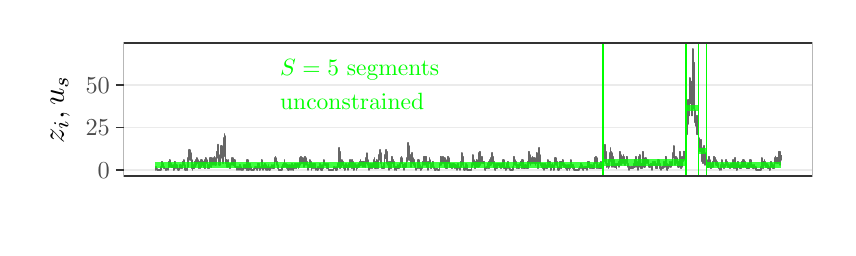
\begin{tikzpicture}[x=1pt,y=1pt]
\definecolor{fillColor}{RGB}{255,255,255}
\path[use as bounding box,fill=fillColor,fill opacity=0.00] (0,0) rectangle (289.08, 72.27);
\begin{scope}
\path[clip] (  0.00,  0.00) rectangle (289.08, 72.27);
\definecolor{drawColor}{RGB}{255,255,255}
\definecolor{fillColor}{RGB}{255,255,255}

\path[draw=drawColor,line width= 0.6pt,line join=round,line cap=round,fill=fillColor] (  0.00,  0.00) rectangle (289.08, 72.27);
\end{scope}
\begin{scope}
\path[clip] ( 34.65, 18.58) rectangle (283.58, 66.77);
\definecolor{fillColor}{RGB}{255,255,255}

\path[fill=fillColor] ( 34.65, 18.58) rectangle (283.58, 66.77);
\definecolor{drawColor}{gray}{0.92}

\path[draw=drawColor,line width= 0.6pt,line join=round] ( 34.65, 20.77) --
	(283.58, 20.77);

\path[draw=drawColor,line width= 0.6pt,line join=round] ( 34.65, 36.19) --
	(283.58, 36.19);

\path[draw=drawColor,line width= 0.6pt,line join=round] ( 34.65, 51.62) --
	(283.58, 51.62);
\definecolor{drawColor}{gray}{0.40}

\path[draw=drawColor,line width= 0.6pt,line join=round] ( 45.97, 21.38) --
	( 46.15, 21.38) --
	( 46.15, 20.77) --
	( 46.17, 20.77) --
	( 46.17, 21.38) --
	( 46.17, 21.38) --
	( 46.17, 22.00) --
	( 46.60, 22.00) --
	( 46.60, 21.38) --
	( 46.63, 21.38) --
	( 46.63, 20.77) --
	( 48.22, 20.77) --
	( 48.22, 21.38) --
	( 48.26, 21.38) --
	( 48.26, 22.00) --
	( 48.49, 22.00) --
	( 48.49, 22.62) --
	( 48.56, 22.62) --
	( 48.56, 23.23) --
	( 48.62, 23.23) --
	( 48.62, 23.85) --
	( 48.67, 23.85) --
	( 48.67, 23.23) --
	( 48.71, 23.23) --
	( 48.71, 22.62) --
	( 48.83, 22.62) --
	( 48.83, 23.23) --
	( 48.94, 23.23) --
	( 48.94, 22.62) --
	( 49.00, 22.62) --
	( 49.00, 23.23) --
	( 49.01, 23.23) --
	( 49.01, 22.62) --
	( 49.08, 22.62) --
	( 49.08, 22.00) --
	( 49.28, 22.00) --
	( 49.28, 21.38) --
	( 49.31, 21.38) --
	( 49.31, 22.00) --
	( 49.45, 22.00) --
	( 49.45, 21.38) --
	( 49.75, 21.38) --
	( 49.75, 20.77) --
	( 50.20, 20.77) --
	( 50.20, 21.38) --
	( 50.65, 21.38) --
	( 50.65, 20.77) --
	( 50.68, 20.77) --
	( 50.68, 21.38) --
	( 50.86, 21.38) --
	( 50.86, 22.00) --
	( 50.96, 22.00) --
	( 50.96, 22.62) --
	( 51.04, 22.62) --
	( 51.04, 23.23) --
	( 51.06, 23.23) --
	( 51.06, 23.85) --
	( 51.14, 23.85) --
	( 51.14, 23.23) --
	( 51.19, 23.23) --
	( 51.19, 23.85) --
	( 51.29, 23.85) --
	( 51.29, 24.47) --
	( 51.31, 24.47) --
	( 51.31, 23.85) --
	( 51.32, 23.85) --
	( 51.32, 24.47) --
	( 51.41, 24.47) --
	( 51.41, 23.85) --
	( 51.47, 23.85) --
	( 51.47, 24.47) --
	( 51.49, 24.47) --
	( 51.49, 23.85) --
	( 51.51, 23.85) --
	( 51.51, 23.23) --
	( 51.52, 23.23) --
	( 51.52, 23.85) --
	( 51.65, 23.85) --
	( 51.65, 23.23) --
	( 51.75, 23.23) --
	( 51.75, 22.62) --
	( 51.77, 22.62) --
	( 51.77, 22.00) --
	( 51.80, 22.00) --
	( 51.80, 22.62) --
	( 51.81, 22.62) --
	( 51.81, 23.23) --
	( 51.92, 23.23) --
	( 51.92, 22.62) --
	( 51.97, 22.62) --
	( 51.97, 22.00) --
	( 52.25, 22.00) --
	( 52.25, 22.62) --
	( 52.27, 22.62) --
	( 52.27, 22.00) --
	( 52.70, 22.00) --
	( 52.70, 20.77) --
	( 52.81, 20.77) --
	( 52.81, 21.38) --
	( 52.83, 21.38) --
	( 52.83, 22.00) --
	( 52.88, 22.00) --
	( 52.88, 22.62) --
	( 53.02, 22.62) --
	( 53.02, 23.23) --
	( 53.10, 23.23) --
	( 53.10, 23.85) --
	( 53.26, 23.85) --
	( 53.26, 23.23) --
	( 53.29, 23.23) --
	( 53.29, 22.62) --
	( 53.33, 22.62) --
	( 53.33, 22.00) --
	( 53.34, 22.00) --
	( 53.34, 22.62) --
	( 53.47, 22.62) --
	( 53.47, 22.00) --
	( 53.55, 22.00) --
	( 53.55, 21.38) --
	( 53.59, 21.38) --
	( 53.59, 22.00) --
	( 53.69, 22.00) --
	( 53.69, 22.62) --
	( 53.79, 22.62) --
	( 53.79, 22.00) --
	( 53.98, 22.00) --
	( 53.98, 22.62) --
	( 54.05, 22.62) --
	( 54.05, 22.00) --
	( 54.14, 22.00) --
	( 54.14, 21.38) --
	( 54.43, 21.38) --
	( 54.43, 20.77) --
	( 54.79, 20.77) --
	( 54.79, 21.38) --
	( 55.02, 21.38) --
	( 55.02, 22.00) --
	( 55.09, 22.00) --
	( 55.09, 22.62) --
	( 55.24, 22.62) --
	( 55.24, 22.00) --
	( 55.35, 22.00) --
	( 55.35, 22.62) --
	( 55.48, 22.62) --
	( 55.48, 22.00) --
	( 55.54, 22.00) --
	( 55.54, 21.38) --
	( 55.78, 21.38) --
	( 55.78, 22.00) --
	( 55.80, 22.00) --
	( 55.80, 21.38) --
	( 55.81, 21.38) --
	( 55.81, 22.00) --
	( 55.98, 22.00) --
	( 55.98, 23.23) --
	( 56.17, 23.23) --
	( 56.17, 23.85) --
	( 56.23, 23.85) --
	( 56.23, 23.23) --
	( 56.26, 23.23) --
	( 56.26, 22.62) --
	( 56.41, 22.62) --
	( 56.41, 23.85) --
	( 56.43, 23.85) --
	( 56.43, 24.47) --
	( 56.44, 24.47) --
	( 56.44, 23.23) --
	( 56.62, 23.23) --
	( 56.62, 22.62) --
	( 56.87, 22.62) --
	( 56.87, 21.38) --
	( 56.87, 21.38) --
	( 56.87, 20.77) --
	( 57.13, 20.77) --
	( 57.13, 21.38) --
	( 57.58, 21.38) --
	( 57.58, 20.77) --
	( 57.72, 20.77) --
	( 57.72, 21.38) --
	( 57.77, 21.38) --
	( 57.77, 22.00) --
	( 57.82, 22.00) --
	( 57.82, 23.23) --
	( 57.91, 23.23) --
	( 57.91, 24.47) --
	( 58.05, 24.47) --
	( 58.05, 25.09) --
	( 58.10, 25.09) --
	( 58.10, 25.70) --
	( 58.17, 25.70) --
	( 58.17, 25.09) --
	( 58.20, 25.09) --
	( 58.20, 26.94) --
	( 58.21, 26.94) --
	( 58.21, 27.55) --
	( 58.22, 27.55) --
	( 58.22, 26.94) --
	( 58.27, 26.94) --
	( 58.27, 28.17) --
	( 58.27, 28.17) --
	( 58.27, 26.94) --
	( 58.34, 26.94) --
	( 58.34, 27.55) --
	( 58.37, 27.55) --
	( 58.37, 26.32) --
	( 58.43, 26.32) --
	( 58.43, 26.94) --
	( 58.51, 26.94) --
	( 58.51, 26.32) --
	( 58.55, 26.32) --
	( 58.55, 25.70) --
	( 58.59, 25.70) --
	( 58.59, 27.55) --
	( 58.63, 27.55) --
	( 58.63, 28.17) --
	( 58.65, 28.17) --
	( 58.65, 27.55) --
	( 58.65, 27.55) --
	( 58.65, 26.32) --
	( 58.67, 26.32) --
	( 58.67, 25.70) --
	( 58.73, 25.70) --
	( 58.73, 24.47) --
	( 58.81, 24.47) --
	( 58.81, 25.09) --
	( 58.83, 25.09) --
	( 58.83, 25.70) --
	( 58.84, 25.70) --
	( 58.84, 26.32) --
	( 58.88, 26.32) --
	( 58.88, 25.70) --
	( 58.99, 25.70) --
	( 58.99, 26.32) --
	( 59.01, 26.32) --
	( 59.01, 26.94) --
	( 59.04, 26.94) --
	( 59.04, 25.09) --
	( 59.05, 25.09) --
	( 59.05, 25.70) --
	( 59.09, 25.70) --
	( 59.09, 25.09) --
	( 59.25, 25.09) --
	( 59.25, 24.47) --
	( 59.26, 24.47) --
	( 59.26, 23.85) --
	( 59.29, 23.85) --
	( 59.29, 22.62) --
	( 59.44, 22.62) --
	( 59.44, 21.38) --
	( 59.50, 21.38) --
	( 59.50, 20.77) --
	( 59.55, 20.77) --
	( 59.55, 21.38) --
	( 59.64, 21.38) --
	( 59.64, 22.00) --
	( 59.87, 22.00) --
	( 59.87, 22.62) --
	( 60.00, 22.62) --
	( 60.00, 22.00) --
	( 60.10, 22.00) --
	( 60.10, 21.38) --
	( 60.22, 21.38) --
	( 60.22, 22.00) --
	( 60.32, 22.00) --
	( 60.32, 21.38) --
	( 60.33, 21.38) --
	( 60.33, 22.00) --
	( 60.37, 22.00) --
	( 60.37, 22.62) --
	( 60.39, 22.62) --
	( 60.39, 23.23) --
	( 60.55, 23.23) --
	( 60.55, 23.85) --
	( 60.67, 23.85) --
	( 60.67, 23.23) --
	( 60.68, 23.23) --
	( 60.68, 23.85) --
	( 60.78, 23.85) --
	( 60.78, 23.23) --
	( 60.82, 23.23) --
	( 60.82, 22.62) --
	( 60.83, 22.62) --
	( 60.83, 23.85) --
	( 60.84, 23.85) --
	( 60.84, 23.23) --
	( 60.92, 23.23) --
	( 60.92, 23.85) --
	( 60.93, 23.85) --
	( 60.93, 24.47) --
	( 61.08, 24.47) --
	( 61.08, 25.09) --
	( 61.14, 25.09) --
	( 61.14, 24.47) --
	( 61.22, 24.47) --
	( 61.22, 25.09) --
	( 61.28, 25.09) --
	( 61.28, 23.85) --
	( 61.36, 23.85) --
	( 61.36, 24.47) --
	( 61.37, 24.47) --
	( 61.37, 23.85) --
	( 61.39, 23.85) --
	( 61.39, 23.23) --
	( 61.42, 23.23) --
	( 61.42, 24.47) --
	( 61.46, 24.47) --
	( 61.46, 23.85) --
	( 61.54, 23.85) --
	( 61.54, 23.23) --
	( 61.68, 23.23) --
	( 61.68, 22.62) --
	( 61.78, 22.62) --
	( 61.78, 23.23) --
	( 61.82, 23.23) --
	( 61.82, 22.62) --
	( 61.88, 22.62) --
	( 61.88, 21.38) --
	( 61.89, 21.38) --
	( 61.89, 22.00) --
	( 61.91, 22.00) --
	( 61.91, 22.62) --
	( 61.96, 22.62) --
	( 61.96, 23.23) --
	( 62.21, 23.23) --
	( 62.21, 23.85) --
	( 62.23, 23.85) --
	( 62.23, 23.23) --
	( 62.34, 23.23) --
	( 62.34, 22.62) --
	( 62.36, 22.62) --
	( 62.36, 22.00) --
	( 62.41, 22.00) --
	( 62.41, 21.38) --
	( 62.50, 21.38) --
	( 62.50, 22.00) --
	( 62.60, 22.00) --
	( 62.60, 22.62) --
	( 62.63, 22.62) --
	( 62.63, 23.23) --
	( 62.64, 23.23) --
	( 62.64, 23.85) --
	( 62.66, 23.85) --
	( 62.66, 23.23) --
	( 62.68, 23.23) --
	( 62.68, 23.85) --
	( 62.74, 23.85) --
	( 62.74, 24.47) --
	( 62.95, 24.47) --
	( 62.95, 23.85) --
	( 63.03, 23.85) --
	( 63.03, 24.47) --
	( 63.08, 24.47) --
	( 63.08, 23.85) --
	( 63.09, 23.85) --
	( 63.09, 23.23) --
	( 63.10, 23.23) --
	( 63.10, 23.85) --
	( 63.13, 23.85) --
	( 63.13, 23.23) --
	( 63.20, 23.23) --
	( 63.20, 22.62) --
	( 63.41, 22.62) --
	( 63.41, 23.23) --
	( 63.45, 23.23) --
	( 63.45, 23.85) --
	( 63.48, 23.85) --
	( 63.48, 23.23) --
	( 63.50, 23.23) --
	( 63.50, 22.62) --
	( 63.55, 22.62) --
	( 63.55, 22.00) --
	( 63.85, 22.00) --
	( 63.85, 22.62) --
	( 63.87, 22.62) --
	( 63.87, 22.00) --
	( 63.90, 22.00) --
	( 63.90, 21.38) --
	( 63.96, 21.38) --
	( 63.96, 22.00) --
	( 63.97, 22.00) --
	( 63.97, 22.62) --
	( 64.06, 22.62) --
	( 64.06, 23.23) --
	( 64.14, 23.23) --
	( 64.14, 23.85) --
	( 64.17, 23.85) --
	( 64.17, 24.47) --
	( 64.25, 24.47) --
	( 64.25, 25.09) --
	( 64.31, 25.09) --
	( 64.31, 24.47) --
	( 64.39, 24.47) --
	( 64.39, 25.09) --
	( 64.41, 25.09) --
	( 64.41, 24.47) --
	( 64.41, 24.47) --
	( 64.41, 23.85) --
	( 64.48, 23.85) --
	( 64.48, 23.23) --
	( 64.51, 23.23) --
	( 64.51, 23.85) --
	( 64.58, 23.85) --
	( 64.58, 24.47) --
	( 64.59, 24.47) --
	( 64.59, 23.85) --
	( 64.60, 23.85) --
	( 64.60, 24.47) --
	( 64.62, 24.47) --
	( 64.62, 23.85) --
	( 64.65, 23.85) --
	( 64.65, 24.47) --
	( 64.70, 24.47) --
	( 64.70, 23.85) --
	( 64.76, 23.85) --
	( 64.76, 24.47) --
	( 64.84, 24.47) --
	( 64.84, 23.85) --
	( 64.97, 23.85) --
	( 64.97, 23.23) --
	( 65.03, 23.23) --
	( 65.03, 22.62) --
	( 65.05, 22.62) --
	( 65.05, 22.00) --
	( 65.10, 22.00) --
	( 65.10, 21.38) --
	( 65.12, 21.38) --
	( 65.12, 22.00) --
	( 65.14, 22.00) --
	( 65.14, 21.38) --
	( 65.28, 21.38) --
	( 65.28, 22.00) --
	( 65.52, 22.00) --
	( 65.52, 22.62) --
	( 65.58, 22.62) --
	( 65.58, 22.00) --
	( 65.73, 22.00) --
	( 65.73, 21.38) --
	( 65.75, 21.38) --
	( 65.75, 22.62) --
	( 65.78, 22.62) --
	( 65.78, 23.23) --
	( 65.79, 23.23) --
	( 65.79, 23.85) --
	( 65.82, 23.85) --
	( 65.82, 24.47) --
	( 65.85, 24.47) --
	( 65.85, 25.09) --
	( 65.98, 25.09) --
	( 65.98, 24.47) --
	( 66.05, 24.47) --
	( 66.05, 25.09) --
	( 66.21, 25.09) --
	( 66.21, 23.85) --
	( 66.23, 23.85) --
	( 66.23, 23.23) --
	( 66.24, 23.23) --
	( 66.24, 22.62) --
	( 66.31, 22.62) --
	( 66.31, 22.00) --
	( 66.39, 22.00) --
	( 66.39, 22.62) --
	( 66.41, 22.62) --
	( 66.41, 23.85) --
	( 66.53, 23.85) --
	( 66.53, 24.47) --
	( 66.57, 24.47) --
	( 66.57, 25.09) --
	( 66.72, 25.09) --
	( 66.72, 24.47) --
	( 66.84, 24.47) --
	( 66.84, 23.85) --
	( 66.86, 23.85) --
	( 66.86, 22.62) --
	( 66.89, 22.62) --
	( 66.89, 23.23) --
	( 66.95, 23.23) --
	( 66.95, 22.62) --
	( 66.98, 22.62) --
	( 66.98, 23.23) --
	( 66.99, 23.23) --
	( 66.99, 22.62) --
	( 67.02, 22.62) --
	( 67.02, 23.23) --
	( 67.03, 23.23) --
	( 67.03, 22.62) --
	( 67.08, 22.62) --
	( 67.08, 23.23) --
	( 67.16, 23.23) --
	( 67.16, 23.85) --
	( 67.19, 23.85) --
	( 67.19, 24.47) --
	( 67.27, 24.47) --
	( 67.27, 25.09) --
	( 67.34, 25.09) --
	( 67.34, 24.47) --
	( 67.34, 24.47) --
	( 67.34, 25.09) --
	( 67.43, 25.09) --
	( 67.43, 24.47) --
	( 67.46, 24.47) --
	( 67.46, 25.09) --
	( 67.46, 25.09) --
	( 67.46, 25.70) --
	( 67.47, 25.70) --
	( 67.47, 25.09) --
	( 67.54, 25.09) --
	( 67.54, 24.47) --
	( 67.61, 24.47) --
	( 67.61, 23.85) --
	( 67.64, 23.85) --
	( 67.64, 23.23) --
	( 67.72, 23.23) --
	( 67.72, 22.62) --
	( 67.73, 22.62) --
	( 67.73, 23.23) --
	( 67.76, 23.23) --
	( 67.76, 24.47) --
	( 67.80, 24.47) --
	( 67.80, 23.85) --
	( 67.91, 23.85) --
	( 67.91, 23.23) --
	( 67.92, 23.23) --
	( 67.92, 22.62) --
	( 67.94, 22.62) --
	( 67.94, 23.23) --
	( 67.99, 23.23) --
	( 67.99, 23.85) --
	( 68.06, 23.85) --
	( 68.06, 24.47) --
	( 68.16, 24.47) --
	( 68.16, 25.09) --
	( 68.18, 25.09) --
	( 68.18, 24.47) --
	( 68.19, 24.47) --
	( 68.19, 25.09) --
	( 68.20, 25.09) --
	( 68.20, 25.70) --
	( 68.21, 25.70) --
	( 68.21, 25.09) --
	( 68.21, 25.09) --
	( 68.21, 24.47) --
	( 68.24, 24.47) --
	( 68.24, 25.09) --
	( 68.38, 25.09) --
	( 68.38, 25.70) --
	( 68.39, 25.70) --
	( 68.39, 25.09) --
	( 68.43, 25.09) --
	( 68.43, 25.70) --
	( 68.44, 25.70) --
	( 68.44, 25.09) --
	( 68.46, 25.09) --
	( 68.46, 26.94) --
	( 68.47, 26.94) --
	( 68.47, 27.55) --
	( 68.49, 27.55) --
	( 68.49, 26.94) --
	( 68.51, 26.94) --
	( 68.51, 27.55) --
	( 68.56, 27.55) --
	( 68.56, 28.17) --
	( 68.60, 28.17) --
	( 68.60, 28.79) --
	( 68.61, 28.79) --
	( 68.61, 28.17) --
	( 68.65, 28.17) --
	( 68.65, 27.55) --
	( 68.66, 27.55) --
	( 68.66, 26.94) --
	( 68.66, 26.94) --
	( 68.66, 27.55) --
	( 68.69, 27.55) --
	( 68.69, 28.17) --
	( 68.69, 28.17) --
	( 68.69, 27.55) --
	( 68.70, 27.55) --
	( 68.70, 28.79) --
	( 68.76, 28.79) --
	( 68.76, 29.41) --
	( 68.83, 29.41) --
	( 68.83, 30.02) --
	( 68.83, 30.02) --
	( 68.83, 29.41) --
	( 68.89, 29.41) --
	( 68.89, 28.79) --
	( 68.91, 28.79) --
	( 68.91, 26.94) --
	( 68.92, 26.94) --
	( 68.92, 25.70) --
	( 68.93, 25.70) --
	( 68.93, 26.32) --
	( 68.99, 26.32) --
	( 68.99, 26.94) --
	( 69.01, 26.94) --
	( 69.01, 26.32) --
	( 69.05, 26.32) --
	( 69.05, 25.70) --
	( 69.06, 25.70) --
	( 69.06, 25.09) --
	( 69.14, 25.09) --
	( 69.14, 24.47) --
	( 69.15, 24.47) --
	( 69.15, 23.23) --
	( 69.19, 23.23) --
	( 69.19, 23.85) --
	( 69.21, 23.85) --
	( 69.21, 22.62) --
	( 69.30, 22.62) --
	( 69.30, 23.23) --
	( 69.38, 23.23) --
	( 69.38, 23.85) --
	( 69.38, 23.85) --
	( 69.38, 23.23) --
	( 69.44, 23.23) --
	( 69.44, 22.62) --
	( 69.51, 22.62) --
	( 69.51, 23.85) --
	( 69.55, 23.85) --
	( 69.55, 24.47) --
	( 69.59, 24.47) --
	( 69.59, 25.09) --
	( 69.59, 25.09) --
	( 69.59, 24.47) --
	( 69.66, 24.47) --
	( 69.66, 25.09) --
	( 69.68, 25.09) --
	( 69.68, 25.70) --
	( 69.75, 25.70) --
	( 69.75, 25.09) --
	( 69.78, 25.09) --
	( 69.78, 25.70) --
	( 69.79, 25.70) --
	( 69.79, 26.32) --
	( 69.82, 26.32) --
	( 69.82, 26.94) --
	( 69.85, 26.94) --
	( 69.85, 26.32) --
	( 69.86, 26.32) --
	( 69.86, 26.94) --
	( 69.90, 26.94) --
	( 69.90, 27.55) --
	( 69.92, 27.55) --
	( 69.92, 28.17) --
	( 69.92, 28.17) --
	( 69.92, 28.79) --
	( 69.97, 28.79) --
	( 69.97, 29.41) --
	( 69.99, 29.41) --
	( 69.99, 28.79) --
	( 70.02, 28.79) --
	( 70.02, 29.41) --
	( 70.04, 29.41) --
	( 70.04, 28.79) --
	( 70.04, 28.79) --
	( 70.04, 28.17) --
	( 70.08, 28.17) --
	( 70.08, 28.79) --
	( 70.09, 28.79) --
	( 70.09, 29.41) --
	( 70.11, 29.41) --
	( 70.11, 28.79) --
	( 70.18, 28.79) --
	( 70.18, 29.41) --
	( 70.24, 29.41) --
	( 70.24, 28.79) --
	( 70.27, 28.79) --
	( 70.27, 28.17) --
	( 70.28, 28.17) --
	( 70.28, 28.79) --
	( 70.28, 28.79) --
	( 70.28, 28.17) --
	( 70.32, 28.17) --
	( 70.32, 28.79) --
	( 70.35, 28.79) --
	( 70.35, 28.17) --
	( 70.37, 28.17) --
	( 70.37, 27.55) --
	( 70.37, 27.55) --
	( 70.37, 26.94) --
	( 70.41, 26.94) --
	( 70.41, 26.32) --
	( 70.42, 26.32) --
	( 70.42, 25.70) --
	( 70.47, 25.70) --
	( 70.47, 25.09) --
	( 70.52, 25.09) --
	( 70.52, 24.47) --
	( 70.52, 24.47) --
	( 70.52, 25.09) --
	( 70.53, 25.09) --
	( 70.53, 24.47) --
	( 70.54, 24.47) --
	( 70.54, 23.85) --
	( 70.59, 23.85) --
	( 70.59, 23.23) --
	( 70.60, 23.23) --
	( 70.60, 23.85) --
	( 70.63, 23.85) --
	( 70.63, 24.47) --
	( 70.64, 24.47) --
	( 70.64, 23.85) --
	( 70.71, 23.85) --
	( 70.71, 24.47) --
	( 70.73, 24.47) --
	( 70.73, 23.85) --
	( 70.77, 23.85) --
	( 70.77, 23.23) --
	( 70.79, 23.23) --
	( 70.79, 23.85) --
	( 70.79, 23.85) --
	( 70.79, 25.09) --
	( 70.80, 25.09) --
	( 70.80, 25.70) --
	( 70.86, 25.70) --
	( 70.86, 26.32) --
	( 70.89, 26.32) --
	( 70.89, 26.94) --
	( 70.90, 26.94) --
	( 70.90, 27.55) --
	( 70.91, 27.55) --
	( 70.91, 28.17) --
	( 70.95, 28.17) --
	( 70.95, 28.79) --
	( 70.96, 28.79) --
	( 70.96, 29.41) --
	( 70.98, 29.41) --
	( 70.98, 28.79) --
	( 70.98, 28.79) --
	( 70.98, 29.41) --
	( 71.00, 29.41) --
	( 71.00, 31.26) --
	( 71.01, 31.26) --
	( 71.01, 31.87) --
	( 71.04, 31.87) --
	( 71.04, 31.26) --
	( 71.05, 31.26) --
	( 71.05, 31.87) --
	( 71.05, 31.87) --
	( 71.05, 32.49) --
	( 71.07, 32.49) --
	( 71.07, 33.11) --
	( 71.08, 33.11) --
	( 71.08, 33.73) --
	( 71.09, 33.73) --
	( 71.09, 33.11) --
	( 71.14, 33.11) --
	( 71.14, 33.73) --
	( 71.17, 33.73) --
	( 71.17, 33.11) --
	( 71.24, 33.11) --
	( 71.24, 32.49) --
	( 71.24, 32.49) --
	( 71.24, 31.87) --
	( 71.25, 31.87) --
	( 71.25, 31.26) --
	( 71.31, 31.26) --
	( 71.31, 30.64) --
	( 71.34, 30.64) --
	( 71.34, 30.02) --
	( 71.36, 30.02) --
	( 71.36, 29.41) --
	( 71.36, 29.41) --
	( 71.36, 28.79) --
	( 71.40, 28.79) --
	( 71.40, 28.17) --
	( 71.42, 28.17) --
	( 71.42, 27.55) --
	( 71.43, 27.55) --
	( 71.43, 26.94) --
	( 71.45, 26.94) --
	( 71.45, 25.09) --
	( 71.46, 25.09) --
	( 71.46, 25.70) --
	( 71.47, 25.70) --
	( 71.47, 24.47) --
	( 71.50, 24.47) --
	( 71.50, 23.85) --
	( 71.51, 23.85) --
	( 71.51, 23.23) --
	( 71.52, 23.23) --
	( 71.52, 23.85) --
	( 71.52, 23.85) --
	( 71.52, 24.47) --
	( 71.54, 24.47) --
	( 71.54, 23.85) --
	( 71.59, 23.85) --
	( 71.59, 23.23) --
	( 71.71, 23.23) --
	( 71.71, 24.47) --
	( 71.91, 24.47) --
	( 71.91, 23.85) --
	( 71.97, 23.85) --
	( 71.97, 22.00) --
	( 72.14, 22.00) --
	( 72.14, 23.23) --
	( 72.16, 23.23) --
	( 72.16, 22.00) --
	( 72.24, 22.00) --
	( 72.24, 22.62) --
	( 72.38, 22.62) --
	( 72.38, 23.23) --
	( 72.52, 23.23) --
	( 72.52, 23.85) --
	( 72.52, 23.85) --
	( 72.52, 24.47) --
	( 72.59, 24.47) --
	( 72.59, 23.23) --
	( 72.69, 23.23) --
	( 72.69, 22.62) --
	( 72.83, 22.62) --
	( 72.83, 22.00) --
	( 72.84, 22.00) --
	( 72.84, 22.62) --
	( 72.97, 22.62) --
	( 72.97, 22.00) --
	( 72.98, 22.00) --
	( 72.98, 21.38) --
	( 73.00, 21.38) --
	( 73.00, 22.00) --
	( 73.00, 22.00) --
	( 73.00, 22.62) --
	( 73.28, 22.62) --
	( 73.28, 23.23) --
	( 73.29, 23.23) --
	( 73.29, 22.62) --
	( 73.43, 22.62) --
	( 73.43, 23.23) --
	( 73.46, 23.23) --
	( 73.46, 22.62) --
	( 73.53, 22.62) --
	( 73.53, 23.23) --
	( 73.66, 23.23) --
	( 73.66, 23.85) --
	( 73.73, 23.85) --
	( 73.73, 23.23) --
	( 73.77, 23.23) --
	( 73.77, 23.85) --
	( 73.83, 23.85) --
	( 73.83, 25.09) --
	( 73.88, 25.09) --
	( 73.88, 24.47) --
	( 73.91, 24.47) --
	( 73.91, 23.85) --
	( 73.98, 23.85) --
	( 73.98, 23.23) --
	( 74.03, 23.23) --
	( 74.03, 23.85) --
	( 74.05, 23.85) --
	( 74.05, 24.47) --
	( 74.11, 24.47) --
	( 74.11, 23.85) --
	( 74.16, 23.85) --
	( 74.16, 24.47) --
	( 74.20, 24.47) --
	( 74.20, 25.09) --
	( 74.21, 25.09) --
	( 74.21, 24.47) --
	( 74.21, 24.47) --
	( 74.21, 23.85) --
	( 74.24, 23.85) --
	( 74.24, 23.23) --
	( 74.28, 23.23) --
	( 74.28, 22.62) --
	( 74.35, 22.62) --
	( 74.35, 23.23) --
	( 74.38, 23.23) --
	( 74.38, 23.85) --
	( 74.41, 23.85) --
	( 74.41, 23.23) --
	( 74.49, 23.23) --
	( 74.49, 22.62) --
	( 74.52, 22.62) --
	( 74.52, 23.23) --
	( 74.52, 23.23) --
	( 74.52, 23.85) --
	( 74.62, 23.85) --
	( 74.62, 24.47) --
	( 74.65, 24.47) --
	( 74.65, 23.85) --
	( 74.65, 23.85) --
	( 74.65, 24.47) --
	( 74.81, 24.47) --
	( 74.81, 23.85) --
	( 74.83, 23.85) --
	( 74.83, 23.23) --
	( 74.96, 23.23) --
	( 74.96, 22.00) --
	( 75.05, 22.00) --
	( 75.05, 22.62) --
	( 75.07, 22.62) --
	( 75.07, 22.00) --
	( 75.08, 22.00) --
	( 75.08, 22.62) --
	( 75.10, 22.62) --
	( 75.10, 22.00) --
	( 75.50, 22.00) --
	( 75.50, 21.38) --
	( 75.53, 21.38) --
	( 75.53, 20.77) --
	( 75.72, 20.77) --
	( 75.72, 21.38) --
	( 75.83, 21.38) --
	( 75.83, 22.00) --
	( 76.12, 22.00) --
	( 76.12, 21.38) --
	( 76.28, 21.38) --
	( 76.28, 20.77) --
	( 76.47, 20.77) --
	( 76.47, 21.38) --
	( 76.53, 21.38) --
	( 76.53, 22.00) --
	( 76.54, 22.00) --
	( 76.54, 22.62) --
	( 76.91, 22.62) --
	( 76.91, 22.00) --
	( 76.98, 22.00) --
	( 76.98, 21.38) --
	( 76.99, 21.38) --
	( 76.99, 20.77) --
	( 77.22, 20.77) --
	( 77.22, 21.38) --
	( 77.68, 21.38) --
	( 77.68, 20.77) --
	( 77.89, 20.77) --
	( 77.89, 21.38) --
	( 78.02, 21.38) --
	( 78.02, 22.00) --
	( 78.20, 22.00) --
	( 78.20, 22.62) --
	( 78.24, 22.62) --
	( 78.24, 22.00) --
	( 78.35, 22.00) --
	( 78.35, 21.38) --
	( 78.51, 21.38) --
	( 78.51, 22.00) --
	( 78.57, 22.00) --
	( 78.57, 22.62) --
	( 78.65, 22.62) --
	( 78.65, 22.00) --
	( 78.96, 22.00) --
	( 78.96, 21.38) --
	( 79.02, 21.38) --
	( 79.02, 20.77) --
	( 79.20, 20.77) --
	( 79.20, 22.62) --
	( 79.23, 22.62) --
	( 79.23, 24.47) --
	( 79.65, 24.47) --
	( 79.65, 22.62) --
	( 79.68, 22.62) --
	( 79.68, 22.00) --
	( 79.68, 22.00) --
	( 79.68, 20.77) --
	( 79.92, 20.77) --
	( 79.92, 21.38) --
	( 79.96, 21.38) --
	( 79.96, 22.00) --
	( 80.14, 22.00) --
	( 80.14, 22.62) --
	( 80.29, 22.62) --
	( 80.29, 23.23) --
	( 80.35, 23.23) --
	( 80.35, 22.62) --
	( 80.41, 22.62) --
	( 80.41, 22.00) --
	( 80.59, 22.00) --
	( 80.59, 21.38) --
	( 80.73, 21.38) --
	( 80.73, 20.77) --
	( 81.78, 20.77) --
	( 81.78, 21.38) --
	( 82.03, 21.38) --
	( 82.03, 22.00) --
	( 82.24, 22.00) --
	( 82.24, 21.38) --
	( 82.27, 21.38) --
	( 82.27, 22.00) --
	( 82.48, 22.00) --
	( 82.48, 21.38) --
	( 82.53, 21.38) --
	( 82.53, 22.00) --
	( 82.72, 22.00) --
	( 82.72, 21.38) --
	( 82.98, 21.38) --
	( 82.98, 20.77) --
	( 83.02, 20.77) --
	( 83.02, 21.38) --
	( 83.25, 21.38) --
	( 83.25, 22.00) --
	( 83.27, 22.00) --
	( 83.27, 22.62) --
	( 83.29, 22.62) --
	( 83.29, 23.23) --
	( 83.47, 23.23) --
	( 83.47, 22.62) --
	( 83.70, 22.62) --
	( 83.70, 22.00) --
	( 83.73, 22.00) --
	( 83.73, 21.38) --
	( 83.74, 21.38) --
	( 83.74, 20.77) --
	( 83.84, 20.77) --
	( 83.84, 21.38) --
	( 84.23, 21.38) --
	( 84.23, 22.00) --
	( 84.30, 22.00) --
	( 84.30, 21.38) --
	( 84.38, 21.38) --
	( 84.38, 22.00) --
	( 84.46, 22.00) --
	( 84.46, 22.62) --
	( 84.49, 22.62) --
	( 84.49, 23.85) --
	( 84.50, 23.85) --
	( 84.50, 24.47) --
	( 84.68, 24.47) --
	( 84.68, 23.85) --
	( 84.83, 23.85) --
	( 84.83, 23.23) --
	( 84.91, 23.23) --
	( 84.91, 22.62) --
	( 84.94, 22.62) --
	( 84.94, 21.38) --
	( 84.96, 21.38) --
	( 84.96, 20.77) --
	( 84.99, 20.77) --
	( 84.99, 21.38) --
	( 85.22, 21.38) --
	( 85.22, 22.00) --
	( 85.44, 22.00) --
	( 85.44, 21.38) --
	( 85.57, 21.38) --
	( 85.57, 22.00) --
	( 85.63, 22.00) --
	( 85.63, 23.23) --
	( 85.67, 23.23) --
	( 85.67, 22.62) --
	( 86.02, 22.62) --
	( 86.02, 22.00) --
	( 86.08, 22.00) --
	( 86.08, 20.77) --
	( 86.14, 20.77) --
	( 86.14, 21.38) --
	( 86.38, 21.38) --
	( 86.38, 22.00) --
	( 86.59, 22.00) --
	( 86.59, 20.77) --
	( 86.65, 20.77) --
	( 86.65, 21.38) --
	( 86.80, 21.38) --
	( 86.80, 22.00) --
	( 87.05, 22.00) --
	( 87.05, 22.62) --
	( 87.08, 22.62) --
	( 87.08, 22.00) --
	( 87.24, 22.00) --
	( 87.24, 20.77) --
	( 87.50, 20.77) --
	( 87.50, 21.38) --
	( 87.93, 21.38) --
	( 87.93, 22.00) --
	( 87.95, 22.00) --
	( 87.95, 21.38) --
	( 88.03, 21.38) --
	( 88.03, 22.00) --
	( 88.20, 22.00) --
	( 88.20, 22.62) --
	( 88.38, 22.62) --
	( 88.38, 22.00) --
	( 88.48, 22.00) --
	( 88.48, 21.38) --
	( 88.50, 21.38) --
	( 88.50, 22.00) --
	( 88.63, 22.00) --
	( 88.63, 21.38) --
	( 88.76, 21.38) --
	( 88.76, 22.00) --
	( 88.95, 22.00) --
	( 88.95, 21.38) --
	( 89.10, 21.38) --
	( 89.10, 22.00) --
	( 89.12, 22.00) --
	( 89.12, 22.62) --
	( 89.17, 22.62) --
	( 89.17, 23.85) --
	( 89.21, 23.85) --
	( 89.21, 23.23) --
	( 89.25, 23.23) --
	( 89.25, 23.85) --
	( 89.28, 23.85) --
	( 89.28, 24.47) --
	( 89.39, 24.47) --
	( 89.39, 25.09) --
	( 89.50, 25.09) --
	( 89.50, 25.70) --
	( 89.56, 25.70) --
	( 89.56, 25.09) --
	( 89.56, 25.09) --
	( 89.56, 25.70) --
	( 89.57, 25.70) --
	( 89.57, 25.09) --
	( 89.62, 25.09) --
	( 89.62, 23.85) --
	( 89.69, 23.85) --
	( 89.69, 24.47) --
	( 89.70, 24.47) --
	( 89.70, 23.85) --
	( 89.71, 23.85) --
	( 89.71, 24.47) --
	( 89.73, 24.47) --
	( 89.73, 23.85) --
	( 89.81, 23.85) --
	( 89.81, 24.47) --
	( 89.84, 24.47) --
	( 89.84, 23.85) --
	( 89.95, 23.85) --
	( 89.95, 23.23) --
	( 89.99, 23.23) --
	( 89.99, 23.85) --
	( 90.02, 23.85) --
	( 90.02, 23.23) --
	( 90.08, 23.23) --
	( 90.08, 23.85) --
	( 90.14, 23.85) --
	( 90.14, 23.23) --
	( 90.15, 23.23) --
	( 90.15, 22.62) --
	( 90.22, 22.62) --
	( 90.22, 23.23) --
	( 90.26, 23.23) --
	( 90.26, 22.62) --
	( 90.44, 22.62) --
	( 90.44, 22.00) --
	( 90.53, 22.00) --
	( 90.53, 21.38) --
	( 90.67, 21.38) --
	( 90.67, 20.77) --
	( 91.90, 20.77) --
	( 91.90, 21.38) --
	( 91.93, 21.38) --
	( 91.93, 22.00) --
	( 92.07, 22.00) --
	( 92.07, 22.62) --
	( 92.35, 22.62) --
	( 92.35, 22.00) --
	( 92.36, 22.00) --
	( 92.36, 22.62) --
	( 92.38, 22.62) --
	( 92.38, 23.23) --
	( 92.38, 23.23) --
	( 92.38, 22.62) --
	( 92.52, 22.62) --
	( 92.52, 22.00) --
	( 92.61, 22.00) --
	( 92.61, 22.62) --
	( 92.68, 22.62) --
	( 92.68, 23.23) --
	( 92.79, 23.23) --
	( 92.79, 24.47) --
	( 92.81, 24.47) --
	( 92.81, 23.85) --
	( 92.83, 23.85) --
	( 92.83, 23.23) --
	( 93.06, 23.23) --
	( 93.06, 22.62) --
	( 93.10, 22.62) --
	( 93.10, 23.23) --
	( 93.14, 23.23) --
	( 93.14, 22.62) --
	( 93.16, 22.62) --
	( 93.16, 23.23) --
	( 93.24, 23.23) --
	( 93.24, 22.00) --
	( 93.52, 22.00) --
	( 93.52, 22.62) --
	( 93.56, 22.62) --
	( 93.56, 22.00) --
	( 93.61, 22.00) --
	( 93.61, 21.38) --
	( 93.64, 21.38) --
	( 93.64, 22.00) --
	( 93.72, 22.00) --
	( 93.72, 22.62) --
	( 93.97, 22.62) --
	( 93.97, 22.00) --
	( 94.09, 22.00) --
	( 94.09, 21.38) --
	( 94.17, 21.38) --
	( 94.17, 20.77) --
	( 94.42, 20.77) --
	( 94.42, 21.38) --
	( 94.42, 21.38) --
	( 94.42, 22.00) --
	( 94.75, 22.00) --
	( 94.75, 22.62) --
	( 94.87, 22.62) --
	( 94.87, 21.38) --
	( 95.20, 21.38) --
	( 95.20, 20.77) --
	( 95.21, 20.77) --
	( 95.21, 21.38) --
	( 95.39, 21.38) --
	( 95.39, 22.00) --
	( 95.47, 22.00) --
	( 95.47, 22.62) --
	( 95.49, 22.62) --
	( 95.49, 23.23) --
	( 95.67, 23.23) --
	( 95.67, 22.62) --
	( 95.84, 22.62) --
	( 95.84, 22.00) --
	( 95.92, 22.00) --
	( 95.92, 21.38) --
	( 95.95, 21.38) --
	( 95.95, 20.77) --
	( 96.00, 20.77) --
	( 96.00, 21.38) --
	( 96.37, 21.38) --
	( 96.37, 22.00) --
	( 96.44, 22.00) --
	( 96.44, 22.62) --
	( 96.45, 22.62) --
	( 96.45, 22.00) --
	( 96.45, 22.00) --
	( 96.45, 22.62) --
	( 96.56, 22.62) --
	( 96.56, 23.23) --
	( 96.82, 23.23) --
	( 96.82, 22.62) --
	( 96.84, 22.62) --
	( 96.84, 23.23) --
	( 96.89, 23.23) --
	( 96.89, 22.62) --
	( 96.90, 22.62) --
	( 96.90, 22.00) --
	( 97.01, 22.00) --
	( 97.01, 21.38) --
	( 97.14, 21.38) --
	( 97.14, 22.00) --
	( 97.22, 22.00) --
	( 97.22, 22.62) --
	( 97.30, 22.62) --
	( 97.30, 22.00) --
	( 97.35, 22.00) --
	( 97.35, 22.62) --
	( 97.44, 22.62) --
	( 97.44, 23.23) --
	( 97.58, 23.23) --
	( 97.58, 22.62) --
	( 97.60, 22.62) --
	( 97.60, 23.23) --
	( 97.67, 23.23) --
	( 97.67, 22.62) --
	( 97.81, 22.62) --
	( 97.81, 22.00) --
	( 97.89, 22.00) --
	( 97.89, 21.38) --
	( 97.92, 21.38) --
	( 97.92, 22.00) --
	( 97.95, 22.00) --
	( 97.95, 22.62) --
	( 98.06, 22.62) --
	( 98.06, 22.00) --
	( 98.11, 22.00) --
	( 98.11, 22.62) --
	( 98.19, 22.62) --
	( 98.19, 22.00) --
	( 98.20, 22.00) --
	( 98.20, 22.62) --
	( 98.32, 22.62) --
	( 98.32, 23.23) --
	( 98.36, 23.23) --
	( 98.36, 23.85) --
	( 98.42, 23.85) --
	( 98.42, 24.47) --
	( 98.50, 24.47) --
	( 98.50, 25.09) --
	( 98.56, 25.09) --
	( 98.56, 24.47) --
	( 98.65, 24.47) --
	( 98.65, 23.85) --
	( 98.70, 23.85) --
	( 98.70, 24.47) --
	( 98.70, 24.47) --
	( 98.70, 25.09) --
	( 98.76, 25.09) --
	( 98.76, 25.70) --
	( 98.77, 25.70) --
	( 98.77, 25.09) --
	( 98.81, 25.09) --
	( 98.81, 24.47) --
	( 98.83, 24.47) --
	( 98.83, 25.09) --
	( 98.85, 25.09) --
	( 98.85, 23.85) --
	( 98.96, 23.85) --
	( 98.96, 23.23) --
	( 98.96, 23.23) --
	( 98.96, 23.85) --
	( 99.12, 23.85) --
	( 99.12, 24.47) --
	( 99.15, 24.47) --
	( 99.15, 23.85) --
	( 99.16, 23.85) --
	( 99.16, 23.23) --
	( 99.16, 23.23) --
	( 99.16, 23.85) --
	( 99.19, 23.85) --
	( 99.19, 24.47) --
	( 99.21, 24.47) --
	( 99.21, 25.09) --
	( 99.21, 25.09) --
	( 99.21, 24.47) --
	( 99.25, 24.47) --
	( 99.25, 25.09) --
	( 99.29, 25.09) --
	( 99.29, 24.47) --
	( 99.39, 24.47) --
	( 99.39, 25.09) --
	( 99.41, 25.09) --
	( 99.41, 24.47) --
	( 99.49, 24.47) --
	( 99.49, 25.09) --
	( 99.57, 25.09) --
	( 99.57, 24.47) --
	( 99.61, 24.47) --
	( 99.61, 23.85) --
	( 99.64, 23.85) --
	( 99.64, 23.23) --
	( 99.65, 23.23) --
	( 99.65, 23.85) --
	( 99.70, 23.85) --
	( 99.70, 23.23) --
	( 99.84, 23.23) --
	( 99.84, 22.62) --
	( 99.86, 22.62) --
	( 99.86, 22.00) --
	( 99.88, 22.00) --
	( 99.88, 22.62) --
	( 99.89, 22.62) --
	( 99.89, 23.23) --
	(100.10, 23.23) --
	(100.10, 22.62) --
	(100.18, 22.62) --
	(100.18, 23.23) --
	(100.24, 23.23) --
	(100.24, 23.85) --
	(100.26, 23.85) --
	(100.26, 24.47) --
	(100.32, 24.47) --
	(100.32, 25.70) --
	(100.34, 25.70) --
	(100.34, 25.09) --
	(100.34, 25.09) --
	(100.34, 24.47) --
	(100.38, 24.47) --
	(100.38, 25.09) --
	(100.40, 25.09) --
	(100.40, 24.47) --
	(100.49, 24.47) --
	(100.49, 25.09) --
	(100.63, 25.09) --
	(100.63, 24.47) --
	(100.68, 24.47) --
	(100.68, 23.85) --
	(100.71, 23.85) --
	(100.71, 23.23) --
	(100.73, 23.23) --
	(100.73, 24.47) --
	(100.77, 24.47) --
	(100.77, 23.85) --
	(100.77, 23.85) --
	(100.77, 23.23) --
	(100.78, 23.23) --
	(100.78, 23.85) --
	(100.83, 23.85) --
	(100.83, 23.23) --
	(100.94, 23.23) --
	(100.94, 22.62) --
	(101.19, 22.62) --
	(101.19, 21.38) --
	(101.22, 21.38) --
	(101.22, 20.77) --
	(101.29, 20.77) --
	(101.29, 21.38) --
	(101.52, 21.38) --
	(101.52, 22.00) --
	(101.68, 22.00) --
	(101.68, 22.62) --
	(101.74, 22.62) --
	(101.74, 22.00) --
	(101.93, 22.00) --
	(101.93, 23.23) --
	(101.97, 23.23) --
	(101.97, 22.62) --
	(101.98, 22.62) --
	(101.98, 23.85) --
	(102.05, 23.85) --
	(102.05, 24.47) --
	(102.13, 24.47) --
	(102.13, 23.85) --
	(102.16, 23.85) --
	(102.16, 23.23) --
	(102.19, 23.23) --
	(102.19, 23.85) --
	(102.38, 23.85) --
	(102.38, 23.23) --
	(102.43, 23.23) --
	(102.43, 22.62) --
	(102.43, 22.62) --
	(102.43, 22.00) --
	(102.50, 22.00) --
	(102.50, 20.77) --
	(102.51, 20.77) --
	(102.51, 21.38) --
	(102.68, 21.38) --
	(102.68, 22.00) --
	(102.81, 22.00) --
	(102.81, 22.62) --
	(102.85, 22.62) --
	(102.85, 23.23) --
	(102.96, 23.23) --
	(102.96, 22.62) --
	(103.13, 22.62) --
	(103.13, 22.00) --
	(103.26, 22.00) --
	(103.26, 21.38) --
	(103.29, 21.38) --
	(103.29, 22.00) --
	(103.33, 22.00) --
	(103.33, 22.62) --
	(103.55, 22.62) --
	(103.55, 23.23) --
	(103.74, 23.23) --
	(103.74, 22.62) --
	(103.75, 22.62) --
	(103.75, 22.00) --
	(103.78, 22.00) --
	(103.78, 21.38) --
	(104.00, 21.38) --
	(104.00, 20.77) --
	(104.01, 20.77) --
	(104.01, 21.38) --
	(104.46, 21.38) --
	(104.46, 20.77) --
	(104.81, 20.77) --
	(104.81, 21.38) --
	(105.00, 21.38) --
	(105.00, 22.00) --
	(105.13, 22.00) --
	(105.13, 21.38) --
	(105.41, 21.38) --
	(105.41, 22.00) --
	(105.45, 22.00) --
	(105.45, 21.38) --
	(105.46, 21.38) --
	(105.46, 22.00) --
	(105.49, 22.00) --
	(105.49, 22.62) --
	(105.63, 22.62) --
	(105.63, 23.23) --
	(105.86, 23.23) --
	(105.86, 22.62) --
	(105.91, 22.62) --
	(105.91, 22.00) --
	(105.94, 22.00) --
	(105.94, 21.38) --
	(106.08, 21.38) --
	(106.08, 20.77) --
	(106.54, 20.77) --
	(106.54, 21.38) --
	(106.70, 21.38) --
	(106.70, 22.00) --
	(106.79, 22.00) --
	(106.79, 22.62) --
	(106.85, 22.62) --
	(106.85, 23.23) --
	(106.91, 23.23) --
	(106.91, 23.85) --
	(106.99, 23.85) --
	(106.99, 23.23) --
	(107.11, 23.23) --
	(107.11, 23.85) --
	(107.13, 23.85) --
	(107.13, 24.47) --
	(107.15, 24.47) --
	(107.15, 23.85) --
	(107.24, 23.85) --
	(107.24, 23.23) --
	(107.30, 23.23) --
	(107.30, 22.62) --
	(107.35, 22.62) --
	(107.35, 23.23) --
	(107.36, 23.23) --
	(107.36, 22.62) --
	(107.48, 22.62) --
	(107.48, 23.23) --
	(107.56, 23.23) --
	(107.56, 22.62) --
	(107.70, 22.62) --
	(107.70, 23.23) --
	(107.80, 23.23) --
	(107.80, 22.62) --
	(107.80, 22.62) --
	(107.80, 23.23) --
	(107.93, 23.23) --
	(107.93, 22.62) --
	(108.03, 22.62) --
	(108.03, 22.00) --
	(108.04, 22.00) --
	(108.04, 22.62) --
	(108.15, 22.62) --
	(108.15, 22.00) --
	(108.25, 22.00) --
	(108.25, 21.38) --
	(108.28, 21.38) --
	(108.28, 22.00) --
	(108.46, 22.00) --
	(108.46, 22.62) --
	(108.47, 22.62) --
	(108.47, 23.23) --
	(108.49, 23.23) --
	(108.49, 22.62) --
	(108.56, 22.62) --
	(108.56, 22.00) --
	(108.64, 22.00) --
	(108.64, 21.38) --
	(108.75, 21.38) --
	(108.75, 20.77) --
	(110.49, 20.77) --
	(110.49, 21.38) --
	(110.76, 21.38) --
	(110.76, 22.00) --
	(110.94, 22.00) --
	(110.94, 21.38) --
	(111.20, 21.38) --
	(111.20, 20.77) --
	(111.82, 20.77) --
	(111.82, 21.38) --
	(111.87, 21.38) --
	(111.87, 22.00) --
	(112.22, 22.00) --
	(112.22, 22.62) --
	(112.24, 22.62) --
	(112.24, 23.23) --
	(112.27, 23.23) --
	(112.27, 22.62) --
	(112.31, 22.62) --
	(112.31, 24.47) --
	(112.32, 24.47) --
	(112.32, 23.85) --
	(112.33, 23.85) --
	(112.33, 25.70) --
	(112.36, 25.70) --
	(112.36, 26.32) --
	(112.40, 26.32) --
	(112.40, 26.94) --
	(112.41, 26.94) --
	(112.41, 27.55) --
	(112.48, 27.55) --
	(112.48, 28.17) --
	(112.50, 28.17) --
	(112.50, 28.79) --
	(112.67, 28.79) --
	(112.67, 28.17) --
	(112.70, 28.17) --
	(112.70, 27.55) --
	(112.76, 27.55) --
	(112.76, 26.94) --
	(112.76, 26.94) --
	(112.76, 25.70) --
	(112.79, 25.70) --
	(112.79, 23.85) --
	(112.81, 23.85) --
	(112.81, 24.47) --
	(112.81, 24.47) --
	(112.81, 23.85) --
	(112.86, 23.85) --
	(112.86, 23.23) --
	(112.86, 23.23) --
	(112.86, 22.62) --
	(112.93, 22.62) --
	(112.93, 22.00) --
	(112.95, 22.00) --
	(112.95, 21.38) --
	(113.05, 21.38) --
	(113.05, 22.00) --
	(113.20, 22.00) --
	(113.20, 22.62) --
	(113.21, 22.62) --
	(113.21, 23.23) --
	(113.25, 23.23) --
	(113.25, 22.62) --
	(113.26, 22.62) --
	(113.26, 22.00) --
	(113.34, 22.00) --
	(113.34, 22.62) --
	(113.49, 22.62) --
	(113.49, 23.23) --
	(113.55, 23.23) --
	(113.55, 23.85) --
	(113.58, 23.85) --
	(113.58, 24.47) --
	(113.64, 24.47) --
	(113.64, 23.85) --
	(113.65, 23.85) --
	(113.65, 22.62) --
	(113.66, 22.62) --
	(113.66, 23.23) --
	(113.75, 23.23) --
	(113.75, 23.85) --
	(113.79, 23.85) --
	(113.79, 23.23) --
	(113.84, 23.23) --
	(113.84, 23.85) --
	(114.00, 23.85) --
	(114.00, 23.23) --
	(114.03, 23.23) --
	(114.03, 22.62) --
	(114.05, 22.62) --
	(114.05, 23.23) --
	(114.11, 23.23) --
	(114.11, 22.62) --
	(114.20, 22.62) --
	(114.20, 22.00) --
	(114.28, 22.00) --
	(114.28, 21.38) --
	(114.50, 21.38) --
	(114.50, 20.77) --
	(114.70, 20.77) --
	(114.70, 21.38) --
	(114.75, 21.38) --
	(114.75, 22.00) --
	(114.95, 22.00) --
	(114.95, 22.62) --
	(115.13, 22.62) --
	(115.13, 23.23) --
	(115.15, 23.23) --
	(115.15, 22.62) --
	(115.20, 22.62) --
	(115.20, 22.00) --
	(115.30, 22.00) --
	(115.30, 22.62) --
	(115.40, 22.62) --
	(115.40, 22.00) --
	(115.58, 22.00) --
	(115.58, 21.38) --
	(115.76, 21.38) --
	(115.76, 20.77) --
	(115.85, 20.77) --
	(115.85, 21.38) --
	(115.89, 21.38) --
	(115.89, 22.00) --
	(115.99, 22.00) --
	(115.99, 22.62) --
	(116.02, 22.62) --
	(116.02, 23.23) --
	(116.25, 23.23) --
	(116.25, 23.85) --
	(116.30, 23.85) --
	(116.30, 23.23) --
	(116.34, 23.23) --
	(116.34, 22.62) --
	(116.42, 22.62) --
	(116.42, 23.23) --
	(116.44, 23.23) --
	(116.44, 22.62) --
	(116.47, 22.62) --
	(116.47, 22.00) --
	(116.50, 22.00) --
	(116.50, 22.62) --
	(116.53, 22.62) --
	(116.53, 23.23) --
	(116.53, 23.23) --
	(116.53, 23.85) --
	(116.55, 23.85) --
	(116.55, 24.47) --
	(116.71, 24.47) --
	(116.71, 23.85) --
	(116.77, 23.85) --
	(116.77, 23.23) --
	(116.92, 23.23) --
	(116.92, 23.85) --
	(116.96, 23.85) --
	(116.96, 23.23) --
	(116.98, 23.23) --
	(116.98, 22.62) --
	(116.98, 22.62) --
	(116.98, 22.00) --
	(117.01, 22.00) --
	(117.01, 21.38) --
	(117.04, 21.38) --
	(117.04, 22.00) --
	(117.05, 22.00) --
	(117.05, 22.62) --
	(117.10, 22.62) --
	(117.10, 23.23) --
	(117.15, 23.23) --
	(117.15, 23.85) --
	(117.26, 23.85) --
	(117.26, 24.47) --
	(117.37, 24.47) --
	(117.37, 23.85) --
	(117.44, 23.85) --
	(117.44, 23.23) --
	(117.49, 23.23) --
	(117.49, 22.62) --
	(117.55, 22.62) --
	(117.55, 22.00) --
	(117.60, 22.00) --
	(117.60, 21.38) --
	(117.71, 21.38) --
	(117.71, 20.77) --
	(117.94, 20.77) --
	(117.94, 21.38) --
	(118.14, 21.38) --
	(118.14, 22.00) --
	(118.35, 22.00) --
	(118.35, 22.62) --
	(118.35, 22.62) --
	(118.35, 23.23) --
	(118.39, 23.23) --
	(118.39, 22.62) --
	(118.59, 22.62) --
	(118.59, 22.00) --
	(118.79, 22.00) --
	(118.79, 21.38) --
	(118.80, 21.38) --
	(118.80, 20.77) --
	(118.83, 20.77) --
	(118.83, 21.38) --
	(119.05, 21.38) --
	(119.05, 22.00) --
	(119.27, 22.00) --
	(119.27, 22.62) --
	(119.29, 22.62) --
	(119.29, 22.00) --
	(119.44, 22.00) --
	(119.44, 22.62) --
	(119.50, 22.62) --
	(119.50, 22.00) --
	(119.54, 22.00) --
	(119.54, 22.62) --
	(119.72, 22.62) --
	(119.72, 22.00) --
	(119.82, 22.00) --
	(119.82, 22.62) --
	(119.83, 22.62) --
	(119.83, 23.23) --
	(119.85, 23.23) --
	(119.85, 23.85) --
	(119.89, 23.85) --
	(119.89, 23.23) --
	(120.00, 23.23) --
	(120.00, 22.62) --
	(120.23, 22.62) --
	(120.23, 23.23) --
	(120.25, 23.23) --
	(120.25, 24.47) --
	(120.27, 24.47) --
	(120.27, 23.85) --
	(120.29, 23.85) --
	(120.29, 23.23) --
	(120.30, 23.23) --
	(120.30, 22.62) --
	(120.47, 22.62) --
	(120.47, 23.23) --
	(120.48, 23.23) --
	(120.48, 22.62) --
	(120.53, 22.62) --
	(120.53, 23.23) --
	(120.66, 23.23) --
	(120.66, 23.85) --
	(120.70, 23.85) --
	(120.70, 22.62) --
	(120.87, 22.62) --
	(120.87, 23.23) --
	(120.91, 23.23) --
	(120.91, 22.62) --
	(120.95, 22.62) --
	(120.95, 23.23) --
	(120.98, 23.23) --
	(120.98, 22.62) --
	(121.11, 22.62) --
	(121.11, 22.00) --
	(121.12, 22.00) --
	(121.12, 22.62) --
	(121.20, 22.62) --
	(121.20, 23.23) --
	(121.26, 23.23) --
	(121.26, 23.85) --
	(121.32, 23.85) --
	(121.32, 23.23) --
	(121.34, 23.23) --
	(121.34, 23.85) --
	(121.40, 23.85) --
	(121.40, 23.23) --
	(121.47, 23.23) --
	(121.47, 23.85) --
	(121.56, 23.85) --
	(121.56, 23.23) --
	(121.65, 23.23) --
	(121.65, 22.62) --
	(121.67, 22.62) --
	(121.67, 23.23) --
	(121.70, 23.23) --
	(121.70, 23.85) --
	(121.71, 23.85) --
	(121.71, 23.23) --
	(121.79, 23.23) --
	(121.79, 22.62) --
	(121.91, 22.62) --
	(121.91, 22.00) --
	(122.02, 22.00) --
	(122.02, 22.62) --
	(122.10, 22.62) --
	(122.10, 23.23) --
	(122.12, 23.23) --
	(122.12, 22.62) --
	(122.13, 22.62) --
	(122.13, 23.23) --
	(122.15, 23.23) --
	(122.15, 24.47) --
	(122.16, 24.47) --
	(122.16, 23.85) --
	(122.18, 23.85) --
	(122.18, 24.47) --
	(122.30, 24.47) --
	(122.30, 25.09) --
	(122.40, 25.09) --
	(122.40, 25.70) --
	(122.44, 25.70) --
	(122.44, 26.32) --
	(122.48, 26.32) --
	(122.48, 25.70) --
	(122.49, 25.70) --
	(122.49, 26.32) --
	(122.55, 26.32) --
	(122.55, 26.94) --
	(122.55, 26.94) --
	(122.55, 26.32) --
	(122.59, 26.32) --
	(122.59, 25.70) --
	(122.60, 25.70) --
	(122.60, 26.32) --
	(122.60, 26.32) --
	(122.60, 25.70) --
	(122.61, 25.70) --
	(122.61, 25.09) --
	(122.63, 25.09) --
	(122.63, 24.47) --
	(122.65, 24.47) --
	(122.65, 25.09) --
	(122.74, 25.09) --
	(122.74, 25.70) --
	(122.75, 25.70) --
	(122.75, 25.09) --
	(122.85, 25.09) --
	(122.85, 24.47) --
	(122.89, 24.47) --
	(122.89, 23.85) --
	(122.94, 23.85) --
	(122.94, 24.47) --
	(122.94, 24.47) --
	(122.94, 23.85) --
	(123.00, 23.85) --
	(123.00, 23.23) --
	(123.05, 23.23) --
	(123.05, 22.62) --
	(123.10, 22.62) --
	(123.10, 22.00) --
	(123.20, 22.00) --
	(123.20, 21.38) --
	(123.39, 21.38) --
	(123.39, 20.77) --
	(123.42, 20.77) --
	(123.42, 21.38) --
	(123.61, 21.38) --
	(123.61, 22.00) --
	(123.68, 22.00) --
	(123.68, 22.62) --
	(123.73, 22.62) --
	(123.73, 23.23) --
	(123.84, 23.23) --
	(123.84, 22.62) --
	(123.94, 22.62) --
	(123.94, 23.23) --
	(124.06, 23.23) --
	(124.06, 22.62) --
	(124.07, 22.62) --
	(124.07, 23.23) --
	(124.12, 23.23) --
	(124.12, 22.62) --
	(124.18, 22.62) --
	(124.18, 22.00) --
	(124.39, 22.00) --
	(124.39, 21.38) --
	(124.40, 21.38) --
	(124.40, 22.00) --
	(124.46, 22.00) --
	(124.46, 22.62) --
	(124.52, 22.62) --
	(124.52, 22.00) --
	(124.54, 22.00) --
	(124.54, 22.62) --
	(124.84, 22.62) --
	(124.84, 23.23) --
	(124.85, 23.23) --
	(124.85, 22.62) --
	(124.91, 22.62) --
	(124.91, 22.00) --
	(124.91, 22.00) --
	(124.91, 22.62) --
	(124.98, 22.62) --
	(124.98, 22.00) --
	(125.00, 22.00) --
	(125.00, 22.62) --
	(125.04, 22.62) --
	(125.04, 23.23) --
	(125.07, 23.23) --
	(125.07, 23.85) --
	(125.23, 23.85) --
	(125.23, 24.47) --
	(125.27, 24.47) --
	(125.27, 25.09) --
	(125.29, 25.09) --
	(125.29, 24.47) --
	(125.36, 24.47) --
	(125.36, 23.85) --
	(125.38, 23.85) --
	(125.38, 23.23) --
	(125.45, 23.23) --
	(125.45, 22.62) --
	(125.49, 22.62) --
	(125.49, 22.00) --
	(125.52, 22.00) --
	(125.52, 21.38) --
	(125.59, 21.38) --
	(125.59, 22.00) --
	(125.68, 22.00) --
	(125.68, 22.62) --
	(125.72, 22.62) --
	(125.72, 22.00) --
	(125.84, 22.00) --
	(125.84, 21.38) --
	(125.84, 21.38) --
	(125.84, 22.00) --
	(125.91, 22.00) --
	(125.91, 22.62) --
	(125.92, 22.62) --
	(125.92, 23.23) --
	(125.98, 23.23) --
	(125.98, 23.85) --
	(126.01, 23.85) --
	(126.01, 24.47) --
	(126.13, 24.47) --
	(126.13, 23.85) --
	(126.28, 23.85) --
	(126.28, 24.47) --
	(126.30, 24.47) --
	(126.30, 23.85) --
	(126.37, 23.85) --
	(126.37, 23.23) --
	(126.37, 23.23) --
	(126.37, 22.62) --
	(126.43, 22.62) --
	(126.43, 22.00) --
	(126.46, 22.00) --
	(126.46, 21.38) --
	(126.50, 21.38) --
	(126.50, 22.00) --
	(126.61, 22.00) --
	(126.61, 22.62) --
	(126.70, 22.62) --
	(126.70, 23.23) --
	(126.73, 23.23) --
	(126.73, 22.62) --
	(126.82, 22.62) --
	(126.82, 24.47) --
	(126.85, 24.47) --
	(126.85, 25.09) --
	(126.88, 25.09) --
	(126.88, 25.70) --
	(126.90, 25.70) --
	(126.90, 26.32) --
	(126.95, 26.32) --
	(126.95, 25.70) --
	(127.00, 25.70) --
	(127.00, 26.32) --
	(127.10, 26.32) --
	(127.10, 26.94) --
	(127.20, 26.94) --
	(127.20, 27.55) --
	(127.26, 27.55) --
	(127.26, 28.17) --
	(127.27, 28.17) --
	(127.27, 26.32) --
	(127.30, 26.32) --
	(127.30, 25.70) --
	(127.32, 25.70) --
	(127.32, 26.94) --
	(127.33, 26.94) --
	(127.33, 26.32) --
	(127.33, 26.32) --
	(127.33, 26.94) --
	(127.35, 26.94) --
	(127.35, 26.32) --
	(127.38, 26.32) --
	(127.38, 27.55) --
	(127.41, 27.55) --
	(127.41, 28.17) --
	(127.51, 28.17) --
	(127.51, 27.55) --
	(127.55, 27.55) --
	(127.55, 26.94) --
	(127.60, 26.94) --
	(127.60, 26.32) --
	(127.63, 26.32) --
	(127.63, 25.70) --
	(127.65, 25.70) --
	(127.65, 25.09) --
	(127.70, 25.09) --
	(127.70, 24.47) --
	(127.74, 24.47) --
	(127.74, 25.09) --
	(127.78, 25.09) --
	(127.78, 23.23) --
	(127.83, 23.23) --
	(127.83, 22.62) --
	(127.86, 22.62) --
	(127.86, 22.00) --
	(128.05, 22.00) --
	(128.05, 21.38) --
	(128.19, 21.38) --
	(128.19, 22.00) --
	(128.19, 22.00) --
	(128.19, 21.38) --
	(128.55, 21.38) --
	(128.55, 22.00) --
	(128.59, 22.00) --
	(128.59, 21.38) --
	(128.64, 21.38) --
	(128.64, 22.00) --
	(128.78, 22.00) --
	(128.78, 22.62) --
	(128.84, 22.62) --
	(128.84, 23.23) --
	(128.89, 23.23) --
	(128.89, 23.85) --
	(128.97, 23.85) --
	(128.97, 25.70) --
	(128.99, 25.70) --
	(128.99, 25.09) --
	(129.03, 25.09) --
	(129.03, 25.70) --
	(129.09, 25.70) --
	(129.09, 25.09) --
	(129.17, 25.09) --
	(129.17, 25.70) --
	(129.22, 25.70) --
	(129.22, 26.32) --
	(129.23, 26.32) --
	(129.23, 25.70) --
	(129.29, 25.70) --
	(129.29, 25.09) --
	(129.32, 25.09) --
	(129.32, 26.94) --
	(129.34, 26.94) --
	(129.34, 26.32) --
	(129.39, 26.32) --
	(129.39, 26.94) --
	(129.42, 26.94) --
	(129.42, 25.09) --
	(129.43, 25.09) --
	(129.43, 27.55) --
	(129.48, 27.55) --
	(129.48, 26.94) --
	(129.56, 26.94) --
	(129.56, 27.55) --
	(129.57, 27.55) --
	(129.57, 28.17) --
	(129.62, 28.17) --
	(129.62, 27.55) --
	(129.66, 27.55) --
	(129.66, 26.94) --
	(129.75, 26.94) --
	(129.75, 27.55) --
	(129.77, 27.55) --
	(129.77, 25.70) --
	(129.84, 25.70) --
	(129.84, 25.09) --
	(129.86, 25.09) --
	(129.86, 25.70) --
	(129.88, 25.70) --
	(129.88, 23.23) --
	(129.90, 23.23) --
	(129.90, 23.85) --
	(129.92, 23.85) --
	(129.92, 24.47) --
	(130.01, 24.47) --
	(130.01, 23.85) --
	(130.02, 23.85) --
	(130.02, 23.23) --
	(130.05, 23.23) --
	(130.05, 23.85) --
	(130.20, 23.85) --
	(130.20, 23.23) --
	(130.31, 23.23) --
	(130.31, 22.62) --
	(130.35, 22.62) --
	(130.35, 22.00) --
	(130.37, 22.00) --
	(130.37, 21.38) --
	(130.51, 21.38) --
	(130.51, 20.77) --
	(130.66, 20.77) --
	(130.66, 21.38) --
	(130.69, 21.38) --
	(130.69, 22.62) --
	(130.72, 22.62) --
	(130.72, 23.23) --
	(130.83, 23.23) --
	(130.83, 23.85) --
	(131.11, 23.85) --
	(131.11, 23.23) --
	(131.14, 23.23) --
	(131.14, 22.62) --
	(131.14, 22.62) --
	(131.14, 22.00) --
	(131.16, 22.00) --
	(131.16, 21.38) --
	(131.17, 21.38) --
	(131.17, 22.00) --
	(131.24, 22.00) --
	(131.24, 22.62) --
	(131.25, 22.62) --
	(131.25, 23.23) --
	(131.28, 23.23) --
	(131.28, 22.62) --
	(131.36, 22.62) --
	(131.36, 23.23) --
	(131.41, 23.23) --
	(131.41, 23.85) --
	(131.52, 23.85) --
	(131.52, 24.47) --
	(131.55, 24.47) --
	(131.55, 25.09) --
	(131.58, 25.09) --
	(131.58, 25.70) --
	(131.61, 25.70) --
	(131.61, 25.09) --
	(131.69, 25.09) --
	(131.69, 24.47) --
	(131.70, 24.47) --
	(131.70, 23.85) --
	(131.72, 23.85) --
	(131.72, 24.47) --
	(131.80, 24.47) --
	(131.80, 23.85) --
	(131.86, 23.85) --
	(131.86, 23.23) --
	(131.93, 23.23) --
	(131.93, 23.85) --
	(131.95, 23.85) --
	(131.95, 24.47) --
	(132.00, 24.47) --
	(132.00, 23.85) --
	(132.04, 23.85) --
	(132.04, 23.23) --
	(132.08, 23.23) --
	(132.08, 23.85) --
	(132.13, 23.85) --
	(132.13, 24.47) --
	(132.17, 24.47) --
	(132.17, 23.85) --
	(132.37, 23.85) --
	(132.37, 23.23) --
	(132.39, 23.23) --
	(132.39, 22.62) --
	(132.43, 22.62) --
	(132.43, 22.00) --
	(132.53, 22.00) --
	(132.53, 21.38) --
	(132.58, 21.38) --
	(132.58, 20.77) --
	(132.60, 20.77) --
	(132.60, 21.38) --
	(132.62, 21.38) --
	(132.62, 22.00) --
	(133.05, 22.00) --
	(133.05, 21.38) --
	(133.07, 21.38) --
	(133.07, 20.77) --
	(133.31, 20.77) --
	(133.31, 21.38) --
	(133.41, 21.38) --
	(133.41, 22.00) --
	(133.71, 22.00) --
	(133.71, 22.62) --
	(133.76, 22.62) --
	(133.76, 22.00) --
	(133.86, 22.00) --
	(133.86, 21.38) --
	(134.11, 21.38) --
	(134.11, 22.00) --
	(134.16, 22.00) --
	(134.16, 21.38) --
	(134.18, 21.38) --
	(134.18, 22.00) --
	(134.46, 22.00) --
	(134.46, 22.62) --
	(134.52, 22.62) --
	(134.52, 23.23) --
	(134.57, 23.23) --
	(134.57, 22.62) --
	(134.63, 22.62) --
	(134.63, 22.00) --
	(134.72, 22.00) --
	(134.72, 22.62) --
	(134.77, 22.62) --
	(134.77, 23.23) --
	(134.80, 23.23) --
	(134.80, 23.85) --
	(134.82, 23.85) --
	(134.82, 24.47) --
	(134.90, 24.47) --
	(134.90, 25.09) --
	(134.91, 25.09) --
	(134.91, 24.47) --
	(134.93, 24.47) --
	(134.93, 25.09) --
	(134.97, 25.09) --
	(134.97, 24.47) --
	(135.01, 24.47) --
	(135.01, 25.09) --
	(135.06, 25.09) --
	(135.06, 25.70) --
	(135.12, 25.70) --
	(135.12, 25.09) --
	(135.23, 25.09) --
	(135.23, 24.47) --
	(135.25, 24.47) --
	(135.25, 23.85) --
	(135.27, 23.85) --
	(135.27, 23.23) --
	(135.29, 23.23) --
	(135.29, 23.85) --
	(135.35, 23.85) --
	(135.35, 23.23) --
	(135.39, 23.23) --
	(135.39, 22.62) --
	(135.41, 22.62) --
	(135.41, 22.00) --
	(135.42, 22.00) --
	(135.42, 22.62) --
	(135.52, 22.62) --
	(135.52, 22.00) --
	(135.56, 22.00) --
	(135.56, 22.62) --
	(135.75, 22.62) --
	(135.75, 22.00) --
	(135.76, 22.00) --
	(135.76, 22.62) --
	(135.87, 22.62) --
	(135.87, 22.00) --
	(135.91, 22.00) --
	(135.91, 21.38) --
	(135.96, 21.38) --
	(135.96, 20.77) --
	(136.01, 20.77) --
	(136.01, 21.38) --
	(136.08, 21.38) --
	(136.08, 22.00) --
	(136.32, 22.00) --
	(136.32, 22.62) --
	(136.45, 22.62) --
	(136.45, 23.23) --
	(136.47, 23.23) --
	(136.47, 22.62) --
	(136.53, 22.62) --
	(136.53, 22.00) --
	(136.66, 22.00) --
	(136.66, 22.62) --
	(136.76, 22.62) --
	(136.76, 22.00) --
	(136.82, 22.00) --
	(136.82, 22.62) --
	(136.85, 22.62) --
	(136.85, 23.85) --
	(136.87, 23.85) --
	(136.87, 24.47) --
	(136.91, 24.47) --
	(136.91, 23.85) --
	(137.10, 23.85) --
	(137.10, 25.09) --
	(137.11, 25.09) --
	(137.11, 24.47) --
	(137.21, 24.47) --
	(137.21, 25.70) --
	(137.24, 25.70) --
	(137.24, 26.94) --
	(137.26, 26.94) --
	(137.26, 26.32) --
	(137.27, 26.32) --
	(137.27, 26.94) --
	(137.30, 26.94) --
	(137.30, 25.70) --
	(137.32, 25.70) --
	(137.32, 25.09) --
	(137.35, 25.09) --
	(137.35, 25.70) --
	(137.37, 25.70) --
	(137.37, 26.32) --
	(137.40, 26.32) --
	(137.40, 26.94) --
	(137.41, 26.94) --
	(137.41, 27.55) --
	(137.43, 27.55) --
	(137.43, 28.17) --
	(137.44, 28.17) --
	(137.44, 28.79) --
	(137.51, 28.79) --
	(137.51, 29.41) --
	(137.52, 29.41) --
	(137.52, 30.02) --
	(137.54, 30.02) --
	(137.54, 30.64) --
	(137.55, 30.64) --
	(137.55, 29.41) --
	(137.57, 29.41) --
	(137.57, 30.02) --
	(137.62, 30.02) --
	(137.62, 30.64) --
	(137.66, 30.64) --
	(137.66, 29.41) --
	(137.69, 29.41) --
	(137.69, 28.17) --
	(137.72, 28.17) --
	(137.72, 27.55) --
	(137.81, 27.55) --
	(137.81, 26.94) --
	(137.82, 26.94) --
	(137.82, 26.32) --
	(137.84, 26.32) --
	(137.84, 26.94) --
	(137.85, 26.94) --
	(137.85, 26.32) --
	(137.86, 26.32) --
	(137.86, 25.70) --
	(137.88, 25.70) --
	(137.88, 25.09) --
	(137.90, 25.09) --
	(137.90, 24.47) --
	(137.92, 24.47) --
	(137.92, 25.09) --
	(137.93, 25.09) --
	(137.93, 25.70) --
	(137.96, 25.70) --
	(137.96, 25.09) --
	(137.97, 25.09) --
	(137.97, 24.47) --
	(137.98, 24.47) --
	(137.98, 25.09) --
	(137.99, 25.09) --
	(137.99, 24.47) --
	(137.99, 24.47) --
	(137.99, 25.09) --
	(138.02, 25.09) --
	(138.02, 25.70) --
	(138.06, 25.70) --
	(138.06, 26.32) --
	(138.07, 26.32) --
	(138.07, 25.70) --
	(138.19, 25.70) --
	(138.19, 26.32) --
	(138.29, 26.32) --
	(138.29, 25.70) --
	(138.36, 25.70) --
	(138.36, 26.32) --
	(138.37, 26.32) --
	(138.37, 25.70) --
	(138.38, 25.70) --
	(138.38, 25.09) --
	(138.44, 25.09) --
	(138.44, 24.47) --
	(138.44, 24.47) --
	(138.44, 23.85) --
	(138.47, 23.85) --
	(138.47, 23.23) --
	(138.48, 23.23) --
	(138.48, 22.62) --
	(138.52, 22.62) --
	(138.52, 22.00) --
	(138.56, 22.00) --
	(138.56, 22.62) --
	(138.57, 22.62) --
	(138.57, 23.23) --
	(138.63, 23.23) --
	(138.63, 24.47) --
	(138.64, 24.47) --
	(138.64, 23.85) --
	(138.75, 23.85) --
	(138.75, 24.47) --
	(138.81, 24.47) --
	(138.81, 23.85) --
	(138.83, 23.85) --
	(138.83, 25.09) --
	(138.89, 25.09) --
	(138.89, 26.32) --
	(138.93, 26.32) --
	(138.93, 26.94) --
	(139.02, 26.94) --
	(139.02, 26.32) --
	(139.02, 26.32) --
	(139.02, 25.70) --
	(139.06, 25.70) --
	(139.06, 26.32) --
	(139.08, 26.32) --
	(139.08, 25.09) --
	(139.20, 25.09) --
	(139.20, 24.47) --
	(139.26, 24.47) --
	(139.26, 25.09) --
	(139.28, 25.09) --
	(139.28, 23.85) --
	(139.31, 23.85) --
	(139.31, 24.47) --
	(139.35, 24.47) --
	(139.35, 23.23) --
	(139.38, 23.23) --
	(139.38, 22.62) --
	(139.38, 22.62) --
	(139.38, 23.23) --
	(139.48, 23.23) --
	(139.48, 23.85) --
	(139.52, 23.85) --
	(139.52, 23.23) --
	(139.70, 23.23) --
	(139.70, 23.85) --
	(139.71, 23.85) --
	(139.71, 24.47) --
	(139.72, 24.47) --
	(139.72, 23.85) --
	(139.77, 23.85) --
	(139.77, 23.23) --
	(139.83, 23.23) --
	(139.83, 22.62) --
	(139.89, 22.62) --
	(139.89, 23.23) --
	(139.93, 23.23) --
	(139.93, 22.00) --
	(140.15, 22.00) --
	(140.15, 21.38) --
	(140.35, 21.38) --
	(140.35, 20.77) --
	(140.39, 20.77) --
	(140.39, 21.38) --
	(140.81, 21.38) --
	(140.81, 22.00) --
	(140.84, 22.00) --
	(140.84, 21.38) --
	(140.91, 21.38) --
	(140.91, 22.00) --
	(140.92, 22.00) --
	(140.92, 22.62) --
	(140.95, 22.62) --
	(140.95, 23.23) --
	(140.99, 23.23) --
	(140.99, 24.47) --
	(141.26, 24.47) --
	(141.26, 23.85) --
	(141.29, 23.85) --
	(141.29, 24.47) --
	(141.36, 24.47) --
	(141.36, 23.85) --
	(141.37, 23.85) --
	(141.37, 23.23) --
	(141.40, 23.23) --
	(141.40, 22.62) --
	(141.44, 22.62) --
	(141.44, 21.38) --
	(141.54, 21.38) --
	(141.54, 22.62) --
	(141.74, 22.62) --
	(141.74, 22.00) --
	(141.99, 22.00) --
	(141.99, 20.77) --
	(142.08, 20.77) --
	(142.08, 21.38) --
	(142.46, 21.38) --
	(142.46, 22.00) --
	(142.53, 22.00) --
	(142.53, 21.38) --
	(142.54, 21.38) --
	(142.54, 22.00) --
	(142.71, 22.00) --
	(142.71, 22.62) --
	(142.85, 22.62) --
	(142.85, 23.23) --
	(142.92, 23.23) --
	(142.92, 22.62) --
	(142.96, 22.62) --
	(142.96, 23.85) --
	(142.99, 23.85) --
	(142.99, 23.23) --
	(143.01, 23.23) --
	(143.01, 23.85) --
	(143.12, 23.85) --
	(143.12, 24.47) --
	(143.17, 24.47) --
	(143.17, 23.85) --
	(143.18, 23.85) --
	(143.18, 25.70) --
	(143.30, 25.70) --
	(143.30, 25.09) --
	(143.31, 25.09) --
	(143.31, 25.70) --
	(143.41, 25.70) --
	(143.41, 24.47) --
	(143.42, 24.47) --
	(143.42, 25.70) --
	(143.46, 25.70) --
	(143.46, 25.09) --
	(143.58, 25.09) --
	(143.58, 24.47) --
	(143.62, 24.47) --
	(143.62, 23.85) --
	(143.63, 23.85) --
	(143.63, 22.62) --
	(143.66, 22.62) --
	(143.66, 23.85) --
	(143.67, 23.85) --
	(143.67, 24.47) --
	(143.68, 24.47) --
	(143.68, 25.09) --
	(143.76, 25.09) --
	(143.76, 24.47) --
	(143.79, 24.47) --
	(143.79, 25.09) --
	(143.86, 25.09) --
	(143.86, 24.47) --
	(143.87, 24.47) --
	(143.87, 23.85) --
	(143.94, 23.85) --
	(143.94, 24.47) --
	(143.95, 24.47) --
	(143.95, 25.09) --
	(143.99, 25.09) --
	(143.99, 25.70) --
	(144.11, 25.70) --
	(144.11, 25.09) --
	(144.11, 25.09) --
	(144.11, 24.47) --
	(144.12, 24.47) --
	(144.12, 23.85) --
	(144.12, 23.85) --
	(144.12, 24.47) --
	(144.12, 24.47) --
	(144.12, 23.85) --
	(144.19, 23.85) --
	(144.19, 23.23) --
	(144.39, 23.23) --
	(144.39, 22.00) --
	(144.44, 22.00) --
	(144.44, 21.38) --
	(144.57, 21.38) --
	(144.57, 20.77) --
	(144.72, 20.77) --
	(144.72, 21.38) --
	(144.79, 21.38) --
	(144.79, 22.00) --
	(144.82, 22.00) --
	(144.82, 22.62) --
	(144.86, 22.62) --
	(144.86, 23.23) --
	(145.09, 23.23) --
	(145.09, 23.85) --
	(145.14, 23.85) --
	(145.14, 24.47) --
	(145.17, 24.47) --
	(145.17, 23.85) --
	(145.19, 23.85) --
	(145.19, 24.47) --
	(145.23, 24.47) --
	(145.23, 25.09) --
	(145.24, 25.09) --
	(145.24, 24.47) --
	(145.27, 24.47) --
	(145.27, 23.85) --
	(145.31, 23.85) --
	(145.31, 23.23) --
	(145.36, 23.23) --
	(145.36, 23.85) --
	(145.55, 23.85) --
	(145.55, 23.23) --
	(145.59, 23.23) --
	(145.59, 22.62) --
	(145.65, 22.62) --
	(145.65, 22.00) --
	(145.68, 22.00) --
	(145.68, 21.38) --
	(145.70, 21.38) --
	(145.70, 22.00) --
	(145.81, 22.00) --
	(145.81, 21.38) --
	(145.92, 21.38) --
	(145.92, 22.00) --
	(145.96, 22.00) --
	(145.96, 22.62) --
	(146.04, 22.62) --
	(146.04, 23.23) --
	(146.16, 23.23) --
	(146.16, 22.62) --
	(146.17, 22.62) --
	(146.17, 23.23) --
	(146.26, 23.23) --
	(146.26, 23.85) --
	(146.37, 23.85) --
	(146.37, 23.23) --
	(146.42, 23.23) --
	(146.42, 22.62) --
	(146.50, 22.62) --
	(146.50, 22.00) --
	(146.57, 22.00) --
	(146.57, 22.62) --
	(146.62, 22.62) --
	(146.62, 22.00) --
	(146.71, 22.00) --
	(146.71, 21.38) --
	(147.02, 21.38) --
	(147.02, 20.77) --
	(147.59, 20.77) --
	(147.59, 21.38) --
	(148.03, 21.38) --
	(148.03, 20.77) --
	(148.81, 20.77) --
	(148.81, 21.38) --
	(148.83, 21.38) --
	(148.83, 22.00) --
	(148.87, 22.00) --
	(148.87, 22.62) --
	(149.00, 22.62) --
	(149.00, 23.23) --
	(149.13, 23.23) --
	(149.13, 23.85) --
	(149.15, 23.85) --
	(149.15, 24.47) --
	(149.20, 24.47) --
	(149.20, 25.09) --
	(149.22, 25.09) --
	(149.22, 25.70) --
	(149.26, 25.70) --
	(149.26, 25.09) --
	(149.28, 25.09) --
	(149.28, 24.47) --
	(149.32, 24.47) --
	(149.32, 23.85) --
	(149.42, 23.85) --
	(149.42, 23.23) --
	(149.46, 23.23) --
	(149.46, 22.62) --
	(149.46, 22.62) --
	(149.46, 23.23) --
	(149.54, 23.23) --
	(149.54, 23.85) --
	(149.57, 23.85) --
	(149.57, 24.47) --
	(149.57, 24.47) --
	(149.57, 23.85) --
	(149.60, 23.85) --
	(149.60, 23.23) --
	(149.62, 23.23) --
	(149.62, 23.85) --
	(149.67, 23.85) --
	(149.67, 23.23) --
	(149.69, 23.23) --
	(149.69, 23.85) --
	(149.76, 23.85) --
	(149.76, 24.47) --
	(149.90, 24.47) --
	(149.90, 25.09) --
	(149.91, 25.09) --
	(149.91, 24.47) --
	(149.94, 24.47) --
	(149.94, 25.09) --
	(149.97, 25.09) --
	(149.97, 24.47) --
	(150.00, 24.47) --
	(150.00, 25.09) --
	(150.00, 25.09) --
	(150.00, 25.70) --
	(150.02, 25.70) --
	(150.02, 25.09) --
	(150.08, 25.09) --
	(150.08, 24.47) --
	(150.14, 24.47) --
	(150.14, 23.85) --
	(150.16, 23.85) --
	(150.16, 24.47) --
	(150.17, 24.47) --
	(150.17, 25.09) --
	(150.21, 25.09) --
	(150.21, 24.47) --
	(150.27, 24.47) --
	(150.27, 25.09) --
	(150.35, 25.09) --
	(150.35, 24.47) --
	(150.39, 24.47) --
	(150.39, 23.85) --
	(150.41, 23.85) --
	(150.41, 24.47) --
	(150.45, 24.47) --
	(150.45, 23.85) --
	(150.45, 23.85) --
	(150.45, 23.23) --
	(150.62, 23.23) --
	(150.62, 22.62) --
	(150.62, 22.62) --
	(150.62, 22.00) --
	(150.66, 22.00) --
	(150.66, 22.62) --
	(150.71, 22.62) --
	(150.71, 23.23) --
	(150.72, 23.23) --
	(150.72, 22.62) --
	(150.79, 22.62) --
	(150.79, 23.85) --
	(150.81, 23.85) --
	(150.81, 25.09) --
	(150.86, 25.09) --
	(150.86, 24.47) --
	(151.11, 24.47) --
	(151.11, 23.85) --
	(151.16, 23.85) --
	(151.16, 23.23) --
	(151.23, 23.23) --
	(151.23, 23.85) --
	(151.24, 23.85) --
	(151.24, 22.62) --
	(151.26, 22.62) --
	(151.26, 21.38) --
	(151.60, 21.38) --
	(151.60, 22.00) --
	(151.61, 22.00) --
	(151.61, 22.62) --
	(151.65, 22.62) --
	(151.65, 23.23) --
	(151.68, 23.23) --
	(151.68, 22.62) --
	(151.71, 22.62) --
	(151.71, 23.23) --
	(151.73, 23.23) --
	(151.73, 23.85) --
	(151.91, 23.85) --
	(151.91, 24.47) --
	(151.94, 24.47) --
	(151.94, 25.09) --
	(151.95, 25.09) --
	(151.95, 25.70) --
	(152.05, 25.70) --
	(152.05, 25.09) --
	(152.06, 25.09) --
	(152.06, 24.47) --
	(152.09, 24.47) --
	(152.09, 25.09) --
	(152.10, 25.09) --
	(152.10, 24.47) --
	(152.14, 24.47) --
	(152.14, 25.09) --
	(152.16, 25.09) --
	(152.16, 24.47) --
	(152.18, 24.47) --
	(152.18, 23.85) --
	(152.35, 23.85) --
	(152.35, 23.23) --
	(152.39, 23.23) --
	(152.39, 22.62) --
	(152.40, 22.62) --
	(152.40, 22.00) --
	(152.50, 22.00) --
	(152.50, 22.62) --
	(152.50, 22.62) --
	(152.50, 23.23) --
	(152.54, 23.23) --
	(152.54, 22.62) --
	(152.59, 22.62) --
	(152.59, 22.00) --
	(152.77, 22.00) --
	(152.77, 22.62) --
	(152.81, 22.62) --
	(152.81, 23.23) --
	(152.95, 23.23) --
	(152.95, 22.00) --
	(153.15, 22.00) --
	(153.15, 22.62) --
	(153.23, 22.62) --
	(153.23, 22.00) --
	(153.26, 22.00) --
	(153.26, 21.38) --
	(153.36, 21.38) --
	(153.36, 22.00) --
	(153.58, 22.00) --
	(153.58, 22.62) --
	(153.61, 22.62) --
	(153.61, 22.00) --
	(153.68, 22.00) --
	(153.68, 22.62) --
	(153.74, 22.62) --
	(153.74, 23.23) --
	(153.81, 23.23) --
	(153.81, 22.62) --
	(153.97, 22.62) --
	(153.97, 23.23) --
	(154.03, 23.23) --
	(154.03, 22.62) --
	(154.04, 22.62) --
	(154.04, 23.23) --
	(154.14, 23.23) --
	(154.14, 22.62) --
	(154.19, 22.62) --
	(154.19, 22.00) --
	(154.42, 22.00) --
	(154.42, 21.38) --
	(154.43, 21.38) --
	(154.43, 22.00) --
	(154.47, 22.00) --
	(154.47, 22.62) --
	(154.49, 22.62) --
	(154.49, 22.00) --
	(154.62, 22.00) --
	(154.62, 22.62) --
	(154.89, 22.62) --
	(154.89, 22.00) --
	(154.92, 22.00) --
	(154.92, 21.38) --
	(155.07, 21.38) --
	(155.07, 20.77) --
	(155.10, 20.77) --
	(155.10, 21.38) --
	(155.16, 21.38) --
	(155.16, 22.00) --
	(155.28, 22.00) --
	(155.28, 22.62) --
	(155.38, 22.62) --
	(155.38, 23.23) --
	(155.55, 23.23) --
	(155.55, 22.62) --
	(155.61, 22.62) --
	(155.61, 22.00) --
	(155.66, 22.00) --
	(155.66, 22.62) --
	(155.72, 22.62) --
	(155.72, 22.00) --
	(155.83, 22.00) --
	(155.83, 21.38) --
	(156.11, 21.38) --
	(156.11, 20.77) --
	(156.21, 20.77) --
	(156.21, 21.38) --
	(156.45, 21.38) --
	(156.45, 22.00) --
	(156.61, 22.00) --
	(156.61, 23.23) --
	(156.65, 23.23) --
	(156.65, 23.85) --
	(156.67, 23.85) --
	(156.67, 23.23) --
	(156.77, 23.23) --
	(156.77, 22.62) --
	(156.81, 22.62) --
	(156.81, 23.23) --
	(156.81, 23.23) --
	(156.81, 23.85) --
	(156.85, 23.85) --
	(156.85, 24.47) --
	(156.91, 24.47) --
	(156.91, 25.09) --
	(156.93, 25.09) --
	(156.93, 26.32) --
	(156.99, 26.32) --
	(156.99, 26.94) --
	(157.06, 26.94) --
	(157.06, 25.70) --
	(157.10, 25.70) --
	(157.10, 25.09) --
	(157.12, 25.09) --
	(157.12, 25.70) --
	(157.13, 25.70) --
	(157.13, 25.09) --
	(157.15, 25.09) --
	(157.15, 25.70) --
	(157.26, 25.70) --
	(157.26, 25.09) --
	(157.30, 25.09) --
	(157.30, 24.47) --
	(157.36, 24.47) --
	(157.36, 23.85) --
	(157.39, 23.85) --
	(157.39, 22.62) --
	(157.44, 22.62) --
	(157.44, 22.00) --
	(157.57, 22.00) --
	(157.57, 21.38) --
	(157.60, 21.38) --
	(157.60, 20.77) --
	(158.01, 20.77) --
	(158.01, 21.38) --
	(158.19, 21.38) --
	(158.19, 22.00) --
	(158.27, 22.00) --
	(158.27, 22.62) --
	(158.34, 22.62) --
	(158.34, 23.23) --
	(158.47, 23.23) --
	(158.47, 22.62) --
	(158.63, 22.62) --
	(158.63, 22.00) --
	(158.73, 22.00) --
	(158.73, 21.38) --
	(158.79, 21.38) --
	(158.79, 20.77) --
	(160.38, 20.77) --
	(160.38, 22.00) --
	(160.44, 22.00) --
	(160.44, 22.62) --
	(160.55, 22.62) --
	(160.55, 23.23) --
	(160.69, 23.23) --
	(160.69, 23.85) --
	(160.69, 23.85) --
	(160.69, 24.47) --
	(160.75, 24.47) --
	(160.75, 25.70) --
	(160.80, 25.70) --
	(160.80, 26.32) --
	(160.83, 26.32) --
	(160.83, 25.09) --
	(160.89, 25.09) --
	(160.89, 24.47) --
	(160.94, 24.47) --
	(160.94, 25.09) --
	(160.96, 25.09) --
	(160.96, 25.70) --
	(161.00, 25.70) --
	(161.00, 25.09) --
	(161.09, 25.09) --
	(161.09, 25.70) --
	(161.14, 25.70) --
	(161.14, 25.09) --
	(161.14, 25.09) --
	(161.14, 24.47) --
	(161.20, 24.47) --
	(161.20, 23.23) --
	(161.25, 23.23) --
	(161.25, 22.62) --
	(161.27, 22.62) --
	(161.27, 23.23) --
	(161.39, 23.23) --
	(161.39, 22.62) --
	(161.41, 22.62) --
	(161.41, 22.00) --
	(161.53, 22.00) --
	(161.53, 21.38) --
	(161.63, 21.38) --
	(161.63, 22.00) --
	(161.73, 22.00) --
	(161.73, 21.38) --
	(161.77, 21.38) --
	(161.77, 22.00) --
	(161.97, 22.00) --
	(161.97, 22.62) --
	(162.01, 22.62) --
	(162.01, 23.23) --
	(162.07, 23.23) --
	(162.07, 23.85) --
	(162.08, 23.85) --
	(162.08, 23.23) --
	(162.12, 23.23) --
	(162.12, 23.85) --
	(162.13, 23.85) --
	(162.13, 24.47) --
	(162.22, 24.47) --
	(162.22, 23.85) --
	(162.38, 23.85) --
	(162.38, 24.47) --
	(162.42, 24.47) --
	(162.42, 23.85) --
	(162.43, 23.85) --
	(162.43, 24.47) --
	(162.46, 24.47) --
	(162.46, 23.85) --
	(162.51, 23.85) --
	(162.51, 23.23) --
	(162.57, 23.23) --
	(162.57, 22.62) --
	(162.59, 22.62) --
	(162.59, 22.00) --
	(162.60, 22.00) --
	(162.60, 22.62) --
	(162.64, 22.62) --
	(162.64, 23.23) --
	(162.84, 23.23) --
	(162.84, 22.62) --
	(162.88, 22.62) --
	(162.88, 22.00) --
	(162.92, 22.00) --
	(162.92, 22.62) --
	(162.98, 22.62) --
	(162.98, 23.23) --
	(163.05, 23.23) --
	(163.05, 22.62) --
	(163.09, 22.62) --
	(163.09, 22.00) --
	(163.09, 22.00) --
	(163.09, 23.85) --
	(163.10, 23.85) --
	(163.10, 25.09) --
	(163.10, 25.09) --
	(163.10, 25.70) --
	(163.12, 25.70) --
	(163.12, 26.32) --
	(163.13, 26.32) --
	(163.13, 26.94) --
	(163.42, 26.94) --
	(163.42, 26.32) --
	(163.44, 26.32) --
	(163.44, 26.94) --
	(163.49, 26.94) --
	(163.49, 27.55) --
	(163.55, 27.55) --
	(163.55, 25.70) --
	(163.55, 25.70) --
	(163.55, 23.85) --
	(163.56, 23.85) --
	(163.56, 23.23) --
	(163.59, 23.23) --
	(163.59, 22.62) --
	(163.59, 22.62) --
	(163.59, 23.23) --
	(163.69, 23.23) --
	(163.69, 23.85) --
	(163.79, 23.85) --
	(163.79, 24.47) --
	(163.81, 24.47) --
	(163.81, 25.09) --
	(163.81, 25.09) --
	(163.81, 24.47) --
	(163.82, 24.47) --
	(163.82, 25.09) --
	(163.88, 25.09) --
	(163.88, 24.47) --
	(163.94, 24.47) --
	(163.94, 25.09) --
	(163.94, 25.09) --
	(163.94, 24.47) --
	(163.98, 24.47) --
	(163.98, 25.09) --
	(164.04, 25.09) --
	(164.04, 24.47) --
	(164.08, 24.47) --
	(164.08, 25.09) --
	(164.12, 25.09) --
	(164.12, 25.70) --
	(164.14, 25.70) --
	(164.14, 25.09) --
	(164.18, 25.09) --
	(164.18, 25.70) --
	(164.20, 25.70) --
	(164.20, 25.09) --
	(164.24, 25.09) --
	(164.24, 24.47) --
	(164.26, 24.47) --
	(164.26, 23.85) --
	(164.32, 23.85) --
	(164.32, 24.47) --
	(164.39, 24.47) --
	(164.39, 23.85) --
	(164.43, 23.85) --
	(164.43, 23.23) --
	(164.44, 23.23) --
	(164.44, 23.85) --
	(164.54, 23.85) --
	(164.54, 23.23) --
	(164.56, 23.23) --
	(164.56, 23.85) --
	(164.58, 23.85) --
	(164.58, 23.23) --
	(164.62, 23.23) --
	(164.62, 23.85) --
	(164.63, 23.85) --
	(164.63, 23.23) --
	(164.67, 23.23) --
	(164.67, 23.85) --
	(164.77, 23.85) --
	(164.77, 23.23) --
	(164.84, 23.23) --
	(164.84, 23.85) --
	(164.89, 23.85) --
	(164.89, 23.23) --
	(164.92, 23.23) --
	(164.92, 23.85) --
	(165.02, 23.85) --
	(165.02, 23.23) --
	(165.07, 23.23) --
	(165.07, 22.62) --
	(165.12, 22.62) --
	(165.12, 22.00) --
	(165.30, 22.00) --
	(165.30, 21.38) --
	(165.37, 21.38) --
	(165.37, 20.77) --
	(165.40, 20.77) --
	(165.40, 21.38) --
	(165.83, 21.38) --
	(165.83, 22.00) --
	(165.85, 22.00) --
	(165.85, 21.38) --
	(165.90, 21.38) --
	(165.90, 22.00) --
	(166.12, 22.00) --
	(166.12, 23.23) --
	(166.28, 23.23) --
	(166.28, 22.62) --
	(166.32, 22.62) --
	(166.32, 23.23) --
	(166.33, 23.23) --
	(166.33, 22.62) --
	(166.57, 22.62) --
	(166.57, 21.38) --
	(166.64, 21.38) --
	(166.64, 22.62) --
	(166.71, 22.62) --
	(166.71, 23.85) --
	(166.77, 23.85) --
	(166.77, 23.23) --
	(166.86, 23.23) --
	(166.86, 23.85) --
	(166.98, 23.85) --
	(166.98, 24.47) --
	(167.09, 24.47) --
	(167.09, 23.23) --
	(167.16, 23.23) --
	(167.16, 22.62) --
	(167.28, 22.62) --
	(167.28, 23.23) --
	(167.31, 23.23) --
	(167.31, 22.62) --
	(167.35, 22.62) --
	(167.35, 23.23) --
	(167.38, 23.23) --
	(167.38, 23.85) --
	(167.39, 23.85) --
	(167.39, 24.47) --
	(167.43, 24.47) --
	(167.43, 23.85) --
	(167.50, 23.85) --
	(167.50, 24.47) --
	(167.50, 24.47) --
	(167.50, 25.09) --
	(167.56, 25.09) --
	(167.56, 25.70) --
	(167.59, 25.70) --
	(167.59, 26.32) --
	(167.62, 26.32) --
	(167.62, 25.70) --
	(167.66, 25.70) --
	(167.66, 26.32) --
	(167.68, 26.32) --
	(167.68, 26.94) --
	(167.74, 26.94) --
	(167.74, 26.32) --
	(167.80, 26.32) --
	(167.80, 25.70) --
	(167.83, 25.70) --
	(167.83, 26.32) --
	(167.84, 26.32) --
	(167.84, 25.09) --
	(167.85, 25.09) --
	(167.85, 26.94) --
	(167.95, 26.94) --
	(167.95, 26.32) --
	(167.95, 26.32) --
	(167.95, 25.70) --
	(168.00, 25.70) --
	(168.00, 26.32) --
	(168.01, 26.32) --
	(168.01, 25.70) --
	(168.04, 25.70) --
	(168.04, 25.09) --
	(168.10, 25.09) --
	(168.10, 24.47) --
	(168.11, 24.47) --
	(168.11, 23.85) --
	(168.13, 23.85) --
	(168.13, 23.23) --
	(168.21, 23.23) --
	(168.21, 23.85) --
	(168.28, 23.85) --
	(168.28, 23.23) --
	(168.31, 23.23) --
	(168.31, 22.00) --
	(168.37, 22.00) --
	(168.37, 23.85) --
	(168.46, 23.85) --
	(168.46, 23.23) --
	(168.49, 23.23) --
	(168.49, 23.85) --
	(168.66, 23.85) --
	(168.66, 23.23) --
	(168.83, 23.23) --
	(168.83, 21.38) --
	(168.95, 21.38) --
	(168.95, 20.77) --
	(169.01, 20.77) --
	(169.01, 21.38) --
	(169.32, 21.38) --
	(169.32, 22.00) --
	(169.47, 22.00) --
	(169.47, 21.38) --
	(169.49, 21.38) --
	(169.49, 22.00) --
	(169.50, 22.00) --
	(169.50, 22.62) --
	(169.60, 22.62) --
	(169.60, 23.23) --
	(169.77, 23.23) --
	(169.77, 22.62) --
	(169.78, 22.62) --
	(169.78, 23.23) --
	(169.94, 23.23) --
	(169.94, 22.62) --
	(169.94, 22.62) --
	(169.94, 23.23) --
	(169.95, 23.23) --
	(169.95, 22.62) --
	(170.00, 22.62) --
	(170.00, 23.23) --
	(170.05, 23.23) --
	(170.05, 22.62) --
	(170.29, 22.62) --
	(170.29, 23.23) --
	(170.39, 23.23) --
	(170.39, 22.62) --
	(170.45, 22.62) --
	(170.45, 22.00) --
	(170.46, 22.00) --
	(170.46, 22.62) --
	(170.53, 22.62) --
	(170.53, 23.23) --
	(170.67, 23.23) --
	(170.67, 22.62) --
	(170.74, 22.62) --
	(170.74, 22.00) --
	(170.81, 22.00) --
	(170.81, 22.62) --
	(170.91, 22.62) --
	(170.91, 22.00) --
	(170.99, 22.00) --
	(170.99, 21.38) --
	(171.01, 21.38) --
	(171.01, 22.00) --
	(171.08, 22.00) --
	(171.08, 22.62) --
	(171.19, 22.62) --
	(171.19, 22.00) --
	(171.25, 22.00) --
	(171.25, 23.23) --
	(171.46, 23.23) --
	(171.46, 22.62) --
	(171.53, 22.62) --
	(171.53, 22.00) --
	(171.62, 22.00) --
	(171.62, 23.23) --
	(171.66, 23.23) --
	(171.66, 23.85) --
	(171.67, 23.85) --
	(171.67, 24.47) --
	(171.70, 24.47) --
	(171.70, 23.23) --
	(171.72, 23.23) --
	(171.72, 23.85) --
	(171.95, 23.85) --
	(171.95, 24.47) --
	(172.05, 24.47) --
	(172.05, 23.85) --
	(172.08, 23.85) --
	(172.08, 22.62) --
	(172.11, 22.62) --
	(172.11, 22.00) --
	(172.17, 22.00) --
	(172.17, 21.38) --
	(172.26, 21.38) --
	(172.26, 22.00) --
	(172.40, 22.00) --
	(172.40, 21.38) --
	(172.72, 21.38) --
	(172.72, 20.77) --
	(172.94, 20.77) --
	(172.94, 21.38) --
	(173.19, 21.38) --
	(173.19, 22.00) --
	(173.25, 22.00) --
	(173.25, 22.62) --
	(173.31, 22.62) --
	(173.31, 23.23) --
	(173.39, 23.23) --
	(173.39, 22.62) --
	(173.40, 22.62) --
	(173.40, 23.23) --
	(173.46, 23.23) --
	(173.46, 23.85) --
	(173.64, 23.85) --
	(173.64, 23.23) --
	(173.70, 23.23) --
	(173.70, 22.62) --
	(173.77, 22.62) --
	(173.77, 22.00) --
	(173.85, 22.00) --
	(173.85, 21.38) --
	(174.37, 21.38) --
	(174.37, 20.77) --
	(175.34, 20.77) --
	(175.34, 21.38) --
	(175.45, 21.38) --
	(175.45, 22.00) --
	(175.50, 22.00) --
	(175.50, 22.62) --
	(175.57, 22.62) --
	(175.57, 23.23) --
	(175.61, 23.23) --
	(175.61, 23.85) --
	(175.62, 23.85) --
	(175.62, 24.47) --
	(175.72, 24.47) --
	(175.72, 25.09) --
	(175.78, 25.09) --
	(175.78, 25.70) --
	(175.79, 25.70) --
	(175.79, 25.09) --
	(175.90, 25.09) --
	(175.90, 24.47) --
	(175.92, 24.47) --
	(175.92, 25.09) --
	(175.95, 25.09) --
	(175.95, 24.47) --
	(176.02, 24.47) --
	(176.02, 23.85) --
	(176.03, 23.85) --
	(176.03, 24.47) --
	(176.06, 24.47) --
	(176.06, 23.85) --
	(176.07, 23.85) --
	(176.07, 23.23) --
	(176.17, 23.23) --
	(176.17, 22.62) --
	(176.19, 22.62) --
	(176.19, 23.85) --
	(176.22, 23.85) --
	(176.22, 23.23) --
	(176.23, 23.23) --
	(176.23, 23.85) --
	(176.38, 23.85) --
	(176.38, 23.23) --
	(176.48, 23.23) --
	(176.48, 22.62) --
	(176.64, 22.62) --
	(176.64, 21.38) --
	(176.66, 21.38) --
	(176.66, 22.62) --
	(176.69, 22.62) --
	(176.69, 22.00) --
	(176.81, 22.00) --
	(176.81, 22.62) --
	(177.11, 22.62) --
	(177.11, 21.38) --
	(177.24, 21.38) --
	(177.24, 22.00) --
	(177.26, 22.00) --
	(177.26, 21.38) --
	(177.44, 21.38) --
	(177.44, 22.00) --
	(177.56, 22.00) --
	(177.56, 22.62) --
	(177.69, 22.62) --
	(177.69, 22.00) --
	(177.78, 22.00) --
	(177.78, 22.62) --
	(177.96, 22.62) --
	(177.96, 23.23) --
	(178.02, 23.23) --
	(178.02, 22.62) --
	(178.11, 22.62) --
	(178.11, 23.23) --
	(178.13, 23.23) --
	(178.13, 23.85) --
	(178.23, 23.85) --
	(178.23, 23.23) --
	(178.35, 23.23) --
	(178.35, 22.62) --
	(178.41, 22.62) --
	(178.41, 22.00) --
	(178.54, 22.00) --
	(178.54, 22.62) --
	(178.56, 22.62) --
	(178.56, 22.00) --
	(178.57, 22.00) --
	(178.57, 21.38) --
	(178.58, 21.38) --
	(178.58, 22.62) --
	(178.68, 22.62) --
	(178.68, 23.23) --
	(178.69, 23.23) --
	(178.69, 23.85) --
	(178.74, 23.85) --
	(178.74, 24.47) --
	(178.99, 24.47) --
	(178.99, 23.85) --
	(179.03, 23.85) --
	(179.03, 22.62) --
	(179.13, 22.62) --
	(179.13, 22.00) --
	(179.18, 22.00) --
	(179.18, 21.38) --
	(179.24, 21.38) --
	(179.24, 22.00) --
	(179.40, 22.00) --
	(179.40, 21.38) --
	(179.41, 21.38) --
	(179.41, 22.00) --
	(179.59, 22.00) --
	(179.59, 21.38) --
	(179.69, 21.38) --
	(179.69, 22.00) --
	(179.74, 22.00) --
	(179.74, 22.62) --
	(179.87, 22.62) --
	(179.87, 22.00) --
	(179.95, 22.00) --
	(179.95, 22.62) --
	(180.14, 22.62) --
	(180.14, 22.00) --
	(180.19, 22.00) --
	(180.19, 21.38) --
	(180.34, 21.38) --
	(180.34, 22.00) --
	(180.40, 22.00) --
	(180.40, 21.38) --
	(180.78, 21.38) --
	(180.78, 22.00) --
	(180.80, 22.00) --
	(180.80, 22.62) --
	(180.84, 22.62) --
	(180.84, 23.23) --
	(180.90, 23.23) --
	(180.90, 23.85) --
	(180.95, 23.85) --
	(180.95, 24.47) --
	(181.02, 24.47) --
	(181.02, 25.70) --
	(181.02, 25.70) --
	(181.02, 26.32) --
	(181.10, 26.32) --
	(181.10, 26.94) --
	(181.12, 26.94) --
	(181.12, 27.55) --
	(181.23, 27.55) --
	(181.23, 26.94) --
	(181.25, 26.94) --
	(181.25, 26.32) --
	(181.26, 26.32) --
	(181.26, 26.94) --
	(181.30, 26.94) --
	(181.30, 26.32) --
	(181.40, 26.32) --
	(181.40, 25.70) --
	(181.45, 25.70) --
	(181.45, 25.09) --
	(181.47, 25.09) --
	(181.47, 23.85) --
	(181.55, 23.85) --
	(181.55, 23.23) --
	(181.57, 23.23) --
	(181.57, 23.85) --
	(181.57, 23.85) --
	(181.57, 23.23) --
	(181.58, 23.23) --
	(181.58, 23.85) --
	(181.68, 23.85) --
	(181.68, 23.23) --
	(181.69, 23.23) --
	(181.69, 22.62) --
	(181.74, 22.62) --
	(181.74, 23.85) --
	(181.79, 23.85) --
	(181.79, 24.47) --
	(181.80, 24.47) --
	(181.80, 23.85) --
	(181.91, 23.85) --
	(181.91, 24.47) --
	(182.02, 24.47) --
	(182.02, 23.85) --
	(182.02, 23.85) --
	(182.02, 24.47) --
	(182.02, 24.47) --
	(182.02, 25.09) --
	(182.03, 25.09) --
	(182.03, 24.47) --
	(182.19, 24.47) --
	(182.19, 23.85) --
	(182.20, 23.85) --
	(182.20, 23.23) --
	(182.20, 23.23) --
	(182.20, 23.85) --
	(182.22, 23.85) --
	(182.22, 24.47) --
	(182.24, 24.47) --
	(182.24, 23.85) --
	(182.29, 23.85) --
	(182.29, 24.47) --
	(182.36, 24.47) --
	(182.36, 23.85) --
	(182.45, 23.85) --
	(182.45, 25.09) --
	(182.46, 25.09) --
	(182.46, 25.70) --
	(182.47, 25.70) --
	(182.47, 25.09) --
	(182.48, 25.09) --
	(182.48, 24.47) --
	(182.65, 24.47) --
	(182.65, 23.85) --
	(182.66, 23.85) --
	(182.66, 24.47) --
	(182.67, 24.47) --
	(182.67, 23.85) --
	(182.68, 23.85) --
	(182.68, 24.47) --
	(182.74, 24.47) --
	(182.74, 23.85) --
	(182.88, 23.85) --
	(182.88, 24.47) --
	(182.89, 24.47) --
	(182.89, 25.09) --
	(182.90, 25.09) --
	(182.90, 23.85) --
	(182.92, 23.85) --
	(182.92, 23.23) --
	(183.03, 23.23) --
	(183.03, 23.85) --
	(183.04, 23.85) --
	(183.04, 24.47) --
	(183.11, 24.47) --
	(183.11, 23.85) --
	(183.13, 23.85) --
	(183.13, 23.23) --
	(183.29, 23.23) --
	(183.29, 24.47) --
	(183.32, 24.47) --
	(183.32, 25.09) --
	(183.33, 25.09) --
	(183.33, 24.47) --
	(183.34, 24.47) --
	(183.34, 23.85) --
	(183.48, 23.85) --
	(183.48, 22.62) --
	(183.50, 22.62) --
	(183.50, 23.23) --
	(183.58, 23.23) --
	(183.58, 24.47) --
	(183.63, 24.47) --
	(183.63, 23.85) --
	(183.74, 23.85) --
	(183.74, 24.47) --
	(183.74, 24.47) --
	(183.74, 23.23) --
	(183.75, 23.23) --
	(183.75, 23.85) --
	(183.83, 23.85) --
	(183.83, 23.23) --
	(183.88, 23.23) --
	(183.88, 23.85) --
	(183.90, 23.85) --
	(183.90, 24.47) --
	(183.91, 24.47) --
	(183.91, 25.09) --
	(183.92, 25.09) --
	(183.92, 26.32) --
	(183.92, 26.32) --
	(183.92, 26.94) --
	(183.96, 26.94) --
	(183.96, 26.32) --
	(184.03, 26.32) --
	(184.03, 25.70) --
	(184.15, 25.70) --
	(184.15, 26.32) --
	(184.19, 26.32) --
	(184.19, 25.70) --
	(184.21, 25.70) --
	(184.21, 25.09) --
	(184.33, 25.09) --
	(184.33, 24.47) --
	(184.36, 24.47) --
	(184.36, 23.85) --
	(184.36, 23.85) --
	(184.36, 23.23) --
	(184.37, 23.23) --
	(184.37, 22.00) --
	(184.37, 22.00) --
	(184.37, 21.38) --
	(184.40, 21.38) --
	(184.40, 22.62) --
	(184.45, 22.62) --
	(184.45, 23.85) --
	(184.46, 23.85) --
	(184.46, 24.47) --
	(184.47, 24.47) --
	(184.47, 25.09) --
	(184.48, 25.09) --
	(184.48, 25.70) --
	(184.56, 25.70) --
	(184.56, 26.32) --
	(184.60, 26.32) --
	(184.60, 25.70) --
	(184.63, 25.70) --
	(184.63, 28.17) --
	(184.82, 28.17) --
	(184.82, 28.79) --
	(184.85, 28.79) --
	(184.85, 27.55) --
	(184.86, 27.55) --
	(184.86, 28.17) --
	(184.88, 28.17) --
	(184.88, 28.79) --
	(184.90, 28.79) --
	(184.90, 27.55) --
	(184.91, 27.55) --
	(184.91, 28.17) --
	(184.91, 28.17) --
	(184.91, 27.55) --
	(184.92, 27.55) --
	(184.92, 26.94) --
	(184.93, 26.94) --
	(184.93, 26.32) --
	(185.01, 26.32) --
	(185.01, 25.70) --
	(185.08, 25.70) --
	(185.08, 23.23) --
	(185.17, 23.23) --
	(185.17, 23.85) --
	(185.18, 23.85) --
	(185.18, 24.47) --
	(185.27, 24.47) --
	(185.27, 23.85) --
	(185.33, 23.85) --
	(185.33, 23.23) --
	(185.36, 23.23) --
	(185.36, 22.62) --
	(185.59, 22.62) --
	(185.59, 23.23) --
	(185.62, 23.23) --
	(185.62, 22.62) --
	(185.63, 22.62) --
	(185.63, 22.00) --
	(185.74, 22.00) --
	(185.74, 22.62) --
	(185.76, 22.62) --
	(185.76, 22.00) --
	(185.82, 22.00) --
	(185.82, 22.62) --
	(185.83, 22.62) --
	(185.83, 23.23) --
	(186.04, 23.23) --
	(186.04, 22.62) --
	(186.13, 22.62) --
	(186.13, 23.23) --
	(186.19, 23.23) --
	(186.19, 22.62) --
	(186.27, 22.62) --
	(186.27, 22.00) --
	(186.28, 22.00) --
	(186.28, 21.38) --
	(186.58, 21.38) --
	(186.58, 20.77) --
	(186.66, 20.77) --
	(186.66, 22.00) --
	(186.88, 22.00) --
	(186.88, 23.23) --
	(187.11, 23.23) --
	(187.11, 22.62) --
	(187.12, 22.62) --
	(187.12, 22.00) --
	(187.25, 22.00) --
	(187.25, 22.62) --
	(187.33, 22.62) --
	(187.33, 21.38) --
	(187.70, 21.38) --
	(187.70, 22.00) --
	(187.71, 22.00) --
	(187.71, 21.38) --
	(187.79, 21.38) --
	(187.79, 22.00) --
	(187.82, 22.00) --
	(187.82, 23.23) --
	(187.87, 23.23) --
	(187.87, 23.85) --
	(187.90, 23.85) --
	(187.90, 24.47) --
	(188.02, 24.47) --
	(188.02, 23.85) --
	(188.15, 23.85) --
	(188.15, 23.23) --
	(188.25, 23.23) --
	(188.25, 22.62) --
	(188.25, 22.62) --
	(188.25, 23.23) --
	(188.27, 23.23) --
	(188.27, 22.62) --
	(188.32, 22.62) --
	(188.32, 22.00) --
	(188.35, 22.00) --
	(188.35, 22.62) --
	(188.42, 22.62) --
	(188.42, 23.23) --
	(188.42, 23.23) --
	(188.42, 23.85) --
	(188.43, 23.85) --
	(188.43, 23.23) --
	(188.45, 23.23) --
	(188.45, 23.85) --
	(188.64, 23.85) --
	(188.64, 23.23) --
	(188.80, 23.23) --
	(188.80, 22.62) --
	(188.87, 22.62) --
	(188.87, 22.00) --
	(188.88, 22.00) --
	(188.88, 21.38) --
	(188.90, 21.38) --
	(188.90, 20.77) --
	(189.06, 20.77) --
	(189.06, 21.38) --
	(189.17, 21.38) --
	(189.17, 22.00) --
	(189.33, 22.00) --
	(189.33, 22.62) --
	(189.51, 22.62) --
	(189.51, 22.00) --
	(189.60, 22.00) --
	(189.60, 23.23) --
	(189.62, 23.23) --
	(189.62, 22.62) --
	(189.78, 22.62) --
	(189.78, 22.00) --
	(190.04, 22.00) --
	(190.04, 21.38) --
	(190.05, 21.38) --
	(190.05, 20.77) --
	(190.23, 20.77) --
	(190.23, 22.00) --
	(190.42, 22.00) --
	(190.42, 22.62) --
	(190.52, 22.62) --
	(190.52, 24.47) --
	(190.58, 24.47) --
	(190.58, 25.09) --
	(190.69, 25.09) --
	(190.69, 23.85) --
	(190.83, 23.85) --
	(190.83, 25.09) --
	(190.87, 25.09) --
	(190.87, 24.47) --
	(190.95, 24.47) --
	(190.95, 25.09) --
	(190.98, 25.09) --
	(190.98, 23.23) --
	(191.03, 23.23) --
	(191.03, 22.62) --
	(191.07, 22.62) --
	(191.07, 23.23) --
	(191.10, 23.23) --
	(191.10, 23.85) --
	(191.29, 23.85) --
	(191.29, 22.62) --
	(191.41, 22.62) --
	(191.41, 22.00) --
	(191.52, 22.00) --
	(191.52, 21.38) --
	(191.56, 21.38) --
	(191.56, 20.77) --
	(192.07, 20.77) --
	(192.07, 21.38) --
	(192.22, 21.38) --
	(192.22, 22.00) --
	(192.24, 22.00) --
	(192.24, 22.62) --
	(192.34, 22.62) --
	(192.34, 23.23) --
	(192.35, 23.23) --
	(192.35, 23.85) --
	(192.53, 23.85) --
	(192.53, 23.23) --
	(192.57, 23.23) --
	(192.57, 23.85) --
	(192.67, 23.85) --
	(192.67, 23.23) --
	(192.69, 23.23) --
	(192.69, 22.62) --
	(192.79, 22.62) --
	(192.79, 22.00) --
	(192.80, 22.00) --
	(192.80, 21.38) --
	(192.87, 21.38) --
	(192.87, 22.00) --
	(192.91, 22.00) --
	(192.91, 22.62) --
	(192.92, 22.62) --
	(192.92, 23.23) --
	(193.02, 23.23) --
	(193.02, 22.62) --
	(193.10, 22.62) --
	(193.10, 23.23) --
	(193.13, 23.23) --
	(193.13, 23.85) --
	(193.29, 23.85) --
	(193.29, 24.47) --
	(193.32, 24.47) --
	(193.32, 23.85) --
	(193.36, 23.85) --
	(193.36, 23.23) --
	(193.37, 23.23) --
	(193.37, 22.62) --
	(193.45, 22.62) --
	(193.45, 23.23) --
	(193.56, 23.23) --
	(193.56, 22.62) --
	(193.70, 22.62) --
	(193.70, 23.23) --
	(193.75, 23.23) --
	(193.75, 22.62) --
	(193.91, 22.62) --
	(193.91, 22.00) --
	(194.03, 22.00) --
	(194.03, 22.62) --
	(194.03, 22.62) --
	(194.03, 22.00) --
	(194.07, 22.00) --
	(194.07, 22.62) --
	(194.15, 22.62) --
	(194.15, 22.00) --
	(194.48, 22.00) --
	(194.48, 21.38) --
	(194.48, 21.38) --
	(194.48, 22.00) --
	(194.50, 22.00) --
	(194.50, 22.62) --
	(194.52, 22.62) --
	(194.52, 22.00) --
	(194.91, 22.00) --
	(194.91, 21.38) --
	(194.95, 21.38) --
	(194.95, 20.77) --
	(195.01, 20.77) --
	(195.01, 21.38) --
	(195.32, 21.38) --
	(195.32, 22.00) --
	(195.34, 22.00) --
	(195.34, 22.62) --
	(195.46, 22.62) --
	(195.46, 22.00) --
	(195.67, 22.00) --
	(195.67, 21.38) --
	(195.77, 21.38) --
	(195.77, 20.77) --
	(195.80, 20.77) --
	(195.80, 21.38) --
	(195.94, 21.38) --
	(195.94, 22.62) --
	(196.11, 22.62) --
	(196.11, 23.23) --
	(196.11, 23.23) --
	(196.11, 23.85) --
	(196.25, 23.85) --
	(196.25, 23.23) --
	(196.36, 23.23) --
	(196.36, 23.85) --
	(196.37, 23.85) --
	(196.37, 24.47) --
	(196.39, 24.47) --
	(196.39, 23.23) --
	(196.56, 23.23) --
	(196.56, 22.00) --
	(196.73, 22.00) --
	(196.73, 22.62) --
	(196.81, 22.62) --
	(196.81, 22.00) --
	(196.82, 22.00) --
	(196.82, 21.38) --
	(196.92, 21.38) --
	(196.92, 22.00) --
	(197.06, 22.00) --
	(197.06, 22.62) --
	(197.18, 22.62) --
	(197.18, 22.00) --
	(197.37, 22.00) --
	(197.37, 21.38) --
	(197.51, 21.38) --
	(197.51, 20.77) --
	(199.11, 20.77) --
	(199.11, 21.38) --
	(199.52, 21.38) --
	(199.52, 22.00) --
	(199.56, 22.00) --
	(199.56, 21.38) --
	(199.61, 21.38) --
	(199.61, 22.00) --
	(199.83, 22.00) --
	(199.83, 22.62) --
	(199.97, 22.62) --
	(199.97, 23.23) --
	(199.97, 23.23) --
	(199.97, 22.62) --
	(200.07, 22.62) --
	(200.07, 22.00) --
	(200.11, 22.00) --
	(200.11, 22.62) --
	(200.28, 22.62) --
	(200.28, 22.00) --
	(200.42, 22.00) --
	(200.42, 21.38) --
	(200.56, 21.38) --
	(200.56, 20.77) --
	(200.83, 20.77) --
	(200.83, 21.38) --
	(200.98, 21.38) --
	(200.98, 22.00) --
	(201.29, 22.00) --
	(201.29, 21.38) --
	(201.36, 21.38) --
	(201.36, 22.00) --
	(201.44, 22.00) --
	(201.44, 21.38) --
	(201.49, 21.38) --
	(201.49, 22.00) --
	(201.81, 22.00) --
	(201.81, 21.38) --
	(201.83, 21.38) --
	(201.83, 22.00) --
	(201.94, 22.00) --
	(201.94, 21.38) --
	(202.04, 21.38) --
	(202.04, 20.77) --
	(202.05, 20.77) --
	(202.05, 21.38) --
	(202.05, 21.38) --
	(202.05, 22.00) --
	(202.25, 22.00) --
	(202.25, 22.62) --
	(202.30, 22.62) --
	(202.30, 22.00) --
	(202.39, 22.00) --
	(202.39, 22.62) --
	(202.43, 22.62) --
	(202.43, 23.23) --
	(202.44, 23.23) --
	(202.44, 23.85) --
	(202.50, 23.85) --
	(202.50, 23.23) --
	(202.64, 23.23) --
	(202.64, 23.85) --
	(202.70, 23.85) --
	(202.70, 23.23) --
	(202.74, 23.23) --
	(202.74, 23.85) --
	(202.84, 23.85) --
	(202.84, 23.23) --
	(202.88, 23.23) --
	(202.88, 22.62) --
	(202.88, 22.62) --
	(202.88, 22.00) --
	(203.02, 22.00) --
	(203.02, 22.62) --
	(203.09, 22.62) --
	(203.09, 22.00) --
	(203.19, 22.00) --
	(203.19, 21.38) --
	(203.36, 21.38) --
	(203.36, 22.00) --
	(203.46, 22.00) --
	(203.46, 22.62) --
	(203.47, 22.62) --
	(203.47, 22.00) --
	(203.76, 22.00) --
	(203.76, 21.38) --
	(203.79, 21.38) --
	(203.79, 22.00) --
	(203.89, 22.00) --
	(203.89, 22.62) --
	(203.92, 22.62) --
	(203.92, 22.00) --
	(204.00, 22.00) --
	(204.00, 21.38) --
	(204.08, 21.38) --
	(204.08, 22.00) --
	(204.34, 22.00) --
	(204.34, 21.38) --
	(204.45, 21.38) --
	(204.45, 22.00) --
	(204.53, 22.00) --
	(204.53, 21.38) --
	(204.54, 21.38) --
	(204.54, 22.00) --
	(204.65, 22.00) --
	(204.65, 23.23) --
	(204.77, 23.23) --
	(204.77, 24.47) --
	(204.87, 24.47) --
	(204.87, 25.09) --
	(204.90, 25.09) --
	(204.90, 24.47) --
	(204.99, 24.47) --
	(204.99, 25.09) --
	(204.99, 25.09) --
	(204.99, 24.47) --
	(205.10, 24.47) --
	(205.10, 23.23) --
	(205.18, 23.23) --
	(205.18, 23.85) --
	(205.19, 23.85) --
	(205.19, 25.09) --
	(205.22, 25.09) --
	(205.22, 23.85) --
	(205.25, 23.85) --
	(205.25, 24.47) --
	(205.32, 24.47) --
	(205.32, 23.85) --
	(205.32, 23.85) --
	(205.32, 25.09) --
	(205.38, 25.09) --
	(205.38, 25.70) --
	(205.44, 25.70) --
	(205.44, 25.09) --
	(205.63, 25.09) --
	(205.63, 24.47) --
	(205.64, 24.47) --
	(205.64, 23.23) --
	(205.70, 23.23) --
	(205.70, 22.62) --
	(205.78, 22.62) --
	(205.78, 21.38) --
	(205.79, 21.38) --
	(205.79, 22.00) --
	(205.83, 22.00) --
	(205.83, 22.62) --
	(205.84, 22.62) --
	(205.84, 22.00) --
	(206.23, 22.00) --
	(206.23, 22.62) --
	(206.24, 22.62) --
	(206.24, 22.00) --
	(206.28, 22.00) --
	(206.28, 21.38) --
	(206.68, 21.38) --
	(206.68, 22.00) --
	(206.69, 22.00) --
	(206.69, 21.38) --
	(206.73, 21.38) --
	(206.73, 22.00) --
	(206.74, 22.00) --
	(206.74, 22.62) --
	(206.81, 22.62) --
	(206.81, 23.23) --
	(207.08, 23.23) --
	(207.08, 23.85) --
	(207.13, 23.85) --
	(207.13, 23.23) --
	(207.18, 23.23) --
	(207.18, 22.62) --
	(207.19, 22.62) --
	(207.19, 22.00) --
	(207.26, 22.00) --
	(207.26, 21.38) --
	(207.34, 21.38) --
	(207.34, 22.00) --
	(207.44, 22.00) --
	(207.44, 22.62) --
	(207.47, 22.62) --
	(207.47, 23.23) --
	(207.53, 23.23) --
	(207.53, 22.62) --
	(207.65, 22.62) --
	(207.65, 22.00) --
	(207.87, 22.00) --
	(207.87, 21.38) --
	(207.91, 21.38) --
	(207.91, 20.77) --
	(207.95, 20.77) --
	(207.95, 21.38) --
	(207.97, 21.38) --
	(207.97, 22.00) --
	(208.00, 22.00) --
	(208.00, 23.85) --
	(208.24, 23.85) --
	(208.24, 24.47) --
	(208.26, 24.47) --
	(208.26, 25.09) --
	(208.27, 25.09) --
	(208.27, 25.70) --
	(208.28, 25.70) --
	(208.28, 26.32) --
	(208.34, 26.32) --
	(208.34, 26.94) --
	(208.40, 26.94) --
	(208.40, 26.32) --
	(208.42, 26.32) --
	(208.42, 25.70) --
	(208.44, 25.70) --
	(208.44, 25.09) --
	(208.45, 25.09) --
	(208.45, 24.47) --
	(208.46, 24.47) --
	(208.46, 23.85) --
	(208.47, 23.85) --
	(208.47, 24.47) --
	(208.49, 24.47) --
	(208.49, 26.32) --
	(208.50, 26.32) --
	(208.50, 26.94) --
	(208.64, 26.94) --
	(208.64, 28.17) --
	(208.69, 28.17) --
	(208.69, 30.02) --
	(208.70, 30.02) --
	(208.70, 28.17) --
	(208.73, 28.17) --
	(208.73, 27.55) --
	(208.80, 27.55) --
	(208.80, 26.94) --
	(208.90, 26.94) --
	(208.90, 27.55) --
	(208.92, 27.55) --
	(208.92, 26.94) --
	(208.95, 26.94) --
	(208.95, 25.09) --
	(208.95, 25.09) --
	(208.95, 24.47) --
	(209.09, 24.47) --
	(209.09, 23.23) --
	(209.11, 23.23) --
	(209.11, 23.85) --
	(209.13, 23.85) --
	(209.13, 23.23) --
	(209.14, 23.23) --
	(209.14, 22.00) --
	(209.22, 22.00) --
	(209.22, 22.62) --
	(209.36, 22.62) --
	(209.36, 22.00) --
	(209.42, 22.00) --
	(209.42, 22.62) --
	(209.42, 22.62) --
	(209.42, 23.23) --
	(209.56, 23.23) --
	(209.56, 22.62) --
	(209.62, 22.62) --
	(209.62, 23.23) --
	(209.69, 23.23) --
	(209.69, 22.62) --
	(209.88, 22.62) --
	(209.88, 22.00) --
	(209.89, 22.00) --
	(209.89, 21.38) --
	(209.90, 21.38) --
	(209.90, 22.00) --
	(209.99, 22.00) --
	(209.99, 22.62) --
	(210.04, 22.62) --
	(210.04, 23.23) --
	(210.06, 23.23) --
	(210.06, 24.47) --
	(210.06, 24.47) --
	(210.06, 23.85) --
	(210.07, 23.85) --
	(210.07, 23.23) --
	(210.10, 23.23) --
	(210.10, 23.85) --
	(210.11, 23.85) --
	(210.11, 24.47) --
	(210.20, 24.47) --
	(210.20, 25.09) --
	(210.20, 25.09) --
	(210.20, 26.32) --
	(210.38, 26.32) --
	(210.38, 26.94) --
	(210.44, 26.94) --
	(210.44, 26.32) --
	(210.49, 26.32) --
	(210.49, 25.70) --
	(210.49, 25.70) --
	(210.49, 25.09) --
	(210.51, 25.09) --
	(210.51, 24.47) --
	(210.56, 24.47) --
	(210.56, 23.85) --
	(210.58, 23.85) --
	(210.58, 25.09) --
	(210.58, 25.09) --
	(210.58, 25.70) --
	(210.59, 25.70) --
	(210.59, 26.32) --
	(210.61, 26.32) --
	(210.61, 26.94) --
	(210.62, 26.94) --
	(210.62, 27.55) --
	(210.63, 27.55) --
	(210.63, 28.79) --
	(210.65, 28.79) --
	(210.65, 28.17) --
	(210.66, 28.17) --
	(210.66, 26.94) --
	(210.67, 26.94) --
	(210.67, 27.55) --
	(210.76, 27.55) --
	(210.76, 26.94) --
	(210.83, 26.94) --
	(210.83, 26.32) --
	(210.89, 26.32) --
	(210.89, 26.94) --
	(211.03, 26.94) --
	(211.03, 25.70) --
	(211.04, 25.70) --
	(211.04, 25.09) --
	(211.04, 25.09) --
	(211.04, 24.47) --
	(211.06, 24.47) --
	(211.06, 23.85) --
	(211.07, 23.85) --
	(211.07, 23.23) --
	(211.09, 23.23) --
	(211.09, 22.00) --
	(211.11, 22.00) --
	(211.11, 23.85) --
	(211.13, 23.85) --
	(211.13, 23.23) --
	(211.13, 23.23) --
	(211.13, 23.85) --
	(211.33, 23.85) --
	(211.33, 23.23) --
	(211.35, 23.23) --
	(211.35, 25.09) --
	(211.41, 25.09) --
	(211.41, 25.70) --
	(211.56, 25.70) --
	(211.56, 23.85) --
	(211.58, 23.85) --
	(211.58, 23.23) --
	(211.60, 23.23) --
	(211.60, 23.85) --
	(211.66, 23.85) --
	(211.66, 24.47) --
	(211.81, 24.47) --
	(211.81, 22.62) --
	(211.86, 22.62) --
	(211.86, 22.00) --
	(211.91, 22.00) --
	(211.91, 22.62) --
	(211.95, 22.62) --
	(211.95, 22.00) --
	(211.98, 22.00) --
	(211.98, 22.62) --
	(212.11, 22.62) --
	(212.11, 22.00) --
	(212.22, 22.00) --
	(212.22, 22.62) --
	(212.29, 22.62) --
	(212.29, 23.23) --
	(212.36, 23.23) --
	(212.36, 22.62) --
	(212.43, 22.62) --
	(212.43, 22.00) --
	(212.58, 22.00) --
	(212.58, 22.62) --
	(212.66, 22.62) --
	(212.66, 22.00) --
	(212.74, 22.00) --
	(212.74, 21.38) --
	(212.74, 21.38) --
	(212.74, 22.00) --
	(212.79, 22.00) --
	(212.79, 22.62) --
	(212.94, 22.62) --
	(212.94, 23.23) --
	(213.04, 23.23) --
	(213.04, 22.62) --
	(213.05, 22.62) --
	(213.05, 23.23) --
	(213.20, 23.23) --
	(213.20, 22.62) --
	(213.22, 22.62) --
	(213.22, 23.23) --
	(213.24, 23.23) --
	(213.24, 22.62) --
	(213.27, 22.62) --
	(213.27, 23.23) --
	(213.39, 23.23) --
	(213.39, 22.62) --
	(213.43, 22.62) --
	(213.43, 23.23) --
	(213.51, 23.23) --
	(213.51, 22.62) --
	(213.52, 22.62) --
	(213.52, 23.23) --
	(213.67, 23.23) --
	(213.67, 22.62) --
	(213.72, 22.62) --
	(213.72, 22.00) --
	(213.74, 22.00) --
	(213.74, 22.62) --
	(213.75, 22.62) --
	(213.75, 23.23) --
	(213.77, 23.23) --
	(213.77, 23.85) --
	(213.81, 23.85) --
	(213.81, 24.47) --
	(213.84, 24.47) --
	(213.84, 25.09) --
	(213.88, 25.09) --
	(213.88, 24.47) --
	(213.90, 24.47) --
	(213.90, 25.09) --
	(213.97, 25.09) --
	(213.97, 24.47) --
	(214.00, 24.47) --
	(214.00, 25.70) --
	(214.03, 25.70) --
	(214.03, 26.32) --
	(214.08, 26.32) --
	(214.08, 26.94) --
	(214.10, 26.94) --
	(214.10, 27.55) --
	(214.15, 27.55) --
	(214.15, 26.94) --
	(214.15, 26.94) --
	(214.15, 26.32) --
	(214.17, 26.32) --
	(214.17, 26.94) --
	(214.19, 26.94) --
	(214.19, 26.32) --
	(214.20, 26.32) --
	(214.20, 25.70) --
	(214.23, 25.70) --
	(214.23, 25.09) --
	(214.25, 25.09) --
	(214.25, 25.70) --
	(214.36, 25.70) --
	(214.36, 26.32) --
	(214.44, 26.32) --
	(214.44, 25.70) --
	(214.45, 25.70) --
	(214.45, 25.09) --
	(214.46, 25.09) --
	(214.46, 24.47) --
	(214.48, 24.47) --
	(214.48, 23.23) --
	(214.48, 23.23) --
	(214.48, 22.62) --
	(214.49, 22.62) --
	(214.49, 23.23) --
	(214.58, 23.23) --
	(214.58, 23.85) --
	(214.63, 23.85) --
	(214.63, 23.23) --
	(214.68, 23.23) --
	(214.68, 24.47) --
	(214.70, 24.47) --
	(214.70, 23.85) --
	(214.76, 23.85) --
	(214.76, 24.47) --
	(214.81, 24.47) --
	(214.81, 23.85) --
	(214.85, 23.85) --
	(214.85, 24.47) --
	(214.86, 24.47) --
	(214.86, 23.85) --
	(214.87, 23.85) --
	(214.87, 23.23) --
	(214.90, 23.23) --
	(214.90, 23.85) --
	(214.91, 23.85) --
	(214.91, 24.47) --
	(214.93, 24.47) --
	(214.93, 25.09) --
	(215.00, 25.09) --
	(215.00, 24.47) --
	(215.01, 24.47) --
	(215.01, 25.09) --
	(215.04, 25.09) --
	(215.04, 24.47) --
	(215.06, 24.47) --
	(215.06, 25.09) --
	(215.15, 25.09) --
	(215.15, 25.70) --
	(215.27, 25.70) --
	(215.27, 26.32) --
	(215.35, 26.32) --
	(215.35, 25.70) --
	(215.36, 25.70) --
	(215.36, 25.09) --
	(215.39, 25.09) --
	(215.39, 24.47) --
	(215.39, 24.47) --
	(215.39, 25.09) --
	(215.43, 25.09) --
	(215.43, 24.47) --
	(215.50, 24.47) --
	(215.50, 23.85) --
	(215.55, 23.85) --
	(215.55, 23.23) --
	(215.56, 23.23) --
	(215.56, 23.85) --
	(215.60, 23.85) --
	(215.60, 23.23) --
	(215.65, 23.23) --
	(215.65, 22.62) --
	(215.68, 22.62) --
	(215.68, 23.23) --
	(215.75, 23.23) --
	(215.75, 22.62) --
	(215.79, 22.62) --
	(215.79, 23.23) --
	(215.84, 23.23) --
	(215.84, 22.62) --
	(216.01, 22.62) --
	(216.01, 23.23) --
	(216.01, 23.23) --
	(216.01, 22.62) --
	(216.08, 22.62) --
	(216.08, 23.23) --
	(216.10, 23.23) --
	(216.10, 23.85) --
	(216.13, 23.85) --
	(216.13, 23.23) --
	(216.18, 23.23) --
	(216.18, 23.85) --
	(216.25, 23.85) --
	(216.25, 23.23) --
	(216.30, 23.23) --
	(216.30, 23.85) --
	(216.32, 23.85) --
	(216.32, 24.47) --
	(216.36, 24.47) --
	(216.36, 25.09) --
	(216.37, 25.09) --
	(216.37, 24.47) --
	(216.39, 24.47) --
	(216.39, 25.09) --
	(216.42, 25.09) --
	(216.42, 25.70) --
	(216.46, 25.70) --
	(216.46, 25.09) --
	(216.53, 25.09) --
	(216.53, 24.47) --
	(216.55, 24.47) --
	(216.55, 23.85) --
	(216.69, 23.85) --
	(216.69, 24.47) --
	(216.72, 24.47) --
	(216.72, 25.09) --
	(216.75, 25.09) --
	(216.75, 24.47) --
	(216.77, 24.47) --
	(216.77, 23.85) --
	(216.79, 23.85) --
	(216.79, 23.23) --
	(216.82, 23.23) --
	(216.82, 22.62) --
	(216.85, 22.62) --
	(216.85, 22.00) --
	(217.14, 22.00) --
	(217.14, 21.38) --
	(217.17, 21.38) --
	(217.17, 20.77) --
	(217.20, 20.77) --
	(217.20, 21.38) --
	(217.33, 21.38) --
	(217.33, 22.00) --
	(217.65, 22.00) --
	(217.65, 21.38) --
	(218.08, 21.38) --
	(218.08, 22.00) --
	(218.23, 22.00) --
	(218.23, 21.38) --
	(218.28, 21.38) --
	(218.28, 22.00) --
	(218.54, 22.00) --
	(218.54, 21.38) --
	(218.68, 21.38) --
	(218.68, 22.00) --
	(218.73, 22.00) --
	(218.73, 21.38) --
	(218.79, 21.38) --
	(218.79, 22.00) --
	(219.08, 22.00) --
	(219.08, 23.23) --
	(219.13, 23.23) --
	(219.13, 22.62) --
	(219.24, 22.62) --
	(219.24, 22.00) --
	(219.40, 22.00) --
	(219.40, 23.85) --
	(219.45, 23.85) --
	(219.45, 24.47) --
	(219.51, 24.47) --
	(219.51, 23.85) --
	(219.54, 23.85) --
	(219.54, 23.23) --
	(219.59, 23.23) --
	(219.59, 23.85) --
	(219.63, 23.85) --
	(219.63, 24.47) --
	(219.68, 24.47) --
	(219.68, 25.09) --
	(219.72, 25.09) --
	(219.72, 25.70) --
	(219.85, 25.70) --
	(219.85, 23.85) --
	(219.90, 23.85) --
	(219.90, 23.23) --
	(219.92, 23.23) --
	(219.92, 23.85) --
	(219.99, 23.85) --
	(219.99, 24.47) --
	(220.05, 24.47) --
	(220.05, 23.85) --
	(220.08, 23.85) --
	(220.08, 23.23) --
	(220.13, 23.23) --
	(220.13, 22.62) --
	(220.17, 22.62) --
	(220.17, 22.00) --
	(220.37, 22.00) --
	(220.37, 21.38) --
	(220.44, 21.38) --
	(220.44, 20.77) --
	(220.48, 20.77) --
	(220.48, 21.38) --
	(220.74, 21.38) --
	(220.74, 22.00) --
	(220.83, 22.00) --
	(220.83, 22.62) --
	(220.86, 22.62) --
	(220.86, 23.23) --
	(220.87, 23.23) --
	(220.87, 23.85) --
	(220.90, 23.85) --
	(220.90, 25.09) --
	(220.91, 25.09) --
	(220.91, 24.47) --
	(220.98, 24.47) --
	(220.98, 25.09) --
	(220.98, 25.09) --
	(220.98, 25.70) --
	(221.02, 25.70) --
	(221.02, 26.32) --
	(221.20, 26.32) --
	(221.20, 25.70) --
	(221.26, 25.70) --
	(221.26, 26.32) --
	(221.28, 26.32) --
	(221.28, 25.70) --
	(221.31, 25.70) --
	(221.31, 25.09) --
	(221.32, 25.09) --
	(221.32, 24.47) --
	(221.35, 24.47) --
	(221.35, 23.23) --
	(221.39, 23.23) --
	(221.39, 22.62) --
	(221.43, 22.62) --
	(221.43, 22.00) --
	(221.47, 22.00) --
	(221.47, 21.38) --
	(221.51, 21.38) --
	(221.51, 23.23) --
	(221.60, 23.23) --
	(221.60, 22.62) --
	(221.77, 22.62) --
	(221.77, 23.23) --
	(221.91, 23.23) --
	(221.91, 22.62) --
	(221.96, 22.62) --
	(221.96, 21.38) --
	(221.99, 21.38) --
	(221.99, 22.62) --
	(222.04, 22.62) --
	(222.04, 23.23) --
	(222.11, 23.23) --
	(222.11, 23.85) --
	(222.22, 23.85) --
	(222.22, 23.23) --
	(222.24, 23.23) --
	(222.24, 23.85) --
	(222.27, 23.85) --
	(222.27, 25.09) --
	(222.30, 25.09) --
	(222.30, 25.70) --
	(222.32, 25.70) --
	(222.32, 26.32) --
	(222.33, 26.32) --
	(222.33, 26.94) --
	(222.42, 26.94) --
	(222.42, 27.55) --
	(222.44, 27.55) --
	(222.44, 26.32) --
	(222.49, 26.32) --
	(222.49, 25.70) --
	(222.55, 25.70) --
	(222.55, 25.09) --
	(222.69, 25.09) --
	(222.69, 24.47) --
	(222.72, 24.47) --
	(222.72, 23.23) --
	(222.74, 23.23) --
	(222.74, 22.62) --
	(222.75, 22.62) --
	(222.75, 22.00) --
	(222.75, 22.00) --
	(222.75, 22.62) --
	(222.79, 22.62) --
	(222.79, 22.00) --
	(222.84, 22.00) --
	(222.84, 22.62) --
	(222.87, 22.62) --
	(222.87, 22.00) --
	(222.98, 22.00) --
	(222.98, 22.62) --
	(223.01, 22.62) --
	(223.01, 23.23) --
	(223.15, 23.23) --
	(223.15, 23.85) --
	(223.16, 23.85) --
	(223.16, 24.47) --
	(223.21, 24.47) --
	(223.21, 23.85) --
	(223.22, 23.85) --
	(223.22, 24.47) --
	(223.22, 24.47) --
	(223.22, 25.09) --
	(223.29, 25.09) --
	(223.29, 24.47) --
	(223.41, 24.47) --
	(223.41, 25.09) --
	(223.43, 25.09) --
	(223.43, 24.47) --
	(223.46, 24.47) --
	(223.46, 23.85) --
	(223.53, 23.85) --
	(223.53, 24.47) --
	(223.60, 24.47) --
	(223.60, 25.09) --
	(223.60, 25.09) --
	(223.60, 24.47) --
	(223.61, 24.47) --
	(223.61, 23.85) --
	(223.63, 23.85) --
	(223.63, 24.47) --
	(223.67, 24.47) --
	(223.67, 23.85) --
	(223.67, 23.85) --
	(223.67, 23.23) --
	(223.78, 23.23) --
	(223.78, 23.85) --
	(223.86, 23.85) --
	(223.86, 23.23) --
	(223.87, 23.23) --
	(223.87, 23.85) --
	(223.91, 23.85) --
	(223.91, 24.47) --
	(223.98, 24.47) --
	(223.98, 23.85) --
	(224.00, 23.85) --
	(224.00, 24.47) --
	(224.04, 24.47) --
	(224.04, 23.85) --
	(224.08, 23.85) --
	(224.08, 24.47) --
	(224.08, 24.47) --
	(224.08, 23.85) --
	(224.21, 23.85) --
	(224.21, 24.47) --
	(224.23, 24.47) --
	(224.23, 23.85) --
	(224.32, 23.85) --
	(224.32, 23.23) --
	(224.36, 23.23) --
	(224.36, 22.62) --
	(224.45, 22.62) --
	(224.45, 22.00) --
	(224.46, 22.00) --
	(224.46, 22.62) --
	(224.53, 22.62) --
	(224.53, 22.00) --
	(224.61, 22.00) --
	(224.61, 22.62) --
	(224.66, 22.62) --
	(224.66, 22.00) --
	(224.70, 22.00) --
	(224.70, 22.62) --
	(224.91, 22.62) --
	(224.91, 22.00) --
	(225.05, 22.00) --
	(225.05, 22.62) --
	(225.06, 22.62) --
	(225.06, 22.00) --
	(225.07, 22.00) --
	(225.07, 22.62) --
	(225.09, 22.62) --
	(225.09, 23.23) --
	(225.15, 23.23) --
	(225.15, 22.62) --
	(225.48, 22.62) --
	(225.48, 22.00) --
	(225.51, 22.00) --
	(225.51, 21.38) --
	(225.52, 21.38) --
	(225.52, 20.77) --
	(225.65, 20.77) --
	(225.65, 21.38) --
	(225.66, 21.38) --
	(225.66, 22.00) --
	(225.67, 22.00) --
	(225.67, 22.62) --
	(225.70, 22.62) --
	(225.70, 23.23) --
	(226.05, 23.23) --
	(226.05, 23.85) --
	(226.08, 23.85) --
	(226.08, 23.23) --
	(226.10, 23.23) --
	(226.10, 23.85) --
	(226.12, 23.85) --
	(226.12, 23.23) --
	(226.13, 23.23) --
	(226.13, 22.62) --
	(226.30, 22.62) --
	(226.30, 23.23) --
	(226.50, 23.23) --
	(226.50, 22.62) --
	(226.51, 22.62) --
	(226.51, 23.85) --
	(226.55, 23.85) --
	(226.55, 23.23) --
	(226.55, 23.23) --
	(226.55, 22.62) --
	(226.58, 22.62) --
	(226.58, 23.23) --
	(226.73, 23.23) --
	(226.73, 23.85) --
	(226.75, 23.85) --
	(226.75, 23.23) --
	(226.97, 23.23) --
	(226.97, 22.00) --
	(227.04, 22.00) --
	(227.04, 21.38) --
	(227.56, 21.38) --
	(227.56, 22.00) --
	(227.56, 22.00) --
	(227.56, 22.62) --
	(227.60, 22.62) --
	(227.60, 23.23) --
	(227.63, 23.23) --
	(227.63, 22.62) --
	(227.73, 22.62) --
	(227.73, 23.23) --
	(227.88, 23.23) --
	(227.88, 24.47) --
	(228.01, 24.47) --
	(228.01, 23.23) --
	(228.05, 23.23) --
	(228.05, 22.62) --
	(228.13, 22.62) --
	(228.13, 23.23) --
	(228.14, 23.23) --
	(228.14, 23.85) --
	(228.15, 23.85) --
	(228.15, 24.47) --
	(228.18, 24.47) --
	(228.18, 23.85) --
	(228.33, 23.85) --
	(228.33, 22.62) --
	(228.37, 22.62) --
	(228.37, 23.23) --
	(228.58, 23.23) --
	(228.58, 22.00) --
	(228.60, 22.00) --
	(228.60, 21.38) --
	(228.83, 21.38) --
	(228.83, 20.77) --
	(228.91, 20.77) --
	(228.91, 21.38) --
	(229.10, 21.38) --
	(229.10, 22.00) --
	(229.36, 22.00) --
	(229.36, 21.38) --
	(229.40, 21.38) --
	(229.40, 22.00) --
	(229.55, 22.00) --
	(229.55, 21.38) --
	(229.64, 21.38) --
	(229.64, 22.00) --
	(229.72, 22.00) --
	(229.72, 23.23) --
	(229.85, 23.23) --
	(229.85, 22.62) --
	(229.90, 22.62) --
	(229.90, 23.23) --
	(230.01, 23.23) --
	(230.01, 23.85) --
	(230.09, 23.85) --
	(230.09, 23.23) --
	(230.17, 23.23) --
	(230.17, 22.62) --
	(230.17, 22.62) --
	(230.17, 22.00) --
	(230.26, 22.00) --
	(230.26, 23.23) --
	(230.37, 23.23) --
	(230.37, 22.62) --
	(230.40, 22.62) --
	(230.40, 23.23) --
	(230.43, 23.23) --
	(230.43, 23.85) --
	(230.44, 23.85) --
	(230.44, 24.47) --
	(230.48, 24.47) --
	(230.48, 23.85) --
	(230.52, 23.85) --
	(230.52, 24.47) --
	(230.53, 24.47) --
	(230.53, 25.70) --
	(230.71, 25.70) --
	(230.71, 25.09) --
	(230.71, 25.09) --
	(230.71, 24.47) --
	(230.85, 24.47) --
	(230.85, 23.85) --
	(230.87, 23.85) --
	(230.87, 23.23) --
	(230.90, 23.23) --
	(230.90, 22.62) --
	(230.97, 22.62) --
	(230.97, 22.00) --
	(230.99, 22.00) --
	(230.99, 20.77) --
	(231.16, 20.77) --
	(231.16, 21.38) --
	(231.58, 21.38) --
	(231.58, 22.00) --
	(231.61, 22.00) --
	(231.61, 22.62) --
	(231.62, 22.62) --
	(231.62, 22.00) --
	(231.73, 22.00) --
	(231.73, 22.62) --
	(231.89, 22.62) --
	(231.89, 23.23) --
	(231.97, 23.23) --
	(231.97, 23.85) --
	(232.03, 23.85) --
	(232.03, 23.23) --
	(232.04, 23.23) --
	(232.04, 23.85) --
	(232.06, 23.85) --
	(232.06, 23.23) --
	(232.18, 23.23) --
	(232.18, 22.62) --
	(232.34, 22.62) --
	(232.34, 22.00) --
	(232.35, 22.00) --
	(232.35, 22.62) --
	(232.48, 22.62) --
	(232.48, 23.23) --
	(232.49, 23.23) --
	(232.49, 22.62) --
	(232.72, 22.62) --
	(232.72, 23.23) --
	(232.82, 23.23) --
	(232.82, 23.85) --
	(232.87, 23.85) --
	(232.87, 23.23) --
	(232.93, 23.23) --
	(232.93, 22.62) --
	(233.02, 22.62) --
	(233.02, 24.47) --
	(233.04, 24.47) --
	(233.04, 25.70) --
	(233.11, 25.70) --
	(233.11, 26.32) --
	(233.13, 26.32) --
	(233.13, 26.94) --
	(233.17, 26.94) --
	(233.17, 26.32) --
	(233.26, 26.32) --
	(233.26, 25.70) --
	(233.28, 25.70) --
	(233.28, 26.32) --
	(233.29, 26.32) --
	(233.29, 26.94) --
	(233.35, 26.94) --
	(233.35, 27.55) --
	(233.40, 27.55) --
	(233.40, 28.17) --
	(233.45, 28.17) --
	(233.45, 29.41) --
	(233.47, 29.41) --
	(233.47, 28.79) --
	(233.48, 28.79) --
	(233.48, 27.55) --
	(233.48, 27.55) --
	(233.48, 26.94) --
	(233.49, 26.94) --
	(233.49, 26.32) --
	(233.57, 26.32) --
	(233.57, 25.70) --
	(233.58, 25.70) --
	(233.58, 25.09) --
	(233.72, 25.09) --
	(233.72, 25.70) --
	(233.72, 25.70) --
	(233.72, 26.32) --
	(233.73, 26.32) --
	(233.73, 25.09) --
	(233.74, 25.09) --
	(233.74, 24.47) --
	(233.79, 24.47) --
	(233.79, 25.09) --
	(233.80, 25.09) --
	(233.80, 24.47) --
	(233.85, 24.47) --
	(233.85, 23.85) --
	(233.90, 23.85) --
	(233.90, 22.62) --
	(234.01, 22.62) --
	(234.01, 23.23) --
	(234.03, 23.23) --
	(234.03, 23.85) --
	(234.09, 23.85) --
	(234.09, 24.47) --
	(234.10, 24.47) --
	(234.10, 25.70) --
	(234.17, 25.70) --
	(234.17, 24.47) --
	(234.21, 24.47) --
	(234.21, 25.09) --
	(234.24, 25.09) --
	(234.24, 24.47) --
	(234.34, 24.47) --
	(234.34, 25.09) --
	(234.46, 25.09) --
	(234.46, 24.47) --
	(234.48, 24.47) --
	(234.48, 23.85) --
	(234.48, 23.85) --
	(234.48, 24.47) --
	(234.49, 24.47) --
	(234.49, 25.09) --
	(234.54, 25.09) --
	(234.54, 24.47) --
	(234.55, 24.47) --
	(234.55, 23.85) --
	(234.55, 23.85) --
	(234.55, 23.23) --
	(234.56, 23.23) --
	(234.56, 24.47) --
	(234.65, 24.47) --
	(234.65, 25.09) --
	(234.65, 25.09) --
	(234.65, 24.47) --
	(234.79, 24.47) --
	(234.79, 23.85) --
	(234.94, 23.85) --
	(234.94, 23.23) --
	(234.94, 23.23) --
	(234.94, 22.62) --
	(235.10, 22.62) --
	(235.10, 22.00) --
	(235.12, 22.00) --
	(235.12, 22.62) --
	(235.27, 22.62) --
	(235.27, 22.00) --
	(235.37, 22.00) --
	(235.37, 22.62) --
	(235.42, 22.62) --
	(235.42, 23.23) --
	(235.45, 23.23) --
	(235.45, 23.85) --
	(235.53, 23.85) --
	(235.53, 24.47) --
	(235.57, 24.47) --
	(235.57, 23.85) --
	(235.60, 23.85) --
	(235.60, 25.09) --
	(235.65, 25.09) --
	(235.65, 25.70) --
	(235.70, 25.70) --
	(235.70, 26.32) --
	(235.74, 26.32) --
	(235.74, 27.55) --
	(235.81, 27.55) --
	(235.81, 26.94) --
	(235.82, 26.94) --
	(235.82, 26.32) --
	(235.87, 26.32) --
	(235.87, 25.70) --
	(235.91, 25.70) --
	(235.91, 25.09) --
	(235.92, 25.09) --
	(235.92, 25.70) --
	(235.98, 25.70) --
	(235.98, 25.09) --
	(236.06, 25.09) --
	(236.06, 23.85) --
	(236.11, 23.85) --
	(236.11, 23.23) --
	(236.16, 23.23) --
	(236.16, 22.62) --
	(236.19, 22.62) --
	(236.19, 21.38) --
	(236.22, 21.38) --
	(236.22, 22.00) --
	(236.29, 22.00) --
	(236.29, 22.62) --
	(236.37, 22.62) --
	(236.37, 22.00) --
	(236.49, 22.00) --
	(236.49, 22.62) --
	(236.55, 22.62) --
	(236.55, 23.23) --
	(236.63, 23.23) --
	(236.63, 23.85) --
	(236.64, 23.85) --
	(236.64, 24.47) --
	(236.65, 24.47) --
	(236.65, 25.09) --
	(236.67, 25.09) --
	(236.67, 24.47) --
	(236.74, 24.47) --
	(236.74, 23.85) --
	(236.77, 23.85) --
	(236.77, 24.47) --
	(236.80, 24.47) --
	(236.80, 25.09) --
	(236.87, 25.09) --
	(236.87, 25.70) --
	(236.92, 25.70) --
	(236.92, 26.32) --
	(236.95, 26.32) --
	(236.95, 25.70) --
	(236.97, 25.70) --
	(236.97, 26.32) --
	(237.00, 26.32) --
	(237.00, 25.70) --
	(237.01, 25.70) --
	(237.01, 26.32) --
	(237.01, 26.32) --
	(237.01, 26.94) --
	(237.04, 26.94) --
	(237.04, 26.32) --
	(237.05, 26.32) --
	(237.05, 26.94) --
	(237.08, 26.94) --
	(237.08, 27.55) --
	(237.08, 27.55) --
	(237.08, 26.94) --
	(237.10, 26.94) --
	(237.10, 26.32) --
	(237.15, 26.32) --
	(237.15, 26.94) --
	(237.25, 26.94) --
	(237.25, 26.32) --
	(237.27, 26.32) --
	(237.27, 26.94) --
	(237.31, 26.94) --
	(237.31, 26.32) --
	(237.33, 26.32) --
	(237.33, 26.94) --
	(237.37, 26.94) --
	(237.37, 26.32) --
	(237.43, 26.32) --
	(237.43, 25.70) --
	(237.45, 25.70) --
	(237.45, 26.32) --
	(237.46, 26.32) --
	(237.46, 25.70) --
	(237.50, 25.70) --
	(237.50, 25.09) --
	(237.53, 25.09) --
	(237.53, 24.47) --
	(237.57, 24.47) --
	(237.57, 25.09) --
	(237.60, 25.09) --
	(237.60, 24.47) --
	(237.63, 24.47) --
	(237.63, 25.09) --
	(237.64, 25.09) --
	(237.64, 25.70) --
	(237.67, 25.70) --
	(237.67, 25.09) --
	(237.70, 25.09) --
	(237.70, 25.70) --
	(237.75, 25.70) --
	(237.75, 26.32) --
	(237.76, 26.32) --
	(237.76, 26.94) --
	(237.79, 26.94) --
	(237.79, 27.55) --
	(237.81, 27.55) --
	(237.81, 28.17) --
	(237.82, 28.17) --
	(237.82, 28.79) --
	(237.82, 28.79) --
	(237.82, 29.41) --
	(237.85, 29.41) --
	(237.85, 30.64) --
	(237.89, 30.64) --
	(237.89, 31.26) --
	(237.90, 31.26) --
	(237.90, 30.64) --
	(237.91, 30.64) --
	(237.91, 30.02) --
	(237.92, 30.02) --
	(237.92, 30.64) --
	(237.96, 30.64) --
	(237.96, 31.26) --
	(237.97, 31.26) --
	(237.97, 31.87) --
	(237.99, 31.87) --
	(237.99, 32.49) --
	(238.00, 32.49) --
	(238.00, 33.11) --
	(238.03, 33.11) --
	(238.03, 35.58) --
	(238.06, 35.58) --
	(238.06, 36.19) --
	(238.08, 36.19) --
	(238.08, 35.58) --
	(238.09, 35.58) --
	(238.09, 36.19) --
	(238.10, 36.19) --
	(238.10, 35.58) --
	(238.16, 35.58) --
	(238.16, 34.96) --
	(238.16, 34.96) --
	(238.16, 35.58) --
	(238.17, 35.58) --
	(238.17, 34.96) --
	(238.20, 34.96) --
	(238.20, 34.34) --
	(238.21, 34.34) --
	(238.21, 33.73) --
	(238.24, 33.73) --
	(238.24, 34.34) --
	(238.25, 34.34) --
	(238.25, 33.73) --
	(238.26, 33.73) --
	(238.26, 34.34) --
	(238.26, 34.34) --
	(238.26, 33.73) --
	(238.26, 33.73) --
	(238.26, 34.96) --
	(238.27, 34.96) --
	(238.27, 34.34) --
	(238.28, 34.34) --
	(238.28, 35.58) --
	(238.28, 35.58) --
	(238.28, 36.19) --
	(238.29, 36.19) --
	(238.29, 36.81) --
	(238.30, 36.81) --
	(238.30, 37.43) --
	(238.30, 37.43) --
	(238.30, 36.81) --
	(238.34, 36.81) --
	(238.34, 36.19) --
	(238.35, 36.19) --
	(238.35, 36.81) --
	(238.35, 36.81) --
	(238.35, 38.66) --
	(238.36, 38.66) --
	(238.36, 39.28) --
	(238.37, 39.28) --
	(238.37, 39.90) --
	(238.37, 39.90) --
	(238.37, 39.28) --
	(238.38, 39.28) --
	(238.38, 39.90) --
	(238.41, 39.90) --
	(238.41, 39.28) --
	(238.42, 39.28) --
	(238.42, 39.90) --
	(238.46, 39.90) --
	(238.46, 39.28) --
	(238.48, 39.28) --
	(238.48, 39.90) --
	(238.48, 39.90) --
	(238.48, 39.28) --
	(238.49, 39.28) --
	(238.49, 37.43) --
	(238.49, 37.43) --
	(238.49, 38.04) --
	(238.50, 38.04) --
	(238.50, 38.66) --
	(238.52, 38.66) --
	(238.52, 39.28) --
	(238.54, 39.28) --
	(238.54, 39.90) --
	(238.54, 39.90) --
	(238.54, 39.28) --
	(238.56, 39.28) --
	(238.56, 39.90) --
	(238.56, 39.90) --
	(238.56, 41.13) --
	(238.57, 41.13) --
	(238.57, 41.75) --
	(238.58, 41.75) --
	(238.58, 42.36) --
	(238.61, 42.36) --
	(238.61, 41.75) --
	(238.63, 41.75) --
	(238.63, 42.36) --
	(238.63, 42.36) --
	(238.63, 42.98) --
	(238.64, 42.98) --
	(238.64, 43.60) --
	(238.66, 43.60) --
	(238.66, 44.22) --
	(238.66, 44.22) --
	(238.66, 44.83) --
	(238.67, 44.83) --
	(238.67, 46.07) --
	(238.68, 46.07) --
	(238.68, 45.45) --
	(238.70, 45.45) --
	(238.70, 44.83) --
	(238.71, 44.83) --
	(238.71, 45.45) --
	(238.72, 45.45) --
	(238.72, 44.83) --
	(238.72, 44.83) --
	(238.72, 45.45) --
	(238.73, 45.45) --
	(238.73, 44.22) --
	(238.73, 44.22) --
	(238.73, 42.98) --
	(238.74, 42.98) --
	(238.74, 41.75) --
	(238.75, 41.75) --
	(238.75, 41.13) --
	(238.75, 41.13) --
	(238.75, 40.51) --
	(238.78, 40.51) --
	(238.78, 41.75) --
	(238.81, 41.75) --
	(238.81, 39.90) --
	(238.81, 39.90) --
	(238.81, 38.66) --
	(238.82, 38.66) --
	(238.82, 39.90) --
	(238.84, 39.90) --
	(238.84, 40.51) --
	(238.87, 40.51) --
	(238.87, 41.13) --
	(238.88, 41.13) --
	(238.88, 40.51) --
	(238.88, 40.51) --
	(238.88, 41.13) --
	(238.89, 41.13) --
	(238.89, 42.36) --
	(238.90, 42.36) --
	(238.90, 42.98) --
	(238.90, 42.98) --
	(238.90, 42.36) --
	(238.92, 42.36) --
	(238.92, 42.98) --
	(238.92, 42.98) --
	(238.92, 43.60) --
	(238.93, 43.60) --
	(238.93, 42.98) --
	(238.94, 42.98) --
	(238.94, 42.36) --
	(238.96, 42.36) --
	(238.96, 42.98) --
	(238.96, 42.98) --
	(238.96, 42.36) --
	(238.97, 42.36) --
	(238.97, 41.75) --
	(238.98, 41.75) --
	(238.98, 42.36) --
	(239.01, 42.36) --
	(239.01, 42.98) --
	(239.01, 42.98) --
	(239.01, 41.13) --
	(239.02, 41.13) --
	(239.02, 42.36) --
	(239.03, 42.36) --
	(239.03, 41.75) --
	(239.05, 41.75) --
	(239.05, 42.98) --
	(239.05, 42.98) --
	(239.05, 43.60) --
	(239.06, 43.60) --
	(239.06, 44.83) --
	(239.06, 44.83) --
	(239.06, 45.45) --
	(239.07, 45.45) --
	(239.07, 46.07) --
	(239.08, 46.07) --
	(239.08, 45.45) --
	(239.09, 45.45) --
	(239.09, 44.83) --
	(239.10, 44.83) --
	(239.10, 45.45) --
	(239.10, 45.45) --
	(239.10, 44.83) --
	(239.11, 44.83) --
	(239.11, 46.07) --
	(239.11, 46.07) --
	(239.11, 47.30) --
	(239.11, 47.30) --
	(239.11, 46.68) --
	(239.12, 46.68) --
	(239.12, 45.45) --
	(239.14, 45.45) --
	(239.14, 44.83) --
	(239.16, 44.83) --
	(239.16, 44.22) --
	(239.17, 44.22) --
	(239.17, 42.98) --
	(239.17, 42.98) --
	(239.17, 43.60) --
	(239.19, 43.60) --
	(239.19, 44.22) --
	(239.20, 44.22) --
	(239.20, 44.83) --
	(239.21, 44.83) --
	(239.21, 46.07) --
	(239.21, 46.07) --
	(239.21, 46.68) --
	(239.23, 46.68) --
	(239.23, 50.39) --
	(239.25, 50.39) --
	(239.25, 49.77) --
	(239.26, 49.77) --
	(239.26, 51.00) --
	(239.26, 51.00) --
	(239.26, 51.62) --
	(239.26, 51.62) --
	(239.26, 51.00) --
	(239.29, 51.00) --
	(239.29, 51.62) --
	(239.30, 51.62) --
	(239.30, 51.00) --
	(239.31, 51.00) --
	(239.31, 51.62) --
	(239.31, 51.62) --
	(239.31, 52.24) --
	(239.32, 52.24) --
	(239.32, 52.85) --
	(239.32, 52.85) --
	(239.32, 53.47) --
	(239.33, 53.47) --
	(239.33, 54.09) --
	(239.34, 54.09) --
	(239.34, 52.85) --
	(239.35, 52.85) --
	(239.35, 52.24) --
	(239.35, 52.24) --
	(239.35, 53.47) --
	(239.37, 53.47) --
	(239.37, 52.85) --
	(239.37, 52.85) --
	(239.37, 52.24) --
	(239.38, 52.24) --
	(239.38, 52.85) --
	(239.38, 52.85) --
	(239.38, 53.47) --
	(239.39, 53.47) --
	(239.39, 52.85) --
	(239.40, 52.85) --
	(239.40, 53.47) --
	(239.41, 53.47) --
	(239.41, 52.85) --
	(239.42, 52.85) --
	(239.42, 54.09) --
	(239.44, 54.09) --
	(239.44, 53.47) --
	(239.44, 53.47) --
	(239.44, 52.85) --
	(239.46, 52.85) --
	(239.46, 52.24) --
	(239.46, 52.24) --
	(239.46, 52.85) --
	(239.48, 52.85) --
	(239.48, 51.62) --
	(239.50, 51.62) --
	(239.50, 51.00) --
	(239.50, 51.00) --
	(239.50, 50.39) --
	(239.51, 50.39) --
	(239.51, 49.77) --
	(239.51, 49.77) --
	(239.51, 48.54) --
	(239.52, 48.54) --
	(239.52, 49.15) --
	(239.53, 49.15) --
	(239.53, 51.00) --
	(239.54, 51.00) --
	(239.54, 51.62) --
	(239.54, 51.62) --
	(239.54, 52.24) --
	(239.55, 52.24) --
	(239.55, 51.62) --
	(239.55, 51.62) --
	(239.55, 51.00) --
	(239.58, 51.00) --
	(239.58, 51.62) --
	(239.59, 51.62) --
	(239.59, 51.00) --
	(239.59, 51.00) --
	(239.59, 52.24) --
	(239.61, 52.24) --
	(239.61, 52.85) --
	(239.61, 52.85) --
	(239.61, 52.24) --
	(239.63, 52.24) --
	(239.63, 51.62) --
	(239.64, 51.62) --
	(239.64, 52.24) --
	(239.64, 52.24) --
	(239.64, 52.85) --
	(239.65, 52.85) --
	(239.65, 52.24) --
	(239.65, 52.24) --
	(239.65, 51.00) --
	(239.66, 51.00) --
	(239.66, 51.62) --
	(239.66, 51.62) --
	(239.66, 51.00) --
	(239.67, 51.00) --
	(239.67, 52.24) --
	(239.68, 52.24) --
	(239.68, 51.00) --
	(239.68, 51.00) --
	(239.68, 49.15) --
	(239.69, 49.15) --
	(239.69, 48.54) --
	(239.70, 48.54) --
	(239.70, 49.15) --
	(239.70, 49.15) --
	(239.70, 47.30) --
	(239.71, 47.30) --
	(239.71, 46.68) --
	(239.72, 46.68) --
	(239.72, 47.30) --
	(239.72, 47.30) --
	(239.72, 47.92) --
	(239.73, 47.92) --
	(239.73, 46.68) --
	(239.74, 46.68) --
	(239.74, 47.30) --
	(239.74, 47.30) --
	(239.74, 48.54) --
	(239.76, 48.54) --
	(239.76, 47.30) --
	(239.76, 47.30) --
	(239.76, 46.68) --
	(239.77, 46.68) --
	(239.77, 46.07) --
	(239.77, 46.07) --
	(239.77, 45.45) --
	(239.78, 45.45) --
	(239.78, 44.83) --
	(239.78, 44.83) --
	(239.78, 45.45) --
	(239.80, 45.45) --
	(239.80, 44.83) --
	(239.81, 44.83) --
	(239.81, 44.22) --
	(239.82, 44.22) --
	(239.82, 44.83) --
	(239.83, 44.83) --
	(239.83, 45.45) --
	(239.83, 45.45) --
	(239.83, 44.83) --
	(239.83, 44.83) --
	(239.83, 43.60) --
	(239.84, 43.60) --
	(239.84, 44.22) --
	(239.86, 44.22) --
	(239.86, 44.83) --
	(239.86, 44.83) --
	(239.86, 45.45) --
	(239.87, 45.45) --
	(239.87, 44.83) --
	(239.87, 44.83) --
	(239.87, 44.22) --
	(239.88, 44.22) --
	(239.88, 44.83) --
	(239.91, 44.83) --
	(239.91, 44.22) --
	(239.93, 44.22) --
	(239.93, 43.60) --
	(239.93, 43.60) --
	(239.93, 42.98) --
	(239.95, 42.98) --
	(239.95, 42.36) --
	(239.97, 42.36) --
	(239.97, 42.98) --
	(239.97, 42.98) --
	(239.97, 42.36) --
	(239.98, 42.36) --
	(239.98, 41.13) --
	(240.00, 41.13) --
	(240.00, 40.51) --
	(240.00, 40.51) --
	(240.00, 41.13) --
	(240.01, 41.13) --
	(240.01, 42.36) --
	(240.02, 42.36) --
	(240.02, 41.75) --
	(240.06, 41.75) --
	(240.06, 42.98) --
	(240.06, 42.98) --
	(240.06, 42.36) --
	(240.07, 42.36) --
	(240.07, 42.98) --
	(240.08, 42.98) --
	(240.08, 43.60) --
	(240.08, 43.60) --
	(240.08, 44.22) --
	(240.09, 44.22) --
	(240.09, 43.60) --
	(240.09, 43.60) --
	(240.09, 42.98) --
	(240.10, 42.98) --
	(240.10, 43.60) --
	(240.11, 43.60) --
	(240.11, 42.98) --
	(240.12, 42.98) --
	(240.12, 43.60) --
	(240.12, 43.60) --
	(240.12, 42.98) --
	(240.13, 42.98) --
	(240.13, 42.36) --
	(240.14, 42.36) --
	(240.14, 41.75) --
	(240.14, 41.75) --
	(240.14, 42.98) --
	(240.15, 42.98) --
	(240.15, 44.83) --
	(240.15, 44.83) --
	(240.15, 45.45) --
	(240.16, 45.45) --
	(240.16, 44.83) --
	(240.17, 44.83) --
	(240.17, 43.60) --
	(240.18, 43.60) --
	(240.18, 44.22) --
	(240.18, 44.22) --
	(240.18, 44.83) --
	(240.19, 44.83) --
	(240.19, 44.22) --
	(240.20, 44.22) --
	(240.20, 43.60) --
	(240.20, 43.60) --
	(240.20, 44.83) --
	(240.21, 44.83) --
	(240.21, 45.45) --
	(240.22, 45.45) --
	(240.22, 46.68) --
	(240.23, 46.68) --
	(240.23, 47.30) --
	(240.24, 47.30) --
	(240.24, 47.92) --
	(240.26, 47.92) --
	(240.26, 49.77) --
	(240.26, 49.77) --
	(240.26, 49.15) --
	(240.27, 49.15) --
	(240.27, 48.54) --
	(240.28, 48.54) --
	(240.28, 49.15) --
	(240.29, 49.15) --
	(240.29, 49.77) --
	(240.29, 49.77) --
	(240.29, 51.00) --
	(240.30, 51.00) --
	(240.30, 54.71) --
	(240.30, 54.71) --
	(240.30, 55.94) --
	(240.31, 55.94) --
	(240.31, 59.64) --
	(240.31, 59.64) --
	(240.31, 58.41) --
	(240.34, 58.41) --
	(240.34, 59.03) --
	(240.36, 59.03) --
	(240.36, 59.64) --
	(240.37, 59.64) --
	(240.37, 60.26) --
	(240.38, 60.26) --
	(240.38, 60.88) --
	(240.38, 60.88) --
	(240.38, 62.11) --
	(240.39, 62.11) --
	(240.39, 62.73) --
	(240.39, 62.73) --
	(240.39, 63.35) --
	(240.40, 63.35) --
	(240.40, 63.96) --
	(240.41, 63.96) --
	(240.41, 63.35) --
	(240.42, 63.35) --
	(240.42, 62.73) --
	(240.42, 62.73) --
	(240.42, 63.35) --
	(240.44, 63.35) --
	(240.44, 62.73) --
	(240.44, 62.73) --
	(240.44, 63.35) --
	(240.45, 63.35) --
	(240.45, 63.96) --
	(240.45, 63.96) --
	(240.45, 64.58) --
	(240.45, 64.58) --
	(240.45, 63.35) --
	(240.47, 63.35) --
	(240.47, 63.96) --
	(240.47, 63.96) --
	(240.47, 63.35) --
	(240.48, 63.35) --
	(240.48, 64.58) --
	(240.49, 64.58) --
	(240.49, 63.96) --
	(240.50, 63.96) --
	(240.50, 62.73) --
	(240.51, 62.73) --
	(240.51, 62.11) --
	(240.52, 62.11) --
	(240.52, 61.49) --
	(240.53, 61.49) --
	(240.53, 60.88) --
	(240.54, 60.88) --
	(240.54, 60.26) --
	(240.55, 60.26) --
	(240.55, 62.11) --
	(240.57, 62.11) --
	(240.57, 61.49) --
	(240.58, 61.49) --
	(240.58, 60.88) --
	(240.59, 60.88) --
	(240.59, 60.26) --
	(240.60, 60.26) --
	(240.60, 59.64) --
	(240.61, 59.64) --
	(240.61, 59.03) --
	(240.62, 59.03) --
	(240.62, 60.88) --
	(240.62, 60.88) --
	(240.62, 61.49) --
	(240.63, 61.49) --
	(240.63, 60.88) --
	(240.64, 60.88) --
	(240.64, 60.26) --
	(240.64, 60.26) --
	(240.64, 60.88) --
	(240.65, 60.88) --
	(240.65, 59.64) --
	(240.65, 59.64) --
	(240.65, 59.03) --
	(240.66, 59.03) --
	(240.66, 59.64) --
	(240.66, 59.64) --
	(240.66, 59.03) --
	(240.67, 59.03) --
	(240.67, 57.17) --
	(240.67, 57.17) --
	(240.67, 56.56) --
	(240.69, 56.56) --
	(240.69, 57.17) --
	(240.70, 57.17) --
	(240.70, 56.56) --
	(240.71, 56.56) --
	(240.71, 55.32) --
	(240.71, 55.32) --
	(240.71, 54.71) --
	(240.72, 54.71) --
	(240.72, 54.09) --
	(240.73, 54.09) --
	(240.73, 53.47) --
	(240.74, 53.47) --
	(240.74, 52.85) --
	(240.74, 52.85) --
	(240.74, 52.24) --
	(240.74, 52.24) --
	(240.74, 51.00) --
	(240.75, 51.00) --
	(240.75, 47.92) --
	(240.75, 47.92) --
	(240.75, 45.45) --
	(240.76, 45.45) --
	(240.76, 42.98) --
	(240.76, 42.98) --
	(240.76, 43.60) --
	(240.77, 43.60) --
	(240.77, 44.22) --
	(240.78, 44.22) --
	(240.78, 44.83) --
	(240.79, 44.83) --
	(240.79, 45.45) --
	(240.81, 45.45) --
	(240.81, 44.83) --
	(240.82, 44.83) --
	(240.82, 45.45) --
	(240.83, 45.45) --
	(240.83, 46.68) --
	(240.83, 46.68) --
	(240.83, 46.07) --
	(240.84, 46.07) --
	(240.84, 45.45) --
	(240.85, 45.45) --
	(240.85, 44.83) --
	(240.86, 44.83) --
	(240.86, 45.45) --
	(240.87, 45.45) --
	(240.87, 46.07) --
	(240.88, 46.07) --
	(240.88, 45.45) --
	(240.88, 45.45) --
	(240.88, 46.07) --
	(240.89, 46.07) --
	(240.89, 46.68) --
	(240.89, 46.68) --
	(240.89, 44.83) --
	(240.90, 44.83) --
	(240.90, 44.22) --
	(240.91, 44.22) --
	(240.91, 43.60) --
	(240.91, 43.60) --
	(240.91, 44.83) --
	(240.92, 44.83) --
	(240.92, 44.22) --
	(240.93, 44.22) --
	(240.93, 42.98) --
	(240.93, 42.98) --
	(240.93, 42.36) --
	(240.94, 42.36) --
	(240.94, 41.75) --
	(240.96, 41.75) --
	(240.96, 42.36) --
	(240.97, 42.36) --
	(240.97, 42.98) --
	(240.98, 42.98) --
	(240.98, 43.60) --
	(240.98, 43.60) --
	(240.98, 44.83) --
	(240.99, 44.83) --
	(240.99, 42.36) --
	(241.02, 42.36) --
	(241.02, 41.75) --
	(241.05, 41.75) --
	(241.05, 42.36) --
	(241.05, 42.36) --
	(241.05, 41.75) --
	(241.07, 41.75) --
	(241.07, 41.13) --
	(241.07, 41.13) --
	(241.07, 39.28) --
	(241.07, 39.28) --
	(241.07, 38.66) --
	(241.08, 38.66) --
	(241.08, 38.04) --
	(241.09, 38.04) --
	(241.09, 38.66) --
	(241.10, 38.66) --
	(241.10, 39.90) --
	(241.10, 39.90) --
	(241.10, 40.51) --
	(241.11, 40.51) --
	(241.11, 39.90) --
	(241.13, 39.90) --
	(241.13, 40.51) --
	(241.13, 40.51) --
	(241.13, 39.90) --
	(241.14, 39.90) --
	(241.14, 41.13) --
	(241.15, 41.13) --
	(241.15, 40.51) --
	(241.16, 40.51) --
	(241.16, 39.90) --
	(241.18, 39.90) --
	(241.18, 40.51) --
	(241.20, 40.51) --
	(241.20, 41.13) --
	(241.21, 41.13) --
	(241.21, 41.75) --
	(241.21, 41.75) --
	(241.21, 41.13) --
	(241.23, 41.13) --
	(241.23, 41.75) --
	(241.23, 41.75) --
	(241.23, 41.13) --
	(241.24, 41.13) --
	(241.24, 40.51) --
	(241.26, 40.51) --
	(241.26, 41.13) --
	(241.27, 41.13) --
	(241.27, 39.28) --
	(241.28, 39.28) --
	(241.28, 39.90) --
	(241.28, 39.90) --
	(241.28, 40.51) --
	(241.29, 40.51) --
	(241.29, 41.13) --
	(241.30, 41.13) --
	(241.30, 41.75) --
	(241.31, 41.75) --
	(241.31, 42.36) --
	(241.31, 42.36) --
	(241.31, 41.75) --
	(241.32, 41.75) --
	(241.32, 41.13) --
	(241.34, 41.13) --
	(241.34, 39.90) --
	(241.36, 39.90) --
	(241.36, 38.66) --
	(241.39, 38.66) --
	(241.39, 38.04) --
	(241.39, 38.04) --
	(241.39, 39.28) --
	(241.42, 39.28) --
	(241.42, 38.66) --
	(241.43, 38.66) --
	(241.43, 38.04) --
	(241.44, 38.04) --
	(241.44, 36.81) --
	(241.45, 36.81) --
	(241.45, 37.43) --
	(241.48, 37.43) --
	(241.48, 38.04) --
	(241.50, 38.04) --
	(241.50, 37.43) --
	(241.51, 37.43) --
	(241.51, 38.04) --
	(241.54, 38.04) --
	(241.54, 38.66) --
	(241.55, 38.66) --
	(241.55, 37.43) --
	(241.55, 37.43) --
	(241.55, 38.66) --
	(241.56, 38.66) --
	(241.56, 39.28) --
	(241.58, 39.28) --
	(241.58, 38.66) --
	(241.59, 38.66) --
	(241.59, 39.28) --
	(241.60, 39.28) --
	(241.60, 38.04) --
	(241.61, 38.04) --
	(241.61, 39.28) --
	(241.64, 39.28) --
	(241.64, 38.66) --
	(241.65, 38.66) --
	(241.65, 39.28) --
	(241.65, 39.28) --
	(241.65, 38.66) --
	(241.66, 38.66) --
	(241.66, 38.04) --
	(241.67, 38.04) --
	(241.67, 37.43) --
	(241.69, 37.43) --
	(241.69, 38.66) --
	(241.72, 38.66) --
	(241.72, 38.04) --
	(241.73, 38.04) --
	(241.73, 36.81) --
	(241.74, 36.81) --
	(241.74, 36.19) --
	(241.74, 36.19) --
	(241.74, 35.58) --
	(241.74, 35.58) --
	(241.74, 34.34) --
	(241.76, 34.34) --
	(241.76, 33.73) --
	(241.76, 33.73) --
	(241.76, 34.34) --
	(241.77, 34.34) --
	(241.77, 35.58) --
	(241.80, 35.58) --
	(241.80, 34.96) --
	(241.81, 34.96) --
	(241.81, 35.58) --
	(241.83, 35.58) --
	(241.83, 34.96) --
	(241.83, 34.96) --
	(241.83, 36.19) --
	(241.84, 36.19) --
	(241.84, 35.58) --
	(241.85, 35.58) --
	(241.85, 36.19) --
	(241.87, 36.19) --
	(241.87, 36.81) --
	(241.88, 36.81) --
	(241.88, 37.43) --
	(241.91, 37.43) --
	(241.91, 38.04) --
	(241.92, 38.04) --
	(241.92, 38.66) --
	(241.93, 38.66) --
	(241.93, 38.04) --
	(241.94, 38.04) --
	(241.94, 38.66) --
	(241.94, 38.66) --
	(241.94, 39.28) --
	(241.97, 39.28) --
	(241.97, 40.51) --
	(241.99, 40.51) --
	(241.99, 39.90) --
	(242.00, 39.90) --
	(242.00, 39.28) --
	(242.01, 39.28) --
	(242.01, 37.43) --
	(242.01, 37.43) --
	(242.01, 36.81) --
	(242.02, 36.81) --
	(242.02, 37.43) --
	(242.04, 37.43) --
	(242.04, 36.81) --
	(242.05, 36.81) --
	(242.05, 36.19) --
	(242.06, 36.19) --
	(242.06, 36.81) --
	(242.07, 36.81) --
	(242.07, 35.58) --
	(242.10, 35.58) --
	(242.10, 34.96) --
	(242.13, 34.96) --
	(242.13, 35.58) --
	(242.13, 35.58) --
	(242.13, 34.96) --
	(242.14, 34.96) --
	(242.14, 34.34) --
	(242.15, 34.34) --
	(242.15, 33.73) --
	(242.15, 33.73) --
	(242.15, 34.34) --
	(242.17, 34.34) --
	(242.17, 35.58) --
	(242.19, 35.58) --
	(242.19, 36.19) --
	(242.20, 36.19) --
	(242.20, 36.81) --
	(242.21, 36.81) --
	(242.21, 38.04) --
	(242.22, 38.04) --
	(242.22, 37.43) --
	(242.22, 37.43) --
	(242.22, 36.19) --
	(242.23, 36.19) --
	(242.23, 36.81) --
	(242.26, 36.81) --
	(242.26, 36.19) --
	(242.28, 36.19) --
	(242.28, 35.58) --
	(242.29, 35.58) --
	(242.29, 34.96) --
	(242.32, 34.96) --
	(242.32, 34.34) --
	(242.33, 34.34) --
	(242.33, 34.96) --
	(242.34, 34.96) --
	(242.34, 34.34) --
	(242.36, 34.34) --
	(242.36, 33.73) --
	(242.36, 33.73) --
	(242.36, 33.11) --
	(242.36, 33.11) --
	(242.36, 33.73) --
	(242.37, 33.73) --
	(242.37, 33.11) --
	(242.39, 33.11) --
	(242.39, 32.49) --
	(242.40, 32.49) --
	(242.40, 31.87) --
	(242.42, 31.87) --
	(242.42, 30.64) --
	(242.45, 30.64) --
	(242.45, 30.02) --
	(242.46, 30.02) --
	(242.46, 30.64) --
	(242.47, 30.64) --
	(242.47, 30.02) --
	(242.49, 30.02) --
	(242.49, 30.64) --
	(242.52, 30.64) --
	(242.52, 31.26) --
	(242.53, 31.26) --
	(242.53, 31.87) --
	(242.54, 31.87) --
	(242.54, 31.26) --
	(242.55, 31.26) --
	(242.55, 31.87) --
	(242.56, 31.87) --
	(242.56, 31.26) --
	(242.57, 31.26) --
	(242.57, 31.87) --
	(242.61, 31.87) --
	(242.61, 32.49) --
	(242.62, 32.49) --
	(242.62, 31.26) --
	(242.63, 31.26) --
	(242.63, 31.87) --
	(242.65, 31.87) --
	(242.65, 31.26) --
	(242.66, 31.26) --
	(242.66, 30.02) --
	(242.67, 30.02) --
	(242.67, 29.41) --
	(242.69, 29.41) --
	(242.69, 28.79) --
	(242.70, 28.79) --
	(242.70, 28.17) --
	(242.72, 28.17) --
	(242.72, 27.55) --
	(242.73, 27.55) --
	(242.73, 28.17) --
	(242.75, 28.17) --
	(242.75, 28.79) --
	(242.76, 28.79) --
	(242.76, 29.41) --
	(242.79, 29.41) --
	(242.79, 28.79) --
	(242.82, 28.79) --
	(242.82, 29.41) --
	(242.88, 29.41) --
	(242.88, 30.02) --
	(242.89, 30.02) --
	(242.89, 29.41) --
	(242.91, 29.41) --
	(242.91, 28.79) --
	(242.93, 28.79) --
	(242.93, 29.41) --
	(242.93, 29.41) --
	(242.93, 30.02) --
	(242.94, 30.02) --
	(242.94, 29.41) --
	(242.96, 29.41) --
	(242.96, 30.02) --
	(242.97, 30.02) --
	(242.97, 29.41) --
	(243.00, 29.41) --
	(243.00, 30.64) --
	(243.02, 30.64) --
	(243.02, 30.02) --
	(243.03, 30.02) --
	(243.03, 29.41) --
	(243.03, 29.41) --
	(243.03, 28.17) --
	(243.08, 28.17) --
	(243.08, 27.55) --
	(243.08, 27.55) --
	(243.08, 28.17) --
	(243.11, 28.17) --
	(243.11, 28.79) --
	(243.11, 28.79) --
	(243.11, 29.41) --
	(243.16, 29.41) --
	(243.16, 31.26) --
	(243.18, 31.26) --
	(243.18, 30.64) --
	(243.21, 30.64) --
	(243.21, 30.02) --
	(243.22, 30.02) --
	(243.22, 30.64) --
	(243.22, 30.64) --
	(243.22, 31.26) --
	(243.26, 31.26) --
	(243.26, 31.87) --
	(243.27, 31.87) --
	(243.27, 30.64) --
	(243.32, 30.64) --
	(243.32, 31.26) --
	(243.33, 31.26) --
	(243.33, 30.64) --
	(243.36, 30.64) --
	(243.36, 31.26) --
	(243.38, 31.26) --
	(243.38, 30.64) --
	(243.45, 30.64) --
	(243.45, 29.41) --
	(243.51, 29.41) --
	(243.51, 30.02) --
	(243.53, 30.02) --
	(243.53, 29.41) --
	(243.54, 29.41) --
	(243.54, 28.79) --
	(243.61, 28.79) --
	(243.61, 26.94) --
	(243.63, 26.94) --
	(243.63, 27.55) --
	(243.66, 27.55) --
	(243.66, 26.32) --
	(243.67, 26.32) --
	(243.67, 25.09) --
	(243.68, 25.09) --
	(243.68, 24.47) --
	(243.70, 24.47) --
	(243.70, 23.85) --
	(243.73, 23.85) --
	(243.73, 24.47) --
	(243.76, 24.47) --
	(243.76, 25.09) --
	(243.78, 25.09) --
	(243.78, 24.47) --
	(243.80, 24.47) --
	(243.80, 23.85) --
	(243.82, 23.85) --
	(243.82, 24.47) --
	(243.86, 24.47) --
	(243.86, 23.85) --
	(243.96, 23.85) --
	(243.96, 23.23) --
	(243.98, 23.23) --
	(243.98, 23.85) --
	(244.08, 23.85) --
	(244.08, 23.23) --
	(244.09, 23.23) --
	(244.09, 23.85) --
	(244.12, 23.85) --
	(244.12, 24.47) --
	(244.13, 24.47) --
	(244.13, 25.09) --
	(244.13, 25.09) --
	(244.13, 25.70) --
	(244.14, 25.70) --
	(244.14, 26.32) --
	(244.21, 26.32) --
	(244.21, 25.70) --
	(244.24, 25.70) --
	(244.24, 26.32) --
	(244.24, 26.32) --
	(244.24, 25.70) --
	(244.25, 25.70) --
	(244.25, 26.32) --
	(244.25, 26.32) --
	(244.25, 27.55) --
	(244.26, 27.55) --
	(244.26, 28.17) --
	(244.31, 28.17) --
	(244.31, 28.79) --
	(244.35, 28.79) --
	(244.35, 29.41) --
	(244.44, 29.41) --
	(244.44, 28.79) --
	(244.46, 28.79) --
	(244.46, 29.41) --
	(244.54, 29.41) --
	(244.54, 28.79) --
	(244.57, 28.79) --
	(244.57, 28.17) --
	(244.58, 28.17) --
	(244.58, 27.55) --
	(244.58, 27.55) --
	(244.58, 26.94) --
	(244.60, 26.94) --
	(244.60, 26.32) --
	(244.69, 26.32) --
	(244.69, 25.70) --
	(244.70, 25.70) --
	(244.70, 25.09) --
	(244.70, 25.09) --
	(244.70, 23.85) --
	(244.71, 23.85) --
	(244.71, 23.23) --
	(244.76, 23.23) --
	(244.76, 22.62) --
	(244.78, 22.62) --
	(244.78, 23.23) --
	(244.79, 23.23) --
	(244.79, 23.85) --
	(244.80, 23.85) --
	(244.80, 23.23) --
	(244.81, 23.23) --
	(244.81, 24.47) --
	(244.91, 24.47) --
	(244.91, 23.85) --
	(245.00, 23.85) --
	(245.00, 24.47) --
	(245.00, 24.47) --
	(245.00, 25.09) --
	(245.05, 25.09) --
	(245.05, 25.70) --
	(245.14, 25.70) --
	(245.14, 26.32) --
	(245.16, 26.32) --
	(245.16, 26.94) --
	(245.23, 26.94) --
	(245.23, 26.32) --
	(245.24, 26.32) --
	(245.24, 25.70) --
	(245.26, 25.70) --
	(245.26, 25.09) --
	(245.27, 25.09) --
	(245.27, 24.47) --
	(245.45, 24.47) --
	(245.45, 23.85) --
	(245.46, 23.85) --
	(245.46, 23.23) --
	(245.50, 23.23) --
	(245.50, 22.00) --
	(245.51, 22.00) --
	(245.51, 22.62) --
	(245.54, 22.62) --
	(245.54, 23.23) --
	(245.59, 23.23) --
	(245.59, 22.62) --
	(245.61, 22.62) --
	(245.61, 22.00) --
	(245.93, 22.00) --
	(245.93, 22.62) --
	(245.96, 22.62) --
	(245.96, 23.23) --
	(245.97, 23.23) --
	(245.97, 22.62) --
	(245.99, 22.62) --
	(245.99, 22.00) --
	(246.09, 22.00) --
	(246.09, 22.62) --
	(246.19, 22.62) --
	(246.19, 23.23) --
	(246.20, 23.23) --
	(246.20, 23.85) --
	(246.23, 23.85) --
	(246.23, 24.47) --
	(246.27, 24.47) --
	(246.27, 25.09) --
	(246.30, 25.09) --
	(246.30, 25.70) --
	(246.38, 25.70) --
	(246.38, 25.09) --
	(246.42, 25.09) --
	(246.42, 24.47) --
	(246.54, 24.47) --
	(246.54, 23.85) --
	(246.64, 23.85) --
	(246.64, 24.47) --
	(246.65, 24.47) --
	(246.65, 23.85) --
	(246.65, 23.85) --
	(246.65, 23.23) --
	(246.68, 23.23) --
	(246.68, 22.62) --
	(246.72, 22.62) --
	(246.72, 22.00) --
	(246.73, 22.00) --
	(246.73, 21.38) --
	(246.83, 21.38) --
	(246.83, 22.00) --
	(246.89, 22.00) --
	(246.89, 22.62) --
	(247.09, 22.62) --
	(247.09, 22.00) --
	(247.14, 22.00) --
	(247.14, 22.62) --
	(247.19, 22.62) --
	(247.19, 23.23) --
	(247.28, 23.23) --
	(247.28, 22.62) --
	(247.33, 22.62) --
	(247.33, 22.00) --
	(247.37, 22.00) --
	(247.37, 22.62) --
	(247.47, 22.62) --
	(247.47, 23.23) --
	(247.60, 23.23) --
	(247.60, 22.62) --
	(247.64, 22.62) --
	(247.64, 22.00) --
	(247.69, 22.00) --
	(247.69, 22.62) --
	(247.72, 22.62) --
	(247.72, 23.85) --
	(247.79, 23.85) --
	(247.79, 24.47) --
	(247.82, 24.47) --
	(247.82, 23.85) --
	(247.83, 23.85) --
	(247.83, 25.09) --
	(247.92, 25.09) --
	(247.92, 24.47) --
	(247.93, 24.47) --
	(247.93, 25.09) --
	(248.07, 25.09) --
	(248.07, 25.70) --
	(248.14, 25.70) --
	(248.14, 25.09) --
	(248.16, 25.09) --
	(248.16, 25.70) --
	(248.17, 25.70) --
	(248.17, 25.09) --
	(248.24, 25.09) --
	(248.24, 24.47) --
	(248.26, 24.47) --
	(248.26, 25.09) --
	(248.28, 25.09) --
	(248.28, 23.85) --
	(248.28, 23.85) --
	(248.28, 24.47) --
	(248.35, 24.47) --
	(248.35, 25.09) --
	(248.38, 25.09) --
	(248.38, 24.47) --
	(248.50, 24.47) --
	(248.50, 25.09) --
	(248.51, 25.09) --
	(248.51, 24.47) --
	(248.61, 24.47) --
	(248.61, 23.85) --
	(248.62, 23.85) --
	(248.62, 23.23) --
	(248.66, 23.23) --
	(248.66, 23.85) --
	(248.71, 23.85) --
	(248.71, 23.23) --
	(248.80, 23.23) --
	(248.80, 22.62) --
	(248.86, 22.62) --
	(248.86, 23.23) --
	(248.95, 23.23) --
	(248.95, 22.62) --
	(249.04, 22.62) --
	(249.04, 23.23) --
	(249.09, 23.23) --
	(249.09, 23.85) --
	(249.11, 23.85) --
	(249.11, 23.23) --
	(249.19, 23.23) --
	(249.19, 22.62) --
	(249.22, 22.62) --
	(249.22, 23.23) --
	(249.31, 23.23) --
	(249.31, 22.62) --
	(249.48, 22.62) --
	(249.48, 23.23) --
	(249.49, 23.23) --
	(249.49, 22.62) --
	(249.54, 22.62) --
	(249.54, 22.00) --
	(249.67, 22.00) --
	(249.67, 21.38) --
	(249.94, 21.38) --
	(249.94, 20.77) --
	(250.03, 20.77) --
	(250.03, 21.38) --
	(250.48, 21.38) --
	(250.48, 20.77) --
	(250.54, 20.77) --
	(250.54, 21.38) --
	(250.57, 21.38) --
	(250.57, 22.00) --
	(250.63, 22.00) --
	(250.63, 22.62) --
	(250.68, 22.62) --
	(250.68, 23.23) --
	(250.86, 23.23) --
	(250.86, 23.85) --
	(250.86, 23.85) --
	(250.86, 24.47) --
	(251.00, 24.47) --
	(251.00, 23.85) --
	(251.02, 23.85) --
	(251.02, 23.23) --
	(251.09, 23.23) --
	(251.09, 22.62) --
	(251.14, 22.62) --
	(251.14, 22.00) --
	(251.21, 22.00) --
	(251.21, 22.62) --
	(251.25, 22.62) --
	(251.25, 23.23) --
	(251.31, 23.23) --
	(251.31, 22.62) --
	(251.32, 22.62) --
	(251.32, 22.00) --
	(251.59, 22.00) --
	(251.59, 22.62) --
	(251.67, 22.62) --
	(251.67, 22.00) --
	(251.70, 22.00) --
	(251.70, 21.38) --
	(251.72, 21.38) --
	(251.72, 22.00) --
	(251.76, 22.00) --
	(251.76, 22.62) --
	(252.04, 22.62) --
	(252.04, 22.00) --
	(252.05, 22.00) --
	(252.05, 22.62) --
	(252.12, 22.62) --
	(252.12, 23.23) --
	(252.17, 23.23) --
	(252.17, 23.85) --
	(252.18, 23.85) --
	(252.18, 23.23) --
	(252.21, 23.23) --
	(252.21, 22.62) --
	(252.34, 22.62) --
	(252.34, 23.23) --
	(252.41, 23.23) --
	(252.41, 23.85) --
	(252.44, 23.85) --
	(252.44, 24.47) --
	(252.50, 24.47) --
	(252.50, 23.85) --
	(252.57, 23.85) --
	(252.57, 23.23) --
	(252.62, 23.23) --
	(252.62, 22.62) --
	(252.72, 22.62) --
	(252.72, 23.85) --
	(252.79, 23.85) --
	(252.79, 23.23) --
	(252.86, 23.23) --
	(252.86, 22.62) --
	(252.89, 22.62) --
	(252.89, 22.00) --
	(252.96, 22.00) --
	(252.96, 22.62) --
	(253.10, 22.62) --
	(253.10, 23.23) --
	(253.17, 23.23) --
	(253.17, 22.62) --
	(253.17, 22.62) --
	(253.17, 22.00) --
	(253.25, 22.00) --
	(253.25, 22.62) --
	(253.41, 22.62) --
	(253.41, 22.00) --
	(253.54, 22.00) --
	(253.54, 22.62) --
	(253.56, 22.62) --
	(253.56, 22.00) --
	(253.71, 22.00) --
	(253.71, 21.38) --
	(253.78, 21.38) --
	(253.78, 22.00) --
	(253.92, 22.00) --
	(253.92, 22.62) --
	(253.99, 22.62) --
	(253.99, 22.00) --
	(254.05, 22.00) --
	(254.05, 22.62) --
	(254.12, 22.62) --
	(254.12, 23.23) --
	(254.23, 23.23) --
	(254.23, 22.62) --
	(254.35, 22.62) --
	(254.35, 23.23) --
	(254.37, 23.23) --
	(254.37, 22.62) --
	(254.38, 22.62) --
	(254.38, 23.23) --
	(254.50, 23.23) --
	(254.50, 22.62) --
	(254.57, 22.62) --
	(254.57, 22.00) --
	(254.63, 22.00) --
	(254.63, 22.62) --
	(254.63, 22.62) --
	(254.63, 23.23) --
	(254.72, 23.23) --
	(254.72, 23.85) --
	(254.77, 23.85) --
	(254.77, 24.47) --
	(254.81, 24.47) --
	(254.81, 23.85) --
	(254.83, 23.85) --
	(254.83, 23.23) --
	(254.83, 23.23) --
	(254.83, 23.85) --
	(254.86, 23.85) --
	(254.86, 24.47) --
	(255.08, 24.47) --
	(255.08, 23.85) --
	(255.09, 23.85) --
	(255.09, 23.23) --
	(255.17, 23.23) --
	(255.17, 22.62) --
	(255.22, 22.62) --
	(255.22, 22.00) --
	(255.27, 22.00) --
	(255.27, 22.62) --
	(255.29, 22.62) --
	(255.29, 22.00) --
	(255.31, 22.00) --
	(255.31, 21.38) --
	(255.33, 21.38) --
	(255.33, 22.00) --
	(255.36, 22.00) --
	(255.36, 22.62) --
	(255.43, 22.62) --
	(255.43, 23.23) --
	(255.46, 23.23) --
	(255.46, 23.85) --
	(255.55, 23.85) --
	(255.55, 24.47) --
	(255.67, 24.47) --
	(255.67, 25.09) --
	(255.73, 25.09) --
	(255.73, 24.47) --
	(255.78, 24.47) --
	(255.78, 23.85) --
	(255.81, 23.85) --
	(255.81, 23.23) --
	(255.87, 23.23) --
	(255.87, 22.62) --
	(255.92, 22.62) --
	(255.92, 22.00) --
	(256.00, 22.00) --
	(256.00, 21.38) --
	(256.12, 21.38) --
	(256.12, 20.77) --
	(256.34, 20.77) --
	(256.34, 21.38) --
	(256.38, 21.38) --
	(256.38, 22.00) --
	(256.64, 22.00) --
	(256.64, 22.62) --
	(256.68, 22.62) --
	(256.68, 23.23) --
	(256.74, 23.23) --
	(256.74, 23.85) --
	(256.78, 23.85) --
	(256.78, 23.23) --
	(256.82, 23.23) --
	(256.82, 22.62) --
	(257.10, 22.62) --
	(257.10, 22.00) --
	(257.20, 22.00) --
	(257.20, 21.38) --
	(257.31, 21.38) --
	(257.31, 22.00) --
	(257.53, 22.00) --
	(257.53, 22.62) --
	(257.57, 22.62) --
	(257.57, 22.00) --
	(257.77, 22.00) --
	(257.77, 21.38) --
	(257.81, 21.38) --
	(257.81, 22.00) --
	(257.94, 22.00) --
	(257.94, 22.62) --
	(257.94, 22.62) --
	(257.94, 23.23) --
	(257.98, 23.23) --
	(257.98, 22.62) --
	(258.18, 22.62) --
	(258.18, 23.23) --
	(258.19, 23.23) --
	(258.19, 23.85) --
	(258.26, 23.85) --
	(258.26, 23.23) --
	(258.39, 23.23) --
	(258.39, 22.62) --
	(258.40, 22.62) --
	(258.40, 22.00) --
	(258.42, 22.00) --
	(258.42, 22.62) --
	(258.43, 22.62) --
	(258.43, 23.23) --
	(258.43, 23.23) --
	(258.43, 23.85) --
	(258.45, 23.85) --
	(258.45, 24.47) --
	(258.64, 24.47) --
	(258.64, 23.85) --
	(258.66, 23.85) --
	(258.66, 23.23) --
	(258.77, 23.23) --
	(258.77, 23.85) --
	(258.86, 23.85) --
	(258.86, 24.47) --
	(258.88, 24.47) --
	(258.88, 23.23) --
	(258.89, 23.23) --
	(258.89, 22.62) --
	(258.92, 22.62) --
	(258.92, 22.00) --
	(258.92, 22.00) --
	(258.92, 22.62) --
	(258.98, 22.62) --
	(258.98, 23.23) --
	(259.14, 23.23) --
	(259.14, 23.85) --
	(259.22, 23.85) --
	(259.22, 23.23) --
	(259.25, 23.23) --
	(259.25, 23.85) --
	(259.31, 23.85) --
	(259.31, 23.23) --
	(259.37, 23.23) --
	(259.37, 22.62) --
	(259.43, 22.62) --
	(259.43, 22.00) --
	(259.48, 22.00) --
	(259.48, 22.62) --
	(259.59, 22.62) --
	(259.59, 22.00) --
	(259.70, 22.00) --
	(259.70, 21.38) --
	(259.92, 21.38) --
	(259.92, 22.00) --
	(259.93, 22.00) --
	(259.93, 21.38) --
	(260.17, 21.38) --
	(260.17, 22.00) --
	(260.17, 22.00) --
	(260.17, 23.23) --
	(260.30, 23.23) --
	(260.30, 22.62) --
	(260.41, 22.62) --
	(260.41, 23.23) --
	(260.62, 23.23) --
	(260.62, 22.62) --
	(260.63, 22.62) --
	(260.63, 21.38) --
	(260.85, 21.38) --
	(260.85, 22.00) --
	(260.86, 22.00) --
	(260.86, 22.62) --
	(260.87, 22.62) --
	(260.87, 22.00) --
	(260.94, 22.00) --
	(260.94, 22.62) --
	(261.01, 22.62) --
	(261.01, 23.23) --
	(261.10, 23.23) --
	(261.10, 23.85) --
	(261.11, 23.85) --
	(261.11, 24.47) --
	(261.31, 24.47) --
	(261.31, 23.23) --
	(261.40, 23.23) --
	(261.40, 22.62) --
	(261.43, 22.62) --
	(261.43, 23.23) --
	(261.46, 23.23) --
	(261.46, 22.62) --
	(261.55, 22.62) --
	(261.55, 22.00) --
	(261.79, 22.00) --
	(261.79, 22.62) --
	(261.88, 22.62) --
	(261.88, 22.00) --
	(262.02, 22.00) --
	(262.02, 21.38) --
	(262.09, 21.38) --
	(262.09, 22.00) --
	(262.25, 22.00) --
	(262.25, 21.38) --
	(262.25, 21.38) --
	(262.25, 22.00) --
	(262.35, 22.00) --
	(262.35, 22.62) --
	(262.54, 22.62) --
	(262.54, 22.00) --
	(262.65, 22.00) --
	(262.65, 22.62) --
	(262.68, 22.62) --
	(262.68, 22.00) --
	(262.70, 22.00) --
	(262.70, 21.38) --
	(262.80, 21.38) --
	(262.80, 22.00) --
	(263.10, 22.00) --
	(263.10, 21.38) --
	(263.25, 21.38) --
	(263.25, 20.77) --
	(264.94, 20.77) --
	(264.94, 21.38) --
	(265.06, 21.38) --
	(265.06, 22.00) --
	(265.11, 22.00) --
	(265.11, 22.62) --
	(265.16, 22.62) --
	(265.16, 23.23) --
	(265.19, 23.23) --
	(265.19, 23.85) --
	(265.36, 23.85) --
	(265.36, 25.09) --
	(265.39, 25.09) --
	(265.39, 24.47) --
	(265.51, 24.47) --
	(265.51, 23.85) --
	(265.56, 23.85) --
	(265.56, 23.23) --
	(265.58, 23.23) --
	(265.58, 23.85) --
	(265.60, 23.85) --
	(265.60, 23.23) --
	(265.65, 23.23) --
	(265.65, 22.62) --
	(265.80, 22.62) --
	(265.80, 22.00) --
	(265.81, 22.00) --
	(265.81, 21.38) --
	(265.87, 21.38) --
	(265.87, 22.62) --
	(265.88, 22.62) --
	(265.88, 23.23) --
	(266.03, 23.23) --
	(266.03, 22.62) --
	(266.04, 22.62) --
	(266.04, 23.23) --
	(266.15, 23.23) --
	(266.15, 23.85) --
	(266.28, 23.85) --
	(266.28, 24.47) --
	(266.30, 24.47) --
	(266.30, 23.85) --
	(266.32, 23.85) --
	(266.32, 23.23) --
	(266.33, 23.23) --
	(266.33, 22.62) --
	(266.34, 22.62) --
	(266.34, 23.23) --
	(266.44, 23.23) --
	(266.44, 23.85) --
	(266.45, 23.85) --
	(266.45, 23.23) --
	(266.48, 23.23) --
	(266.48, 22.62) --
	(266.60, 22.62) --
	(266.60, 22.00) --
	(266.67, 22.00) --
	(266.67, 22.62) --
	(266.70, 22.62) --
	(266.70, 23.23) --
	(266.73, 23.23) --
	(266.73, 22.62) --
	(266.90, 22.62) --
	(266.90, 22.00) --
	(266.95, 22.00) --
	(266.95, 22.62) --
	(267.10, 22.62) --
	(267.10, 23.23) --
	(267.13, 23.23) --
	(267.13, 22.62) --
	(267.15, 22.62) --
	(267.15, 22.00) --
	(267.25, 22.00) --
	(267.25, 22.62) --
	(267.41, 22.62) --
	(267.41, 22.00) --
	(267.56, 22.00) --
	(267.56, 21.38) --
	(267.61, 21.38) --
	(267.61, 22.00) --
	(267.71, 22.00) --
	(267.71, 21.38) --
	(268.06, 21.38) --
	(268.06, 20.77) --
	(268.27, 20.77) --
	(268.27, 21.38) --
	(268.33, 21.38) --
	(268.33, 22.00) --
	(268.42, 22.00) --
	(268.42, 22.62) --
	(268.60, 22.62) --
	(268.60, 23.23) --
	(268.68, 23.23) --
	(268.68, 23.85) --
	(268.72, 23.85) --
	(268.72, 23.23) --
	(268.76, 23.23) --
	(268.76, 23.85) --
	(268.78, 23.85) --
	(268.78, 23.23) --
	(268.87, 23.23) --
	(268.87, 22.62) --
	(269.05, 22.62) --
	(269.05, 22.00) --
	(269.07, 22.00) --
	(269.07, 22.62) --
	(269.14, 22.62) --
	(269.14, 22.00) --
	(269.21, 22.00) --
	(269.21, 21.38) --
	(269.72, 21.38) --
	(269.72, 22.00) --
	(269.75, 22.00) --
	(269.75, 22.62) --
	(269.81, 22.62) --
	(269.81, 23.23) --
	(269.94, 23.23) --
	(269.94, 23.85) --
	(269.97, 23.85) --
	(269.97, 23.23) --
	(270.05, 23.23) --
	(270.05, 23.85) --
	(270.09, 23.85) --
	(270.09, 24.47) --
	(270.10, 24.47) --
	(270.10, 25.09) --
	(270.17, 25.09) --
	(270.17, 25.70) --
	(270.17, 25.70) --
	(270.17, 25.09) --
	(270.20, 25.09) --
	(270.20, 24.47) --
	(270.21, 24.47) --
	(270.21, 25.09) --
	(270.27, 25.09) --
	(270.27, 24.47) --
	(270.39, 24.47) --
	(270.39, 23.85) --
	(270.43, 23.85) --
	(270.43, 24.47) --
	(270.44, 24.47) --
	(270.44, 25.09) --
	(270.50, 25.09) --
	(270.50, 24.47) --
	(270.54, 24.47) --
	(270.54, 23.85) --
	(270.55, 23.85) --
	(270.55, 23.23) --
	(270.57, 23.23) --
	(270.57, 23.85) --
	(270.62, 23.85) --
	(270.62, 23.23) --
	(270.71, 23.23) --
	(270.71, 23.85) --
	(270.72, 23.85) --
	(270.72, 24.47) --
	(270.75, 24.47) --
	(270.75, 25.09) --
	(270.89, 25.09) --
	(270.89, 24.47) --
	(270.90, 24.47) --
	(270.90, 23.85) --
	(270.91, 23.85) --
	(270.91, 24.47) --
	(271.02, 24.47) --
	(271.02, 25.09) --
	(271.03, 25.09) --
	(271.03, 24.47) --
	(271.13, 24.47) --
	(271.13, 25.09) --
	(271.17, 25.09) --
	(271.17, 23.85) --
	(271.20, 23.85) --
	(271.20, 23.23) --
	(271.28, 23.23) --
	(271.28, 23.85) --
	(271.32, 23.85) --
	(271.32, 24.47) --
	(271.33, 24.47) --
	(271.33, 25.09) --
	(271.35, 25.09) --
	(271.35, 24.47) --
	(271.36, 24.47) --
	(271.36, 25.09) --
	(271.37, 25.09) --
	(271.37, 25.70) --
	(271.38, 25.70) --
	(271.38, 26.32) --
	(271.40, 26.32) --
	(271.40, 26.94) --
	(271.41, 26.94) --
	(271.41, 26.32) --
	(271.47, 26.32) --
	(271.47, 25.70) --
	(271.48, 25.70) --
	(271.48, 26.32) --
	(271.49, 26.32) --
	(271.49, 26.94) --
	(271.54, 26.94) --
	(271.54, 27.55) --
	(271.58, 27.55) --
	(271.58, 26.94) --
	(271.69, 26.94) --
	(271.69, 27.55) --
	(271.73, 27.55) --
	(271.73, 26.94) --
	(271.77, 26.94) --
	(271.77, 25.70) --
	(271.81, 25.70) --
	(271.81, 25.09) --
	(271.82, 25.09) --
	(271.82, 24.47) --
	(271.83, 24.47) --
	(271.83, 23.85) --
	(271.86, 23.85) --
	(271.86, 23.23) --
	(271.89, 23.23) --
	(271.89, 23.85) --
	(271.94, 23.85) --
	(271.94, 22.62) --
	(271.96, 22.62) --
	(271.96, 23.23) --
	(271.96, 23.23) --
	(271.96, 23.85) --
	(271.99, 23.85) --
	(271.99, 23.23) --
	(272.04, 23.23) --
	(272.04, 23.85) --
	(272.06, 23.85) --
	(272.06, 24.47) --
	(272.10, 24.47) --
	(272.10, 25.70) --
	(272.14, 25.70) --
	(272.14, 25.09) --
	(272.18, 25.09) --
	(272.18, 25.70) --
	(272.26, 25.70) --
	(272.26, 26.32);
\definecolor{drawColor}{RGB}{0,255,0}

\path[draw=drawColor,draw opacity=0.75,line width= 2.3pt,line join=round] ( 45.97, 22.74) -- (208.01, 22.74);

\path[draw=drawColor,draw opacity=0.75,line width= 2.3pt,line join=round] (208.01, 23.55) -- (237.85, 23.55);

\path[draw=drawColor,draw opacity=0.75,line width= 2.3pt,line join=round] (237.85, 43.29) -- (242.36, 43.29);

\path[draw=drawColor,draw opacity=0.75,line width= 2.3pt,line join=round] (242.36, 27.61) -- (245.27, 27.61);

\path[draw=drawColor,draw opacity=0.75,line width= 2.3pt,line join=round] (245.27, 22.74) -- (272.27, 22.74);
\definecolor{drawColor}{RGB}{0,255,0}

\node[text=drawColor,anchor=base west,inner sep=0pt, outer sep=0pt, scale=  0.85] at ( 91.23, 54.83) {$S=5$ segments};

\node[text=drawColor,anchor=base west,inner sep=0pt, outer sep=0pt, scale=  0.85] at ( 91.23, 42.54) {unconstrained};

\path[draw=drawColor,line width= 0.6pt,line join=round] (208.00, 18.58) -- (208.00, 66.77);

\path[draw=drawColor,line width= 0.6pt,line join=round] (237.85, 18.58) -- (237.85, 66.77);

\path[draw=drawColor,line width= 0.6pt,line join=round] (242.36, 18.58) -- (242.36, 66.77);

\path[draw=drawColor,line width= 0.6pt,line join=round] (245.27, 18.58) -- (245.27, 66.77);
\definecolor{drawColor}{gray}{0.20}

\path[draw=drawColor,line width= 0.6pt,line join=round,line cap=round] ( 34.65, 18.58) rectangle (283.58, 66.77);
\end{scope}
\begin{scope}
\path[clip] (  0.00,  0.00) rectangle (289.08, 72.27);
\definecolor{drawColor}{gray}{0.30}

\node[text=drawColor,anchor=base east,inner sep=0pt, outer sep=0pt, scale=  0.88] at ( 29.70, 17.74) {0};

\node[text=drawColor,anchor=base east,inner sep=0pt, outer sep=0pt, scale=  0.88] at ( 29.70, 33.16) {25};

\node[text=drawColor,anchor=base east,inner sep=0pt, outer sep=0pt, scale=  0.88] at ( 29.70, 48.59) {50};
\end{scope}
\begin{scope}
\path[clip] (  0.00,  0.00) rectangle (289.08, 72.27);
\definecolor{drawColor}{gray}{0.20}

\path[draw=drawColor,line width= 0.6pt,line join=round] ( 31.90, 20.77) --
	( 34.65, 20.77);

\path[draw=drawColor,line width= 0.6pt,line join=round] ( 31.90, 36.19) --
	( 34.65, 36.19);

\path[draw=drawColor,line width= 0.6pt,line join=round] ( 31.90, 51.62) --
	( 34.65, 51.62);
\end{scope}
\begin{scope}
\path[clip] (  0.00,  0.00) rectangle (289.08, 72.27);
\definecolor{drawColor}{RGB}{0,0,0}

\node[text=drawColor,rotate= 90.00,anchor=base,inner sep=0pt, outer sep=0pt, scale=  1.10] at ( 13.08, 42.67) {$z_i, u_s$};
\end{scope}
\end{tikzpicture}
}
%\only<3>{% Created by tikzDevice version 0.10.1 on 2017-11-02 21:08:33
% !TEX encoding = UTF-8 Unicode
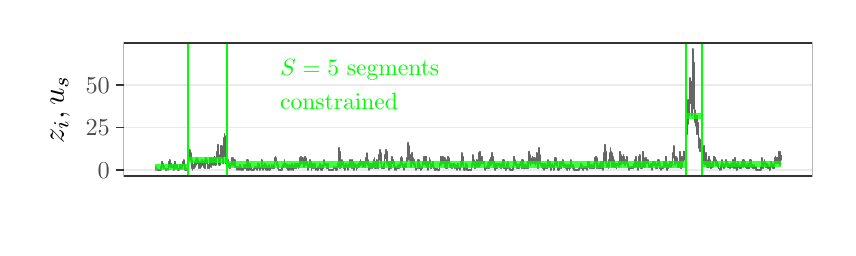
\begin{tikzpicture}[x=1pt,y=1pt]
\definecolor{fillColor}{RGB}{255,255,255}
\path[use as bounding box,fill=fillColor,fill opacity=0.00] (0,0) rectangle (289.08, 72.27);
\begin{scope}
\path[clip] (  0.00,  0.00) rectangle (289.08, 72.27);
\definecolor{drawColor}{RGB}{255,255,255}
\definecolor{fillColor}{RGB}{255,255,255}

\path[draw=drawColor,line width= 0.6pt,line join=round,line cap=round,fill=fillColor] (  0.00,  0.00) rectangle (289.08, 72.27);
\end{scope}
\begin{scope}
\path[clip] ( 34.65, 18.58) rectangle (283.58, 66.77);
\definecolor{fillColor}{RGB}{255,255,255}

\path[fill=fillColor] ( 34.65, 18.58) rectangle (283.58, 66.77);
\definecolor{drawColor}{gray}{0.92}

\path[draw=drawColor,line width= 0.6pt,line join=round] ( 34.65, 20.77) --
	(283.58, 20.77);

\path[draw=drawColor,line width= 0.6pt,line join=round] ( 34.65, 36.19) --
	(283.58, 36.19);

\path[draw=drawColor,line width= 0.6pt,line join=round] ( 34.65, 51.62) --
	(283.58, 51.62);
\definecolor{drawColor}{gray}{0.40}

\path[draw=drawColor,line width= 0.6pt,line join=round] ( 45.97, 21.38) --
	( 46.15, 21.38) --
	( 46.15, 20.77) --
	( 46.17, 20.77) --
	( 46.17, 21.38) --
	( 46.18, 21.38) --
	( 46.18, 22.00) --
	( 46.60, 22.00) --
	( 46.60, 21.38) --
	( 46.63, 21.38) --
	( 46.63, 20.77) --
	( 48.22, 20.77) --
	( 48.22, 21.38) --
	( 48.26, 21.38) --
	( 48.26, 22.00) --
	( 48.49, 22.00) --
	( 48.49, 22.62) --
	( 48.56, 22.62) --
	( 48.56, 23.23) --
	( 48.63, 23.23) --
	( 48.63, 23.85) --
	( 48.67, 23.85) --
	( 48.67, 23.23) --
	( 48.71, 23.23) --
	( 48.71, 22.62) --
	( 48.83, 22.62) --
	( 48.83, 23.23) --
	( 48.94, 23.23) --
	( 48.94, 22.62) --
	( 49.00, 22.62) --
	( 49.00, 23.23) --
	( 49.01, 23.23) --
	( 49.01, 22.62) --
	( 49.08, 22.62) --
	( 49.08, 22.00) --
	( 49.29, 22.00) --
	( 49.29, 21.38) --
	( 49.31, 21.38) --
	( 49.31, 22.00) --
	( 49.45, 22.00) --
	( 49.45, 21.38) --
	( 49.76, 21.38) --
	( 49.76, 20.77) --
	( 50.20, 20.77) --
	( 50.20, 21.38) --
	( 50.65, 21.38) --
	( 50.65, 20.77) --
	( 50.68, 20.77) --
	( 50.68, 21.38) --
	( 50.86, 21.38) --
	( 50.86, 22.00) --
	( 50.96, 22.00) --
	( 50.96, 22.62) --
	( 51.04, 22.62) --
	( 51.04, 23.23) --
	( 51.06, 23.23) --
	( 51.06, 23.85) --
	( 51.14, 23.85) --
	( 51.14, 23.23) --
	( 51.20, 23.23) --
	( 51.20, 23.85) --
	( 51.30, 23.85) --
	( 51.30, 24.47) --
	( 51.31, 24.47) --
	( 51.31, 23.85) --
	( 51.32, 23.85) --
	( 51.32, 24.47) --
	( 51.41, 24.47) --
	( 51.41, 23.85) --
	( 51.47, 23.85) --
	( 51.47, 24.47) --
	( 51.50, 24.47) --
	( 51.50, 23.85) --
	( 51.51, 23.85) --
	( 51.51, 23.23) --
	( 51.53, 23.23) --
	( 51.53, 23.85) --
	( 51.65, 23.85) --
	( 51.65, 23.23) --
	( 51.75, 23.23) --
	( 51.75, 22.62) --
	( 51.77, 22.62) --
	( 51.77, 22.00) --
	( 51.80, 22.00) --
	( 51.80, 22.62) --
	( 51.82, 22.62) --
	( 51.82, 23.23) --
	( 51.93, 23.23) --
	( 51.93, 22.62) --
	( 51.97, 22.62) --
	( 51.97, 22.00) --
	( 52.26, 22.00) --
	( 52.26, 22.62) --
	( 52.27, 22.62) --
	( 52.27, 22.00) --
	( 52.70, 22.00) --
	( 52.70, 20.77) --
	( 52.81, 20.77) --
	( 52.81, 21.38) --
	( 52.83, 21.38) --
	( 52.83, 22.00) --
	( 52.88, 22.00) --
	( 52.88, 22.62) --
	( 53.02, 22.62) --
	( 53.02, 23.23) --
	( 53.10, 23.23) --
	( 53.10, 23.85) --
	( 53.26, 23.85) --
	( 53.26, 23.23) --
	( 53.29, 23.23) --
	( 53.29, 22.62) --
	( 53.34, 22.62) --
	( 53.34, 22.00) --
	( 53.34, 22.00) --
	( 53.34, 22.62) --
	( 53.47, 22.62) --
	( 53.47, 22.00) --
	( 53.55, 22.00) --
	( 53.55, 21.38) --
	( 53.60, 21.38) --
	( 53.60, 22.00) --
	( 53.69, 22.00) --
	( 53.69, 22.62) --
	( 53.79, 22.62) --
	( 53.79, 22.00) --
	( 53.98, 22.00) --
	( 53.98, 22.62) --
	( 54.05, 22.62) --
	( 54.05, 22.00) --
	( 54.14, 22.00) --
	( 54.14, 21.38) --
	( 54.43, 21.38) --
	( 54.43, 20.77) --
	( 54.79, 20.77) --
	( 54.79, 21.38) --
	( 55.03, 21.38) --
	( 55.03, 22.00) --
	( 55.09, 22.00) --
	( 55.09, 22.62) --
	( 55.25, 22.62) --
	( 55.25, 22.00) --
	( 55.35, 22.00) --
	( 55.35, 22.62) --
	( 55.48, 22.62) --
	( 55.48, 22.00) --
	( 55.54, 22.00) --
	( 55.54, 21.38) --
	( 55.78, 21.38) --
	( 55.78, 22.00) --
	( 55.80, 22.00) --
	( 55.80, 21.38) --
	( 55.81, 21.38) --
	( 55.81, 22.00) --
	( 55.98, 22.00) --
	( 55.98, 23.23) --
	( 56.17, 23.23) --
	( 56.17, 23.85) --
	( 56.23, 23.85) --
	( 56.23, 23.23) --
	( 56.27, 23.23) --
	( 56.27, 22.62) --
	( 56.41, 22.62) --
	( 56.41, 23.85) --
	( 56.43, 23.85) --
	( 56.43, 24.47) --
	( 56.44, 24.47) --
	( 56.44, 23.23) --
	( 56.62, 23.23) --
	( 56.62, 22.62) --
	( 56.87, 22.62) --
	( 56.87, 21.38) --
	( 56.87, 21.38) --
	( 56.87, 20.77) --
	( 57.13, 20.77) --
	( 57.13, 21.38) --
	( 57.59, 21.38) --
	( 57.59, 20.77) --
	( 57.72, 20.77) --
	( 57.72, 21.38) --
	( 57.77, 21.38) --
	( 57.77, 22.00) --
	( 57.82, 22.00) --
	( 57.82, 23.23) --
	( 57.91, 23.23) --
	( 57.91, 24.47) --
	( 58.05, 24.47) --
	( 58.05, 25.09) --
	( 58.10, 25.09) --
	( 58.10, 25.70) --
	( 58.17, 25.70) --
	( 58.17, 25.09) --
	( 58.20, 25.09) --
	( 58.20, 26.94) --
	( 58.22, 26.94) --
	( 58.22, 27.55) --
	( 58.22, 27.55) --
	( 58.22, 26.94) --
	( 58.27, 26.94) --
	( 58.27, 28.17) --
	( 58.27, 28.17) --
	( 58.27, 26.94) --
	( 58.34, 26.94) --
	( 58.34, 27.55) --
	( 58.37, 27.55) --
	( 58.37, 26.32) --
	( 58.43, 26.32) --
	( 58.43, 26.94) --
	( 58.51, 26.94) --
	( 58.51, 26.32) --
	( 58.56, 26.32) --
	( 58.56, 25.70) --
	( 58.59, 25.70) --
	( 58.59, 27.55) --
	( 58.64, 27.55) --
	( 58.64, 28.17) --
	( 58.65, 28.17) --
	( 58.65, 27.55) --
	( 58.65, 27.55) --
	( 58.65, 26.32) --
	( 58.67, 26.32) --
	( 58.67, 25.70) --
	( 58.73, 25.70) --
	( 58.73, 24.47) --
	( 58.81, 24.47) --
	( 58.81, 25.09) --
	( 58.84, 25.09) --
	( 58.84, 25.70) --
	( 58.84, 25.70) --
	( 58.84, 26.32) --
	( 58.89, 26.32) --
	( 58.89, 25.70) --
	( 58.99, 25.70) --
	( 58.99, 26.32) --
	( 59.02, 26.32) --
	( 59.02, 26.94) --
	( 59.04, 26.94) --
	( 59.04, 25.09) --
	( 59.05, 25.09) --
	( 59.05, 25.70) --
	( 59.09, 25.70) --
	( 59.09, 25.09) --
	( 59.25, 25.09) --
	( 59.25, 24.47) --
	( 59.27, 24.47) --
	( 59.27, 23.85) --
	( 59.29, 23.85) --
	( 59.29, 22.62) --
	( 59.45, 22.62) --
	( 59.45, 21.38) --
	( 59.51, 21.38) --
	( 59.51, 20.77) --
	( 59.56, 20.77) --
	( 59.56, 21.38) --
	( 59.65, 21.38) --
	( 59.65, 22.00) --
	( 59.87, 22.00) --
	( 59.87, 22.62) --
	( 60.00, 22.62) --
	( 60.00, 22.00) --
	( 60.10, 22.00) --
	( 60.10, 21.38) --
	( 60.22, 21.38) --
	( 60.22, 22.00) --
	( 60.32, 22.00) --
	( 60.32, 21.38) --
	( 60.33, 21.38) --
	( 60.33, 22.00) --
	( 60.37, 22.00) --
	( 60.37, 22.62) --
	( 60.39, 22.62) --
	( 60.39, 23.23) --
	( 60.56, 23.23) --
	( 60.56, 23.85) --
	( 60.67, 23.85) --
	( 60.67, 23.23) --
	( 60.69, 23.23) --
	( 60.69, 23.85) --
	( 60.78, 23.85) --
	( 60.78, 23.23) --
	( 60.82, 23.23) --
	( 60.82, 22.62) --
	( 60.83, 22.62) --
	( 60.83, 23.85) --
	( 60.85, 23.85) --
	( 60.85, 23.23) --
	( 60.92, 23.23) --
	( 60.92, 23.85) --
	( 60.94, 23.85) --
	( 60.94, 24.47) --
	( 61.09, 24.47) --
	( 61.09, 25.09) --
	( 61.14, 25.09) --
	( 61.14, 24.47) --
	( 61.23, 24.47) --
	( 61.23, 25.09) --
	( 61.28, 25.09) --
	( 61.28, 23.85) --
	( 61.37, 23.85) --
	( 61.37, 24.47) --
	( 61.38, 24.47) --
	( 61.38, 23.85) --
	( 61.39, 23.85) --
	( 61.39, 23.23) --
	( 61.42, 23.23) --
	( 61.42, 24.47) --
	( 61.46, 24.47) --
	( 61.46, 23.85) --
	( 61.54, 23.85) --
	( 61.54, 23.23) --
	( 61.68, 23.23) --
	( 61.68, 22.62) --
	( 61.79, 22.62) --
	( 61.79, 23.23) --
	( 61.82, 23.23) --
	( 61.82, 22.62) --
	( 61.88, 22.62) --
	( 61.88, 21.38) --
	( 61.89, 21.38) --
	( 61.89, 22.00) --
	( 61.91, 22.00) --
	( 61.91, 22.62) --
	( 61.96, 22.62) --
	( 61.96, 23.23) --
	( 62.22, 23.23) --
	( 62.22, 23.85) --
	( 62.23, 23.85) --
	( 62.23, 23.23) --
	( 62.34, 23.23) --
	( 62.34, 22.62) --
	( 62.36, 22.62) --
	( 62.36, 22.00) --
	( 62.42, 22.00) --
	( 62.42, 21.38) --
	( 62.50, 21.38) --
	( 62.50, 22.00) --
	( 62.61, 22.00) --
	( 62.61, 22.62) --
	( 62.63, 22.62) --
	( 62.63, 23.23) --
	( 62.64, 23.23) --
	( 62.64, 23.85) --
	( 62.66, 23.85) --
	( 62.66, 23.23) --
	( 62.68, 23.23) --
	( 62.68, 23.85) --
	( 62.75, 23.85) --
	( 62.75, 24.47) --
	( 62.95, 24.47) --
	( 62.95, 23.85) --
	( 63.03, 23.85) --
	( 63.03, 24.47) --
	( 63.09, 24.47) --
	( 63.09, 23.85) --
	( 63.09, 23.85) --
	( 63.09, 23.23) --
	( 63.10, 23.23) --
	( 63.10, 23.85) --
	( 63.14, 23.85) --
	( 63.14, 23.23) --
	( 63.20, 23.23) --
	( 63.20, 22.62) --
	( 63.42, 22.62) --
	( 63.42, 23.23) --
	( 63.45, 23.23) --
	( 63.45, 23.85) --
	( 63.48, 23.85) --
	( 63.48, 23.23) --
	( 63.51, 23.23) --
	( 63.51, 22.62) --
	( 63.55, 22.62) --
	( 63.55, 22.00) --
	( 63.86, 22.00) --
	( 63.86, 22.62) --
	( 63.87, 22.62) --
	( 63.87, 22.00) --
	( 63.91, 22.00) --
	( 63.91, 21.38) --
	( 63.96, 21.38) --
	( 63.96, 22.00) --
	( 63.97, 22.00) --
	( 63.97, 22.62) --
	( 64.06, 22.62) --
	( 64.06, 23.23) --
	( 64.14, 23.23) --
	( 64.14, 23.85) --
	( 64.17, 23.85) --
	( 64.17, 24.47) --
	( 64.25, 24.47) --
	( 64.25, 25.09) --
	( 64.31, 25.09) --
	( 64.31, 24.47) --
	( 64.39, 24.47) --
	( 64.39, 25.09) --
	( 64.41, 25.09) --
	( 64.41, 24.47) --
	( 64.42, 24.47) --
	( 64.42, 23.85) --
	( 64.48, 23.85) --
	( 64.48, 23.23) --
	( 64.52, 23.23) --
	( 64.52, 23.85) --
	( 64.58, 23.85) --
	( 64.58, 24.47) --
	( 64.59, 24.47) --
	( 64.59, 23.85) --
	( 64.60, 23.85) --
	( 64.60, 24.47) --
	( 64.62, 24.47) --
	( 64.62, 23.85) --
	( 64.65, 23.85) --
	( 64.65, 24.47) --
	( 64.71, 24.47) --
	( 64.71, 23.85) --
	( 64.76, 23.85) --
	( 64.76, 24.47) --
	( 64.85, 24.47) --
	( 64.85, 23.85) --
	( 64.97, 23.85) --
	( 64.97, 23.23) --
	( 65.04, 23.23) --
	( 65.04, 22.62) --
	( 65.05, 22.62) --
	( 65.05, 22.00) --
	( 65.10, 22.00) --
	( 65.10, 21.38) --
	( 65.13, 21.38) --
	( 65.13, 22.00) --
	( 65.15, 22.00) --
	( 65.15, 21.38) --
	( 65.28, 21.38) --
	( 65.28, 22.00) --
	( 65.53, 22.00) --
	( 65.53, 22.62) --
	( 65.58, 22.62) --
	( 65.58, 22.00) --
	( 65.73, 22.00) --
	( 65.73, 21.38) --
	( 65.76, 21.38) --
	( 65.76, 22.62) --
	( 65.78, 22.62) --
	( 65.78, 23.23) --
	( 65.80, 23.23) --
	( 65.80, 23.85) --
	( 65.82, 23.85) --
	( 65.82, 24.47) --
	( 65.86, 24.47) --
	( 65.86, 25.09) --
	( 65.98, 25.09) --
	( 65.98, 24.47) --
	( 66.05, 24.47) --
	( 66.05, 25.09) --
	( 66.21, 25.09) --
	( 66.21, 23.85) --
	( 66.24, 23.85) --
	( 66.24, 23.23) --
	( 66.24, 23.23) --
	( 66.24, 22.62) --
	( 66.31, 22.62) --
	( 66.31, 22.00) --
	( 66.39, 22.00) --
	( 66.39, 22.62) --
	( 66.41, 22.62) --
	( 66.41, 23.85) --
	( 66.53, 23.85) --
	( 66.53, 24.47) --
	( 66.58, 24.47) --
	( 66.58, 25.09) --
	( 66.72, 25.09) --
	( 66.72, 24.47) --
	( 66.84, 24.47) --
	( 66.84, 23.85) --
	( 66.86, 23.85) --
	( 66.86, 22.62) --
	( 66.89, 22.62) --
	( 66.89, 23.23) --
	( 66.96, 23.23) --
	( 66.96, 22.62) --
	( 66.98, 22.62) --
	( 66.98, 23.23) --
	( 66.99, 23.23) --
	( 66.99, 22.62) --
	( 67.02, 22.62) --
	( 67.02, 23.23) --
	( 67.03, 23.23) --
	( 67.03, 22.62) --
	( 67.09, 22.62) --
	( 67.09, 23.23) --
	( 67.16, 23.23) --
	( 67.16, 23.85) --
	( 67.19, 23.85) --
	( 67.19, 24.47) --
	( 67.27, 24.47) --
	( 67.27, 25.09) --
	( 67.34, 25.09) --
	( 67.34, 24.47) --
	( 67.34, 24.47) --
	( 67.34, 25.09) --
	( 67.43, 25.09) --
	( 67.43, 24.47) --
	( 67.46, 24.47) --
	( 67.46, 25.09) --
	( 67.47, 25.09) --
	( 67.47, 25.70) --
	( 67.48, 25.70) --
	( 67.48, 25.09) --
	( 67.54, 25.09) --
	( 67.54, 24.47) --
	( 67.62, 24.47) --
	( 67.62, 23.85) --
	( 67.64, 23.85) --
	( 67.64, 23.23) --
	( 67.72, 23.23) --
	( 67.72, 22.62) --
	( 67.73, 22.62) --
	( 67.73, 23.23) --
	( 67.76, 23.23) --
	( 67.76, 24.47) --
	( 67.80, 24.47) --
	( 67.80, 23.85) --
	( 67.91, 23.85) --
	( 67.91, 23.23) --
	( 67.92, 23.23) --
	( 67.92, 22.62) --
	( 67.94, 22.62) --
	( 67.94, 23.23) --
	( 67.99, 23.23) --
	( 67.99, 23.85) --
	( 68.06, 23.85) --
	( 68.06, 24.47) --
	( 68.16, 24.47) --
	( 68.16, 25.09) --
	( 68.18, 25.09) --
	( 68.18, 24.47) --
	( 68.20, 24.47) --
	( 68.20, 25.09) --
	( 68.20, 25.09) --
	( 68.20, 25.70) --
	( 68.21, 25.70) --
	( 68.21, 25.09) --
	( 68.21, 25.09) --
	( 68.21, 24.47) --
	( 68.24, 24.47) --
	( 68.24, 25.09) --
	( 68.39, 25.09) --
	( 68.39, 25.70) --
	( 68.39, 25.70) --
	( 68.39, 25.09) --
	( 68.44, 25.09) --
	( 68.44, 25.70) --
	( 68.44, 25.70) --
	( 68.44, 25.09) --
	( 68.46, 25.09) --
	( 68.46, 26.94) --
	( 68.47, 26.94) --
	( 68.47, 27.55) --
	( 68.49, 27.55) --
	( 68.49, 26.94) --
	( 68.51, 26.94) --
	( 68.51, 27.55) --
	( 68.56, 27.55) --
	( 68.56, 28.17) --
	( 68.60, 28.17) --
	( 68.60, 28.79) --
	( 68.61, 28.79) --
	( 68.61, 28.17) --
	( 68.65, 28.17) --
	( 68.65, 27.55) --
	( 68.66, 27.55) --
	( 68.66, 26.94) --
	( 68.66, 26.94) --
	( 68.66, 27.55) --
	( 68.69, 27.55) --
	( 68.69, 28.17) --
	( 68.69, 28.17) --
	( 68.69, 27.55) --
	( 68.70, 27.55) --
	( 68.70, 28.79) --
	( 68.77, 28.79) --
	( 68.77, 29.41) --
	( 68.83, 29.41) --
	( 68.83, 30.02) --
	( 68.83, 30.02) --
	( 68.83, 29.41) --
	( 68.89, 29.41) --
	( 68.89, 28.79) --
	( 68.92, 28.79) --
	( 68.92, 26.94) --
	( 68.92, 26.94) --
	( 68.92, 25.70) --
	( 68.93, 25.70) --
	( 68.93, 26.32) --
	( 68.99, 26.32) --
	( 68.99, 26.94) --
	( 69.01, 26.94) --
	( 69.01, 26.32) --
	( 69.05, 26.32) --
	( 69.05, 25.70) --
	( 69.06, 25.70) --
	( 69.06, 25.09) --
	( 69.14, 25.09) --
	( 69.14, 24.47) --
	( 69.16, 24.47) --
	( 69.16, 23.23) --
	( 69.20, 23.23) --
	( 69.20, 23.85) --
	( 69.21, 23.85) --
	( 69.21, 22.62) --
	( 69.30, 22.62) --
	( 69.30, 23.23) --
	( 69.38, 23.23) --
	( 69.38, 23.85) --
	( 69.39, 23.85) --
	( 69.39, 23.23) --
	( 69.44, 23.23) --
	( 69.44, 22.62) --
	( 69.51, 22.62) --
	( 69.51, 23.85) --
	( 69.55, 23.85) --
	( 69.55, 24.47) --
	( 69.59, 24.47) --
	( 69.59, 25.09) --
	( 69.59, 25.09) --
	( 69.59, 24.47) --
	( 69.66, 24.47) --
	( 69.66, 25.09) --
	( 69.68, 25.09) --
	( 69.68, 25.70) --
	( 69.75, 25.70) --
	( 69.75, 25.09) --
	( 69.78, 25.09) --
	( 69.78, 25.70) --
	( 69.79, 25.70) --
	( 69.79, 26.32) --
	( 69.82, 26.32) --
	( 69.82, 26.94) --
	( 69.85, 26.94) --
	( 69.85, 26.32) --
	( 69.87, 26.32) --
	( 69.87, 26.94) --
	( 69.90, 26.94) --
	( 69.90, 27.55) --
	( 69.92, 27.55) --
	( 69.92, 28.17) --
	( 69.92, 28.17) --
	( 69.92, 28.79) --
	( 69.97, 28.79) --
	( 69.97, 29.41) --
	( 70.00, 29.41) --
	( 70.00, 28.79) --
	( 70.02, 28.79) --
	( 70.02, 29.41) --
	( 70.04, 29.41) --
	( 70.04, 28.79) --
	( 70.05, 28.79) --
	( 70.05, 28.17) --
	( 70.08, 28.17) --
	( 70.08, 28.79) --
	( 70.09, 28.79) --
	( 70.09, 29.41) --
	( 70.11, 29.41) --
	( 70.11, 28.79) --
	( 70.19, 28.79) --
	( 70.19, 29.41) --
	( 70.24, 29.41) --
	( 70.24, 28.79) --
	( 70.27, 28.79) --
	( 70.27, 28.17) --
	( 70.28, 28.17) --
	( 70.28, 28.79) --
	( 70.29, 28.79) --
	( 70.29, 28.17) --
	( 70.32, 28.17) --
	( 70.32, 28.79) --
	( 70.35, 28.79) --
	( 70.35, 28.17) --
	( 70.37, 28.17) --
	( 70.37, 27.55) --
	( 70.38, 27.55) --
	( 70.38, 26.94) --
	( 70.41, 26.94) --
	( 70.41, 26.32) --
	( 70.43, 26.32) --
	( 70.43, 25.70) --
	( 70.47, 25.70) --
	( 70.47, 25.09) --
	( 70.52, 25.09) --
	( 70.52, 24.47) --
	( 70.53, 24.47) --
	( 70.53, 25.09) --
	( 70.54, 25.09) --
	( 70.54, 24.47) --
	( 70.54, 24.47) --
	( 70.54, 23.85) --
	( 70.59, 23.85) --
	( 70.59, 23.23) --
	( 70.60, 23.23) --
	( 70.60, 23.85) --
	( 70.63, 23.85) --
	( 70.63, 24.47) --
	( 70.64, 24.47) --
	( 70.64, 23.85) --
	( 70.72, 23.85) --
	( 70.72, 24.47) --
	( 70.73, 24.47) --
	( 70.73, 23.85) --
	( 70.77, 23.85) --
	( 70.77, 23.23) --
	( 70.79, 23.23) --
	( 70.79, 23.85) --
	( 70.79, 23.85) --
	( 70.79, 25.09) --
	( 70.80, 25.09) --
	( 70.80, 25.70) --
	( 70.86, 25.70) --
	( 70.86, 26.32) --
	( 70.89, 26.32) --
	( 70.89, 26.94) --
	( 70.91, 26.94) --
	( 70.91, 27.55) --
	( 70.91, 27.55) --
	( 70.91, 28.17) --
	( 70.95, 28.17) --
	( 70.95, 28.79) --
	( 70.97, 28.79) --
	( 70.97, 29.41) --
	( 70.98, 29.41) --
	( 70.98, 28.79) --
	( 70.98, 28.79) --
	( 70.98, 29.41) --
	( 71.00, 29.41) --
	( 71.00, 31.26) --
	( 71.02, 31.26) --
	( 71.02, 31.87) --
	( 71.04, 31.87) --
	( 71.04, 31.26) --
	( 71.05, 31.26) --
	( 71.05, 31.87) --
	( 71.06, 31.87) --
	( 71.06, 32.49) --
	( 71.07, 32.49) --
	( 71.07, 33.11) --
	( 71.08, 33.11) --
	( 71.08, 33.73) --
	( 71.09, 33.73) --
	( 71.09, 33.11) --
	( 71.14, 33.11) --
	( 71.14, 33.73) --
	( 71.17, 33.73) --
	( 71.17, 33.11) --
	( 71.24, 33.11) --
	( 71.24, 32.49) --
	( 71.25, 32.49) --
	( 71.25, 31.87) --
	( 71.26, 31.87) --
	( 71.26, 31.26) --
	( 71.31, 31.26) --
	( 71.31, 30.64) --
	( 71.35, 30.64) --
	( 71.35, 30.02) --
	( 71.36, 30.02) --
	( 71.36, 29.41) --
	( 71.36, 29.41) --
	( 71.36, 28.79) --
	( 71.40, 28.79) --
	( 71.40, 28.17) --
	( 71.42, 28.17) --
	( 71.42, 27.55) --
	( 71.44, 27.55) --
	( 71.44, 26.94) --
	( 71.45, 26.94) --
	( 71.45, 25.09) --
	( 71.46, 25.09) --
	( 71.46, 25.70) --
	( 71.47, 25.70) --
	( 71.47, 24.47) --
	( 71.50, 24.47) --
	( 71.50, 23.85) --
	( 71.51, 23.85) --
	( 71.51, 23.23) --
	( 71.52, 23.23) --
	( 71.52, 23.85) --
	( 71.53, 23.85) --
	( 71.53, 24.47) --
	( 71.54, 24.47) --
	( 71.54, 23.85) --
	( 71.59, 23.85) --
	( 71.59, 23.23) --
	( 71.71, 23.23) --
	( 71.71, 24.47) --
	( 71.91, 24.47) --
	( 71.91, 23.85) --
	( 71.97, 23.85) --
	( 71.97, 22.00) --
	( 72.14, 22.00) --
	( 72.14, 23.23) --
	( 72.16, 23.23) --
	( 72.16, 22.00) --
	( 72.25, 22.00) --
	( 72.25, 22.62) --
	( 72.38, 22.62) --
	( 72.38, 23.23) --
	( 72.52, 23.23) --
	( 72.52, 23.85) --
	( 72.53, 23.85) --
	( 72.53, 24.47) --
	( 72.59, 24.47) --
	( 72.59, 23.23) --
	( 72.69, 23.23) --
	( 72.69, 22.62) --
	( 72.83, 22.62) --
	( 72.83, 22.00) --
	( 72.84, 22.00) --
	( 72.84, 22.62) --
	( 72.97, 22.62) --
	( 72.97, 22.00) --
	( 72.98, 22.00) --
	( 72.98, 21.38) --
	( 73.00, 21.38) --
	( 73.00, 22.00) --
	( 73.01, 22.00) --
	( 73.01, 22.62) --
	( 73.28, 22.62) --
	( 73.28, 23.23) --
	( 73.29, 23.23) --
	( 73.29, 22.62) --
	( 73.43, 22.62) --
	( 73.43, 23.23) --
	( 73.46, 23.23) --
	( 73.46, 22.62) --
	( 73.53, 22.62) --
	( 73.53, 23.23) --
	( 73.66, 23.23) --
	( 73.66, 23.85) --
	( 73.73, 23.85) --
	( 73.73, 23.23) --
	( 73.77, 23.23) --
	( 73.77, 23.85) --
	( 73.83, 23.85) --
	( 73.83, 25.09) --
	( 73.88, 25.09) --
	( 73.88, 24.47) --
	( 73.91, 24.47) --
	( 73.91, 23.85) --
	( 73.98, 23.85) --
	( 73.98, 23.23) --
	( 74.03, 23.23) --
	( 74.03, 23.85) --
	( 74.05, 23.85) --
	( 74.05, 24.47) --
	( 74.11, 24.47) --
	( 74.11, 23.85) --
	( 74.16, 23.85) --
	( 74.16, 24.47) --
	( 74.20, 24.47) --
	( 74.20, 25.09) --
	( 74.21, 25.09) --
	( 74.21, 24.47) --
	( 74.21, 24.47) --
	( 74.21, 23.85) --
	( 74.24, 23.85) --
	( 74.24, 23.23) --
	( 74.28, 23.23) --
	( 74.28, 22.62) --
	( 74.36, 22.62) --
	( 74.36, 23.23) --
	( 74.38, 23.23) --
	( 74.38, 23.85) --
	( 74.41, 23.85) --
	( 74.41, 23.23) --
	( 74.50, 23.23) --
	( 74.50, 22.62) --
	( 74.52, 22.62) --
	( 74.52, 23.23) --
	( 74.52, 23.23) --
	( 74.52, 23.85) --
	( 74.62, 23.85) --
	( 74.62, 24.47) --
	( 74.65, 24.47) --
	( 74.65, 23.85) --
	( 74.65, 23.85) --
	( 74.65, 24.47) --
	( 74.81, 24.47) --
	( 74.81, 23.85) --
	( 74.83, 23.85) --
	( 74.83, 23.23) --
	( 74.97, 23.23) --
	( 74.97, 22.00) --
	( 75.05, 22.00) --
	( 75.05, 22.62) --
	( 75.07, 22.62) --
	( 75.07, 22.00) --
	( 75.08, 22.00) --
	( 75.08, 22.62) --
	( 75.10, 22.62) --
	( 75.10, 22.00) --
	( 75.50, 22.00) --
	( 75.50, 21.38) --
	( 75.53, 21.38) --
	( 75.53, 20.77) --
	( 75.72, 20.77) --
	( 75.72, 21.38) --
	( 75.83, 21.38) --
	( 75.83, 22.00) --
	( 76.12, 22.00) --
	( 76.12, 21.38) --
	( 76.28, 21.38) --
	( 76.28, 20.77) --
	( 76.47, 20.77) --
	( 76.47, 21.38) --
	( 76.53, 21.38) --
	( 76.53, 22.00) --
	( 76.54, 22.00) --
	( 76.54, 22.62) --
	( 76.92, 22.62) --
	( 76.92, 22.00) --
	( 76.98, 22.00) --
	( 76.98, 21.38) --
	( 76.99, 21.38) --
	( 76.99, 20.77) --
	( 77.22, 20.77) --
	( 77.22, 21.38) --
	( 77.68, 21.38) --
	( 77.68, 20.77) --
	( 77.89, 20.77) --
	( 77.89, 21.38) --
	( 78.03, 21.38) --
	( 78.03, 22.00) --
	( 78.20, 22.00) --
	( 78.20, 22.62) --
	( 78.24, 22.62) --
	( 78.24, 22.00) --
	( 78.35, 22.00) --
	( 78.35, 21.38) --
	( 78.51, 21.38) --
	( 78.51, 22.00) --
	( 78.57, 22.00) --
	( 78.57, 22.62) --
	( 78.65, 22.62) --
	( 78.65, 22.00) --
	( 78.96, 22.00) --
	( 78.96, 21.38) --
	( 79.02, 21.38) --
	( 79.02, 20.77) --
	( 79.20, 20.77) --
	( 79.20, 22.62) --
	( 79.23, 22.62) --
	( 79.23, 24.47) --
	( 79.65, 24.47) --
	( 79.65, 22.62) --
	( 79.68, 22.62) --
	( 79.68, 22.00) --
	( 79.68, 22.00) --
	( 79.68, 20.77) --
	( 79.93, 20.77) --
	( 79.93, 21.38) --
	( 79.96, 21.38) --
	( 79.96, 22.00) --
	( 80.14, 22.00) --
	( 80.14, 22.62) --
	( 80.29, 22.62) --
	( 80.29, 23.23) --
	( 80.35, 23.23) --
	( 80.35, 22.62) --
	( 80.41, 22.62) --
	( 80.41, 22.00) --
	( 80.59, 22.00) --
	( 80.59, 21.38) --
	( 80.74, 21.38) --
	( 80.74, 20.77) --
	( 81.79, 20.77) --
	( 81.79, 21.38) --
	( 82.03, 21.38) --
	( 82.03, 22.00) --
	( 82.24, 22.00) --
	( 82.24, 21.38) --
	( 82.27, 21.38) --
	( 82.27, 22.00) --
	( 82.48, 22.00) --
	( 82.48, 21.38) --
	( 82.53, 21.38) --
	( 82.53, 22.00) --
	( 82.72, 22.00) --
	( 82.72, 21.38) --
	( 82.98, 21.38) --
	( 82.98, 20.77) --
	( 83.02, 20.77) --
	( 83.02, 21.38) --
	( 83.25, 21.38) --
	( 83.25, 22.00) --
	( 83.28, 22.00) --
	( 83.28, 22.62) --
	( 83.29, 22.62) --
	( 83.29, 23.23) --
	( 83.47, 23.23) --
	( 83.47, 22.62) --
	( 83.71, 22.62) --
	( 83.71, 22.00) --
	( 83.73, 22.00) --
	( 83.73, 21.38) --
	( 83.74, 21.38) --
	( 83.74, 20.77) --
	( 83.85, 20.77) --
	( 83.85, 21.38) --
	( 84.23, 21.38) --
	( 84.23, 22.00) --
	( 84.30, 22.00) --
	( 84.30, 21.38) --
	( 84.38, 21.38) --
	( 84.38, 22.00) --
	( 84.46, 22.00) --
	( 84.46, 22.62) --
	( 84.49, 22.62) --
	( 84.49, 23.85) --
	( 84.51, 23.85) --
	( 84.51, 24.47) --
	( 84.68, 24.47) --
	( 84.68, 23.85) --
	( 84.83, 23.85) --
	( 84.83, 23.23) --
	( 84.91, 23.23) --
	( 84.91, 22.62) --
	( 84.95, 22.62) --
	( 84.95, 21.38) --
	( 84.96, 21.38) --
	( 84.96, 20.77) --
	( 84.99, 20.77) --
	( 84.99, 21.38) --
	( 85.22, 21.38) --
	( 85.22, 22.00) --
	( 85.44, 22.00) --
	( 85.44, 21.38) --
	( 85.57, 21.38) --
	( 85.57, 22.00) --
	( 85.63, 22.00) --
	( 85.63, 23.23) --
	( 85.67, 23.23) --
	( 85.67, 22.62) --
	( 86.02, 22.62) --
	( 86.02, 22.00) --
	( 86.08, 22.00) --
	( 86.08, 20.77) --
	( 86.14, 20.77) --
	( 86.14, 21.38) --
	( 86.38, 21.38) --
	( 86.38, 22.00) --
	( 86.59, 22.00) --
	( 86.59, 20.77) --
	( 86.66, 20.77) --
	( 86.66, 21.38) --
	( 86.80, 21.38) --
	( 86.80, 22.00) --
	( 87.05, 22.00) --
	( 87.05, 22.62) --
	( 87.09, 22.62) --
	( 87.09, 22.00) --
	( 87.24, 22.00) --
	( 87.24, 20.77) --
	( 87.50, 20.77) --
	( 87.50, 21.38) --
	( 87.93, 21.38) --
	( 87.93, 22.00) --
	( 87.95, 22.00) --
	( 87.95, 21.38) --
	( 88.03, 21.38) --
	( 88.03, 22.00) --
	( 88.20, 22.00) --
	( 88.20, 22.62) --
	( 88.38, 22.62) --
	( 88.38, 22.00) --
	( 88.49, 22.00) --
	( 88.49, 21.38) --
	( 88.50, 21.38) --
	( 88.50, 22.00) --
	( 88.63, 22.00) --
	( 88.63, 21.38) --
	( 88.76, 21.38) --
	( 88.76, 22.00) --
	( 88.95, 22.00) --
	( 88.95, 21.38) --
	( 89.11, 21.38) --
	( 89.11, 22.00) --
	( 89.12, 22.00) --
	( 89.12, 22.62) --
	( 89.17, 22.62) --
	( 89.17, 23.85) --
	( 89.21, 23.85) --
	( 89.21, 23.23) --
	( 89.25, 23.23) --
	( 89.25, 23.85) --
	( 89.28, 23.85) --
	( 89.28, 24.47) --
	( 89.39, 24.47) --
	( 89.39, 25.09) --
	( 89.50, 25.09) --
	( 89.50, 25.70) --
	( 89.56, 25.70) --
	( 89.56, 25.09) --
	( 89.57, 25.09) --
	( 89.57, 25.70) --
	( 89.58, 25.70) --
	( 89.58, 25.09) --
	( 89.63, 25.09) --
	( 89.63, 23.85) --
	( 89.69, 23.85) --
	( 89.69, 24.47) --
	( 89.70, 24.47) --
	( 89.70, 23.85) --
	( 89.71, 23.85) --
	( 89.71, 24.47) --
	( 89.73, 24.47) --
	( 89.73, 23.85) --
	( 89.81, 23.85) --
	( 89.81, 24.47) --
	( 89.84, 24.47) --
	( 89.84, 23.85) --
	( 89.95, 23.85) --
	( 89.95, 23.23) --
	( 89.99, 23.23) --
	( 89.99, 23.85) --
	( 90.02, 23.85) --
	( 90.02, 23.23) --
	( 90.08, 23.23) --
	( 90.08, 23.85) --
	( 90.15, 23.85) --
	( 90.15, 23.23) --
	( 90.15, 23.23) --
	( 90.15, 22.62) --
	( 90.22, 22.62) --
	( 90.22, 23.23) --
	( 90.26, 23.23) --
	( 90.26, 22.62) --
	( 90.44, 22.62) --
	( 90.44, 22.00) --
	( 90.54, 22.00) --
	( 90.54, 21.38) --
	( 90.68, 21.38) --
	( 90.68, 20.77) --
	( 91.91, 20.77) --
	( 91.91, 21.38) --
	( 91.93, 21.38) --
	( 91.93, 22.00) --
	( 92.07, 22.00) --
	( 92.07, 22.62) --
	( 92.35, 22.62) --
	( 92.35, 22.00) --
	( 92.36, 22.00) --
	( 92.36, 22.62) --
	( 92.38, 22.62) --
	( 92.38, 23.23) --
	( 92.39, 23.23) --
	( 92.39, 22.62) --
	( 92.53, 22.62) --
	( 92.53, 22.00) --
	( 92.61, 22.00) --
	( 92.61, 22.62) --
	( 92.69, 22.62) --
	( 92.69, 23.23) --
	( 92.79, 23.23) --
	( 92.79, 24.47) --
	( 92.81, 24.47) --
	( 92.81, 23.85) --
	( 92.83, 23.85) --
	( 92.83, 23.23) --
	( 93.07, 23.23) --
	( 93.07, 22.62) --
	( 93.11, 22.62) --
	( 93.11, 23.23) --
	( 93.14, 23.23) --
	( 93.14, 22.62) --
	( 93.16, 22.62) --
	( 93.16, 23.23) --
	( 93.24, 23.23) --
	( 93.24, 22.00) --
	( 93.52, 22.00) --
	( 93.52, 22.62) --
	( 93.56, 22.62) --
	( 93.56, 22.00) --
	( 93.61, 22.00) --
	( 93.61, 21.38) --
	( 93.64, 21.38) --
	( 93.64, 22.00) --
	( 93.72, 22.00) --
	( 93.72, 22.62) --
	( 93.97, 22.62) --
	( 93.97, 22.00) --
	( 94.09, 22.00) --
	( 94.09, 21.38) --
	( 94.17, 21.38) --
	( 94.17, 20.77) --
	( 94.42, 20.77) --
	( 94.42, 21.38) --
	( 94.42, 21.38) --
	( 94.42, 22.00) --
	( 94.75, 22.00) --
	( 94.75, 22.62) --
	( 94.87, 22.62) --
	( 94.87, 21.38) --
	( 95.20, 21.38) --
	( 95.20, 20.77) --
	( 95.22, 20.77) --
	( 95.22, 21.38) --
	( 95.39, 21.38) --
	( 95.39, 22.00) --
	( 95.47, 22.00) --
	( 95.47, 22.62) --
	( 95.50, 22.62) --
	( 95.50, 23.23) --
	( 95.67, 23.23) --
	( 95.67, 22.62) --
	( 95.84, 22.62) --
	( 95.84, 22.00) --
	( 95.92, 22.00) --
	( 95.92, 21.38) --
	( 95.95, 21.38) --
	( 95.95, 20.77) --
	( 96.00, 20.77) --
	( 96.00, 21.38) --
	( 96.37, 21.38) --
	( 96.37, 22.00) --
	( 96.44, 22.00) --
	( 96.44, 22.62) --
	( 96.45, 22.62) --
	( 96.45, 22.00) --
	( 96.46, 22.00) --
	( 96.46, 22.62) --
	( 96.56, 22.62) --
	( 96.56, 23.23) --
	( 96.82, 23.23) --
	( 96.82, 22.62) --
	( 96.84, 22.62) --
	( 96.84, 23.23) --
	( 96.89, 23.23) --
	( 96.89, 22.62) --
	( 96.90, 22.62) --
	( 96.90, 22.00) --
	( 97.01, 22.00) --
	( 97.01, 21.38) --
	( 97.14, 21.38) --
	( 97.14, 22.00) --
	( 97.22, 22.00) --
	( 97.22, 22.62) --
	( 97.30, 22.62) --
	( 97.30, 22.00) --
	( 97.36, 22.00) --
	( 97.36, 22.62) --
	( 97.44, 22.62) --
	( 97.44, 23.23) --
	( 97.58, 23.23) --
	( 97.58, 22.62) --
	( 97.60, 22.62) --
	( 97.60, 23.23) --
	( 97.67, 23.23) --
	( 97.67, 22.62) --
	( 97.81, 22.62) --
	( 97.81, 22.00) --
	( 97.89, 22.00) --
	( 97.89, 21.38) --
	( 97.92, 21.38) --
	( 97.92, 22.00) --
	( 97.95, 22.00) --
	( 97.95, 22.62) --
	( 98.06, 22.62) --
	( 98.06, 22.00) --
	( 98.11, 22.00) --
	( 98.11, 22.62) --
	( 98.19, 22.62) --
	( 98.19, 22.00) --
	( 98.21, 22.00) --
	( 98.21, 22.62) --
	( 98.32, 22.62) --
	( 98.32, 23.23) --
	( 98.36, 23.23) --
	( 98.36, 23.85) --
	( 98.42, 23.85) --
	( 98.42, 24.47) --
	( 98.51, 24.47) --
	( 98.51, 25.09) --
	( 98.56, 25.09) --
	( 98.56, 24.47) --
	( 98.65, 24.47) --
	( 98.65, 23.85) --
	( 98.70, 23.85) --
	( 98.70, 24.47) --
	( 98.70, 24.47) --
	( 98.70, 25.09) --
	( 98.76, 25.09) --
	( 98.76, 25.70) --
	( 98.77, 25.70) --
	( 98.77, 25.09) --
	( 98.81, 25.09) --
	( 98.81, 24.47) --
	( 98.84, 24.47) --
	( 98.84, 25.09) --
	( 98.85, 25.09) --
	( 98.85, 23.85) --
	( 98.96, 23.85) --
	( 98.96, 23.23) --
	( 98.96, 23.23) --
	( 98.96, 23.85) --
	( 99.12, 23.85) --
	( 99.12, 24.47) --
	( 99.15, 24.47) --
	( 99.15, 23.85) --
	( 99.16, 23.85) --
	( 99.16, 23.23) --
	( 99.16, 23.23) --
	( 99.16, 23.85) --
	( 99.19, 23.85) --
	( 99.19, 24.47) --
	( 99.21, 24.47) --
	( 99.21, 25.09) --
	( 99.22, 25.09) --
	( 99.22, 24.47) --
	( 99.25, 24.47) --
	( 99.25, 25.09) --
	( 99.29, 25.09) --
	( 99.29, 24.47) --
	( 99.39, 24.47) --
	( 99.39, 25.09) --
	( 99.41, 25.09) --
	( 99.41, 24.47) --
	( 99.50, 24.47) --
	( 99.50, 25.09) --
	( 99.57, 25.09) --
	( 99.57, 24.47) --
	( 99.61, 24.47) --
	( 99.61, 23.85) --
	( 99.64, 23.85) --
	( 99.64, 23.23) --
	( 99.65, 23.23) --
	( 99.65, 23.85) --
	( 99.70, 23.85) --
	( 99.70, 23.23) --
	( 99.84, 23.23) --
	( 99.84, 22.62) --
	( 99.86, 22.62) --
	( 99.86, 22.00) --
	( 99.89, 22.00) --
	( 99.89, 22.62) --
	( 99.89, 22.62) --
	( 99.89, 23.23) --
	(100.10, 23.23) --
	(100.10, 22.62) --
	(100.18, 22.62) --
	(100.18, 23.23) --
	(100.24, 23.23) --
	(100.24, 23.85) --
	(100.26, 23.85) --
	(100.26, 24.47) --
	(100.32, 24.47) --
	(100.32, 25.70) --
	(100.34, 25.70) --
	(100.34, 25.09) --
	(100.34, 25.09) --
	(100.34, 24.47) --
	(100.38, 24.47) --
	(100.38, 25.09) --
	(100.40, 25.09) --
	(100.40, 24.47) --
	(100.49, 24.47) --
	(100.49, 25.09) --
	(100.63, 25.09) --
	(100.63, 24.47) --
	(100.68, 24.47) --
	(100.68, 23.85) --
	(100.71, 23.85) --
	(100.71, 23.23) --
	(100.74, 23.23) --
	(100.74, 24.47) --
	(100.77, 24.47) --
	(100.77, 23.85) --
	(100.77, 23.85) --
	(100.77, 23.23) --
	(100.78, 23.23) --
	(100.78, 23.85) --
	(100.83, 23.85) --
	(100.83, 23.23) --
	(100.94, 23.23) --
	(100.94, 22.62) --
	(101.19, 22.62) --
	(101.19, 21.38) --
	(101.23, 21.38) --
	(101.23, 20.77) --
	(101.29, 20.77) --
	(101.29, 21.38) --
	(101.52, 21.38) --
	(101.52, 22.00) --
	(101.68, 22.00) --
	(101.68, 22.62) --
	(101.75, 22.62) --
	(101.75, 22.00) --
	(101.93, 22.00) --
	(101.93, 23.23) --
	(101.97, 23.23) --
	(101.97, 22.62) --
	(101.98, 22.62) --
	(101.98, 23.85) --
	(102.05, 23.85) --
	(102.05, 24.47) --
	(102.14, 24.47) --
	(102.14, 23.85) --
	(102.16, 23.85) --
	(102.16, 23.23) --
	(102.19, 23.23) --
	(102.19, 23.85) --
	(102.38, 23.85) --
	(102.38, 23.23) --
	(102.43, 23.23) --
	(102.43, 22.62) --
	(102.43, 22.62) --
	(102.43, 22.00) --
	(102.51, 22.00) --
	(102.51, 20.77) --
	(102.51, 20.77) --
	(102.51, 21.38) --
	(102.68, 21.38) --
	(102.68, 22.00) --
	(102.81, 22.00) --
	(102.81, 22.62) --
	(102.85, 22.62) --
	(102.85, 23.23) --
	(102.96, 23.23) --
	(102.96, 22.62) --
	(103.14, 22.62) --
	(103.14, 22.00) --
	(103.26, 22.00) --
	(103.26, 21.38) --
	(103.29, 21.38) --
	(103.29, 22.00) --
	(103.33, 22.00) --
	(103.33, 22.62) --
	(103.55, 22.62) --
	(103.55, 23.23) --
	(103.75, 23.23) --
	(103.75, 22.62) --
	(103.76, 22.62) --
	(103.76, 22.00) --
	(103.78, 22.00) --
	(103.78, 21.38) --
	(104.00, 21.38) --
	(104.00, 20.77) --
	(104.01, 20.77) --
	(104.01, 21.38) --
	(104.47, 21.38) --
	(104.47, 20.77) --
	(104.81, 20.77) --
	(104.81, 21.38) --
	(105.00, 21.38) --
	(105.00, 22.00) --
	(105.13, 22.00) --
	(105.13, 21.38) --
	(105.41, 21.38) --
	(105.41, 22.00) --
	(105.45, 22.00) --
	(105.45, 21.38) --
	(105.46, 21.38) --
	(105.46, 22.00) --
	(105.49, 22.00) --
	(105.49, 22.62) --
	(105.63, 22.62) --
	(105.63, 23.23) --
	(105.86, 23.23) --
	(105.86, 22.62) --
	(105.91, 22.62) --
	(105.91, 22.00) --
	(105.95, 22.00) --
	(105.95, 21.38) --
	(106.08, 21.38) --
	(106.08, 20.77) --
	(106.54, 20.77) --
	(106.54, 21.38) --
	(106.70, 21.38) --
	(106.70, 22.00) --
	(106.79, 22.00) --
	(106.79, 22.62) --
	(106.85, 22.62) --
	(106.85, 23.23) --
	(106.91, 23.23) --
	(106.91, 23.85) --
	(106.99, 23.85) --
	(106.99, 23.23) --
	(107.11, 23.23) --
	(107.11, 23.85) --
	(107.14, 23.85) --
	(107.14, 24.47) --
	(107.15, 24.47) --
	(107.15, 23.85) --
	(107.24, 23.85) --
	(107.24, 23.23) --
	(107.30, 23.23) --
	(107.30, 22.62) --
	(107.35, 22.62) --
	(107.35, 23.23) --
	(107.36, 23.23) --
	(107.36, 22.62) --
	(107.48, 22.62) --
	(107.48, 23.23) --
	(107.56, 23.23) --
	(107.56, 22.62) --
	(107.71, 22.62) --
	(107.71, 23.23) --
	(107.80, 23.23) --
	(107.80, 22.62) --
	(107.80, 22.62) --
	(107.80, 23.23) --
	(107.93, 23.23) --
	(107.93, 22.62) --
	(108.03, 22.62) --
	(108.03, 22.00) --
	(108.04, 22.00) --
	(108.04, 22.62) --
	(108.15, 22.62) --
	(108.15, 22.00) --
	(108.25, 22.00) --
	(108.25, 21.38) --
	(108.28, 21.38) --
	(108.28, 22.00) --
	(108.46, 22.00) --
	(108.46, 22.62) --
	(108.47, 22.62) --
	(108.47, 23.23) --
	(108.49, 23.23) --
	(108.49, 22.62) --
	(108.57, 22.62) --
	(108.57, 22.00) --
	(108.64, 22.00) --
	(108.64, 21.38) --
	(108.75, 21.38) --
	(108.75, 20.77) --
	(110.49, 20.77) --
	(110.49, 21.38) --
	(110.76, 21.38) --
	(110.76, 22.00) --
	(110.94, 22.00) --
	(110.94, 21.38) --
	(111.20, 21.38) --
	(111.20, 20.77) --
	(111.82, 20.77) --
	(111.82, 21.38) --
	(111.87, 21.38) --
	(111.87, 22.00) --
	(112.22, 22.00) --
	(112.22, 22.62) --
	(112.25, 22.62) --
	(112.25, 23.23) --
	(112.27, 23.23) --
	(112.27, 22.62) --
	(112.31, 22.62) --
	(112.31, 24.47) --
	(112.32, 24.47) --
	(112.32, 23.85) --
	(112.34, 23.85) --
	(112.34, 25.70) --
	(112.36, 25.70) --
	(112.36, 26.32) --
	(112.40, 26.32) --
	(112.40, 26.94) --
	(112.41, 26.94) --
	(112.41, 27.55) --
	(112.48, 27.55) --
	(112.48, 28.17) --
	(112.50, 28.17) --
	(112.50, 28.79) --
	(112.67, 28.79) --
	(112.67, 28.17) --
	(112.70, 28.17) --
	(112.70, 27.55) --
	(112.76, 27.55) --
	(112.76, 26.94) --
	(112.77, 26.94) --
	(112.77, 25.70) --
	(112.79, 25.70) --
	(112.79, 23.85) --
	(112.81, 23.85) --
	(112.81, 24.47) --
	(112.82, 24.47) --
	(112.82, 23.85) --
	(112.86, 23.85) --
	(112.86, 23.23) --
	(112.87, 23.23) --
	(112.87, 22.62) --
	(112.93, 22.62) --
	(112.93, 22.00) --
	(112.96, 22.00) --
	(112.96, 21.38) --
	(113.05, 21.38) --
	(113.05, 22.00) --
	(113.20, 22.00) --
	(113.20, 22.62) --
	(113.21, 22.62) --
	(113.21, 23.23) --
	(113.26, 23.23) --
	(113.26, 22.62) --
	(113.26, 22.62) --
	(113.26, 22.00) --
	(113.34, 22.00) --
	(113.34, 22.62) --
	(113.49, 22.62) --
	(113.49, 23.23) --
	(113.55, 23.23) --
	(113.55, 23.85) --
	(113.58, 23.85) --
	(113.58, 24.47) --
	(113.64, 24.47) --
	(113.64, 23.85) --
	(113.65, 23.85) --
	(113.65, 22.62) --
	(113.66, 22.62) --
	(113.66, 23.23) --
	(113.75, 23.23) --
	(113.75, 23.85) --
	(113.79, 23.85) --
	(113.79, 23.23) --
	(113.84, 23.23) --
	(113.84, 23.85) --
	(114.01, 23.85) --
	(114.01, 23.23) --
	(114.03, 23.23) --
	(114.03, 22.62) --
	(114.06, 22.62) --
	(114.06, 23.23) --
	(114.12, 23.23) --
	(114.12, 22.62) --
	(114.21, 22.62) --
	(114.21, 22.00) --
	(114.28, 22.00) --
	(114.28, 21.38) --
	(114.50, 21.38) --
	(114.50, 20.77) --
	(114.70, 20.77) --
	(114.70, 21.38) --
	(114.75, 21.38) --
	(114.75, 22.00) --
	(114.95, 22.00) --
	(114.95, 22.62) --
	(115.13, 22.62) --
	(115.13, 23.23) --
	(115.16, 23.23) --
	(115.16, 22.62) --
	(115.21, 22.62) --
	(115.21, 22.00) --
	(115.31, 22.00) --
	(115.31, 22.62) --
	(115.40, 22.62) --
	(115.40, 22.00) --
	(115.59, 22.00) --
	(115.59, 21.38) --
	(115.76, 21.38) --
	(115.76, 20.77) --
	(115.85, 20.77) --
	(115.85, 21.38) --
	(115.89, 21.38) --
	(115.89, 22.00) --
	(115.99, 22.00) --
	(115.99, 22.62) --
	(116.02, 22.62) --
	(116.02, 23.23) --
	(116.26, 23.23) --
	(116.26, 23.85) --
	(116.31, 23.85) --
	(116.31, 23.23) --
	(116.34, 23.23) --
	(116.34, 22.62) --
	(116.42, 22.62) --
	(116.42, 23.23) --
	(116.44, 23.23) --
	(116.44, 22.62) --
	(116.47, 22.62) --
	(116.47, 22.00) --
	(116.50, 22.00) --
	(116.50, 22.62) --
	(116.53, 22.62) --
	(116.53, 23.23) --
	(116.53, 23.23) --
	(116.53, 23.85) --
	(116.55, 23.85) --
	(116.55, 24.47) --
	(116.71, 24.47) --
	(116.71, 23.85) --
	(116.77, 23.85) --
	(116.77, 23.23) --
	(116.92, 23.23) --
	(116.92, 23.85) --
	(116.96, 23.85) --
	(116.96, 23.23) --
	(116.98, 23.23) --
	(116.98, 22.62) --
	(116.98, 22.62) --
	(116.98, 22.00) --
	(117.01, 22.00) --
	(117.01, 21.38) --
	(117.04, 21.38) --
	(117.04, 22.00) --
	(117.05, 22.00) --
	(117.05, 22.62) --
	(117.10, 22.62) --
	(117.10, 23.23) --
	(117.15, 23.23) --
	(117.15, 23.85) --
	(117.26, 23.85) --
	(117.26, 24.47) --
	(117.37, 24.47) --
	(117.37, 23.85) --
	(117.45, 23.85) --
	(117.45, 23.23) --
	(117.49, 23.23) --
	(117.49, 22.62) --
	(117.55, 22.62) --
	(117.55, 22.00) --
	(117.60, 22.00) --
	(117.60, 21.38) --
	(117.71, 21.38) --
	(117.71, 20.77) --
	(117.94, 20.77) --
	(117.94, 21.38) --
	(118.14, 21.38) --
	(118.14, 22.00) --
	(118.35, 22.00) --
	(118.35, 22.62) --
	(118.35, 22.62) --
	(118.35, 23.23) --
	(118.39, 23.23) --
	(118.39, 22.62) --
	(118.59, 22.62) --
	(118.59, 22.00) --
	(118.79, 22.00) --
	(118.79, 21.38) --
	(118.80, 21.38) --
	(118.80, 20.77) --
	(118.84, 20.77) --
	(118.84, 21.38) --
	(119.05, 21.38) --
	(119.05, 22.00) --
	(119.27, 22.00) --
	(119.27, 22.62) --
	(119.29, 22.62) --
	(119.29, 22.00) --
	(119.44, 22.00) --
	(119.44, 22.62) --
	(119.51, 22.62) --
	(119.51, 22.00) --
	(119.55, 22.00) --
	(119.55, 22.62) --
	(119.72, 22.62) --
	(119.72, 22.00) --
	(119.82, 22.00) --
	(119.82, 22.62) --
	(119.84, 22.62) --
	(119.84, 23.23) --
	(119.85, 23.23) --
	(119.85, 23.85) --
	(119.89, 23.85) --
	(119.89, 23.23) --
	(120.00, 23.23) --
	(120.00, 22.62) --
	(120.23, 22.62) --
	(120.23, 23.23) --
	(120.25, 23.23) --
	(120.25, 24.47) --
	(120.27, 24.47) --
	(120.27, 23.85) --
	(120.29, 23.85) --
	(120.29, 23.23) --
	(120.31, 23.23) --
	(120.31, 22.62) --
	(120.47, 22.62) --
	(120.47, 23.23) --
	(120.48, 23.23) --
	(120.48, 22.62) --
	(120.53, 22.62) --
	(120.53, 23.23) --
	(120.66, 23.23) --
	(120.66, 23.85) --
	(120.70, 23.85) --
	(120.70, 22.62) --
	(120.87, 22.62) --
	(120.87, 23.23) --
	(120.91, 23.23) --
	(120.91, 22.62) --
	(120.95, 22.62) --
	(120.95, 23.23) --
	(120.98, 23.23) --
	(120.98, 22.62) --
	(121.11, 22.62) --
	(121.11, 22.00) --
	(121.12, 22.00) --
	(121.12, 22.62) --
	(121.20, 22.62) --
	(121.20, 23.23) --
	(121.26, 23.23) --
	(121.26, 23.85) --
	(121.32, 23.85) --
	(121.32, 23.23) --
	(121.34, 23.23) --
	(121.34, 23.85) --
	(121.41, 23.85) --
	(121.41, 23.23) --
	(121.47, 23.23) --
	(121.47, 23.85) --
	(121.56, 23.85) --
	(121.56, 23.23) --
	(121.65, 23.23) --
	(121.65, 22.62) --
	(121.67, 22.62) --
	(121.67, 23.23) --
	(121.70, 23.23) --
	(121.70, 23.85) --
	(121.71, 23.85) --
	(121.71, 23.23) --
	(121.80, 23.23) --
	(121.80, 22.62) --
	(121.91, 22.62) --
	(121.91, 22.00) --
	(122.03, 22.00) --
	(122.03, 22.62) --
	(122.10, 22.62) --
	(122.10, 23.23) --
	(122.12, 23.23) --
	(122.12, 22.62) --
	(122.13, 22.62) --
	(122.13, 23.23) --
	(122.15, 23.23) --
	(122.15, 24.47) --
	(122.16, 24.47) --
	(122.16, 23.85) --
	(122.18, 23.85) --
	(122.18, 24.47) --
	(122.30, 24.47) --
	(122.30, 25.09) --
	(122.40, 25.09) --
	(122.40, 25.70) --
	(122.44, 25.70) --
	(122.44, 26.32) --
	(122.48, 26.32) --
	(122.48, 25.70) --
	(122.49, 25.70) --
	(122.49, 26.32) --
	(122.55, 26.32) --
	(122.55, 26.94) --
	(122.55, 26.94) --
	(122.55, 26.32) --
	(122.59, 26.32) --
	(122.59, 25.70) --
	(122.60, 25.70) --
	(122.60, 26.32) --
	(122.61, 26.32) --
	(122.61, 25.70) --
	(122.61, 25.70) --
	(122.61, 25.09) --
	(122.63, 25.09) --
	(122.63, 24.47) --
	(122.65, 24.47) --
	(122.65, 25.09) --
	(122.75, 25.09) --
	(122.75, 25.70) --
	(122.75, 25.70) --
	(122.75, 25.09) --
	(122.85, 25.09) --
	(122.85, 24.47) --
	(122.90, 24.47) --
	(122.90, 23.85) --
	(122.94, 23.85) --
	(122.94, 24.47) --
	(122.95, 24.47) --
	(122.95, 23.85) --
	(123.00, 23.85) --
	(123.00, 23.23) --
	(123.05, 23.23) --
	(123.05, 22.62) --
	(123.10, 22.62) --
	(123.10, 22.00) --
	(123.20, 22.00) --
	(123.20, 21.38) --
	(123.39, 21.38) --
	(123.39, 20.77) --
	(123.42, 20.77) --
	(123.42, 21.38) --
	(123.61, 21.38) --
	(123.61, 22.00) --
	(123.68, 22.00) --
	(123.68, 22.62) --
	(123.73, 22.62) --
	(123.73, 23.23) --
	(123.84, 23.23) --
	(123.84, 22.62) --
	(123.95, 22.62) --
	(123.95, 23.23) --
	(124.06, 23.23) --
	(124.06, 22.62) --
	(124.07, 22.62) --
	(124.07, 23.23) --
	(124.12, 23.23) --
	(124.12, 22.62) --
	(124.18, 22.62) --
	(124.18, 22.00) --
	(124.39, 22.00) --
	(124.39, 21.38) --
	(124.40, 21.38) --
	(124.40, 22.00) --
	(124.46, 22.00) --
	(124.46, 22.62) --
	(124.52, 22.62) --
	(124.52, 22.00) --
	(124.54, 22.00) --
	(124.54, 22.62) --
	(124.84, 22.62) --
	(124.84, 23.23) --
	(124.85, 23.23) --
	(124.85, 22.62) --
	(124.91, 22.62) --
	(124.91, 22.00) --
	(124.91, 22.00) --
	(124.91, 22.62) --
	(124.99, 22.62) --
	(124.99, 22.00) --
	(125.00, 22.00) --
	(125.00, 22.62) --
	(125.04, 22.62) --
	(125.04, 23.23) --
	(125.07, 23.23) --
	(125.07, 23.85) --
	(125.24, 23.85) --
	(125.24, 24.47) --
	(125.27, 24.47) --
	(125.27, 25.09) --
	(125.29, 25.09) --
	(125.29, 24.47) --
	(125.37, 24.47) --
	(125.37, 23.85) --
	(125.38, 23.85) --
	(125.38, 23.23) --
	(125.45, 23.23) --
	(125.45, 22.62) --
	(125.49, 22.62) --
	(125.49, 22.00) --
	(125.52, 22.00) --
	(125.52, 21.38) --
	(125.59, 21.38) --
	(125.59, 22.00) --
	(125.68, 22.00) --
	(125.68, 22.62) --
	(125.72, 22.62) --
	(125.72, 22.00) --
	(125.84, 22.00) --
	(125.84, 21.38) --
	(125.85, 21.38) --
	(125.85, 22.00) --
	(125.91, 22.00) --
	(125.91, 22.62) --
	(125.92, 22.62) --
	(125.92, 23.23) --
	(125.98, 23.23) --
	(125.98, 23.85) --
	(126.01, 23.85) --
	(126.01, 24.47) --
	(126.14, 24.47) --
	(126.14, 23.85) --
	(126.28, 23.85) --
	(126.28, 24.47) --
	(126.30, 24.47) --
	(126.30, 23.85) --
	(126.37, 23.85) --
	(126.37, 23.23) --
	(126.38, 23.23) --
	(126.38, 22.62) --
	(126.43, 22.62) --
	(126.43, 22.00) --
	(126.47, 22.00) --
	(126.47, 21.38) --
	(126.50, 21.38) --
	(126.50, 22.00) --
	(126.61, 22.00) --
	(126.61, 22.62) --
	(126.70, 22.62) --
	(126.70, 23.23) --
	(126.73, 23.23) --
	(126.73, 22.62) --
	(126.82, 22.62) --
	(126.82, 24.47) --
	(126.85, 24.47) --
	(126.85, 25.09) --
	(126.88, 25.09) --
	(126.88, 25.70) --
	(126.90, 25.70) --
	(126.90, 26.32) --
	(126.96, 26.32) --
	(126.96, 25.70) --
	(127.00, 25.70) --
	(127.00, 26.32) --
	(127.10, 26.32) --
	(127.10, 26.94) --
	(127.20, 26.94) --
	(127.20, 27.55) --
	(127.26, 27.55) --
	(127.26, 28.17) --
	(127.28, 28.17) --
	(127.28, 26.32) --
	(127.30, 26.32) --
	(127.30, 25.70) --
	(127.33, 25.70) --
	(127.33, 26.94) --
	(127.33, 26.94) --
	(127.33, 26.32) --
	(127.34, 26.32) --
	(127.34, 26.94) --
	(127.35, 26.94) --
	(127.35, 26.32) --
	(127.38, 26.32) --
	(127.38, 27.55) --
	(127.41, 27.55) --
	(127.41, 28.17) --
	(127.52, 28.17) --
	(127.52, 27.55) --
	(127.55, 27.55) --
	(127.55, 26.94) --
	(127.60, 26.94) --
	(127.60, 26.32) --
	(127.63, 26.32) --
	(127.63, 25.70) --
	(127.65, 25.70) --
	(127.65, 25.09) --
	(127.71, 25.09) --
	(127.71, 24.47) --
	(127.74, 24.47) --
	(127.74, 25.09) --
	(127.78, 25.09) --
	(127.78, 23.23) --
	(127.83, 23.23) --
	(127.83, 22.62) --
	(127.86, 22.62) --
	(127.86, 22.00) --
	(128.05, 22.00) --
	(128.05, 21.38) --
	(128.19, 21.38) --
	(128.19, 22.00) --
	(128.20, 22.00) --
	(128.20, 21.38) --
	(128.55, 21.38) --
	(128.55, 22.00) --
	(128.59, 22.00) --
	(128.59, 21.38) --
	(128.64, 21.38) --
	(128.64, 22.00) --
	(128.78, 22.00) --
	(128.78, 22.62) --
	(128.84, 22.62) --
	(128.84, 23.23) --
	(128.89, 23.23) --
	(128.89, 23.85) --
	(128.97, 23.85) --
	(128.97, 25.70) --
	(128.99, 25.70) --
	(128.99, 25.09) --
	(129.03, 25.09) --
	(129.03, 25.70) --
	(129.09, 25.70) --
	(129.09, 25.09) --
	(129.17, 25.09) --
	(129.17, 25.70) --
	(129.22, 25.70) --
	(129.22, 26.32) --
	(129.24, 26.32) --
	(129.24, 25.70) --
	(129.29, 25.70) --
	(129.29, 25.09) --
	(129.32, 25.09) --
	(129.32, 26.94) --
	(129.34, 26.94) --
	(129.34, 26.32) --
	(129.39, 26.32) --
	(129.39, 26.94) --
	(129.43, 26.94) --
	(129.43, 25.09) --
	(129.43, 25.09) --
	(129.43, 27.55) --
	(129.48, 27.55) --
	(129.48, 26.94) --
	(129.56, 26.94) --
	(129.56, 27.55) --
	(129.57, 27.55) --
	(129.57, 28.17) --
	(129.63, 28.17) --
	(129.63, 27.55) --
	(129.67, 27.55) --
	(129.67, 26.94) --
	(129.75, 26.94) --
	(129.75, 27.55) --
	(129.77, 27.55) --
	(129.77, 25.70) --
	(129.84, 25.70) --
	(129.84, 25.09) --
	(129.86, 25.09) --
	(129.86, 25.70) --
	(129.88, 25.70) --
	(129.88, 23.23) --
	(129.90, 23.23) --
	(129.90, 23.85) --
	(129.92, 23.85) --
	(129.92, 24.47) --
	(130.01, 24.47) --
	(130.01, 23.85) --
	(130.02, 23.85) --
	(130.02, 23.23) --
	(130.06, 23.23) --
	(130.06, 23.85) --
	(130.20, 23.85) --
	(130.20, 23.23) --
	(130.31, 23.23) --
	(130.31, 22.62) --
	(130.35, 22.62) --
	(130.35, 22.00) --
	(130.37, 22.00) --
	(130.37, 21.38) --
	(130.51, 21.38) --
	(130.51, 20.77) --
	(130.66, 20.77) --
	(130.66, 21.38) --
	(130.69, 21.38) --
	(130.69, 22.62) --
	(130.73, 22.62) --
	(130.73, 23.23) --
	(130.83, 23.23) --
	(130.83, 23.85) --
	(131.11, 23.85) --
	(131.11, 23.23) --
	(131.14, 23.23) --
	(131.14, 22.62) --
	(131.15, 22.62) --
	(131.15, 22.00) --
	(131.16, 22.00) --
	(131.16, 21.38) --
	(131.17, 21.38) --
	(131.17, 22.00) --
	(131.24, 22.00) --
	(131.24, 22.62) --
	(131.25, 22.62) --
	(131.25, 23.23) --
	(131.29, 23.23) --
	(131.29, 22.62) --
	(131.36, 22.62) --
	(131.36, 23.23) --
	(131.41, 23.23) --
	(131.41, 23.85) --
	(131.52, 23.85) --
	(131.52, 24.47) --
	(131.55, 24.47) --
	(131.55, 25.09) --
	(131.58, 25.09) --
	(131.58, 25.70) --
	(131.61, 25.70) --
	(131.61, 25.09) --
	(131.69, 25.09) --
	(131.69, 24.47) --
	(131.70, 24.47) --
	(131.70, 23.85) --
	(131.72, 23.85) --
	(131.72, 24.47) --
	(131.80, 24.47) --
	(131.80, 23.85) --
	(131.86, 23.85) --
	(131.86, 23.23) --
	(131.93, 23.23) --
	(131.93, 23.85) --
	(131.95, 23.85) --
	(131.95, 24.47) --
	(132.00, 24.47) --
	(132.00, 23.85) --
	(132.04, 23.85) --
	(132.04, 23.23) --
	(132.08, 23.23) --
	(132.08, 23.85) --
	(132.13, 23.85) --
	(132.13, 24.47) --
	(132.17, 24.47) --
	(132.17, 23.85) --
	(132.37, 23.85) --
	(132.37, 23.23) --
	(132.39, 23.23) --
	(132.39, 22.62) --
	(132.43, 22.62) --
	(132.43, 22.00) --
	(132.54, 22.00) --
	(132.54, 21.38) --
	(132.58, 21.38) --
	(132.58, 20.77) --
	(132.60, 20.77) --
	(132.60, 21.38) --
	(132.62, 21.38) --
	(132.62, 22.00) --
	(133.06, 22.00) --
	(133.06, 21.38) --
	(133.07, 21.38) --
	(133.07, 20.77) --
	(133.31, 20.77) --
	(133.31, 21.38) --
	(133.41, 21.38) --
	(133.41, 22.00) --
	(133.71, 22.00) --
	(133.71, 22.62) --
	(133.76, 22.62) --
	(133.76, 22.00) --
	(133.87, 22.00) --
	(133.87, 21.38) --
	(134.11, 21.38) --
	(134.11, 22.00) --
	(134.16, 22.00) --
	(134.16, 21.38) --
	(134.18, 21.38) --
	(134.18, 22.00) --
	(134.46, 22.00) --
	(134.46, 22.62) --
	(134.52, 22.62) --
	(134.52, 23.23) --
	(134.57, 23.23) --
	(134.57, 22.62) --
	(134.63, 22.62) --
	(134.63, 22.00) --
	(134.73, 22.00) --
	(134.73, 22.62) --
	(134.78, 22.62) --
	(134.78, 23.23) --
	(134.80, 23.23) --
	(134.80, 23.85) --
	(134.82, 23.85) --
	(134.82, 24.47) --
	(134.90, 24.47) --
	(134.90, 25.09) --
	(134.92, 25.09) --
	(134.92, 24.47) --
	(134.93, 24.47) --
	(134.93, 25.09) --
	(134.97, 25.09) --
	(134.97, 24.47) --
	(135.01, 24.47) --
	(135.01, 25.09) --
	(135.07, 25.09) --
	(135.07, 25.70) --
	(135.12, 25.70) --
	(135.12, 25.09) --
	(135.23, 25.09) --
	(135.23, 24.47) --
	(135.26, 24.47) --
	(135.26, 23.85) --
	(135.27, 23.85) --
	(135.27, 23.23) --
	(135.30, 23.23) --
	(135.30, 23.85) --
	(135.36, 23.85) --
	(135.36, 23.23) --
	(135.39, 23.23) --
	(135.39, 22.62) --
	(135.41, 22.62) --
	(135.41, 22.00) --
	(135.42, 22.00) --
	(135.42, 22.62) --
	(135.52, 22.62) --
	(135.52, 22.00) --
	(135.56, 22.00) --
	(135.56, 22.62) --
	(135.75, 22.62) --
	(135.75, 22.00) --
	(135.76, 22.00) --
	(135.76, 22.62) --
	(135.88, 22.62) --
	(135.88, 22.00) --
	(135.91, 22.00) --
	(135.91, 21.38) --
	(135.96, 21.38) --
	(135.96, 20.77) --
	(136.02, 20.77) --
	(136.02, 21.38) --
	(136.08, 21.38) --
	(136.08, 22.00) --
	(136.32, 22.00) --
	(136.32, 22.62) --
	(136.45, 22.62) --
	(136.45, 23.23) --
	(136.47, 23.23) --
	(136.47, 22.62) --
	(136.53, 22.62) --
	(136.53, 22.00) --
	(136.66, 22.00) --
	(136.66, 22.62) --
	(136.76, 22.62) --
	(136.76, 22.00) --
	(136.82, 22.00) --
	(136.82, 22.62) --
	(136.85, 22.62) --
	(136.85, 23.85) --
	(136.87, 23.85) --
	(136.87, 24.47) --
	(136.91, 24.47) --
	(136.91, 23.85) --
	(137.10, 23.85) --
	(137.10, 25.09) --
	(137.11, 25.09) --
	(137.11, 24.47) --
	(137.21, 24.47) --
	(137.21, 25.70) --
	(137.24, 25.70) --
	(137.24, 26.94) --
	(137.26, 26.94) --
	(137.26, 26.32) --
	(137.27, 26.32) --
	(137.27, 26.94) --
	(137.31, 26.94) --
	(137.31, 25.70) --
	(137.32, 25.70) --
	(137.32, 25.09) --
	(137.36, 25.09) --
	(137.36, 25.70) --
	(137.37, 25.70) --
	(137.37, 26.32) --
	(137.40, 26.32) --
	(137.40, 26.94) --
	(137.41, 26.94) --
	(137.41, 27.55) --
	(137.43, 27.55) --
	(137.43, 28.17) --
	(137.45, 28.17) --
	(137.45, 28.79) --
	(137.51, 28.79) --
	(137.51, 29.41) --
	(137.52, 29.41) --
	(137.52, 30.02) --
	(137.54, 30.02) --
	(137.54, 30.64) --
	(137.55, 30.64) --
	(137.55, 29.41) --
	(137.57, 29.41) --
	(137.57, 30.02) --
	(137.62, 30.02) --
	(137.62, 30.64) --
	(137.66, 30.64) --
	(137.66, 29.41) --
	(137.69, 29.41) --
	(137.69, 28.17) --
	(137.72, 28.17) --
	(137.72, 27.55) --
	(137.81, 27.55) --
	(137.81, 26.94) --
	(137.82, 26.94) --
	(137.82, 26.32) --
	(137.84, 26.32) --
	(137.84, 26.94) --
	(137.85, 26.94) --
	(137.85, 26.32) --
	(137.86, 26.32) --
	(137.86, 25.70) --
	(137.88, 25.70) --
	(137.88, 25.09) --
	(137.90, 25.09) --
	(137.90, 24.47) --
	(137.92, 24.47) --
	(137.92, 25.09) --
	(137.93, 25.09) --
	(137.93, 25.70) --
	(137.96, 25.70) --
	(137.96, 25.09) --
	(137.97, 25.09) --
	(137.97, 24.47) --
	(137.98, 24.47) --
	(137.98, 25.09) --
	(137.99, 25.09) --
	(137.99, 24.47) --
	(137.99, 24.47) --
	(137.99, 25.09) --
	(138.02, 25.09) --
	(138.02, 25.70) --
	(138.07, 25.70) --
	(138.07, 26.32) --
	(138.08, 26.32) --
	(138.08, 25.70) --
	(138.19, 25.70) --
	(138.19, 26.32) --
	(138.29, 26.32) --
	(138.29, 25.70) --
	(138.36, 25.70) --
	(138.36, 26.32) --
	(138.37, 26.32) --
	(138.37, 25.70) --
	(138.38, 25.70) --
	(138.38, 25.09) --
	(138.44, 25.09) --
	(138.44, 24.47) --
	(138.45, 24.47) --
	(138.45, 23.85) --
	(138.47, 23.85) --
	(138.47, 23.23) --
	(138.48, 23.23) --
	(138.48, 22.62) --
	(138.52, 22.62) --
	(138.52, 22.00) --
	(138.56, 22.00) --
	(138.56, 22.62) --
	(138.57, 22.62) --
	(138.57, 23.23) --
	(138.63, 23.23) --
	(138.63, 24.47) --
	(138.64, 24.47) --
	(138.64, 23.85) --
	(138.75, 23.85) --
	(138.75, 24.47) --
	(138.81, 24.47) --
	(138.81, 23.85) --
	(138.83, 23.85) --
	(138.83, 25.09) --
	(138.89, 25.09) --
	(138.89, 26.32) --
	(138.93, 26.32) --
	(138.93, 26.94) --
	(139.02, 26.94) --
	(139.02, 26.32) --
	(139.02, 26.32) --
	(139.02, 25.70) --
	(139.07, 25.70) --
	(139.07, 26.32) --
	(139.08, 26.32) --
	(139.08, 25.09) --
	(139.20, 25.09) --
	(139.20, 24.47) --
	(139.27, 24.47) --
	(139.27, 25.09) --
	(139.28, 25.09) --
	(139.28, 23.85) --
	(139.32, 23.85) --
	(139.32, 24.47) --
	(139.35, 24.47) --
	(139.35, 23.23) --
	(139.38, 23.23) --
	(139.38, 22.62) --
	(139.38, 22.62) --
	(139.38, 23.23) --
	(139.48, 23.23) --
	(139.48, 23.85) --
	(139.52, 23.85) --
	(139.52, 23.23) --
	(139.70, 23.23) --
	(139.70, 23.85) --
	(139.71, 23.85) --
	(139.71, 24.47) --
	(139.72, 24.47) --
	(139.72, 23.85) --
	(139.77, 23.85) --
	(139.77, 23.23) --
	(139.84, 23.23) --
	(139.84, 22.62) --
	(139.89, 22.62) --
	(139.89, 23.23) --
	(139.94, 23.23) --
	(139.94, 22.00) --
	(140.15, 22.00) --
	(140.15, 21.38) --
	(140.35, 21.38) --
	(140.35, 20.77) --
	(140.39, 20.77) --
	(140.39, 21.38) --
	(140.81, 21.38) --
	(140.81, 22.00) --
	(140.84, 22.00) --
	(140.84, 21.38) --
	(140.91, 21.38) --
	(140.91, 22.00) --
	(140.92, 22.00) --
	(140.92, 22.62) --
	(140.95, 22.62) --
	(140.95, 23.23) --
	(140.99, 23.23) --
	(140.99, 24.47) --
	(141.26, 24.47) --
	(141.26, 23.85) --
	(141.29, 23.85) --
	(141.29, 24.47) --
	(141.37, 24.47) --
	(141.37, 23.85) --
	(141.37, 23.85) --
	(141.37, 23.23) --
	(141.41, 23.23) --
	(141.41, 22.62) --
	(141.44, 22.62) --
	(141.44, 21.38) --
	(141.54, 21.38) --
	(141.54, 22.62) --
	(141.74, 22.62) --
	(141.74, 22.00) --
	(141.99, 22.00) --
	(141.99, 20.77) --
	(142.08, 20.77) --
	(142.08, 21.38) --
	(142.47, 21.38) --
	(142.47, 22.00) --
	(142.53, 22.00) --
	(142.53, 21.38) --
	(142.54, 21.38) --
	(142.54, 22.00) --
	(142.71, 22.00) --
	(142.71, 22.62) --
	(142.85, 22.62) --
	(142.85, 23.23) --
	(142.92, 23.23) --
	(142.92, 22.62) --
	(142.96, 22.62) --
	(142.96, 23.85) --
	(142.99, 23.85) --
	(142.99, 23.23) --
	(143.01, 23.23) --
	(143.01, 23.85) --
	(143.13, 23.85) --
	(143.13, 24.47) --
	(143.17, 24.47) --
	(143.17, 23.85) --
	(143.18, 23.85) --
	(143.18, 25.70) --
	(143.30, 25.70) --
	(143.30, 25.09) --
	(143.32, 25.09) --
	(143.32, 25.70) --
	(143.42, 25.70) --
	(143.42, 24.47) --
	(143.42, 24.47) --
	(143.42, 25.70) --
	(143.46, 25.70) --
	(143.46, 25.09) --
	(143.58, 25.09) --
	(143.58, 24.47) --
	(143.62, 24.47) --
	(143.62, 23.85) --
	(143.63, 23.85) --
	(143.63, 22.62) --
	(143.66, 22.62) --
	(143.66, 23.85) --
	(143.67, 23.85) --
	(143.67, 24.47) --
	(143.68, 24.47) --
	(143.68, 25.09) --
	(143.76, 25.09) --
	(143.76, 24.47) --
	(143.79, 24.47) --
	(143.79, 25.09) --
	(143.86, 25.09) --
	(143.86, 24.47) --
	(143.87, 24.47) --
	(143.87, 23.85) --
	(143.94, 23.85) --
	(143.94, 24.47) --
	(143.95, 24.47) --
	(143.95, 25.09) --
	(143.99, 25.09) --
	(143.99, 25.70) --
	(144.11, 25.70) --
	(144.11, 25.09) --
	(144.11, 25.09) --
	(144.11, 24.47) --
	(144.12, 24.47) --
	(144.12, 23.85) --
	(144.12, 23.85) --
	(144.12, 24.47) --
	(144.13, 24.47) --
	(144.13, 23.85) --
	(144.19, 23.85) --
	(144.19, 23.23) --
	(144.39, 23.23) --
	(144.39, 22.00) --
	(144.44, 22.00) --
	(144.44, 21.38) --
	(144.57, 21.38) --
	(144.57, 20.77) --
	(144.72, 20.77) --
	(144.72, 21.38) --
	(144.79, 21.38) --
	(144.79, 22.00) --
	(144.82, 22.00) --
	(144.82, 22.62) --
	(144.86, 22.62) --
	(144.86, 23.23) --
	(145.09, 23.23) --
	(145.09, 23.85) --
	(145.14, 23.85) --
	(145.14, 24.47) --
	(145.17, 24.47) --
	(145.17, 23.85) --
	(145.19, 23.85) --
	(145.19, 24.47) --
	(145.23, 24.47) --
	(145.23, 25.09) --
	(145.24, 25.09) --
	(145.24, 24.47) --
	(145.27, 24.47) --
	(145.27, 23.85) --
	(145.31, 23.85) --
	(145.31, 23.23) --
	(145.36, 23.23) --
	(145.36, 23.85) --
	(145.55, 23.85) --
	(145.55, 23.23) --
	(145.59, 23.23) --
	(145.59, 22.62) --
	(145.65, 22.62) --
	(145.65, 22.00) --
	(145.68, 22.00) --
	(145.68, 21.38) --
	(145.71, 21.38) --
	(145.71, 22.00) --
	(145.81, 22.00) --
	(145.81, 21.38) --
	(145.92, 21.38) --
	(145.92, 22.00) --
	(145.96, 22.00) --
	(145.96, 22.62) --
	(146.05, 22.62) --
	(146.05, 23.23) --
	(146.16, 23.23) --
	(146.16, 22.62) --
	(146.17, 22.62) --
	(146.17, 23.23) --
	(146.26, 23.23) --
	(146.26, 23.85) --
	(146.38, 23.85) --
	(146.38, 23.23) --
	(146.42, 23.23) --
	(146.42, 22.62) --
	(146.50, 22.62) --
	(146.50, 22.00) --
	(146.57, 22.00) --
	(146.57, 22.62) --
	(146.62, 22.62) --
	(146.62, 22.00) --
	(146.71, 22.00) --
	(146.71, 21.38) --
	(147.02, 21.38) --
	(147.02, 20.77) --
	(147.59, 20.77) --
	(147.59, 21.38) --
	(148.03, 21.38) --
	(148.03, 20.77) --
	(148.81, 20.77) --
	(148.81, 21.38) --
	(148.83, 21.38) --
	(148.83, 22.00) --
	(148.87, 22.00) --
	(148.87, 22.62) --
	(149.01, 22.62) --
	(149.01, 23.23) --
	(149.13, 23.23) --
	(149.13, 23.85) --
	(149.15, 23.85) --
	(149.15, 24.47) --
	(149.20, 24.47) --
	(149.20, 25.09) --
	(149.22, 25.09) --
	(149.22, 25.70) --
	(149.26, 25.70) --
	(149.26, 25.09) --
	(149.29, 25.09) --
	(149.29, 24.47) --
	(149.32, 24.47) --
	(149.32, 23.85) --
	(149.43, 23.85) --
	(149.43, 23.23) --
	(149.46, 23.23) --
	(149.46, 22.62) --
	(149.46, 22.62) --
	(149.46, 23.23) --
	(149.54, 23.23) --
	(149.54, 23.85) --
	(149.57, 23.85) --
	(149.57, 24.47) --
	(149.58, 24.47) --
	(149.58, 23.85) --
	(149.60, 23.85) --
	(149.60, 23.23) --
	(149.63, 23.23) --
	(149.63, 23.85) --
	(149.67, 23.85) --
	(149.67, 23.23) --
	(149.69, 23.23) --
	(149.69, 23.85) --
	(149.76, 23.85) --
	(149.76, 24.47) --
	(149.91, 24.47) --
	(149.91, 25.09) --
	(149.91, 25.09) --
	(149.91, 24.47) --
	(149.94, 24.47) --
	(149.94, 25.09) --
	(149.97, 25.09) --
	(149.97, 24.47) --
	(150.00, 24.47) --
	(150.00, 25.09) --
	(150.00, 25.09) --
	(150.00, 25.70) --
	(150.02, 25.70) --
	(150.02, 25.09) --
	(150.08, 25.09) --
	(150.08, 24.47) --
	(150.14, 24.47) --
	(150.14, 23.85) --
	(150.16, 23.85) --
	(150.16, 24.47) --
	(150.17, 24.47) --
	(150.17, 25.09) --
	(150.21, 25.09) --
	(150.21, 24.47) --
	(150.27, 24.47) --
	(150.27, 25.09) --
	(150.35, 25.09) --
	(150.35, 24.47) --
	(150.39, 24.47) --
	(150.39, 23.85) --
	(150.41, 23.85) --
	(150.41, 24.47) --
	(150.45, 24.47) --
	(150.45, 23.85) --
	(150.45, 23.85) --
	(150.45, 23.23) --
	(150.62, 23.23) --
	(150.62, 22.62) --
	(150.63, 22.62) --
	(150.63, 22.00) --
	(150.66, 22.00) --
	(150.66, 22.62) --
	(150.71, 22.62) --
	(150.71, 23.23) --
	(150.72, 23.23) --
	(150.72, 22.62) --
	(150.79, 22.62) --
	(150.79, 23.85) --
	(150.81, 23.85) --
	(150.81, 25.09) --
	(150.87, 25.09) --
	(150.87, 24.47) --
	(151.11, 24.47) --
	(151.11, 23.85) --
	(151.16, 23.85) --
	(151.16, 23.23) --
	(151.23, 23.23) --
	(151.23, 23.85) --
	(151.24, 23.85) --
	(151.24, 22.62) --
	(151.26, 22.62) --
	(151.26, 21.38) --
	(151.60, 21.38) --
	(151.60, 22.00) --
	(151.61, 22.00) --
	(151.61, 22.62) --
	(151.65, 22.62) --
	(151.65, 23.23) --
	(151.68, 23.23) --
	(151.68, 22.62) --
	(151.71, 22.62) --
	(151.71, 23.23) --
	(151.73, 23.23) --
	(151.73, 23.85) --
	(151.92, 23.85) --
	(151.92, 24.47) --
	(151.94, 24.47) --
	(151.94, 25.09) --
	(151.95, 25.09) --
	(151.95, 25.70) --
	(152.05, 25.70) --
	(152.05, 25.09) --
	(152.06, 25.09) --
	(152.06, 24.47) --
	(152.09, 24.47) --
	(152.09, 25.09) --
	(152.10, 25.09) --
	(152.10, 24.47) --
	(152.14, 24.47) --
	(152.14, 25.09) --
	(152.16, 25.09) --
	(152.16, 24.47) --
	(152.18, 24.47) --
	(152.18, 23.85) --
	(152.35, 23.85) --
	(152.35, 23.23) --
	(152.39, 23.23) --
	(152.39, 22.62) --
	(152.40, 22.62) --
	(152.40, 22.00) --
	(152.50, 22.00) --
	(152.50, 22.62) --
	(152.50, 22.62) --
	(152.50, 23.23) --
	(152.54, 23.23) --
	(152.54, 22.62) --
	(152.59, 22.62) --
	(152.59, 22.00) --
	(152.78, 22.00) --
	(152.78, 22.62) --
	(152.82, 22.62) --
	(152.82, 23.23) --
	(152.95, 23.23) --
	(152.95, 22.00) --
	(153.16, 22.00) --
	(153.16, 22.62) --
	(153.23, 22.62) --
	(153.23, 22.00) --
	(153.26, 22.00) --
	(153.26, 21.38) --
	(153.36, 21.38) --
	(153.36, 22.00) --
	(153.58, 22.00) --
	(153.58, 22.62) --
	(153.61, 22.62) --
	(153.61, 22.00) --
	(153.68, 22.00) --
	(153.68, 22.62) --
	(153.74, 22.62) --
	(153.74, 23.23) --
	(153.81, 23.23) --
	(153.81, 22.62) --
	(153.97, 22.62) --
	(153.97, 23.23) --
	(154.03, 23.23) --
	(154.03, 22.62) --
	(154.04, 22.62) --
	(154.04, 23.23) --
	(154.14, 23.23) --
	(154.14, 22.62) --
	(154.19, 22.62) --
	(154.19, 22.00) --
	(154.42, 22.00) --
	(154.42, 21.38) --
	(154.44, 21.38) --
	(154.44, 22.00) --
	(154.47, 22.00) --
	(154.47, 22.62) --
	(154.49, 22.62) --
	(154.49, 22.00) --
	(154.62, 22.00) --
	(154.62, 22.62) --
	(154.89, 22.62) --
	(154.89, 22.00) --
	(154.92, 22.00) --
	(154.92, 21.38) --
	(155.07, 21.38) --
	(155.07, 20.77) --
	(155.10, 20.77) --
	(155.10, 21.38) --
	(155.16, 21.38) --
	(155.16, 22.00) --
	(155.28, 22.00) --
	(155.28, 22.62) --
	(155.38, 22.62) --
	(155.38, 23.23) --
	(155.55, 23.23) --
	(155.55, 22.62) --
	(155.61, 22.62) --
	(155.61, 22.00) --
	(155.66, 22.00) --
	(155.66, 22.62) --
	(155.73, 22.62) --
	(155.73, 22.00) --
	(155.83, 22.00) --
	(155.83, 21.38) --
	(156.12, 21.38) --
	(156.12, 20.77) --
	(156.21, 20.77) --
	(156.21, 21.38) --
	(156.45, 21.38) --
	(156.45, 22.00) --
	(156.61, 22.00) --
	(156.61, 23.23) --
	(156.65, 23.23) --
	(156.65, 23.85) --
	(156.67, 23.85) --
	(156.67, 23.23) --
	(156.77, 23.23) --
	(156.77, 22.62) --
	(156.81, 22.62) --
	(156.81, 23.23) --
	(156.81, 23.23) --
	(156.81, 23.85) --
	(156.85, 23.85) --
	(156.85, 24.47) --
	(156.91, 24.47) --
	(156.91, 25.09) --
	(156.93, 25.09) --
	(156.93, 26.32) --
	(156.99, 26.32) --
	(156.99, 26.94) --
	(157.06, 26.94) --
	(157.06, 25.70) --
	(157.10, 25.70) --
	(157.10, 25.09) --
	(157.12, 25.09) --
	(157.12, 25.70) --
	(157.13, 25.70) --
	(157.13, 25.09) --
	(157.15, 25.09) --
	(157.15, 25.70) --
	(157.26, 25.70) --
	(157.26, 25.09) --
	(157.30, 25.09) --
	(157.30, 24.47) --
	(157.36, 24.47) --
	(157.36, 23.85) --
	(157.39, 23.85) --
	(157.39, 22.62) --
	(157.44, 22.62) --
	(157.44, 22.00) --
	(157.57, 22.00) --
	(157.57, 21.38) --
	(157.60, 21.38) --
	(157.60, 20.77) --
	(158.02, 20.77) --
	(158.02, 21.38) --
	(158.19, 21.38) --
	(158.19, 22.00) --
	(158.27, 22.00) --
	(158.27, 22.62) --
	(158.34, 22.62) --
	(158.34, 23.23) --
	(158.47, 23.23) --
	(158.47, 22.62) --
	(158.63, 22.62) --
	(158.63, 22.00) --
	(158.73, 22.00) --
	(158.73, 21.38) --
	(158.79, 21.38) --
	(158.79, 20.77) --
	(160.38, 20.77) --
	(160.38, 22.00) --
	(160.44, 22.00) --
	(160.44, 22.62) --
	(160.56, 22.62) --
	(160.56, 23.23) --
	(160.69, 23.23) --
	(160.69, 23.85) --
	(160.69, 23.85) --
	(160.69, 24.47) --
	(160.75, 24.47) --
	(160.75, 25.70) --
	(160.80, 25.70) --
	(160.80, 26.32) --
	(160.83, 26.32) --
	(160.83, 25.09) --
	(160.89, 25.09) --
	(160.89, 24.47) --
	(160.94, 24.47) --
	(160.94, 25.09) --
	(160.96, 25.09) --
	(160.96, 25.70) --
	(161.00, 25.70) --
	(161.00, 25.09) --
	(161.09, 25.09) --
	(161.09, 25.70) --
	(161.14, 25.70) --
	(161.14, 25.09) --
	(161.14, 25.09) --
	(161.14, 24.47) --
	(161.20, 24.47) --
	(161.20, 23.23) --
	(161.25, 23.23) --
	(161.25, 22.62) --
	(161.27, 22.62) --
	(161.27, 23.23) --
	(161.39, 23.23) --
	(161.39, 22.62) --
	(161.42, 22.62) --
	(161.42, 22.00) --
	(161.53, 22.00) --
	(161.53, 21.38) --
	(161.63, 21.38) --
	(161.63, 22.00) --
	(161.73, 22.00) --
	(161.73, 21.38) --
	(161.77, 21.38) --
	(161.77, 22.00) --
	(161.97, 22.00) --
	(161.97, 22.62) --
	(162.01, 22.62) --
	(162.01, 23.23) --
	(162.07, 23.23) --
	(162.07, 23.85) --
	(162.08, 23.85) --
	(162.08, 23.23) --
	(162.12, 23.23) --
	(162.12, 23.85) --
	(162.13, 23.85) --
	(162.13, 24.47) --
	(162.22, 24.47) --
	(162.22, 23.85) --
	(162.38, 23.85) --
	(162.38, 24.47) --
	(162.42, 24.47) --
	(162.42, 23.85) --
	(162.43, 23.85) --
	(162.43, 24.47) --
	(162.46, 24.47) --
	(162.46, 23.85) --
	(162.51, 23.85) --
	(162.51, 23.23) --
	(162.57, 23.23) --
	(162.57, 22.62) --
	(162.59, 22.62) --
	(162.59, 22.00) --
	(162.60, 22.00) --
	(162.60, 22.62) --
	(162.64, 22.62) --
	(162.64, 23.23) --
	(162.84, 23.23) --
	(162.84, 22.62) --
	(162.89, 22.62) --
	(162.89, 22.00) --
	(162.92, 22.00) --
	(162.92, 22.62) --
	(162.98, 22.62) --
	(162.98, 23.23) --
	(163.05, 23.23) --
	(163.05, 22.62) --
	(163.09, 22.62) --
	(163.09, 22.00) --
	(163.09, 22.00) --
	(163.09, 23.85) --
	(163.10, 23.85) --
	(163.10, 25.09) --
	(163.10, 25.09) --
	(163.10, 25.70) --
	(163.12, 25.70) --
	(163.12, 26.32) --
	(163.13, 26.32) --
	(163.13, 26.94) --
	(163.42, 26.94) --
	(163.42, 26.32) --
	(163.44, 26.32) --
	(163.44, 26.94) --
	(163.49, 26.94) --
	(163.49, 27.55) --
	(163.55, 27.55) --
	(163.55, 25.70) --
	(163.55, 25.70) --
	(163.55, 23.85) --
	(163.56, 23.85) --
	(163.56, 23.23) --
	(163.59, 23.23) --
	(163.59, 22.62) --
	(163.59, 22.62) --
	(163.59, 23.23) --
	(163.69, 23.23) --
	(163.69, 23.85) --
	(163.79, 23.85) --
	(163.79, 24.47) --
	(163.81, 24.47) --
	(163.81, 25.09) --
	(163.81, 25.09) --
	(163.81, 24.47) --
	(163.82, 24.47) --
	(163.82, 25.09) --
	(163.88, 25.09) --
	(163.88, 24.47) --
	(163.94, 24.47) --
	(163.94, 25.09) --
	(163.94, 25.09) --
	(163.94, 24.47) --
	(163.98, 24.47) --
	(163.98, 25.09) --
	(164.04, 25.09) --
	(164.04, 24.47) --
	(164.09, 24.47) --
	(164.09, 25.09) --
	(164.13, 25.09) --
	(164.13, 25.70) --
	(164.14, 25.70) --
	(164.14, 25.09) --
	(164.18, 25.09) --
	(164.18, 25.70) --
	(164.20, 25.70) --
	(164.20, 25.09) --
	(164.24, 25.09) --
	(164.24, 24.47) --
	(164.26, 24.47) --
	(164.26, 23.85) --
	(164.32, 23.85) --
	(164.32, 24.47) --
	(164.39, 24.47) --
	(164.39, 23.85) --
	(164.43, 23.85) --
	(164.43, 23.23) --
	(164.44, 23.23) --
	(164.44, 23.85) --
	(164.54, 23.85) --
	(164.54, 23.23) --
	(164.57, 23.23) --
	(164.57, 23.85) --
	(164.58, 23.85) --
	(164.58, 23.23) --
	(164.62, 23.23) --
	(164.62, 23.85) --
	(164.63, 23.85) --
	(164.63, 23.23) --
	(164.67, 23.23) --
	(164.67, 23.85) --
	(164.77, 23.85) --
	(164.77, 23.23) --
	(164.85, 23.23) --
	(164.85, 23.85) --
	(164.89, 23.85) --
	(164.89, 23.23) --
	(164.92, 23.23) --
	(164.92, 23.85) --
	(165.02, 23.85) --
	(165.02, 23.23) --
	(165.07, 23.23) --
	(165.07, 22.62) --
	(165.12, 22.62) --
	(165.12, 22.00) --
	(165.30, 22.00) --
	(165.30, 21.38) --
	(165.37, 21.38) --
	(165.37, 20.77) --
	(165.40, 20.77) --
	(165.40, 21.38) --
	(165.83, 21.38) --
	(165.83, 22.00) --
	(165.85, 22.00) --
	(165.85, 21.38) --
	(165.90, 21.38) --
	(165.90, 22.00) --
	(166.12, 22.00) --
	(166.12, 23.23) --
	(166.28, 23.23) --
	(166.28, 22.62) --
	(166.32, 22.62) --
	(166.32, 23.23) --
	(166.33, 23.23) --
	(166.33, 22.62) --
	(166.57, 22.62) --
	(166.57, 21.38) --
	(166.64, 21.38) --
	(166.64, 22.62) --
	(166.71, 22.62) --
	(166.71, 23.85) --
	(166.77, 23.85) --
	(166.77, 23.23) --
	(166.86, 23.23) --
	(166.86, 23.85) --
	(166.98, 23.85) --
	(166.98, 24.47) --
	(167.10, 24.47) --
	(167.10, 23.23) --
	(167.16, 23.23) --
	(167.16, 22.62) --
	(167.29, 22.62) --
	(167.29, 23.23) --
	(167.31, 23.23) --
	(167.31, 22.62) --
	(167.35, 22.62) --
	(167.35, 23.23) --
	(167.38, 23.23) --
	(167.38, 23.85) --
	(167.39, 23.85) --
	(167.39, 24.47) --
	(167.43, 24.47) --
	(167.43, 23.85) --
	(167.50, 23.85) --
	(167.50, 24.47) --
	(167.50, 24.47) --
	(167.50, 25.09) --
	(167.56, 25.09) --
	(167.56, 25.70) --
	(167.59, 25.70) --
	(167.59, 26.32) --
	(167.62, 26.32) --
	(167.62, 25.70) --
	(167.66, 25.70) --
	(167.66, 26.32) --
	(167.68, 26.32) --
	(167.68, 26.94) --
	(167.74, 26.94) --
	(167.74, 26.32) --
	(167.81, 26.32) --
	(167.81, 25.70) --
	(167.83, 25.70) --
	(167.83, 26.32) --
	(167.84, 26.32) --
	(167.84, 25.09) --
	(167.86, 25.09) --
	(167.86, 26.94) --
	(167.95, 26.94) --
	(167.95, 26.32) --
	(167.95, 26.32) --
	(167.95, 25.70) --
	(168.00, 25.70) --
	(168.00, 26.32) --
	(168.01, 26.32) --
	(168.01, 25.70) --
	(168.05, 25.70) --
	(168.05, 25.09) --
	(168.10, 25.09) --
	(168.10, 24.47) --
	(168.11, 24.47) --
	(168.11, 23.85) --
	(168.14, 23.85) --
	(168.14, 23.23) --
	(168.21, 23.23) --
	(168.21, 23.85) --
	(168.29, 23.85) --
	(168.29, 23.23) --
	(168.31, 23.23) --
	(168.31, 22.00) --
	(168.38, 22.00) --
	(168.38, 23.85) --
	(168.46, 23.85) --
	(168.46, 23.23) --
	(168.49, 23.23) --
	(168.49, 23.85) --
	(168.66, 23.85) --
	(168.66, 23.23) --
	(168.83, 23.23) --
	(168.83, 21.38) --
	(168.95, 21.38) --
	(168.95, 20.77) --
	(169.01, 20.77) --
	(169.01, 21.38) --
	(169.32, 21.38) --
	(169.32, 22.00) --
	(169.47, 22.00) --
	(169.47, 21.38) --
	(169.49, 21.38) --
	(169.49, 22.00) --
	(169.50, 22.00) --
	(169.50, 22.62) --
	(169.60, 22.62) --
	(169.60, 23.23) --
	(169.77, 23.23) --
	(169.77, 22.62) --
	(169.78, 22.62) --
	(169.78, 23.23) --
	(169.94, 23.23) --
	(169.94, 22.62) --
	(169.94, 22.62) --
	(169.94, 23.23) --
	(169.96, 23.23) --
	(169.96, 22.62) --
	(170.00, 22.62) --
	(170.00, 23.23) --
	(170.05, 23.23) --
	(170.05, 22.62) --
	(170.29, 22.62) --
	(170.29, 23.23) --
	(170.39, 23.23) --
	(170.39, 22.62) --
	(170.45, 22.62) --
	(170.45, 22.00) --
	(170.46, 22.00) --
	(170.46, 22.62) --
	(170.53, 22.62) --
	(170.53, 23.23) --
	(170.67, 23.23) --
	(170.67, 22.62) --
	(170.74, 22.62) --
	(170.74, 22.00) --
	(170.81, 22.00) --
	(170.81, 22.62) --
	(170.91, 22.62) --
	(170.91, 22.00) --
	(170.99, 22.00) --
	(170.99, 21.38) --
	(171.01, 21.38) --
	(171.01, 22.00) --
	(171.08, 22.00) --
	(171.08, 22.62) --
	(171.19, 22.62) --
	(171.19, 22.00) --
	(171.25, 22.00) --
	(171.25, 23.23) --
	(171.46, 23.23) --
	(171.46, 22.62) --
	(171.53, 22.62) --
	(171.53, 22.00) --
	(171.63, 22.00) --
	(171.63, 23.23) --
	(171.66, 23.23) --
	(171.66, 23.85) --
	(171.67, 23.85) --
	(171.67, 24.47) --
	(171.70, 24.47) --
	(171.70, 23.23) --
	(171.72, 23.23) --
	(171.72, 23.85) --
	(171.95, 23.85) --
	(171.95, 24.47) --
	(172.06, 24.47) --
	(172.06, 23.85) --
	(172.08, 23.85) --
	(172.08, 22.62) --
	(172.11, 22.62) --
	(172.11, 22.00) --
	(172.17, 22.00) --
	(172.17, 21.38) --
	(172.26, 21.38) --
	(172.26, 22.00) --
	(172.40, 22.00) --
	(172.40, 21.38) --
	(172.72, 21.38) --
	(172.72, 20.77) --
	(172.94, 20.77) --
	(172.94, 21.38) --
	(173.19, 21.38) --
	(173.19, 22.00) --
	(173.25, 22.00) --
	(173.25, 22.62) --
	(173.31, 22.62) --
	(173.31, 23.23) --
	(173.39, 23.23) --
	(173.39, 22.62) --
	(173.40, 22.62) --
	(173.40, 23.23) --
	(173.46, 23.23) --
	(173.46, 23.85) --
	(173.64, 23.85) --
	(173.64, 23.23) --
	(173.70, 23.23) --
	(173.70, 22.62) --
	(173.77, 22.62) --
	(173.77, 22.00) --
	(173.85, 22.00) --
	(173.85, 21.38) --
	(174.37, 21.38) --
	(174.37, 20.77) --
	(175.34, 20.77) --
	(175.34, 21.38) --
	(175.45, 21.38) --
	(175.45, 22.00) --
	(175.50, 22.00) --
	(175.50, 22.62) --
	(175.57, 22.62) --
	(175.57, 23.23) --
	(175.61, 23.23) --
	(175.61, 23.85) --
	(175.62, 23.85) --
	(175.62, 24.47) --
	(175.72, 24.47) --
	(175.72, 25.09) --
	(175.78, 25.09) --
	(175.78, 25.70) --
	(175.79, 25.70) --
	(175.79, 25.09) --
	(175.90, 25.09) --
	(175.90, 24.47) --
	(175.92, 24.47) --
	(175.92, 25.09) --
	(175.95, 25.09) --
	(175.95, 24.47) --
	(176.02, 24.47) --
	(176.02, 23.85) --
	(176.03, 23.85) --
	(176.03, 24.47) --
	(176.07, 24.47) --
	(176.07, 23.85) --
	(176.07, 23.85) --
	(176.07, 23.23) --
	(176.17, 23.23) --
	(176.17, 22.62) --
	(176.19, 22.62) --
	(176.19, 23.85) --
	(176.22, 23.85) --
	(176.22, 23.23) --
	(176.23, 23.23) --
	(176.23, 23.85) --
	(176.38, 23.85) --
	(176.38, 23.23) --
	(176.48, 23.23) --
	(176.48, 22.62) --
	(176.64, 22.62) --
	(176.64, 21.38) --
	(176.66, 21.38) --
	(176.66, 22.62) --
	(176.69, 22.62) --
	(176.69, 22.00) --
	(176.81, 22.00) --
	(176.81, 22.62) --
	(177.11, 22.62) --
	(177.11, 21.38) --
	(177.24, 21.38) --
	(177.24, 22.00) --
	(177.26, 22.00) --
	(177.26, 21.38) --
	(177.45, 21.38) --
	(177.45, 22.00) --
	(177.56, 22.00) --
	(177.56, 22.62) --
	(177.69, 22.62) --
	(177.69, 22.00) --
	(177.78, 22.00) --
	(177.78, 22.62) --
	(177.96, 22.62) --
	(177.96, 23.23) --
	(178.02, 23.23) --
	(178.02, 22.62) --
	(178.11, 22.62) --
	(178.11, 23.23) --
	(178.13, 23.23) --
	(178.13, 23.85) --
	(178.23, 23.85) --
	(178.23, 23.23) --
	(178.35, 23.23) --
	(178.35, 22.62) --
	(178.41, 22.62) --
	(178.41, 22.00) --
	(178.54, 22.00) --
	(178.54, 22.62) --
	(178.56, 22.62) --
	(178.56, 22.00) --
	(178.57, 22.00) --
	(178.57, 21.38) --
	(178.58, 21.38) --
	(178.58, 22.62) --
	(178.68, 22.62) --
	(178.68, 23.23) --
	(178.69, 23.23) --
	(178.69, 23.85) --
	(178.74, 23.85) --
	(178.74, 24.47) --
	(178.99, 24.47) --
	(178.99, 23.85) --
	(179.03, 23.85) --
	(179.03, 22.62) --
	(179.13, 22.62) --
	(179.13, 22.00) --
	(179.18, 22.00) --
	(179.18, 21.38) --
	(179.24, 21.38) --
	(179.24, 22.00) --
	(179.41, 22.00) --
	(179.41, 21.38) --
	(179.41, 21.38) --
	(179.41, 22.00) --
	(179.60, 22.00) --
	(179.60, 21.38) --
	(179.69, 21.38) --
	(179.69, 22.00) --
	(179.74, 22.00) --
	(179.74, 22.62) --
	(179.87, 22.62) --
	(179.87, 22.00) --
	(179.95, 22.00) --
	(179.95, 22.62) --
	(180.14, 22.62) --
	(180.14, 22.00) --
	(180.19, 22.00) --
	(180.19, 21.38) --
	(180.34, 21.38) --
	(180.34, 22.00) --
	(180.40, 22.00) --
	(180.40, 21.38) --
	(180.78, 21.38) --
	(180.78, 22.00) --
	(180.80, 22.00) --
	(180.80, 22.62) --
	(180.84, 22.62) --
	(180.84, 23.23) --
	(180.90, 23.23) --
	(180.90, 23.85) --
	(180.95, 23.85) --
	(180.95, 24.47) --
	(181.02, 24.47) --
	(181.02, 25.70) --
	(181.02, 25.70) --
	(181.02, 26.32) --
	(181.10, 26.32) --
	(181.10, 26.94) --
	(181.13, 26.94) --
	(181.13, 27.55) --
	(181.23, 27.55) --
	(181.23, 26.94) --
	(181.25, 26.94) --
	(181.25, 26.32) --
	(181.26, 26.32) --
	(181.26, 26.94) --
	(181.30, 26.94) --
	(181.30, 26.32) --
	(181.40, 26.32) --
	(181.40, 25.70) --
	(181.45, 25.70) --
	(181.45, 25.09) --
	(181.47, 25.09) --
	(181.47, 23.85) --
	(181.55, 23.85) --
	(181.55, 23.23) --
	(181.57, 23.23) --
	(181.57, 23.85) --
	(181.57, 23.85) --
	(181.57, 23.23) --
	(181.58, 23.23) --
	(181.58, 23.85) --
	(181.68, 23.85) --
	(181.68, 23.23) --
	(181.69, 23.23) --
	(181.69, 22.62) --
	(181.75, 22.62) --
	(181.75, 23.85) --
	(181.79, 23.85) --
	(181.79, 24.47) --
	(181.80, 24.47) --
	(181.80, 23.85) --
	(181.91, 23.85) --
	(181.91, 24.47) --
	(182.02, 24.47) --
	(182.02, 23.85) --
	(182.02, 23.85) --
	(182.02, 24.47) --
	(182.03, 24.47) --
	(182.03, 25.09) --
	(182.03, 25.09) --
	(182.03, 24.47) --
	(182.19, 24.47) --
	(182.19, 23.85) --
	(182.20, 23.85) --
	(182.20, 23.23) --
	(182.20, 23.23) --
	(182.20, 23.85) --
	(182.22, 23.85) --
	(182.22, 24.47) --
	(182.24, 24.47) --
	(182.24, 23.85) --
	(182.29, 23.85) --
	(182.29, 24.47) --
	(182.36, 24.47) --
	(182.36, 23.85) --
	(182.45, 23.85) --
	(182.45, 25.09) --
	(182.46, 25.09) --
	(182.46, 25.70) --
	(182.47, 25.70) --
	(182.47, 25.09) --
	(182.48, 25.09) --
	(182.48, 24.47) --
	(182.65, 24.47) --
	(182.65, 23.85) --
	(182.66, 23.85) --
	(182.66, 24.47) --
	(182.67, 24.47) --
	(182.67, 23.85) --
	(182.68, 23.85) --
	(182.68, 24.47) --
	(182.75, 24.47) --
	(182.75, 23.85) --
	(182.88, 23.85) --
	(182.88, 24.47) --
	(182.89, 24.47) --
	(182.89, 25.09) --
	(182.90, 25.09) --
	(182.90, 23.85) --
	(182.92, 23.85) --
	(182.92, 23.23) --
	(183.03, 23.23) --
	(183.03, 23.85) --
	(183.04, 23.85) --
	(183.04, 24.47) --
	(183.11, 24.47) --
	(183.11, 23.85) --
	(183.13, 23.85) --
	(183.13, 23.23) --
	(183.29, 23.23) --
	(183.29, 24.47) --
	(183.32, 24.47) --
	(183.32, 25.09) --
	(183.33, 25.09) --
	(183.33, 24.47) --
	(183.34, 24.47) --
	(183.34, 23.85) --
	(183.48, 23.85) --
	(183.48, 22.62) --
	(183.51, 22.62) --
	(183.51, 23.23) --
	(183.58, 23.23) --
	(183.58, 24.47) --
	(183.63, 24.47) --
	(183.63, 23.85) --
	(183.74, 23.85) --
	(183.74, 24.47) --
	(183.74, 24.47) --
	(183.74, 23.23) --
	(183.75, 23.23) --
	(183.75, 23.85) --
	(183.83, 23.85) --
	(183.83, 23.23) --
	(183.88, 23.23) --
	(183.88, 23.85) --
	(183.90, 23.85) --
	(183.90, 24.47) --
	(183.91, 24.47) --
	(183.91, 25.09) --
	(183.92, 25.09) --
	(183.92, 26.32) --
	(183.92, 26.32) --
	(183.92, 26.94) --
	(183.96, 26.94) --
	(183.96, 26.32) --
	(184.04, 26.32) --
	(184.04, 25.70) --
	(184.15, 25.70) --
	(184.15, 26.32) --
	(184.19, 26.32) --
	(184.19, 25.70) --
	(184.21, 25.70) --
	(184.21, 25.09) --
	(184.33, 25.09) --
	(184.33, 24.47) --
	(184.36, 24.47) --
	(184.36, 23.85) --
	(184.36, 23.85) --
	(184.36, 23.23) --
	(184.37, 23.23) --
	(184.37, 22.00) --
	(184.37, 22.00) --
	(184.37, 21.38) --
	(184.40, 21.38) --
	(184.40, 22.62) --
	(184.45, 22.62) --
	(184.45, 23.85) --
	(184.46, 23.85) --
	(184.46, 24.47) --
	(184.47, 24.47) --
	(184.47, 25.09) --
	(184.48, 25.09) --
	(184.48, 25.70) --
	(184.56, 25.70) --
	(184.56, 26.32) --
	(184.60, 26.32) --
	(184.60, 25.70) --
	(184.63, 25.70) --
	(184.63, 28.17) --
	(184.82, 28.17) --
	(184.82, 28.79) --
	(184.85, 28.79) --
	(184.85, 27.55) --
	(184.86, 27.55) --
	(184.86, 28.17) --
	(184.88, 28.17) --
	(184.88, 28.79) --
	(184.90, 28.79) --
	(184.90, 27.55) --
	(184.91, 27.55) --
	(184.91, 28.17) --
	(184.91, 28.17) --
	(184.91, 27.55) --
	(184.92, 27.55) --
	(184.92, 26.94) --
	(184.93, 26.94) --
	(184.93, 26.32) --
	(185.01, 26.32) --
	(185.01, 25.70) --
	(185.09, 25.70) --
	(185.09, 23.23) --
	(185.17, 23.23) --
	(185.17, 23.85) --
	(185.18, 23.85) --
	(185.18, 24.47) --
	(185.27, 24.47) --
	(185.27, 23.85) --
	(185.33, 23.85) --
	(185.33, 23.23) --
	(185.36, 23.23) --
	(185.36, 22.62) --
	(185.59, 22.62) --
	(185.59, 23.23) --
	(185.62, 23.23) --
	(185.62, 22.62) --
	(185.63, 22.62) --
	(185.63, 22.00) --
	(185.74, 22.00) --
	(185.74, 22.62) --
	(185.76, 22.62) --
	(185.76, 22.00) --
	(185.82, 22.00) --
	(185.82, 22.62) --
	(185.83, 22.62) --
	(185.83, 23.23) --
	(186.04, 23.23) --
	(186.04, 22.62) --
	(186.13, 22.62) --
	(186.13, 23.23) --
	(186.19, 23.23) --
	(186.19, 22.62) --
	(186.27, 22.62) --
	(186.27, 22.00) --
	(186.28, 22.00) --
	(186.28, 21.38) --
	(186.58, 21.38) --
	(186.58, 20.77) --
	(186.66, 20.77) --
	(186.66, 22.00) --
	(186.88, 22.00) --
	(186.88, 23.23) --
	(187.11, 23.23) --
	(187.11, 22.62) --
	(187.12, 22.62) --
	(187.12, 22.00) --
	(187.25, 22.00) --
	(187.25, 22.62) --
	(187.33, 22.62) --
	(187.33, 21.38) --
	(187.70, 21.38) --
	(187.70, 22.00) --
	(187.71, 22.00) --
	(187.71, 21.38) --
	(187.79, 21.38) --
	(187.79, 22.00) --
	(187.82, 22.00) --
	(187.82, 23.23) --
	(187.87, 23.23) --
	(187.87, 23.85) --
	(187.90, 23.85) --
	(187.90, 24.47) --
	(188.02, 24.47) --
	(188.02, 23.85) --
	(188.15, 23.85) --
	(188.15, 23.23) --
	(188.25, 23.23) --
	(188.25, 22.62) --
	(188.25, 22.62) --
	(188.25, 23.23) --
	(188.27, 23.23) --
	(188.27, 22.62) --
	(188.32, 22.62) --
	(188.32, 22.00) --
	(188.35, 22.00) --
	(188.35, 22.62) --
	(188.42, 22.62) --
	(188.42, 23.23) --
	(188.43, 23.23) --
	(188.43, 23.85) --
	(188.43, 23.85) --
	(188.43, 23.23) --
	(188.45, 23.23) --
	(188.45, 23.85) --
	(188.64, 23.85) --
	(188.64, 23.23) --
	(188.81, 23.23) --
	(188.81, 22.62) --
	(188.87, 22.62) --
	(188.87, 22.00) --
	(188.88, 22.00) --
	(188.88, 21.38) --
	(188.91, 21.38) --
	(188.91, 20.77) --
	(189.06, 20.77) --
	(189.06, 21.38) --
	(189.17, 21.38) --
	(189.17, 22.00) --
	(189.33, 22.00) --
	(189.33, 22.62) --
	(189.51, 22.62) --
	(189.51, 22.00) --
	(189.60, 22.00) --
	(189.60, 23.23) --
	(189.62, 23.23) --
	(189.62, 22.62) --
	(189.78, 22.62) --
	(189.78, 22.00) --
	(190.05, 22.00) --
	(190.05, 21.38) --
	(190.05, 21.38) --
	(190.05, 20.77) --
	(190.24, 20.77) --
	(190.24, 22.00) --
	(190.42, 22.00) --
	(190.42, 22.62) --
	(190.53, 22.62) --
	(190.53, 24.47) --
	(190.58, 24.47) --
	(190.58, 25.09) --
	(190.69, 25.09) --
	(190.69, 23.85) --
	(190.83, 23.85) --
	(190.83, 25.09) --
	(190.87, 25.09) --
	(190.87, 24.47) --
	(190.96, 24.47) --
	(190.96, 25.09) --
	(190.98, 25.09) --
	(190.98, 23.23) --
	(191.03, 23.23) --
	(191.03, 22.62) --
	(191.07, 22.62) --
	(191.07, 23.23) --
	(191.10, 23.23) --
	(191.10, 23.85) --
	(191.29, 23.85) --
	(191.29, 22.62) --
	(191.41, 22.62) --
	(191.41, 22.00) --
	(191.53, 22.00) --
	(191.53, 21.38) --
	(191.56, 21.38) --
	(191.56, 20.77) --
	(192.07, 20.77) --
	(192.07, 21.38) --
	(192.22, 21.38) --
	(192.22, 22.00) --
	(192.24, 22.00) --
	(192.24, 22.62) --
	(192.34, 22.62) --
	(192.34, 23.23) --
	(192.35, 23.23) --
	(192.35, 23.85) --
	(192.53, 23.85) --
	(192.53, 23.23) --
	(192.57, 23.23) --
	(192.57, 23.85) --
	(192.67, 23.85) --
	(192.67, 23.23) --
	(192.69, 23.23) --
	(192.69, 22.62) --
	(192.79, 22.62) --
	(192.79, 22.00) --
	(192.80, 22.00) --
	(192.80, 21.38) --
	(192.87, 21.38) --
	(192.87, 22.00) --
	(192.91, 22.00) --
	(192.91, 22.62) --
	(192.92, 22.62) --
	(192.92, 23.23) --
	(193.02, 23.23) --
	(193.02, 22.62) --
	(193.11, 22.62) --
	(193.11, 23.23) --
	(193.13, 23.23) --
	(193.13, 23.85) --
	(193.30, 23.85) --
	(193.30, 24.47) --
	(193.32, 24.47) --
	(193.32, 23.85) --
	(193.36, 23.85) --
	(193.36, 23.23) --
	(193.37, 23.23) --
	(193.37, 22.62) --
	(193.45, 22.62) --
	(193.45, 23.23) --
	(193.56, 23.23) --
	(193.56, 22.62) --
	(193.70, 22.62) --
	(193.70, 23.23) --
	(193.75, 23.23) --
	(193.75, 22.62) --
	(193.91, 22.62) --
	(193.91, 22.00) --
	(194.03, 22.00) --
	(194.03, 22.62) --
	(194.03, 22.62) --
	(194.03, 22.00) --
	(194.07, 22.00) --
	(194.07, 22.62) --
	(194.16, 22.62) --
	(194.16, 22.00) --
	(194.48, 22.00) --
	(194.48, 21.38) --
	(194.49, 21.38) --
	(194.49, 22.00) --
	(194.50, 22.00) --
	(194.50, 22.62) --
	(194.52, 22.62) --
	(194.52, 22.00) --
	(194.91, 22.00) --
	(194.91, 21.38) --
	(194.95, 21.38) --
	(194.95, 20.77) --
	(195.01, 20.77) --
	(195.01, 21.38) --
	(195.32, 21.38) --
	(195.32, 22.00) --
	(195.34, 22.00) --
	(195.34, 22.62) --
	(195.46, 22.62) --
	(195.46, 22.00) --
	(195.67, 22.00) --
	(195.67, 21.38) --
	(195.78, 21.38) --
	(195.78, 20.77) --
	(195.80, 20.77) --
	(195.80, 21.38) --
	(195.94, 21.38) --
	(195.94, 22.62) --
	(196.11, 22.62) --
	(196.11, 23.23) --
	(196.11, 23.23) --
	(196.11, 23.85) --
	(196.25, 23.85) --
	(196.25, 23.23) --
	(196.36, 23.23) --
	(196.36, 23.85) --
	(196.37, 23.85) --
	(196.37, 24.47) --
	(196.40, 24.47) --
	(196.40, 23.23) --
	(196.56, 23.23) --
	(196.56, 22.00) --
	(196.73, 22.00) --
	(196.73, 22.62) --
	(196.81, 22.62) --
	(196.81, 22.00) --
	(196.82, 22.00) --
	(196.82, 21.38) --
	(196.92, 21.38) --
	(196.92, 22.00) --
	(197.06, 22.00) --
	(197.06, 22.62) --
	(197.18, 22.62) --
	(197.18, 22.00) --
	(197.37, 22.00) --
	(197.37, 21.38) --
	(197.51, 21.38) --
	(197.51, 20.77) --
	(199.11, 20.77) --
	(199.11, 21.38) --
	(199.52, 21.38) --
	(199.52, 22.00) --
	(199.56, 22.00) --
	(199.56, 21.38) --
	(199.61, 21.38) --
	(199.61, 22.00) --
	(199.83, 22.00) --
	(199.83, 22.62) --
	(199.97, 22.62) --
	(199.97, 23.23) --
	(199.98, 23.23) --
	(199.98, 22.62) --
	(200.07, 22.62) --
	(200.07, 22.00) --
	(200.11, 22.00) --
	(200.11, 22.62) --
	(200.28, 22.62) --
	(200.28, 22.00) --
	(200.42, 22.00) --
	(200.42, 21.38) --
	(200.56, 21.38) --
	(200.56, 20.77) --
	(200.84, 20.77) --
	(200.84, 21.38) --
	(200.98, 21.38) --
	(200.98, 22.00) --
	(201.29, 22.00) --
	(201.29, 21.38) --
	(201.36, 21.38) --
	(201.36, 22.00) --
	(201.44, 22.00) --
	(201.44, 21.38) --
	(201.49, 21.38) --
	(201.49, 22.00) --
	(201.81, 22.00) --
	(201.81, 21.38) --
	(201.83, 21.38) --
	(201.83, 22.00) --
	(201.94, 22.00) --
	(201.94, 21.38) --
	(202.04, 21.38) --
	(202.04, 20.77) --
	(202.05, 20.77) --
	(202.05, 21.38) --
	(202.05, 21.38) --
	(202.05, 22.00) --
	(202.25, 22.00) --
	(202.25, 22.62) --
	(202.30, 22.62) --
	(202.30, 22.00) --
	(202.39, 22.00) --
	(202.39, 22.62) --
	(202.43, 22.62) --
	(202.43, 23.23) --
	(202.44, 23.23) --
	(202.44, 23.85) --
	(202.51, 23.85) --
	(202.51, 23.23) --
	(202.64, 23.23) --
	(202.64, 23.85) --
	(202.70, 23.85) --
	(202.70, 23.23) --
	(202.74, 23.23) --
	(202.74, 23.85) --
	(202.84, 23.85) --
	(202.84, 23.23) --
	(202.88, 23.23) --
	(202.88, 22.62) --
	(202.89, 22.62) --
	(202.89, 22.00) --
	(203.02, 22.00) --
	(203.02, 22.62) --
	(203.09, 22.62) --
	(203.09, 22.00) --
	(203.19, 22.00) --
	(203.19, 21.38) --
	(203.36, 21.38) --
	(203.36, 22.00) --
	(203.46, 22.00) --
	(203.46, 22.62) --
	(203.47, 22.62) --
	(203.47, 22.00) --
	(203.76, 22.00) --
	(203.76, 21.38) --
	(203.79, 21.38) --
	(203.79, 22.00) --
	(203.89, 22.00) --
	(203.89, 22.62) --
	(203.92, 22.62) --
	(203.92, 22.00) --
	(204.00, 22.00) --
	(204.00, 21.38) --
	(204.08, 21.38) --
	(204.08, 22.00) --
	(204.34, 22.00) --
	(204.34, 21.38) --
	(204.45, 21.38) --
	(204.45, 22.00) --
	(204.53, 22.00) --
	(204.53, 21.38) --
	(204.54, 21.38) --
	(204.54, 22.00) --
	(204.65, 22.00) --
	(204.65, 23.23) --
	(204.77, 23.23) --
	(204.77, 24.47) --
	(204.87, 24.47) --
	(204.87, 25.09) --
	(204.90, 25.09) --
	(204.90, 24.47) --
	(204.99, 24.47) --
	(204.99, 25.09) --
	(204.99, 25.09) --
	(204.99, 24.47) --
	(205.10, 24.47) --
	(205.10, 23.23) --
	(205.18, 23.23) --
	(205.18, 23.85) --
	(205.19, 23.85) --
	(205.19, 25.09) --
	(205.23, 25.09) --
	(205.23, 23.85) --
	(205.25, 23.85) --
	(205.25, 24.47) --
	(205.32, 24.47) --
	(205.32, 23.85) --
	(205.33, 23.85) --
	(205.33, 25.09) --
	(205.38, 25.09) --
	(205.38, 25.70) --
	(205.44, 25.70) --
	(205.44, 25.09) --
	(205.63, 25.09) --
	(205.63, 24.47) --
	(205.64, 24.47) --
	(205.64, 23.23) --
	(205.71, 23.23) --
	(205.71, 22.62) --
	(205.78, 22.62) --
	(205.78, 21.38) --
	(205.79, 21.38) --
	(205.79, 22.00) --
	(205.83, 22.00) --
	(205.83, 22.62) --
	(205.84, 22.62) --
	(205.84, 22.00) --
	(206.23, 22.00) --
	(206.23, 22.62) --
	(206.24, 22.62) --
	(206.24, 22.00) --
	(206.28, 22.00) --
	(206.28, 21.38) --
	(206.68, 21.38) --
	(206.68, 22.00) --
	(206.69, 22.00) --
	(206.69, 21.38) --
	(206.73, 21.38) --
	(206.73, 22.00) --
	(206.74, 22.00) --
	(206.74, 22.62) --
	(206.81, 22.62) --
	(206.81, 23.23) --
	(207.08, 23.23) --
	(207.08, 23.85) --
	(207.13, 23.85) --
	(207.13, 23.23) --
	(207.19, 23.23) --
	(207.19, 22.62) --
	(207.19, 22.62) --
	(207.19, 22.00) --
	(207.26, 22.00) --
	(207.26, 21.38) --
	(207.34, 21.38) --
	(207.34, 22.00) --
	(207.44, 22.00) --
	(207.44, 22.62) --
	(207.47, 22.62) --
	(207.47, 23.23) --
	(207.53, 23.23) --
	(207.53, 22.62) --
	(207.65, 22.62) --
	(207.65, 22.00) --
	(207.87, 22.00) --
	(207.87, 21.38) --
	(207.91, 21.38) --
	(207.91, 20.77) --
	(207.95, 20.77) --
	(207.95, 21.38) --
	(207.97, 21.38) --
	(207.97, 22.00) --
	(208.00, 22.00) --
	(208.00, 23.85) --
	(208.24, 23.85) --
	(208.24, 24.47) --
	(208.26, 24.47) --
	(208.26, 25.09) --
	(208.27, 25.09) --
	(208.27, 25.70) --
	(208.28, 25.70) --
	(208.28, 26.32) --
	(208.34, 26.32) --
	(208.34, 26.94) --
	(208.40, 26.94) --
	(208.40, 26.32) --
	(208.42, 26.32) --
	(208.42, 25.70) --
	(208.44, 25.70) --
	(208.44, 25.09) --
	(208.45, 25.09) --
	(208.45, 24.47) --
	(208.46, 24.47) --
	(208.46, 23.85) --
	(208.47, 23.85) --
	(208.47, 24.47) --
	(208.49, 24.47) --
	(208.49, 26.32) --
	(208.50, 26.32) --
	(208.50, 26.94) --
	(208.64, 26.94) --
	(208.64, 28.17) --
	(208.69, 28.17) --
	(208.69, 30.02) --
	(208.70, 30.02) --
	(208.70, 28.17) --
	(208.73, 28.17) --
	(208.73, 27.55) --
	(208.80, 27.55) --
	(208.80, 26.94) --
	(208.91, 26.94) --
	(208.91, 27.55) --
	(208.92, 27.55) --
	(208.92, 26.94) --
	(208.95, 26.94) --
	(208.95, 25.09) --
	(208.95, 25.09) --
	(208.95, 24.47) --
	(209.09, 24.47) --
	(209.09, 23.23) --
	(209.11, 23.23) --
	(209.11, 23.85) --
	(209.13, 23.85) --
	(209.13, 23.23) --
	(209.14, 23.23) --
	(209.14, 22.00) --
	(209.22, 22.00) --
	(209.22, 22.62) --
	(209.36, 22.62) --
	(209.36, 22.00) --
	(209.42, 22.00) --
	(209.42, 22.62) --
	(209.43, 22.62) --
	(209.43, 23.23) --
	(209.56, 23.23) --
	(209.56, 22.62) --
	(209.62, 22.62) --
	(209.62, 23.23) --
	(209.69, 23.23) --
	(209.69, 22.62) --
	(209.88, 22.62) --
	(209.88, 22.00) --
	(209.89, 22.00) --
	(209.89, 21.38) --
	(209.90, 21.38) --
	(209.90, 22.00) --
	(209.99, 22.00) --
	(209.99, 22.62) --
	(210.04, 22.62) --
	(210.04, 23.23) --
	(210.06, 23.23) --
	(210.06, 24.47) --
	(210.06, 24.47) --
	(210.06, 23.85) --
	(210.07, 23.85) --
	(210.07, 23.23) --
	(210.10, 23.23) --
	(210.10, 23.85) --
	(210.11, 23.85) --
	(210.11, 24.47) --
	(210.20, 24.47) --
	(210.20, 25.09) --
	(210.20, 25.09) --
	(210.20, 26.32) --
	(210.38, 26.32) --
	(210.38, 26.94) --
	(210.44, 26.94) --
	(210.44, 26.32) --
	(210.49, 26.32) --
	(210.49, 25.70) --
	(210.49, 25.70) --
	(210.49, 25.09) --
	(210.51, 25.09) --
	(210.51, 24.47) --
	(210.56, 24.47) --
	(210.56, 23.85) --
	(210.58, 23.85) --
	(210.58, 25.09) --
	(210.58, 25.09) --
	(210.58, 25.70) --
	(210.59, 25.70) --
	(210.59, 26.32) --
	(210.61, 26.32) --
	(210.61, 26.94) --
	(210.62, 26.94) --
	(210.62, 27.55) --
	(210.63, 27.55) --
	(210.63, 28.79) --
	(210.65, 28.79) --
	(210.65, 28.17) --
	(210.66, 28.17) --
	(210.66, 26.94) --
	(210.67, 26.94) --
	(210.67, 27.55) --
	(210.76, 27.55) --
	(210.76, 26.94) --
	(210.83, 26.94) --
	(210.83, 26.32) --
	(210.89, 26.32) --
	(210.89, 26.94) --
	(211.03, 26.94) --
	(211.03, 25.70) --
	(211.04, 25.70) --
	(211.04, 25.09) --
	(211.04, 25.09) --
	(211.04, 24.47) --
	(211.06, 24.47) --
	(211.06, 23.85) --
	(211.07, 23.85) --
	(211.07, 23.23) --
	(211.09, 23.23) --
	(211.09, 22.00) --
	(211.11, 22.00) --
	(211.11, 23.85) --
	(211.13, 23.85) --
	(211.13, 23.23) --
	(211.13, 23.23) --
	(211.13, 23.85) --
	(211.34, 23.85) --
	(211.34, 23.23) --
	(211.35, 23.23) --
	(211.35, 25.09) --
	(211.41, 25.09) --
	(211.41, 25.70) --
	(211.56, 25.70) --
	(211.56, 23.85) --
	(211.58, 23.85) --
	(211.58, 23.23) --
	(211.60, 23.23) --
	(211.60, 23.85) --
	(211.66, 23.85) --
	(211.66, 24.47) --
	(211.81, 24.47) --
	(211.81, 22.62) --
	(211.86, 22.62) --
	(211.86, 22.00) --
	(211.91, 22.00) --
	(211.91, 22.62) --
	(211.96, 22.62) --
	(211.96, 22.00) --
	(211.98, 22.00) --
	(211.98, 22.62) --
	(212.11, 22.62) --
	(212.11, 22.00) --
	(212.22, 22.00) --
	(212.22, 22.62) --
	(212.29, 22.62) --
	(212.29, 23.23) --
	(212.36, 23.23) --
	(212.36, 22.62) --
	(212.43, 22.62) --
	(212.43, 22.00) --
	(212.58, 22.00) --
	(212.58, 22.62) --
	(212.66, 22.62) --
	(212.66, 22.00) --
	(212.74, 22.00) --
	(212.74, 21.38) --
	(212.74, 21.38) --
	(212.74, 22.00) --
	(212.79, 22.00) --
	(212.79, 22.62) --
	(212.94, 22.62) --
	(212.94, 23.23) --
	(213.04, 23.23) --
	(213.04, 22.62) --
	(213.06, 22.62) --
	(213.06, 23.23) --
	(213.20, 23.23) --
	(213.20, 22.62) --
	(213.22, 22.62) --
	(213.22, 23.23) --
	(213.25, 23.23) --
	(213.25, 22.62) --
	(213.27, 22.62) --
	(213.27, 23.23) --
	(213.39, 23.23) --
	(213.39, 22.62) --
	(213.43, 22.62) --
	(213.43, 23.23) --
	(213.51, 23.23) --
	(213.51, 22.62) --
	(213.52, 22.62) --
	(213.52, 23.23) --
	(213.68, 23.23) --
	(213.68, 22.62) --
	(213.73, 22.62) --
	(213.73, 22.00) --
	(213.74, 22.00) --
	(213.74, 22.62) --
	(213.75, 22.62) --
	(213.75, 23.23) --
	(213.77, 23.23) --
	(213.77, 23.85) --
	(213.81, 23.85) --
	(213.81, 24.47) --
	(213.84, 24.47) --
	(213.84, 25.09) --
	(213.88, 25.09) --
	(213.88, 24.47) --
	(213.90, 24.47) --
	(213.90, 25.09) --
	(213.97, 25.09) --
	(213.97, 24.47) --
	(214.00, 24.47) --
	(214.00, 25.70) --
	(214.03, 25.70) --
	(214.03, 26.32) --
	(214.08, 26.32) --
	(214.08, 26.94) --
	(214.10, 26.94) --
	(214.10, 27.55) --
	(214.15, 27.55) --
	(214.15, 26.94) --
	(214.16, 26.94) --
	(214.16, 26.32) --
	(214.17, 26.32) --
	(214.17, 26.94) --
	(214.19, 26.94) --
	(214.19, 26.32) --
	(214.20, 26.32) --
	(214.20, 25.70) --
	(214.23, 25.70) --
	(214.23, 25.09) --
	(214.25, 25.09) --
	(214.25, 25.70) --
	(214.36, 25.70) --
	(214.36, 26.32) --
	(214.44, 26.32) --
	(214.44, 25.70) --
	(214.45, 25.70) --
	(214.45, 25.09) --
	(214.46, 25.09) --
	(214.46, 24.47) --
	(214.48, 24.47) --
	(214.48, 23.23) --
	(214.49, 23.23) --
	(214.49, 22.62) --
	(214.49, 22.62) --
	(214.49, 23.23) --
	(214.58, 23.23) --
	(214.58, 23.85) --
	(214.63, 23.85) --
	(214.63, 23.23) --
	(214.68, 23.23) --
	(214.68, 24.47) --
	(214.70, 24.47) --
	(214.70, 23.85) --
	(214.76, 23.85) --
	(214.76, 24.47) --
	(214.81, 24.47) --
	(214.81, 23.85) --
	(214.85, 23.85) --
	(214.85, 24.47) --
	(214.86, 24.47) --
	(214.86, 23.85) --
	(214.87, 23.85) --
	(214.87, 23.23) --
	(214.90, 23.23) --
	(214.90, 23.85) --
	(214.91, 23.85) --
	(214.91, 24.47) --
	(214.93, 24.47) --
	(214.93, 25.09) --
	(215.00, 25.09) --
	(215.00, 24.47) --
	(215.01, 24.47) --
	(215.01, 25.09) --
	(215.04, 25.09) --
	(215.04, 24.47) --
	(215.06, 24.47) --
	(215.06, 25.09) --
	(215.15, 25.09) --
	(215.15, 25.70) --
	(215.27, 25.70) --
	(215.27, 26.32) --
	(215.35, 26.32) --
	(215.35, 25.70) --
	(215.36, 25.70) --
	(215.36, 25.09) --
	(215.39, 25.09) --
	(215.39, 24.47) --
	(215.40, 24.47) --
	(215.40, 25.09) --
	(215.43, 25.09) --
	(215.43, 24.47) --
	(215.50, 24.47) --
	(215.50, 23.85) --
	(215.55, 23.85) --
	(215.55, 23.23) --
	(215.56, 23.23) --
	(215.56, 23.85) --
	(215.60, 23.85) --
	(215.60, 23.23) --
	(215.65, 23.23) --
	(215.65, 22.62) --
	(215.68, 22.62) --
	(215.68, 23.23) --
	(215.75, 23.23) --
	(215.75, 22.62) --
	(215.79, 22.62) --
	(215.79, 23.23) --
	(215.84, 23.23) --
	(215.84, 22.62) --
	(216.01, 22.62) --
	(216.01, 23.23) --
	(216.02, 23.23) --
	(216.02, 22.62) --
	(216.08, 22.62) --
	(216.08, 23.23) --
	(216.10, 23.23) --
	(216.10, 23.85) --
	(216.13, 23.85) --
	(216.13, 23.23) --
	(216.18, 23.23) --
	(216.18, 23.85) --
	(216.25, 23.85) --
	(216.25, 23.23) --
	(216.30, 23.23) --
	(216.30, 23.85) --
	(216.32, 23.85) --
	(216.32, 24.47) --
	(216.36, 24.47) --
	(216.36, 25.09) --
	(216.37, 25.09) --
	(216.37, 24.47) --
	(216.40, 24.47) --
	(216.40, 25.09) --
	(216.42, 25.09) --
	(216.42, 25.70) --
	(216.46, 25.70) --
	(216.46, 25.09) --
	(216.53, 25.09) --
	(216.53, 24.47) --
	(216.55, 24.47) --
	(216.55, 23.85) --
	(216.69, 23.85) --
	(216.69, 24.47) --
	(216.72, 24.47) --
	(216.72, 25.09) --
	(216.75, 25.09) --
	(216.75, 24.47) --
	(216.77, 24.47) --
	(216.77, 23.85) --
	(216.79, 23.85) --
	(216.79, 23.23) --
	(216.82, 23.23) --
	(216.82, 22.62) --
	(216.85, 22.62) --
	(216.85, 22.00) --
	(217.14, 22.00) --
	(217.14, 21.38) --
	(217.17, 21.38) --
	(217.17, 20.77) --
	(217.20, 20.77) --
	(217.20, 21.38) --
	(217.33, 21.38) --
	(217.33, 22.00) --
	(217.65, 22.00) --
	(217.65, 21.38) --
	(218.08, 21.38) --
	(218.08, 22.00) --
	(218.23, 22.00) --
	(218.23, 21.38) --
	(218.28, 21.38) --
	(218.28, 22.00) --
	(218.54, 22.00) --
	(218.54, 21.38) --
	(218.68, 21.38) --
	(218.68, 22.00) --
	(218.73, 22.00) --
	(218.73, 21.38) --
	(218.79, 21.38) --
	(218.79, 22.00) --
	(219.08, 22.00) --
	(219.08, 23.23) --
	(219.13, 23.23) --
	(219.13, 22.62) --
	(219.24, 22.62) --
	(219.24, 22.00) --
	(219.40, 22.00) --
	(219.40, 23.85) --
	(219.45, 23.85) --
	(219.45, 24.47) --
	(219.51, 24.47) --
	(219.51, 23.85) --
	(219.54, 23.85) --
	(219.54, 23.23) --
	(219.60, 23.23) --
	(219.60, 23.85) --
	(219.63, 23.85) --
	(219.63, 24.47) --
	(219.68, 24.47) --
	(219.68, 25.09) --
	(219.72, 25.09) --
	(219.72, 25.70) --
	(219.85, 25.70) --
	(219.85, 23.85) --
	(219.90, 23.85) --
	(219.90, 23.23) --
	(219.92, 23.23) --
	(219.92, 23.85) --
	(219.99, 23.85) --
	(219.99, 24.47) --
	(220.05, 24.47) --
	(220.05, 23.85) --
	(220.08, 23.85) --
	(220.08, 23.23) --
	(220.13, 23.23) --
	(220.13, 22.62) --
	(220.17, 22.62) --
	(220.17, 22.00) --
	(220.37, 22.00) --
	(220.37, 21.38) --
	(220.44, 21.38) --
	(220.44, 20.77) --
	(220.48, 20.77) --
	(220.48, 21.38) --
	(220.74, 21.38) --
	(220.74, 22.00) --
	(220.83, 22.00) --
	(220.83, 22.62) --
	(220.86, 22.62) --
	(220.86, 23.23) --
	(220.87, 23.23) --
	(220.87, 23.85) --
	(220.90, 23.85) --
	(220.90, 25.09) --
	(220.91, 25.09) --
	(220.91, 24.47) --
	(220.98, 24.47) --
	(220.98, 25.09) --
	(220.98, 25.09) --
	(220.98, 25.70) --
	(221.02, 25.70) --
	(221.02, 26.32) --
	(221.20, 26.32) --
	(221.20, 25.70) --
	(221.26, 25.70) --
	(221.26, 26.32) --
	(221.28, 26.32) --
	(221.28, 25.70) --
	(221.32, 25.70) --
	(221.32, 25.09) --
	(221.32, 25.09) --
	(221.32, 24.47) --
	(221.35, 24.47) --
	(221.35, 23.23) --
	(221.39, 23.23) --
	(221.39, 22.62) --
	(221.43, 22.62) --
	(221.43, 22.00) --
	(221.47, 22.00) --
	(221.47, 21.38) --
	(221.51, 21.38) --
	(221.51, 23.23) --
	(221.60, 23.23) --
	(221.60, 22.62) --
	(221.77, 22.62) --
	(221.77, 23.23) --
	(221.91, 23.23) --
	(221.91, 22.62) --
	(221.96, 22.62) --
	(221.96, 21.38) --
	(221.99, 21.38) --
	(221.99, 22.62) --
	(222.04, 22.62) --
	(222.04, 23.23) --
	(222.11, 23.23) --
	(222.11, 23.85) --
	(222.22, 23.85) --
	(222.22, 23.23) --
	(222.24, 23.23) --
	(222.24, 23.85) --
	(222.27, 23.85) --
	(222.27, 25.09) --
	(222.30, 25.09) --
	(222.30, 25.70) --
	(222.32, 25.70) --
	(222.32, 26.32) --
	(222.33, 26.32) --
	(222.33, 26.94) --
	(222.42, 26.94) --
	(222.42, 27.55) --
	(222.44, 27.55) --
	(222.44, 26.32) --
	(222.49, 26.32) --
	(222.49, 25.70) --
	(222.56, 25.70) --
	(222.56, 25.09) --
	(222.69, 25.09) --
	(222.69, 24.47) --
	(222.72, 24.47) --
	(222.72, 23.23) --
	(222.74, 23.23) --
	(222.74, 22.62) --
	(222.75, 22.62) --
	(222.75, 22.00) --
	(222.75, 22.00) --
	(222.75, 22.62) --
	(222.79, 22.62) --
	(222.79, 22.00) --
	(222.84, 22.00) --
	(222.84, 22.62) --
	(222.87, 22.62) --
	(222.87, 22.00) --
	(222.98, 22.00) --
	(222.98, 22.62) --
	(223.01, 22.62) --
	(223.01, 23.23) --
	(223.15, 23.23) --
	(223.15, 23.85) --
	(223.16, 23.85) --
	(223.16, 24.47) --
	(223.21, 24.47) --
	(223.21, 23.85) --
	(223.22, 23.85) --
	(223.22, 24.47) --
	(223.22, 24.47) --
	(223.22, 25.09) --
	(223.29, 25.09) --
	(223.29, 24.47) --
	(223.41, 24.47) --
	(223.41, 25.09) --
	(223.43, 25.09) --
	(223.43, 24.47) --
	(223.46, 24.47) --
	(223.46, 23.85) --
	(223.53, 23.85) --
	(223.53, 24.47) --
	(223.60, 24.47) --
	(223.60, 25.09) --
	(223.61, 25.09) --
	(223.61, 24.47) --
	(223.61, 24.47) --
	(223.61, 23.85) --
	(223.63, 23.85) --
	(223.63, 24.47) --
	(223.67, 24.47) --
	(223.67, 23.85) --
	(223.67, 23.85) --
	(223.67, 23.23) --
	(223.78, 23.23) --
	(223.78, 23.85) --
	(223.86, 23.85) --
	(223.86, 23.23) --
	(223.87, 23.23) --
	(223.87, 23.85) --
	(223.91, 23.85) --
	(223.91, 24.47) --
	(223.99, 24.47) --
	(223.99, 23.85) --
	(224.00, 23.85) --
	(224.00, 24.47) --
	(224.04, 24.47) --
	(224.04, 23.85) --
	(224.08, 23.85) --
	(224.08, 24.47) --
	(224.08, 24.47) --
	(224.08, 23.85) --
	(224.21, 23.85) --
	(224.21, 24.47) --
	(224.23, 24.47) --
	(224.23, 23.85) --
	(224.32, 23.85) --
	(224.32, 23.23) --
	(224.36, 23.23) --
	(224.36, 22.62) --
	(224.45, 22.62) --
	(224.45, 22.00) --
	(224.46, 22.00) --
	(224.46, 22.62) --
	(224.53, 22.62) --
	(224.53, 22.00) --
	(224.61, 22.00) --
	(224.61, 22.62) --
	(224.66, 22.62) --
	(224.66, 22.00) --
	(224.70, 22.00) --
	(224.70, 22.62) --
	(224.91, 22.62) --
	(224.91, 22.00) --
	(225.05, 22.00) --
	(225.05, 22.62) --
	(225.06, 22.62) --
	(225.06, 22.00) --
	(225.07, 22.00) --
	(225.07, 22.62) --
	(225.09, 22.62) --
	(225.09, 23.23) --
	(225.15, 23.23) --
	(225.15, 22.62) --
	(225.48, 22.62) --
	(225.48, 22.00) --
	(225.51, 22.00) --
	(225.51, 21.38) --
	(225.52, 21.38) --
	(225.52, 20.77) --
	(225.65, 20.77) --
	(225.65, 21.38) --
	(225.66, 21.38) --
	(225.66, 22.00) --
	(225.67, 22.00) --
	(225.67, 22.62) --
	(225.70, 22.62) --
	(225.70, 23.23) --
	(226.05, 23.23) --
	(226.05, 23.85) --
	(226.08, 23.85) --
	(226.08, 23.23) --
	(226.10, 23.23) --
	(226.10, 23.85) --
	(226.12, 23.85) --
	(226.12, 23.23) --
	(226.14, 23.23) --
	(226.14, 22.62) --
	(226.30, 22.62) --
	(226.30, 23.23) --
	(226.50, 23.23) --
	(226.50, 22.62) --
	(226.52, 22.62) --
	(226.52, 23.85) --
	(226.55, 23.85) --
	(226.55, 23.23) --
	(226.55, 23.23) --
	(226.55, 22.62) --
	(226.58, 22.62) --
	(226.58, 23.23) --
	(226.73, 23.23) --
	(226.73, 23.85) --
	(226.75, 23.85) --
	(226.75, 23.23) --
	(226.97, 23.23) --
	(226.97, 22.00) --
	(227.04, 22.00) --
	(227.04, 21.38) --
	(227.56, 21.38) --
	(227.56, 22.00) --
	(227.57, 22.00) --
	(227.57, 22.62) --
	(227.60, 22.62) --
	(227.60, 23.23) --
	(227.63, 23.23) --
	(227.63, 22.62) --
	(227.73, 22.62) --
	(227.73, 23.23) --
	(227.88, 23.23) --
	(227.88, 24.47) --
	(228.01, 24.47) --
	(228.01, 23.23) --
	(228.05, 23.23) --
	(228.05, 22.62) --
	(228.13, 22.62) --
	(228.13, 23.23) --
	(228.14, 23.23) --
	(228.14, 23.85) --
	(228.15, 23.85) --
	(228.15, 24.47) --
	(228.18, 24.47) --
	(228.18, 23.85) --
	(228.33, 23.85) --
	(228.33, 22.62) --
	(228.38, 22.62) --
	(228.38, 23.23) --
	(228.58, 23.23) --
	(228.58, 22.00) --
	(228.60, 22.00) --
	(228.60, 21.38) --
	(228.83, 21.38) --
	(228.83, 20.77) --
	(228.91, 20.77) --
	(228.91, 21.38) --
	(229.10, 21.38) --
	(229.10, 22.00) --
	(229.36, 22.00) --
	(229.36, 21.38) --
	(229.40, 21.38) --
	(229.40, 22.00) --
	(229.55, 22.00) --
	(229.55, 21.38) --
	(229.64, 21.38) --
	(229.64, 22.00) --
	(229.72, 22.00) --
	(229.72, 23.23) --
	(229.85, 23.23) --
	(229.85, 22.62) --
	(229.90, 22.62) --
	(229.90, 23.23) --
	(230.01, 23.23) --
	(230.01, 23.85) --
	(230.09, 23.85) --
	(230.09, 23.23) --
	(230.17, 23.23) --
	(230.17, 22.62) --
	(230.17, 22.62) --
	(230.17, 22.00) --
	(230.26, 22.00) --
	(230.26, 23.23) --
	(230.37, 23.23) --
	(230.37, 22.62) --
	(230.40, 22.62) --
	(230.40, 23.23) --
	(230.43, 23.23) --
	(230.43, 23.85) --
	(230.44, 23.85) --
	(230.44, 24.47) --
	(230.48, 24.47) --
	(230.48, 23.85) --
	(230.52, 23.85) --
	(230.52, 24.47) --
	(230.53, 24.47) --
	(230.53, 25.70) --
	(230.71, 25.70) --
	(230.71, 25.09) --
	(230.71, 25.09) --
	(230.71, 24.47) --
	(230.85, 24.47) --
	(230.85, 23.85) --
	(230.87, 23.85) --
	(230.87, 23.23) --
	(230.90, 23.23) --
	(230.90, 22.62) --
	(230.97, 22.62) --
	(230.97, 22.00) --
	(230.99, 22.00) --
	(230.99, 20.77) --
	(231.16, 20.77) --
	(231.16, 21.38) --
	(231.58, 21.38) --
	(231.58, 22.00) --
	(231.61, 22.00) --
	(231.61, 22.62) --
	(231.62, 22.62) --
	(231.62, 22.00) --
	(231.73, 22.00) --
	(231.73, 22.62) --
	(231.89, 22.62) --
	(231.89, 23.23) --
	(231.97, 23.23) --
	(231.97, 23.85) --
	(232.03, 23.85) --
	(232.03, 23.23) --
	(232.04, 23.23) --
	(232.04, 23.85) --
	(232.06, 23.85) --
	(232.06, 23.23) --
	(232.18, 23.23) --
	(232.18, 22.62) --
	(232.34, 22.62) --
	(232.34, 22.00) --
	(232.35, 22.00) --
	(232.35, 22.62) --
	(232.48, 22.62) --
	(232.48, 23.23) --
	(232.49, 23.23) --
	(232.49, 22.62) --
	(232.72, 22.62) --
	(232.72, 23.23) --
	(232.82, 23.23) --
	(232.82, 23.85) --
	(232.87, 23.85) --
	(232.87, 23.23) --
	(232.93, 23.23) --
	(232.93, 22.62) --
	(233.02, 22.62) --
	(233.02, 24.47) --
	(233.04, 24.47) --
	(233.04, 25.70) --
	(233.11, 25.70) --
	(233.11, 26.32) --
	(233.13, 26.32) --
	(233.13, 26.94) --
	(233.17, 26.94) --
	(233.17, 26.32) --
	(233.26, 26.32) --
	(233.26, 25.70) --
	(233.28, 25.70) --
	(233.28, 26.32) --
	(233.29, 26.32) --
	(233.29, 26.94) --
	(233.35, 26.94) --
	(233.35, 27.55) --
	(233.40, 27.55) --
	(233.40, 28.17) --
	(233.45, 28.17) --
	(233.45, 29.41) --
	(233.47, 29.41) --
	(233.47, 28.79) --
	(233.48, 28.79) --
	(233.48, 27.55) --
	(233.48, 27.55) --
	(233.48, 26.94) --
	(233.49, 26.94) --
	(233.49, 26.32) --
	(233.57, 26.32) --
	(233.57, 25.70) --
	(233.58, 25.70) --
	(233.58, 25.09) --
	(233.72, 25.09) --
	(233.72, 25.70) --
	(233.72, 25.70) --
	(233.72, 26.32) --
	(233.73, 26.32) --
	(233.73, 25.09) --
	(233.74, 25.09) --
	(233.74, 24.47) --
	(233.79, 24.47) --
	(233.79, 25.09) --
	(233.80, 25.09) --
	(233.80, 24.47) --
	(233.85, 24.47) --
	(233.85, 23.85) --
	(233.90, 23.85) --
	(233.90, 22.62) --
	(234.01, 22.62) --
	(234.01, 23.23) --
	(234.03, 23.23) --
	(234.03, 23.85) --
	(234.09, 23.85) --
	(234.09, 24.47) --
	(234.10, 24.47) --
	(234.10, 25.70) --
	(234.17, 25.70) --
	(234.17, 24.47) --
	(234.21, 24.47) --
	(234.21, 25.09) --
	(234.24, 25.09) --
	(234.24, 24.47) --
	(234.34, 24.47) --
	(234.34, 25.09) --
	(234.46, 25.09) --
	(234.46, 24.47) --
	(234.48, 24.47) --
	(234.48, 23.85) --
	(234.49, 23.85) --
	(234.49, 24.47) --
	(234.49, 24.47) --
	(234.49, 25.09) --
	(234.54, 25.09) --
	(234.54, 24.47) --
	(234.55, 24.47) --
	(234.55, 23.85) --
	(234.55, 23.85) --
	(234.55, 23.23) --
	(234.56, 23.23) --
	(234.56, 24.47) --
	(234.65, 24.47) --
	(234.65, 25.09) --
	(234.65, 25.09) --
	(234.65, 24.47) --
	(234.79, 24.47) --
	(234.79, 23.85) --
	(234.94, 23.85) --
	(234.94, 23.23) --
	(234.94, 23.23) --
	(234.94, 22.62) --
	(235.10, 22.62) --
	(235.10, 22.00) --
	(235.12, 22.00) --
	(235.12, 22.62) --
	(235.27, 22.62) --
	(235.27, 22.00) --
	(235.37, 22.00) --
	(235.37, 22.62) --
	(235.42, 22.62) --
	(235.42, 23.23) --
	(235.45, 23.23) --
	(235.45, 23.85) --
	(235.53, 23.85) --
	(235.53, 24.47) --
	(235.57, 24.47) --
	(235.57, 23.85) --
	(235.60, 23.85) --
	(235.60, 25.09) --
	(235.65, 25.09) --
	(235.65, 25.70) --
	(235.70, 25.70) --
	(235.70, 26.32) --
	(235.74, 26.32) --
	(235.74, 27.55) --
	(235.81, 27.55) --
	(235.81, 26.94) --
	(235.82, 26.94) --
	(235.82, 26.32) --
	(235.87, 26.32) --
	(235.87, 25.70) --
	(235.91, 25.70) --
	(235.91, 25.09) --
	(235.92, 25.09) --
	(235.92, 25.70) --
	(235.98, 25.70) --
	(235.98, 25.09) --
	(236.06, 25.09) --
	(236.06, 23.85) --
	(236.11, 23.85) --
	(236.11, 23.23) --
	(236.16, 23.23) --
	(236.16, 22.62) --
	(236.19, 22.62) --
	(236.19, 21.38) --
	(236.22, 21.38) --
	(236.22, 22.00) --
	(236.29, 22.00) --
	(236.29, 22.62) --
	(236.37, 22.62) --
	(236.37, 22.00) --
	(236.49, 22.00) --
	(236.49, 22.62) --
	(236.55, 22.62) --
	(236.55, 23.23) --
	(236.63, 23.23) --
	(236.63, 23.85) --
	(236.64, 23.85) --
	(236.64, 24.47) --
	(236.65, 24.47) --
	(236.65, 25.09) --
	(236.67, 25.09) --
	(236.67, 24.47) --
	(236.74, 24.47) --
	(236.74, 23.85) --
	(236.77, 23.85) --
	(236.77, 24.47) --
	(236.80, 24.47) --
	(236.80, 25.09) --
	(236.87, 25.09) --
	(236.87, 25.70) --
	(236.92, 25.70) --
	(236.92, 26.32) --
	(236.95, 26.32) --
	(236.95, 25.70) --
	(236.97, 25.70) --
	(236.97, 26.32) --
	(237.00, 26.32) --
	(237.00, 25.70) --
	(237.01, 25.70) --
	(237.01, 26.32) --
	(237.01, 26.32) --
	(237.01, 26.94) --
	(237.04, 26.94) --
	(237.04, 26.32) --
	(237.05, 26.32) --
	(237.05, 26.94) --
	(237.08, 26.94) --
	(237.08, 27.55) --
	(237.08, 27.55) --
	(237.08, 26.94) --
	(237.10, 26.94) --
	(237.10, 26.32) --
	(237.15, 26.32) --
	(237.15, 26.94) --
	(237.25, 26.94) --
	(237.25, 26.32) --
	(237.27, 26.32) --
	(237.27, 26.94) --
	(237.31, 26.94) --
	(237.31, 26.32) --
	(237.33, 26.32) --
	(237.33, 26.94) --
	(237.37, 26.94) --
	(237.37, 26.32) --
	(237.43, 26.32) --
	(237.43, 25.70) --
	(237.45, 25.70) --
	(237.45, 26.32) --
	(237.46, 26.32) --
	(237.46, 25.70) --
	(237.50, 25.70) --
	(237.50, 25.09) --
	(237.53, 25.09) --
	(237.53, 24.47) --
	(237.57, 24.47) --
	(237.57, 25.09) --
	(237.60, 25.09) --
	(237.60, 24.47) --
	(237.63, 24.47) --
	(237.63, 25.09) --
	(237.64, 25.09) --
	(237.64, 25.70) --
	(237.67, 25.70) --
	(237.67, 25.09) --
	(237.70, 25.09) --
	(237.70, 25.70) --
	(237.75, 25.70) --
	(237.75, 26.32) --
	(237.76, 26.32) --
	(237.76, 26.94) --
	(237.79, 26.94) --
	(237.79, 27.55) --
	(237.81, 27.55) --
	(237.81, 28.17) --
	(237.82, 28.17) --
	(237.82, 28.79) --
	(237.82, 28.79) --
	(237.82, 29.41) --
	(237.85, 29.41) --
	(237.85, 30.64) --
	(237.89, 30.64) --
	(237.89, 31.26) --
	(237.90, 31.26) --
	(237.90, 30.64) --
	(237.91, 30.64) --
	(237.91, 30.02) --
	(237.92, 30.02) --
	(237.92, 30.64) --
	(237.96, 30.64) --
	(237.96, 31.26) --
	(237.97, 31.26) --
	(237.97, 31.87) --
	(237.99, 31.87) --
	(237.99, 32.49) --
	(238.00, 32.49) --
	(238.00, 33.11) --
	(238.03, 33.11) --
	(238.03, 35.58) --
	(238.06, 35.58) --
	(238.06, 36.19) --
	(238.08, 36.19) --
	(238.08, 35.58) --
	(238.09, 35.58) --
	(238.09, 36.19) --
	(238.10, 36.19) --
	(238.10, 35.58) --
	(238.16, 35.58) --
	(238.16, 34.96) --
	(238.16, 34.96) --
	(238.16, 35.58) --
	(238.17, 35.58) --
	(238.17, 34.96) --
	(238.20, 34.96) --
	(238.20, 34.34) --
	(238.21, 34.34) --
	(238.21, 33.73) --
	(238.24, 33.73) --
	(238.24, 34.34) --
	(238.25, 34.34) --
	(238.25, 33.73) --
	(238.26, 33.73) --
	(238.26, 34.34) --
	(238.26, 34.34) --
	(238.26, 33.73) --
	(238.26, 33.73) --
	(238.26, 34.96) --
	(238.27, 34.96) --
	(238.27, 34.34) --
	(238.28, 34.34) --
	(238.28, 35.58) --
	(238.28, 35.58) --
	(238.28, 36.19) --
	(238.29, 36.19) --
	(238.29, 36.81) --
	(238.30, 36.81) --
	(238.30, 37.43) --
	(238.30, 37.43) --
	(238.30, 36.81) --
	(238.34, 36.81) --
	(238.34, 36.19) --
	(238.35, 36.19) --
	(238.35, 36.81) --
	(238.35, 36.81) --
	(238.35, 38.66) --
	(238.36, 38.66) --
	(238.36, 39.28) --
	(238.37, 39.28) --
	(238.37, 39.90) --
	(238.37, 39.90) --
	(238.37, 39.28) --
	(238.38, 39.28) --
	(238.38, 39.90) --
	(238.41, 39.90) --
	(238.41, 39.28) --
	(238.42, 39.28) --
	(238.42, 39.90) --
	(238.46, 39.90) --
	(238.46, 39.28) --
	(238.48, 39.28) --
	(238.48, 39.90) --
	(238.48, 39.90) --
	(238.48, 39.28) --
	(238.49, 39.28) --
	(238.49, 37.43) --
	(238.49, 37.43) --
	(238.49, 38.04) --
	(238.50, 38.04) --
	(238.50, 38.66) --
	(238.52, 38.66) --
	(238.52, 39.28) --
	(238.54, 39.28) --
	(238.54, 39.90) --
	(238.55, 39.90) --
	(238.55, 39.28) --
	(238.56, 39.28) --
	(238.56, 39.90) --
	(238.56, 39.90) --
	(238.56, 41.13) --
	(238.57, 41.13) --
	(238.57, 41.75) --
	(238.58, 41.75) --
	(238.58, 42.36) --
	(238.61, 42.36) --
	(238.61, 41.75) --
	(238.63, 41.75) --
	(238.63, 42.36) --
	(238.63, 42.36) --
	(238.63, 42.98) --
	(238.64, 42.98) --
	(238.64, 43.60) --
	(238.66, 43.60) --
	(238.66, 44.22) --
	(238.66, 44.22) --
	(238.66, 44.83) --
	(238.67, 44.83) --
	(238.67, 46.07) --
	(238.69, 46.07) --
	(238.69, 45.45) --
	(238.70, 45.45) --
	(238.70, 44.83) --
	(238.71, 44.83) --
	(238.71, 45.45) --
	(238.72, 45.45) --
	(238.72, 44.83) --
	(238.72, 44.83) --
	(238.72, 45.45) --
	(238.73, 45.45) --
	(238.73, 44.22) --
	(238.74, 44.22) --
	(238.74, 42.98) --
	(238.74, 42.98) --
	(238.74, 41.75) --
	(238.75, 41.75) --
	(238.75, 41.13) --
	(238.75, 41.13) --
	(238.75, 40.51) --
	(238.78, 40.51) --
	(238.78, 41.75) --
	(238.81, 41.75) --
	(238.81, 39.90) --
	(238.81, 39.90) --
	(238.81, 38.66) --
	(238.82, 38.66) --
	(238.82, 39.90) --
	(238.84, 39.90) --
	(238.84, 40.51) --
	(238.87, 40.51) --
	(238.87, 41.13) --
	(238.88, 41.13) --
	(238.88, 40.51) --
	(238.88, 40.51) --
	(238.88, 41.13) --
	(238.89, 41.13) --
	(238.89, 42.36) --
	(238.90, 42.36) --
	(238.90, 42.98) --
	(238.90, 42.98) --
	(238.90, 42.36) --
	(238.92, 42.36) --
	(238.92, 42.98) --
	(238.92, 42.98) --
	(238.92, 43.60) --
	(238.93, 43.60) --
	(238.93, 42.98) --
	(238.94, 42.98) --
	(238.94, 42.36) --
	(238.96, 42.36) --
	(238.96, 42.98) --
	(238.96, 42.98) --
	(238.96, 42.36) --
	(238.97, 42.36) --
	(238.97, 41.75) --
	(238.98, 41.75) --
	(238.98, 42.36) --
	(239.01, 42.36) --
	(239.01, 42.98) --
	(239.01, 42.98) --
	(239.01, 41.13) --
	(239.02, 41.13) --
	(239.02, 42.36) --
	(239.03, 42.36) --
	(239.03, 41.75) --
	(239.05, 41.75) --
	(239.05, 42.98) --
	(239.05, 42.98) --
	(239.05, 43.60) --
	(239.06, 43.60) --
	(239.06, 44.83) --
	(239.06, 44.83) --
	(239.06, 45.45) --
	(239.07, 45.45) --
	(239.07, 46.07) --
	(239.08, 46.07) --
	(239.08, 45.45) --
	(239.09, 45.45) --
	(239.09, 44.83) --
	(239.10, 44.83) --
	(239.10, 45.45) --
	(239.10, 45.45) --
	(239.10, 44.83) --
	(239.11, 44.83) --
	(239.11, 46.07) --
	(239.11, 46.07) --
	(239.11, 47.30) --
	(239.12, 47.30) --
	(239.12, 46.68) --
	(239.12, 46.68) --
	(239.12, 45.45) --
	(239.14, 45.45) --
	(239.14, 44.83) --
	(239.16, 44.83) --
	(239.16, 44.22) --
	(239.17, 44.22) --
	(239.17, 42.98) --
	(239.17, 42.98) --
	(239.17, 43.60) --
	(239.19, 43.60) --
	(239.19, 44.22) --
	(239.20, 44.22) --
	(239.20, 44.83) --
	(239.21, 44.83) --
	(239.21, 46.07) --
	(239.21, 46.07) --
	(239.21, 46.68) --
	(239.23, 46.68) --
	(239.23, 50.39) --
	(239.25, 50.39) --
	(239.25, 49.77) --
	(239.26, 49.77) --
	(239.26, 51.00) --
	(239.26, 51.00) --
	(239.26, 51.62) --
	(239.26, 51.62) --
	(239.26, 51.00) --
	(239.29, 51.00) --
	(239.29, 51.62) --
	(239.30, 51.62) --
	(239.30, 51.00) --
	(239.31, 51.00) --
	(239.31, 51.62) --
	(239.31, 51.62) --
	(239.31, 52.24) --
	(239.32, 52.24) --
	(239.32, 52.85) --
	(239.32, 52.85) --
	(239.32, 53.47) --
	(239.33, 53.47) --
	(239.33, 54.09) --
	(239.34, 54.09) --
	(239.34, 52.85) --
	(239.35, 52.85) --
	(239.35, 52.24) --
	(239.36, 52.24) --
	(239.36, 53.47) --
	(239.37, 53.47) --
	(239.37, 52.85) --
	(239.37, 52.85) --
	(239.37, 52.24) --
	(239.38, 52.24) --
	(239.38, 52.85) --
	(239.38, 52.85) --
	(239.38, 53.47) --
	(239.39, 53.47) --
	(239.39, 52.85) --
	(239.40, 52.85) --
	(239.40, 53.47) --
	(239.41, 53.47) --
	(239.41, 52.85) --
	(239.42, 52.85) --
	(239.42, 54.09) --
	(239.44, 54.09) --
	(239.44, 53.47) --
	(239.44, 53.47) --
	(239.44, 52.85) --
	(239.46, 52.85) --
	(239.46, 52.24) --
	(239.46, 52.24) --
	(239.46, 52.85) --
	(239.48, 52.85) --
	(239.48, 51.62) --
	(239.50, 51.62) --
	(239.50, 51.00) --
	(239.50, 51.00) --
	(239.50, 50.39) --
	(239.51, 50.39) --
	(239.51, 49.77) --
	(239.51, 49.77) --
	(239.51, 48.54) --
	(239.52, 48.54) --
	(239.52, 49.15) --
	(239.53, 49.15) --
	(239.53, 51.00) --
	(239.54, 51.00) --
	(239.54, 51.62) --
	(239.55, 51.62) --
	(239.55, 52.24) --
	(239.55, 52.24) --
	(239.55, 51.62) --
	(239.55, 51.62) --
	(239.55, 51.00) --
	(239.58, 51.00) --
	(239.58, 51.62) --
	(239.59, 51.62) --
	(239.59, 51.00) --
	(239.59, 51.00) --
	(239.59, 52.24) --
	(239.61, 52.24) --
	(239.61, 52.85) --
	(239.61, 52.85) --
	(239.61, 52.24) --
	(239.63, 52.24) --
	(239.63, 51.62) --
	(239.64, 51.62) --
	(239.64, 52.24) --
	(239.64, 52.24) --
	(239.64, 52.85) --
	(239.65, 52.85) --
	(239.65, 52.24) --
	(239.65, 52.24) --
	(239.65, 51.00) --
	(239.66, 51.00) --
	(239.66, 51.62) --
	(239.66, 51.62) --
	(239.66, 51.00) --
	(239.67, 51.00) --
	(239.67, 52.24) --
	(239.68, 52.24) --
	(239.68, 51.00) --
	(239.68, 51.00) --
	(239.68, 49.15) --
	(239.69, 49.15) --
	(239.69, 48.54) --
	(239.70, 48.54) --
	(239.70, 49.15) --
	(239.70, 49.15) --
	(239.70, 47.30) --
	(239.71, 47.30) --
	(239.71, 46.68) --
	(239.72, 46.68) --
	(239.72, 47.30) --
	(239.72, 47.30) --
	(239.72, 47.92) --
	(239.73, 47.92) --
	(239.73, 46.68) --
	(239.74, 46.68) --
	(239.74, 47.30) --
	(239.74, 47.30) --
	(239.74, 48.54) --
	(239.76, 48.54) --
	(239.76, 47.30) --
	(239.76, 47.30) --
	(239.76, 46.68) --
	(239.77, 46.68) --
	(239.77, 46.07) --
	(239.77, 46.07) --
	(239.77, 45.45) --
	(239.78, 45.45) --
	(239.78, 44.83) --
	(239.79, 44.83) --
	(239.79, 45.45) --
	(239.80, 45.45) --
	(239.80, 44.83) --
	(239.81, 44.83) --
	(239.81, 44.22) --
	(239.82, 44.22) --
	(239.82, 44.83) --
	(239.83, 44.83) --
	(239.83, 45.45) --
	(239.83, 45.45) --
	(239.83, 44.83) --
	(239.83, 44.83) --
	(239.83, 43.60) --
	(239.84, 43.60) --
	(239.84, 44.22) --
	(239.86, 44.22) --
	(239.86, 44.83) --
	(239.86, 44.83) --
	(239.86, 45.45) --
	(239.87, 45.45) --
	(239.87, 44.83) --
	(239.87, 44.83) --
	(239.87, 44.22) --
	(239.88, 44.22) --
	(239.88, 44.83) --
	(239.91, 44.83) --
	(239.91, 44.22) --
	(239.93, 44.22) --
	(239.93, 43.60) --
	(239.93, 43.60) --
	(239.93, 42.98) --
	(239.95, 42.98) --
	(239.95, 42.36) --
	(239.97, 42.36) --
	(239.97, 42.98) --
	(239.97, 42.98) --
	(239.97, 42.36) --
	(239.98, 42.36) --
	(239.98, 41.13) --
	(240.00, 41.13) --
	(240.00, 40.51) --
	(240.00, 40.51) --
	(240.00, 41.13) --
	(240.01, 41.13) --
	(240.01, 42.36) --
	(240.02, 42.36) --
	(240.02, 41.75) --
	(240.06, 41.75) --
	(240.06, 42.98) --
	(240.06, 42.98) --
	(240.06, 42.36) --
	(240.07, 42.36) --
	(240.07, 42.98) --
	(240.08, 42.98) --
	(240.08, 43.60) --
	(240.08, 43.60) --
	(240.08, 44.22) --
	(240.09, 44.22) --
	(240.09, 43.60) --
	(240.09, 43.60) --
	(240.09, 42.98) --
	(240.10, 42.98) --
	(240.10, 43.60) --
	(240.11, 43.60) --
	(240.11, 42.98) --
	(240.12, 42.98) --
	(240.12, 43.60) --
	(240.12, 43.60) --
	(240.12, 42.98) --
	(240.13, 42.98) --
	(240.13, 42.36) --
	(240.14, 42.36) --
	(240.14, 41.75) --
	(240.14, 41.75) --
	(240.14, 42.98) --
	(240.15, 42.98) --
	(240.15, 44.83) --
	(240.15, 44.83) --
	(240.15, 45.45) --
	(240.17, 45.45) --
	(240.17, 44.83) --
	(240.17, 44.83) --
	(240.17, 43.60) --
	(240.18, 43.60) --
	(240.18, 44.22) --
	(240.18, 44.22) --
	(240.18, 44.83) --
	(240.19, 44.83) --
	(240.19, 44.22) --
	(240.20, 44.22) --
	(240.20, 43.60) --
	(240.20, 43.60) --
	(240.20, 44.83) --
	(240.22, 44.83) --
	(240.22, 45.45) --
	(240.22, 45.45) --
	(240.22, 46.68) --
	(240.23, 46.68) --
	(240.23, 47.30) --
	(240.24, 47.30) --
	(240.24, 47.92) --
	(240.26, 47.92) --
	(240.26, 49.77) --
	(240.26, 49.77) --
	(240.26, 49.15) --
	(240.27, 49.15) --
	(240.27, 48.54) --
	(240.28, 48.54) --
	(240.28, 49.15) --
	(240.29, 49.15) --
	(240.29, 49.77) --
	(240.29, 49.77) --
	(240.29, 51.00) --
	(240.30, 51.00) --
	(240.30, 54.71) --
	(240.30, 54.71) --
	(240.30, 55.94) --
	(240.31, 55.94) --
	(240.31, 59.64) --
	(240.31, 59.64) --
	(240.31, 58.41) --
	(240.34, 58.41) --
	(240.34, 59.03) --
	(240.36, 59.03) --
	(240.36, 59.64) --
	(240.37, 59.64) --
	(240.37, 60.26) --
	(240.38, 60.26) --
	(240.38, 60.88) --
	(240.38, 60.88) --
	(240.38, 62.11) --
	(240.39, 62.11) --
	(240.39, 62.73) --
	(240.39, 62.73) --
	(240.39, 63.35) --
	(240.40, 63.35) --
	(240.40, 63.96) --
	(240.41, 63.96) --
	(240.41, 63.35) --
	(240.42, 63.35) --
	(240.42, 62.73) --
	(240.42, 62.73) --
	(240.42, 63.35) --
	(240.44, 63.35) --
	(240.44, 62.73) --
	(240.44, 62.73) --
	(240.44, 63.35) --
	(240.45, 63.35) --
	(240.45, 63.96) --
	(240.45, 63.96) --
	(240.45, 64.58) --
	(240.45, 64.58) --
	(240.45, 63.35) --
	(240.47, 63.35) --
	(240.47, 63.96) --
	(240.47, 63.96) --
	(240.47, 63.35) --
	(240.48, 63.35) --
	(240.48, 64.58) --
	(240.49, 64.58) --
	(240.49, 63.96) --
	(240.50, 63.96) --
	(240.50, 62.73) --
	(240.51, 62.73) --
	(240.51, 62.11) --
	(240.52, 62.11) --
	(240.52, 61.49) --
	(240.53, 61.49) --
	(240.53, 60.88) --
	(240.54, 60.88) --
	(240.54, 60.26) --
	(240.55, 60.26) --
	(240.55, 62.11) --
	(240.57, 62.11) --
	(240.57, 61.49) --
	(240.58, 61.49) --
	(240.58, 60.88) --
	(240.60, 60.88) --
	(240.60, 60.26) --
	(240.60, 60.26) --
	(240.60, 59.64) --
	(240.61, 59.64) --
	(240.61, 59.03) --
	(240.62, 59.03) --
	(240.62, 60.88) --
	(240.62, 60.88) --
	(240.62, 61.49) --
	(240.63, 61.49) --
	(240.63, 60.88) --
	(240.64, 60.88) --
	(240.64, 60.26) --
	(240.64, 60.26) --
	(240.64, 60.88) --
	(240.65, 60.88) --
	(240.65, 59.64) --
	(240.65, 59.64) --
	(240.65, 59.03) --
	(240.66, 59.03) --
	(240.66, 59.64) --
	(240.66, 59.64) --
	(240.66, 59.03) --
	(240.67, 59.03) --
	(240.67, 57.17) --
	(240.67, 57.17) --
	(240.67, 56.56) --
	(240.69, 56.56) --
	(240.69, 57.17) --
	(240.70, 57.17) --
	(240.70, 56.56) --
	(240.71, 56.56) --
	(240.71, 55.32) --
	(240.71, 55.32) --
	(240.71, 54.71) --
	(240.72, 54.71) --
	(240.72, 54.09) --
	(240.73, 54.09) --
	(240.73, 53.47) --
	(240.74, 53.47) --
	(240.74, 52.85) --
	(240.74, 52.85) --
	(240.74, 52.24) --
	(240.74, 52.24) --
	(240.74, 51.00) --
	(240.75, 51.00) --
	(240.75, 47.92) --
	(240.75, 47.92) --
	(240.75, 45.45) --
	(240.76, 45.45) --
	(240.76, 42.98) --
	(240.76, 42.98) --
	(240.76, 43.60) --
	(240.77, 43.60) --
	(240.77, 44.22) --
	(240.78, 44.22) --
	(240.78, 44.83) --
	(240.79, 44.83) --
	(240.79, 45.45) --
	(240.81, 45.45) --
	(240.81, 44.83) --
	(240.82, 44.83) --
	(240.82, 45.45) --
	(240.83, 45.45) --
	(240.83, 46.68) --
	(240.83, 46.68) --
	(240.83, 46.07) --
	(240.84, 46.07) --
	(240.84, 45.45) --
	(240.85, 45.45) --
	(240.85, 44.83) --
	(240.86, 44.83) --
	(240.86, 45.45) --
	(240.87, 45.45) --
	(240.87, 46.07) --
	(240.88, 46.07) --
	(240.88, 45.45) --
	(240.88, 45.45) --
	(240.88, 46.07) --
	(240.89, 46.07) --
	(240.89, 46.68) --
	(240.89, 46.68) --
	(240.89, 44.83) --
	(240.90, 44.83) --
	(240.90, 44.22) --
	(240.91, 44.22) --
	(240.91, 43.60) --
	(240.91, 43.60) --
	(240.91, 44.83) --
	(240.92, 44.83) --
	(240.92, 44.22) --
	(240.93, 44.22) --
	(240.93, 42.98) --
	(240.93, 42.98) --
	(240.93, 42.36) --
	(240.94, 42.36) --
	(240.94, 41.75) --
	(240.96, 41.75) --
	(240.96, 42.36) --
	(240.97, 42.36) --
	(240.97, 42.98) --
	(240.98, 42.98) --
	(240.98, 43.60) --
	(240.98, 43.60) --
	(240.98, 44.83) --
	(240.99, 44.83) --
	(240.99, 42.36) --
	(241.02, 42.36) --
	(241.02, 41.75) --
	(241.05, 41.75) --
	(241.05, 42.36) --
	(241.05, 42.36) --
	(241.05, 41.75) --
	(241.07, 41.75) --
	(241.07, 41.13) --
	(241.07, 41.13) --
	(241.07, 39.28) --
	(241.07, 39.28) --
	(241.07, 38.66) --
	(241.08, 38.66) --
	(241.08, 38.04) --
	(241.09, 38.04) --
	(241.09, 38.66) --
	(241.10, 38.66) --
	(241.10, 39.90) --
	(241.10, 39.90) --
	(241.10, 40.51) --
	(241.11, 40.51) --
	(241.11, 39.90) --
	(241.13, 39.90) --
	(241.13, 40.51) --
	(241.13, 40.51) --
	(241.13, 39.90) --
	(241.14, 39.90) --
	(241.14, 41.13) --
	(241.15, 41.13) --
	(241.15, 40.51) --
	(241.16, 40.51) --
	(241.16, 39.90) --
	(241.18, 39.90) --
	(241.18, 40.51) --
	(241.20, 40.51) --
	(241.20, 41.13) --
	(241.21, 41.13) --
	(241.21, 41.75) --
	(241.22, 41.75) --
	(241.22, 41.13) --
	(241.23, 41.13) --
	(241.23, 41.75) --
	(241.23, 41.75) --
	(241.23, 41.13) --
	(241.24, 41.13) --
	(241.24, 40.51) --
	(241.27, 40.51) --
	(241.27, 41.13) --
	(241.27, 41.13) --
	(241.27, 39.28) --
	(241.28, 39.28) --
	(241.28, 39.90) --
	(241.28, 39.90) --
	(241.28, 40.51) --
	(241.29, 40.51) --
	(241.29, 41.13) --
	(241.30, 41.13) --
	(241.30, 41.75) --
	(241.31, 41.75) --
	(241.31, 42.36) --
	(241.31, 42.36) --
	(241.31, 41.75) --
	(241.32, 41.75) --
	(241.32, 41.13) --
	(241.34, 41.13) --
	(241.34, 39.90) --
	(241.36, 39.90) --
	(241.36, 38.66) --
	(241.39, 38.66) --
	(241.39, 38.04) --
	(241.39, 38.04) --
	(241.39, 39.28) --
	(241.42, 39.28) --
	(241.42, 38.66) --
	(241.43, 38.66) --
	(241.43, 38.04) --
	(241.44, 38.04) --
	(241.44, 36.81) --
	(241.46, 36.81) --
	(241.46, 37.43) --
	(241.48, 37.43) --
	(241.48, 38.04) --
	(241.50, 38.04) --
	(241.50, 37.43) --
	(241.51, 37.43) --
	(241.51, 38.04) --
	(241.54, 38.04) --
	(241.54, 38.66) --
	(241.55, 38.66) --
	(241.55, 37.43) --
	(241.55, 37.43) --
	(241.55, 38.66) --
	(241.56, 38.66) --
	(241.56, 39.28) --
	(241.58, 39.28) --
	(241.58, 38.66) --
	(241.59, 38.66) --
	(241.59, 39.28) --
	(241.60, 39.28) --
	(241.60, 38.04) --
	(241.61, 38.04) --
	(241.61, 39.28) --
	(241.64, 39.28) --
	(241.64, 38.66) --
	(241.65, 38.66) --
	(241.65, 39.28) --
	(241.65, 39.28) --
	(241.65, 38.66) --
	(241.66, 38.66) --
	(241.66, 38.04) --
	(241.67, 38.04) --
	(241.67, 37.43) --
	(241.70, 37.43) --
	(241.70, 38.66) --
	(241.72, 38.66) --
	(241.72, 38.04) --
	(241.73, 38.04) --
	(241.73, 36.81) --
	(241.74, 36.81) --
	(241.74, 36.19) --
	(241.74, 36.19) --
	(241.74, 35.58) --
	(241.74, 35.58) --
	(241.74, 34.34) --
	(241.76, 34.34) --
	(241.76, 33.73) --
	(241.76, 33.73) --
	(241.76, 34.34) --
	(241.77, 34.34) --
	(241.77, 35.58) --
	(241.80, 35.58) --
	(241.80, 34.96) --
	(241.81, 34.96) --
	(241.81, 35.58) --
	(241.83, 35.58) --
	(241.83, 34.96) --
	(241.83, 34.96) --
	(241.83, 36.19) --
	(241.84, 36.19) --
	(241.84, 35.58) --
	(241.85, 35.58) --
	(241.85, 36.19) --
	(241.87, 36.19) --
	(241.87, 36.81) --
	(241.89, 36.81) --
	(241.89, 37.43) --
	(241.91, 37.43) --
	(241.91, 38.04) --
	(241.92, 38.04) --
	(241.92, 38.66) --
	(241.93, 38.66) --
	(241.93, 38.04) --
	(241.94, 38.04) --
	(241.94, 38.66) --
	(241.94, 38.66) --
	(241.94, 39.28) --
	(241.97, 39.28) --
	(241.97, 40.51) --
	(241.99, 40.51) --
	(241.99, 39.90) --
	(242.00, 39.90) --
	(242.00, 39.28) --
	(242.01, 39.28) --
	(242.01, 37.43) --
	(242.01, 37.43) --
	(242.01, 36.81) --
	(242.02, 36.81) --
	(242.02, 37.43) --
	(242.04, 37.43) --
	(242.04, 36.81) --
	(242.05, 36.81) --
	(242.05, 36.19) --
	(242.06, 36.19) --
	(242.06, 36.81) --
	(242.07, 36.81) --
	(242.07, 35.58) --
	(242.10, 35.58) --
	(242.10, 34.96) --
	(242.13, 34.96) --
	(242.13, 35.58) --
	(242.13, 35.58) --
	(242.13, 34.96) --
	(242.14, 34.96) --
	(242.14, 34.34) --
	(242.15, 34.34) --
	(242.15, 33.73) --
	(242.15, 33.73) --
	(242.15, 34.34) --
	(242.17, 34.34) --
	(242.17, 35.58) --
	(242.19, 35.58) --
	(242.19, 36.19) --
	(242.20, 36.19) --
	(242.20, 36.81) --
	(242.21, 36.81) --
	(242.21, 38.04) --
	(242.22, 38.04) --
	(242.22, 37.43) --
	(242.22, 37.43) --
	(242.22, 36.19) --
	(242.23, 36.19) --
	(242.23, 36.81) --
	(242.26, 36.81) --
	(242.26, 36.19) --
	(242.28, 36.19) --
	(242.28, 35.58) --
	(242.29, 35.58) --
	(242.29, 34.96) --
	(242.32, 34.96) --
	(242.32, 34.34) --
	(242.33, 34.34) --
	(242.33, 34.96) --
	(242.34, 34.96) --
	(242.34, 34.34) --
	(242.36, 34.34) --
	(242.36, 33.73) --
	(242.36, 33.73) --
	(242.36, 33.11) --
	(242.36, 33.11) --
	(242.36, 33.73) --
	(242.37, 33.73) --
	(242.37, 33.11) --
	(242.39, 33.11) --
	(242.39, 32.49) --
	(242.40, 32.49) --
	(242.40, 31.87) --
	(242.42, 31.87) --
	(242.42, 30.64) --
	(242.45, 30.64) --
	(242.45, 30.02) --
	(242.46, 30.02) --
	(242.46, 30.64) --
	(242.47, 30.64) --
	(242.47, 30.02) --
	(242.49, 30.02) --
	(242.49, 30.64) --
	(242.52, 30.64) --
	(242.52, 31.26) --
	(242.53, 31.26) --
	(242.53, 31.87) --
	(242.54, 31.87) --
	(242.54, 31.26) --
	(242.55, 31.26) --
	(242.55, 31.87) --
	(242.56, 31.87) --
	(242.56, 31.26) --
	(242.57, 31.26) --
	(242.57, 31.87) --
	(242.61, 31.87) --
	(242.61, 32.49) --
	(242.62, 32.49) --
	(242.62, 31.26) --
	(242.63, 31.26) --
	(242.63, 31.87) --
	(242.65, 31.87) --
	(242.65, 31.26) --
	(242.66, 31.26) --
	(242.66, 30.02) --
	(242.67, 30.02) --
	(242.67, 29.41) --
	(242.69, 29.41) --
	(242.69, 28.79) --
	(242.70, 28.79) --
	(242.70, 28.17) --
	(242.72, 28.17) --
	(242.72, 27.55) --
	(242.73, 27.55) --
	(242.73, 28.17) --
	(242.75, 28.17) --
	(242.75, 28.79) --
	(242.76, 28.79) --
	(242.76, 29.41) --
	(242.79, 29.41) --
	(242.79, 28.79) --
	(242.82, 28.79) --
	(242.82, 29.41) --
	(242.88, 29.41) --
	(242.88, 30.02) --
	(242.89, 30.02) --
	(242.89, 29.41) --
	(242.91, 29.41) --
	(242.91, 28.79) --
	(242.93, 28.79) --
	(242.93, 29.41) --
	(242.94, 29.41) --
	(242.94, 30.02) --
	(242.94, 30.02) --
	(242.94, 29.41) --
	(242.96, 29.41) --
	(242.96, 30.02) --
	(242.97, 30.02) --
	(242.97, 29.41) --
	(243.00, 29.41) --
	(243.00, 30.64) --
	(243.02, 30.64) --
	(243.02, 30.02) --
	(243.03, 30.02) --
	(243.03, 29.41) --
	(243.03, 29.41) --
	(243.03, 28.17) --
	(243.08, 28.17) --
	(243.08, 27.55) --
	(243.08, 27.55) --
	(243.08, 28.17) --
	(243.11, 28.17) --
	(243.11, 28.79) --
	(243.11, 28.79) --
	(243.11, 29.41) --
	(243.16, 29.41) --
	(243.16, 31.26) --
	(243.18, 31.26) --
	(243.18, 30.64) --
	(243.21, 30.64) --
	(243.21, 30.02) --
	(243.22, 30.02) --
	(243.22, 30.64) --
	(243.22, 30.64) --
	(243.22, 31.26) --
	(243.26, 31.26) --
	(243.26, 31.87) --
	(243.27, 31.87) --
	(243.27, 30.64) --
	(243.32, 30.64) --
	(243.32, 31.26) --
	(243.33, 31.26) --
	(243.33, 30.64) --
	(243.37, 30.64) --
	(243.37, 31.26) --
	(243.38, 31.26) --
	(243.38, 30.64) --
	(243.45, 30.64) --
	(243.45, 29.41) --
	(243.51, 29.41) --
	(243.51, 30.02) --
	(243.53, 30.02) --
	(243.53, 29.41) --
	(243.54, 29.41) --
	(243.54, 28.79) --
	(243.61, 28.79) --
	(243.61, 26.94) --
	(243.63, 26.94) --
	(243.63, 27.55) --
	(243.66, 27.55) --
	(243.66, 26.32) --
	(243.67, 26.32) --
	(243.67, 25.09) --
	(243.68, 25.09) --
	(243.68, 24.47) --
	(243.70, 24.47) --
	(243.70, 23.85) --
	(243.73, 23.85) --
	(243.73, 24.47) --
	(243.76, 24.47) --
	(243.76, 25.09) --
	(243.78, 25.09) --
	(243.78, 24.47) --
	(243.80, 24.47) --
	(243.80, 23.85) --
	(243.82, 23.85) --
	(243.82, 24.47) --
	(243.86, 24.47) --
	(243.86, 23.85) --
	(243.96, 23.85) --
	(243.96, 23.23) --
	(243.99, 23.23) --
	(243.99, 23.85) --
	(244.08, 23.85) --
	(244.08, 23.23) --
	(244.09, 23.23) --
	(244.09, 23.85) --
	(244.12, 23.85) --
	(244.12, 24.47) --
	(244.13, 24.47) --
	(244.13, 25.09) --
	(244.13, 25.09) --
	(244.13, 25.70) --
	(244.14, 25.70) --
	(244.14, 26.32) --
	(244.21, 26.32) --
	(244.21, 25.70) --
	(244.24, 25.70) --
	(244.24, 26.32) --
	(244.24, 26.32) --
	(244.24, 25.70) --
	(244.25, 25.70) --
	(244.25, 26.32) --
	(244.25, 26.32) --
	(244.25, 27.55) --
	(244.26, 27.55) --
	(244.26, 28.17) --
	(244.31, 28.17) --
	(244.31, 28.79) --
	(244.35, 28.79) --
	(244.35, 29.41) --
	(244.44, 29.41) --
	(244.44, 28.79) --
	(244.46, 28.79) --
	(244.46, 29.41) --
	(244.54, 29.41) --
	(244.54, 28.79) --
	(244.57, 28.79) --
	(244.57, 28.17) --
	(244.58, 28.17) --
	(244.58, 27.55) --
	(244.58, 27.55) --
	(244.58, 26.94) --
	(244.60, 26.94) --
	(244.60, 26.32) --
	(244.69, 26.32) --
	(244.69, 25.70) --
	(244.70, 25.70) --
	(244.70, 25.09) --
	(244.70, 25.09) --
	(244.70, 23.85) --
	(244.71, 23.85) --
	(244.71, 23.23) --
	(244.76, 23.23) --
	(244.76, 22.62) --
	(244.78, 22.62) --
	(244.78, 23.23) --
	(244.79, 23.23) --
	(244.79, 23.85) --
	(244.80, 23.85) --
	(244.80, 23.23) --
	(244.81, 23.23) --
	(244.81, 24.47) --
	(244.91, 24.47) --
	(244.91, 23.85) --
	(245.00, 23.85) --
	(245.00, 24.47) --
	(245.00, 24.47) --
	(245.00, 25.09) --
	(245.05, 25.09) --
	(245.05, 25.70) --
	(245.14, 25.70) --
	(245.14, 26.32) --
	(245.16, 26.32) --
	(245.16, 26.94) --
	(245.23, 26.94) --
	(245.23, 26.32) --
	(245.24, 26.32) --
	(245.24, 25.70) --
	(245.26, 25.70) --
	(245.26, 25.09) --
	(245.27, 25.09) --
	(245.27, 24.47) --
	(245.45, 24.47) --
	(245.45, 23.85) --
	(245.46, 23.85) --
	(245.46, 23.23) --
	(245.50, 23.23) --
	(245.50, 22.00) --
	(245.51, 22.00) --
	(245.51, 22.62) --
	(245.54, 22.62) --
	(245.54, 23.23) --
	(245.59, 23.23) --
	(245.59, 22.62) --
	(245.61, 22.62) --
	(245.61, 22.00) --
	(245.93, 22.00) --
	(245.93, 22.62) --
	(245.96, 22.62) --
	(245.96, 23.23) --
	(245.97, 23.23) --
	(245.97, 22.62) --
	(245.99, 22.62) --
	(245.99, 22.00) --
	(246.09, 22.00) --
	(246.09, 22.62) --
	(246.19, 22.62) --
	(246.19, 23.23) --
	(246.20, 23.23) --
	(246.20, 23.85) --
	(246.23, 23.85) --
	(246.23, 24.47) --
	(246.27, 24.47) --
	(246.27, 25.09) --
	(246.30, 25.09) --
	(246.30, 25.70) --
	(246.38, 25.70) --
	(246.38, 25.09) --
	(246.42, 25.09) --
	(246.42, 24.47) --
	(246.54, 24.47) --
	(246.54, 23.85) --
	(246.64, 23.85) --
	(246.64, 24.47) --
	(246.65, 24.47) --
	(246.65, 23.85) --
	(246.65, 23.85) --
	(246.65, 23.23) --
	(246.68, 23.23) --
	(246.68, 22.62) --
	(246.72, 22.62) --
	(246.72, 22.00) --
	(246.73, 22.00) --
	(246.73, 21.38) --
	(246.83, 21.38) --
	(246.83, 22.00) --
	(246.89, 22.00) --
	(246.89, 22.62) --
	(247.09, 22.62) --
	(247.09, 22.00) --
	(247.14, 22.00) --
	(247.14, 22.62) --
	(247.19, 22.62) --
	(247.19, 23.23) --
	(247.28, 23.23) --
	(247.28, 22.62) --
	(247.33, 22.62) --
	(247.33, 22.00) --
	(247.37, 22.00) --
	(247.37, 22.62) --
	(247.47, 22.62) --
	(247.47, 23.23) --
	(247.60, 23.23) --
	(247.60, 22.62) --
	(247.64, 22.62) --
	(247.64, 22.00) --
	(247.69, 22.00) --
	(247.69, 22.62) --
	(247.72, 22.62) --
	(247.72, 23.85) --
	(247.79, 23.85) --
	(247.79, 24.47) --
	(247.82, 24.47) --
	(247.82, 23.85) --
	(247.83, 23.85) --
	(247.83, 25.09) --
	(247.92, 25.09) --
	(247.92, 24.47) --
	(247.93, 24.47) --
	(247.93, 25.09) --
	(248.07, 25.09) --
	(248.07, 25.70) --
	(248.14, 25.70) --
	(248.14, 25.09) --
	(248.16, 25.09) --
	(248.16, 25.70) --
	(248.17, 25.70) --
	(248.17, 25.09) --
	(248.24, 25.09) --
	(248.24, 24.47) --
	(248.26, 24.47) --
	(248.26, 25.09) --
	(248.28, 25.09) --
	(248.28, 23.85) --
	(248.28, 23.85) --
	(248.28, 24.47) --
	(248.35, 24.47) --
	(248.35, 25.09) --
	(248.38, 25.09) --
	(248.38, 24.47) --
	(248.50, 24.47) --
	(248.50, 25.09) --
	(248.51, 25.09) --
	(248.51, 24.47) --
	(248.61, 24.47) --
	(248.61, 23.85) --
	(248.62, 23.85) --
	(248.62, 23.23) --
	(248.66, 23.23) --
	(248.66, 23.85) --
	(248.71, 23.85) --
	(248.71, 23.23) --
	(248.81, 23.23) --
	(248.81, 22.62) --
	(248.86, 22.62) --
	(248.86, 23.23) --
	(248.95, 23.23) --
	(248.95, 22.62) --
	(249.04, 22.62) --
	(249.04, 23.23) --
	(249.09, 23.23) --
	(249.09, 23.85) --
	(249.11, 23.85) --
	(249.11, 23.23) --
	(249.19, 23.23) --
	(249.19, 22.62) --
	(249.22, 22.62) --
	(249.22, 23.23) --
	(249.31, 23.23) --
	(249.31, 22.62) --
	(249.48, 22.62) --
	(249.48, 23.23) --
	(249.49, 23.23) --
	(249.49, 22.62) --
	(249.54, 22.62) --
	(249.54, 22.00) --
	(249.67, 22.00) --
	(249.67, 21.38) --
	(249.94, 21.38) --
	(249.94, 20.77) --
	(250.03, 20.77) --
	(250.03, 21.38) --
	(250.48, 21.38) --
	(250.48, 20.77) --
	(250.54, 20.77) --
	(250.54, 21.38) --
	(250.57, 21.38) --
	(250.57, 22.00) --
	(250.63, 22.00) --
	(250.63, 22.62) --
	(250.68, 22.62) --
	(250.68, 23.23) --
	(250.86, 23.23) --
	(250.86, 23.85) --
	(250.86, 23.85) --
	(250.86, 24.47) --
	(251.00, 24.47) --
	(251.00, 23.85) --
	(251.02, 23.85) --
	(251.02, 23.23) --
	(251.09, 23.23) --
	(251.09, 22.62) --
	(251.14, 22.62) --
	(251.14, 22.00) --
	(251.21, 22.00) --
	(251.21, 22.62) --
	(251.25, 22.62) --
	(251.25, 23.23) --
	(251.31, 23.23) --
	(251.31, 22.62) --
	(251.32, 22.62) --
	(251.32, 22.00) --
	(251.59, 22.00) --
	(251.59, 22.62) --
	(251.67, 22.62) --
	(251.67, 22.00) --
	(251.70, 22.00) --
	(251.70, 21.38) --
	(251.72, 21.38) --
	(251.72, 22.00) --
	(251.76, 22.00) --
	(251.76, 22.62) --
	(252.04, 22.62) --
	(252.04, 22.00) --
	(252.05, 22.00) --
	(252.05, 22.62) --
	(252.12, 22.62) --
	(252.12, 23.23) --
	(252.17, 23.23) --
	(252.17, 23.85) --
	(252.18, 23.85) --
	(252.18, 23.23) --
	(252.21, 23.23) --
	(252.21, 22.62) --
	(252.34, 22.62) --
	(252.34, 23.23) --
	(252.41, 23.23) --
	(252.41, 23.85) --
	(252.44, 23.85) --
	(252.44, 24.47) --
	(252.50, 24.47) --
	(252.50, 23.85) --
	(252.57, 23.85) --
	(252.57, 23.23) --
	(252.63, 23.23) --
	(252.63, 22.62) --
	(252.72, 22.62) --
	(252.72, 23.85) --
	(252.79, 23.85) --
	(252.79, 23.23) --
	(252.86, 23.23) --
	(252.86, 22.62) --
	(252.89, 22.62) --
	(252.89, 22.00) --
	(252.96, 22.00) --
	(252.96, 22.62) --
	(253.10, 22.62) --
	(253.10, 23.23) --
	(253.17, 23.23) --
	(253.17, 22.62) --
	(253.17, 22.62) --
	(253.17, 22.00) --
	(253.25, 22.00) --
	(253.25, 22.62) --
	(253.41, 22.62) --
	(253.41, 22.00) --
	(253.54, 22.00) --
	(253.54, 22.62) --
	(253.56, 22.62) --
	(253.56, 22.00) --
	(253.71, 22.00) --
	(253.71, 21.38) --
	(253.78, 21.38) --
	(253.78, 22.00) --
	(253.92, 22.00) --
	(253.92, 22.62) --
	(253.99, 22.62) --
	(253.99, 22.00) --
	(254.05, 22.00) --
	(254.05, 22.62) --
	(254.12, 22.62) --
	(254.12, 23.23) --
	(254.23, 23.23) --
	(254.23, 22.62) --
	(254.35, 22.62) --
	(254.35, 23.23) --
	(254.37, 23.23) --
	(254.37, 22.62) --
	(254.38, 22.62) --
	(254.38, 23.23) --
	(254.50, 23.23) --
	(254.50, 22.62) --
	(254.57, 22.62) --
	(254.57, 22.00) --
	(254.63, 22.00) --
	(254.63, 22.62) --
	(254.63, 22.62) --
	(254.63, 23.23) --
	(254.72, 23.23) --
	(254.72, 23.85) --
	(254.77, 23.85) --
	(254.77, 24.47) --
	(254.81, 24.47) --
	(254.81, 23.85) --
	(254.83, 23.85) --
	(254.83, 23.23) --
	(254.83, 23.23) --
	(254.83, 23.85) --
	(254.86, 23.85) --
	(254.86, 24.47) --
	(255.08, 24.47) --
	(255.08, 23.85) --
	(255.09, 23.85) --
	(255.09, 23.23) --
	(255.17, 23.23) --
	(255.17, 22.62) --
	(255.22, 22.62) --
	(255.22, 22.00) --
	(255.27, 22.00) --
	(255.27, 22.62) --
	(255.29, 22.62) --
	(255.29, 22.00) --
	(255.31, 22.00) --
	(255.31, 21.38) --
	(255.33, 21.38) --
	(255.33, 22.00) --
	(255.36, 22.00) --
	(255.36, 22.62) --
	(255.43, 22.62) --
	(255.43, 23.23) --
	(255.46, 23.23) --
	(255.46, 23.85) --
	(255.55, 23.85) --
	(255.55, 24.47) --
	(255.67, 24.47) --
	(255.67, 25.09) --
	(255.73, 25.09) --
	(255.73, 24.47) --
	(255.78, 24.47) --
	(255.78, 23.85) --
	(255.81, 23.85) --
	(255.81, 23.23) --
	(255.87, 23.23) --
	(255.87, 22.62) --
	(255.92, 22.62) --
	(255.92, 22.00) --
	(256.00, 22.00) --
	(256.00, 21.38) --
	(256.12, 21.38) --
	(256.12, 20.77) --
	(256.34, 20.77) --
	(256.34, 21.38) --
	(256.38, 21.38) --
	(256.38, 22.00) --
	(256.64, 22.00) --
	(256.64, 22.62) --
	(256.68, 22.62) --
	(256.68, 23.23) --
	(256.74, 23.23) --
	(256.74, 23.85) --
	(256.78, 23.85) --
	(256.78, 23.23) --
	(256.83, 23.23) --
	(256.83, 22.62) --
	(257.10, 22.62) --
	(257.10, 22.00) --
	(257.20, 22.00) --
	(257.20, 21.38) --
	(257.31, 21.38) --
	(257.31, 22.00) --
	(257.53, 22.00) --
	(257.53, 22.62) --
	(257.57, 22.62) --
	(257.57, 22.00) --
	(257.77, 22.00) --
	(257.77, 21.38) --
	(257.81, 21.38) --
	(257.81, 22.00) --
	(257.94, 22.00) --
	(257.94, 22.62) --
	(257.94, 22.62) --
	(257.94, 23.23) --
	(257.98, 23.23) --
	(257.98, 22.62) --
	(258.18, 22.62) --
	(258.18, 23.23) --
	(258.19, 23.23) --
	(258.19, 23.85) --
	(258.26, 23.85) --
	(258.26, 23.23) --
	(258.39, 23.23) --
	(258.39, 22.62) --
	(258.40, 22.62) --
	(258.40, 22.00) --
	(258.42, 22.00) --
	(258.42, 22.62) --
	(258.43, 22.62) --
	(258.43, 23.23) --
	(258.43, 23.23) --
	(258.43, 23.85) --
	(258.45, 23.85) --
	(258.45, 24.47) --
	(258.64, 24.47) --
	(258.64, 23.85) --
	(258.66, 23.85) --
	(258.66, 23.23) --
	(258.77, 23.23) --
	(258.77, 23.85) --
	(258.86, 23.85) --
	(258.86, 24.47) --
	(258.88, 24.47) --
	(258.88, 23.23) --
	(258.89, 23.23) --
	(258.89, 22.62) --
	(258.92, 22.62) --
	(258.92, 22.00) --
	(258.92, 22.00) --
	(258.92, 22.62) --
	(258.98, 22.62) --
	(258.98, 23.23) --
	(259.14, 23.23) --
	(259.14, 23.85) --
	(259.22, 23.85) --
	(259.22, 23.23) --
	(259.25, 23.23) --
	(259.25, 23.85) --
	(259.31, 23.85) --
	(259.31, 23.23) --
	(259.37, 23.23) --
	(259.37, 22.62) --
	(259.43, 22.62) --
	(259.43, 22.00) --
	(259.48, 22.00) --
	(259.48, 22.62) --
	(259.59, 22.62) --
	(259.59, 22.00) --
	(259.70, 22.00) --
	(259.70, 21.38) --
	(259.92, 21.38) --
	(259.92, 22.00) --
	(259.93, 22.00) --
	(259.93, 21.38) --
	(260.17, 21.38) --
	(260.17, 22.00) --
	(260.17, 22.00) --
	(260.17, 23.23) --
	(260.30, 23.23) --
	(260.30, 22.62) --
	(260.41, 22.62) --
	(260.41, 23.23) --
	(260.62, 23.23) --
	(260.62, 22.62) --
	(260.63, 22.62) --
	(260.63, 21.38) --
	(260.85, 21.38) --
	(260.85, 22.00) --
	(260.86, 22.00) --
	(260.86, 22.62) --
	(260.87, 22.62) --
	(260.87, 22.00) --
	(260.94, 22.00) --
	(260.94, 22.62) --
	(261.01, 22.62) --
	(261.01, 23.23) --
	(261.10, 23.23) --
	(261.10, 23.85) --
	(261.11, 23.85) --
	(261.11, 24.47) --
	(261.31, 24.47) --
	(261.31, 23.23) --
	(261.40, 23.23) --
	(261.40, 22.62) --
	(261.43, 22.62) --
	(261.43, 23.23) --
	(261.46, 23.23) --
	(261.46, 22.62) --
	(261.55, 22.62) --
	(261.55, 22.00) --
	(261.79, 22.00) --
	(261.79, 22.62) --
	(261.88, 22.62) --
	(261.88, 22.00) --
	(262.02, 22.00) --
	(262.02, 21.38) --
	(262.09, 21.38) --
	(262.09, 22.00) --
	(262.25, 22.00) --
	(262.25, 21.38) --
	(262.25, 21.38) --
	(262.25, 22.00) --
	(262.35, 22.00) --
	(262.35, 22.62) --
	(262.54, 22.62) --
	(262.54, 22.00) --
	(262.65, 22.00) --
	(262.65, 22.62) --
	(262.68, 22.62) --
	(262.68, 22.00) --
	(262.70, 22.00) --
	(262.70, 21.38) --
	(262.80, 21.38) --
	(262.80, 22.00) --
	(263.10, 22.00) --
	(263.10, 21.38) --
	(263.25, 21.38) --
	(263.25, 20.77) --
	(264.94, 20.77) --
	(264.94, 21.38) --
	(265.06, 21.38) --
	(265.06, 22.00) --
	(265.11, 22.00) --
	(265.11, 22.62) --
	(265.16, 22.62) --
	(265.16, 23.23) --
	(265.19, 23.23) --
	(265.19, 23.85) --
	(265.36, 23.85) --
	(265.36, 25.09) --
	(265.39, 25.09) --
	(265.39, 24.47) --
	(265.51, 24.47) --
	(265.51, 23.85) --
	(265.56, 23.85) --
	(265.56, 23.23) --
	(265.58, 23.23) --
	(265.58, 23.85) --
	(265.60, 23.85) --
	(265.60, 23.23) --
	(265.65, 23.23) --
	(265.65, 22.62) --
	(265.80, 22.62) --
	(265.80, 22.00) --
	(265.81, 22.00) --
	(265.81, 21.38) --
	(265.87, 21.38) --
	(265.87, 22.62) --
	(265.88, 22.62) --
	(265.88, 23.23) --
	(266.03, 23.23) --
	(266.03, 22.62) --
	(266.04, 22.62) --
	(266.04, 23.23) --
	(266.15, 23.23) --
	(266.15, 23.85) --
	(266.28, 23.85) --
	(266.28, 24.47) --
	(266.30, 24.47) --
	(266.30, 23.85) --
	(266.32, 23.85) --
	(266.32, 23.23) --
	(266.33, 23.23) --
	(266.33, 22.62) --
	(266.34, 22.62) --
	(266.34, 23.23) --
	(266.44, 23.23) --
	(266.44, 23.85) --
	(266.45, 23.85) --
	(266.45, 23.23) --
	(266.48, 23.23) --
	(266.48, 22.62) --
	(266.60, 22.62) --
	(266.60, 22.00) --
	(266.67, 22.00) --
	(266.67, 22.62) --
	(266.70, 22.62) --
	(266.70, 23.23) --
	(266.73, 23.23) --
	(266.73, 22.62) --
	(266.90, 22.62) --
	(266.90, 22.00) --
	(266.95, 22.00) --
	(266.95, 22.62) --
	(267.10, 22.62) --
	(267.10, 23.23) --
	(267.13, 23.23) --
	(267.13, 22.62) --
	(267.15, 22.62) --
	(267.15, 22.00) --
	(267.25, 22.00) --
	(267.25, 22.62) --
	(267.41, 22.62) --
	(267.41, 22.00) --
	(267.56, 22.00) --
	(267.56, 21.38) --
	(267.61, 21.38) --
	(267.61, 22.00) --
	(267.71, 22.00) --
	(267.71, 21.38) --
	(268.06, 21.38) --
	(268.06, 20.77) --
	(268.27, 20.77) --
	(268.27, 21.38) --
	(268.33, 21.38) --
	(268.33, 22.00) --
	(268.42, 22.00) --
	(268.42, 22.62) --
	(268.60, 22.62) --
	(268.60, 23.23) --
	(268.68, 23.23) --
	(268.68, 23.85) --
	(268.72, 23.85) --
	(268.72, 23.23) --
	(268.76, 23.23) --
	(268.76, 23.85) --
	(268.78, 23.85) --
	(268.78, 23.23) --
	(268.87, 23.23) --
	(268.87, 22.62) --
	(269.05, 22.62) --
	(269.05, 22.00) --
	(269.07, 22.00) --
	(269.07, 22.62) --
	(269.14, 22.62) --
	(269.14, 22.00) --
	(269.21, 22.00) --
	(269.21, 21.38) --
	(269.72, 21.38) --
	(269.72, 22.00) --
	(269.75, 22.00) --
	(269.75, 22.62) --
	(269.81, 22.62) --
	(269.81, 23.23) --
	(269.94, 23.23) --
	(269.94, 23.85) --
	(269.97, 23.85) --
	(269.97, 23.23) --
	(270.05, 23.23) --
	(270.05, 23.85) --
	(270.09, 23.85) --
	(270.09, 24.47) --
	(270.10, 24.47) --
	(270.10, 25.09) --
	(270.17, 25.09) --
	(270.17, 25.70) --
	(270.17, 25.70) --
	(270.17, 25.09) --
	(270.20, 25.09) --
	(270.20, 24.47) --
	(270.21, 24.47) --
	(270.21, 25.09) --
	(270.27, 25.09) --
	(270.27, 24.47) --
	(270.39, 24.47) --
	(270.39, 23.85) --
	(270.43, 23.85) --
	(270.43, 24.47) --
	(270.44, 24.47) --
	(270.44, 25.09) --
	(270.50, 25.09) --
	(270.50, 24.47) --
	(270.54, 24.47) --
	(270.54, 23.85) --
	(270.55, 23.85) --
	(270.55, 23.23) --
	(270.57, 23.23) --
	(270.57, 23.85) --
	(270.62, 23.85) --
	(270.62, 23.23) --
	(270.71, 23.23) --
	(270.71, 23.85) --
	(270.72, 23.85) --
	(270.72, 24.47) --
	(270.75, 24.47) --
	(270.75, 25.09) --
	(270.89, 25.09) --
	(270.89, 24.47) --
	(270.90, 24.47) --
	(270.90, 23.85) --
	(270.91, 23.85) --
	(270.91, 24.47) --
	(271.02, 24.47) --
	(271.02, 25.09) --
	(271.03, 25.09) --
	(271.03, 24.47) --
	(271.13, 24.47) --
	(271.13, 25.09) --
	(271.17, 25.09) --
	(271.17, 23.85) --
	(271.20, 23.85) --
	(271.20, 23.23) --
	(271.28, 23.23) --
	(271.28, 23.85) --
	(271.32, 23.85) --
	(271.32, 24.47) --
	(271.33, 24.47) --
	(271.33, 25.09) --
	(271.35, 25.09) --
	(271.35, 24.47) --
	(271.36, 24.47) --
	(271.36, 25.09) --
	(271.37, 25.09) --
	(271.37, 25.70) --
	(271.38, 25.70) --
	(271.38, 26.32) --
	(271.40, 26.32) --
	(271.40, 26.94) --
	(271.41, 26.94) --
	(271.41, 26.32) --
	(271.47, 26.32) --
	(271.47, 25.70) --
	(271.48, 25.70) --
	(271.48, 26.32) --
	(271.49, 26.32) --
	(271.49, 26.94) --
	(271.54, 26.94) --
	(271.54, 27.55) --
	(271.58, 27.55) --
	(271.58, 26.94) --
	(271.69, 26.94) --
	(271.69, 27.55) --
	(271.73, 27.55) --
	(271.73, 26.94) --
	(271.77, 26.94) --
	(271.77, 25.70) --
	(271.81, 25.70) --
	(271.81, 25.09) --
	(271.82, 25.09) --
	(271.82, 24.47) --
	(271.83, 24.47) --
	(271.83, 23.85) --
	(271.86, 23.85) --
	(271.86, 23.23) --
	(271.89, 23.23) --
	(271.89, 23.85) --
	(271.94, 23.85) --
	(271.94, 22.62) --
	(271.96, 22.62) --
	(271.96, 23.23) --
	(271.96, 23.23) --
	(271.96, 23.85) --
	(271.99, 23.85) --
	(271.99, 23.23) --
	(272.04, 23.23) --
	(272.04, 23.85) --
	(272.06, 23.85) --
	(272.06, 24.47) --
	(272.10, 24.47) --
	(272.10, 25.70) --
	(272.14, 25.70) --
	(272.14, 25.09) --
	(272.18, 25.09) --
	(272.18, 25.70) --
	(272.26, 25.70) --
	(272.26, 26.32);
\definecolor{drawColor}{RGB}{0,255,0}

\path[draw=drawColor,draw opacity=0.75,line width= 2.3pt,line join=round] ( 45.97, 21.89) -- ( 57.82, 21.89);

\path[draw=drawColor,draw opacity=0.75,line width= 2.3pt,line join=round] ( 57.82, 24.38) -- ( 71.98, 24.38);

\path[draw=drawColor,draw opacity=0.75,line width= 2.3pt,line join=round] ( 71.97, 22.81) -- (237.82, 22.81);

\path[draw=drawColor,draw opacity=0.75,line width= 2.3pt,line join=round] (237.81, 40.36) -- (243.61, 40.36);

\path[draw=drawColor,draw opacity=0.75,line width= 2.3pt,line join=round] (243.61, 22.91) -- (272.27, 22.91);
\definecolor{drawColor}{RGB}{0,255,0}

\node[text=drawColor,anchor=base west,inner sep=0pt, outer sep=0pt, scale=  0.85] at ( 91.23, 54.83) {$S=5$ segments};

\node[text=drawColor,anchor=base west,inner sep=0pt, outer sep=0pt, scale=  0.85] at ( 91.23, 42.54) {constrained};

\path[draw=drawColor,line width= 0.6pt,line join=round] ( 57.82, 18.58) -- ( 57.82, 66.77);

\path[draw=drawColor,line width= 0.6pt,line join=round] ( 71.97, 18.58) -- ( 71.97, 66.77);

\path[draw=drawColor,line width= 0.6pt,line join=round] (237.82, 18.58) -- (237.82, 66.77);

\path[draw=drawColor,line width= 0.6pt,line join=round] (243.61, 18.58) -- (243.61, 66.77);
\definecolor{drawColor}{gray}{0.20}

\path[draw=drawColor,line width= 0.6pt,line join=round,line cap=round] ( 34.65, 18.58) rectangle (283.58, 66.77);
\end{scope}
\begin{scope}
\path[clip] (  0.00,  0.00) rectangle (289.08, 72.27);
\definecolor{drawColor}{gray}{0.30}

\node[text=drawColor,anchor=base east,inner sep=0pt, outer sep=0pt, scale=  0.88] at ( 29.70, 17.74) {0};

\node[text=drawColor,anchor=base east,inner sep=0pt, outer sep=0pt, scale=  0.88] at ( 29.70, 33.16) {25};

\node[text=drawColor,anchor=base east,inner sep=0pt, outer sep=0pt, scale=  0.88] at ( 29.70, 48.59) {50};
\end{scope}
\begin{scope}
\path[clip] (  0.00,  0.00) rectangle (289.08, 72.27);
\definecolor{drawColor}{gray}{0.20}

\path[draw=drawColor,line width= 0.6pt,line join=round] ( 31.90, 20.77) --
	( 34.65, 20.77);

\path[draw=drawColor,line width= 0.6pt,line join=round] ( 31.90, 36.19) --
	( 34.65, 36.19);

\path[draw=drawColor,line width= 0.6pt,line join=round] ( 31.90, 51.62) --
	( 34.65, 51.62);
\end{scope}
\begin{scope}
\path[clip] (  0.00,  0.00) rectangle (289.08, 72.27);
\definecolor{drawColor}{RGB}{0,0,0}

\node[text=drawColor,rotate= 90.00,anchor=base,inner sep=0pt, outer sep=0pt, scale=  1.10] at ( 13.08, 42.67) {$z_i, u_s$};
\end{scope}
\end{tikzpicture}
}
\vskip -1.4cm
\begin{eqnarray*}
  \mathcal L_{S,n} &=& \min_{\substack{
  \mathbf u\in\RR^{S}
\\
   0=t_0<t_1<\cdots<t_{S-1}<t_S=n
  }} 
    \sum_{s=1}^S\  \sum_{i=t_{s-1}+1}^{t_s} \ell( u_s,  z_i) 
\\
&=&\min_{t_{S-1}}\underbrace{
\min_{\substack{
u_1,\dots,u_{S-1}\\
t_1<\cdots<t_{S-2}
}}
  \sum_{s=1}^{S-1}\  \sum_{i=t_{s-1}+1}^{t_s} \ell( u_s,  z_i)
}_{
\mathcal L_{S-1, t_{S-1}}
} +
\underbrace{\min_{u_S} \sum_{i=t_{S-1}+1}^{t_S=n} \ell( u_S,  z_i)}_{
c_{(t_{S-1}, t_S=n]}
}
%      \text{subject to \hskip 0.75cm} &\ \ \alert<3>{u_{s-1} \leq u_s\ \forall s\in\{2,4,\dots\},}  \nonumber\\
%  &\ \ \alert<3>{u_{s-1} \geq u_s\ \forall s\in\{3,5,\dots\}.}  \nonumber 
\end{eqnarray*}
\vskip -0.4cm
\begin{itemize}  
\item Hard optimization problem, naively $O(n^S)$ time.
%\item \alert<2>{Previous unconstrained model: not always up-down changes.}
%\item \alert<3>{Interpretable: $P=(S-1)/2$ peaks (segments 2, 4, ...).}
\item Auger and Lawrence (1989): $O(Sn^2)$ time classical dynamic
  programming algorithm:
$$
\mathcal L_{s,t}=\min_{t'<t} \mathcal L_{s-1,t'} + c_{(t', t]}
$$
\end{itemize}
\end{frame} 


\begin{frame}
\frametitle{Computation of optimal loss $\mathcal L_{s, t}$
  for $s=1$ segments up to data point $t$}
  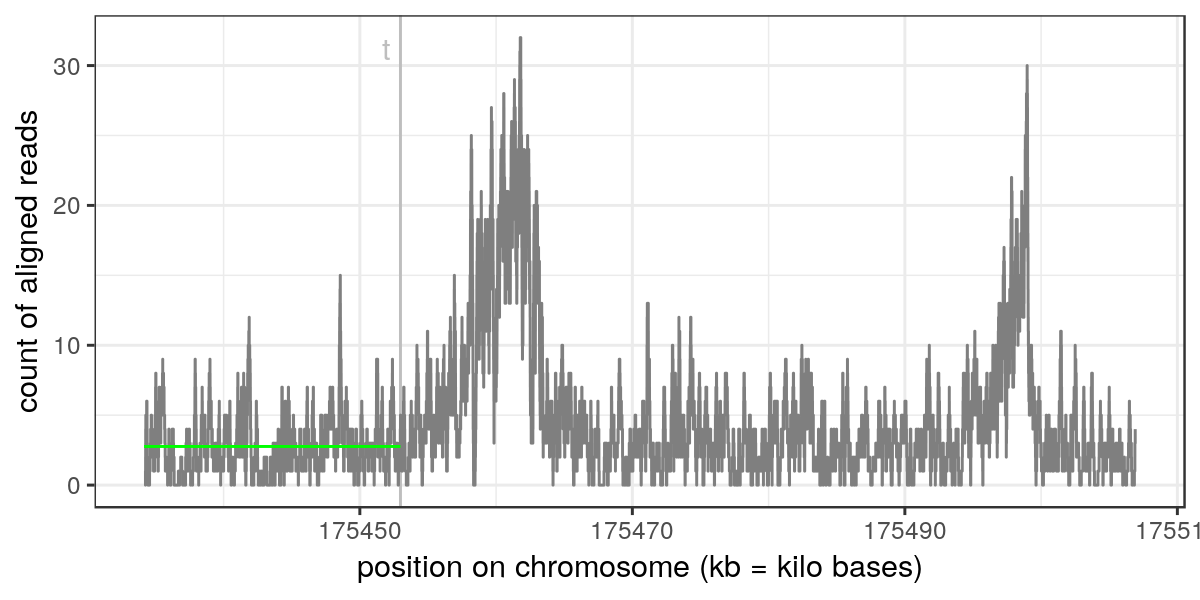
\includegraphics[width=\textwidth]{figure-dp-first-1.png}

$$
\mathcal L_{1, t} =
\underbrace{
  c_{(0, t]}
}_{
  \text{optimal loss of 1st segment $(0, t]$}
}
$$

\end{frame}
 
\begin{frame}
\frametitle{Computation of optimal loss $\mathcal L_{s, t}$
  for $s=1$ segments up to data point $t$}
  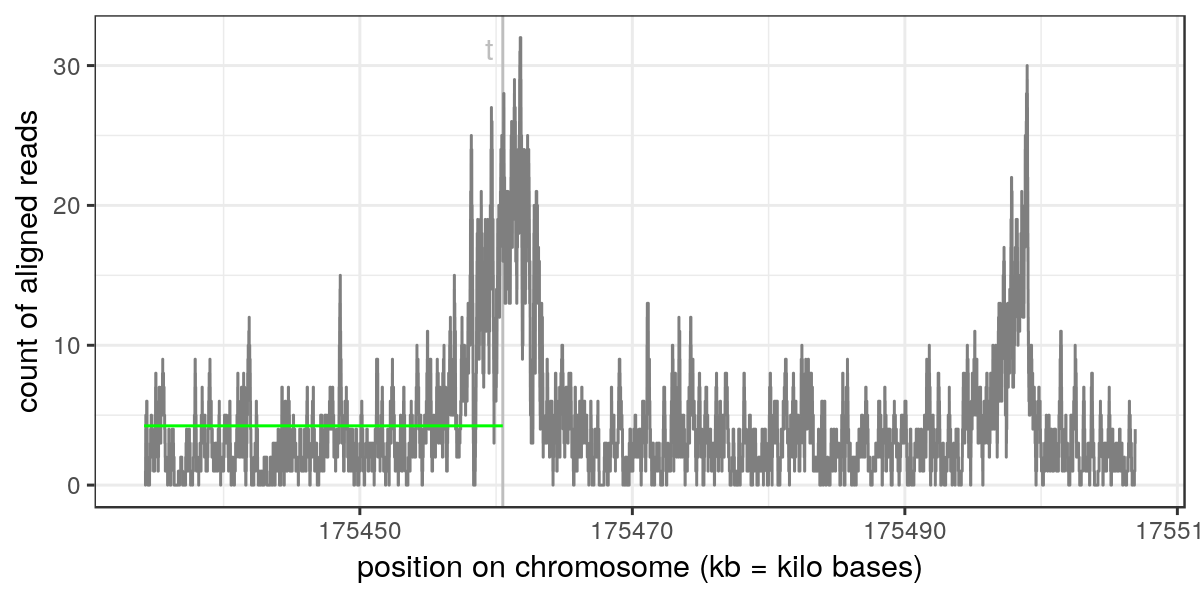
\includegraphics[width=\textwidth]{figure-dp-first-2.png}

$$
\mathcal L_{1, t} =
\underbrace{
  c_{(0, t]}
}_{
  \text{optimal loss of 1st segment $(0, t]$}
}
$$

\end{frame}
 
\begin{frame}
\frametitle{Computation of optimal loss $\mathcal L_{s, t}$
  for $s=1$ segments up to data point $t$}
  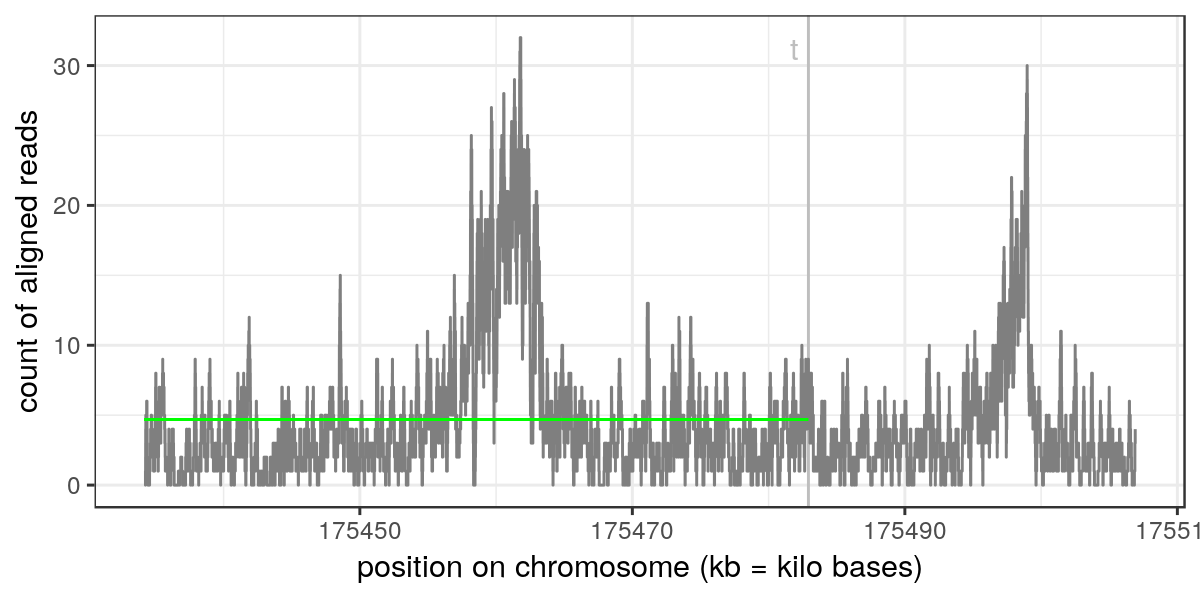
\includegraphics[width=\textwidth]{figure-dp-first-3.png}

$$
\mathcal L_{1, t} =
\underbrace{
  c_{(0, t]}
}_{
  \text{optimal loss of 1st segment $(0, t]$}
}
$$

\end{frame}



\begin{frame}
\frametitle{Computation of optimal loss $\mathcal L_{s, t}$
  for $s=2$ segments up to data point $t < d$}
  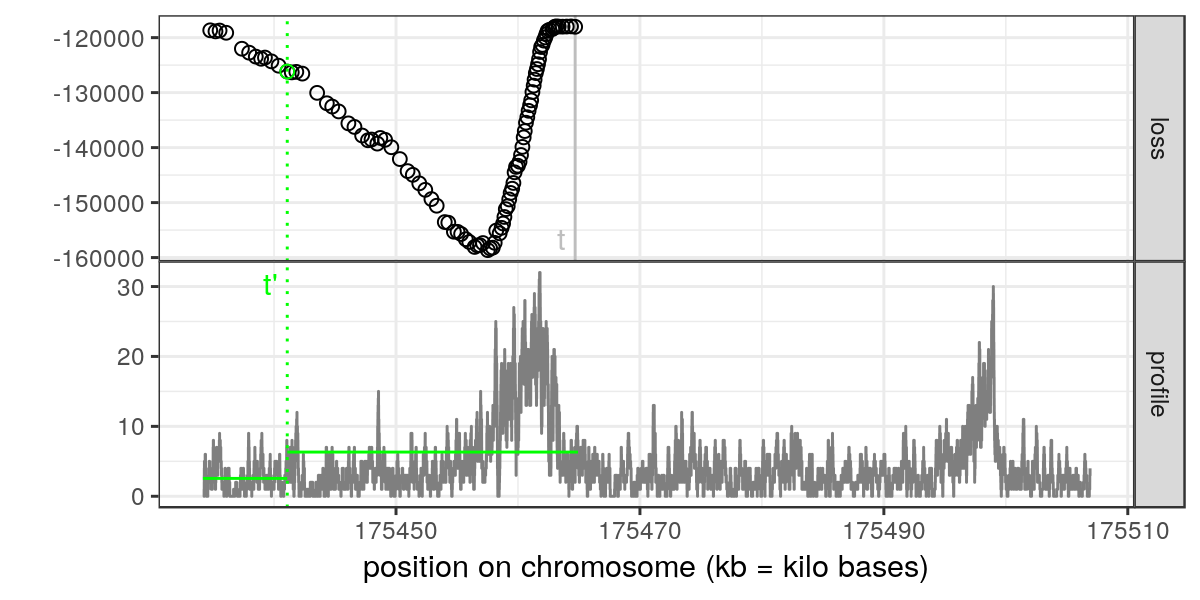
\includegraphics[width=\textwidth]{figure-dp-short-1.png}

$$
\mathcal L_{2, t} =
\min_{
  t' < t
}
\underbrace{
  \mathcal L_{1, t'}
}_{
  \text{optimal loss in 1 segment up to $t'$}
}
+
\underbrace{
  c_{(t', t]}
}_{
  \text{optimal loss of 2nd segment $(t', t]$}
}
$$

\end{frame}
 
\begin{frame}
\frametitle{Computation of optimal loss $\mathcal L_{s, t}$
  for $s=2$ segments up to data point $t < d$}
  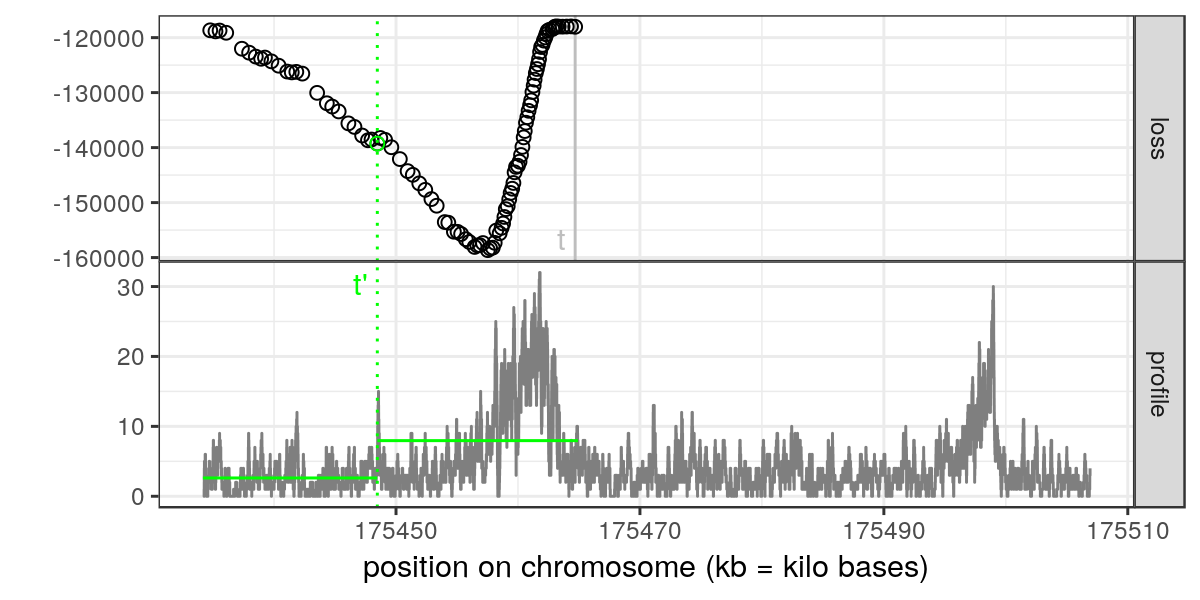
\includegraphics[width=\textwidth]{figure-dp-short-2.png}

$$
\mathcal L_{2, t} =
\min_{
  t' < t
}
\underbrace{
  \mathcal L_{1, t'}
}_{
  \text{optimal loss in 1 segment up to $t'$}
}
+
\underbrace{
  c_{(t', t]}
}_{
  \text{optimal loss of 2nd segment $(t', t]$}
}
$$

\end{frame}
 
\begin{frame}
\frametitle{Computation of optimal loss $\mathcal L_{s, t}$
  for $s=2$ segments up to data point $t < d$}
  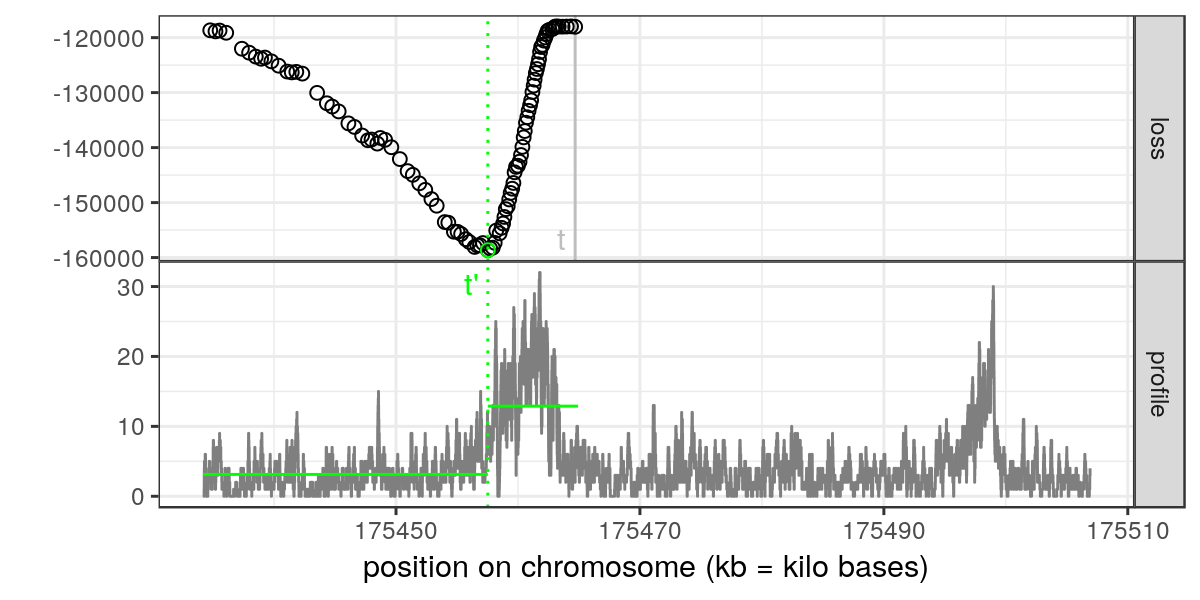
\includegraphics[width=\textwidth]{figure-dp-short-3.png}

$$
\mathcal L_{2, t} =
\min_{
  t' < t
}
\underbrace{
  \mathcal L_{1, t'}
}_{
  \text{optimal loss in 1 segment up to $t'$}
}
+
\underbrace{
  c_{(t', t]}
}_{
  \text{optimal loss of 2nd segment $(t', t]$}
}
$$

\end{frame}
 
\begin{frame}
\frametitle{Computation of optimal loss $\mathcal L_{s, t}$
  for $s=2$ segments up to data point $t < d$}
  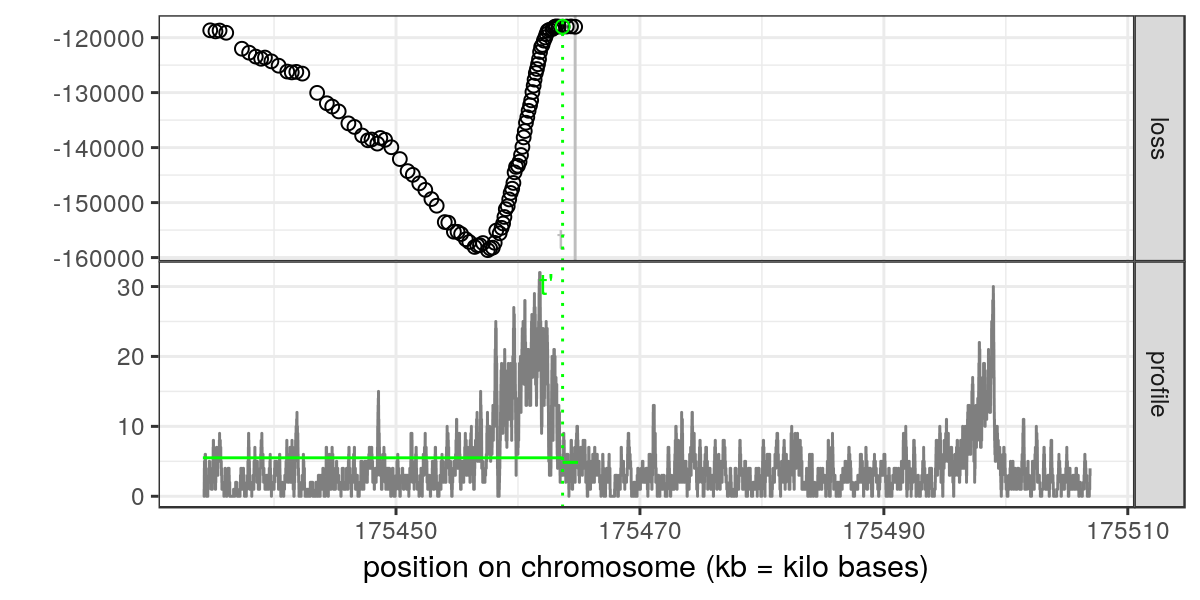
\includegraphics[width=\textwidth]{figure-dp-short-4.png}

$$
\mathcal L_{2, t} =
\min_{
  t' < t
}
\underbrace{
  \mathcal L_{1, t'}
}_{
  \text{optimal loss in 1 segment up to $t'$}
}
+
\underbrace{
  c_{(t', t]}
}_{
  \text{optimal loss of 2nd segment $(t', t]$}
}
$$

\end{frame}



\begin{frame}
\frametitle{Computation of optimal loss $\mathcal L_{s, t}$
 for $s=2$ segments up to last data point $t = d$}
  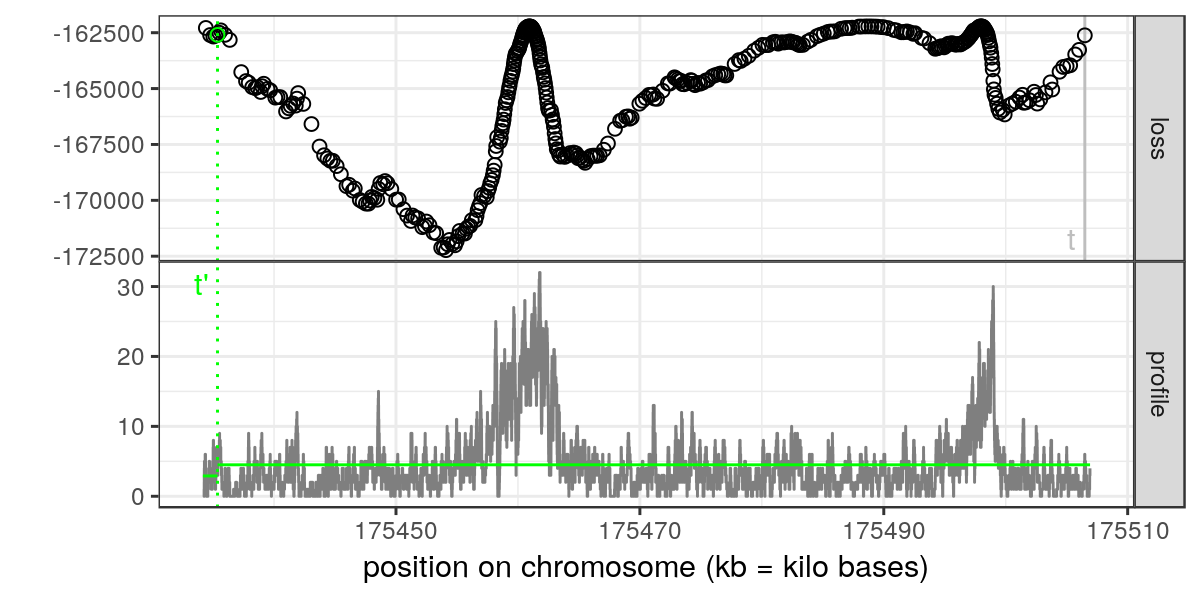
\includegraphics[width=\textwidth]{figure-dp-1.png}

$$
\mathcal L_{2, t} =
\min_{
  t' < t
}
\underbrace{
  \mathcal L_{1, t'}
}_{
  \text{optimal loss in 1 segment up to $t'$}
}
+
\underbrace{
  c_{(t', t]}
}_{
  \text{optimal loss of 2nd segment $(t', t]$}
}
$$

\end{frame}
 
\begin{frame}
\frametitle{Computation of optimal loss $\mathcal L_{s, t}$
 for $s=2$ segments up to last data point $t = d$}
  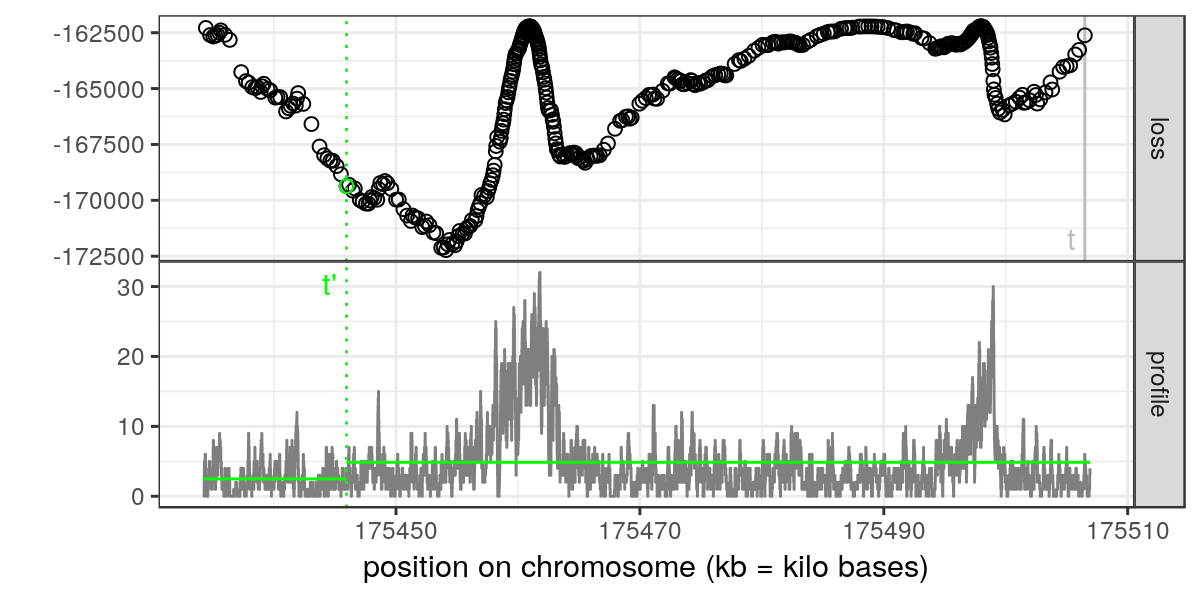
\includegraphics[width=\textwidth]{figure-dp-2.png}

$$
\mathcal L_{2, t} =
\min_{
  t' < t
}
\underbrace{
  \mathcal L_{1, t'}
}_{
  \text{optimal loss in 1 segment up to $t'$}
}
+
\underbrace{
  c_{(t', t]}
}_{
  \text{optimal loss of 2nd segment $(t', t]$}
}
$$

\end{frame}
 
\begin{frame}
\frametitle{Computation of optimal loss $\mathcal L_{s, t}$
 for $s=2$ segments up to last data point $t = d$}
  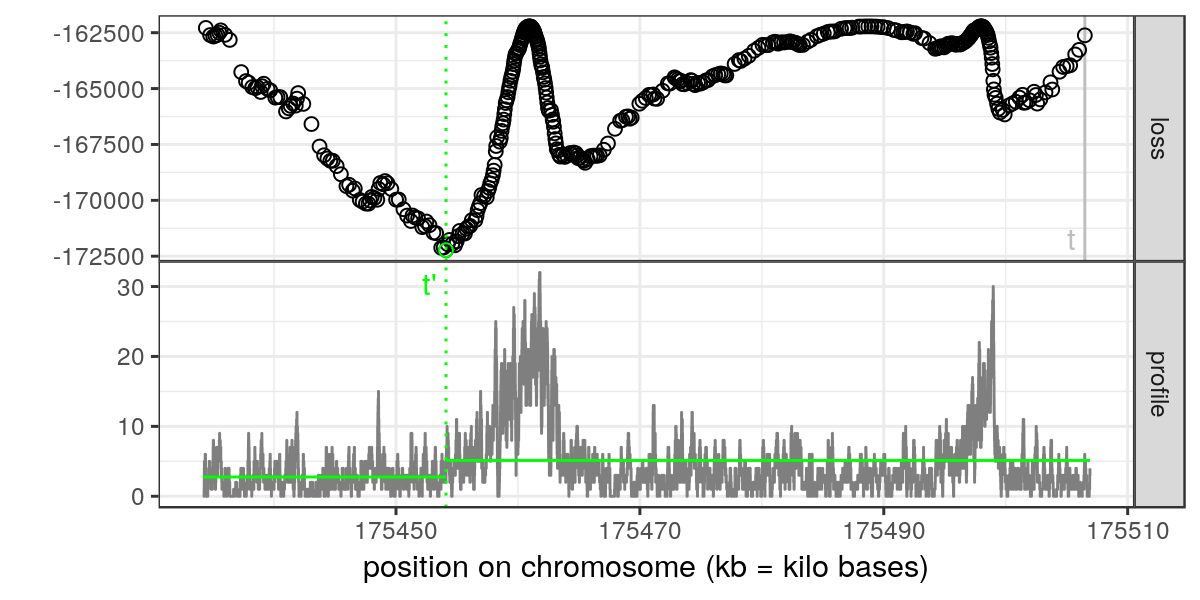
\includegraphics[width=\textwidth]{figure-dp-3.png}

$$
\mathcal L_{2, t} =
\min_{
  t' < t
}
\underbrace{
  \mathcal L_{1, t'}
}_{
  \text{optimal loss in 1 segment up to $t'$}
}
+
\underbrace{
  c_{(t', t]}
}_{
  \text{optimal loss of 2nd segment $(t', t]$}
}
$$

\end{frame}
 
\begin{frame}
\frametitle{Computation of optimal loss $\mathcal L_{s, t}$
 for $s=2$ segments up to last data point $t = d$}
  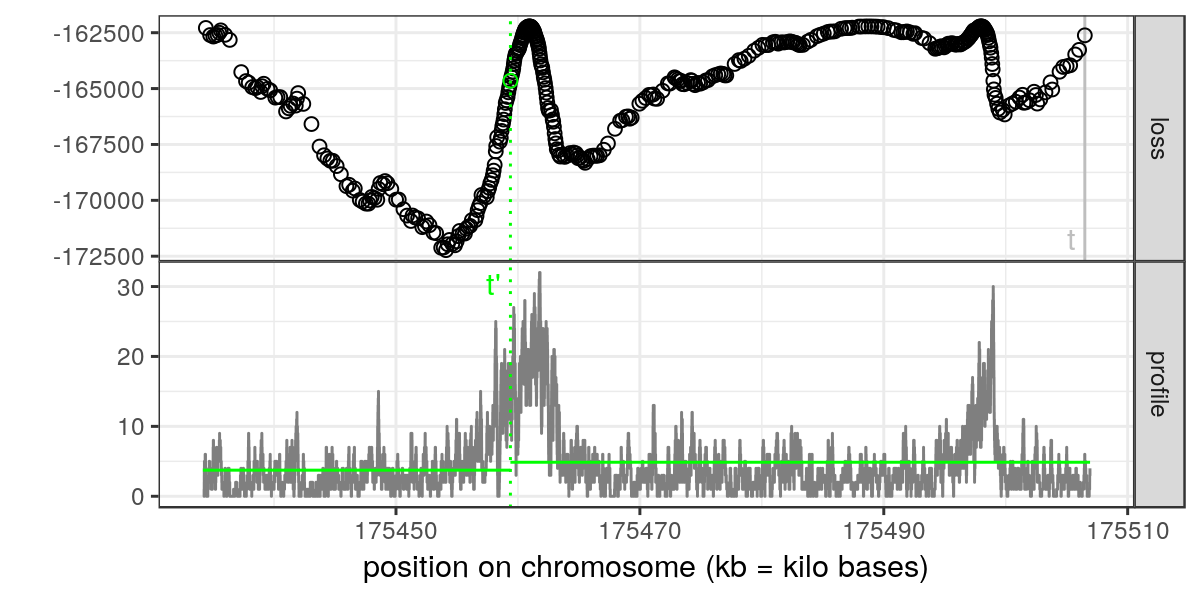
\includegraphics[width=\textwidth]{figure-dp-4.png}

$$
\mathcal L_{2, t} =
\min_{
  t' < t
}
\underbrace{
  \mathcal L_{1, t'}
}_{
  \text{optimal loss in 1 segment up to $t'$}
}
+
\underbrace{
  c_{(t', t]}
}_{
  \text{optimal loss of 2nd segment $(t', t]$}
}
$$

\end{frame}
 
\begin{frame}
\frametitle{Computation of optimal loss $\mathcal L_{s, t}$
 for $s=2$ segments up to last data point $t = d$}
  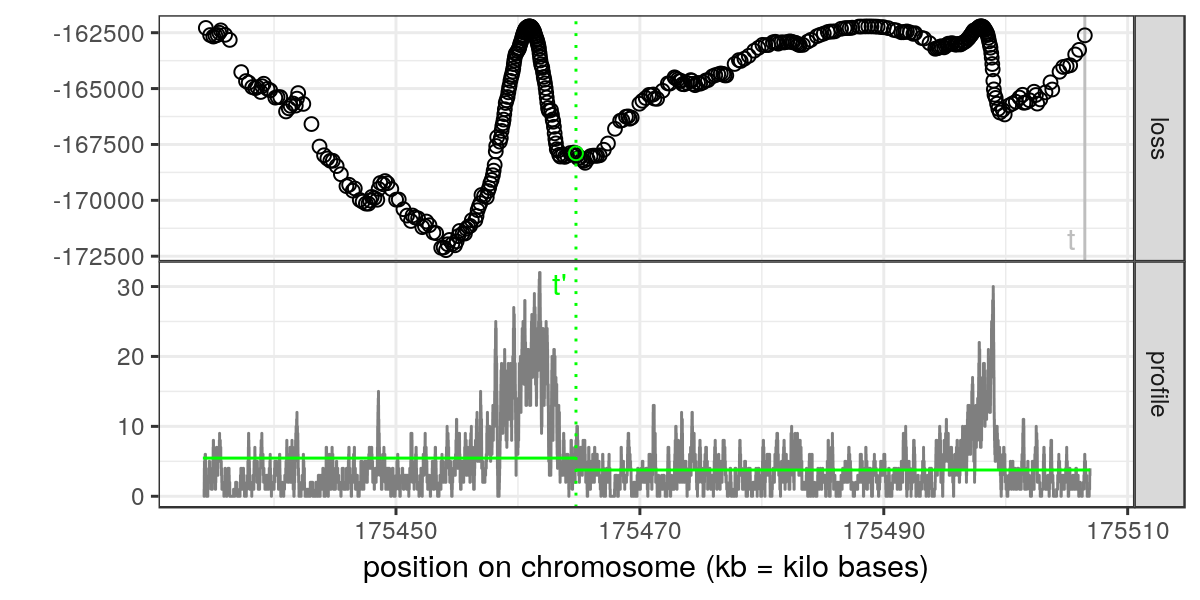
\includegraphics[width=\textwidth]{figure-dp-5.png}

$$
\mathcal L_{2, t} =
\min_{
  t' < t
}
\underbrace{
  \mathcal L_{1, t'}
}_{
  \text{optimal loss in 1 segment up to $t'$}
}
+
\underbrace{
  c_{(t', t]}
}_{
  \text{optimal loss of 2nd segment $(t', t]$}
}
$$

\end{frame}
 
\begin{frame}
\frametitle{Computation of optimal loss $\mathcal L_{s, t}$
 for $s=2$ segments up to last data point $t = d$}
  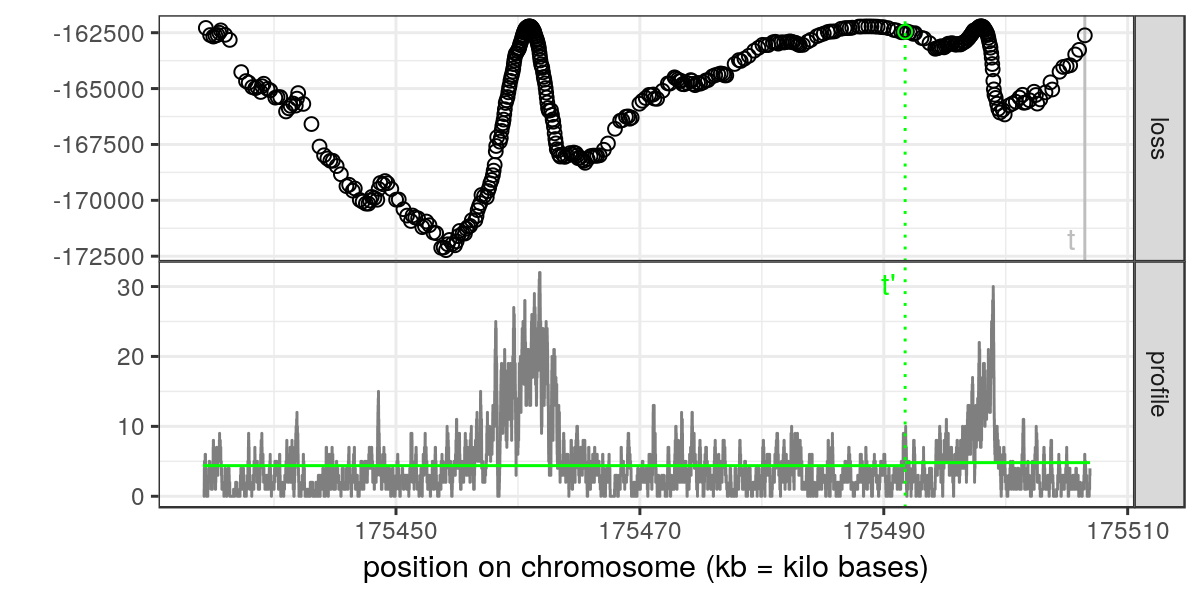
\includegraphics[width=\textwidth]{figure-dp-6.png}

$$
\mathcal L_{2, t} =
\min_{
  t' < t
}
\underbrace{
  \mathcal L_{1, t'}
}_{
  \text{optimal loss in 1 segment up to $t'$}
}
+
\underbrace{
  c_{(t', t]}
}_{
  \text{optimal loss of 2nd segment $(t', t]$}
}
$$

\end{frame}


\begin{frame}
  \frametitle{Dynamic programming is faster than grid search for $s>
    2$ segments}

  Computation time in number of data points $n$:

  \vskip 1cm

  \begin{tabular}{ccc}
    segments $s$ & grid search & dynamic programming \\
    \hline
    1 & $O(n)$ & $O(n)$ \\
    2 & $O(n^2)$ & $O(n^2)$ \\
    3 & $O(n^3)$ & $O(n^2)$ \\
    4 & $O(n^4)$ & $O(n^2)$ \\
    $\vdots$ &     $\vdots$ &     $\vdots$ 
  \end{tabular}

  \vskip 1cm

  For example $n = 5735$ data points to segment.\\
  $n^2 = 32890225$\\
  $n^3 = 188625440375$\\
  $\vdots$
\end{frame}


\begin{frame}
\frametitle{Computation of optimal loss $\mathcal L_{s, t}$
 for $s=3$ segments up to data point $t$}
  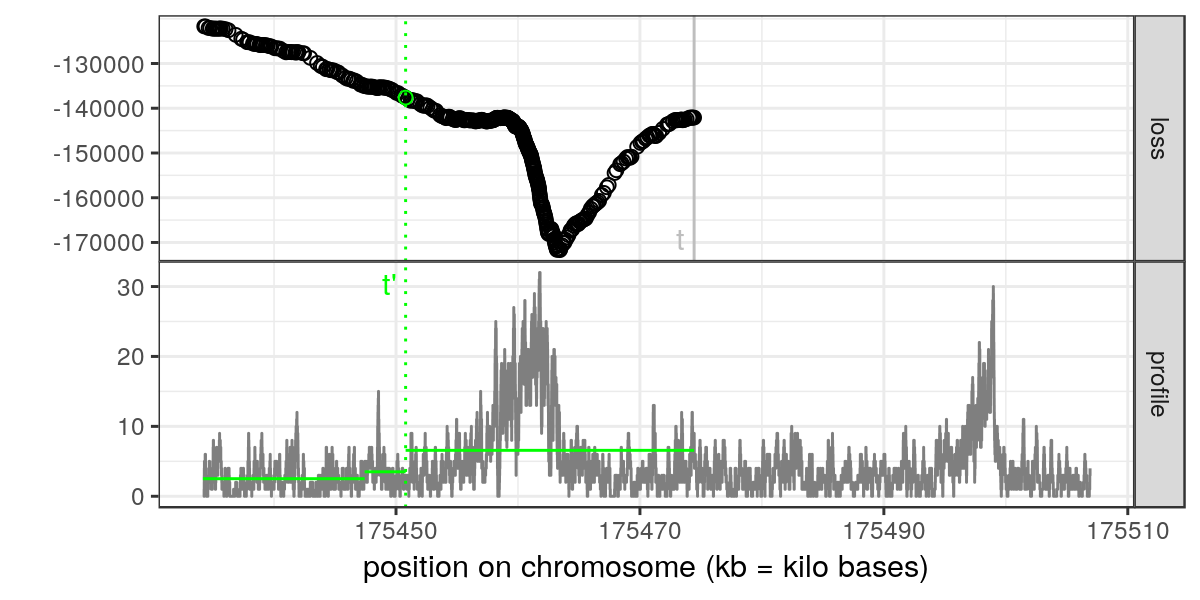
\includegraphics[width=\textwidth]{figure-dp-third-1.png}

$$
\mathcal L_{3, t} =
\min_{
  t' < t
}
\underbrace{
  \mathcal L_{2, t'}
}_{
  \text{optimal loss in 2 segments up to $t'$}
}
+
\underbrace{
  c_{(t', t]}
}_{
  \text{optimal loss of 3rd segment $(t', t]$}
}
$$

\end{frame}
 
\begin{frame}
\frametitle{Computation of optimal loss $\mathcal L_{s, t}$
 for $s=3$ segments up to data point $t$}
  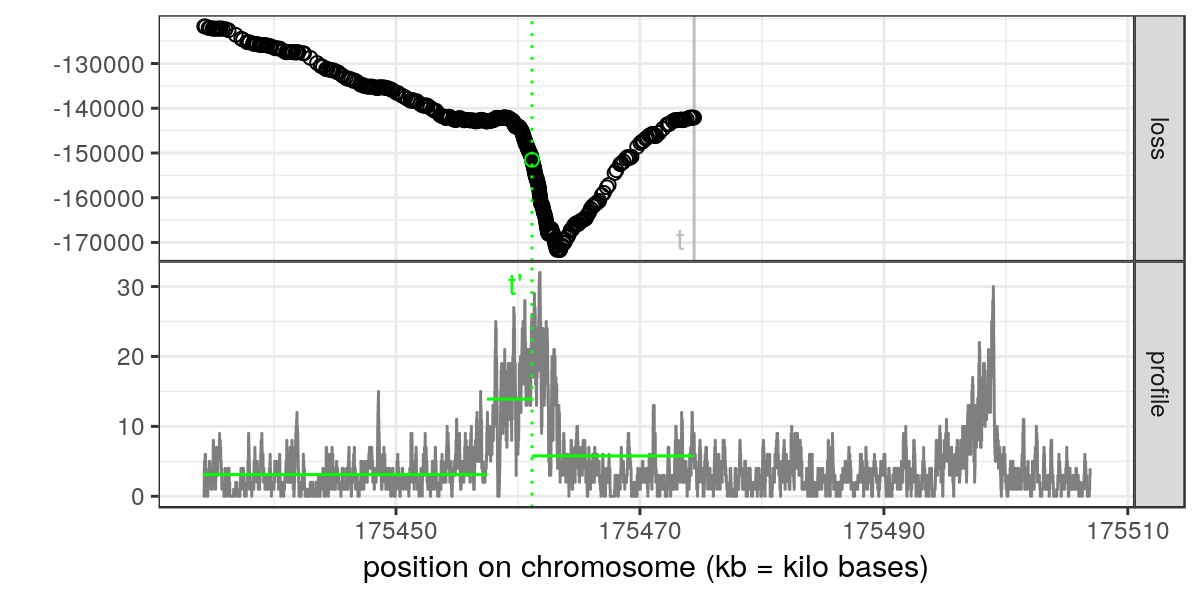
\includegraphics[width=\textwidth]{figure-dp-third-2.png}

$$
\mathcal L_{3, t} =
\min_{
  t' < t
}
\underbrace{
  \mathcal L_{2, t'}
}_{
  \text{optimal loss in 2 segments up to $t'$}
}
+
\underbrace{
  c_{(t', t]}
}_{
  \text{optimal loss of 3rd segment $(t', t]$}
}
$$

\end{frame}
 
\begin{frame}
\frametitle{Computation of optimal loss $\mathcal L_{s, t}$
 for $s=3$ segments up to data point $t$}
  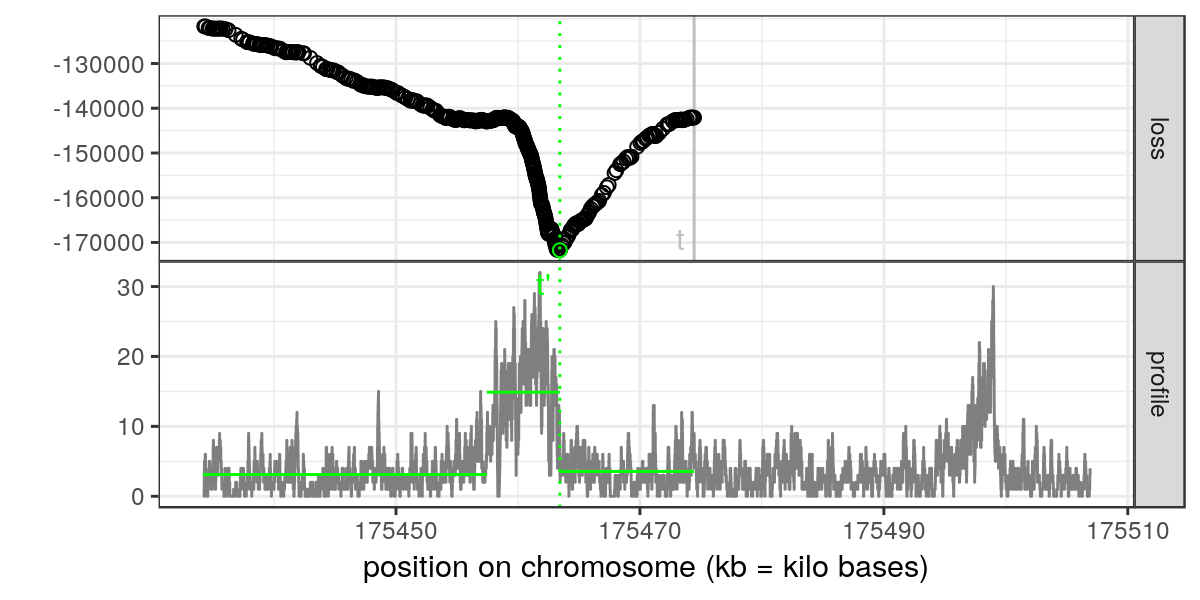
\includegraphics[width=\textwidth]{figure-dp-third-3.png}

$$
\mathcal L_{3, t} =
\min_{
  t' < t
}
\underbrace{
  \mathcal L_{2, t'}
}_{
  \text{optimal loss in 2 segments up to $t'$}
}
+
\underbrace{
  c_{(t', t]}
}_{
  \text{optimal loss of 3rd segment $(t', t]$}
}
$$

\end{frame}
 
\begin{frame}
\frametitle{Computation of optimal loss $\mathcal L_{s, t}$
 for $s=3$ segments up to data point $t$}
  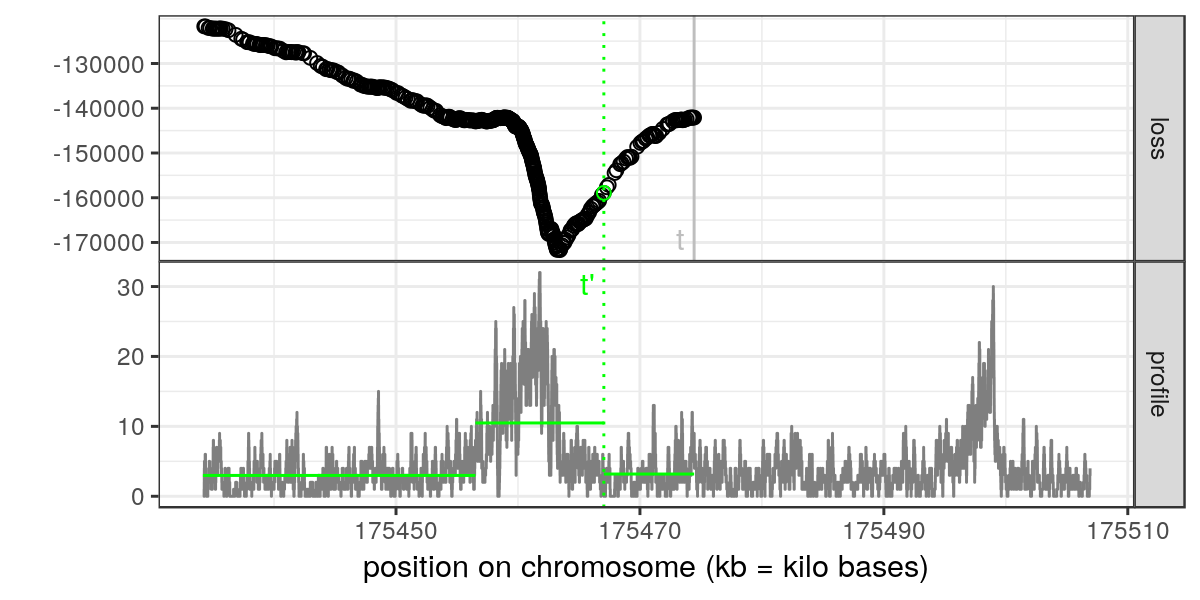
\includegraphics[width=\textwidth]{figure-dp-third-4.png}

$$
\mathcal L_{3, t} =
\min_{
  t' < t
}
\underbrace{
  \mathcal L_{2, t'}
}_{
  \text{optimal loss in 2 segments up to $t'$}
}
+
\underbrace{
  c_{(t', t]}
}_{
  \text{optimal loss of 3rd segment $(t', t]$}
}
$$

\end{frame}


\section{Functional pruning algorithms}

\begin{frame}
  \frametitle{Classical dynamic programming is too slow for big data}
  \begin{itemize}
  \item Motivated by big data sequences $n>1000$ in genomics and other
    fields, for which $O(n^2)$ is too slow.
  \item Recent work into functional pruning algorithms which compute
    the same solution in $O(n\log n)$ (empirically).
  \item Independent discovery by Rigaill arXiv:1004.0887, JFdS 2015;
    Johnson PhD 2011, JCGS 2013. Main idea: first minimize on the last
    changepoint $t_{S-1}$, then on the last segment mean $u_S$:
  \end{itemize}
\begin{eqnarray*}
  \mathcal L_{S,n} &=& \min_{t_{S-1}}
\mathcal L_{S-1, t_{S-1}}
 +
\underbrace{\alert{\min_{u_S}} \sum_{i=t_{S-1}+1}^{t_S=n} \ell( u_S,  z_i)}_{
c_{(t_{S-1}, t_S=n]}
}\text{ --- classical}\\
&=& \alert{\min_{u_S} }
\underbrace{
\min_{t_{S-1}}
\mathcal L_{S-1, t_{S-1}}
 +
\sum_{i=t_{S-1}+1}^{t_S=n} \ell( u_S,  z_i)
}_{
C_{S,n}(u_S)
}\text{ --- functional}
\end{eqnarray*}
\end{frame}

\begin{frame}
  \frametitle{Functional cost representation results in pruning}
  
  Maidstone, {\it et al.} Statistics and Computing 2016.
\centering
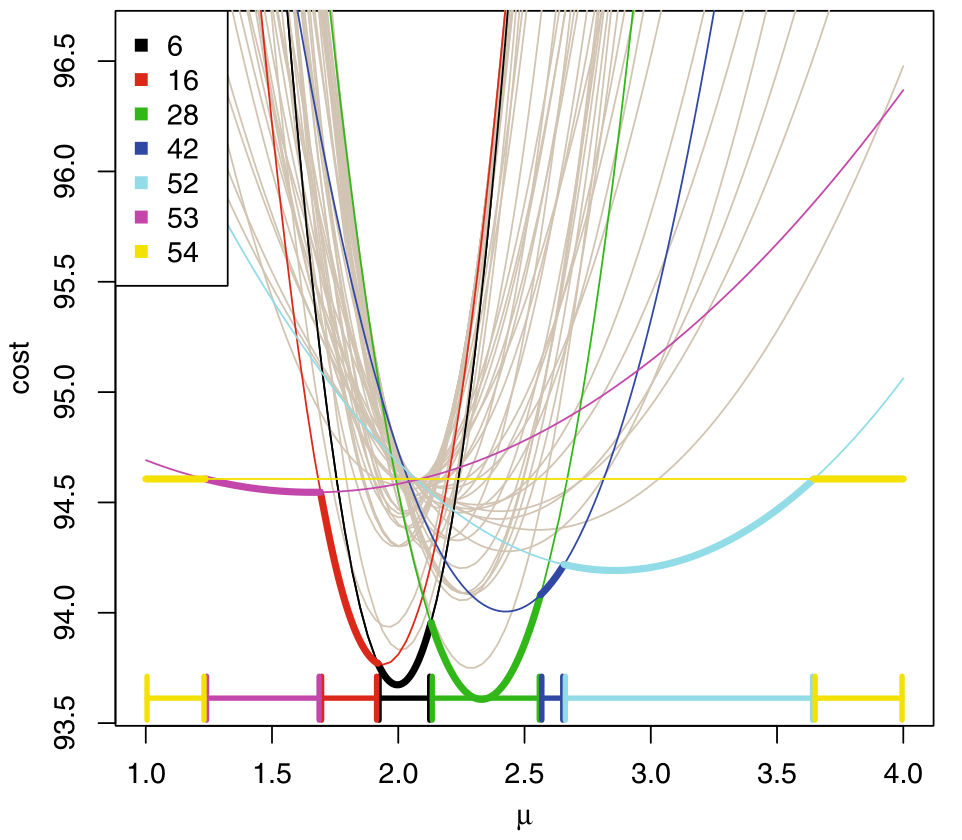
\includegraphics[width=0.7\textwidth]{screenshot-Maidstone-figure-1}

\begin{itemize}
\item Only need to store the minimum cost (colored lines/intervals).
  \item No need to consider the cost functions/changepoints which are
    not optimal for any mean values (grey lines).
\end{itemize}
  
\end{frame}

\section{Empirical time complexity}

\begin{frame}
  \frametitle{Number of intervals in real and simulated data}
  Rigaill, arXiv:1004.0887.

  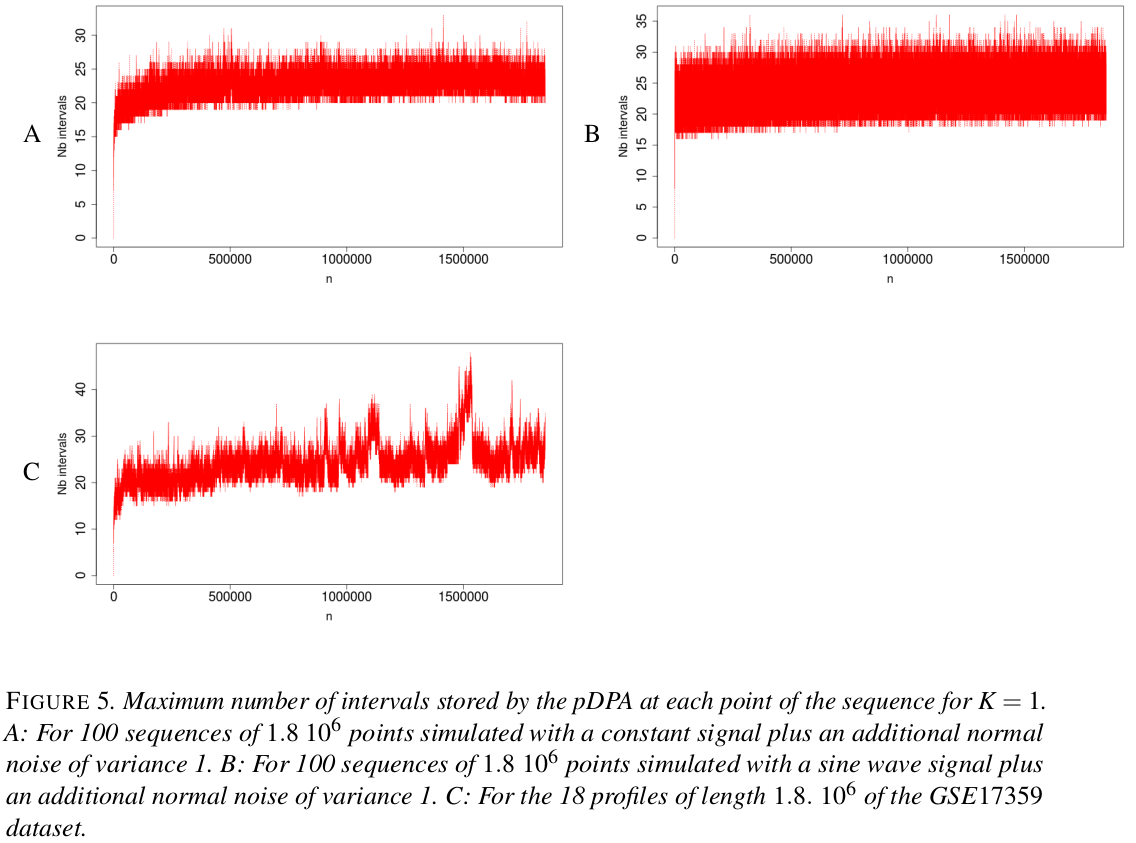
\includegraphics[width=\textwidth]{screenshot-figure-5}
\end{frame}

\begin{frame}
  \frametitle{Another fast functional pruning algorithm}
  Maidstone, {\it et al.} Statistics and Computing 2016.
\vskip -0.5cm
\begin{align*}
    \minimize_{\substack{
  \mathbf m\in\RR^{n}
  }} &\ \ 
    \sum_{i=1}^n \ell( m_i,  z_i)  + \lambda{\sum_{i=1}^{n-1}I[m_{i}\neq m_{i+1}]}
  \nonumber 
\end{align*}

\centering
  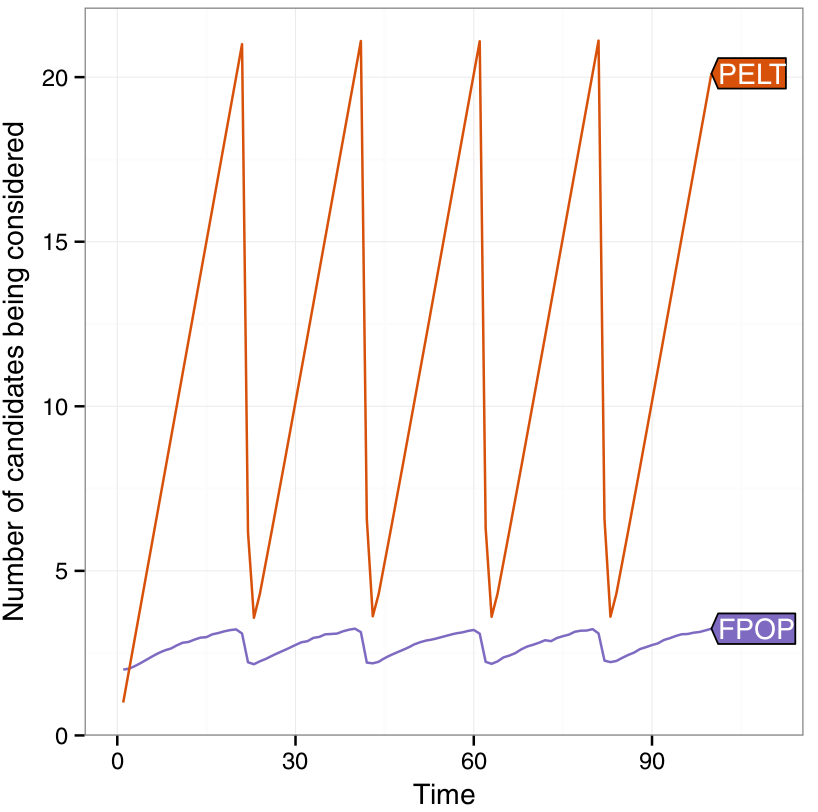
\includegraphics[width=0.48\textwidth]{screenshot-Maidstone-figure-4}
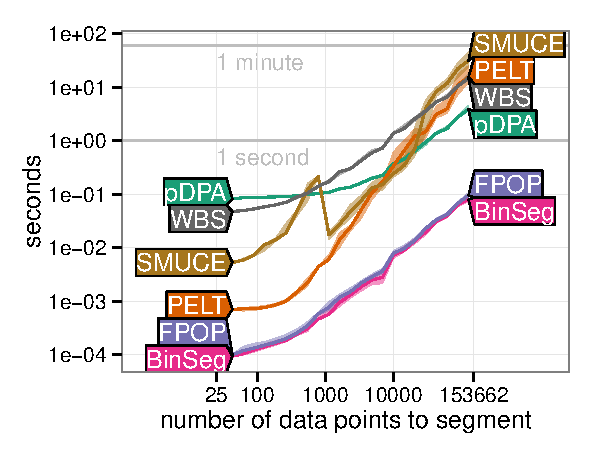
\includegraphics[width=0.48\textwidth]{figure-systemtime-arrays-bins}
  
\end{frame}

\begin{frame}
  \frametitle{Algorithm with constraints is also fast}
  H, {\it et al.} Journal of Machine Learning Research 21(87):1--40, 2020. 
\vskip -0.5cm
  \begin{align*}
    \minimize_{\substack{
  \mathbf m\in\RR^{n}
  }} &\ \ 
    \sum_{i=1}^n \ell( m_i,  z_i) 
\\
      \text{subject to} &\ \ {{\sum_{i=1}^{n-1} I[m_i\neq m_{i+1}]}=S-1,}
  \nonumber\\
  &\ \ \text{...up-down constraints on $m$.}
  \nonumber 
\end{align*}

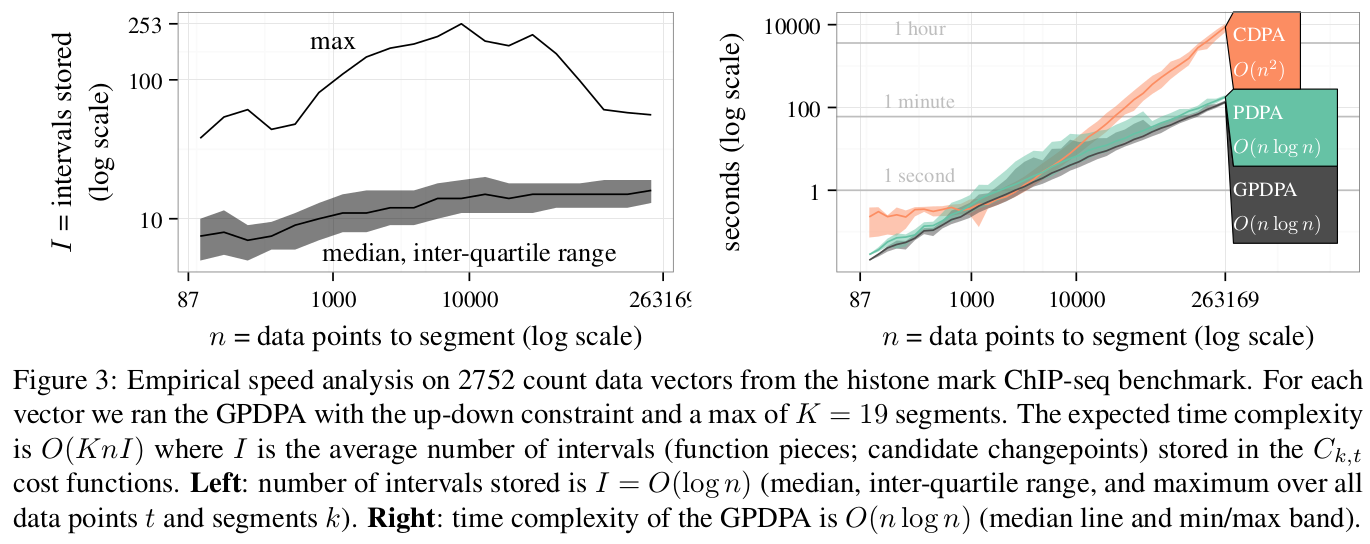
\includegraphics[width=\textwidth]{screenshot-GPDPA-intervals}

\end{frame}


\begin{frame}
  \frametitle{Another fast constrained algorithm for neuroscience}
  Jewell, {\it et al.} {\it Biostatistics} 2019.
\vskip -0.5cm
\begin{align*}
    \minimize_{c_1,\dots,c_T, z_2, \dots, z_T} &\ \ 
    \frac 1 2 \sum_{t=1}^T (y_t-c_t)^2  + 
\lambda\sum_{t=2}^{T} 1_{(z_t\neq 0)}
\\
      \text{subject to} &\ \ z_t = c_t - \gamma c_{t-1} \geq 0.
  \nonumber 
\end{align*}

\centering

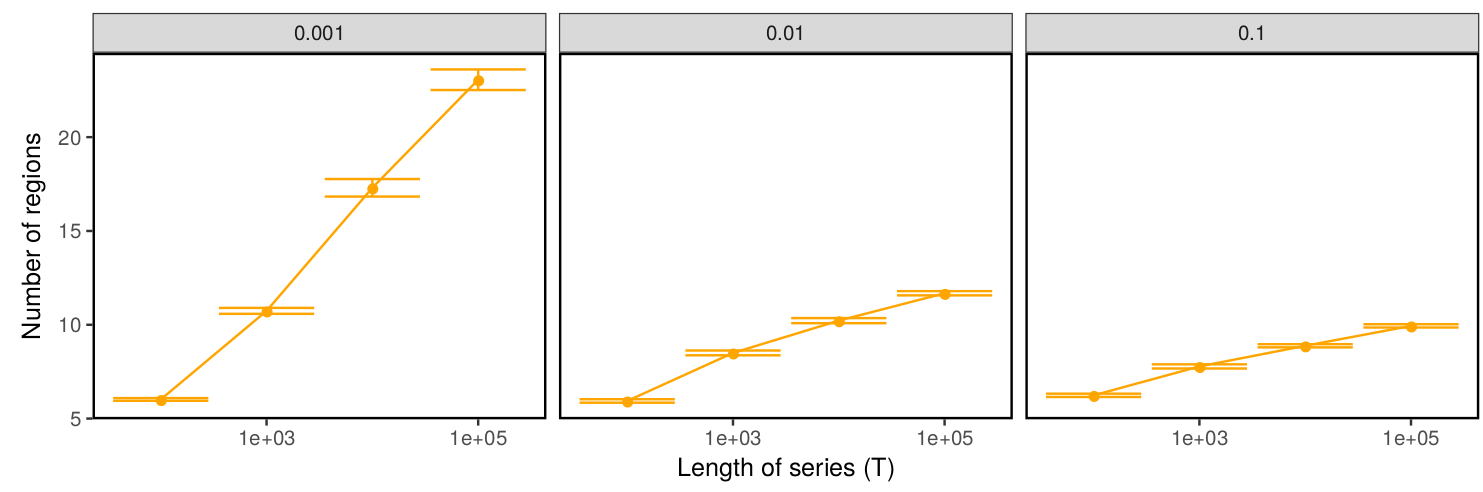
\includegraphics[width=0.8\textwidth]{screenshot-jewell-intervals}

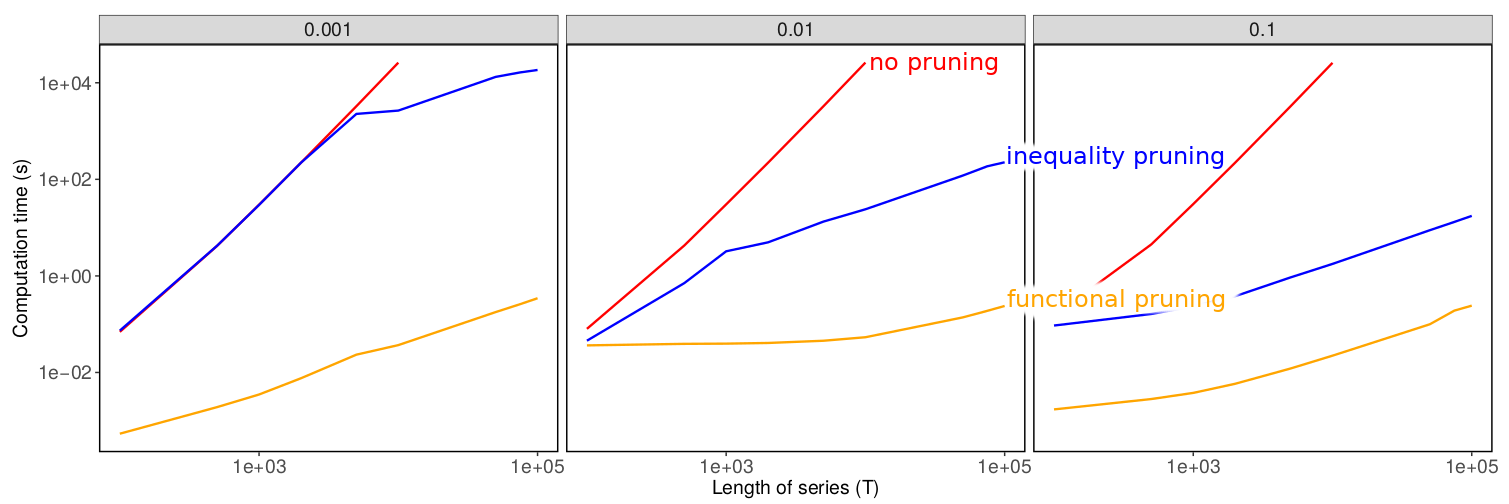
\includegraphics[width=0.8\textwidth]{screenshot-jewell-timings-labels}
  
\end{frame}

\begin{frame}[fragile]
  \frametitle{Another fast constrained algorithm for genomics}

  H, {\it et al.} arXiv:1810.00117, accepted in \emph{J.
    Statistical Software}.
\vskip -0.5cm
\begin{align*}
    \minimize_{\substack{
  \mathbf m\in\RR^{n}
% \\
%    0=t_0<t_1<\cdots<t_{S-1}<t_S=n
  }} &\ \ 
    \sum_{i=1}^n \ell( m_i,  z_i)  + \lambda{\sum_{i=1}^{n-1}I[m_{i}\neq m_{i+1}]}
\\
      \text{subject to} &\ \ \text{...up-down constraints on $m$.}
  \nonumber 
\end{align*}

  \begin{minipage}{0.48\textwidth}
    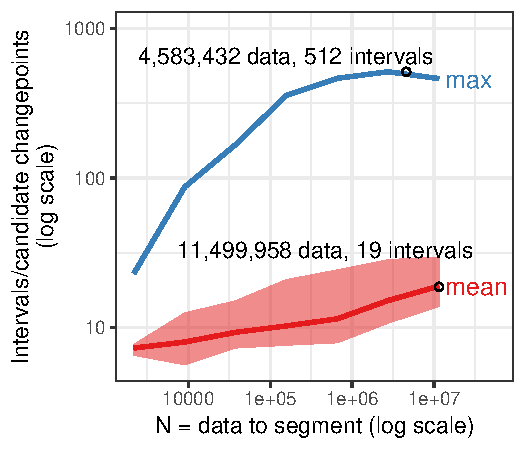
\includegraphics[width=\textwidth]{jss-figure-target-intervals-models}
    $I=O(\log n)$ intervals.
  \end{minipage}
  \begin{minipage}{0.48\textwidth}
    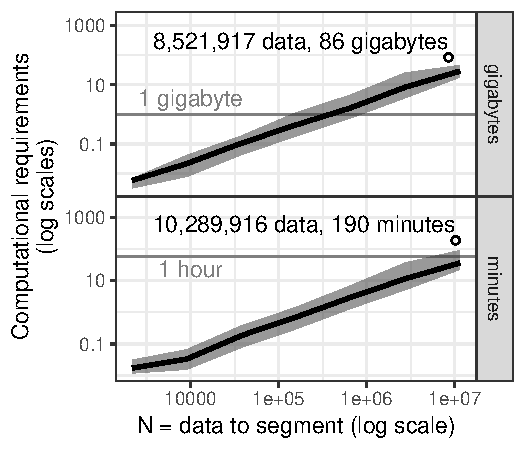
\includegraphics[width=\textwidth]{jss-figure-target-intervals-models-computation}
    Overall  $O(n \log n)$ complexity.
  \end{minipage}
  
\end{frame}

\begin{frame}
\frametitle{Worst case quadratic complexity only observed with synthetic
  data and large penalties}

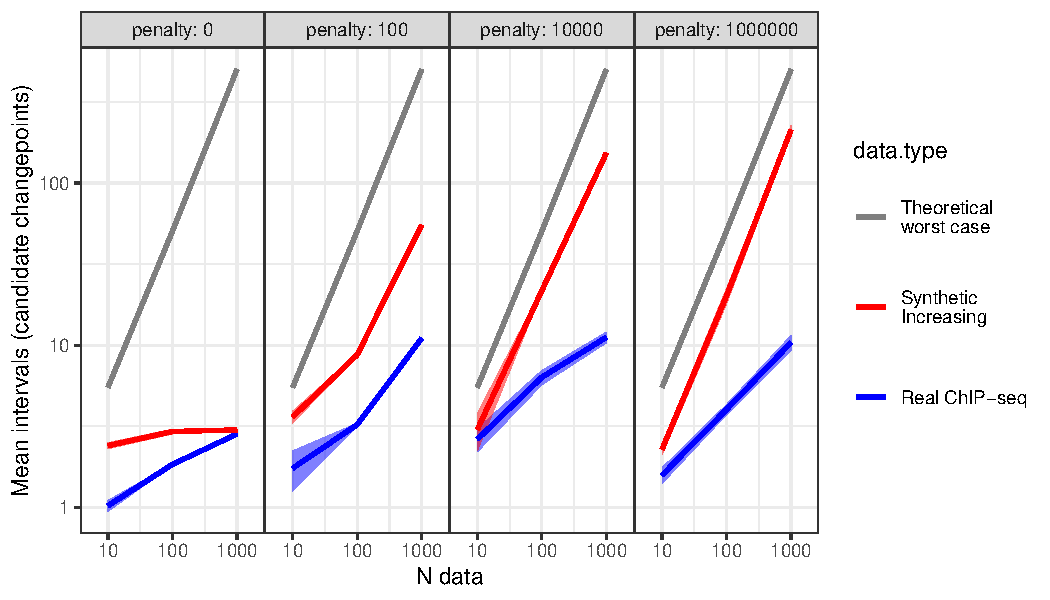
\includegraphics[width=\textwidth]{figure-worst-case}

Mean $\pm$ standard deviation over 10 data sets.

\end{frame}

\section{Theoretical time complexity}

\begin{frame}
  \frametitle{Worst case complexity is quadratic}
  Rigaill, arXiv:1004.0887.
  
  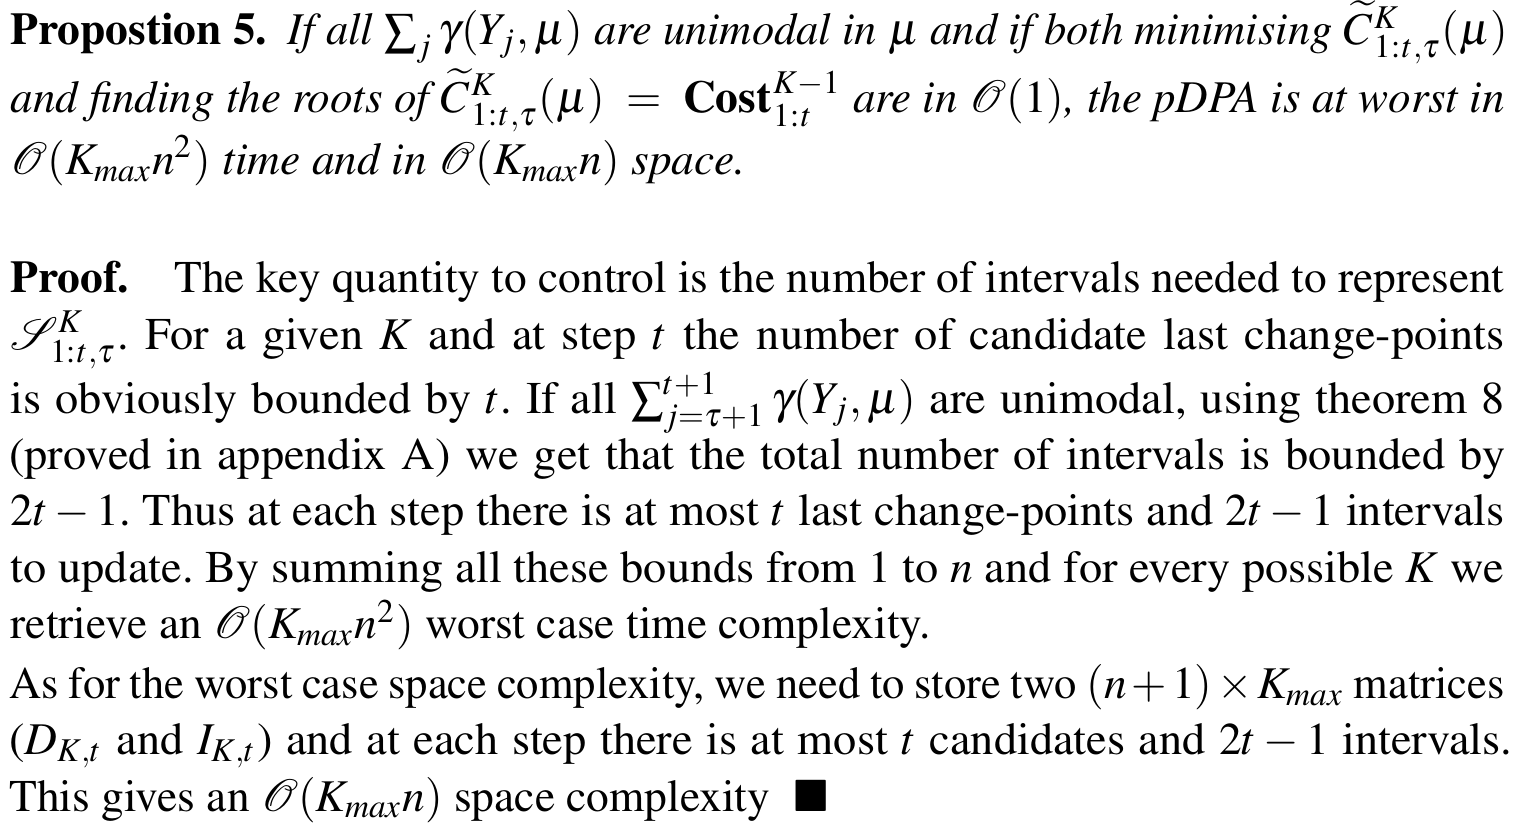
\includegraphics[width=\textwidth]{screenshot-proposition-5}
\end{frame}

\begin{frame}
  \frametitle{Average case complexity proof for uniform loss}
  Rigaill, arXiv:1004.0887.
  
  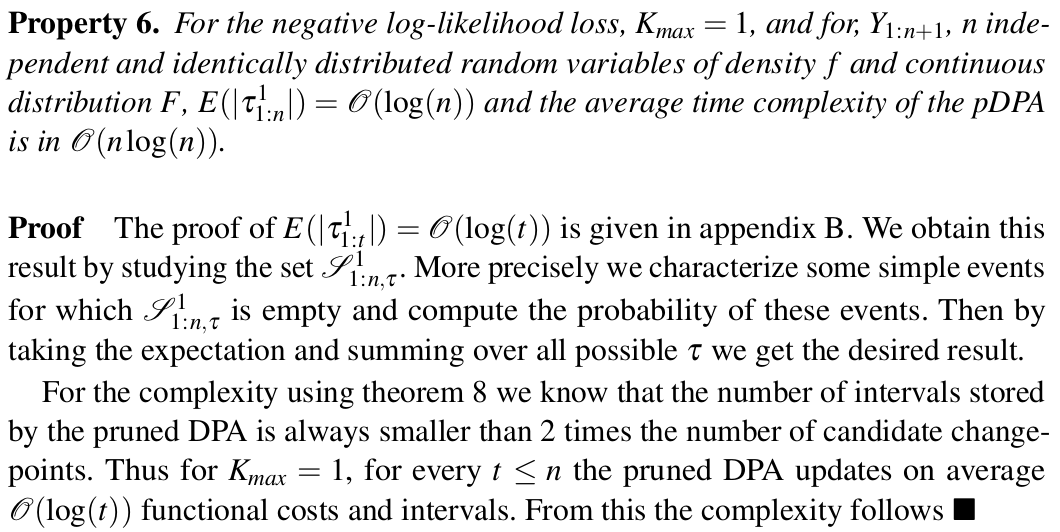
\includegraphics[width=\textwidth]{screenshot-proposition-6}
\end{frame} 

\begin{frame}[fragile]
  \frametitle{Conclusions}

  \begin{itemize}
  \item Optimal detection of $S-1$ changepoints in $n$ data is naively
    a $O(n^S)$ computation.  
  \item Functional pruning method yields algorithms with worst case
    time complexity of $O(n^2)$ (same as classical dynamic
    programming).
  \item Empirically the functional pruning algorithms are much faster,
    $O(n\log n)$.
  \item Only one proof of average time complexity for 1 changepoint
    and the uniform loss function (never used in practice).
  \item Would be interesting to prove $O(n\log n)$ average time complexity in
    other more realistic situations. (square/Poisson loss, $\lambda$) How?
  \item Let's collaborate! toby.hocking@nau.edu
  \end{itemize}
  
\end{frame}

\begin{frame}
  \frametitle{Dynamic programming recursion with functional pruning}
  \begin{itemize}
  \item $\tau$ is first data point on last segment.
  \item $\mu$ is last segment mean.
  \end{itemize}
  \begin{eqnarray*}
    C_{S,n}(\mu) &=&
    \min_{\tau\in\{S, \dots, n\} }
\mathcal L_{S-1, \tau-1}
 +
\sum_{i=\tau}^{n} \ell( \mu,  z_i)\\
&=&\min\{\mathcal L_{S-1,S-1} + \sum_{i=S}^{n} \ell( \mu,  z_i), \dots,\\
    &&\hskip 0.8cm \mathcal L_{S-1,n-1} + \ell( \mu,  z_n) \}\\
&=&\ell( \mu,  z_n) + \min\{\mathcal L_{S-1,S-1} + \sum_{i=S}^{n-1} \ell( \mu,  z_i), \dots,\\
    &&\hskip 2.7cm \mathcal L_{S-1,n-2}  +\ell( \mu,  z_{n-1})\}\\
    &&\hskip 2.7cm \mathcal L_{S-1,n-1}  \}\\
&=&\ell( \mu,  z_n)+
\min\{
    C_{S,n-1}(\mu),\,  
    \mathcal L_{S-1,n-1}
\}
  \end{eqnarray*}
\end{frame}


\begin{frame}
  \frametitle{Example data set with $n=4$}
  Rigaill, arXiv:1004.0887.

  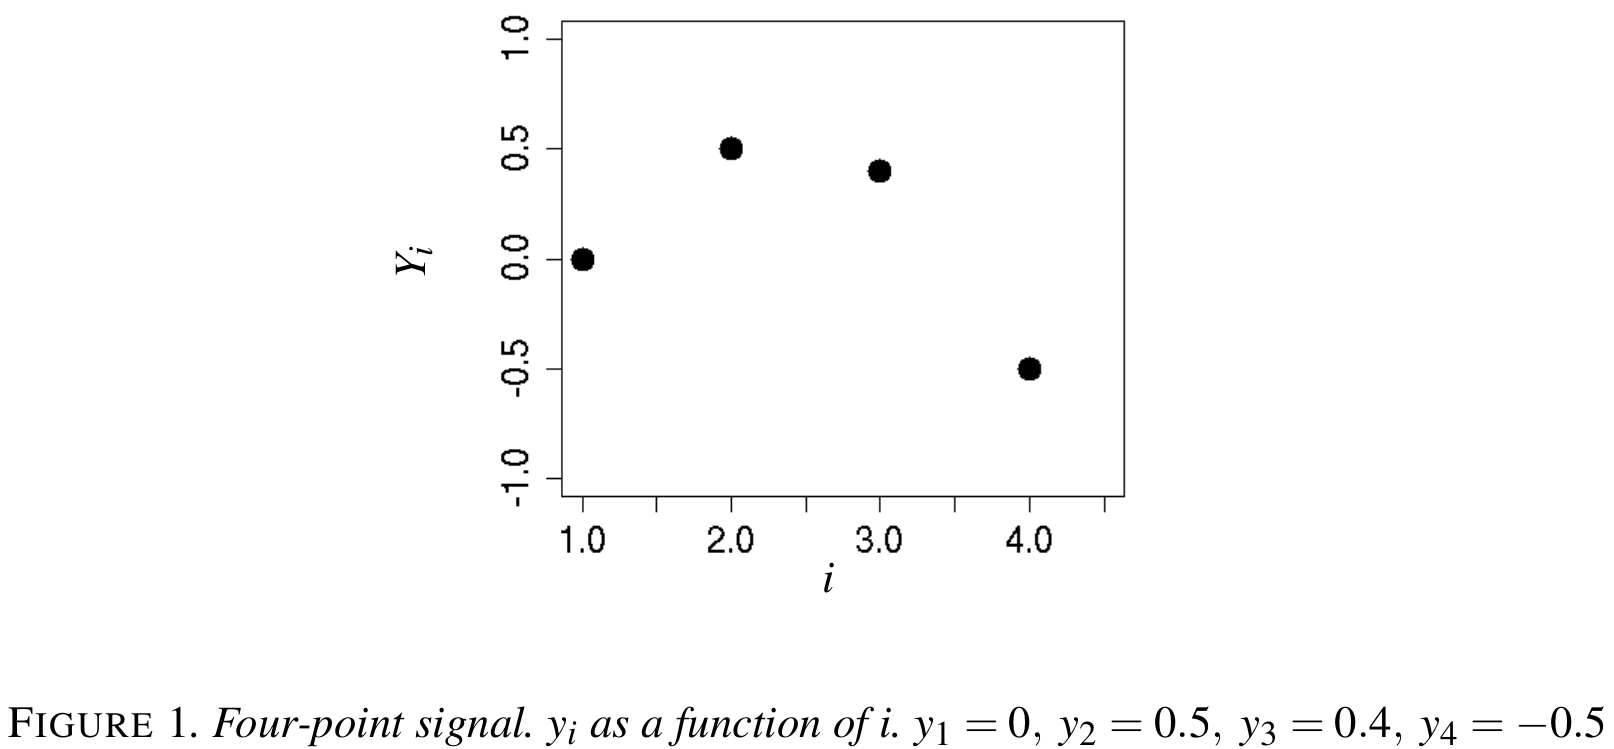
\includegraphics[width=\textwidth]{screenshot-figure-1}
\end{frame}

\begin{frame}
  \frametitle{Functional cost computation at $t=3$}
  Rigaill, arXiv:1004.0887.

  \begin{itemize}
  \item Data: 0, 0.5, 0.4, -0.5. 
  \item $\mathcal L_{1,1}=\min_\mu (\mu-0)^2=0$.
  \item $\mathcal L_{1,2}=\min_\mu (\mu-0)^2 + (\mu-0.5)^2=0.125$.
  \item Computing
    $C_{2,3}(\mu) = \ell(\mu, z_3) + \min\{C_{2,2}(\mu),\, \mathcal
    L_{1,2}\}$:
  \item Change before $\tau=2$: $C_{2,2}(\mu)=\mathcal L_{1,1} + (\mu-0.5)^2$.
  \item Change before $\tau=3$: $\mathcal L_{1,2}$.
  \end{itemize}

  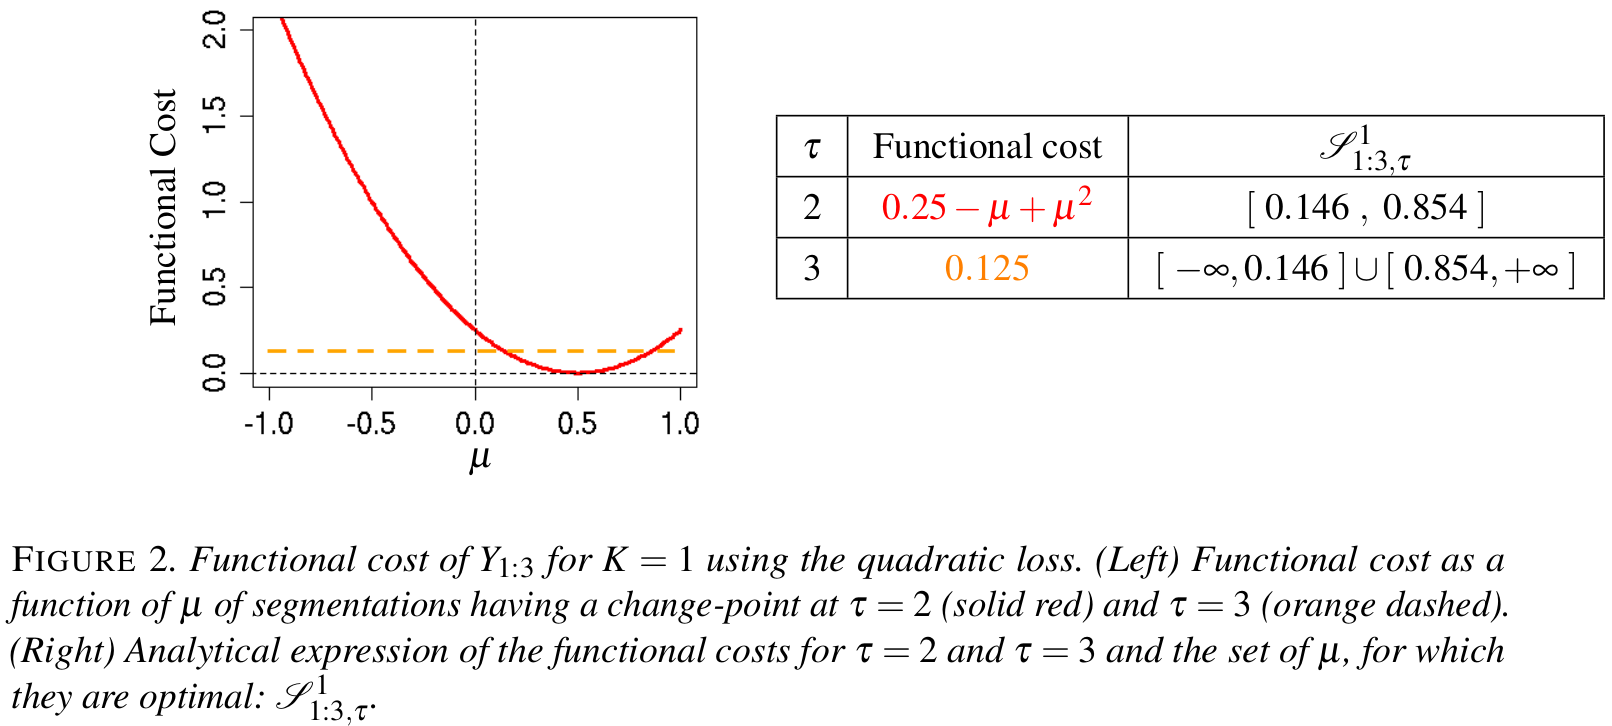
\includegraphics[width=\textwidth]{screenshot-figure-2}
\end{frame}

\begin{frame}
  \frametitle{Functional cost computation at $t=4$}
  Rigaill, arXiv:1004.0887.

  \begin{itemize}
  \item Data: 0, 0.5, 0.4, -0.5. 
  \item Computing $C_{2,4}(\mu) = \ell(\mu, z_4) + \min\{C_{2,3}(\mu),\, \mathcal
    L_{1,3}\}$:
  \item Change before $\tau=2$: $\mathcal L_{1,1} + (\mu-0.5)^2+(\mu-0.4)^2$.
  \item Change before $\tau=3$: $\mathcal L_{1,2}+(\mu-0.4)^2$.
  \item Change before $\tau=4$: $\mathcal L_{1,3}=\min_\mu (\mu-0)^2+(\mu-0.5)^2+(\mu-0.4)^2$.
  \end{itemize}

  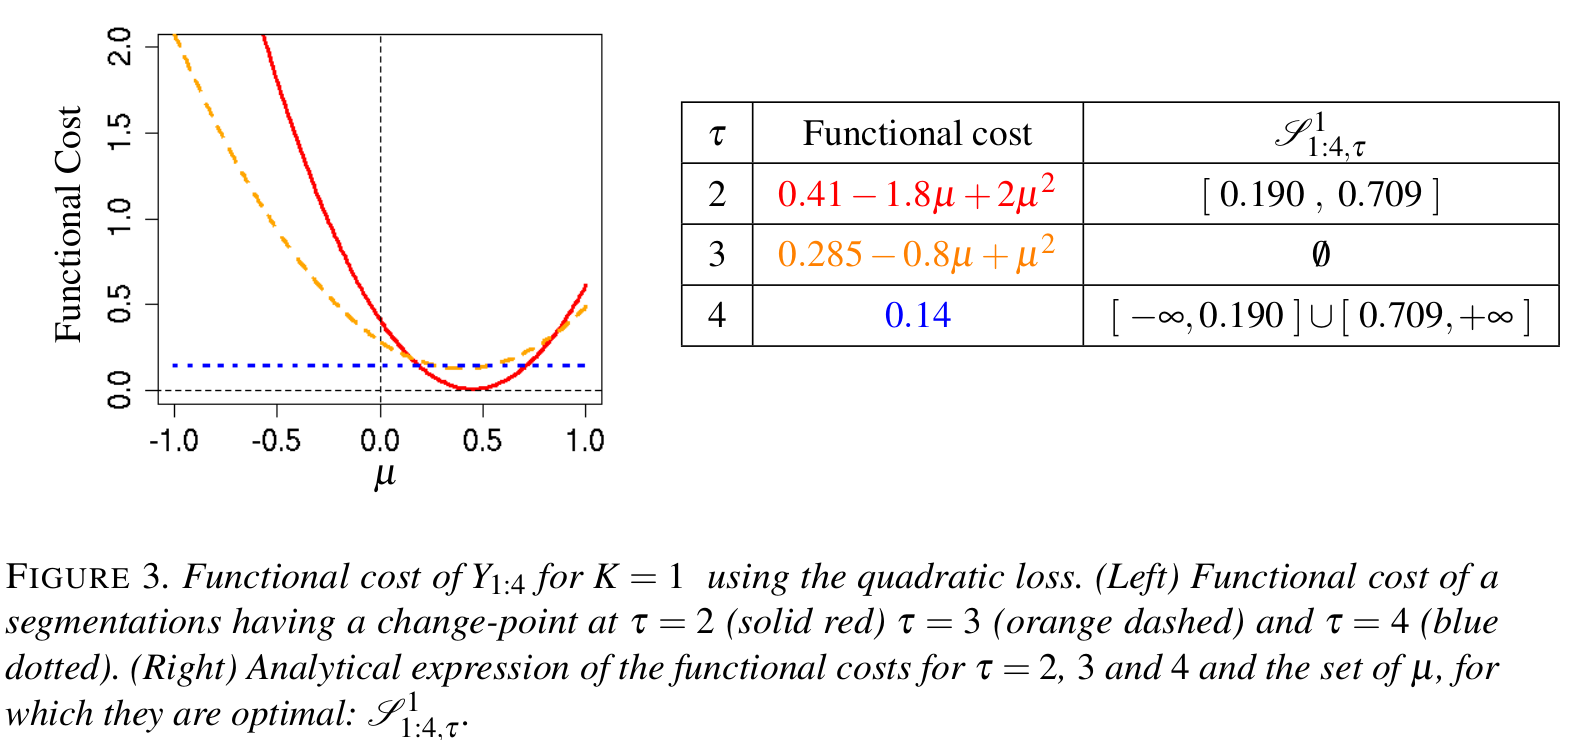
\includegraphics[width=\textwidth]{screenshot-figure-3}
\end{frame}

\begin{frame}
  \frametitle{Functional pruning larger example}

  \begin{itemize}
  \item Computing each $C_{s,t}(\mu)$ is an $O(I)$ operation where $I$
    is the number of intervals (candidate changepoints).
  \item Need to compute $O(Sn)$ functions; total complexity is $O(SnI)$.
  \item Empirically $I=O(\log n)$ due to pruning so overall $O(Sn\log n)$.
  \end{itemize}

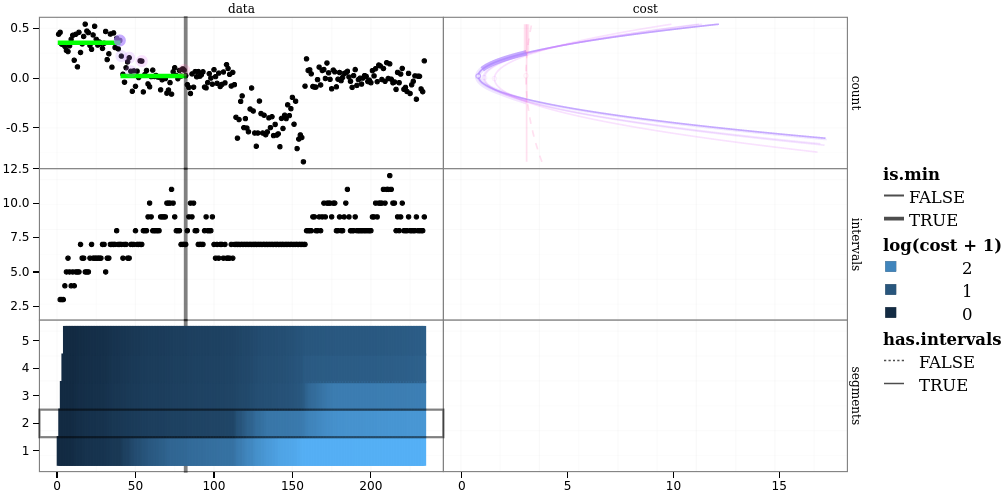
\includegraphics[width=\textwidth]{screenshot-PDPA-demo}
%    \input{figure-2-min-envelope}

\url{http://members.cbio.mines-paristech.fr/~thocking/figure-unconstrained-PDPA-normal-big/}
\end{frame}


\end{document}
